
%BEGIN_FOLD  Preamble
%oli8: this line allows me to use plain BibTex without reconfiguring my own settings.
% !TeX TXS-program:bibliography = txs:///bibtex
\documentclass{article}

%
\usepackage[preprint]{neurips_2020}
% \usepackage{neurips_2020}

\usepackage[utf8]{inputenc} % allow utf-8 input
\usepackage[T1]{fontenc}    % use 8-bit T1 fonts

\usepackage{url}            % simple URL typesetting
\usepackage{booktabs}       % professional-quality tables
\usepackage{amsfonts}       % blackboard math symbols
\usepackage{nicefrac}       % compact symbols for 1/2, etc.
\usepackage{microtype}      % microtypography
\usepackage{mathtools}		%also loads amsmath
\usepackage{amssymb, bbm}

\usepackage[format=plain,
            labelfont={sl},
            textfont={it,small}]{caption}

\usepackage{relsize}
\usepackage{environ} % http://ctan.org/pkg/environ; for capturing body as a parameter for idxmats
\usepackage{tikz}

%BEGIN_FOLD Tikz Stylings.
	\usetikzlibrary{positioning,fit,calc, decorations, arrows, shapes, shapes.geometric}
	\usetikzlibrary{backgrounds}
	\usetikzlibrary{cd}
	
	\pgfdeclaredecoration{arrows}{draw}{
		\state{draw}[width=\pgfdecoratedinputsegmentlength]{%
			\path [every arrow subpath/.try] \pgfextra{%
				\pgfpathmoveto{\pgfpointdecoratedinputsegmentfirst}%
				\pgfpathlineto{\pgfpointdecoratedinputsegmentlast}%
			};
	}}
	%%%%%%%%%%%%
	\tikzset{AmpRep/.style={ampersand replacement=\&}}
	\tikzset{center base/.style={baseline={([yshift=-.8ex]current bounding box.center)}}}
	\tikzset{is bn/.style={background rectangle/.style={fill=blue!35,opacity=0.3, rounded corners=5},show background rectangle}}

	% Node Stylings
	\tikzset{dpadded/.style={rounded corners=2, inner sep=0.7em, draw, outer sep=0.3em, fill={black!50}, fill opacity=0.08, text opacity=1}}
	\tikzset{dpad0/.style={outer sep=0.05em, inner sep=0.3em, draw=gray!75, rounded corners=4, fill=black!08, fill opacity=1}}
	\tikzset{dpad/.style args={#1}{every matrix/.append style={nodes={dpadded, #1}}}}
	\tikzset{light pad/.style={outer sep=0.2em, inner sep=0.5em, draw=gray!50}}
		
	\tikzset{arr/.style={draw, ->, thick, shorten <=3pt, shorten >=3pt}}
	\tikzset{arr0/.style={draw, ->, thick, shorten <=0pt, shorten >=0pt}}
	\tikzset{arr1/.style={draw, ->, thick, shorten <=1pt, shorten >=1pt}}
	\tikzset{arr2/.style={draw, ->, thick, shorten <=2pt, shorten >=2pt}}
	\tikzset{archain/.style args={#1}{arr, every arrow subpath/.style={draw,arr, #1}, decoration=arrows, decorate}}


	\tikzset{fgnode/.style={dpadded,inner sep=0.6em, circle},
	factor/.style={light pad}}	
	
	
	\newcommand\cmergearr[4]{
		\draw[arr,-] (#1) -- (#4) -- (#2);
		\draw[arr, shorten <=0] (#4) -- (#3);
	}
	\newcommand\mergearr[3]{
		\coordinate (center-#1#2#3) at (barycentric cs:#1=1,#2=1,#3=1.2);
		\cmergearr{#1}{#2}{#3}{center-#1#2#3}
	}
	\newcommand\cunmergearr[4]{
		\draw[arr,-, , shorten >=0] (#1) -- (#4);
		\draw[arr, shorten <=0] (#4) -- (#2);
		\draw[arr, shorten <=0] (#4) -- (#3);
	}
	\newcommand\unmergearr[3]{
		\coordinate (center-#1#2#3) at (barycentric cs:#1=1.2,#2=1,#3=1);
		\cunmergearr{#1}{#2}{#3}{center-#1#2#3}
	}

	
	\usetikzlibrary{matrix}
	\tikzset{toprule/.style={%
	        execute at end cell={%
	            \draw [line cap=rect,#1] 
	            (\tikzmatrixname-\the\pgfmatrixcurrentrow-\the\pgfmatrixcurrentcolumn.north west) -- (\tikzmatrixname-\the\pgfmatrixcurrentrow-\the\pgfmatrixcurrentcolumn.north east);%
	        }
	    },
	    bottomrule/.style={%
	        execute at end cell={%
	            \draw [line cap=rect,#1] (\tikzmatrixname-\the\pgfmatrixcurrentrow-\the\pgfmatrixcurrentcolumn.south west) -- (\tikzmatrixname-\the\pgfmatrixcurrentrow-\the\pgfmatrixcurrentcolumn.south east);%
	        }
	    },
	    leftrule/.style={%
	        execute at end cell={%
	            \draw [line cap=rect,#1] (\tikzmatrixname-\the\pgfmatrixcurrentrow-\the\pgfmatrixcurrentcolumn.north west) -- (\tikzmatrixname-\the\pgfmatrixcurrentrow-\the\pgfmatrixcurrentcolumn.south west);%
	        }
	    },
	    rightrule/.style={%
	        execute at end cell={%
	            \draw [line cap=rect,#1] (\tikzmatrixname-\the\pgfmatrixcurrentrow-\the\pgfmatrixcurrentcolumn.north east) -- (\tikzmatrixname-\the\pgfmatrixcurrentrow-\the\pgfmatrixcurrentcolumn.south east);%
	        }
	    },
	    table with head/.style={
		    matrix of nodes,
		    row sep=-\pgflinewidth,
		    column sep=-\pgflinewidth,
		    nodes={rectangle,minimum width=2.5em, outer sep=0pt},
		    row 1/.style={toprule=thick, bottomrule},
  	    }
	}
%END_FOLD

\usepackage{color}
\usepackage{hyperref}

%\usepackage{stmaryrd}

\usepackage{amsthm}
\usepackage{thmtools}

\theoremstyle{plain}
\newtheorem{theorem}{Theorem}[section]
\newtheorem{coro}{Corollary}[theorem]
\newtheorem{prop}[theorem]{Proposition}
\newtheorem{lemma}[theorem]{Lemma}
\newtheorem{fact}[theorem]{Fact}
\newtheorem{conj}[theorem]{Conjecture}

\theoremstyle{definition}
%joe11
%\declaretheorem[name=Definition,numberwithin=section,qed=$\diamond$]{defn}
%\declaretheorem[name=Construction,qed=$\diamond$,sibling=defn]{constr}
%\declaretheorem[qed=$\triangle$]{example}
\declaretheorem[name=Definition,numberwithin=section,qed=$\square$]{defn}
\declaretheorem[name=Construction,qed=$\square$,sibling=defn]{constr}
\declaretheorem[qed=$\square$]{example}

\theoremstyle{remark}
\newtheorem*{remark}{Remark}

\usepackage{xstring}
\usepackage{enumitem}

\DeclarePairedDelimiterX{\infdivx}[2]{(}{)}{%
	#1\;\delimsize\|\;#2%
}
\newcommand{\thickD}{I\mkern-8muD}
\newcommand{\kldiv}{\thickD\infdivx}

\makeatletter% Fix missing symbols i stix is loaded
\@ifpackageloaded{stix}{%
}{%
	\DeclareFontEncoding{LS2}{}{\noaccents@}
	\DeclareFontSubstitution{LS2}{stix}{m}{n}
	\DeclareSymbolFont{stix@largesymbols}{LS2}{stixex}{m}{n}
	\SetSymbolFont{stix@largesymbols}{bold}{LS2}{stixex}{b}{n}
	\DeclareMathDelimiter{\lBrace}{\mathopen} {stix@largesymbols}{"E8}%
	{stix@largesymbols}{"0E}
	\DeclareMathDelimiter{\rBrace}{\mathclose}{stix@largesymbols}{"E9}%
	{stix@largesymbols}{"0F}
}
\makeatother

%\DeclarePairedDelimiter{\ccbr}{\lBrace}{\rBrace}
%\DeclarePairedDelimiter{\bbr}{\llbracket}{\rrbracket}
%\DeclarePairedDelimiter{\ppr}{\llparenthesis}{\rrparenthesis}

\DeclarePairedDelimiterX{\bbr}[1]{[}{]}{\mspace{-3.5mu}\delimsize[#1\delimsize]\mspace{-3.5mu}}
\DeclarePairedDelimiter{\norm}{\lVert}{\rVert}

\let\Horig\H
\let\H\relax
\DeclareMathOperator{\H}{\mathrm{H}} % Entropy
\DeclareMathOperator{\I}{\mathrm{I}} % Information
\DeclareMathOperator*{\E}{\mathbb{E}} % Expectation
\DeclareMathOperator*{\argmin}{arg\;min}
\newcommand{\CI}{\mathrel{\perp\mspace{-10mu}\perp}} % Conditional Independence

\newcommand{\todo}[1]{{\color{red}\ \!\Large\smash{\textbf{[}}{\normalsize\textsc{todo:} #1}\ \!\smash{\textbf{]}}}}
\newcommand{\note}[1]{{\color{blue}\ \!\Large\smash{\textbf{[}}{\normalsize\textsc{note:} #1}\ \!\smash{\textbf{]}}}}

\newcommand\mat[1]{\mathbf{#1}}
%\newcommand{\indi}[1]{\mathbbm{1}_{\left[\vphantom{\big[}#1 \vphantom{\big]}\right]}}

% \newcommand\recall[1]{\expandarg\cref{#1}:\vspace{-1em} \begingroup\small\color{gray!80!black}\begin{quotation} \expandafter\csname #1\endcsname* \end{quotation}\endgroup }


\usepackage{environ}
\usepackage{xstring}

% Wow this works I'm brilliant
\def\wrapwith#1[#2;#3]{
	\expandarg\IfSubStr{#1}{,}{
		\expandafter#2{\expandarg\StrBefore{#1}{,}}
		\expandarg\StrBehind{#1}{,}[\tmp]
		\xdef\tmp{\expandafter\unexpanded\expandafter{\tmp}}
		#3
		\wrapwith{\tmp}[#2;{#3}]
	}{ \expandafter#2{#1} }
}
\def\hwrapcells#1[#2]{\wrapwith#1[#2;&]}
\def\vwrapcells#1[#2]{\wrapwith#1[#2;\\]}
\NewEnviron{mymathenv}{$\BODY$}

\newcommand{\smalltext}[1]{\text{\footnotesize#1}}
\newsavebox{\idxmatsavebox}
\def\makeinvisibleidxstyle#1#2{\phantom{\hbox{#1#2}}}
\newenvironment{idxmatphant}[4][\color{gray}\smalltext]{%
	\def\idxstyle{#1}
	\def\colitems{#3}
	\def\rowitems{#2}
	\def\phantitems{#4}
	\begin{lrbox}{\idxmatsavebox}$%$\begin{mymathenv}
	\begin{matrix}  \begin{matrix} \hwrapcells{\colitems}[\idxstyle]  \end{matrix}
		% &\vphantom{\idxstyle\colitems}
		\\[-0.05em]
		\left[
		\begin{matrix}
			\hwrapcells{\phantitems}[\expandafter\makeinvisibleidxstyle\idxstyle]  \\[-1.2em]
	}{
		\end{matrix}\right]		&\hspace{-0.8em}\begin{matrix*}[l] \vwrapcells{\rowitems}[\idxstyle] \end{matrix*}\hspace{0.1em}%
	\end{matrix}%
	$%\end{mymathenv}
	\end{lrbox}%
	\raisebox{0.75em}{\usebox\idxmatsavebox}
%	\vspace{-0.5em}
}

\newenvironment{idxmat}[3][\color{gray}\smalltext]
	{\begingroup\idxmatphant[#1]{#2}{#3}{#3}}
	{\endidxmatphant\endgroup}

\newenvironment{sqidxmat}[2][\color{gray}\smalltext]
	{\begingroup\idxmat[#1]{#2}{#2}}
	{\endidxmat\endgroup}


%%%%%%%%%%%%
% better alignment for cases
\makeatletter
\renewenvironment{cases}[1][l]{\matrix@check\cases\env@cases{#1}}{\endarray\right.}
\def\env@cases#1{%
	\let\@ifnextchar\new@ifnextchar
	\left\lbrace\def\arraystretch{1.2}%
	\array{@{}#1@{\quad}l@{}}}
\makeatother

\newcommand\numberthis{\addtocounter{equation}{1}\tag{\theequation}}
% end of model-commands.tex

\usepackage[noabbrev,nameinlink]{cleveref}
\crefname{example}{example}{examples}
\crefname{defn}{definition}{definitions}
\crefname{prop}{proposition}{propositions}
\crefname{constr}{construction}{constructions}
\crefname{fact}{fact}{facts}

\definecolor{deepgreen}{rgb}{0,0.5,0}
\hypersetup{colorlinks=true, linkcolor=blue!50!black, urlcolor=magenta, citecolor=deepgreen}

\usepackage{float}
\usepackage{subcaption}
	\captionsetup[subfigure]{subrefformat=simple,labelformat=simple}
	\renewcommand\thesubfigure{(\alph{subfigure})}
	
\usepackage{comment}
% Wrap definitions...
\definecolor{fulldefncolor}{rgb}{0.7,0.7,.7}
\specialcomment{fulldefn}{\begingroup\color{fulldefncolor}\begin{defn}}{\end{defn}\endgroup}
\definecolor{quickdefncolor}{rgb}{0.7,0.7,.7}
\specialcomment{quickdefn}{\begingroup\color{quickdefncolor}\begin{defn}}{\end{defn}\endgroup}

%END_FOLD

%%%% Version knobs %%%%%. 

\excludecomment{notfocus}

\definecolor{vfullcolor}{gray}{0.7}
\specialcomment{vfull}{\begingroup\color{vfullcolor}}{\endgroup}
\excludecomment{vfull} %\includecomment{vfull}

\excludecomment{vleftovers}
% \definecolor{vleftoverscolor}{gray}{0.85}
% \specialcomment{vleftovers}{\begingroup\color{vleftoverscolor}}{\endgroup}

\excludecomment{vcat} %\includecomment{vcat}
\excludecomment{vnotation} %\includecomment{vnotation}

%BEGIN_FOLD
\definecolor{notationcolor}{rgb}{0.9,0.9,.9} % purple
\newcommand{\notation}[2][]{#1}
\begin{vnotation}
	\renewcommand{\notation}[2][]{{\color{notationcolor} #2}}
\end{vnotation}

\newcommand{\commentout}[1]{\ignorespaces}
\newcommand{\vfullfootnote}[1]{}
\begin{vfull}
\renewcommand{\vfullfootnote}[1]{\footnote{#1}}
\end{vfull}


%oli8: disable tikz externalization for now, dependence on etoolbox
% \usepackage{etoolbox}
% \usetikzlibrary{external}
% \tikzexternalize[prefix=tikz/]  % activate!
% %
% \AtBeginEnvironment{tikzcd}{\tikzexternaldisable} %... except careful of tikzcd...
% \AtEndEnvironment{tikzcd}{\tikzexternalenable}

%\crefname{section}{\S\!}{\S\!}
%\addbibresource{../refs.bib}
%\addbibresource{../uncertainty.bib}
%\addbibresource{../maths.bib}
%\addbibresource{graphical-models.bib}

%%%%%%%%%%%%%%%% SHORTCUTS FOR COMMONLY USED THINGS %%%%%%%%%%%%%%


% Semantics
% use sd for... Set of Distributions / Score of Distributions / Single Distribution?
%\DeclarePairedDelimiter{\SD}{\llbracket}{\rrbracket_{\text{sd}}}
\DeclarePairedDelimiterXPP{\SD}[1]{}{[}{]}{_{\text{sd}}}{\mspace{-3.5mu}\delimsize[#1\delimsize]\mspace{-3.5mu}}
		
\newcommand{\none}{\varobslash}
\def\sheq{\!=\!}
\DeclareMathOperator\dcap{\mathop{\dot\cap}}
\newcommand{\tto}{\rightarrow\mathrel{\mspace{-15mu}}\rightarrow}

\newcommand{\bp}[1][L]{\mat{p}_{\!_{#1}\!}}
\newcommand{\V}{\mathcal V}
\newcommand{\N}{\mathcal N}
\newcommand{\Ed}{\mathcal E}
\newcommand{\pdgvars}[1][]{(\N#1, \Ed#1, \V#1, \mat p#1, \beta#1)}

% What about script?
% \newcommand{\dg}[1]{\mathit{#1}}
% \usepackage[mathscr]{euscript}
% \newcommand{\dg}[1]{\mathscr{#1}}
%or dutchcal?
\DeclareMathAlphabet{\mathdcal}{U}{dutchcal}{m}{n}
\DeclareMathAlphabet{\mathbdcal}{U}{dutchcal}{b}{n}
%joe10: I can live with this, but this was NOT a good use of your
%time.  It wouldn't be a problem if your time choices affected only
%you -- it's your life, you can spend your time as you see fit. But
%they are affecting me, and forcing us to do things in the last
%minute.  This is bad.
%joe1:out of curiousity, why not use \mathcal?  That's what you use
%for BNs.  Why do PDG use a different font?
\newcommand{\dg}[1]{\mathbdcal{#1}}
\newcommand{\var}[1]{\mathsf{#1}}
\newcommand\Pa{\mathbf{Pa}}

% \newcommand\IBal{\mathit{IF}}
%oli11: I'm now realizing I unintentionally reverted the naming choice
%(I was looking for something new and changed my name a lot). I don't
%care all that much what you change it to but ideally it would retain
%the G- in front (the subscripts / superscripts don't look as good,
%and we're trying to emphasize fixed model), not start with I (because
%Inc does), and have some lower case letters, for stylistic
%coherence. 
%joe10: I think that ``balance'' sends the wrong message, and t's more
%standard to have the G as a subscript.  To my eyes, it looks ugly in
%the front.  
%\newcommand\IBal[1][{\dg M}]{#1\text-\mathit{IBal}}
%joe11: given your name change
%\newcommand{\IBal}[1]{\mathit{IDiff}_{#1}}
%oli15: global command change "\IBal => \IDef"
\newcommand{\IDef}[1]{\mathit{IDef}_{#1}}

\newcommand\extrainfo[2][\dg M]{\IDef[#1](#2)}
% \newcommand\Inc[2][\dg M]{\Incsymb(#2;#1)}
%oli10: changed name of command everywhere.
\newcommand\Inc{\mathit{Inc}}


%oli8: The injection of BNs as PDGs. I wanted something more mnemonic,
% but discovered it made formulas much longer and uglier.
%\newcommand\PDGof{\mathit{PDG}}
%joe7*: Since we use \M to denote a PDG, this should be M_B, not
%\Gamma(B).  Can you change it everywhere?
%joe8*: I changed it
%oli10: I've gone through and fixed the sites that didn't get converted properly.
%\newcommand\PDGof{\Gamma}
%oli10: The notation M_B to me suggests to me that somehow B is
%indexing the data in M. 
%  I like notation that to keep separate a particular pdg M, M', maybe
%  N, L also (fraktur font) and a the function that converts them. To
%  also satisfy your desire that it be visually clear that the result
%  is a PDG, I propose naming the function in fraktur font.
%joe9*: NO!!  Oliver, you're entitled to your esthetic, but in this
%ccase I will impose my esthetic tastes on you, because I'm quite
%convinced that you are an extreme outlier.  In general, good notation
%will mke it clar what kind of an object someting is.  If we're using
%{\dg M} to denote PDGs, we should continue to do so when dentoting
%the PDG that represents a BN.  Second, Fraktur is forbidding.
%There's a good reason you see it so rarely.  Ask your friends.
%
%oli11-notation: Notation rant to follow. 
% If you have a collection of BNs, I would agree that naming the
% associated PDG \dg M_{B} is the right thing to do, because it
% emphasizes the dependence, and is defined in a scope where it won't
% contaminate the meaning of "$\dg M$"" in general.  
% Your notation takes this to an extreme I find unpalatable. You use
% this subscript notation for the general function which returns (by
% analogy) the PDG associated to an arbitrary, as of yet undefined
% PDG, which could be stored in any symbol. Therefore, M_{<symbol>} is
% bound to the conversion function, but M_1, M_2 are also used, and so
% is just normal M. I find this difficult to read. I also know for a
% fact that more than one student in your RaU class has been confused
% that the function that transforms things is the conflated with its
% output and other unrelated variables, and that a mere notational
% change improved things. It is just a mathematical fact that by
% naming things this way, the grammar you define ceases to be
% context-free, which makes it harder to parse. It also is now almost
% impossible to refer to the mathematical object corresponding to the
% funtion (e.g., which takes a factor graph and returns a PDG: the
% standard use of placeholders would give [ - ]_[.], which is
% certainly useless). The subscript also prevents you from then having
% indexed collections of models in general, because M_i now means
% transform i (and the indexed set could be indexed by a collection of
% bayesian networks...), and doesn't typecheck. IF you use M(X)
% instead, you have similar issues, and the paranetheses keep you from
% being able to use a model as a function (I woulld like to be able
% to write {\dg M) (Y \mid X)).  
%
% Two more, even scarier effects. First: what do you do if you have
% {\dg M} in scope, and want to convert a factor graph? Shouldn't {\dg
% M}(\Phi) or {\dg M}_{\Phi} have some dependence on {\dg M}? It sure
% looks like it does.  
% Second: you also have to be MUCH more careful to verify coherence
% properties. Every time you define $M_X$ for a new class of objects
% $X$, you have to be very careful that every detail of the conversion
% exactly lines up; you otherwise have to write . Now \Gamma, \Gamma'
% might not be super readable and I am sympathetic to that complaint,
% but it is always clear what computation is occuring, and which
% function is being used. If you are good about structuring your
% document and defining things, \Gamma will quickly become a part of
% the reader's langauge just as quickly (I argue more quickly if you
% use it often, because there are fewer symbols and no subtleties) as
% M_B. 
%
%I find this particular bit of notation, which I acknowledge that you
%have been using consistently, to be very poor for more reason than
%just aesthetics, and on principle I would like to avoid adopting it
%if I can. 
% I admit that fraktur font is intense, but I think that using a wide
% variety of visual symbols makes it WAY easier to track. 
% Finally, you might be surprised to learn that when I show people my
% work, I often get a surprising number of complements /specificlaly/
% regarding my notation. I can think of instances of this happening
% spontaneously, coming from category theorists, physicists, ML
% people, and even one of your students. Regularly my friends go so
% far as to accuse graders of giving me higher scores just because my
% assignment is prettier. I know I sometimes make dumb decisions, and
% my notation can become inconsistent especially when I write
% something over a long period of time (though I always plan on making
% it uniform eventually), but I believe that I'm actually way better
% than average at coming up with notation that (at least certain
% people) really like.  
% Bottom line: We seem to be on the opposite ends of some notation
% spectrum, but I also care a lot about notation. I am bad at many
% things, including focusing, and telling stories in straight lines,
% but I want you to know that in general, choosing notation is not one
% of my weaknesses. 
%joe10: maybe so, but I still find fraktur forbidding, and I suspect
%I'm not alone, and I absolutely insist that anything that is a PDG
%shoudl have an M, to remind readers that it is a PDG.  If it's
%related to a BN B, it also needs a B.  And you had many better things
%to do with your time than to write this rant ...  Reverting back to
%my preference, and asserting executive privilege.  PLEASE DO NOT
%SPEND MORE TIME ON THIS!  When you write papers without me, you can
%do as you please.
\newcommand{\PDGof}[1]{{\dg M}_{#1}}
%\newcommand{\PDGof}[1]{\dg G(#1)}
%oli10: My second choice is keeping everything with M and using parentheses, which is what I did with factor graphs. I would have preferred to do it like I suggest above with factor graphs too, but there are only so many fonts and it's not a paper on factor graphs.... This option is commented below:
%joe9: This is acceptable
%oli11: Because this is the function and not its output, and  {\dg
%M}. is already used for PDGs, I want this to be called something {dg
%M}. Some more suggestions.  
%oli11: Option 1. use mathit "pdg" (with kearning adjustment so it's
%more compact and the g does not appear offset) 
% \newcommand{\PDGof}[1]{{\mathit{p\kern-0.145em d\kern-0.17em g}} (#1)}
%oli11: option 2: same font as {\dg M}
%joe10*: NO!  while this is better, but I still have a preference for
%using notation that makes it look like a PDG.  And I find it annoying
%to be spending time on this now
%\newcommand{\PDGof}[1]{{\mathdcal{p\kern-0.05em d\kern-0.125em g}} (#1)}
%oli11: option 3: bold version
% \newcommand{\PDGof}[1]{{\mathbdcal{p\kern-0.05em d\kern-0.125em g}} (#1)}

%oli11: better kearning and spacing
% \newcommand{\ed}[3]{#2 \xrightarrow{\!\!\smash{#1}} #3}
%joe10: why are you wasting time on this when you have so many more
%important things that need to be done for this paper
\newcommand{\ed}[3]{#2
  \overset{\smash{\mskip-5mu\raisebox{-1pt}{$\scriptscriptstyle
        #1$}}}{\rightarrow} #3} 
%oli11: so now we can use this version...
\newcommand{\alle}[1][L]{_{ \ed {#1}XY}}
% \newcommand{\alle}[1][L]{_{ X \xrightarrow{\!\!#1} Y }}

%%%%%%%%%%%%%%%%%%%%%%%%%%%%%%%%%%%%%%%%%%%%%%%%%%%%%%%%%%%%%%%%%%


%%% What do I even call them anyway?
\newcommand{\ModelName}{Probabilistic Dependency Graph}
\newcommand{\modelname}{probabilistic dependency graph}
\newcommand{\modelnamehyper}{probabilistic dependency hypergraph}
\newcommand{\modelnames}{\modelname s}

%oli11**: Please do not kill my align environments. Uncomment these lines instead
% \renewenvironment{align*}{\begin{equation*}\begin{array}{rlr}}{\end{array}\end{equation*}}
%joe10: For what it's worth, I do not like your intertext.  I think it
%often makes things worse.
%oli12: Do you mean the way I use it, the way it looks in my pdf, or
%difficulty in editing / compiling?
%joe11: the first two
% \renewcommand\intertext[1]{\\\text{#1}\\}

	\newenvironment{oldthm}[1]{\par\noindent{\bf Theorem #1.} \em \noindent}{\par}
	\newenvironment{oldlem}[1]{\par\noindent{\bf Lemma #1.} \em \noindent}{\par}
	\newenvironment{oldcor}[1]{\par\noindent{\bf Corollary #1.} \em \noindent}{\par}
	\newenvironment{oldpro}[1]{\par\noindent{\bf Proposition #1.} \em \noindent}{\par}
	\newcommand{\othm}[1]{\begin{oldthm}{\ref{#1}}}
	\newcommand{\eothm}{\end{oldthm} \medskip}
	\newcommand{\olem}[1]{\begin{oldlem}{\ref{#1}}}
	\newcommand{\eolem}{\end{oldlem} \medskip}
	\newcommand{\ocor}[1]{\begin{oldcor}{\ref{#1}}}
	\newcommand{\eocor}{\end{oldcor} \medskip}
	\newcommand{\opro}[1]{\begin{oldpro}{\ref{#1}}}
	\newcommand{\eopro}{\end{oldpro} \medskip}
%oli11: can all be replaced by ...
%joe10: fine.  So you spent a lot of time to simplify a macro.  THIS
%WASN'T WORTH IT!
%oli12: this particular detour took me all of 45 seconds. 
%joe11: But you surely spent time thinking about it ...
	\newenvironment{old}[1]{\par\noindent{\bf \Cref{#1}.} \em \noindent}{\par\medskip}
%oli15
%fixing up restatables so links happen automatically via the above.
\usepackage{xpatch}
\makeatletter
\xpatchcmd{\thmt@restatable}% Edit \thmt@restatable
    {\csname #2\@xa\endcsname\ifx\@nx#1\@nx\else[{#1}]\fi}% Replace this code
    % {\ifthmt@thisistheone\csname #2\@xa\endcsname\typeout{oiii[#1;#2\@xa;#3;\csname thmt@stored@#3\endcsname]}\ifx\@nx#1\@nx\else[#1]\fi\else\csname #2\@xa\endcsname\fi}% with this code
    {\ifthmt@thisistheone\csname #2\@xa\endcsname\ifx\@nx#1\@nx\else[{#1}]\fi
    \else\fi}
    {\typeout{oii Success1?}}{\typeout{oiii failure1?}} % execute code for success/failure instances
\xpatchcmd{\thmt@restatable}% Edit \thmt@restatable
    {\csname end#2\endcsname}
    {\ifthmt@thisistheone\csname end#2\endcsname\else\fi}
    {\typeout{oii Success2?}}{\typeout{oiii failure2?}}
\newcommand{\recall}[1]{\smallskip\par\noindent{\bf \expandarg\Cref{thmt@@#1}.} \begingroup\em \noindent
%joe14
% \expandafter\csname#1\endcsname* \endgroup\par\medskip}
   \expandafter\csname#1\endcsname* \endgroup\par\smallskip}
\makeatother
%oli16: The extra space was because there was extra space in the paragraph, not
%because this length was too big. By breaking arrays, everything will be better.
\allowdisplaybreaks

% \newcommand{\begprop}[1]{\begin{prop}[restate=#1,label=#1]}
\newcommand{\begthm}[2]{\begin{#1}[restate=#2,label=#2]}
%oli15 end thmtools magic.



\numberwithin{equation}{section}

\title{Probabilistic Dependency Graphs}
\author{} % LEAVE BLANK FOR ORIGINAL SUBMISSION.

%% UAI  reviewing is double-blind.
%
%% The author names and affiliations should appear only in the accepted paper.
%%
%\author{
%	{\bf Oliver E. Richardson%\thanks{Footnote for author to give an alternate address.}
%		}\\
%%	Computer Science Dept. \\
%	Cornell University\\
%	Address\\
%\And
%	{\bf Joseph Y. Halpern}  \\
%	Cornell University      \\
%	Address \\
%}
%

%END_FOLD
\begin{document}
\maketitle
\begin{abstract}
We introduce Probabilistic Dependency Graphs (PDGs), a new class of
directed graphical models.   PDGs can capture inconsistent beliefs in a
natural way and are more modular than Bayesian Networks (BNs), in that
they make it easier to incorporate new information and restructure the  
representation.    We show by example how PDGs are an especially natural
modeling tool.
%
We provide three semantics for PDGs, each of which can be derived from a
scoring function (on joint distributions over the
variables in the network) that can be viewed as representing a
distribution's incompatibility with the PDG. For the PDG corresponding
to a BN, this function is  uniquely minimized by the distribution the BN
represents, showing that PDG semantics extend BN semantics.
A slight variant of the scoring function (which does not affect the
score of a distribution that represents a BN) yields the variational
free energy of general factor graphs; we use this to explain how PDGs
and factor graphs generalize BNs in orthogonal directions.%
\end{abstract}

\section{Introduction}

In this paper we introduce yet another graphical for modeling beliefs,
\emph{Probabilistic Dependency Graphs} (PDGs). There are already many
such models in the literature, including Bayesian networks (BNs) and
factor graphs. (For an overview, see \cite{KF09}.)
Why does the world need one more?  

Our original motivation for introducing PDGs was to be able capture
inconsistency. We want to be able to model the process of resolving
inconsistency; to do so, we have to model the inconsistency itself. But our
approach to modeling inconsistency has many other advantages. In particular,
PDGs are significantly more modular than other directed graphical models:
operations like restriction and union that are easily done with PDGs are
difficult or impossible to do with other representations.

We start with some examples to motivate PDGs and illustrate some of these properties.  

\begin{example} \label{ex:guns-and-floomps}
%oli12: Introduce our protagonist earlier. Changes to pronouns have
%been made throughout example. 
% You arrive in a foreign country known for having very clear laws. From
% prior reading, you ascribe probability 0.95 to owning guns being
% against the law. Upon arrival, you end up talking to some teenagers
% who use the local slang, after which you believe that with probility
% .1, the law prohibits floomps.  
Grok is visiting a neighboring district. From prior reading, she thinks it likely (probability
.95) that guns are illegal here. Some brief conversations with locals lead her to believe believe with
probility .1, that the law prohibits floomps.

% The obvious way to represent this as a BN involves two binary random variables,
% $F$ (taking values $\{f, \overline f\}$), indicating the legality of floomps,
% and $G$ (taking values $g, \overline g$) indicating the legality of guns. 
The obvious way to represent this as a BN is to use two random variables
$F$ and $G$ (respectively taking values $\{f, \smash{\overline f}\}$ and $g, \overline g$), indicating the respective legalities of owning floomps and guns.
%oli12 no paragraph break here.
The semantics of a 
%oli12
% Bayes Net
BN
offer her two choices: either assume that $F$ and $G$
% are independent and give (unconditional) probabilities of $F$ and $G$, or we
to be independent and give (unconditional) probabilities of $F$ and $G$, or
choose a direction of dependency, and give one of the two unconditional
probabilities and a conditional probability distribution. 
%oli12:
% As there is no reason
% to believe that either variable depends on the other, 
As there is no reason to choose either direction of dependence, the
natural choice is to 
assume independence, giving her the 
%oli12: combining figures
BN on the left of \Cref{fig:gun-floomp-diagram}.
%following BN

%oli12
% Now suppose that you later discover that
A traumatic experience a few hours later leaves Grok believing that
%joe11
%``floomp'' is likely (92\%) to be another word for gun.
``floomp'' is likely (probability .92) to be another word for gun.
%oli12: I've removed the directionality by adding arrows in both directions.
%, and come to believe that if floomps are legal (resp., illegal), then
% there's a  chance guns are as well, and vice versa. 
%joe7: r seems like a atrange letter to use, although it's not a big deal
%oli12: I don't care about the letter. let's use p? Also this notation, while 
% you might not like it, is the consensus, especially in the conference we're 
% submitting to. We're already giving them something quite out of the ordinary;
% I don't want  to push it too far.  It's also expedient here as it lets us 
% immediately indicate the direction.
Let $p(G \mid F)$ be the \emph conditional \emph probability \emph
distribution (cpd) that describes 
the belief that if floomps are legal (resp., illegal),
%joe11
%then with 92\% probability, guns are as well, and $p'(F \mid G)$ be
then with probability .92, guns are as well, and $p'(F \mid G)$ be
the reverse. 
%oli12:
% A first reaction might be to
Starting with $p$, Grok's first instinct is to
simply incorporate the conditional information by adding $F$ as a parent of
$G$, and then associating
the cpd
$p$ with $G$. But then what should she do
with the original probability she had for $G$?  Should she just discard it?
It is easy to check that there is no 
%oli12
% probability distribution 
joint distribution
that is consistent with
%oli12 inserted
both
the two original priors on $F$ and $G$ and also 
%oli12: already lots of commas in this sentence. saying "the cpd" too often also gets to be a lot....
%the cpd $\mat r$, so if she
%joe11
%$p$---so if she
$p$.  So if she
is to represent the information with a BN, which always represents a consistent
distribution, she must resolve the inconsistency.  

However,
%oli12: rewrote paragraph.
% it may be better not to sort this out right away. 
% How to resolve it may be clearer 
% if you can get confirmation that guns are indeed floomps, or read the
% laws more carefully.
sorting this out immediately may not be ideal.
For instance, if the inconsistency arises from a conflation between
two definitions 
of ``gun'', a resolution will have destroyed the original cpds. A
better use of computation may be to notice the inconsistency and look
up the actual law. 

By way of contrast, consider the corresponding PDG. In a PDG, the cpds are
attached to edges, rather than nodes of the graph.
%oli12: this discussion is a distraction; it has nothing to do with PDGs over BNs.
 % we don't mention matrices anywhere else anymore, and the matrix representation
 % in the figure is both a common and inutuitive way of describing this
%
% The cpd associated with an
% edge $e$ from $X$ to $Y$ is a matrix $\mat e$, where the element $\mat e_{x,y}$
% at row $x$ and column $y$ is the conditional probability $\Pr(Y \!\!=\!\!y \mid
% X \!\!=\!\! x)$. 
In order to represent unconditional probabilities, we introduce
a \emph{unit variable} $\var 1$ which 
%oli12: no reason to be too verbose here; more important stuff is coming.
% takes on only one possible value, which we denote
takes only one value, denoted
$\star$. 
%oli12: Thus, we have
This leads Grok to 
the PDG depicted in \Cref{fig:gun-floomp-diagram},
where the edges from $\var 1$ to $F$ and $G$ are associated with the
unconditional probabilities of $F$ and $G$, and the 
%oli12
%edge from $F$ to $G$ is associated with the cpd $p$. 
edges between $F$ and $G$ are associated with $p$ and $p'$.

%oli12: Combining the two figures, squeezing digarms together further.
\begin{figure}[htb]
%joe11*: why are some parts of the figure in light gray?  I would prefer
%to make it all black.  If we use a different color, we have to
%explain why.  
  \centering
	\scalebox{0.8}{
    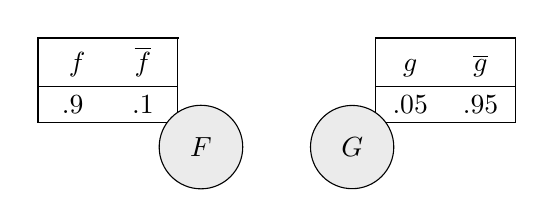
\begin{tikzpicture}[scale=0.8,ampersand replacement=\&]
        
        \matrix [table with head, column 1/.style={leftrule}, anchor=south east,
             column 2/.style={rightrule}, row 2/.style={bottomrule}] at (-1.4,0.22) {
            \vphantom{$\overline fg$} $f$ \& \vphantom{$\overline fg$}$\overline f$\\
            .9 \& .1\\
        };
        \matrix [table with head, column 1/.style={leftrule}, anchor=south west,
             column 2/.style={rightrule}, row 2/.style={bottomrule}] at (1.4,0.22) {
             \vphantom{$\overline fg$}$g$ \& \vphantom{$\overline fg$}$\overline g$\\
             .05 \& .95\\
        };
        \node[dpadded, circle, fill=black!08, fill opacity=1] (floomp) at (-1.2,0) {$F$};
        \node[dpadded, circle, fill=black!08, fill opacity=1] (gun) at (1.2,0) {$G$};
    \end{tikzpicture}
    ~~\vrule~~
	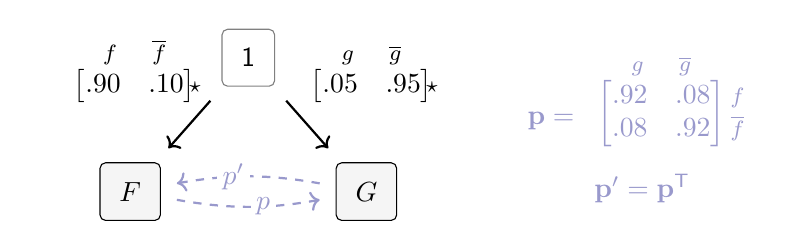
\begin{tikzpicture}
		\node[dpadded, fill=white, draw=gray] (true)  at (0,1.7) {$\var 1$};
		\node[dpadded] (floomp) at (-1.5,0) {$F$};
		\node[dpadded] (gun) at (1.5,0) {$G$};			
		
		\draw[arr] (true) -- coordinate(A) (floomp);
		\draw[arr] (true) -- coordinate(B) (gun);

		\node[above left=2.8em of A, anchor=center] {
        %oli14 fix gray.
			% \begin{idxmat}{\!\!\!$\star$\;\;\;}{$f$, $\overline f$}
			\begin{idxmat}[\color{black}\smalltext]{\!\!\!$\star$\;\;\;}{$f$, $\overline f$}
				.90 & .10 \\
			\end{idxmat}
		};
		\node[above right=2.8em of B, anchor=center] {
        %oli14
        % \begin{idxmat}{\!\!\!$\star$}{$g$, $\overline g$}
			\begin{idxmat}[\color{black}\smalltext]{\!\!\!$\star$}{$g$, $\overline g$}
				.05 & .95 \\
			\end{idxmat}
		};
		\definecolor{heldout}{rgb}{0.6, 0.6, .8}	
		\draw[heldout, dashed, arr] (floomp) to[bend right=10] node[pos=0.6, fill=white, inner sep=2pt] (C) {$p$} (gun);
        %oli12: addes reverse arrow, edited the above line with a yshift.
        \draw[heldout, dashed, arr] (gun) to[bend right=10] node[pos=0.6, fill=white, inner sep=2pt] {$p'$} (floomp);
		\node[anchor=center] (newcpd) at (5, 1.2) {
			\color{heldout}
			$\mat p =\!\!\!$\begin{idxmat}[\color{heldout}\smalltext]{$f$,$\overline f$}{$g$, $\overline g$}
%joe12
%			  .92 & 0.08 \\ .08 & .92 \\
			  .92 & .08 \\ .08 & .92 \\
			\end{idxmat}
		};
        \node[below=3pt of newcpd] {\color{heldout}$\mat p' = \mat p^{\textsf T}$};
	\end{tikzpicture}
	}
    %oli12 update caption accordingly.
    %oli12: note before editing caption: making it fit on one line is not easy.
	% \caption{An inconsistent PDG, requiring resolution}
%joe11
%        \caption{A BN (left), and respective PDG (right), which can
        \caption{A BN (left) and corresponding PDG (right), which can
        include more cpds; $p$ or $p'$ make it inconsistent.} 
    \label{fig:gun-floomp-diagram}
\end{figure}

%joe11: if we make everything black, we should get rid of ``black'' in
%the next line.
The original state of knowledge consists of all three nodes and the two
%oli13: the important bit is that they're solid. I'm trying to
%linguistically  exclude the blue/ dashed lines.
% black
solid
edges from $\var 1$. This is like Bayes Net that we considered above,
%joe11
%except we
except that we 
no longer
%oli12! 
explicitly
%joe11
%oli13:  :(  I think "to be" sounds way better. It's shorter, it doesn't expend
% our limited supply of "and", "that" and "are", which tiring quickly. It sounds
% cooloer. That's also definitely how I would say it in person; I
% think the "that 
% ... are" sounds like you're talking to someone you only trust to know simple 
% grammar --- but in fact, "to be" often taught earlier when people learn English
% as a foreign language, so this form is shorter and without an accesibility 
% cost.
% I believe the infinitive also strengthens the statement by not implying a 
% present tense (how is time relevant here?). I'm changing it back. If you have 
% a reason for your aesthetic preference that you think objectively outweighs this
% consideration to a significant degree, you can change it back and I will 
% accept it without argument, but ask you why later.
%
% assume that $F$ and $G$ are independent; we merely record the constraints
%joe12: if you must have ``to be''
%assume $F$ and $G$ to be independent; we merely record the constraints
take  $F$ and $G$ to be independent; we merely record the constraints
imposed by the given probabilities.  
	
The key point is that we can incorporate the new information into our original
representation (the graph in \Cref{fig:gun-floomp-diagram} without the edge from
$F$ to $G$) simply  by adding the edge from $F$ to $G$ and the associated cpd
%joe12: I could accept that the new information is in gray but then
%why are f and \overline{f}, g nad \overline{g}, and * in gray?
%oli14: Fixed. The reason is because I didn't want to draw focus towards the labels.
%$\mat r$. Doing so does not change the meaning of the original edges.  
%oli14:
% $\mat p$ (the new infromation is shown in gray). 
$p$ (the new infromation is shown in blue).
Doing so does not change the meaning of the original edges.   
%oli12: redundant.
% This
% presentation lets us simply include information, and resolve inconsistencies
% later.
Unlike a Bayesian update, the operation is even reversible: all we need
to do recover our original belief state is delete the new edge, 
%oli12: no need for 'effectively'
%effectively
making it possible to mull over and then reject an observation.
%
\end{example}


The ability of PDGs to model inconsistency, as illustrated in
\Cref{ex:guns-and-floomps}, appears to have come at a significant cost. We seem
to have lost a key benefit of BNs: the ease with which they can
capture
(conditional) independencies, which, as Pearl \cite{pearl1989conditional} has
argued forcefully, are omnipresent.
%oli12*: it seems like we should add a sentence fragment here, along
%the lines of "but we will be able to easily recover them".  Also, the
%above is kind of redundant, so I keep looking at it trying to figure
%out how to re-word, but it's so well written that I can't figure out
%what I want to do to it.
%joe11: how about:
%As we shall see, we will be able to recover this information.
%oli13: Most anything we add without cutting down the text before will
%ultimately cost a line. I'm not sure this particular phrase is worth
%it, I've commented it out. 
% Counterproposal:
%joe12: Looks like you didn't finish this here
%joe13*: you still didn't finish this sentence.  I'm cutting it.
%And yet:
%oli15: The intention was to lead directly to the example. It's a
%clever but maybe  
% too-cute transition; it is free (fits on on the line) if you remove a comma. 


% most of the time, we do not make the independence
% assumption in a bn because we know for certain that the
% variables are independent; rather, we just suspect that the
% identified edges are by much more important than the
% others. determining for sure that smoking  and second hand
% smoke are independent, controlling for parents' smoking
% habits, would extremely difficult, and would require
% empiricism to validate. 
	

\begin{example}[emulating a BN]\label{ex:smoking}

We now consider the classic (quantitative) Bayesian network $\cal B$, which has
four binary variables indicating whether a person ($C$) develops cancer, ($S$)
smokes, ($\mathit{SH}$) is exposed to second-hand smoke, and ($\mathit{PS}$) has
parents who smoke, presented graphically in \Cref{subfig:smoking-bn}. We now
walk through what is required to represent $\cal B$ as a PDG, which we call
$\PDGof{{\mathcal B}}$, shown as the solid nodes and edges in
\Cref{subfig:smoking-pdg}. 

\begin{figure*}[ht!]
	\centering
	
	\begin{subfigure}[b]{0.25\textwidth}
		\scalebox{0.9}{
        %oli12: update BN figure to be consistently shaped
		\begin{tikzcd}[center base, column sep=1.0em, row sep=0em, dpad={fill opacity=1,fill=black!08, circle, inner sep=3pt, minimum size=2.3em, draw=gray}, 
			ampersand replacement=\&]
		\& S \ar[dr] \\
		PS \ar[ur]\ar[dr] \&\& C \\
		\& SH \ar[ur]
		\end{tikzcd}}
        \caption{The Bayesian network $\cal B$}
		\label{subfig:smoking-bn}
	\end{subfigure}%
	\hspace{1.5em}\vline\hspace{1.5em}
	\begin{subfigure}[b]{0.57\textwidth}
		\scalebox{0.9}{
		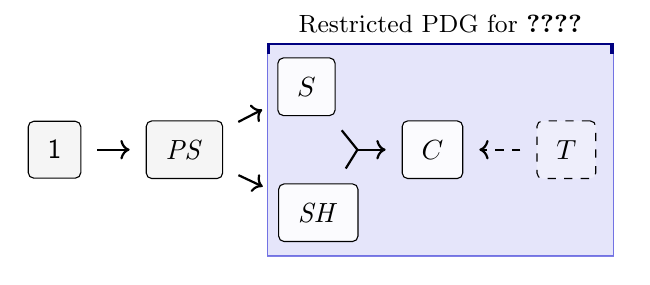
\begin{tikzpicture}[center base]
		\fill[fill opacity=0.1, blue!80!black, draw, draw opacity=0.5] (2.7,1.35) rectangle (7.1, -1.35);
		
		\node[dpadded] (1) at (0,0) {$\var 1$};
		\node[dpadded] (PS) at (1.65,0) {$\mathit{PS}$};
		\node[dpadded, fill=black!.16, fill opacity=0.9] (S) at (3.2, 0.8) {$S$};
		\node[dpadded, fill=black!.16, fill opacity=0.9] (SH) at (3.35, -0.8) {$\mathit{SH}$};
		\node[dpadded, fill=black!.16, fill opacity=0.9] (C) at (4.8,0) {$C$};
		
		\draw[arr] (1) -- (PS);
		\draw[arr] (PS) -- (S);
		\draw[arr] (PS) -- (SH);
		\mergearr{SH}{S}{C}
		
		\node[dpadded, fill=black!.16, fill opacity=0.35, dashed] (T) at (6.5,0) {$T$};
		\draw[arr,dashed] (T) -- (C);	

		\draw[very thick, |-|, color=blue!50!black,text=black] (2.7, 1.35) --coordinate(Q) (7.1,1.35);
        \fill[white] (2.6, 1.36) rectangle (7.2,1.55);
        \useasboundingbox (current bounding box);
        \node[above=0.05em of Q]{\small Restricted PDG for \Cref{ex:grok-ablate,ex:grok-union}};
		
		\end{tikzpicture}}

%oli12: I wasn't really sure what to do with this caption given that it really needs to be 2/3 of a line for the figure to look right.
% \caption{The PDG $\PDGof{{\mathcal B}}$ corresponding to ${\mathcal B}$, and a restriction of it.} 
\caption{The PDG $\PDGof{{\mathcal B}}$, and two alterations of it.} 
		\label{subfig:smoking-pdg}
	\end{subfigure}

    \caption{Graphical models representing conditional relationships in \Cref{ex:smoking,ex:grok-ablate,ex:grok-union}}
	\label{fig:smoking-bn+pdg}
\end{figure*}
		
We start with the nodes corresponding to the variables in $\cal B$, together
with the special node $\sf 1$ from \Cref{ex:guns-and-floomps}; we add an edge
from ${\sf 1}$ to $\mathit{PS}$, to which we associate the unconditional
probability given by the cpd for $\mathit{PS}$ in $\cal B$. We can also re-use
the cpds for $S$ and $\mathit{SH}$, assigning them, respectively, to the edges
$PS \to S$ and $PS \to SH$ in $\PDGof{{\mathcal B}}$.
There are two remaining problems: (1) modeling the remaining table in $\cal B$,
which corresponds to the conditional probability of $C$ given $S$ and $SH$; and
(2) recovering the additional
%oli12 added
conditional
independence assumptions in the BN. 

For (1), we cannot just add the edges $S \to C$ and $SH \to C$ that are present
%joe11: line shaving
%in $\cal B$, because, as we saw in \Cref{ex:guns-and-floomps}, this would mean
in $\cal B$. As we saw in \Cref{ex:guns-and-floomps}, this would mean
supplying two \emph{separate} tables, one indicating the probability of $C$
given $S$, and the other indicating the probability of $C$ given
%joe11: more line shaving
%$\mathit{SH}$. Doing this would lose significant information that is
$\mathit{SH}$.  We would lose significant information that is
present in $\cal B$  about 
how $C$ depends jointly on $S$ and $SH$. To distinguish the joint dependence on
$S$ and $\mathit{SH}$, for now, we draw an edge with two tails---a
\emph{hyperedge}---that completes the diagram in \Cref{subfig:smoking-pdg}. 
%
With regard to (2), there are many distributions consistent with the conditional
marginal probabilities in the cpds, and the independences presumed by $\cal B$
need not hold for them. 
%oli12
% Rather than encoding the extra probabilistic information as cpds,
Rather than trying to distinguish between them with additional constraints,
we develop a a scoring-function semantics for PDGs
%oli12: hmm, the consistency is part of the scoring function. 
%    , and show that, among all distributions consistent with
%    $\PDGof{{\mathcal B}}$,
%joe11: so we're encoding the constraints in the semantics of the
%scoring function, rather than directly in the PDG.  This makes it a
%``soft'' constraint.  We could say that somewhere, but this seems
%like the wrong place.
%joe11: I don't know what ``emphasis on matching (potentially
%arbitrary) cpds'' means 
%which, despite an emphasis on matching (potentially arbitrary) cpds,
which 
is in this case uniquely minimized by the distribution 
%joe8*: I think we need to throw out hints about how we're going to
%use scoring functions.  I view this as critical
%oli12: I think the BN result is strong enough that this is too much hedging.
% for the appropriate scoring function, 
% the unique distribution with a minimum
% score is the one
%
specified by ${\mathcal B}$ (\Cref{thm:bns-are-pdgs}).
This allows us to recover the semantics of Bayesian networks without requiring the independencies that they assume.

%But now suppose that we get information beyond that captured by the
Next suppose that we get information beyond that captured by the original BN.
Specifically, we read a thorough empirical study demonstrating that people who
use tanning beds have a 10\% incidence of cancer, compared with 1\% in the
%joe7: \mat p comes out as a strange symbol in my pdf file.  Why do
%you need to use nonstandard fonts like \mat?
%oli12: It's just \mathbf. I'm surprised it comes out strange. In any case, no
% more \mat for cpds unless they're matrices.
%joe11: this was an old problem, that got fixed by the other changes
%you made.  But I prefer the current notation in an case.
control (call the cpd for this $p$); we would like to add this information to
$\cal B$. The first step is clearly to add a new node labeled $T$, for ``tanning
bed use''.  But simply making $T$ a parent of $C$ (as clearly seems appropriate,
given that the incidence of cancer depends on tanning bed use) requires a
substantial expansion of the cpd; in particular, it requires us to make
assumptions about the interactions between tanning beds and smoking.  
%
The corresponding PDG, $\PDGof{{\mathcal B}}$, on the other hand, has no
trouble: We can simply add the node $T$ with an edge to $C$ that is associated
with $\mat p$.  But note that doing this makes it possible for our knowledge to
be inconsistent. To take a simple example, if the distribution on $C$ given $S$
and $H$ encoded in the original cpd was always deterministically ``has cancer''
for every possible value of $S$ and $H$, but the distribution according to the
new cpd from $T$ was deterministically ``no cancer'', the resulting PDG would be
inconsistent.  
%
\end{example}


We have seen that we can easily add information to PDGs; removing information is
equally painless.   

\begin{example}[restriction]\label{ex:grok-ablate}
%oli12
% After the communist uprising, 
%joe11
%  After the communist party came to power,
  After the Communist party came to power,
  children were raised communally, and so parents' smoking habits no longer had any impact on them. Grok is reading her favorite book on graphical models, and she realizes that while the node $\mathit{PS}$ in \Cref{subfig:smoking-bn} has lost its usefulness, and nodes $S$ and $\mathit{SH}$ no longer ought to have $\mathit{PS}$ as a parent, the other half of the diagram---that is, the node $C$ and its dependence on $S$ and $\mathit{SH}$---should apply as before.
%oli4: this next sentence is less useful, and can be
    %removed; its purpose is to pre-emptively push against
    %a desire to margnialize and get a new BN.  
%joe4: let's remove it
% \begin{edge} 
% 	The rise of the communist party also came with changes in smoking habits, so a new unconditional distribution on $S$ could not be obtained by eliminating the variable $PS$. 
% \end{edge}
Grok has identified two obstacles to modeling deletion of information from a BN
by simply deleting nodes and their associated cpds. First, this restricted model
is technically no longer a BN (which in this case would require unconditional
distributions on $S$ and $\mathit{SH}$), but rather a \emph{conditional} BN
\cite{KF09}, which allows for these nodes to be marked as observations;
observation nodes do not have associated beliefs. Second, even regarded as a
conditional BN, the result of deleting a node may introduce \emph{new}
independence information, incompatible with the original BN. For instance, by
deleting the node $B$ in a chain $A \rightarrow B \rightarrow C$, one concludes
that $A$ and $C$ are independent, a conclusion incompatible with the original BN
containing all three nodes.   
%joe7*: shortened significantly.  I don't think it's
   %worth agonizing this over this.
%oli12: Your shortening is excellent :)
%joe11: :-)
PDGs do not suffer from either problem.  We can easily delete the
nodes labeled 1 and $PS$ in \Cref{subfig:smoking-pdg} to get the
restricted PDG shown in the figure, which captures Grok's updated information.
%oli12: I want to keep some of the material  underneath it for the
%full paper though. 
% I have rewritten a lot of it.
\begin{vfull}
The resulting PDG has no edges leading to $S$ or $\mathit{SH}$, and hence no
distributions specified on them; no special modeling distinction between
observation nodes and other nodes are required. Because PDGs do not directly
make independence assumptions, the information in this fragment is truly a
subset of the information in the whole PDG. 	
\end{vfull}
% 
\end{example}

Being able to form a well-behaved local picture and restrict knowledge is
useful, but an even more compelling reason to use PDGs is their ability to
aggregate information. 
	
\begin{example}\label{ex:grok-union}
Grok dreams of becoming Supreme Leader ($\it SL$), and has come up with a plan.
She has noticed that people who use tanning beds have significantly more power
and than those who don't. Unfortunately, her mom has always told her that
%joe11
%tanning beds cause cancer%
tanning beds cause cancer;
%oli12 
%. In particular,
%joe11: I'm not a fan of dashes; there are better punctuation
%oli13: I've noticed. I'm not a purist, except about maximizing the entropy
% of my punctuation :P
%---specifically, that
specifically, that
15\% of people who use tanning beds
get it, compared to the baseline of 2\%.
%oli12: shortening
% Let $q$ be the cpd associated with this belief.
Call this cpd $q$.
Grok thinks people will make fun of her if she uses a tanning bed and
gets cancer, making becoming Supreme Leader impossible. This mental state is
depicted as  a PDG on the left of \Cref{fig:grok-combine}.
%oli12 we haven't left out anything more than we have earlier.
% (where we have left out the cpds, to avoid clutter).

\begin{figure}
	\colorlet{colororiginal}{blue!50!black}
	\colorlet{colorsmoking}{orange!80!black}
	\tikzset{hybrid/.style={postaction={draw,colorsmoking,dash pattern= on 5pt off 8pt,dash phase=6.5pt,thick},
		draw=colororiginal,dash pattern= on 5pt off 8pt,thick}}
	\centering
	\scalebox{0.8}{
	\begin{tikzpicture}[thick, draw=colororiginal, text=black]
		\node[dpadded] (C) at (0,0) {$C$};
		\node[dpadded] (T) at (2,0){$T$};
		\node[dpadded] (SL) at (1,-1.5){$\it SL$};
		
		\draw[arr] (T) to[bend right] node[above]{$q$} (C);
		\mergearr{C}{T}{SL}
	\end{tikzpicture}
	\hspace{2em}\vline\hspace{2em}
	\begin{tikzpicture}
		\begin{scope}[postaction={draw,colorsmoking,dash pattern= on 3pt off 5pt,dash phase=4pt,thick}]
			
			\node[dpadded,hybrid] (C) at (0,0) {$C$};
			\node[dpadded,hybrid] (T) at (2,0){$T$};
		\end{scope}
		
		\begin{scope}[thick, draw=colororiginal, text=black]
			\node[dpadded] (SL) at (1,-1.5){$\it SL$};
			\draw[arr] (T) to[bend right] node[above]{$q$} (C);
			\mergearr{C}{T}{SL}
		\end{scope}


		\begin{scope}[thick, draw=colorsmoking, text=black]
			\node[dpadded] (S) at (-1.4, 0.8) {$S$};
			\node[dpadded] (SH) at (-1.45, -0.8) {$\mathit{SH}$};
			\draw[arr] (T) to node[fill=white, fill opacity=1,text opacity=1,inner sep=1pt]{$p$} (C);
			\mergearr{S}{SH}{C}
		\end{scope}
	\end{tikzpicture}
	}
	\caption{\small Grok's prior (left) and combined (right) knowledge}
	\label{fig:grok-combine}
\end{figure}

Grok is reading about graphical models because she vaguely remembers that the
variables in \Cref{ex:smoking} match the ones she already knows about. When she
finishes reading the statistics on smoking and the original study on tanning
beds (associated to a cpd $\mat p$ in \Cref{ex:smoking}), but before she has
time to reflect, we can represent her (conflicted) knowledge state as the union
of the two graphs, depicted graphically on the right of \Cref{fig:grok-combine}.  

The union of the two PDGs, even with overlapping nodes and is still a PDG. This
is not the case in general with a BN. Note that the PDG that Grok used to
represent her two different sources of information (the mother's wisdom and the
study) regarding the distribution of $C$ is a \emph{multigraph}: there are two
edges from $T$ to $C$, with inconsistent information. Had we not not allowed
multigraphs, we would need to choose between the two edges, or represent the
information some other (arguably less natural) way. As we are already allowing
inconsistency, merely recording both is much more in keeping with the way we
have handled other types of uncertainty. 
%		
%TODO: I should not say this yet. This is a related story that I haven't told yet. 
%Moreover, if Grok were to later discover that her mother had been faithfully transmitting the results of an unrelated study, she would be justified in increasing her certainty that a cpd roughly like $\mat p$ and $\mat q$ were correct.
% This suggests a result that is perhaps obvious in retrospect: the mere \emph{possibility} of inconisistency increases the value of consistency. For an agent that is guaranteed to be consistent by design, corroborating evidence has no value. 
\end{example}

Not all inconsistencies are equally egregious. For example, even though the cpds
$p$ and $q$ are different, they are numerically close, so, intuitively, the PDG on the right in
\Cref{fig:grok-combine} is not very inconsistent%
Making this precise 
%oli12:  
% will be
is
the focus of \Cref{sec:scoring-semantics}.


%joe4*: While I don't have an intrinsic problem with this paragraph,
%I'm not sure it belongs in the introduction.  Do we discuss this in
%more detail elsewhere in the paper?   If so, we have to say more
%about it.  As it stands, it seems like a letdown, after quite a
%compelling introduction.  I cut it for now.
%
%oli5: I agree with your assessment that it either needs to be followed
% up by something, or removed---although I'm not sure I agree there needs
% to be more text here. I strongly prefer to follow it up with something;
% I think path composition is one of the most important selling point of PDGs, 
% on par with the ability represent inconsistency, and showcases
% modularity in a useful, compositional way. To reflect this preference,
% I'm uncommenting this, but you're welcome to re-comment it in the next iteration.
%joe5*: commenting out, until you come up with a story for it that
%fits in the paper.  I strongly suspect that it won't make it into a
%NIPS submission, so by commenting it out, we'll be able to better
%judge space.
\commentout{
While a PDG is in some sense merely a set of constraints (the cpds), these constraints themselves have a useful computational meaning. Regarding cpds as stochastic matrices, we can get cpds corresponding to paths by multiplying them; equivalently, thought of as probabilistic functions, we can compose them.
	For instance, in \Cref{ex:grok-union}, if we were to give Grok
        unconditional probabilities in the form of vectors
        $\smash{(\vec s, \vec h, \vec t)}$ over the possible values of
        $\mathit{S, SH}$ and $\mathit T$ respectively, she could
        compute three distinct estimates for $\mathit{SL}$. This is
        perhaps clearest visually, but for clarity, if $\mat S$ is
        the cpd for the orange hyperedge that computes $C$ from
        $\mathit{S, SH}$, and $\mat L$ is the cpd for the
%joe4: the colors may not come across for some people, so you may want
%to use some other way of distinguishing them
%oli5*: Can I rely on colors to distinguish things in general? I've been using it throughout the document. I've seen papers that do this, but I can see why it might be poor taste (e.g., black and white printers). I can add letters to the hyper-edges here.
%        blue hyper edge, which computes $\mathit{SL}$ from $\mathit{C, T}$, and
%        $[\vec a; \vec b]$ is a vertical stacking of the vectors $\vec
    blue hyperedge that computes $\mathit{SL}$ from $\mathit{C, T}$, and we 
%oli5:
% use the notation 
		write
        $[\vec a; \vec b]$ for the matrix with rows $\vec
        a$ and $\vec b$, then 
	\[ \mat L \Big[\mat p \vec t; \vec t\ \Big],
		\qquad \mat L \Big[\mat q \vec t; \vec t\ \Big], \quad\text{and}
		\quad \mat L \Big[\mat S \big[\vec s; \vec h\big], \vec t\ \Big]  \]
	        are all probabilistic estimates of $\mathit{SL}$, which
                can be used in different circumstances: the first two are
        applicable even if given only $\vec t$, and the last requires
        all three values. 
	This property gives PDGs more useful structure than most
        collections of constraints.  
}
%joe5: \end{commentout}
        
These examples give a taste of the power of PDGs.  In the coming sections, we formalize PDGs and relate them to other approaches.		
% \begin{notfocus}
%	\begin{enumerate}[nosep]
%		\item This representation more naturally matches what humans are aware of, encoding small locally consistent models rather than one giant probability distribution
%		\item It is a strictly more general representation--- we can easily convert BNs to these diagrams (section \ref{sec:convert2bn})
%		\item This allows composition of arrows to be defined, and gives meanings to paths (section \ref{sec:composition}).
%		\item Allowing variables to be added and removed makes
%		\item Changing and partially determining arrows is more reasonable.
%		\item We can now represent inconsistency, which will allow us to capture mental states which, and . While we agree with the classical picture in that inconsistency is bad, now we can talk about it
%	\end{enumerate}
% Redundency is important: types in programming languages, more data in ML systems.
% Puts gurads
% Makes it possible to combine knowledge without destroying old knowledge.
% preference updating
	
	
\section{PDGs: Syntax}\label{sec:formal+syntax}
We now provide formal definitions for PDGs.        
Although it is possible to formalize PDGS with hyperedges directly,
    we opt for a different approach here, in which PDGs have only regular edges,
and hyperedges are captured using a simple construction
that involves adding an extra node.

\vfullfootnote{In the factor graph literature,
          especially with regard to loopy belief propagation
          \cite{wainwright2007graphical}, it is common to
          call a collection of marginals that are not
          necessarily all compatible with a distribution
          \emph{pseudomarginals}, making a PDG in some sense a
          collection of `conditional' pseudomarginals. This
          gives an alternate, more technically precise
          expansion of PDG as ``Pseudomarginal Dependency Graph''.} 



	\begin{defn}[PDG]\label{def:model}
		A \emph{\modelname} is a tuple $\pdgvars[]$ where
		\begin{description}[nosep]
			\item[$\N$] $\notation{:\Set}$~is a finite
%oli6: I agree "set" is better here, esp. if we are avoiding the word
%collection. 
%				collection of nodes
				set of nodes%
		      	, corresponding to variables;
			\item[$\Ed$] $\notation{
            				\subseteq
            				\N
            				\times
            				\N
            				%joe4*:
            				If
            				you
            				really
            				want
            				labels
			, you'll going to need to introduce a
%set of labels as part of the definition of PDG.  I think  much better
%approach is to use multisets rather than sets.  You're being too
%fuzzy when you say ``collection'' in any case
 %         \times \mathit{Label}}$~~is a collection of
%         directed edges, 	each with a source,
%target, and a (possibly empty) label\notation{$\ell \in \mathit{Label}$}. 
%oli5*: Multisets are technically wrong: they don't distinguish
%         between ``identical'' elements. For the example with the two
%         different sources of information, it matters which is from
                          %         where.  I just want a set of labeled edges.
%joe5*: I disagree, as a purely technical matter.  You're looking at a
%multiset of edges, but associating with different elements of the
%multiset different cpds.  The cpd tells you what the source of
%information is.  Notationally, working with multiset is much
%easier than working with labeled edges.  
%oli6*: I still think this is technically wrong. The formal definition
%of a multi-set is a pair (S, m), where $S$ is the underlying set, and
%$m : S -> Nat$ is a multiplicity. I am unable to even find a
%definition for a function whose domain is a multi-set, but it is
%problematic because already in a multi-set, say, {{2,2,3,4,4}},
%there's no way of distinguishing the two different elements "4". The
%only thing in a multi-set is the multiplicity. How could you
%consistently assign one cpd p, and the other cpd q, if you can't even
%tell which is which in the represntation? To make them
%distinguishable we need to add data which lets us know which is
%which: some kind of label.
%joe6: So why not take the label to be the cpd itself?  That is, we
%can take E to be a set of labeled edges such that the label is a cpd.
%Or say that we'll abuse notation slightly and allow different instances of the
%same element in a multiset to be associated with different cpds?  We
%already have enough notation in the paper.  Why burden the reader
%with more?  Carrying around labels l in some undefined set of labels
%is ugly. 
%oli5: I think the intuition of collection is appropriate. "Set"
%implies that equality is determined in a particular way. If I
%implemented this, it would be a list, but I don't care about the
%order. It can litterally be a set if I include the label, but can
                          %ellide the details if I use the word "collection".
%joe5: But ``collection'' is an undefined notion, and this is meant to
%be a formal definition.  What is a collection of nodes?
%oli6: I think of a collection as an abstraction that allows
%itteration
% (This is certainly the definition in TypeScript and Scala). I have
%it seen it mathematically formalized this way as well before but it's
%not standard. It makes the definition more general: we may not
%actually need all the properties of a SET (here we don't care about
%uniqueness, or maybe even being able to test if something is an
%element); we only need to be able to add things, remove things that
%we know to be in it, and be able to iterate over all of them.
%joe6: Again, the maount you're spending on this is absurd, Oliver.
%But, in general, I don't think it's a good idea to use idiosyncratic
%terminology. 
%oli6: I agree that the minimum amount of time that we can spend to communicate the idea to the largest number of people involves replacing "collection" with "set". And so we will do that.
% But I do believe that it muddles intuitions and for a formal
%definition that people would use in the future, and it feels morally
%wrong to define the main object of inerest this way because it
%requires more than required, and in particular . 
                          %oli5: Other equivalent options: a function
                          %(or equivalently indexed set): Label -> (\N
                          %\times \N), plus function \N \times \N ->
                          %(set of labels).   
                          \times \mathit{Label}}$~~is a set of
                          directed edges, each with a source and target in $\N$, as well as an arbitrary label;
% \footnote{Recall that a \emph{multiset} is just like a set,
%   except that repetitions are allowed.  We use the standard notation
%   $\{\{ \ldots \}\}$ to denote a mulitset.  Thus, for example,
%   $\{\{1,1,1,2,2\}\}$, $\{\{1,2,2,\}\}$, and $\{\{1,2\}\}$ are
%   different multisets.}
%oli5: I still think this is a helpful footnote.
%  \footnote{Though likely to be
%  inconsistent, a PDG might admit parallel edges, in which we need to
%  tag edges with a label to identify them, but in most cases, we will
%  use empty labels.} 
%joe2: CUT! graphs don't have ``parallel edges''  Multigraphs (which we are not considering) do except that they're not called parallel edges.
%oli2: I think the footnote was already cut. I know they're called
%multi-graphs. It is commmon to say "graph" when they mean
%"multi-graph" (from a topological perspective, multi-graph is the
%standard object, and called a graph) and to not deal with the edge
%definitions carefully; after being told my formal symbolic
%definitions were too much I was trying here to follow the more
%cavalier style (I would have totally said multi-graph, but
%hyper-graph was so taboo so I just said graph). Unimportant, but I am
%certain that `parallel edges' is a fairly standard term for two edges
%with the same terminals in a multi-graph; Bobby used it in lecture
%yesterday, and a google result reveals tons of these use cases; I
%don't care what we call them though. 
% In any case, I still feel strongly that a multigraph is much more
% natural here in particular. I know this is not the best use of my
                          % time to respond here now,
%joe5: Indeed it's not!
%but since we keep clashing on this, and a
% bunch of my results later on hinge on this definition, I'll try to
% explain more carefully. Some reasons: 
% (1) When combining two graphs that share a link, you want to be able
% to combine them even if you don't know for sure that the eges are
% disjoint. Doing otherwise would be structurally enforcing
% consistency in the way that we are trying to argue against. 
% (2) There's a nice special case of resolving parallel edges (of the same temperature): interpreting two parallel edges from 1 in the max entropy semantics is exactly Dempster's rule of combination. I think this is very cool. We decided to leave it out of the abstract b/c it's no longer something people care about as much, but it's true, and not possible to even frame this without parallel edges. There are are other similar cases.
% (3) Composition of directed edges, which I want to talk about all over the place, almost invariably will result in parallel edges. In particular:
% (3.1) When we use inconsistency to modify beliefs later on. In figure 8, $p'$ and $p$ are parallel. 
% (3.2) THe whole story of being able to use "cached beliefs" which we have kind of dropped for this paper but will be important for the discussion of preferences, and is still applicable here, relies on 
% (3.3) We can define ``strong consistency'' (Dexter's suggested term, not mine; this is the alternate notion of inconsistency arising from having different paths?) as the special case where the path multi-graph is just a normal graph
% (4) Many other ideas I haven't presented to you yet require multi-edges to do properly. Doing this leaves open the possibility of keeping belief histories, for example. 
% Who knows if I can motivate the multi-graph to your satisfaction, but I don't want to write a bunch of hacky case work to define things later on, when this _slightly_ more general version gives me so much more. 
%joe3: I don't think that any of the above is going to make it into
%the paper.  If and when we find a need for multigraphs, I'm happy to
%have them, with the appropriate motivation.
%oli8: reduce to line width
%			\item[$\V$] $\notation{\N \to \mathbf{Set}}$
%                          associates each node $N \in \N$ with a set
%                          $\V(N)$, 		
%                          set of values that node $N$ can take; 
			\item[$\V$] $\notation{\N \to \mathbf{Set}}$
                          associates each variable $N \in \N$ with a set
                          $\V(N)$ of values that the variable $N$ can take;
          	\item[$\mat p$] $\notation{\colon \big(\!({A,B,\ell})\colon \! \Ed \big) \to \V(A) \to \Delta\V(B)}$
			% HYPERGRAPH \mat p TYPE: $\colon\!\big(\!({\bf A,B})\colon \! \Ed \big) \to \prod\limits_{A\in \bf A} \!\! \V(A) \to \underline\Delta\left[\prod\limits_{B \in \bf B}\!\!\V(B)\right]$
%joe4
%			  associates, for each edge $L = (X,Y, \ell)
%			is a function that associates with each edge $L = (X,Y, \ell) \in \Ed$ 
% 			and $x \in \V(X)$ a distribution $\bp(x)$ on $Y$. 
%oli8: definition update with "cpd"
			associates to each edge $(X,Y,\ell) \in \Ed$ a
%joe9*: this is horrible notation, since you write both \bp(Y|X); I
%would strongly prefer to get rid of the \pb(Y \mid X) notation altogether,
%                        cpd $\bp(Y \mid X)$, which is a distribution
distribution
                        $\bp(x)$ on $Y$ for each $x \in \V(X)$; 
%joe8*: I thought of adding \alpha, then decided it was a bad idea; see below
%\item \alpha  $\notation{}$ associates a non-negative real number $\alpha_L$
% to each link $L$, indicating an agent's confidence in the
% independence structure 
 			\item[$\beta$] $\notation{:\Ed \to \mathbb R^+
%joe8*: can't the number be 0?  Also, is higher intended to be better;
%if so, we should say that.  But that means that we can't indicate
%complete certainty.  I would prefer to use a number in [0,1].  Is
%there a reason we shouldn't take \beta \in [0,1]
%oli10: 
% I think \beta=0 should be allowed, but if there is a \beta=0, we
% will use uniqueness guarantees. Also, this would effectively just
% contribute to the qualitative picture of the PDG, which is currently
%joe9: I don't understand what you said above.  What do ``uniqueness
%guarantees'' have to do with anything?
%joe10: I puzzled over this until I realized that you probably meant
%``lose [not use] uniquenes guarantees'' above and ``if \beta can be 0
%oli12: Oops, I don't know how I made both typos. You're correct.
%[not positive] below.  If that's not right, I'm badly confused.
%oli11: Proposition 3.3 is now false if \beta can be positive.
% (\beta also has a connotation as inverse temperature in
% thermodynamics, which has commonly be used in related belief
% literature as a certainty, and used in exactly the same manner.)
%joe9: It doesn't have this connotation to me, and I don't want to
%write the paper assuming that everyone will see the connection.
%oli11: Well, if we have \beta in [0,1], we will definitely need to do the \beta / (1-\beta) trick when
% we describe our semantics; it's otherwise representationally weaker, and the amount of certainty in an edge is effectively capped, and cnnot outweigh the certainty of two other edges
%oli11: because it complicates the statement of the proposition, I'm reverting it. Also, for \beta = 0, we will ultmately not even want a cpd, so we have to treat it slightly differently anyway.
                       }$ associates a positive real number $\beta_L$
                        % }$ associates a non-negative real number $\beta_L$
%joe8
%              to each link, indicating an agent's
%joe9
 %                          to each link $L$, indicating an agent's
                          to each edge $L$, indicating an agent's
                          subjective confidence in the reliability of cpd $\bp$. 
\end{description}
\vspace{-1.6em}         
\end{defn}

	If $\dg M$ is a PDG, we reserve the names $\pdgvars[^\dg M]$
        for its components, so that we may reference one (e.g.,
        $\Ed^\dg M$) without naming them all explicitly. 
	%; when the choice of $\dg M$ is clear we may omit the subscript.
%joe4: this seems more natural to me, but I won't insist.  You may
%also want to use this notation more generally, for \V(X), for
%example, where X is a subset of variables
%	We write $\V(\dg M)$ for set of all possible joint settings of
%oli5: Can you clarify: what is the 'this', that is more natural?
%oli5: I agree with the suggestion; I've edited this.
% 	We write $\V(\pdgvars[^\dg M])$ for set of all possible joint settings of
% 	the variables in $\dg M$. 
	We write $\V(S)$ for the set of possible joint settings of a set $S$
        of variables; in particular, 
	we write $\V(\dg M)
		= \prod_{N \in \N^\dg M} \V^\dg M(N)$
	 for all settings of the variables $(\N^\dg M, \V^\dg M)$.
	

	While the definition above is sufficient to represent the class of all legal PDGs,
	we often use two additional bits of syntax to represent common constraints:  
	\begin{itemize}
	\item A special variable $\sf 1$ 
%joe4
%that always takes its unique value $\star$. It is used to represent
whose range consists of only element, which we denote $\star$.
It is used to represent
          unconditional distributions, as in
                  \Cref{ex:guns-and-floomps,ex:smoking}.  
% For strict PDGs, this is no different from any other variable that can take only a single value. 
%joe3*: I'll take any additidddon compelling examples. I didn't find them
%compelling before
%joe4: This breaks the flow and is not necessary
	\begin{vleftovers}
		\begin{examplex}\label{ex:worldsonly}
			A probability distribution $p$ over a measurable set $W$ of possible worlds is represented as 
			\begin{center}
				\scalebox{0.8}{
				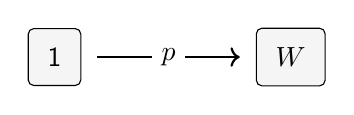
\begin{tikzpicture}
					\node[dpadded] (1) at (0,0) {$\sf 1$};
					\node[dpadded] (W) at (3,0) {$W$};
					
					\draw[arr] (1) to node[fill=white]{$p$} (W);
				\end{tikzpicture}}
			\end{center}
		\end{examplex}
	\end{vleftovers}
%joe4: \end{commentout}
		\item Double-headed arrows, $A \tto
                  B$, which visually indicate the degenerate special
                  case of a cpd that assigns probability 1 to $f(a)$
                  for each $a \in A$ (corresponding to a deterministic
                  function $f : A \to B$). 
	\end{itemize}


%oli11: Easier reference for this construction
\begin{constr}\label{constr:hyperedge-reducton}
We can now explain how we capture   the multi-tailed edges that 
were used in 
\Crefrange{ex:smoking}{ex:grok-union}. 
That notation can be viewed as shorthand for the graph that results by adding a new node at the junction representing the joint value of the nodes at the tails, with projections going back.  For instance,
% the diagram of the PDG in the shaded box of \Cref{subfig:smoking-pdg}
the diagram displaying Grok's prior knowledge in \Cref{ex:grok-union}, on the left of \Cref{fig:grok-combine}
%joe7: moved up from below, to save a line
%is really shorthand for the following PDG:
is really shorthand for the following PDG, where
where we insert a node labeled $C \times T$ at the junction:
	\begin{center}
		\scalebox{0.8}{
		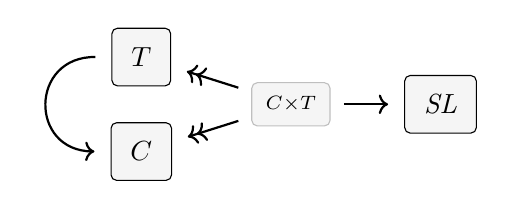
\begin{tikzpicture}
			\node[dpadded] (SL) at (-1.0,0) {$\mathit{SL}$};
			
			\node[dpadded,light pad] (CT) at (-2.9, 0){$\scriptstyle C \times T$};
			\node[dpadded] (C) at (-4.8, -0.6) {$C$};
			\node[dpadded] (T) at (-4.8, 0.6) {$T$};
			
	%				\node[dpadded, dashed,color=violet] (X) at (6.5,0) {$X$};
	%				\draw[arr, color=violet] (X) -- (S);
	%				\draw[arr, color=violet] (X) -- (C);
	%				\draw[arr, dashed, color=violet] (X) -- (SC);
			
			\draw[arr, ->>] (CT) -- (C);
			\draw[arr, ->>] (CT) -- (T);
			\draw[arr] (CT) -- (SL);
			\draw[arr] (T) to [bend right=90, looseness=2] (C);
	\end{tikzpicture}}
	%%%%%%%%%%%%%%%%%  smoking fragment: %%%%%%%%%%%%%%%%%%%%%%
% 		\scalebox{0.8}{
% 			\begin{tikzpicture}
% 				\node[dpadded] (C) at (-1.0,0) {$C$};
% 				\node[dpadded] (T) at (0.5,0) {$T$};
% 
% 				\node[dpadded,light pad] (SSH) at (-2.9, 0){$\scriptsize \mathit{SH} \times S$};
% 				\node[dpadded] (S) at (-4.8, 0.6) {$S$};
% 				\node[dpadded] (SH) at (-5.0, -0.6) {$\mathit{SH}$};
% 
% %				\node[dpadded, dashed,color=violet] (X) at (6.5,0) {$X$};
% %				\draw[arr, color=violet] (X) -- (S);
% %				\draw[arr, color=violet] (X) -- (C);
% %				\draw[arr, dashed, color=violet] (X) -- (SC);
% 
% 				\draw[arr, ->>] (SSH) -- (S);
% 				\draw[arr, ->>] (SSH) -- (SH);
% 				\draw[arr] (SSH) -- (C);
% 				\draw[arr] (T) -- (C);
% 		\end{tikzpicture}}
	\end{center}

% That is, we inserted a node labeled $SH \times S$ at the junction.  As
% the notation suggests, $\V( \mathit{SH} \times S) = \V(\mathit{SH}) \times \V(S)$.
% The cpd for $(h,s) \in \V(\mathit{SH} \times S)$  associated with 
% the edge from $\mathit{SH} \times S$ to $\mathit{SH}$ gives probability 1 to $h$;
% similarly, the cpd for $(s,c)$  associated with 
% the edge from $ C \times C$ to $S$ gives probability 1 to $s$.
%joe7
%        That is, we inserted a node labeled $C \times T$ at the junction.
As the notation suggests, $\V( C \times T) = \V(C) \times \V(T)$.
%joe2: this is not the time to start talking about matri\mathit{SL}es
%Thus, $\V(S \times \mathit{SL}) = \V(S) \times \V(\mathit{SL})$; the matrix asso\mathit{SL}iated with
For any joint setting $(c,t) \in \V(C \times T)$ of both variables, the cpd for
the edge from $C \times T$ to $C$ gives probability 1 to $c$;
similarly, the cpd for the edge from $ C \times T$ to $T$ gives probability 1 to $t$.
\end{constr}

%oli11: Quickly hint about why this works syntactically, so we can
%better summarize this contribution
%joe10*: NO!!!  This ha nothing to do with our story, It's a complete
%distraction.  I don't see the connection between a failure of
%consistency and a failure to commute (and I have a Ph.D. in
%mathematics and no exactly what the words mean).  I *strongly* object
%to including this.  If you have some interesting theorems to prove,
%you can write another paper on it.  You can also talk about it in
%your thesis if you really care.  But not in the paper!  Even if we
%could afford the space (which we can't) I would strongly object.
%oli12*: Are you serious that you don't see the connection?? We should
%talk about this.
%joe11: Yes, I'm serious.  We can discuss it after the deadline.
% I really do think it's a massive oversight not to at least mention
% this. I can see a world where mentioning this is the most important
% thing we do in the paper. I also think you hugely underestimate how
% many people care about commutative diagrams, what this buys you, and
% the implications for mathematical reasonsing.
%joe11: There are certainly people who care about this material.  They
%are an extremely small subset of the NeurIPS community.  We're
%submitting this paper to NeurIPS.  You're more than welcome to write
%a paper about this for a conference where there are substantially more pepole
%who care about commutative diagrms.
\begin{vfull}
    We have stressed that edges are interpreted differently in PDGs than
    in Bayesian Networks. Readers should be aware that this approach is
    closely related to the notion of a \emph{commutative diagram}, a
    common representation in pure mathematics. For those familiar with
    them, the potential failure of a PDG to be consistent is analogous to
    the possibility that a diagram could fail to commute. 
\end{vfull}

%joe4*: cut this paragraph.  It's a distraction.  Moreover, BN's don't
%need this ``trick'', because of the way they interpret the edges.  
\commentout{
This trick will not work for a BN. We need cpds to be associated with
edges, so that the projections do not get in the way of the other
information we would like to encode. In this case, we would like to
give some probabilistic information on the edge from $T$ to $C$, but
if we think of this picture as representing a BN, then $C$ would
require a table for joint settings of $(C \times T, T)$. The only
reasonable way to provide this cpd is to ignore the second component,
and use the value of $c$ determined by $C \times T$---which clearly
has no more information than the projection itself.     
}
\commentout{
	We can also generalize PDGs by associating with each edge $L$
        two additional parameters, a confidence $\beta_L \in [0,
          \infty)$, which can be viewed as indicating the strength of
          the belief that the cpd attached to $L$ is correct, and a
%joe5: I don't understand your intuition behind ``degree of
%causality'', and really don't like that name.  Is it standard?  
%oli6: It's not standard. It is a knob one might want to turn,
%effectively controls how important it is to preserve the cpd
%counter-factually, and my limited experience playing with it suggests
%that it lines up with other causal intuitions. Other suggestions for
%terminology are appreciated.
%joe6: I can't suggest good terminology for a notion I don't
%understand. But you definitely should avoid notation that suggests
%inappropriate connections.  I would have called ``degree of
%causality'' as the extent to which a is a cause of b.  That would
%make it somewhat related to what Hana Chockler and I called the
%degree of responsibility.  But I don't think that that's what you had
%in mind at all. 
          degree of causality $\alpha_L \in [0,1]$, which indicates
          the degree to which this cpd should be trusted if the
          distribution at its source were to change: 

	$\alpha_L = 0$ corresponds to a conditional observation that
          one does not necessarily believe will generalize, and
          $\alpha_L = 1$ corresponds to a belief that there is a real
          mechanism with the same underlying direction of dependence.  
	As we will see in \Cref{ex:alpha-motivation}, this difference
        should change our calculus for approximating a PDG with a
        distribution, and will be a crucial point of distinction
        between a BN and a factor graph. 
%In particular, for each edge $L \in \Ed$, we associate two real parameters $\beta_L, \alpha_L$ indicating the certainty in a belief, its degree of causality, respectively. 


	\begin{example}\label{ex:alpha-motivation}
		Suppose $\V(X) = \{x_0, x_1\}$ and $\V(Y) = \{y_0,
%joe6: corected typo, on the off chance that this stays somewhere.
%                \ldots, y_100\}$, and consider the cpd $\mat p$
                \ldots, y_{100}\}$, and consider the cpd $\mat p$
                associated with an edge from $X$ to $Y$: 
		
		\begin{equation}
			\bp(x) = \begin{cases}
				\mathit{Uniform}_Y & x = x_0 \\
				\delta_{y, y_7} & x = x_1
			\end{cases}
		\end{equation}

		For instance, Grok starts to notice that there is a letter in her mailbox ($X = x_1$), then her neighbor always has the same letter in his mailbox ($Y = y_7$). If Grok has no letters ($X = x_2$), her neighbor has a one of many letters (Grok has been keeping track of the distribution, which is nearly uniform)
		
		You have no idea how often or Grok gets letters or why. Which of the following intuitively seems to be a more likely marginals on Grok and her neighbor's letters?
		
		\begin{enumerate}
			\item She get a letter with 50/50 probability, and her neighbor gets a particular one with 50\% probability, and others with small, equal probabilities which add to 50\%. \label{item:unifprior}
			\item Grok is much more likely not to get a letter, and her neighbor gets one of 100 letters with roughly uniform probability. \label{item:infoprior}
		\end{enumerate}
		 	
				
		Though we could tell other stories with the same cpd,
                where (\ref{item:unifprior}) feels more appropriate,
                in this case it seems natural to conclude that option
                (\ref{item:infoprior}) is more reasonable. The reason
                is that the difference in information between the two
                settings is very large. If have no a priori reason to
                think one world is more likely than another, then with
                this constraint, there are 100 possible worlds where
                 $X = x_1$ and only one where $X = x_0$. Thinking that
                (\ref{item:infoprior}) is more appropriate corresponds
                to calculating the distribution of maximum entropy
                satisfying the cpd, thought of as a constraint. The
                larger the number of possible values of $Y$, the
                smaller the intuitive value of $\alpha$. 

		
		On the other hand, thinking that (\ref{item:unifprior}) is more appropriate corresponds to the causal view: in this case we start by acknowledging we know noting about $X$ and therefore assigning it the maximum entropy distribution, and then asserting that . This is roughly equivalent to asserting that $\mat p$ holds counterfactually, independent of the distribution on $X$. 
	\end{example}
	
	We therefore adopt the following definition, with both $\alpha$ and $\beta$ parameters:

	\begin{defn}
		A weighted PDG $(\dg M, \vec \beta, \vec \alpha)$ is a PDG
	%joe4*: I would replace ``certainty'' by ``confidence''.  If you want
	%to include what you're calling ``degree of causality'' as well, you
	%*must* give some intuition here.  It can't come out of the blue.  You
	%don't have to go into detail, but you have to say something.  I have no
	%clue what it reprsents.
	%oli5: I've added more context above, and an example below.
	        $\dg M$ together with a \emph{confidence} $\beta_L \in \mathbb
	        R^{\geq 0}$ and \emph{degree of causality} $\alpha_L \in
	        [0,1]$ for each edge $L \in \Ed^\dg M$. 
	\end{defn}

	We identify an unweighted PDG with a weighted PDG where $\alpha_L
	= \beta_L = 1$ for each edge $L$.
}
\section{PDGs: Semantics}\label{sec:semantics}
%oli12: I dislike the sentence below. Primarily, it seems like
%cheating to come up 
% with totally different semantics depending on what you want to capture, and 
% we're really not doing that --- our three semantics are intimately
% related, and 
% can all be represented naturally in terms of the scoring function. 
%   There is more than one way of giving semantics to a PDG.  
%oli12: I think something along these lines has the additional benefit of 
% quickly speaking to why we're doing this (people write down cpds all the time). 
Although the meaning of an individual cpd is clear, we have not yet given 
%joe11: you seem to like using ``local'' and ``global'' a lot.
%Although I understand what you intend here, I'm still uncomfortable
%about the usage, because it suggests that there's a local semantics.
%oli13: There is a local semantics: the cpd itself already is a local
%probabilistic object. It is already useful on its own. You can even compose
%them, etc,... But there's ambiguity in stitching them together. In some sense
%this is the problem we address.
%joe12: but we have never talked about local semanatics or local
%probabilistic objects.  This is not the time to start!
%oli14: Anecdotally, this is the point that convinced me that semantics was 
% actually worthwhile. Many people just use cpds by themselves; I'd guess many
% ML people will be wondering why we need anything else if we already have
% the cpds that we need. Can't you just do math with those? In any
% case, "global" 
% is good enough for me.
%joe11: I left it in with the quotation marks.
%oli13: The "local" and "global" is going to also help make sure these terms
% don't come out of the blue later in the paper.
%joe12: but they come out of the blue here.  Do we really need them?
%Are they adding something useful to the discussion?  (As you can
%guess, I don't think that they do.)
%oli14: I think they are. I think this "global" here is already worth it
% even if we don't follow up. I have plenty of following up to do, but
% probably anything substantive won't make it. I have just a few
% characters on the final page. 
%PDGs any global semantics. We discuss three related approaches. The first
%joe14
%PDGs a ``global'' semantics. We discuss three related approaches. The
PDGs a ``global'' semantics. We discuss three related approaches to
doing so. The
first 
is the 
simplest: we associate with a PDG the set of distributions that are consistent
with it. This set will be empty if the PDG is inconsistent.
%
The second approach associates a PDG with a scoring function, indicating the fit
of an arbitrary distribution $\mu$, and can be thought of as a \emph{weighted}
set of distributions \cite{HL12}. This approach allows us to distinguish
inconsistent PDGs, while the first approach does not. The third approach chooses
the distributions with the best score, typically associating with a PDG a unique
distribution.

\subsection{PDGs As Sets Of Distributions}\label{sec:set-of-distribution-semantics} 
We have been thinking of a PDG as a collection of constraints on distributions, specified by matching cpds. From this perspective, 
%oli12
% a natural thing to consider is 
it is natural to consider
the set of all distributions that are consistent with the constraints.

\begin{defn} \label{def:set-semantics} 
If $\dg M\sheq\pdgvars[]$ is a PDG, let $\SD{\dg M}$ be the \emph{s}et of \emph{d}istributions over the variables in $\dg M$ 
%oli12: "the conditional probabilities" is ambiguous, I thought it was reffering
%to p. For a joint distribution p, it's the conditional _marginal_ on the
%appropriate variables that's of interest.
% for which the conditional probabilities are exactly 
%joe11
%whose conditional marginals on are exactly those given by $\mat p$.
whose conditional marginals are exactly those given by $\mat p$.
That is, $\mu \in \SD{\dg M}$ iff, for all edges $L = (X,Y) \in \Ed$,  $x \in \V(X)$,  and $y \in \V(Y)$, we have that $\mu(Y = \cdot \mid X\sheq x) = \bp(x)$.
\notation{Formally,		
        \[ \SD[\Big]\dg M = \!\left\{\mu \!\in\! \Delta \V_\none (\dg M) \middle|\!
        \begin{array}{l}
        \mu(B\!\! =\!\!b \mid A\!\!=\!\!a) \geq \boldsymbol\mu_L(b \mid a) \\[0.1em]
        ~\text{$\forall (A, B,\ell) \!\in\! \Ed$, $a \!\in\!\mathcal V_A$, $b \!\in\! \mathcal V_B$} \end{array}\!\!\! \right\}\]
    }
%oli12: while I still prefer and would prefer to promote 'inhabited'
%(no negatives), I think we can agree that a single negative is easier
%to follow single negative than tripple negative.
%joe11: I have a slight preference for the original was fine, but I
%don't feel strongly enough about it to override the change.
%oli13: Maybe more equitible emphasis will help...
% $\dg M$ is \emph{consistent} if $\SD{\dg M} \ne \emptyset$, and inconsistent otherwise.
% $\dg M$ is \emph{inconsistent} if $\SD{\dg M} = \emptyset$, and consistent otherwise.
$\dg M$ is \emph{inconsistent} if $\SD{\dg M} = \emptyset$, and \emph{consistent} otherwise.
\end{defn}

	\begin{vfull}
		It turns out that this semantics only results in convex sets. This may provide useful intuition, and we will prove a stronger version of this statement that corresponds to our second semantics.
		\begin{lemma}[restate=thmsetconvex] 
			\label{prop:convex}
			$\SD{\dg M}$ is convex, for any PDG $\dg M$.
		\end{lemma}
	
		Note that being inconsistent is not the same things as \emph{over-constrained}: 	
		\begin{defn}
			$\dg M = \pdgvars[]$ is over-constrained if there exists
			  \emph{some $\mat p'$} assigning cpds to the same edges as
			  $\mat p$, such that $(\N, \Ed, \V, \mat p')$ is inconsistent
			  \notation{(i.e., $\SD{\N^\dg M, \Ed^\dg M, \V^\dg M, \mat p}
				= \emptyset$)}, and under-constrained if there are
			  multiple distributions in $(\N, \Ed, \V, \mat p')$ for
			  \emph{every such $\mat p'$}, making this a property of the
			  qualitative PDG $(\N, \Ed, \V)$.  
		\end{defn}

		We know that an under-constrained PDG is consistent without even looking at the tables. However if a we know that an \emph{over-constrained} PDG is actually consistent (when it could have easily contradicted itself), the information provides corroborating evidence, and one can take this as support in favor of the beliefs. 
	\end{vfull}
        
%joe3        
        %	\subsection{PDG S AS WEIGHTED
%joe7
        %	\subsection{PDGs As Distribution Scorings}
%oli12: You seem insistant on this particular heading; but here's why
%it bugs me: 
% This suggests linguistically that we interpret a PDG as the score of one (or many) of distributions, but in fact it's only the scoring _function_.  
%joe11: I can live with this
        % \subsection{PDGs As Scores of Distributions}
\subsection{PDGs As Distribution Scoring Functions}
\label{sec:scoring-semantics}   
We now generalize the previous semantics by viewing a PDG $\dg M$ as
a \emph{scoring function} that, given an arbitrary distribution $\mu$ on $\V(\dg M)$, 
returns a real-valued score indicating how 
%oli12
%joe11: I definitely prefer the original; why did you make the change?
%oli13: To emphasize the polarity. I'm willing to cede here, but technically
% Inc is a measure of poorness of fit, not goodness of fit; the other is more 
% in both respects. 
%joe12: undid; I don't see why Inc is a measure of poorness rather than
%goodness of fit.
%oli14: At the risk of pointing out the obvious, it's only bound (a perfect score)
% is when there's nothing wrong, and it only gets worse. But I'm sure you know this
% so I won't change it.
well
%poorly
$\mu$ fits $\dg M$. Distributions with the lowest (best) scores are those that
most closely match the cpds in $\dg M$, and contain the fewest unspecified correlations.
%oli12: we've used this transition several times now. I think it flows
%fine without it. Removing 
	% We now make this precise.

We start with the first component of the score, which assigns higher scores to distributions that require a larger perturbation in order to be consistent with $\dg M$.  
%oli12: Do you still think (as below) that referencing an example is
%appropriate?
%joe11: while I don't think it's critical for the 8-page abstract, I
%do think it would be nice to have an example showing ``this
%distribution is more inconsistent with the PDG than that one''.  It
%can just  be a brief example, done in one sentence. I'm not thinking
%of something elaborate with a diagram.
%joe3*: It would be good to have an example of degrees of
%inconsistency here, before we give them a score.  One of the
%xamles from the intro would work, with variants of the cpd making it
%more or less consistent.
We measure the magnitude of this perturbation with relative entropy. In particular, for each edge $L = (X,Y, \ell)$, and each $x \in \V(X)$, we measure the relative entropy from $\bp(x)$ to $\mu(Y \!= \cdot\mid X=x)$, take the expectation over $\mu_X$ (that is, the marginal of $\mu$ on $X$). We then sum over all the edges $L$ in the PDG, weighted by their reliability.


\begin{defn}\label{def:inc}
	The \emph{incompatibility} of a PDG $\dg M = \pdgvars[]$ with
	a joint distribution $\mu$, denoted $\Inc_{\dg M}(\mu)$, is  
    \[
	\Inc_{\dg M }( \mu) := 
		\!\!\!\sum \alle \beta_L \E_{x \sim \mu_{_X}}
            \left[\kldiv[\Big]{ \mu(Y\!= \cdot\mid X \sheq x) }{\bp(x) } \right] ,
	\]
	where $\kldiv{\mu}{\nu} = \sum_{w \in \text{Supp($\mu$)}} \mu(w) \log\frac{\mu(w)}{\nu(w)}$ is the 
	relative entropy from $\nu$ to $\mu$.
\begin{vfull}
The \emph{inconsistency of PDG $\dg M = \pdgvars[]$}, 
       denoted $\Inc(\dg M)$, is the
minimum possible incompatibility of $\dg M$ with any
distribution $\mu$,  
	\[ \Inc(\dg M) = \inf_{ \mu \in \Delta [W_{\cal V}]} \Inc_{\dg M}(\mu) . \]
\end{vfull}
%joe4: It would be useful to have a marker for the end of the
%definition.  I'm not a big fan of the triangle marker that you used
%before (and it's quite nonstandard).
%oli12: As you've probably noticed, I added a diamond marker to the definitions.
% I do not care at all what markers are used (though squares mean QED
% to me, and hence seem weird for examples / definitions) --- you can
% change both markers to whatever you want by searching for
% "\declaretheorem" and then changint the "qed=" field.
%joe11: I prefer squares; I find the diamond a bitoff-putting,
%although I can't explain why.  Squares are definitely more standard
\end{defn}

\begin{vfull}
The idea behind this definition of inconsistency is that we want to choose a
distribution $\mu$ that minimizes the total number of bits required to encode
all of the relevant conditional marginals. More precisely, fix a distribution
$\mu$. For each edge $L = (X, Y,
%joe4* Please address the %joe3 comment below (and remove the label)
%joe3: Where is the optimal code that we are supposedly given?
%oli5: I don't understand this complaint either. The code might be a
%complicated object 
% and its details don't matter---what matters is that if it's
% optimized to transmit samples from the model, then using it on
% samples generated from a distribution will be less efficient (longer
% code words for things that were thought to be infrequent, end up
        % being used more frequently). What do you mean by where?
%joe5*: My problem is that I have no clue of what you're talking about.
%(Well, that's not completely true, since I've seen some of the
%connection of entropy to codes before. But for those who haven't seen
%it, or haven't really absorbed it -- which includes me -- this is
%comletely mysterious.  You start talking about optimal codes that we
%are ``given'', and I have no idea what this is
%joe6*: what is a code for Y?  
%oli7*: It is an encoding of the values of $Y$ as sequences of bits.
% A code that is  "optimal for a distribution \mu" is one for which 
% the expected number of bits of a sample of Y, drawn from \mu, is minimal.  
        %        \ell) \in \Ed$ and $x \in \V(X)$ we are given a code
\ell) \in \Ed$ and $x \in \V(X)$, we are given a code for $Y$ optimized for the
distribution $\bp(x)$, and asked to transmit
%joe6: I would expect the cost to involve a difference between two
%quantities, but the formal expression doesn't seem to involve a difference.
%There is a difference in the defintion of ``extra information''
%below.  So perhaps this explnation is premature.  
%oli7: the definition of relative entropy has a log of a ratio; expanding it 
% results in the diference you're looking for.
data from $\mu(Y\mid x)$; we incur a cost for each bit required beyond what we
would have used had we used a code optimized for the actual distribution
$\mu(Y\mid X=x)$. To obtain the cost for $L$, we take a weighted average of
these costs, where the weight for the value $x$ is the probability $\mu_X(x)$.
We do this for every edge $L \in \Ed$, summing the cost.

For even more intuition, imagine two agents ($A$ and $B$) with identical beliefs described by a PDG $\dg M$ about a set of variables that are in fact distributed according to $\mu$. For each edge $L = (X,Y, \ell) \in \Ed^\dg M$, values $x,y \in \V(X)$ are chosen according to $\mu_{_{XY}}$ and $x$ is given to both agents. 

At this point, the agents, having the same conditional beliefs, and
the same information about $Y$, agree on the optimal encoding 
of the possible values of $Y$ as sequences of bits, so that if $y$
were drawn from $\bp(x)$, the fewest number of bits would be needed
to communicate it in expectation. The value of $y$---which is distributed
not according to $\bp(x)$, but $\mu(Y \mid X=x)$---is now given to agent A.
The agents pay a cost equal the number of bits needed to encode $y$ according
to the agreed-upon optimal code, but reimbursed the (smaller) cost that would have been paid,
had the agents beliefs lined up with the true distribution $\mu$.

Repeating for each edge and summing the expectations of these costs, we can view
$\Inc_{\dg M}(\mu)$ as the total number of \emph{additional} expected
bits required to communicate $y$ with a code optimized for
$\bp$ instead of the true conditional distribution   $\mu(Y \mid X=x)$. 

If $\dg M$ is inconsistent, then there will be a cost no matter what distribution $\mu$ is the true distribution. Conversely, if $\dg M$ is consistent, then any distribution $\mu \in \SD{\dg M}$ will have $\Inc_{\dg M}( \mu) = 0$.  
\begin{example}[continues=ex:worldsonly]
Recall our simplest example, which directly encodes an entire distribution $p$
over the set $W$. In this case, there is only one edge, the expectation is over
a single element, and the marginal on $W$ is the entire distribution. Therefore,
$\Inc(\dg M; \mu) = \kldiv{\mu}{\mu}$, so the inconsistency is just the
information $\mu$ and $p$, so is minimized uniquely when $\mu$ is $p$
\end{example}
%
\end{vfull}
	
$\SD{\dg M}$ and $\Inc_{\dg M}$ distinguish only
between distributions based on their compatibility with
$\dg M$, but even among distributions that match the
marginals, some more closely match the qualitative structure
of the graph than others.  
\commentout{
Suppose an agent has a PDG $\dg M$ in mind, and imagines that all sample
variation in a joint distribution $\mu$ over $\V(\dg M)$ arises as a result
%joe9*: In the next line, did you mean ``some'' or ``each''? See my
%next joe9*
%oli11: Both words are ambiguous because of the sentence structure,
%but I meant to say that we imagine the distribution is generated by
%rolling the dice in each link. What we do is clear from the
%formula. I think this is why I prefer putting the formula before the
%explanation --- people read the explanation already knowing what
%you're going to do, and then learn why you do it.
%joe10: there are reasons to put intuition before the formula, and
%reasons to put after.  I generally prefer giving a high-level
%intuition first, and then following up with more intuition after the
%formula if it's would help                
of sampling the value of a target variable $Y$ of some edge $\ed LXY$, given the
value of $X$. If this is the case, one would expect the total amount of
information required to communicate a sample of $\mu$ to be the same as the
total amount of the information required to separately encode, for
each edge $\ed LXY$, the randomness of $Y$ given $X$.

For an arbitrary PDG and $\mu$, these two quantities will differ; if the amount
of uncertainty in the distribution is lower than one would expect from the
edges, the distribution has an \emph{information deficiency}, indicating that there
are additional correlations between variables that are not captured by the
graph. The higher the information deficiency, the worse the qualitative fit between
the PDG and $\mu$.
%joe9*: Now you lost me.  What is ``surplus uncertainty''? This needs
%tob e given *much* more intuition.
On the other hand, if a distribution has surplus uncertainty, using it confers a
benefit. For instance, a PDG containing only the variable $X$
%joe9* I strenously object to the use of ``safest'' in the way you've
%used it below.  What is safe depends on utilities, which we haven't
%mentioned. 
%oli11: I think this is false. While to express "safe" in general, you
%would need a utility function, I claim that there is not *any*
%utility function that, over the joint space of random variables here,
%would change this calculus at all (except to make it so that you
                %don't care).
%joe11: I dsagree; you're too wedded to maxent.  But this is not the
%time to have this battle                
% there's 
%oli13: (This part is still commented out.)
%joe12: good; let's keep it that way :-)
and no
edges encodes awareness about $X$ but no beliefs about it. Given that $X$
could be distributed in any way (even chosen adversarially), it is safest to act
as though you believed $X$ to be uniform.  
%oli11: irrelevant because commented out anyway, but I think what I
%wrote is more coherent than the below.  and no edges leading to $X$
%means that the agent is  aware of $X$, but has no  information
%regarding the probability of various values of $X$ but no 
We measure the surplus/deficit with a quantity we call
the \emph{information fit} ($\IDef$) (between ${\dg M}$ and $\mu$):
}
%oli11: end comment. The summary at the end of our meeting was,
%" Given a distribution, compare the cost of specifying \mu directly
%to the cost of specifying the information on the edges for \mu.". You
%also said not to say anything about samples, but it's information
%required to specify a sample of the distribution, given the
%distribution. I'll try a slightly different appraoch, but I don't
%have a good idea about what's going to stick. 
%Let $G$ be a (multi-)graph whose nodes correspond to random variables. 
%joe10
%Each edge $\ed LXY$ of a PDG $\dg M$ represents a qualitative claim
We think of each edge $\ed LXY$ of a PDG $\dg M$ as representing a
qualitative claim that the value of $Y$ can be (noisily) computed from
$X$ alone.  
%
%joe10*: I'm not happy about his, because ``amount of variation'' is
%not well defined. Whateever intuitions you're suggesting here is (in
%my opinion) too closely tied to entroyp.  As a technical matter, I
%think you want to talk about \mu matching \dg M.  Also, in fact, it
%does not match the definition, since it doesn't say what to do with
%parallel edges
%oli13: We already talk about matching in the sentence above.
%oli13: ALso the parallel edges is the reverse of what I'm talking about here.
%How do I people from getting this mixed up? If you think about it carefully.
%With parallel edges (b) > (a) and as we've said, there are additional
%correlations that allow for a more  compact representation. That's the case
%that parallel edges push towards ( and of course the total score is just in
%net). We still need to give intuition for the other case though; here we need
%to say something about the case when (for instance) there are no edges at all.
%joe12: I didn't understand what you wrote above
%   A joint distribution that qualitatively matches $\mu$ will intuitively
%   have as much variation as possible, except where we have claimed that
%   one variable depends on another.
%oli13*: Ok, but we need to impart slightly more detailed intuition instead of
% saying this. I know you don't like entroyp, but given that our formua uses
% entropy (Sorry), and we need to  say something of intermediate formality here
% that gives the right intuition --- we need to say something about variation, 
% or something else that's equivalent with different words. That's the 
% concept we need to communicate here. It doesn't matter if it's undefined, we
% are about to define it. You do a good job explaining it. We'll explain it 
% eve more carefully in the appendix. I promise you nobody at Neurips will care.
% People take so much information theory (and whatever else) for granted; for 
% the full paper, I think we can say enough to make you happy, because I belive
% it really is well-motivated.
%joe12: sometimes less is more.  If you can impart useful intuition.
%oli14: THe reason I keep changing your words in this particular
%section is not 
% because I don't like the way they sound, but because I think they either say
% almost nothing, or they are slightly wrong / misleading. Considering the 
% (perhaps regretably) standard % culture of talking in a cavalier way about
% information, I think I have a bit better sense of how to impart useful
% intuition about entropy.
%I'd *strongly* prefer to say something well in the appendix and nothing
%here rather than saying something not-so-good or unclear here.   
%that's good.  If what you impart is not so useful, then not so good.
%oli13: The current sentence does not serve the correct purpose (and its purpose has
% alredy been fulfilled by the first sentence in the paragraph).
% Thus, given ${\dg M}$, for each measure $\mu$, we consider how well
% the structure of ${\dg M}$ matches that of $\mu$.
%oli14*: I actually really like this sentence, save for the word "anything" 
% (which may be replacable but I could not do easily without either
% being more vague or 
% technical than is your standard preference)
% Think about it carefully before you change it. 
    % The best description of an outcome drawn from a joint distribution that 
%oli16: deleting entire sentence, starting over below.
%joe13
%qualitatively matches $G$, should intuitively both be efficiently
    % qualitatively matches $G$ should intuitively both be efficiently
%oli16
    % described by $G$
    % wherever $G$ has an edge,
%oli16: I'm not super happy with the two lines above either.  line below added
% and then removed.
% described by the conditional outcomes of each edge of $G$,
%joe13
%while also encoding uncertainty about
%oli15: it's not just dependence--- it's technically not accurate
%because there's also the univariate case! 
% while also not having dependences between variables where there is
% no edge in $G$.
%joe14*: Sorry; I do not understand ``maximal information'' in the next
%line.   %This has to be rewritten.  My preference would be for
%reinstating what I wrote.   I don't understand the issue with the
%univariate case, and evenif there is an issue with the univariate
%case, it doesn't prevent what I wrote from being good intuition.
%oli16: the problem is that   
% while also being requiring maximal information to encode relationships
% not in $G$ [[REWRITE]]. 
%oli16: It's so very difficult to write this sentence without making
%it technical, talking 
% about information, or lying....
%oli16: What I had before:
    % The best description of an outcomedrawn from a joint
    % distribution that qualitatively matches $G$ should intuitively
    % both be efficiently described by $G$ wherever $G$ has an edge,
    % while also requiring maximal information to encode relationships
    % not in $G$. 
%oli16: I did a bunch of rewrites, and kept the last 4 in the comments below.
%oli16:rewrite 1:
    % A distribution $\mu$  qualitatively matches $G$ well if it is
    % efficient to describe the outcomes along the edges of $G$, but
    % hard to describe features of $\mu$ that are not encoded by the
    % edges of $\mu$.  
%oli16:rewrite 2:
% pros: no lies, short, should be reasonable intuition. 
% cons: "respect" and "relationships" are vague.
%joe15: this didn't help at all.  I don't understand what it means to
%be ``inefficient to describe''.  It's OK to lie a little when giving
%intuition.  We said above than an think of edge from X to Y as
%''representing a qualitative claim that the value of $Y$ can be
%(noisily) computed from $X$ alone.'' If you want to say something about
%non-edges, it should be that there is no edge from X to Y if we can't
%compute X from Y alone.  If you think that's not quite right, then
%it's better to say nothing than to say something which is likely to
%confuse the reader, especially given how we've described the meaning
%of an edge.
%oli17: I don't think that saying that helps bridge the gap between this idea
%and the next one. I am willing to settle with the document in its current
%state. However, if you read these two paragraphs again closely, you will see
%a rather large chasm between the "qualitatively described just by X" bit, and
%the "information requird to draw a sample" bit. We do not explain why they are
%related. We might modify the first part, but we cannot delete it because we
%need to talk about the qualitative nature of a link; I think that changing the
%secong part significantly is an even bigger mistake, as this is the best
%intuition we give for the equation.
%
%$G$ should be inefficient to describe in every respect except those
%relationships that are encoded by the edges of $G$.  
%oli16:rewrite 3:
% pros: technically accurate
% cons: not the clearest why this is desirable. 
    % We judge a distribution $\mu$ to qualitatively fit $G$ better
    % when the features of an outcome $\mat w \sim \mu$ that follow
    % from the conditional outcomes of $G$ are easy to describe (given
    % $\mu$), and worse when any other features (i.e., those not
    % described by $G$) of $\mat w$ are easy to describe (given
    % $\mu$). 
%oli16:rewrite 4:
% pros: still accurate, more explicit about why it works
% cons: not very eloquent, and might require some of the figures to
% really see why this is the same as the formalism. 
    % Intuitively, a distribution is most likely to have been
    % generated by the edges of $G$ if the information required to
    % specify a the target variables of $G$ directly is no more than
    % the information required to sample separately along the edges of
    % $G$. If $\mu$ makes it easy to describe other aspects of a
    % sample, that $G$ does not articulate, this counts against the
    % match, because we imagine that $G$ would have included these
    % edges if they were easy to communicate qualitatively. 
%oli13: This "anything" is intentionally vague. We cannot clarify this with 
% just the variables it says nothing about, because cycles are possible. 
%joe12*: NO!  I don't know what it means, and I won't accept vagueness
%here.  It's better to cut it!  I need to go now; I'll come back to
%this around 2.
%oli14: Ok, I'll try something slightly less vague.
% anything
%joe13: cut
%\todo{anything}
%that is not described by $G$.
%joe10
%To formalize this, we require only the underlying multigraph $G :=
To formalize this, we require only the underlying multigraph $G^{\dg M} :=
(\N^{\dg M}, \Ed^{\dg M})$ of $\dg M$. 
%joe10: I'm not ure where there ``are known'' is coming from
%oli12: I don't think this is strictly necessary, but it could be useful
% clarification. It seems you (and sometimes I) sometimes get
% mixed up about what exactly this information means.
% The point is that it's the information needed to specify
% the outcome if you already know it is drawn from \mu. 
%joe11: the sentence with ``are known'' doesn't even parse.  Let's
%just leave it.
%oli13: Oops, this parses though (I don't think the "we thus" buys us anything except fluff):
%joe13: whether or not \mu is known is irrelevant!  Why empahsize it
%For a fixed $G$ and known $\mu$, contrast the amount
%oli15: very false. \mu has to be common knowledge! I won't change
%joe14: knowledge has nothing to do with anything here!  There are no
%agents in the picture in this definition.
%oli16: We're now heavily leaning on the term "description", which I argue
% is effectively knowledge. As a technical matter, the way we
% calculate the length of this  
% description assumes that the distribution \mu is known to both the
% sender and reiever of the description.
%joe15: I don't see why.  A calculation is a mathematical expression.
%At best you can say that they way you *use* the result of the calculation is
%meaningful only if something is common knowledge,  but that would
%depend on the usage.   The calculation itself does not depend on
%knowledge. There is no sender and receiver anywhere in our formalism.
%oli17: Ok no more agentive terminology. For the  "description" metaphor to make
%sense, it's necessary that the description gets to exploit the distribution.
%Therefore both the construction of the description, and the interpretation of
%the description, must depend on \mu. Are we now on the same page?
%joe16: I'm afraid not.  I'm not sure what you mean by ``the
%interpretation of the description'' and how ``the construction of the
%desription'' differs from ``the description''.  I'm happy to agree
%that everything (whatever everything is) depends on \mu.
Given $G$ and $\mu$, contrast the amount of
%For an arbitrary  $G$ and $\mu$ are known, contrast the amount of
% We thus consider the difference between the
information required to 
\begin{enumerate}[label=(\alph*)]
\item directly describe a joint outcome  $\mat w ~ \sim \mu$
          drawn from $\mu$, and 
	\item separately specify, for each edge $\ed LXY$, the value
%joe10
%          $\mat w_Y$  given the value $\mat w_X$, in expectation. 
          $\mat w_Y$ (the projection of $\mat w$ onto the variable
          $Y$) given the value $\mat w_X$, in expectation. 
\end{enumerate}
% (a)  and (b)
When these two quantities are equal,
%joe11: let's leave agents out of it
%an agent that
%oli12: reword
% is prepared to specify 
%is prepared to recieve
%(b) is expecting a description of exactly the same length as
%oli13: deleted
%then
a specification of
%oli13 deleted
% the form 
(b) has exactly the same length as
%joe12: describe a full description
%oli14: i.e., the number of bits required in expectation to
%communicate an entire
%joe13: you misudeerstood the previous comment.  it was what was in
%the text before.  I commented it out.  
% sample from \mu, if \mu is common knowledge.
%the one required to describe a full desciption of the world.
a full desciption of the world.
%joe10: misplaced  
%In particular, this is true if
%$\mu$ is a degenerate distribution, in which case the agent, who knows
%$\mu$, requires no descriptions at all.  
%joe10*: Your definition of (b) > (a) seems to me to be identical to
%your eplanation of (a) > (b).  I thin the former is wrong.
%oli12*: Below I wrote
% "there are extra correlations in \mu not described by G" which is the
% exact opposite of "extra dependences in G that are not described by \mu"
%joe11*: I don't understand your sentence above.  If there are
%correlations, then there must be dependencies.  
%oli13: I... think we might be on the same page? The implication is reversed
% in the two quoted phrases.
%oli12: The former is correct, because Entropy measures uncertainty, not dependence.
% also "dependence" of a distribution is undefined, which is why I write
% "correlations". Reverting, because the focus is wrong. It's about \mu, not G
%
%
%If (b) $>$ (a), then there are extra correlations in $\mu$ that are
% If (b) $>$ (a), then there are dependencies suggested by $G$ that are
% not present in $\mu$
%oli12: This special case is not qualitatively different from the one where
% two different edges X -> Y  and  Y <- Z
% , or there may be parallel edges in $G$ (since it is a multigraph) 
% that represent dependencies redundantly.  
%oli12: More importantly, as you've stated yourself, we view G as fixed and correct, for the purposes of evaluating \mu. So saying "if there are parallel edges" is not helpful for talking about \mu. 
If (b) $>$ (a), then there are correlations in $\mu$ that allow for a more
%joe11: I don't kno what ``compressible structure'' means, and I don't
%think we need the addition
%compressed representation than $G$ provides, indicating that $\mu$ has
%more, or qualitatively different, compressible structure than the
%agent expects.
compact representation than $G$ provides.
%oli12: inserted
%joe11: I *really* don't like this.  What does favoriability have to
%do with anything.  Let's leave the agent out of it.
%oli13*: I'm happy to leave an agent out of it, but we still need to indicate
% the polarity of goodness vs badness of fit. I thought you were using the
% agent to tell a story.  Currently the "on the one hand" doesn't have a story.
% We gotta just give the "and so bad fit!" punchline.
The larger the difference, the poorer the fit.
%joe13: in what sense is this true?  Why do we need to say it?
%$\mu$ has an information deficit.  
%The more (b) exceeds (a), the less favorably an agent who believes $G$
%to be correct will view $\mu$.
On the other hand, if (a) $>$ (b), then
%You're still thinking of it (or at least writing it) backwards,
%perhaps because we still don't have "known"! You don't specify \mu,
%but a sample from \mu.
    % $\mu$ requires additional information to specify, beyond
%joe13
%a sample of
$\mu$ requires additional information to specify, beyond
%joe11: G doesn't make claims
%any claims that $G$ makes.
%oli13: let's be more precise 
% what is specified by the structure of $G$.
%joe13*: I don't see any way it which the word ``surplus'' makes sense
%here.  I cut this.  It certainly hurts more than it helps.
%what could be used to encode outcomes of the marginals selected by $G$;
%$\mu$ now has a $G$-information \emph{surplus}.
what could be used to encode outcomes of the marginals selected by $G$.
%$\mu$ now has a $G$-information \emph{surplus}.
%joe11*: I don't like this, and don't really understand it.  Why are
%we suddenly making things  unspecified by G constants.  I cut it.
%oli13: We're not imposing this; I'm just looking at a class of instances, and 
% I think particular class could really help clarify why we get negative
% numbers. Rewriting, and old version beneath it.
%joe13* :I don't understand why this should be true, and don't
%understand why yu want ot make things a contsnt.  Again, I feel
%strongly that this hurts far more than it helps.
%oli15*: You wanted to know what zero means. I'm motivating negative
%numbers. In any case we still need the punchline. partially
%reinstated. 
%joe14*: I still don't understand.  What does it mean to fix things
%that are unkonwn, and why should we want to do this?  If you can't
%explain this better, then I feel strongly we should cut the next line.
%oli16: A distribution fixes something that is unknown, if there's a
%feature that has no presence in $G$, and according to $\mu$ this
%feature is a constant.
%joe15: I simply did not understand the sentence above at all.  I
%wrote a whole book on uncertainty.  I'm considered an expert in the
%area, yet I find the language in your preceding sentence completely
%mysterious.  I feel like we're speaking different languages.  
%We don't want to fix things that are unknown. You've got it backwards: I'm
%saying that such a distribution DOES in fact match all of the independencies of
%$G$, so it would not be fair to ding it. But another distribution that did all
%of this and also made these unknown features in $G$ also difficult to describe
%--- this distribution deserves extra credit.
%Such a $\mu$ is arguably a \emph{better} fit to $G$, than a
    % Such a $\mu$ is arguably a \emph{better} fit to $G$ than a
    % distribution that that merely obeys the dependencies (and fixes things
    % that are unknown) [[REWRITE]]. 
%oli16:rewrite.
%joe15*: I give up.  I don't understand this at all, so it clearly is
%not helping my intuition.  I have no clue why we're comparing to a
%distribution that just exhibits the dependence structure of G (which
%I assume means that \mu has all the conditional independencies
%expressed by the edges of G.  Where did that come from?  I have no
%idea what it means for G to to articular features of an outcome.  My
%best guess is that you're trying to say something about non-edges,
%but that's a guess.
%oli17: IDef has two effects:
% (Here "wherever" means for every region of the info diagram, i.e., subset
% of variables that excludes some other subset.)
% (1) to give a max-entropy result wherever G does not specify something
% (think: no edges, or a cycle that allows multiple solutions), and 
% (2) to give a min-entropy result whenever it is over-specified. For regions
% with exactly 2 overlapping variables, this amounts to a statement of
% independence.
%joe16: This may be true; I don't understand IDef well enough.  I
%suspect it's not true, but just describes extreme cases.  In any case, it
%is definitely *not* what we should be writing here.  It's far too
%dependent on the details of this scoring function, and doesn't get at
%the essence of what we hope the scoring function is trying to do.
%You keep saying ``the scoring function does the right thing''.  What
%we should be saying here is what the ``right thing'' is, not
%describing what the scoring function does.
%oli17 Examples. In [X -> Y], X is qualitatively under-specified, and in 
% [ X <-> Y ], the mutual data between X and Y is qualitatively under-specified.
% On the other hand, in [X <- 1 -> Y], the area shared in both X and Y is
% over-specified (as it is specified by both edges), and so the resulting IDef
% term penalizes mutual information, giving a min-entropy result.
%
%oli17: now, with regard to the above, I'm trying to hint at (1). I'm trying to 
% that if G has nothing to say about a variable Z (maybe no edges to Z), or about the mutual information between X and Y (maybe there's a cycle, with many soultions), then $\mu$ gets bonus points for not being certain about it. 
%
%oli17: I can articulate this more clearly with the information diagrams---which I think
% I am going to write in a separate document for you, and not press here right now.
%joe16: I will say again that this discussion doesn't belong at this
%point in the paper (and is probably best saved for a meeting).  
%joe15:  I view the next sentence as a significant net
%negative.  The likelihood that it will help a reader are far lower
%than the likelihood that it will confuse the reader.  I'm cutting it.
%oli17*: If we do not at least state the polarity, there is another big gap
% in our story here---why do we even bother saying this sentence? It doesn't 
% even lead to a vague intuition about IDef. We need to discuss this in person.
%joe16: Yes; let's discuss it in person
%Such a $\mu$ is arguably a \emph{better} fit to $G$ than a
%distribution that that merely exhibits the dependence structure of
%$G$, because it expresses uncertainty about features  
%%oli16 next line optional
%(of an outcome) 
%that $G$ does not articulate.
%is silent on.
%oli16: I notice you don't like the "is silent" on. Why is that?
%oli16 I'm also using "features" to avoid specific mention of 
% variables here, when in fact, it could involve any relationship
% between any number of variables, which is too many words and
% distracts from the point.
%joe15: This indirect way of talking about things requires the reader
%to read your mind.  I obviusly don't understand the point.  
% than one in which anything
%unspecified by $G$ were a constant (and thus would be known
%immediately even before 
%drawing a sample)---even though this would still be perfectly
%consistent with each 
%edge determining its target.
% Such a $\mu$ is arguably a \emph{better} description
% of the agent's knowledge than a description in which anything
% unspecified by $G$ were a constant according to $\mu$ (and could be
% known once we are handed $\mu$, without the need to communicate any
% information about a sample)---even though this would still be
% perfectly consistent.  
%joe10: worse fit than what?
%not suggested by the graph structure, which makes a $\mu$ a worse fit
%if you think the graph is correct.
%not suggested by the graph structure.
%joe19
%If (a) $<$ (b), then there is something in the distribution that $G$
%is silent on; distributions that are more uncertain in these places
%fit the graph better. 

%oli12: removing "Formally", wrapping in a definition.
\begin{defn}\label{def:info-deficiency}
% Formally, 
%joe10: you can't talk about an arbirary G and then use E^M
%oli12: Typo. Changing M to G. 
% for an arbitrary multi-graph $G$ on a set of variables $\N$, we define
%	given a PDG ${\dg M}$, we
%oli15: 
For a multi-graph $G = (\N, \Ed)$ over a set $\N$ of variables,
%oli12*: removing "difference.", which only tells you about the subtraction,
% and nothing more; it also linguistically suggests "between" which immediately
% gets you to start thinking about it in the wrong way.
% It's a function on distributions, describing some measure of information.
% Balance at least indicates that it could be negative, and Graph
% information I suspect already has a meaning elsewhere. We also want
% to emphasize its polarity (positive is bad), just like we did with
% inconsistency. I therefore propose going back to 
% "G-information deficit"
%joe11: Sigh ... this suggests a deficiency in G, which doesn't feel
%like quite the right word to me.  I can live with this though, and
%don't have a particularly better alternative.  I would have a slight
%preference for calling it the information deficiency (rather than
%deficit) of G with %respect to \mu.
%oli15: information deficiency is just as good for me.
define the \emph{$G$-information deficiency}
%oli12: Information "difference between" is wrong.
% it impliies something like   info(G)  -  info(\mu)  -->  number
% but we're emphasizing         G ->  (function \mu -> number)
%joe11: I didn't understand the comment above, but, as I said, I left deficit
%% between ${\dg M}$ and a distribution $\mu$, denoted $\IDef{\dg M}(\mu)$,
of distribution $\mu$, denoted $\IDef{G}(\mu)$,
by considering the difference between (a) and (b), 
where we measure the amount of information needed for a description
using entropy: 
\begin{equation}
%oli12:
% \IDef{\dg M}(\mu) := \sum_{\ed{L}XY \in \Ed^{\dg M}} \H_\mu(Y\mid X)
% - \H(\mu).  
\IDef{G}(\mu) := \sum_{(X,Y) \in \Ed} \H_\mu(Y\mid X) - \H(\mu). 
  \label{eqn:alt-extra}
\end{equation}
%oli11: I've rewritten the commented out material below.
%		This approach neatly combines the benefits of choosing
%                the maximum-entropy distribution consistent with
%                constraints \cite{Jaynes57}, with the ability to
		%                articulate qualitative independences.
%oli11:
% where, just as in the case of incompatibility, we are measuring the amount of
% surplus/deficit using entropy.%
%joe10:
%where the notions of ``information"' and ``uncertainty'' are measured
%via entropy. 
%oli11: this gets in the way of the flow for me. I don't know if a
%footnote is acceptable.  
%joe10: it's acceptable, but it's sufficiently important that I
%wouldn't bury it there
%\footnote{Recall that $H_\mu(Y\mid X)$, the
(Recall that $H_\mu(Y\mid X)$, the
	\emph{conditional entropy of $Y$ given $X$} with respect to $\mu$, is
	defined as 
%oli11: shortened notation.
% $- \sum_{x \in \V(X), y \in \V(Y)} \mu(x,y) \log \frac{\mu(x,y)}{\mu(x)}$.
$- \sum_{x,y \in \V(\{X,Y\})} \mu(x,y) \log \mu(y\mid x)$.)
%}
%oli12
%joe11: this is necessary, since you made the definition for a graph.
For a PDG ${\dg M}$, we take $\IDef{\dg M} = \IDef{G^{\dg M}}$.         
\end{defn}

We illustrate $\IDef{\dg M}$ with some simple examples.  
%joe10*: I find this incredibly frustrating.  I'm sure you spent hours
%on this.  Unfortunately, these figures tell me NOTHING about the
%definition we have given.  
%
%They don't relate to our discussion abot
%dependency.  I don't know what ``shared information'' means, and it
%is not mentioned in our earlier discussion.  you can't bring these
%things up out of the blue.    There might be an interesting
%connection that would be worth making to BN's, but we haven't
%discussed it in the text, and I crtainly can't make sense of it from
%thee pictures.  I have no inuution for what the ``candidate area''
%means,
%oli12: ... I never said "candidate area".
%joe11: you did!  See the line immediately below, which is commented out
% and why variation in the candidate area makes things better,
%since you haven't related this to our discussion.
%I'm cutting the figure.  It may be worth adding a figure to the main
        %paper, but it won't look anything like this.
\commentout{
	%oli11*: This is much longer than it should eventually be, but I assume you will be happier cutting and rewriting than trying to come up with this yourself.
%joe10: I basically scrapped it and started from scratch, since what
%you wrote didn't really helallp my intuition at all (besides being too long)
	
%oli11: recycled from above with modifications.
%oli14: Do you think it is possible to hint at any of this? In my
%view, this is  
% the payoff, and if we relegate it to the apendix (like we probably
% need to) I want to hint at it. 
%joe13: No!   It will be too unclear, so the prospect of having
%someone disagree with it or get confused makes adding it a net negative
  This approach combines the benefits of choosing
the maximum-entropy distribution consistent with
constraints \cite{Jaynes57}, while also providing the ability to back off of this (e.g., by providing a universal graph structure), and simultaneously providing a way of articulating qualitative independences.
There is no information required
}
%joe10: \end{commentout} followed by my rewrite
Suppose that $\dg M$ has two nodes, $X$ and $Y$.  
If $\dg M$ has no edges, the $\IDef{\dg M}(\mu) = - H(\mu)$.
%joe11
%There is no information required to specify, for each edge from $X$ to
There is no information required to specify, for each edge in ${\dg
  M}$ from $X$ to
$Y$, the value ${\mat w}_Y$ given ${\mat w}_X$, since there are no
edges.
Since we view smaller numbers as representing a better fit,
$\IDef{\dg M}$ in this case will prefer the distribution that
maximizes entropy.
If $\dg M$ has one edge from $X$ to $Y$, then since
$H(\mu) = H_{\mu}(Y \mid X) + H_\mu(X)$ by the well known 
\emph{entropy chain rule} \cite{mackay2003information},
$\IDef{\dg   M}(\mu) = -H_{\mu}(X)$.
Intuitively, while knowing the conditional probability $\mu(Y \mid X)$
is helpful, to completely specify $\mu$ we also need 
$\mu(X)$.     Thus, in this case, $\IDef{\dg
  M}$ prefers distributions that maximize the entropy of 
the marginal on $X$.
If $\dg M$ has  
%oli12
%joe13: undid change
 sufficiently many parallel edges
%joe11*: Why is, say, 2 parallel edges sufficient to guarantee that
%that \IDef > 0?  This is not at all obvious to me 
%oli13: Oops, it's not. However, it is the condition required to get the
% second thing you mention, which in context feels like the emphasis. What I
% don't like about "sufficiently many" is that we're varying the graph while
% keeping $\mu$ constant, and so $\H > 0$ is not particularly meaningful. 
% I'm adding an edge 1 -> X so that this is correct and has the right emphasis.
%joe13*: Aargh!! You took a clean story with two nodes, and muddled it
%by adding a third node.  This is not helpful.  I reverted back.  
an edge $1 \to X$, and also 
%oli15* AAhh This node doesn't even change the joint space! It's also
%not and  emphasizes the wrong things
%joe14*: but from a reader's perspective, it does (and you've never
%said that the node 1 doesn't count for the sample space.  If that's
%the cse, you need to say that somewhere!
%oli16*: I'm not even treating it like a special variable. It just has
%one value, so the sample space is naturally isomorphic to the sample
%space that does not include it.
%joe15: I will repeat.  These are things you haven't discussed.  Why
%complicated the reader's likfe by introducing it?
%oli17: another possibility: define IDef for hyper-graphs. It's more intuitive,
% we'll be able to use examples like this directly, and it will immediately
% apply to other directed graphical models.
%joe16: NO!!!  After saying that we're not going to deal with
%hypergraphs, we shouldn't bring them in now.
%oli16: When I last looked at this I didn't re-perform the changes you made here
%due to time pressure, but I still think the emphasis on a fixed \mu and a
%changing M is much less clear than the reverse. Besides, wasn't that our
%rationale for changing IDef to have M as a subscript? You're emphasizing this,
%and the number zero, both of which you have repeatedly told me make no sense. I
%do not understand why you wrote the example this way. 
 %oli14: fix spacing
 %more than one parallel edge
%joe13: this wasnn't worth the effort; I really don't want to
%introduce this notation out of the blue
 % $X \substack{\to\\[-1em]\to} Y$
 from $X$ to $Y$
%oli13:
%joe13: reverted
 and $H_{\mu}(Y \mid X) > 0$ 
%while $H_{\mu}(Y \mid X) > 0$ 
%oli12: this is reversed for H, but the correct intuition for each edge.
% Because of the context, I'm assuming you meant the former and changing it.
% (so knowing $X$ tells you something about $Y$),
(so that $Y$ is not totally determined by $X$)
then we have $\IDef{\dg M}(\mu) > 0$, because the redundant edges add no
information, but there is still a cost to specifying them.
In this case, $\IDef{\dg M}$ prefers distributions that make $Y$ a
deterministic function of $X$ will maximizing the entropy of the
marginal on $X$.
Finally, if ${\dg M}$ has an edge from $X$ to $Y$ and another from $Y$
to $X$, then 
%oli12
% we minimize
a distribution $\mu$ minimizes
$\IDef{\dg M}$ when 
% $X$ and $Y$ depend on each other 
%joe11: I don't like ``have randomness'', and it's unneessary.  I
%don't see why ``vary together'' is better than ``depend on each
%other'', but I'll leave it
%$X$ and $Y$ both individually have randomness, but vary together
$X$ and $Y$  vary together
(so that $H_\mu(Y \mid X) = H_\mu(X \mid Y) = 0$) while
maximizing $H(\mu)$, for example, by taking $\mu(0,0) = \mu(1,1) = 1/2$.
%oli12: added.
%joe11
%More complicated examples and graphical illustrations can be found in
%joe16*; this for now, since I'm not sure that this wil be
%true.  If it is, we should reinstate this.
%More examples can be found in the appendix. 

%joe7*: I have no idea what ``natural'' means, and I don't see
%anything that we're doing that prefers ``naturalness''.  I think
%we're trying to match the independence structure, and using entropy
%to measure it.
%oli9*: I don't like my wording before, but I strongly dislike this
%wording. I was trying to hide the fact that we're implicitly
%specifying an independece structure: to talk about this properly we
%need \alpha, and even then it seems like we're selling ourselves
%short by starting in the middle of the argument. We make a big deal
%out of not having to keep independencs around earlier, and I think
%that story is a better one.  
%oli9*: I also think this is even less precise. There is literature
%about the ``most natural'' distribution in the maimum entropy
%literature, but there is no definition of an independence structure
%specified by a PDG. We also cannot define it properly without
%\alpha. 
%joe8*: I have now added a discussion of indpendence
%structure.  This was critical.
        %        some seem more natural than others.
%oli10:  commenting out this discussion for now, but we can use this as a fallback.
\commentout{
we prefer those whose independence structure comes closer to that of
the PDG.       
We measure how closely a distribution $\mu$ comes to the independence
structure of the PDG using entropy. 
%oli9**: I strongly disagree with this motivation. I don't think it works unless the PDG is litterally a BN. What are even the independencies of the PDG? In general it is not the kind of object where we can just port d-separation. 
%oli9*: Moreover, it covers more than independence. It also covers the maximum entropy case. I feel like until you look at the information diagrams a little more carefully, motivating this will be very tricky, and I know that you don't trust me to motivate it. 
%oli9: Perhaps we can try to write it together on a shared doc. 
To motivate our approach, we need recall some definitions and results.  
Recall that the entropy function $\H(\mu) = -\sum_{w \in
  \text{Supp($\mu$)}} \mu(w) \log \mu(w)$ (where $Supp(\mu)$ denotes
the \emph{support} of $\mu$, that is, the elements to which $\mu$
gives positive measure) can be understood as the number of bits required
to describe the exact state  \cite{Jaynes57}.  If $\mu$ is a
distribution over variables $X_1, \ldots, X_n$, then $H_\mu(X_i \mid
X_j) = \sum_{\{x_i,x_j: \mu(x_i,x_j) \ne 0\}} \mu(x_i,x_j)
\log(\mu(x_i)/\mu(x_i,x_j))$.  It is well known that entropy satisfies
the \emph{chain rule}: 
$H(\mu) = \sum_{i=1}^n H_\mu(X_i \mid X_1, \ldots, X_{i-1})$.
Moreover, if $X_i$ is independent of $X_k$ given $X_j$, then $H(X_i
\mid X_j, X_k) = H(X_i\mid X_j)$.  It follows that if the
independencies in $\mu$ are
correctly represented by the PDG ${\dg M}$
then $\IDef(\dg M;
\mu) = 0$, where
%joe7**: Is there any reason to believe that this is always positive
%(or always negative, for that matter).  I'm prety sure that if we
%allow multigraphs (as we do) this could go either way.  For example,
%if we have a PDG with no edges, its clearly just -H(\mu).  On the
%other hand, if we havea multigraph with n edges from X to Y, we have
%nH_u(\X) - H(\mu), which is clearly going to be positive for n
%sufficiently large.  So this needs *much* more discussion if you want
%to view it as a distance measure.

	\begin{equation}
%joe7
%          \IBal'(\dg M; \mu) := \sum\alle \H_\mu(Y\mid X) - \H_\mu.
    \IBal(\dg M; \mu) := \sum_{\ed{L}XY \in \Ed^{\dg M}} \H_\mu(Y\mid X) - \H(\mu).
	  \label{eqn:alt-extra}
	\end{equation}
}
%joe8*: Unless I'm missing somethings, this result is true, no matter
%what \M and \mu are, and is not hard to prove.   The key point is
        %that H(X|Y) \le H(X).  But it would *not* be true if we added
        %alphas (unless we also multiplied H(\mu) by the smallest
        %\alpha).  To see this, suppose that \alpha_L = 0 for all L;
        %then we get -H(\mu), which is clearly negative.  As a
        %consequence of this, I would strongly prefer not to discuss
        %the \alphas here.  It's not at all clear to me how to deal
        %with them.
%oli10: Deleting this proposition; it's false unless we modify the formula.
% \begin{prop}
%        For all $\dg M$ and $\mu$, $ \IBal(\dg M; \mu) \ge
%   0$.%
% \footnote{All proofs can be found in the appendix.}
% \end{prop}
%joe8
%        In general, we can view $\IBal'(\dg M; \mu)$ as a measure of how
%oli10: Deleting
        % In general, we can view $\IBal(\dg M; \mu)$ as a measure of how
        % far the PDG is from representing the independencies in $\mu$.

%joe7**: Again, why should this always be positive?  More importantly,
%I ave no clue what this is telling me.  Your English below doesn't
%help.  As we observed when you were trying to give me the intuition
%for \alpha, this is a weird mix of qualitative information and some
%qualitative information that depends on details of the distribution.
%If we don't use it for BNs I would prefer to cut it altogether
\commentout{ 
\[ \extrainfo\mu :=
\sum_{\ed{L}XY \in \E^{\dg M}} \Big[ \E_{x
                \sim \mu_X}  \H (\bp (x))  \Big] - \H(\mu). \]  
%	\begin{defn}\label{def:extra}
%%oli8: deletd symbol for extra info
%	% The \emph{extra information}, $\H^{\dg M}$ given by a distribution $\mu$ 
		The \emph{extra information}, given by a distribution $\mu$ 
%%oli8
%		% that satisfies the constraints of a PDG $\dg M = \pdgvars[]$ 
		with respect to a PDG $\dg M = \pdgvars[]$ 
%oli8: removed \alpha
		% with causal weights $\vec \alpha$
		is given by
%joe6*: don't clutter things up with the \alpha_L here
%		\[ \H^{\dg M}(\mu) := \sum\alle \alpha_L \Big[ \E_{x
		\[ \extrainfo\mu := \sum\alle \Big[ \E_{x
                \sim \mu_X}  \H (\bp (x))  \Big] - \H(\mu) \]  
		where $\mu_X$ is the marginal of $\mu$ on the variable
                $X$, and $\H(\bp(x))$ is the entropy of the
                distribution on $Y$ specified by the cpd $\bp$ when $X
                = x$.
%joe6*
%The extra information of an unweighted PDG is given by assuming
%$\alpha_L = 1$ for each $L \in \Ed^\dg M$. 
	\end{defn}
	% The cpds may not (in the entropy sense) 
	The extra information is the sum of the entropies that
        \emph{actually} result from each table, in the context of
        distribution $\mu$, minus the total entropy of the
        distribution. 
        %joe4L*: I don't understand the next sentence, but it seems like a
%useful intuition.  Could hou explain it better.
%oli8: deleted "Alternatively"
%	Alternatively, we can think of
	We can think of
%oli8: shortened, deleted unnecessary symbol 
		% the negation of the extra  information, $-\H^\dg M(\mu)$ 
		its negation
%joe7*: I have no idea what this means, nor why it represents a
%quantity of interest
		as the uncertainty in $\mu$,
        which has not already been specified by the cpds in $\dg M$.
%joe4*: I now think that this is premature        
%	We will show in \Cref{sec:bn-convert} the distribution with
%        minimal extra information with respect to the cpds of a BN
%        $\cal B$ is the unique one specified by $\cal B$. 
%joe4*: premature!
%	\begin{vfull}
%		One might also recognize the extra information as
%having the form of a free energy; we explore this connection in
%\Cref{sec:thermo}.  
%	\end{vfull}

%joe4*: I don't undrestand this, since I don't understand the causal
%interpretaiton.  I would strongly prefer to cut it from here, and
%then have a separate section on the causa interpretaino.
%	Note that when every $\alpha_L = 0$, minimizing the extra
%        information corresponds to maximizing entropy subject to
%        constraints, which is arguably the right thing to do if we
%        take the constraints at face value, rather than causally (see
%        \Cref{ex:counterexample}), justifying their naming. 

%%joe3*: Can you give some intuition for why this is reasonable?
%%oli3: yeah. Here are several arguments:
%% (1) if the constraints are all you know, and you choose another distribution, you're somehow claiming to know more than you do. This is the maximum entropy distribution associated with some other constraints. 
%% (2) Specifying the wrong distribution is costly --- but much cheaper if you specified a uniform distribution. For this reason, the relative entropy from uniform to any other distribution is cheaper than the relative entropy to go back: the maximum entropy distribution is the most adaptable, paying the smallest price to specialize, where price is the expected surprise, = log (1 / p), related to energy of the associated Boltzmann distribution.
%%oli3*: More generally, I do not think it's worth the space to do any motivation like this at all. I could do it, and it would make me a better person, but it takes a lot of time, will require a lot of energy from readers, and it's a very standard thing. My guess is at least half are already on board with maximizing entropy, and providing a remedial introduction to such a deep topic in a 9-page abstract is not a good use of space. I also imagine that it will come off as patronizing to those who know what they're doing in the context of an original research paper. 
%We think of distributions with higher entropy as being ``better''.
%%joe3: reorganizing what you wrote.  
%Since we want to minimize inconsistency and maximize entropy, we
%subtract one from the other (with relative weighting $\alpha$), to get
%a score $\mathcal U_\alpha(\dg M; p)$:
%	\begin{equation}
%		\mathcal U_\alpha(\dg M; p) := \Inc(\dg M;p) - \alpha
%                H(p). \label{eqn:full-score} 
%	\end{equation} 
%joe3: This may be true, but why say it?        
%	Thought of this way, in specifying a PDG, a modeler has not
%        only specified a a distribution, but also a higher-order
%        object, that scores all distributions.  
%oli3: because mixing up the levels is problematic. Maybe it doesn't need to be said.
%joe3: why does this mean someting is wrong?
%oli3: rewording and uncommenting.
% $\Inc$ provides us with a meaningful continuous score, but as
% a semantics for PDGs, there's still something missing: $\Inc$ can
% only distinguish between those distributions $p$ that are
%         \emph{inconsistent} with $\dg M$.
% 
%oli8:added remark
\begin{remark}
	For distributions $\mu$ that exactly match the cpds in $\dg M$, then the term $\E_{x \sim \mu_X} \H (\bp (x))$ is can be recognized as the conditional entropy $\H_\mu(Y \mid X)$.
%TODO: reference fact 3 in the proof of Theorem 4.1
	If we take a variant of the extra information given by
	\begin{equation}
		\IDef'(\dg M; \mu) := \sum\alle \H_\mu(Y\mid X) - \H_\mu
			\label{eqn:alt-extra}
	\end{equation}
 	which uses this simpler term directly, we can get a clearer
        picture of the ``qualitative'' structure of a PDG. Motivating
%joe7*: If this is really true (I'm hoping it's not, and that the
%intuition I gave is sufficient), then I would not agree to include it
%in the paper.  We can't use what we can't motivate and explain!
        this properly is trickier and beyond the scope of the paper,
        but this definition will be useful point of comparison when we
        discuss factor graphs.  
\end{remark}



%joe4
%        \subsubsection{Putting The Scores Together}
%joe7* I'm sorry, Oliver, I don't see what ``fitting'' has to do with
%anything, nor what Inc has to with including specified features of a
%distribution, nore what Etra has to do with including unspecified
%ones.  Certainly nothing you said above matched this intuition.  I
%rewrote the intuition.  Do NOT change what I wrote, nor write me a
%long reply.  This is better discussed by skype.
%Both the extra information $\IBal$ and incompatibility $\Inc$ 
%oli8: fix grammar, shorten
%		% can be thought of measures of cost of fit for a
%	should be thought of as costs of fitting a distribution $\mu$,
%with higher numbers being worse. 
%%oli8:
%	 $\Inc$ is the cost of not including the specified features
%of a distribution, and $\IBal$ is the cost of including
%unspecified ones. 
%joe4: we can think of this but I'd rather not introduce this metaphor
%now.  I don't think it adds.
%        We can
%        think of either as defining an energy landscape on possible
%        distributions, in which we intuitively expect distributions
%        with low energy to be more likely.   
} %joe7: \end{commentout}

%joe7*: a little more discussion
%joe8: shortened a bit, since I said it above.
%We now have two measures for how good a PDG ${\dg M}$ is at capturing
%a distribution $\mu$. The first, $\Inc({\dg M}, \mu)$ measures how
$\Inc({\dg M}, \mu)$ and $\IDef{\dg M},\mu)$ give us two measures
%oli10: "how close" is the wrong intuition, but measure of consistency is still fine.
% for how close $\mu$ is to being consistent with ${\dg M}$.
of compatibility between ${\dg M}$ and a distribution $\mu$.
%joe8
%, and is 0 if $\mu$
%is consistent with $\dg M$.  The second, $\extrainfo({\dg M},\mu)$,
%measures how close ${\dg M}$ is to describing the independencies of $\mu$.
%We now consider the sum of the two scores, with the trade-off
We take the score of interest to be their sum, with the tradeoff
        controlled by a parameter $\gamma \ge 0$:
%oli8
		%giving us a score 
%joe7: line shaving
%	as follows:  
%joe7
        %	\begin{align*}
        \begin{equation}
%oli8: Only need the one symbol [[M]]
%joe7: change ; to , clobally
          %	  % \mathcal U_{\gamma}(\dg M; \mu)
          	  % \mathcal U_{\gamma}(\dg M, \mu).
%joe13
          %	  \bbr{\dg M}_\gamma(\mu)
          	  \bbr{\dg M}_\gamma(\mu).
%joe8*: your formullation does not let us ignore Inc.  I don't see why
%we shouldn't allow ignoring Inc
%			 := \Inc(\dg M,\mu) + \gamma \extrainfo\mu
%oli10: This is a good point. I am actually sympathetic to this framing of it, 
% Howeer, it's not mathematically necessary becasue we already have
% scaling parameters for each $\beta$.  
% I actually now buy that convex combinations are the "right" thing to
% do, but it involves adding two extra scalar parameters that change
          % nothing to get the units right.
%joe9: I don't see why; let's discuss.          
% In the full paper I would prefer to do this properly as a convex combination.
%oli10: Because of our discussion and my rewrite above, I am reverting this. 
% I'm not trying to be stubborn though; my preference has weakened,
%and if you care you should change it back. Just be aware that the
%factor graph section will require a few factors of 1/(1-\gamma).  
%joe9*: OK; let's leave it as is  for the abstract; we have better
%things to focus on.  But since it seems that we agree that the convex
%combination is ``right'', let's do that for the full paper.
	  % := (1-\gamma) \Inc(\dg M,\mu) + \gamma \extrainfo\mu
	 := \Inc_{\dg M}(\mu) + \gamma \IDef{\dg M}(\mu)
          %oli8: I'm not sure this equation is actually very helpful
          %joe7: it's not; let's cut it
   %		&= \!\! \sum_{ X \xrightarrow{\!\!L} Y  \in \Ed } \!\!
%                \E_{x \sim \mu_{\!_X}}  \left[\gamma 
%oli8: no more \alpha
% \alpha_L\cdot
% 	\;\H (\bp (x)) + \beta_L\;\kldiv[\Big]{ \mu(Y | X \sheq x) }{\bp(x) }  \right]  - \gamma \H(\mu)
                %			\numberthis
                \label{eqn:full-score}
                %	\end{align*}
    	\end{equation}
        %joe9*: I think the proposition and the following sentence are
        %worth adding 

        %joe10
%        The following just make precise that the scoring semantics
        The following just makes precise that the scoring semantics
        generalizes the first semantics.
% \begin{prop}[restate=prop:sd-is-zeroset]\label{prop:sd-is-zeroset}
\begthm{prop}{prop:sd-is-zeroset}
%joe9:try to avoid ``any''
%joe10
%For all PDGs, $\dg M$, $\SD{\dg M} = \{ \mu : \bbr{\dg
For all PDGs $\dg M$, we have that $\SD{\dg M} = \{ \mu : \bbr{\dg
          M}_0(\mu) = 0\}$. 
\end{prop}
          
While we focus on this particular scoring function
in the paper, 
%oli12: I object to the word "largely". You also need a "because".
% largely
%joe11: added the ``because''
%in part
in part because
it leads to interesting results and has deep
connections to the free energy of a factor graph \cite{KF09},
other scoring functions may well end up being of interest. 
        
%oli8: deleted. Higher value to talk about trade-off parameter
%	For $\gamma = 0$, the only thing that matters is consistency, as $\mathcal U_0 = \Inc$.
%joe7: I have no idea of what ``regularization strength'' means.
%The trade-off parameter $\gamma$ can be seen as a regularization strength,
%                trading off quantitative fit for
                %        qualitative accuracy.
%joe7**: why do we focus on this case?  We need to motivate this.
%joe8: I cut this from here: it's the wrong place.
%        In this paper, we focus on the case
%        where $\gamma$ is small, making $\Inc$ the more important term. 
%joe4*: cut; this is false, unless you're allowing infinitesimals.
%Why complicate things?
%	For $\gamma>0$ but arbitrarily small, the preference for
%        consistency dominates, and extra information is used only to
%        break ties. If an agent is very certain that their cpds are
%        well-informed, which we will call the `low ambient
        %        uncertainty' case, this may be appropriate.
        %joe4*: I don't understand this intuition, Oliver.  It needs to
        %be explained better.  In what way do you get more ``safety''
        %if \gamma is larger?
%oli8: this was a little incoherent, and referenced a commented-out example. Deleted.
	% As $\gamma$ grows, the semantics trade some consistency for
    %     safety. For instance, an agent that does not even have
    %     consistent knowledge might be better off hedging with an
    %     uncertain estimate, for the same reason that uniform
    %     randomness is optimal in rock-paper-scisors against an unknown
    %     adversary. Even in situations where there is a consistent
    %     distribution, one might be justified in picking something
    %     else, as the next example shows.  
	
        %joe4: cutting for now, since we'll have a space crunch anyway
\commentout{
	\begin{example}
		Consider the PDG with variables $\sf 1$ and $X$, and two distributions $p, q$ on $X$, that only overlap with $\epsilon$ mass.
		\todo{This works out nicely but I actually don't think this can be done without eliding a row of a cpd (which I've been calling sub-stochasticity). This is the one discussed in meeting, where two experts disagree on their except for $\epsilon$ overlap.}
	\end{example}

%joe3: I don't understand what ``ambient background uncertainty''
%means, or why more background uncertainty should mean that we weight
%the entropy factor more.  This is presumably bound up with
%someintuitions that I haven't got  (and you haven't shared with the reader).
%oli3: Imagine: probability \alpha that you got really unlucky with what you saw and are just totally wrong about how the world works. Your subjective assesment of the extent of your unknown unknowns. Alternatively, analogous to the probability \delta of a total disaster in a Chernoff or Hoeffding bound.
%This modification can be thought of as modeling ambient background
%uncertainty at level $\alpha$.  
%joe3*: why on earth should this be true?  Why should a more uniform
%distribution be better than a less uniform one just because I think
%the world may have changed?
%oli3: because if you know nothing, maximum entropy is cheapest. I'm certain this has been motivated a lot in information theory, but I don't know the best place to find a convincing reference. I was told to look up Nima Anari's white paper on maximum entropy programs and why we bother, but I haven't done this yet. Again, I don't think it's our job to motivate this, and none of the other UAI papers do. It has been motivated before. 
%If you cannot trust your own beliefs or think the world may have
%changed a lot since you formed them, higher-entropy distributions are
%better fits.	 
%[...corrupted text deleted ...]
%oli3: I want this case to be the default. I meant "reducing inconsistency / \Inc"
%A very small $\alpha \in O(\epsilon)$ corresponds to a lexicographical
%ordering, in which 
%reducing consistency is most important, and ties are broken by
%maximizing entropy.  
%joe3: I see no reason to identify more uncrtain with greater
%entropy.  Why is an agent who is certain that a coin is far more
%uncertain than one who thinks that the probability of heads is 1/3.
%You have a certain intuition (which I realize is shared by some
%others, but definitely not me) for entropy.  You need to share it
%with the reader if you're going to say things like this.
%and distributions with lots of uncertainty become increasingly
%appealing; as $\alpha \to \infty$, the best distribution approaches
%the uniform one.
%joe3*: I would strongly prefer not to think of negative values of
%alpha.  You don't use them anywhere, as near as I can tell.  Why
%distract the reader with them?  I also don't understand this
%intuition at all.
%oli3: I haven't used them yet, so I'll leave them uncommented.
% I'll try to share my intuition for now, so you have a head start when I explain it wrong later: they correspond to cases where there's the exact opposite incentive: when the loss is about the expectation of the micro-state, rather than getting the distribution right and minimizing surprise / coding errors.
% For instance, the optimal Bayes classifier, which guesses a binary label that has the highest probability, is an instance of a setting where $\alpha$ is negative. I suspect this will come up a lot in the paper I want to write next on decision theory.
% However, this setting is very non-convex, and so we won't be able to prove much about it with optimization.
%Negative values of alpha, intuitively corresponding
%to a belief that the world is extremely ordered, are also
%psychologically plausible.  
	
%	if $\Inc(\dg M; p)$ is the additional information of communicating $p$ with knowledge $\dg M$, and $H(p)$ is the amount of information in $p$, then $\mathcal U_\alpha(\dg M; p)$ is the information required to communicate $p$ given a code optimized for the marginals of $\dg M$, 
	



$\mathcal U_\gamma(\dg M, p)$ can be thought of as the energy state of
        a distribution (larger numbers indicate a worse fit) and can
        be anywhere between $-\infty$ and $\infty$.
        To get a semantics in the style of \cite{halpern2015weighted},
        we transform it so that it is non-negative and larger scores
        are better (making it distribution-like, by analogy to a
        Boltzmann distribution) and normalize so that the lowest
        energy distributions get weight 1. We introduce a scaling
        parameter $k > 0$ (the corresponding inverse temperature)
       which does not affect the rankings of distributions. 
%joe4*: I would like to add a sentence relating this to Halpern and
%Leung, but I don't undrestand the scaling parameter at all.   Why
%complicate matters. We can just take it to be 1.
       \[ W^k_\gamma(\dg M, \mu) := \exp\Big(  -k \Big\{\mathcal U_{\gamma}(\dg M,\mu)- \inf_{\mu'} \mathcal U_\gamma(\dg M,\mu')\Big\} \Big).\]
Now 
$W^k_\gamma(\mu) \in  [0,1]$, for all $k$, and hence acts like a weight in the sense of  Halpern and Leung \citeyear{halpern2015weighted}.
For now, we set $k=1$, but note that $k$ does not affect the ranking of distributions of scores according to $W^k_\gamma(\dg M, -)$, and so $\arg\max_{\mu'} W^k_\gamma(\dg M, \mu')  = \arg\min_{\mu'} \mathcal U_\gamma(\dg M,\mu')$ is independent of $k$. 
%
$W_\gamma$ and $\mathcal U_\gamma$ carry roughly equivalent information aside from the normalization, but the latter is slightly more useful and will play a larger role in our analysis, and so we notationally use this as our second semantics: $\bbr{\dg M}_\gamma(\mu) := \mathcal U_\gamma(\dg M, \mu)$.
}
%joe4: \end{commentout}

\commentout
{        
	We now offer generalizations of some results found in in
        \Cref{sec:set-of-distribution-semantics}:
        \Cref{def:cont-inconsist} is the continuous version of
        inconsistency we were searching
        for. \Cref{prop:union-weight-semantics} shows that the
        weighted semantics $\bbr{-}$ also has the modularity
        properties we wanted, and \Cref{thm:zetaconvex} will let us
        define concrete distributions just like its more specific
        counterpart. 

	%	\Cref{prop:union-weight-semantics} shows that the weighted distributions also have the modularity properties we're interested in.
	\begin{prop}[name=\Cref{prop:union-set-semantics} analog]\label{prop:union-weight-semantics}
		$\bbr{\dg M \cup \dg M'} = \bbr{\dg M} + \bbr{\dg M'}$
	\end{prop}
	
	\begin{coro}\label{cor:u-convex}
		$\mathcal{U}_\alpha(\dg M, p)$ is convex in $p$ for $\alpha \geq 0$, and strictly so for $\alpha> 0$. Furthermore, $\bbr{-}$ is quasiconvex---that is, all of its level sets are convex sets.
	\end{coro}

	As a result of \Cref{cor:u-convex}, $\bbr{M}$ is a quasiconvex function 
	%, and hence every local minimum is a global minimum. 
	In particular, \Cref{prop:convex} is the special case for the level set $\mathcal U \leq 0$ for $\alpha = 0$. 
}

	% unhelpful?
\commentout{
	The semantics given in \Cref{sec:set-of-distribution-semantics} does not allow us to express independencies very effectively.
	For instance, in \Cref{ex:smoking}, to fully get the joint
        representation given by the BN, we also need to somehow assume
        that $SC \CI S \mid PS$. This is possible to do explicitly
        with an extra arrow meaningless arrow, but this solution doe
        not scale well, looks like it dependence (the opposite of our
        intention), and clutters the diagram.  
	We now show that by applying the principal of maximum entropy, we can recover all of a BN's independence assumptions at once. This should make intuitive sense: maximizing entropy tend to `make things as independent as possible'. 
	Those familiar with the view of graphical models as separable exponential families may have even seen a similar result in an undirected setting \cite[e.g..][pp. 37-39]{wainwright2008graphical}. 
	We proceed with the theorem, and discuss some consequences below.
}

    \subsection{PDGs As Unique Distributions}\label{sec:uniq-dist-semantics}

    Finally, we provide an interpretation of a PDG as a probability distribution.  
%joe7: I'm not sure that we've said it before, so it's not a reiteration
%    Before we provide this semantics, we would like to reiterate that
    Before we provide this semantics, we stress that
    this distribution does \emph{not} capture all of the important
%joe7
%    information in the PDG---in particular, as we have stressed, a PDG
    information in the PDG---for example, a PDG
    can represent inconsistent knowledge states. 
%oli8
%	That said, the
Still, by giving a distribution, we enable comparisons with other graphical models. 
It also 
%oli12
%joe11: undid; I find ``reveals to be'' awkward English
%oli14: fair. "show to be" is also good, but you gave me the first one
 shows that PDGS are 
%reveals PDGs to be
a surprisingly flexible tool for specifying distributions. 
The idea is to select the distributions with the best score.
%joe8*:
We thus define 
\begin{equation}
\bbr{\dg M}_\gamma^* = \argmin_{\mu \in
				   \Delta\V(\dg M)} \bbr{\dg M}_\gamma(\mu).
\end{equation}   

In general, $\bbr{\dg M}_\gamma^*$ does not give a unique
distribution.  But if $\gamma$ is sufficiently small, then it does:
%joe8*: cleaner statement, which gets at what you want.  Are there any
%other useful sufficient conditions that we can give (like the ones
%that arise in factor graphs)?
%oli10: In its current state, this encompasses factor graphs.
% The only other sufficient condition I can see:
%   - It's true for any \gamma > 0 if the PDG has edges that are a subset
%		of those in a BN.
%  - There are some more involving \alphas (e.g.,  we can take convex
%  combinations of BNs this way).
%joe9: Well, alpha is gone, we certainly can't mention that.  I
%thought we had some conditions with determinism, but I'm OK with
%leaving it.
%oli11*: oh right! it's definitely also true that if it was convex
%before adding a set of deterministic edges, it continues to be convex
%afterwards. Is this actionable?
%joe10: probably not worth it
\begthm{prop}{prop:sem3}
If $\dg M$ is a PDG and $0 < \gamma \leq \min_L \beta_L^{\dg M}$, then $\bbr{\dg
M}_\gamma^*$ is a singleton. 
\end{prop}

%joe8: added some motivation and discussion
In this paper, we are interested in the case where $\gamma$ is small;
this amounts to emphasizing the accuracy of the probability
distribution as a description of probabilistic information, rather than
the independence structure of the PDG.  This is what was going on in
all the examples in the introduction.  This motivates us to consider
what happens as $\gamma$ goes to 0.  If $S_\gamma$ is a set of
probability distributions for all $\gamma \in [0,1]$, we define
$\lim_{\gamma \rightarrow 0} 
S_\gamma$ to consist of all distributions $\mu$ such that 
there is a sequence $(\gamma_i, \mu_i)_{i \in \mathbb N}$ with
$\gamma_i \to 0$ and $\mu_i \to \mu$ such that $\mu_i \in
S_{\gamma_i}$ for all $i$. 
%oli10*: We still need to prove that this limit is unique. This is
%non-trivial, so I think we should reference the appendix.. I think
%figured out a way to do this that will be rather hellish, but haven't
%slogged through the algebra. I'm still holding out hope. 
%oli11: added
It can be further shown that 
\begthm{prop}{prop:limit-uniq}
    %oli12:added
%joe11: as a general rule, avoid using ``any''
  %  For any $\dg M$,
    For all $\dg M$,
	$\lim_{\gamma\to0}\bbr{\dg M}_\gamma^*$ is a singleton.
\end{prop}
Let
$\bbr{{\dg M}}^*$ be the unique element of $\smash{\lim\limits_{\gamma
    \rightarrow 0}} \bbr{{\dg M}}_\gamma^*$. 
%joe8: this should go in the appendix, where we  can discuss
%convexity.
%oli11: You've now also removed strong convexity from the appendix...
\commentout{
There is a unique such distribution because, as we now
show, the score is strongly convex
which can be found efficiently \cite{strongconvexopt}.
}
%oli9: this prop is false for now
\commentout{
    \begin{prop}\label{prop:u-convex}
      $\bbr{\dg M}_\gamma(\mu)$ is $\gamma$-strongly convex.% in $\mu$.
    \end{prop}
	%oli7: I can do a better job here; I was feeling rushed when I wrote it.
%joe7*: Is this result still true, now that we're going with the other
%definition of extra information?
%oli9: Only if \alpha\gamma < \beta for all links.
    \commentout{
    \begin{proof}
      $\Inc_{\dg M}( \mu)$ is convex in $\mu$
      (\Cref{thm:inc-convex}), and $\gamma\sum\alle \E_{x\sim \mu_X}
      \H(\bp(x))$ is linear in $\mu$.  
		Negative entropy is $1$-strongly convex
		(\Cref{prop:neg-ent-convex}), so $- \gamma \H(\mu)$ is $\gamma$-strongly convex.
		The sum of a $\gamma$-strongly convex, linear, and
        convex functions must be $\gamma$-strongly convex. 
%		, and strongly so when the coefficient on $-\H$ ($\gamma$) is positive. 
		%(see \cite{Rockafellar1970ConvexA})
	\end{proof}
    }
}%oli9: end commentout
    %joe7: \end{commentout}   
 %oli8: change text
	% We can now define the unique distribution semantics:
%joe7
    %    We use this to get our desired semantics
%oli9 added alternate proposition for Extra.
%joe8*: I simplified the wording.  In any case, this needs a proof and
%can go to the appendix.  We'll need the space.
\commentout{
\begin{prop}\label{prop:convex-if-gamma-small}
  If $\dg M$ is a PDG and
%joe8*
  %  $\beta_0$ is a constant less than any
  %        $\beta_L \in \beta^{\dg M}$, then for any $\gamma < \beta_0$,
  $\gamma < \min_L \beta_L^{\dg M}$, then
  $\bbr{\dg M}_\gamma$ is a strictly convex function of $\mu$.%
%  		\footnote{All proofs can be found in \Cref{sec:proofs}.}
\end{prop}

                          
                          
%oli9: expanded this, added footnote.
% Proposition~\ref{prop:u-convex} allows us to define our desired
\Cref{prop:convex-if-gamma-small} allows us to define our desired
semantics by ensuring the limit%
	\footnote{$\mu$ is in this limit iff there is a sequence $(\gamma_i, \mu_i)_{i \in \mathbb N}$ with $\gamma_i \to 0$ and $\mu_i \to \mu$ such that $\mu_i \in \bbr{\dg M}_{\gamma_i}$ for all $i$.}
 in \eqref{eq:uniqdist} is well-defined.
	
%oli8: reformat with equation, added the limit.
	\begin{equation}
		 \bbr{\dg M}_* := \lim_{\gamma\to 0^+}\argmin_{\mu \in
%joe7
%                   \Delta\V(\dg M)} \mathcal U_\gamma(\dg M,\mu) 
%oli9: I missed this instance of \U when I eliminated it.
                   % \Delta\V(\dg M)} \mathcal U_\gamma(\dg M,\mu). 
				   \Delta\V(\dg M)} \bbr{\dg M}_\gamma(\mu). 
		   \label{eq:uniqdist}
	\end{equation}
}
%joe8: \end{commentout}
%oli11: removed paragraph break
The semantics has an important property: 
\begthm{prop}{prop:consist}
%joe15: it's not ``in particular''.  
%$\bbr{\dg M}^* \in \bbr{\dg M}_0^*$; in particular, if $\dg M$ is consistent,
$\bbr{\dg M}^* \in \bbr{\dg M}_0^*$, so if $\dg M$ is consistent,
then $\bbr{\dg M}^* \in \SD{\dg  M}$.
\end{prop}

    % \begin{defn}
    % 	For $\gamma > 0$,
    % 	$\bbr{\dg M}^*_\gamma := \arg\min_{\mu \in \Delta\V(\dg M)} \mathcal U_\gamma(\dg M;\mu)$
    % \end{defn}

        %oli8:
        %joe7
\commentout{        
	\begin{remark}
		If $\dg M$ is a consistent PDG, then 
		$\bbr{\dg M}'_* = \bbr{\dg M}_*$
	 	where $\bbr{\dg M}'_*$ is the variant of \eqref{eq:uniqdist} which uses the alternate formulation $\IBal'$ of the extra information in place of $\IDef$.
	\end{remark}
}

%joe4*: this comes out of the blue, since you haven't discussed union
%for the other two semantics %(which is as it should be; it's a distraction)   

\begin{vleftovers}
      In contrast with the other two semantics, $\UD{\dg M_1 \cup
          \dg M_2}$ cannot be calculated from $\UD{\dg M_1}$ and
        $\UD{\dg M_2}$. However, it is effectively the only semantics
        offered by alternative graphical models, which contributes to
        their relative lack of modularity. We return to this after a
        more careful treatment of unions in
        \Cref{sec:pdg-operations}.
\end{vleftovers}
%joe4*: This is a distraction, althogh it is cute.  If I were writing
%a text on this material, it woudl be an exericse.
\commentout{
	\subsection{Recovering Other Semantics As Special Cases of Distribution Scores}

	We have just seen that $\gamma >0$, $\mathcal U_\gamma$ has a unique minimum,
        $\UD{\dg M}$. By increasing $k$ in $W^k_\gamma$, the weights of any distribution that is not optimal go to zero. Therefore, taking a limit as $k \to \infty$, we see that $W^k_\gamma$ converges to the weighted
        distribution that puts weight 1 on $\UD{\dg M}$ and weight 0 on all
                        other distributions, as shown below:
%joe3*: I have no idea why this should put weight 1 on a single
%distribution.  I'm lost!  I think we should just give a third
%semantics that amounts to picking the distribution of higest weight, 
%after stating a theorem that says that there always is one.  (Your
%results on convexity will be used in the proof of the theorem, but
%don't need to be stated separately.
%oli3*: I'm just using the standard trick to achieve the maximum without taking 
% a supremum. A supremum is not continuous, but we can get it for these strongly
% convex spaces by taking the associated temperature of the Boltzmann distribution to
% zero.  We're just doing this one level up, for the weighted distributions...
%oli4: I've made a bunch of changes so it's more readable. It still probably won't make it into the short paper, but I think it is useful intuition and verification for the naturality of the semantics.
	\[ \lim_{k \to \infty} W_\gamma^k(\dg M, \mu)
        = \lim_{k \to \infty} \exp\Big\{-k \Big(\mathcal
        U_\gamma(\dg M;\mu) - \mathcal
        U_\gamma(\dg M;\UD\dg M)\Big) \Big\} = \begin{cases}
        	1 & \UD\dg M = \mu \\
        	0 & \text{otherwise}
        \end{cases} \] 
\begin{vleftovers}
   		A weighted distribution is closely related to a second order
    	distribution: a distribution over distributions, which can be
    	naturally collapsed to a single distribution by taking an expectation. 
   		\begin{align*}
    		\Big(\bbr{\dg M}_{\alpha_0}^*\Big)(w) &:= \lim_{k \to \infty} 
    		\E_{\mu \sim W_{\gamma}^k(\dg M,-)} [\mu(w)] \numberthis\label{eqn:higher-expectation} \\
    		&= \lim_{k \to \infty}  \frac{1}{Z} \int_{\Delta\V(\dg M)} W_\gamma^k(\dg M;\mu) \mu(w) d\mu
    	\end{align*}
    	defined where the sum is finite; $Z$ is a normalization constant across all worlds $w \in \V(\dg M)$. 
\end{vleftovers}

For $\gamma = 0$, and $\dg M$ is consistent
%joe10: undefined notation
% (i.e., $\SD{\dg M} \ne \emptyset$), 
%oli12: This is in the full paper, where this notation actually is
%defined. Reverting.
%joe11: this will have to be rewritten in any case ...
($i.e., \Inc(\dg   M) = 0$)
 we recover the set-of-distribution semantics with
          the same trick: 
%oli4:
%	\note{thereby providing an alternate notational justification for $^*$ as a limit as $k\to \infty$}:
	\begin{align*}
		 \lim_{k \to \infty} W_0^k(\dg M, \mu)
		&= \lim_{k \to \infty} \exp\Big\{-k \Big(\mathcal U_0(\dg M;\mu) - \inf_{\mu'} \mathcal U_0(\dg M; \mu')\Big) \Big\} \\
		&= \lim_{k \to \infty} \exp\Big\{-k \Big(\Inc_{\dg
                 M})\mu) - \Inc(\dg M)\Big) \Big\}  
		= \begin{cases}
			1 & \mu \in \SD\dg M \\
			0 & \text{otherwise}
		\end{cases} 
	\end{align*}

	In this sense, a weighted distribution provides a much more expressive semantics for a PDG than a single probability distribution, or set of them.

%joe1*: I cut this.  You haven't explained in what sense a conditional
%distribuiton is a program, you havne't motivated it, it takes us too
%far afield ...	
	\begin{vleftovers}
	\subsection{As Probabilisitic Programs}\label{sec:prog-semantics}
	
	One final way of viewing PDGs is as a set of probabilistic programs, corresponding to the edges. 
	Conditional distributions can be thought of as probabilistic programs. As a result, we can compose and run them: paths from $A$ to $B$ correspond to noisy estimates of $B$ from $A$.
	
	Specifically, if $f(b \mid a) : \mathcal V_A \to \Delta \mathcal V_B$ and $g(c \mid b) : \mathcal V_B \to \Delta \mathcal V_C$ are conditional distributions, then the probabilistic composition $g\circ f : \mathcal V_A \to \Delta\mathcal V_C$ is
	\begin{align*}
		(g\circ  f) (c \mid a) :=  \sum_{b \in \mathcal V B}\!\! f (b \mid a)\ g(c \mid b)
	\end{align*}
	
	This can be recognized as a matrix multiplication $f$ and $g$ regarded as sub-stochastic matrices.
	Thinking about graphical models this way makes thinking about chains of reasoning simpler, gives us a way out of storing probability tables, and suggests additional applications.
	
	More formally, we can define
	\[ \bbr{M}_\lambda = \left\{
			\begin{aligned}
				 \text{paths } p = N_0 \xrightarrow{p^1} N_1 \xrightarrow{p^2}\cdots\xrightarrow{p^n}N_n \\
				 \text{such that } (N_{i-1}, N_i, p^i) \in \Ed^\dg M
			\end{aligned}
		\right\} \]
	
	\begin{example}
		Composition of arrows in a tables in chain is simply an easy case of variable elimination. 
		
		\[
			\scalebox{0.8}{
			\begin{tikzcd}[dpad, ampersand replacement=\&]
				A \ar[r]\& C
			\end{tikzcd}\hspace{3em}
			\begin{tikzcd}[dpad, ampersand replacement=\&]
				A \ar[r]\& B \ar[r] \& C
			\end{tikzcd}}
		\]	

		Conversely, factorization of a table $A \to C$ into tables $A \to B$ and $B \to C$ (i.e., a stochastic matrix factorization) corresponds to splitting a program into two steps, and the data necessary to describe it will be smaller if $|B|$ is small.
	\end{example}	
	
	% It also has not escaped us that PDGs have a particularly nice description in categorical terms, which we do not pursue further here.
	
	Furthermore, thinking about the mental state of an agent as a collection of programs you could run from any concept gives our first natural interpretation of a sub-distribution (more in \Cref{sec:full-model}): probability mass assigned to $\none$ by a edge $p$ has not terminated yet (if at all). 
	Even given infinite time, some paths in $\bbr{\dg M}_\lambda$ may be infinite.
	
	\begin{defn}
		A PDG $\dg M$ is \emph{strongly consistent} if every collection of paths $P \subseteq \bbr{\dg M}_\lambda$ is compatible, in that 
		$$\bigcap_{p \in P}\ \SD*{\vphantom{\Big|}p^0\circ \cdots\circ p^k} \neq \varnothing$$
	\end{defn}

	\begin{example}
		Bayesian Networks and conditional Bayesian Networks are strongly consistent.
	\end{example}

	\begin{prop}
%		$ \text{strongly consistent}  \subsetneq \quad 
%		\text{strictly consistent}  \subsetneq  \text{consistent} $
		Any PDG $M$ that is strongly consistent is also consistent, but some strongly consistent PDGs are not strictly consistent.
	\end{prop}

%	\begin{example}
%		The trace graph of a 
%	\end{example}


% This means we can sample them
% Also, compose them
% and a

	\end{vleftovers}
}
%joe9
%\section{Relations to Other Graphical
%          Models}\label{sec:other-graphical-models}
\section{Relations to BNs and Factor Graphs}\label{sec:other-graphical-models} 
We now relate PDGs to two of the most popular graphical models: BNs and factor
graphs. PDGs are strictly more general than BNs, and can emulate factor graphs
for a particular value of $\gamma$. 
%oli8: Unecessary, I'll get to it. Would require updating anyway. Deleted.
	% More concretely, we will see
    %     that we can get the standard free energy of factor graphs, and
    %     more generally, of the full exponential family that it
    %     corresponds to, by setting each $\alpha$ to zero, and removing
    %     an implicit  `local regularization' term in $\mathcal U$. 
%	; for others, consult \Cref{fig:model-transformations} and its explanation in \Cref{sec:many-relations-graphical-models}.
%joe10: can cut this to save space if needed to save space
%oli12: done
%joe11: reinstated, since we have the space, but I don't mind cutting
%it again.  But it actually doesn't seem to save space in practice
\begin{vfull}
\subsection{Bayesian Networks} 
\end{vfull}
\label{sec:bn-convert}
\commentout{	
	A (quantitative) Bayesian Network $(G, f)$ consists of two parts: its qualitative graphical structure $G$, indicating a set of
%oli8: inserted 
	variables and
	conditional independencies, and its quantitative data $f$, an assignment of 
%oli8: expanded for clarity, removed paragraph break
	% a cpd to each node.
	a cpd $p_i(X_i \mid \Pa(X_i))$ to each variable $X_i$.
%
%joe4: this may be true, but why bother saying it?
%oli5: I guess I really have a terrible model of what you view as
%worth saying. This might not be the most efficient use of space, but
%I think provides useful historical background, explains why the
%problem hasn't been solved yet, provides a great deal more intuititon
%about how this solution works than the proof. It also tells a story.  
%joe5: My model is ``have a clear conception of the story and
%ruthlessly restructure things so as to bring it out''
        %oli5: I've changed it to vfull, as I understand we're short on space,
%but I remain confused about why you don't view it as worth
%saying---especially in contrast to the verbose expansions of
%sentences you employ when you rewrite my texts, and reitterations of
%previous points with "as we've said". 
%joe5: HOw does it fit the story?  We are not telling a story about
%BNs, but about PDGs.  Even in the full paper, it doesn't belong.
        %oli5: I also think the narrative and reasons for dropping the independences are important for discussing BNs, which have historically had that focus.
% I've therefore reinstated this paragraph, and promoted the rest of the comment to the full version.
	The first is usually seen as more fundamental
%oli8: Updated to reflect new understanding of \alpha, though could use further editing
%	; one can think of the corresponding PDG as keeping only the second. 
%joe7
%	, but equation \eqref{eq:uniqdist}, specifically the limit as
%        $\gamma \to 0$, can be thought of as elevating the
%        quantitative data above the independence assumptions.  
        but the third semantics ($\bbr{\dg M}^*$) can be
        can be understood as viewing the quantitative information as
%joe7*: But this begs the question.  Why are we doing this?
%oli9: Because with BN's it's impossible to break the independece assumptions.  Worse, there's no way to sepcify constaints ---even constraints consistent with the independence assumptions--- unless they lie on one of the edges of the graph. 
% In a BN, independence is primary. But I think it's really easy to argue that those independencies aught to take a back seat to the data. This way you can do both at once.
        more important that the qualitative independence assumptions.  
%oli5: I can do without this sentence though:
%	Fortunately, there is an intuitive way to recover the
%independencies by optimizing for a natural information-theoretic
%quantity: the extra information (\Cref{sec:extra}). 
%joe5*: Kept the sentence above. Cut the rest.  I don't even know what
%contravariant means in this context.
%oli6: I find this a useful explanation of why keeping track of 
% independences messes up modularity. I explain what I mean by contravarient
% immediately below. It can be cut for space but I'm marking it for
% the full paper 
%joe6: No!  This is a distraction.  We are not writing a paper on BNs,
%or what is the right way to interpret things to get modularity. Focus
%on the story!
\begin{vfull}
	This is the more desirable option if one cares about
	modularity, because the two components are contravariant: a subset of
	the graph, and hence of the cpds, results in a \emph{super-set} of
	the independencies, and vice versa. It is in part for this reason
	that a BN does not say monotonically less when edges are deleted, or
	more when edges are added. 
\end{vfull}

%joe7: I don't understand the net paragraph, so I'm just cutting it.
\commentout{
To do without the independence assumptions, one might hope
        that maximizing entropy would recover the conditional
        independencies, as maximizing entropy tends to make things as
        independent as possible given the constraints --- but
        maximizing entropy alone is not enough
        (\Cref{ex:counterexample}).
}
%joe7: \end{commentout}
\begin{vfull}	
	In response, some \cite{williamson2001foundations}\cite{holmes2001independence} have added alternate constraints of a causal flavor, which are perhaps smaller and more palatable than the full set of conditional independencies.  Williamson, for instance, introduces what he calls the \emph{principle of causal irrelevance}--- that extending a BN with variables $\{C_i\}$ with children $\{D_j\}$ where no $C_i$ depends on a $D_j$, restricts to the same distribution as the original.  However, these constraints are also overkill: by merely maximizing entropy one can already get the BN distribution for rooted trees, disconnected graphs, and even graphs that have nodes with multiple incoming edges, so long as every row in each such target node's cpd has the same entropy---none of which are reflected as a weakening of assumptions in a Williamson's principle of causal irrelevance.
	
%	\begin{enumerate}
%		\item (1) In contrast with a Bayesian Network, in which each node has a set of parents, each node of a PDG has possibly many sets of parents, where each set of parents corresponds to a different constraint, associated to a different table, and (2) We no longer require conditional independence of non-descendants given children
%		\item A BN is just a PDG where every cycle commutes		
%		% \item A tree. 
%	\end{enumerate}

\end{vfull}
%oli5: I've rewritten this more dramatically and pulled it out of the comment, as a transition
%joe5
%The key insight%
%joe8: cut this too.  it's no longer consistent with what we do (and I
%never undrstaood it anyway).
The key insight
	is that we can recover the BN distribution if we control for
%joe5: sorry; I don't understand this.  What does it mean to control
%for the counterfactual nature of the cpd?  For that matter, what's
%counterfactult about it?
%oli6: This is the motivation for the extra information. We
%acknowledge that a cpd 
% results in a distribution at its target, whose entropy depends on
% the distribution at its 
% source. Therefore, the cpd results in a different constraint,
% depending on what the distirbution 
% at the source is (the cpd counterfactually contains information
% about the distribution at $Y$, even if the distribution at X were to
% be completely different). In minimizing the information we know
% about the distribution, we have to control for the fact that cpds
% have this property, making them very unlike the standard constraints
% that are used (e.g., for exponential families). The resulting
        % correction gives us the extra information.
%joe6*: If you want to keep this, you need to slow down.  Look at a BN
%of the form X -> Y and point out that the cpd for X gives us the
%actual distribution on X, but the cpd lets us detemine the marginal
%probabilty of Y for all distributions on X.  In that sense, its
%giving us counterfactual information.  As I said in an earlier joe6*
%comment, you probably should say this earlier.
        %Then exlain (slowly) how your definition does account for it.
%This will be a mysterious definition to many readers, so you have to
%motivate it much better.         
        the counterfactual nature of the cpd as a constraint, as we
        do in \Cref{sec:scoring-semantics}, allowing us to recover the
%joe6
        %        independences without assuming them.
        independencies without assuming them.
%}        
Nevertheless, as we shall show, our third semantics still allows us to
recover the independencies.
}
%joe8: \end{commentout}
%joe7: added

%oli11*: we define factor graphs. Should we either define BNs or explicitly point somewhere? Before I had defined it up here, but you moved my definition into the definition of \PDGof.
%oli11*: expanded on \beta, moved details to appendix. 
% We start by generalizing the construction of \Cref{ex:smoking} to show how we can, in general, transform a BN to a PDG.
The construction described in \Cref{ex:smoking} can be used more
generally to convert arbitrary Bayesian Networks into PDGs.
%joe10
%Because the former does not encode confidences, $\beta$ can be supplied
%independently. 
\begin{defn}[BN to PDG]
	Given a BN $\mathcal B$, and a positive number $\beta_X$ for
        each variable $X$ of $\cal B$,
%joe10
%        let $\PDGof{\mathcal B, \beta}$
        %        be the PDG containing of the cpds of $\cal B$,
%oli14:
we can generalize \Cref{constr:hyperedge-reducton} to get a
% we can generalize the construction given in \Cref{ex:smoking} to get a
PDG that we denote $\PDGof{\mathcal B, \beta}$.  We defer the
straightforward formal details
%oli11*: we should discuss how to set \beta for projection edges. I'm
%going to sweep this bit under the rug and deal with it in the
%appendix. Note that it is an aesthetic choice and may affect belief
%revision, but with relative entropy it does not change the semantics
%because failing to follow this constraint always gives you an
        %infinite score.
%joe10*: I don't understand the issue here.
%oli12: Low priority. The issue is that our consturction must assign
%\beta to the projection edges, and choosing one, though unimportant
%for semantics, may be relevant.   
%joe10*: yuck!        
%	plus the additional logical structure described in
%        \Cref{ex:smoking}. 
	% setting each projection $\{\pi_j\}$ with $\beta_{\pi_j} = 1$ together with the confidences
%f	The formal details can be found in
to the appendix. % (\Cref{def:bn2PDG}).
\end{defn}

	
	% \begin{theorem}[restate=thmbnsRpdgs]\label{thm:bns-are-pdgs}
    % \begin{restatable}{theorem}{bnsRpdgs}\label{thm:bns-are-pdgs}
\begthm{theorem}{thm:bns-are-pdgs}
 	  If $\cal B$ is a Bayesian network
%oli15:
    % and specifies the distribution $\Pr_{\cal B}$, then 
%joe14: for consistency
%          and $\Pr_{\cal B}$ is the distribution it specifies, then
          and $\Pr_{\cal B}$ is the distribution it specifies, then
          %oli11: insert \betas, and reword because one semantics distribution is provably unique.
	% for all $\gamma > 0$,
	% we have $\bbr{\PDGof{{\mathcal B}}}_\gamma^* =
	% \bbr{\PDGof{{\mathcal B}}}^*$.  Moreover, the unique probability distribution in
	% $\bbr{\PDGof{{\mathcal B}}}^*$ is the distribution specified by
	%             ${\mathcal B}$.
%joe14: not all vectors \beta
%oli16*: Currently, \beta > 0 by definition; there's no need for this
% if we keep our current definition. Therefore, reverted for now.
%joe15*: You missed my point.  Do you want to rquire that all entries
%are strictly positive? If so, you have to say it.  This does not
%follow from \beta -> 0. 
%oli17: Oh, I see what you're saying. I just assuemed "all vectors beta" was
% valid shorthand for "all valid vectors of positive numbers, like in our
% definition"---but you're probably right to state this
% explicitly. I'm reinstating 
% your version.
%it does in one of our definitions
          % Benefits of mandating \beta > 0:
%  - it means a PDG always represents a unique distribtion as \gamma -> 0
%  - we don't have to keep mentioning this condition (and we're short on space).
% Benefits of allowing \beta=0
%  - Can articulate an edge qualitatively without supplying a cpt (ideally
%       we would articulate how this works better before doing this. Ideally,
%       we could get to the point where people buy the qualitative picture in 
%       well enough that they understand the diagrams and feel like they know
%       what a qualitative edge does)
%  - [works better with \alpha]: \alpha = 0 makes a lot of sense, and so 
%       the symmetry probably worth it when we include \alpha.
        % for all $\gamma > 0$ and all vectors $\beta$,
%oli16: reinstated the above and commented out the below:
        for all $\gamma > 0$ and all vectors $\beta$ such
        that $\beta_L > 0$ for all edges $L$,
%joe15: I will not change this, but if you don't change it back to my
%version, then you have to weaken the requirement  \beta_X > 0 in
%Definition 4.1.
        %joe14
    %    $\bbr{\PDGof{\mathcal B, \beta}}_\gamma^* = \{ \Pr_{\cal B}\}$.
        $\bbr{\PDGof{\mathcal B, \beta}}_\gamma^* = \{ \Pr_{\cal B}\}$, 
    %oli15: added
    %joe14: It's not ``in particular'', since it's not a special case
    %of the above, although it does follow from the above.
    %oli16: does it not make sense to you to say "these two functions
    %    are the same, so in particular, their minima are the same?" 
%joe15: what you wrote below is certainly a logical consequence of
%what you wrote above, but it's not a special case.   I would not say
%(in English) ``in particular, their minima are the same''.   I would
%say ``and so their minima are the same''.  We're arguing about
%English here, not mathematics.
    %oli16: whether or not this is an obvious special case might depend on your 
    % representation of the function (it's natural to represent a convex
    % function as a taylor expansion around its critical points, for instance).
        %    In particular, $\bbr{\PDGof{\mathcal B, \beta}}^* = \Pr_{\cal B}$.
and thus $\bbr{\PDGof{\mathcal B, \beta}}^* = \Pr_{\cal B}$.    
\end{theorem}

	%oli11: For the full paper, once we add restriction & combination, add the following result for conditional BNs.
%joe10*: If we include this, we'll need a *much* better story.  The
%goal is not to overwhelm the reader with theorems, but to tell a
%story.  My guess is that if this belongs anywhere, it belongs in a
%section on  modularity, where we have a more general discussion of
%modularity   This will be an example there.
	\begin{vfull}
		\begin{theorem}
			If $\mathcal B_1, \mathcal B_2, \ldots$ are a
                        conditional Bayesian networks containing whose
                        sets of variables they condition on are
                        pairwise disjoint, then they can be combined
                        into one conditional BN $\cal B$, and  PDG
                        union 
%	\[ \dg M} := \bigoplus_i \mathcal
 	\[ {\dg M} := \bigoplus_i
\PDGof{\mathcal B_i} \]  
			satisfies
			$\bbr{\dg M} = \bbr{\PDGof{\cal B}}$.
		\end{theorem}
	\end{vfull}

%joe4: added
        %joe7: OK; we've said this three times now.  I cut it
        \commentout{        
 Theorem~\ref{thm:bns-are-pdgs} tells us that we can recover BNs, and
%joe6
%all the independencies they encode, within the farmework of PDGs,
all the independencies that they encode, within the farmework of PDGs,
while not giving up on all the advantages of PDGs, such as their
modularity and the ability to encode inconsistent information.
}


%joe6*: Note for the Nuerips submission, nad we don't want to talk
%about \alpha_L yet
\commentout{
    %joe4*: I don't understand the corollary (or even the notation)
	%oli5: I've introduced all of the notation, but I can explain
	%it better. This is the more powerful version of the theorem,
	%and in my opinion, is the real payout of this appraoch: not
	%only is it true for some settings of the parameters, but you
	%get th BN distribution out for ALMOST EVERY setting of the
	%parameters. 
%\commentout{
    \begin{coro}
		Let $\cal B$ be a BN. For any $\gamma > 0$, and vector of positive numbers $\vec \beta > \vec 0$, 
		\[ \UD[\Big]{\PDGof{\mathcal B}, \vec{1}, \vec
                  \beta}_\gamma = \Pr\nolimits_{\cal B} \]
%oli5: added. I did this because you say you don't understand the
%statement above, but I have all of this explanation below as well. We
                %should probably remove one of the two.
%joe5: I didn't read this; I don't want to think about \alpha yet (and
%I still don't understand it).                  
		That is, so long as we take each $\alpha_L = 1$, the
                distribution defined by the cpds of $\PDGof{\mathcal
                B}$ with \emph{any weights} is precisely the one given
                by $\cal B$. 
	\end{coro}
	The corollary extends \Cref{thm:bns-are-pdgs} through the other two semantics, showing that the result is not sensitive to the additional parameters ($\beta, \gamma$), and works for the default value of $\alpha = 1$.
	This is true for PDGs which are structurally just subsets of BNs, where every node has at most one incoming edge. In such a structure, every cpd can be simultaneously attained perfectly regardless of how little you are attached to them ($\beta$) and the strength of the bias towards uncertainty $(\gamma)$.
	However, not all PDGs have the particularly nice structure,
        and these parameters will be important once there starts to be
        possible conflict between beliefs.  
%}

}
%joe6: \end{commentout}
% d-separation? I don't have a lot to say but it the specialness of the ``colider'' or head-to-head nodes in determining connectedness  is related to the difference in interpretations I think.
%oli12: done
%joe11
\begin{vfull}
\subsection{Factor Graphs} 
\end{vfull}
\label{sec:factor-graphs}
%oli8: moved all of the original material to the appendix, this section is new.
%joe7
%	Factor graphs \cite{koller2009probabilistic}, make some
%        similar promises to PDGs. They generalize BNs, the barrier to
%        adding observations is extremely low, and their failure to
%        normalize in general may be viewed as a kind of inconsistency
%        in a very similar fashion \cite{wainwright2008graphical}.
	Factor graphs \cite{KF09}, like PDGs, generalize BNs and have a
        low barrier to adding observations.  Moreover, their failure to
        normalize in general may be viewed as a way of representing
%oli9: line shave
%joe8: reinstated
        some
        inconsistency.
%joe8
        In this section, we consider the relationship between factor graphs
and PDGs.        

%oli9: inserting a lot of material. Some taken from appendix and added, so 
% End of insert marked below with %%oli9-end insert
\begin{defn}
%joe8
  %  A \emph{factor graph} is a collection of random variables
%        $\mathcal X = \{X_i\}$ and a collection of \emph{factors}
  A \emph{factor graph} $\Phi$ is a collection of random variables
        $\mathcal X = \{X_i\}$ and \emph{factors}
%joe8: I can't parse this: you have a bunch of notation that comes out of the blue
%oli10: I think it's useful. It linguistically matches the above,
%makes it clear that the object is an indexed set, and immediately
%gives the function type of a factor, without having to read the whole
%paragraph. Also we've defined all of the nonstandard symbols already,
%and we define everything else below 
       $\{\phi_J\colon \V(X_J) \to \mathbb R_{\geq0}\}_{J \in
%joe9
%    \mathcal J }$, %where each $J \in \mathcal J$ is associated
    \mathcal J }$ %where each $J \in \mathcal J$ is associated
    %        to a subset of $X_J \subseteq \mathcal X$.  
%	Together with a vector of weights $\{ \theta_J \in \mathbb R
%        \}_J$ (or otherwise assuming each $\theta_J = 1$),  
%joe9: we have to explain the notation
  %  that define relationships between subsets of variables in
%        $\mathcal X$;
  that define relationships between subsets $J$ of variables in
        $\mathcal X$ in some index set $\mathcal J$;
more precisely, each factor $\phi_J$ is associated with a subset
$X_j\subseteq \mathcal{X}$,
%oli10
% and maps $\V(X_j)$ to $\mathbb{R}^+$ (the non-negative reals).
and values of $\V(X_j)$ to non-negative real numbers.
%oli10:
% I'm not sure how to do this, but it's not the factor graph itself
% that has the weights. It's just the natural exponential family,
% which is why I was careful to say these weights were part of the
% factor graph; they're not.  But for the conversion to be invertible
% I need to consider the appoprate associated member of the
% exopnential family. 
% Each factor $\phi_J$ also has a weight $\theta_J \in \mathbb{R}$.   The
% factor graph specifies the distribution
The factor graph $\Phi$,
together with a vector of non-negative weights $\{ \theta_J \}$,%
\footnote{
Typically, a factor graph is taken to be the special case
%oli12: shave a line from footnote.
% where all the parameters $\theta_J$ are set to 1,
where each $\theta_J=1$,
 while the more general
case is the exponential family associated with the factor graph.
 For convenience, we allow the weights from the outset.}
%joe9*: is this the standard notation for free energy?  If not, please
%change it to the standard notation.
%specifies a scoring function $\mathcal G_\Phi$ of its own, called its
%``free energy'', and a distribution $\Pr_{\Phi}$ which minimizes it.
%oli11 citation  
specifies a scoring function $\mathcal G_\Phi$, called the 
%joe10: Bethe surely didn't talk about factor graphs, did he?
%oli12: He did, but this is confusing because my bib files are poorly
%named. I'm citing some notes on free energy in factor graphs
%(including the bethe free energy, and the pdf file is called
%bethe.pdf). This is is the source that has the notation I use.  
%\emph{free energy} \cite{bethe} of the factor graph, and a distribution
\emph{free energy} \cite{KF09} of the factor graph, and a distribution
%joe10
%$\Pr_{\Phi}$ which minimizes it
%oli12: does something strange happen when you try to TeX it without
%braces? These two are equivalent for me and I don't know why you
%bother to change it. 
${\Pr}_{\Phi}$ that minimizes it: 
%joe8
%oli10: I'm trying again. I think this is important.
%joe9: OK; the current version is acceptable
%\[ \Pr_\Phi(\vec x)
%joe10
%\[ \Pr_{\Phi}(\vec x)
\[ {\Pr}_{\Phi}(\vec x)
        	% $ \Pr_{\Phi}(\vec x) 
		= \frac{1}{Z_\Phi} \prod_{J \in \cal J} \phi_J(\vec
%joe9
                %                x_J)^{\theta_J}, %$
                                x_J)^{\theta_J} %$  
%joe8*: I'm sure you spent a long time typestting this.  I found it
%extremely difficult to parse, and unncessary.
%oli10: It takes up almost no space, and will give us a lot. I think
%at this point theres 
% baseically nothing complicated left to explain, and we'll get a much stronger result by introducing this.
		% \quad\parbox{0.9in}{\centering minimizing its
        %          \\ ~~\emph{free energy},  }\quad 
	\qquad\text{and}\qquad
	\mathcal G_\Phi(\mu) := \!\E_{\vec x\sim\mu}\left[  \sum_{J \in
                   \cal J} \theta_J \log\frac1{\phi_J(\vec
                   x_J)}\right] - \H(\mu)  , \]
	where $\vec{x}$ is a joint setting on all of the variables,
        $\vec{x}_J$ is the restriction of $\vec{x}$ to only the
        variables $X_J$, and $Z_\Phi$ is the constant required to
        normalize the distribution.  
\end{defn}
%joe8: we've never alked about ``global semantics'' before.  This is
%the wrong story
%The global semantics of a BN make it the product of its cpts. We
%extend this to arbitrary PDGs.
We can associate with each PDG a factor graph, and vice versa.
\begin{defn}[PDG to factor graph]\label{def:PDG2fg}
%joe8: we have notation; let's use it.
  %  If $\dg M = \pdgvars[]$ is a PDG, define
  If $\dg M$ is a PDG, define   
%joe6*: Sorry, I don't undestand this notation.  Is ((\Ed,\in), \mat
%p)$ supposed to be a factor graph? So you're somehow identify \in
%with \iota?  This shows that the use of \iota is making life worse
%...  I think that you have to spell this out better.
	% $ \Phi(\dg M) := ((\Ed,\in), \mat p)$
%oli9: using the less clever, compressed notation.
%joe8: 
  %  $\mathcal J := \Ed$ and the associated factor graph	on the
the associated factor graph $\Phi_{\dg M}$ on the	
%oli9.question: is (\N, \V) appropriate? you need both \N and \V to determine the
% variables, but it looks strange.
variables $(\N,\V)$ by
%joe8: I find it *extremely* difficult to make sense of what you wrote
%Please chck if I've got it right.  Note also p_l(y|x) does not typecheck.
%oli10: It's correct.
%oli10: As for the note, it does typecheck, because now it's defined
%as a conditoinal probability distrribution. It's also obvious
%shorthand and sometimes clearer.
%joe9: I really don't think we should do this, and I've undone all the
%(fortunately, very few) changes where we did do this.  If you think
%it helps, you can say at some point that we write p_L(Y=y|X=x)
%instead of p_L(x)(y) for readability, but I'm not sure it's worth the space.
%joe9: No!  If there's an edge X->Y, then p_L takes as an argument x
%\in \V(X) and returns a probabilityx
%	$\Phi(\dg M) := \smash{ \{ x,y \mapsto \bp(y \mid x)\}_{\ed
%                    LXY \in \Ed}}$ and weights $\theta_L := \beta_L$. 
%oli10 changing "link" to "edge" for consistency, and using notation
% taking the factors to be given by the links in ${\dg M}$, and for a
%joe9
taking the factors to be given by the edges in $\Ed^{\dg M}$, and for an
edge $L$ from $X$ to $Y$, taking $\phi_L(x,y)$ to be $(\bp^{\dg
  M}(x))(y)$, and taking the weight $\theta_L = \beta_L$.
\end{defn}
%joe8: moved the next sentence down
%The translation in \Cref{def:PDG2fg} clearly destroys the direction of
%the arrows, which makes the structure impossible to recover.
%joe8: I can't make sense of the following sentence.  I cut it.
%Instead, we can add a new edge, with a completely different asserting
%a joint probability.  

\begin{defn}[factor graph to PDG] \label{def:fg2PDG}
If $\Phi=(\{\phi_J\}_{J \in \cal J})$ is a factor graph, then 
%joe9: there is no ``insertion''
%$\PDGof{\Phi}$ is the PDG generated by inserting
$\PDGof{\Phi}$ is the PDG which has all the variables in $\Phi$
together with $\sf 1$ and a variable
%joe8: we don't have the notion of a  ``joint variable node'' nor are
%there ``factor nodes''
%joint variable node
%$X_J := \prod_{j \in J} X_j$ for every factor node $J \in \mathcal
%J$, together with projection edges $X_J \tto X_j$ for each $X_j \in X_J$
%joe9
%node  $X_J := \prod_{j \in J} X_j$ for every factor $J$,
%together with edges $X_J \tto X_j$ for each $X_j \in X_J$
$X_J := \prod_{j \in J} X_j$ for every factor $J \in \mathcal J$;
there are edges $X_J \tto X_j$ for each $X_j \in X_J$
%joe9
%(as done in \Cref{def:bn2PDG}), and an edge $\sf 1 \to X_J$ whose
% (as in \Cref{def:bn2PDG})
(as in the appendix)
, and edges $\sf 1 \to X_J$ with
associated cpd $\bp[J]$ is the joint distribution on $X_J$ obtained by
%joe9
%normalizing $\phi_J$; let $\beta_L := \theta_L$.%
normalizing $\phi_J$; finally, $\beta_L := \theta_L$.
\end{defn}

%joe1: rewrote
%Surprisingly, despite garbling the structure (see
%\Cref{fig:fg2PDG,fig:fg-intro-examples}), when we fix $\gamma=1$, the
%two operations preserve most of their semantics.
PDGs are directed graphs, while factors graphs are undirected.  The
map from PDGs to factor graphs thus loses some important structure.
As shown in 
\begin{vfull}
\Cref{fig:fg2PDG,fig:fg-intro-examples} in
\end{vfull}
the appendix,
%joe11
%the mappings can change the graphical structure signfiicantly.
the mappings can change the graphical structure significantly.
%oli12: no \alphas, so we have something slightly different is true.
% Nevertheless, if we take $\gamma=1$,
Nevertheless, in the case where every weight is the same, and equal to $\gamma$,
then the factor graph and the associated PDG have the same semantics.  

\commentout{
%oli9: this holds more generally, illustrating that PDGs can carry factor graph data regardless of \theta, \beta.
	\begthm{prop}{prop:fg-pdg-lossless}
		$\Phi \circ \PDGof = \mathrm{Id}_{\text{FG}}$. That is, if $F$ is a factor graph, then $\Pr_{\Phi(\PDGof{F})} = \Pr_F$.
	\end{prop}
}

% \begthm{theorem}[restate=thmpdgisfg]\label{thm:pdg-is-fg}
\begthm{theorem}{thm:pdg-is-fg}
If $\dg M$ is a PDG with $\beta_L = \gamma$ for all 
%oli12 line shave
%edges
 $L$, then
$\gamma \mathcal G_{\Phi(\dg M)} = \bbr{\dg M}_{\gamma}$ and
$\bbr{\dg M}_{\gamma}^* = \{\Pr_{\Phi({\dg M})} \}$.
 	% $\kldiv{\mu}{\Pr_{\Phi(\dg M)}} = \bbr{\dg M}_{1}(\mu)$
	% In particular, $\Pr_{\Phi(\dg M)} = \bbr{\dg M}_*^{\gamma := 1}$
\end{theorem}
% \begin{theorem}[restate=thmfgispdg]\label{thm:fg-is-pdg}
\begthm{theorem}{thm:fg-is-pdg}
%oli12: line shave
% If $\Phi$ is a factor graph, then
For a factor graph $\Phi$,
%oli15: important clarification, because we've now edited "factor
%graph" to  mean something that includes weights
%joe14
%with every $\theta_L = \gamma$, has
such that $\theta_J = \gamma$ for all factors $J$, we have that
 	% for any joint distribution $\mu$ on $\V(\mathcal X)$, we
        % have $\kldiv{\mu}{\Pr_\Phi} = \bbr{\PDGof{(\Phi)}}_{1}(\mu)$ 
%joe8: again
%oli10: adding back in
%joe9
        %	$\gamma \mathcal G_\Phi = \bbr{\PDGof{(\Phi)}}_{\gamma} + k$
        %        where $k$ is a constant, and in particular, 
	$\gamma \mathcal G_\Phi = \bbr{\PDGof{\Phi}}_{\gamma} + k$        
%joe10
%        where $k$ is a constant, and 
for some constant $k$, 
%oli15 line break is gone anyway so might as well add
%joe14; no; it's not quite in particular
%and so in particular,
so
        $\bbr{\PDGof{\Phi}}_{\gamma}^* = \{\Pr_{\Phi} \}$. 
\end{theorem}
%oli12: I still think this is critical. Edited surrounding text.
%joe11
%The justification for both theroems can be clarified by rewriting
%$\bbr{\dg M}$ as follows:
Justification for both theorems is provided by rewriting
$\bbr{\dg M}_\gamma$ as follows: 
\begin{prop}[restate=prop:nice-score,label=prop:nice-score]% \label{}
% \begin{restatable}{prop}{propnicescore}\label{prop:nice-score}
%oli12: I still think this is critical. 
%joe10*: you have to come up with better notations.  Perhaps replace x
%and y by W_X and w_Y.  As it is, it makes your equation unparseable.
%oli12: edited for a dependene on $W$. Using lower case of the same letter,
% for values of random variables is standard, so I've done it this  way.
%joe11
%  Denoting with $x^{\mat w}$ and $y^{\mat w}$ the respective values of
%  $X$ and $Y$ at $\mat w \in \V(\dg M)$, 
 Letting $x^{\mat w}$ and $y^{\mat w}$ denote the values of
  $X$ and $Y$, respectively, in $\mat w \in \V(\dg M)$, 
\begin{equation}\label{eq:semantics-breakdown}
\bbr{\dg M}_\gamma(\mu) = \E_{\mat w \sim \mu}\! \Bigg\{ \sum_{ X \xrightarrow{\!\!L} Y  }
\bigg[\!
    \color{gray}\underbrace{\color{black}
      \beta_L \log \frac{1}{\bp(y^{\mat w} |x^{\mat w})}
	}_{\color{gray}\smash{\text{log likelihood}}} + \underbrace{\color{black}
(\gamma - \beta_L ) \log \frac{1}{\mu(y^{\mat w} |x^{\mat w})} 
	}_{\color{gray}\smash{\mathclap{\text{local regularization}}}}\bigg] - \underbrace{\color{black}
    \gamma \log \frac{1}{\mu(w)}
	}_{\color{gray}\smash{\mathclap{\text{global
        regularization}}}}\color{black}\Bigg\} .
\end{equation}
\end{prop}
\vspace{-1em}
%oli12 substantial edits
%joe11
%If one were to include only the likelihood term (the first one), the
If we had included only the likelihood term (the first one), an
%joe11*: is this what you mean?  Why is there only one such world?
%optimal distribution would put all mass on the single best world; to
%oli13: It's not guaranteed to be unique, but all mass is concentrated
% on those worlds(s) which maximize the function. Added plural.
optimal distribution would put all mass on the worlds of maximum
likelihood.
%joe11*: why do we want to express uncertainty?   What is it
%uncertainty about.  I'm trusting you that ``regularization'' will be
%meaningful in this context to others.  It's certainly not meaningful
%to me. You have the space to add a sentence of clarification.
%oli13: "Uncertainty" was maybe not the best word choice. Let's try this:
% to capture $\bbr{\dg M}_\gamma(\mu)$, we need to include 
%joe13*: this doesn't make sense to me.  Where did overfitting come
%from?  We're not doing machine learning?  Since you haven't told me
%the objective function, so to speak, I find this worse than useless.
%It makes me think of things that ought to be irrelevant. At a
%minimum, to include them, you must explain the goal (i.e., give some
%intution!).  
%to avoid overfitting these particular distributions, we need to include 
%\emph{regularization terms} \todo{cite}.  
%oli15
% the regularization terms are needed to capture the inconsistency and
% information deficiency of $\mu$ relative to ${\dg M}$.
%joe14: I put ``regulararization'' in quotes
%the regularization terms are thus necessary to model uncertainty.
%You need to say something about how, although they're not
%regluarization terms as the term is used in the ML community (since
%we are *not* doing machine learning), they have some of the same spirit.
%joe15*: Why are regularization terms necessary to model uncertainty?
%All that you can say is here is that they're necessary to capture
%this particular socirng function
%oli17*: No, this is much weaker than what I want to say. These terms
%are  necessary to have an optimal distribution $\mu$ that is not a
%point mass on a particular world. 
%oli17: Unsure if helpful, but the thermodynamic analogy is
%temperature=0 Kelvin, 
% so that everything is in its very minimum energy state, and the distribution of possible
% configurations is a point mass on the single best one. 
%oli17: Again, the point is: if we want it to even be possible for the minimum
% of this function to be a non-degenerate distribution (i.e., one with uncertainty),
% then we need the regularization terms. 
%oli17: rewrote more explicitly, in the hopes that this was convincing.
%
%the ``regularization'' terms are thus necessary to model uncertainty.
% the ``regularization'' terms are thus necessary to capture $\bbr{\dg
  % M}_\gamma$. 
%joe16*: Cut.  I do not understand what this means, or why it's
%important.  This hurts far more than it helps.
%the ``regularization'' terms are thus necessary for these
%distributions to have any uncertainty. 

%oli14: I'm not sure I have any space to add a sentence. Can you ask a very
% specific question about what you need to see?
%joe13: see above
%joe11: I don't undrstand what this means, and doubt it helps.  I'm
%leaving the words ``local'' and ``global'' in the formula, where it
%does make a bit of sense.
%which can be constructed either locally or globally. 
%joe11: removed paragraph break
%
%One can immediately see that
The first and last terms of
\eqref{eq:semantics-breakdown} are precisely $\mathcal G_\Phi$ when
$\phi = \bp$.
%joe13: we add terms that I don't understand and don't fit in the
%intuition that we've given when you can say things much more simply
%Thus, the qualitative correspondence only occurs if the  
%%oli12
%%middle term
%local regularization
%is zero, which occurs when each $\beta_L=\gamma$.
Thus, if we assume that $\phi = \bp$ and in addition assume that each
$\beta_L = \gamma$, so that the local regularization term
disappears, then we get the desired correspondence to $\mathcal G_\Phi$.
% The proofs of \Cref{thm:pdg-is-fg,thm:fg-is-pdg} show that, although
%joe11
%oli15:
%Equation
By contrasting equation
%joe13*: the equation says nothing abut \theta.  This is even more
%confusing because in the tranlsation you take \beta_L = \theta_L.  My
%preference would be to ut the rest of the paragraph, although I didn't
%do it.  I think it hurts more than helps.
%\eqref{eq:semantics-breakdown} shows further that, although
%oli15
% \eqref{eq:semantics-breakdown} helps show  that, although
\eqref{eq:semantics-breakdown} with the expression for $\mathcal G_\Phi$, we see that, although
both $\theta$ and $\beta$ are measures of confidence, the way that 
a factor graph varies with $\theta$  
	% \footnote{\cite{wainwright2008graphical}}
is quite different from the way a PDG varies with $\beta$.
%oli12: added the technical details and fused with next sentence
%joe11*: typo, I assume.  If not, then it's unclear
%For a factor graph, $\beta$ controls the importance of the likelihood
%term, while in a PDG it also increases the strength of the local
%oli13: you're right. This enables further simplification
% For a factor graph, $\theta$ controls the importance of the likelihood
% term, while in a PDG, $\beta$ it also increases the strength of the
%joe13: I don't know what ``jointly controls'' means.  After changing
%the next few lines, I cut them.   It's true that \beta affets both
%the likelihood term and the local regularaization term, but I don't
%wee why that makes it different from theta; there is no theta in the
%equation above
%oli15: I've reverted because the story makes more sense with this in than out. 
% It's true and I think it won't be too difficult to follow from the equation.
%%$\beta$ jointly controls the importance of the likelihood and local
%oli15 modified
%joe14*: In what sense does it balance them?  I'm lost.  If you say
%``affects'' it's fine.  If not, you must explain what ``balance'' means.
%oli16: the strength of the regularization must match the strength of
%the likelihood. Only then is the function minimized by the cpd on the
%edge, rather than a more deterministic one (if the former is
%stronger) or a more random one (if the latter is stronger). 
    % $\beta$ balances the likelihood and local
    % regularization terms [[REWRITE]], while 
    % $\theta$ affects only the former.
%oli16: rewritten so that now it is clear, but much too long. I like my shortening above,
% and do not think it needs anything else, but I'll let you shorten this one as you like. It also double-covers material from the next sentence.)
%joe15*: Sorry; it is *not* clear (at least, not to me).  I don't know
%what it means that they ``remain balanced''.  I also don't like the
%use of terms of agency (``controls'').  Are you saying anything other
%than \beta affects the difference between the terms.  Is that what
%balance is supposed to mean?  If so, it's an awfully complicated way
%of saying it.  If not, what is it saying that's different?  I cut
%most of it.  I think that what you wrote is a net negative; in
%expectation, it will hurt more than it will help.  Do NOT
%make further changes without discussion (other than correcting typos)
%$\beta$ simultaneously controls both the local likelihood and local
%regularization terms, so that the two remain balanced, and making a
%link more or less random never does better than exactly matching the
%cpt.  
%oli17: \beta preserves the ratio between the first and second 
% terms (in the limit as \gamma -> 0)
%joe16: As a technical matter, I don't see why this is true.  I don't
%see in what sense \beta preserves anything.  It's just a number that
%you miltiply the difference between the terms by.  
%and the cpds that that optimize it remain the same.
%joe16: The same as what?  I'm totally lost
%This is very different from just increasing the strength of the 
% likelihood because it makes things more determinisitc. I maintain that this
% is a critical point, but I will not modify the text here to make it until we
% agree...
%joe16: good.  I truly have no idea what you said above, and I
%strongly suspect that I would not understand anything you tried to
%say here.

In (\ref{eq:semantics-breakdown}), 
$\beta$ affects the difference between the local likelihood and
local regularization terms; on the other hand, in $\mathcal G_\Phi$,
% $\theta$ affects only the likliehood.
%oli17
$\theta$ affects only the likelihood.
%$\theta$ only controls the likliehood, and so as it
%increases the benefits of reporting an uncertain distribution fade as
%joe15: where do we ``report'' anything?    You keep using verbs of
%agency.  There is no agency in the definition.  And were in the
%expression ins there ``an enormous cost of failing to maximize
%likelihood''.  I cannot make sense of this.  Again, I believe that
%adding it will make things worse, in expectation.
%the local regularizaiton is overwhelemed by an enormous cost of
%failing to maximizing likelihood; distributions that minimize the
%result will then put more mass on the most likely worlds.  
%joe15
%joe11*: I have no idea what this means.  You *must* explain it if
%you're going to use it here.  I would be happy to cut it, but you do
%have room to add a sentence
%joe13: The next line doesn't seem to be a logical consequence of the
%preceding material at all.
%oli15: reverted. It follows from the regularization.
%oli16: Does this "therefore" make sense now?
%joe15*: No, not at all.  I cut the next sentence.  The more I look at
%it, the more I think that it will add to confusion (in expectation)
%so it will hurt more than help.  For example, why does the fact that
%\beta affects the difference between the two term mean that
%increasing \beta_L makes the agent more certain about the correctness
%of the cpt on the edge L? 
%oli17: because it results in a KL divergence, as we motivated at the
%beginning. 
%joe16: I didn't understand the sentence above.
% the cost for choosing a different distribution becomes higher as \beta increases,
% but the cost of chosing the cpd on the edge is always zero.
%joe15: (Actually, at best, increasing \beta
%affects the score, not the agent's beliefs, so there is also an issue
%of connecting the agent's beliefs to the score.)  
%oli17*: ??? Our whole semantics is in terms of these scores. An
% agent's beliefs _are_ the scores.
%joe16: That's certainly not my view.  We have *never* said that the
%agent's beliefs are the scores, and we shouldn't. 
%It's just like an agent's beliefs are a set
% of weighted probability distributions in your book. Why are we
% suddenly backing 
% off of this identification?
%joe16: the weights (which is the best approximation to the scores)
%are not the agent's beliefs.  At best, they're the agent's
%second-order beliefs (his beliefs about his beliefs).  
%It's not hard to see that increasing \theta 
% makes the relative scores of distributions that have uncertainty
% worse, relative to the ones 
% that optimize the liklihood term (which are always on the hull of
% the distribution simplex).
%joe16: I didn't understand the above; you and I may be using
%``uncertainty'' in different ways ... 
%oli17: as an aside, I get the sense that when you're thinking through
%this you're 
% not really looking at the equation. I think the equation clarifies a
% lot of the 
% potential problems you bring up, and also that most readers will spend some
% time staring at it.
%
%Therefore, while
%increasing $\beta_L$ makes an agent more certain about the correctness
%of the cpt on edge $L$, 
%increasing $\theta_J$ for some factor $\phi_J$ makes the
%resulting distribution more deterministic. 
%\begin{vfull}
%(more precisely, the probabilities of the most probable tuples $\vec{x}_J$ 
%increase, while the probabilities of the least probable ones decrease). 
%\end{vfull}

%joe10*: Does it?  We should make sure it does.
%oli12: this equation makes this clear already.
% As the discussion in the appendix shows, taking $\gamma = 1$ is
\Cref{eq:semantics-breakdown} also makes it clear that 
%joe11*: what does ``on the smae scale'' mean?   Why say something
%mysterious when you can say it clearly
%oli13: This is weaker than what I meant to say. The point is to get the result,
% you need $\gamma$ to be small enough; we cannot approximate  with small
% gamma if it is fixed to the scale of the $\beta's$. This is fine though.
%fixing $\gamma$ on the same scale as $\beta$ is 
taking $\beta_L = \gamma$ for all edges $L$ is
essentially necessary to get \Cref{thm:pdg-is-fg,thm:fg-is-pdg}.
However, the analogue of \Cref{prop:consist} does not hold
in general for
%oli12: there are now multiple. Also fuse with next sentence...
% this choice
such choices,
%joe10: line shaving
%This leads to some arguably unacceptable
%oli12 fusing sentences
% This leads to some strange
leading to some
%joe11: 
strange
behavior in factor graphs trying to capture the same phenomena as PDGs.

\begin{example}\label{ex:overdet}
Consider the PDG $\dg M$ containing just $X$ and $1$, and two edges
$p, q: 1 \to X$.
%joe8:
(Recall that such a PDG can arise if we get different information about the
probability of $X$ from two different sources; this is a situation we
certainly want to be able to capture!)
%joe8: this doesn't typecheck
%suppose $p$ and $q$ are both attached to the same
%$p(x) = q(x)$ which places 0.7 probability on $x_1$ and 0.3 on
Consider the simplest situation, where $p$ and $q$ are both associated
with the same distribution on $X$.  For definiteness, suppose that
$\V(X) = \{x_1,x_2\}$, 
%oli10*: I don't understand this example. Why does Gib alone matter? 
% Also I'm not convinced by the argument in any setting: just because the ones that give probability 1 and 0 are the ones that minimize \IDef, doesn't mean that all intermediate distributions score the same. Actually the scores definitely will not cancel.
%oli10: I'm happy to reinstate this or a variant if you still think it's useful and true.
%
% and the distribution ascribes is $\mu_{1/2}$,
% which ascribes probability $1/2$ to
% $x_1$ and $x_2$.  Clearly $\mu_{1/2}$ is the only distribution
% consistent with this PDG, so $\bbr{\dg M} = \{\mu_{1/2}\}$, by
% Proposition~\ref{prop:sem3}.  
% But it is not hard to see that there are two distributions that
% minimize $\IDef(\dg M; \mu)$, the ones that give $x_1$ either
% probability 1 or probability 0.  As a consequence,
% $\bbr{\dg   M}_{1/2}^*$ consists of \emph{all} distributions.
%
% If instead we consider ${\dg M'}$, which is just like ${\dg M}$ except
%
%oli10 added
and
%joe9
%that the distribution associated with both links is $\mu_{.7}$, which ascribes
that the distribution associated with both edges is $\mu_{.7}$, which ascribes
%joe9: slowing down.
%probability $.7$ to $x_1$, then  $\bbr{\dg M} = \{\mu_{.7}\}$,
%while it can be shown that 
probability $.7$ to $x_1$. Then, as we would hope  $\bbr{\dg M}^* =
\{\mu_{.7}\}$; after all, both sources agree on the information.
However, it can be shown that 
$\Pr_{\Phi{{\dg M')}}} = \mu_{.85}$, so  $\bbr{\dg M'} = \{\mu_{.85}\}$.
%$X\!=\! x_1$ and $0.15$ on $X\!=\! x_2$.
\end{example}

%joe8: cut
%This is undesirable behavior for PDGs as we have described them; we
%point out further issues in \Cref{sec:fg-issues}. Taking a limit as
%$\gamma$ goes to zero fixes some of these issues, intuitively by
%ensuring that there is local regularization, so that the resulting
%distribution is consistent with the semantics, by
%\Cref{prop:consist}. 
%oli9: I know "regulariation" is not defined, but it's a very pervasive concept and
% defining it here would be cumbersome.
%
%joe7*: I have no idea what the next sentence means.  I just cut it.
%But we do need a succinct sentence that captures the distinction
%between Factor graphs and PDGs.  
%        Unlike PDGs, however, the constraints in a factor graph are
%        can only be interpreted globally.  
%
%joe7*: Oliver, the next paragraph is unacceptable.  SLOW DOWN.  Do
%not use terms like ``least surprising''.   
%oli9: removed. Explaining this carefully is too much work, but in exchange I want to 
% label the equation a little better.
	% The outer terms are the simplest. The first is a likelihood
    %     term: it is maximized when the distribution $\mu$ places all
    %     of its mass on a single world which is least surprising
    %     according to the CPTs, and final term is a global
    %     regularization, acting as a uniform prior.  
	% The second term is a local regularization: this ensures that the local uncertainty in each edge indeed matches the cpt... \todo{}

\commentout{
	The relative entropy from $\mu$ to the product of the factors, called the \emph{free energy} [\Cref{sec:thermo}] of a factor graph%
		\footnote{Without fixing the values of $\beta_L$, this is rather the associated exponential family}
	, consists of precisely these two terms:
%joe7*: Sorry, I don't understand where the next line came from.  We
%were never taking the relative entropy of something to the power
%\beta_L.  I'm lost.  
%oli9: Updated notation to use the definition.        
	        \[
		\kldiv[\Big]\mu{\Pr\nolimits_{\Phi(\dg M)}}
		= \E_\mu \Bigg\{   \sum_{ X \xrightarrow{\!\!L} Y  }
%joe9
%		\beta_L \log \frac{1}{\bp(y\mid x)}  - \log
		\beta_L \log \frac{1}{\bp(x)(y)}  - \log
                \frac{1}{\mu(w)} \Bigg\}, 
	\]
	Let $\phi$ denote this product distribution. It should be clear that 
	if $k \in \mathbb R$ is a constant, then $\bbr{\dg M}_k(\mu) = k\,\kldiv{\mu}{\phi}$ whenever every $\beta_L = k$. As a result, for a fixed setting of $\gamma$, the minimum score distribution is the one given by the product of cpts.
%joe7*: I have no idea what's going on, and have no idea how this fits
%in with anything else.  I gave up trying to read this
        
	The limit will not generally be of this form. The locality
        this affords PDGs is best illustrated with a simple
        example. Suppose $\dg M$ consists of a single variable $X$ (in
        addition to the unit variable), and two edges $1 \to X$,
        associated with distributions $p(X)$ and $q(X)$. Even if $p =
        q$ (which is the only possible way $\dg M$ could be
        consistent), the resulting product distribution, given by the
        factor graph, will not be the same. Effectively, it is
        impossible to express certainty that a non-degenerate
        distribution is correct. PDGs, by contrast 
%oli8: note:
	, can express these higher level statements without 
 	%but the limit as $\gamma \to 0$ may not necessarily be of this form.
}

%joe8: this is not a paper about factor graphs!
%	See \Cref{sec:factor-graphs-long} for a more careful
%        introduction to factor graphs, and a description of how PDGs
%        with fixed $\gamma$ can emulate arbitrary factor graphs.% 
% Maybe the last phrase is too much.
 	% , and \Cref{sec:thermo} for more of the thermodynamic analogy.

%joe9: cut; folded some material into the next section
\commentout{
\subsection{Other Probabilistic Graphical Models and Related Work}
	Directed Factor graphs \cite{frey2012extending} impose constraints on factor graphs to resolve some of their issues and bring them more in line with BNs, but they have no semantics if the constraints are not satisfied, making them a way of visualizing factor graphs more than a novel modeling tool.

	PDGs are in some ways more closely related to Dependency
        Networks \cite{heckerman2000dependency} in that they
        explicitly discuss the possibility of inconsistency and make
        the case for modularity, but dependency networks only have the
        expressive capability of a Markov Network, and any
        non-symmetric dependency network is inconsistent.
}
%joe9: \end{commentout}
	
	% \todo{more related work if this is the right place to put it.}

%oli8: Removed the two large sections on themodynamics and moved them to the appendix. 
%TODO: I still have to merge the two thermo sections there.

%joe8: This will not make it to the submission.  It's totally
%unrelated to the rest of the paper.  We should definitely write a
%paper on incosnsiency (the one we were originally going to write) but
        %this isn't it
\commentout{        
	\section{Using Inconsistency}
%oli8: remove subsection
	% \subsection{BELIEF UPDATING} 
%oli8: I don't know if it's reasonable to keep this for the final version, but I think it's 
% one of the most important classes of example (where we add scaffolding and reason about a digram without altering its contents). It does not require any additional theory, and we keep cutting the things of this flavor.
	\label{sec:belief-update}
	Belief revision, both through Bayes' and Jeffrey's rules, can be thought of as the addition of a new marginal to a distribution, and then a resolution of inconsistency. In Dietrich, List, Bradly \cite{dietrich2016belief}, a belief revision is an update $p \mapsto p_I$ of a belief state $p$ to a new one consistent with the input $I$. 
	
	For us, belief revision consists simply of the addition of a new edge to the picture, followed by a resolution of the resulting inconsistency. 
	With reference to \Cref{fig:belief-update}, an extension of \Cref{ex:randomvars}, consider the following update. 
	Upon noisily observing the variable $B$ to with probabilities indexed by $\pi = \{\pi_b\}_{b \in \V(B)}$, Jeffrey's rule prescribes a posterior probability $p'$ of any event $E$ by:
	\[ p'(E) = \sum_{b \in B} p(E \mid B\sheq b) \pi_b \]
	Bayes Rule corresponds the particular case of Jeffrey's rule, in which the variable is binary and the outcome is certain.

	
	\begin{figure}[htb]
		\centering
%		\scalebox{0.8}{
%			\begin{tikzpicture}[center base]
%				\node[dpadded] (1) at (0,3) {$\sf 1$};
%				\node[dpadded] (W) at (0,0) {$\cal W$};
%				\node[dpadded] (B) at (-2,1) {$B$};
%				
%				\draw[arr] (1) to node[fill=white]{$p$} (W);
%				\draw[arr] (1) to node[fill=white]{$\pi$} (B);
%				
%				\draw[arr, gray] (W) to[bend left=10] (B);
%				\draw[arr, dashed] (B) to[bend right=30] (W);	
%		\end{tikzpicture}}
		\scalebox{0.8}{
		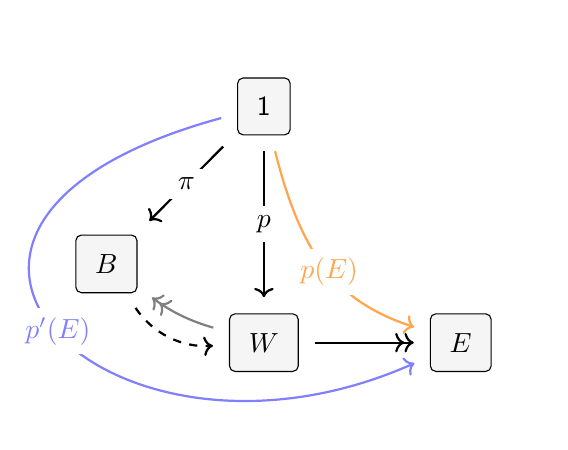
\begin{tikzpicture}[center base]
			\useasboundingbox (-3,-1) rectangle (3.5,4);
			\node[dpadded] (1) at (0,3) {$\sf 1$};
			\node[dpadded] (W) at (0,0) {$W$};
			\node[dpadded] (B) at (-2,1) {$B$};
			\node[dpadded] (E) at (2.5, 0){$E$};
			\coordinate (Q) at (6,0); % to even out controls
			
			\draw[arr] (1) to node[fill=white]{$p$} (W);
			\draw[arr] (1) to node[fill=white]{$\pi$} (B);
			
			\draw[arr, gray, ->>] (W) to[bend left=10] (B);
			\draw[arr, dashed] (B) to[bend right=30] (W);	
			
			\draw[arr, ->>] (W) to (E);
			
			\draw[arr,blue!50] (1) .. controls (-5.5,1.5) and (-2,-2) .. node[fill=white]{$p'(E)$} (E);
			\draw[arr,orange!70] (1) .. controls (0.5,1) and (1,0.5) .. node[fill=white]{$p(E)$} (E);
		\end{tikzpicture}}
		\caption{PDG Belief Updating via Inconsistency}
		\label{fig:belief-update}
	\end{figure}
	
	To understand the update visually in \Cref{fig:belief-update}, imagine the original distribution $p$ from $\sf 1$ to $W$ being replaced by the path $p' := p(W \mid B) \circ \pi$  on the left. The gray arrow on the bottom left is the definition of the random variable, as in \Cref{ex:randomvars}, and the dashed one is its inversion, which can be computed by Bayes' rule.  %that factors through $B$ via the new observation $\pi$.
	To query the resulting distribution on, an arbitrary event $E$, with an indicator variable of the same name. Initially, we got a marginal on $E$ by going through $p$; we now use $p'$. Effectively, the orange path to $E$ has been replaced by the blue one.

	
	To observe $\pi$, we simply view it as a cpd conditioned on $\star$ and add it to our collection. 
	Although it is likely to be inconsistent, resolving this inconsistency in a way that retains $\pi$ is a belief update. 
	Even failure retain $\pi$ entirely may not be a concern: so long as an they continue to observe or remember, an agent endures discomfort until $\pi$ is incorporated. This setting is arguably more natural than a standard one: without spending energy, it is easy to forget or partially reject implications of the observation.	
	Once again, with a PDG, the resolution need not happen immediately. This makes the approach more convincing for cognitively bounded agents, who might have more pressing matters than sorting through beliefs, and who might do them out of order.

	\begin{vfull}
	\section{Algorithms} 
		\label{sec:algorithms}
	\subsection{Belief Propagation}
	
	
	\subsection{Sampling}
	
	One of the nice about directed graphical models is that the model itself is roughly a sampling algorithm. For instance, taking a Bayes Net $\cal B$ and generating samples according to the tables is an efficient way to sample $\Pr_{\mathcal B}$.

	This works because there is only one path, but more generally, for any conditional marginal $Y|X$, we can think of all of the different paths in the PDG different ways an agent with knowledge $\dg M$ can get probabilistic estimates of the conditional distribution $\bbr{\dg M}\MaxEnt(Y | X)$. The next result states that, in a precise sense, these various estimates bound the location of the marginal for this maximum entropy distribution, which suggests an efficient sampling algorithm for $\bbr{\dg M}\MaxEnt(Y | X)$, after learning some weights.
	
	\begin{conj}\label{thm:maxent-hull}
		For any PDG $\dg M = \pdgvars[]$ containing variables $X, Y$, the maximum entropy conditional marginal $\bbr{\dg M}\MaxEnt(y \mid x)$ is a convex mixture of the conditional marginals generated by the paths from $X$ to $Y$.  That is, there exist weights $\{\alpha_i \geq 0\}$ on the paths in $\dg M$ and a bias weight $\alpha_0$ with $\sum_i {\alpha_i} = 1$ and
		\[ \bbr{\dg M}\MaxEnt(Y \mid X) = \alpha_0 \  p^{\text{unif}}_Y \sum_{p \in \bbr{\dg M}_\lambda(X, Y)} \alpha_i (p_1 \circ \ldots \circ p_k) \]
		where $p^{\text{unif}}_Y$ is the uniform distribution on $Y$, and $\bbr{\dg M}_\lambda(X,Y)$ is the set of paths from $X$ to $Y$ generated by composition and Bayes Rule in $\dg M$. 
	\end{conj}

	One natural choice of these $\alpha$'s is the certainty scores for each edge, given by a weighted PDG, but we do not have any further formal results in this direction.
	Note that it is common for humans to make decisions in this way: to estimate whether something is realistic by following multiple chains of reasoning weighting them by strength of argument.
	
%	\begin{conj}
%		The conditional marginal of the maximum entropy distribution $\bbr{M}\MaxEnt(b \mid a)$ is in the convex hull of the compositions of paths $A \to B$. 
%	\end{conj}
	\end{vfull}
}


	\section{Discussion}
        %oli8: entirely rewritten.
%joe7* It will need to be rewritten again, I'm afraid.  We should hint
%at what PDGs are good for: the fact that we can keep track of
%different, possibly conflict sources of information (we should make a
%bigger deal of that in the intro), the fact that we can capture lots
%of distributions (we hinted at that; can we say more?), the fact that
%they are modular (which lets us put together different sources of
%information) and the fact
%that we can model inconsistency and how people recover from
%inconsisency.  This will require us to get into the dynamics of PDGs
%(how people recover from inconsistency) and will require another
%paper, but we should mention it here.  A good discussion will easily
%fill up the 8th page.
%oli9: I agree, this plan sounds excellent. While you do your pass, I will write a draft of this in a separate document. 
%oli10        
\commentout{
	Given more computation, would your beliefs be more consistent? Or would you explore further, forming more extensive networks of them?
	The canonical picture of an idealized agent has always given the first answer, but this may not necessarily be the case.
}
 
 	% Do dogs have more or less consistent beliefs than we do? 
%oli8
	% They may just not have as many concepts.
	% It may be that they are no less consistent, but just have fewer concetpts.

%oli10: deleted the previous text, 
	% We have given the semantics of PDGs, a modeling framework that enables formal reasoning about this kind of mental state, and is strictly more expressive than the class of Bayesian Networks. The scoring semantics for fixed $\beta_L = \gamma = 1$ recovers the factor graph. The distribution given by a PDG, however is not generally this one, but rather one that is as consistent as possible with the supplied cpds.
	% 
	% The material covered in the present paper is only part of the picture. There are two very important generalizations that we plan to cover next. First, by minorly relaxing the definition of a cpd so that it doesn't need to provide a distribution for a special \texttt{null} value, we gain a huge amount of expressive power, allowing for simpler representations of events and partial knowledge.
 	% Second, while we have discussed what happens in the limit as $\gamma \to 0$, emphasizing the quantitative part of the PDG, there is also a rich story to be told about the qualitative half. Together with the modularity provided by the PDG, and the relaxation to strict PDGs, PDGs are able to function as causal models.
%oli10: new text.
%joe9*: rewrote completely.  You have a few lines to say more.  It
%would also be good to squeeze in somewhere something about related
%work (e.g., perhaps dependency networks).
\commentout{
PDGs are a powerful tool for representing local probabilistic information.
	Though represented by a graph, the edges are interpreted
        differently. Each edge alone determines a cpd, making PDGs
        formally analogous to a commutative diagram, instead of a
        flow-chart. A more familiar network can be obtained with the
        use of multi-tailed arrows. 

	PDGs have a parameterized semantics $[[ - ]]_\gamma$, which always generalizes Bayesian Networks, and precisely becomes a factor graph when $\gamma=1$.  This exposes an implicit trade-off between quantitative and qualitative data; the two behave very differently, but are unfortunately fused in a factor graph. Both qualitative and quantitative information can be inconsistent, although the former is less straightforward, this preliminary paper we focus on the quantitative limit.

	Incorporating new variables, data, or restricting to subgraphs
        of a PDG is simple, making it possible to construct one by
        simply throwing together some pre-trained statistical
        models. Moreover, in the quantitative limit, PDGs continue to
        have local meaning, in stark contrast with energy-based models
        such as factor graphs. As a result, PDGs are not only a
        flexible representation, but modular as well. 

	The most dramatic feature of PDGs is their ability to deal with inconsistency. A PDG can track conflicting information from different sources, and its semantics identify when this occurs, rather than quietly sweeping problems under the rug.
	As a result, a user may resolve inconsistency in multiple ways. Inconsistency can be dealt with by updating one or multiple tables, by introducing introducing or splitting variables, or even left unresolved as as one searches for clarification. The pain of inconsistency can be mitigated by expressing a decreased confidence, without altering any data. 
}
%joe9: \end{commenout}
We have introduced PDGs, a powerful tool for representing
probabilistic information. 
%oli11: trying again to integrate some of what I wrote above in
%clearer terms. Note that now the commutative diagram hint comes in
%the syntax section.
%joe10*  NO!!  Do NOT mention commutative diagrams. It's a distraction.
%It's also not true that PDGs are equivalent to BN's when both are
%rooted trees.  You also need to require that there are no parallel
%edges.  I just cut this sentence
%Although PDGs are visually similar to a BNs and equivalent when both
%are rooted trees, a slight change in the way edges are interpreted
%brings them in line with commutative diagrams, 
%and makes them
%oli11: I like this adjective more than you do; you're welcome to find a new one
%dramatically
%%
%more expressive. 
They have a number of advantages of other
graphical representations:
\begin{itemize}
  \item They allow us to capture inconsistency,
including conflict information from multiple sources, and
%oli11
% confidence about pieces of information.
express variable confidence in the information. 
\item 
They are much more
modular 
%oli11: If modularity = flexibility + ability to break into local components with meaning, then I buy this.
% If modularity = flexibility of adding things, it's only true for directed models; factor graphs are modular as hell but difficult to interpret and only have global meaning.
than other representations; 
for example, we can
combine information from two sources by simply taking the union of two
PDGs, and it is easy to add new information 
%oli11 added
%joe10: cut; I don't undrstand what this means
%(edges, including any statistical model you happen to have)
(edges)
%oli11: I want something simpler than "representational capacity" but
%I can't think of what to say instead 
%joe10: I odn't know what ``representational capacity'' means.
%and representational capacity (nodes)
and features (nodes)
%oli11
% regarding nodes and edges
without affecting previously-received information.
%oli11: I like what you have written, but my paragraph above says a
%lot more. I'm trying to merge them to make it clearer. 
%oli11: This local meaning is super important. It was in the equation,
%but I keep not being able to show it directly; I'll try to re-word.  
%joe10: we haven't even defined restrictions, nor have we explained
%this point.  You can't bring it up out of the blue now!  After
%starting to make changs, I just cut this sentence
%oli12: we have now explained the point. I'm inserting a part of this
%again.
%joe11*: we have *not* empahsized the point.  Nowhere do we talk about
%preserving local meanings of cpds, nor explained why this is important.
%In addition to their flexibility (and unlike similarly flexible models
%such factor graphs), PDGs are unique in also preserving the local
%meanings of their cpds.  
%oli13*: This is an important subtlety --- if by "modular" you mean
% flexiblle, then factor graphs are in some sense better than PDGs (you don't
% even need to normalize your factors!), but we have not time or space. 
% I guess I have to drop it..
\commentout{
%In stark contrast to factor graphs,
In contrast to factor graphs,
%joe10: I don't agree
%oli12*: Why not? You can just add a factor anywhere.
%which are equally flexible,
restrictions of PDGs continue to 
%joe10: you keep using words like ``local'' and ``global''; I don't
%know what they mean.  We can't introduce them out of the blue
retain the same local commitment to the meanings of cpds in the
restriction; this is  
As a result, PDGs exhibit both flexibility and locality, making them
uniquely modular. 
}
\item They allow for a clean separation between quantitiatve
  information (the cpds) and more qualitative information contained by
%joe10
%  the graph struture; this is captured by the terms $\Inc$ and $\IDef$
    the graph structure; this is captured by the terms $\Inc$ and $\IDef{}$
  in our scoring function.
\item PDGs have (several) natural semantics;
%oli11 added
%joe10: I don't understand this
  %, each of which paints a global probabilistic picture with
  %  constraints,
%oli12: this was clarified in the semantics introduction now. edited
%and reinstated. 
%joe11: this was *not* clarified in the introduction, and I don't like
%the terminology.  What does it mean to bear on 
%  each of which which bears on global properties of joint distributions,
%  making a PDG more useful than a mere collection of data. 
one of them (under some assumptions) allows us to pick out a unique
distribtuion specified by the PDG.   This, in turn, shows that PDGS 
%joe11: combined
%
%\end{itemize}
%We showed that PDGs
can capture BNs and factor graphs, in the latter case by choosing 
appropriate parameters in the scoring rule. However, they also avoid
%joe10*: let's make sure that we do this
some of the arguably unnatural properties of factor graphs (a point
discussed in more detail in the appendix).
%joe11
\end{itemize}

We have only scratched the surface of what can be done with PDGs here.
%oli11:added
%joe10: this sentence tailed off.  Feel free to add it again
%For simplicitly of presentation, we have only allowed PDGs to express 
%
One issue we hope to foucs on in the future is dynamics.  We believe
that PDGs will prove a particularly useful tool for examining how agents resolve
inconsistency%
%oli11: inefficient use of space
% , moving from an inconsistent state to a consistent state.
.
%oli11: added
%joe10: This is not ``Moreover''.  It's not quite the right story
%Moreover, it seems that the setups to a very large class of standard
%naturally encoded as PDGs, while their standard resolutions (resp.,
%naturally encoded as PDGs; the standard approaches to deal
%with them (resp.,
%variational inference, Bayesian updating) can be regarded as
%reductions of its inconsistency.   
Inconsistency resolution is a pervasive phenomenon.
For example, belief updating can be naturally viewed as an instance of
resolving inconsistency: We now believe that something is true to
which we earlier assigned probabiity less than 1.  Conditioning can be
viewed as a way of resolving that inconsistency (as can other more
general approaches to belief updating, such as Jeffrey's Rule
\cite{Jeffrey68}. 
%joe10: I don't understand how variational inference fits in, but if
%you can write a clear, crisp sentence, we can add it.
%probability less than 
%problems (e.g., variational approximation, belief updating) are
%
This makes representing inconsistent information using a PDG and then
resolving it an topic that can have a potentially high payoff.
We hope to report on this in the future.

	% \subsection{Probabilities Still Encode Well}	
	% In some sense, while we have yet to find a mental state that
	% is not encoded in some probability distribution, the choice
	% of underlying space is extremely important, and we argue
	% that it changes rapidly. Moreover, sometimes one has to make
	% up new internal mental variables, which also changes the
	% underlying space. PDGs offer a way to describe
	% distributions, together with a number of internal parameters
	% one might not be actively aware of. The relevant parameters,
	% can always be internalized \todo{define internalization}
	% until we reach a distribution.  
	% 
	% However, storing knowledge in the form of another graphical model is extremely cumbersome if the set of worlds changes quickly.	
	% 
	% \begin{example}
	% 	\todo{recall coin example, internalize biases, sets of dists, etc.}
	% \end{example}
	% \begin{example}
	% 	\todo{Point to appendix where we discuss factor graph conversions: these internalize the energy}
	% \end{example}
	
	\begin{vfull}
		\subsection{Inconsistency} \label{sec:consistency-ethos}
	
		Believing a logically inconsistent formula can lead you to arbitrarily bad conclusions, having an infeasible set of constraints makes all answers you could give wrong, and having inconsistent preferences can lose you infinite money. We don't want to build inconsistent systems or agents with incoherent views of the world, and so, where possible, we design them so they cannot possibly be broken in this way. Suppose, for example, that we are trying to represent some quantity that must be a point on the unit circle. We could do it with an $x$ and $y$ coordinate, but this could be problematic because $x^2+ y^2$ might not be 1 --- it would be safer and harder to go awry if we parameterize it by an angle $\theta \in [0, 2\pi)$ instead. In the absence of performance benefits (like needing to regularly use the $y$-coordinate and not wanting to compute a sine), why would we take the first approach, introducing a potentially complex data-invariant, when we could avoid it?
		
		This line of thought, though common and defensible, is flawed if we are not perfectly confident in the design of both our system and the ways it can interact with the outside world. Using similar logic, we might ask ourselves: Why ask programmers for type annotations when all instructions are operationally well-defined at run-time?  Why use extra training data if there's already enough there to specify a function? Why estimate a quantity in two ways when they will yield different answers? Why repeat and rephrase your ideas when this could make you contradict yourself? Why write test cases when they could fail and make the project inconsistent? Why conduct an experiment if it could just end up contradicting your current knowledge?
		
		These questions may seem silly, but there is a satisfying information theoretic answer to all of them: redundancy, though costly, is the primary tool that we use to combat the possibility of being wrong. Maintaining data invariants can be expensive but provides diagnostic information; in the example above, settings of $x$ and $y$ that don't lie on the unit circle provide diagnostic information that something has gone wrong.
		In many cases, it is also possible to paper over problems by forcibly re-instating local data invariants: for instance, we could re-normalize any values of $x$ and $y$ (so long as $xy \neq 0$; we can chose an arbitrary point otherwise) at every step. While this would reduce inconsistency, it also hides red flags.
		
		Using a Bayesian Network to represent a probability distribution is like representing a circle with $\theta \in [0, 2\pi)$.
		By construction, the result must be a distribution, and nothing can possibly go wrong so long as we can always decide on exactly one distribution which is sufficient for our purposes.
		%	By construction, the result must be a point on the circle, and nothing can possibly go wrong so long as we're sure that we will always have exactly enough information to determine such a point (for instance, we could never be totally clueless about the point, or just know its $x$ coordinate).
		
		
		The process of mechanistically forcing invariants is homologous to the standard practice for factor graphs: practitioners will often just assume that the density it defines is normalizable, and either forcibly re-normalize or cleverly avoid computing the normalization constant while still assuming that one exists; behavior is usually left unspecified in the unlikely event that it is not defined or zero.
	\end{vfull}
	
	
	
%oli8: removing
	% \section{Conclusions}
	
	% \subsection{A LIST OF PDG BENEFITS}\label{sec:list-of-benefits}
	% \todo{Remove and refactor into appendix}
	% \begin{enumerate}[nosep]
	% 	\item PDGs can represent both over-constrained and under-constrained mental states. 
	% 	\item In particular, they may be inconsistent, which gives agents using PDGs the qualitatively new kind of `epistemic modesty': the possibility of realizing that something is wrong with their beliefs.
	% 	\item Many standard algorithms, including as belief propogation, conditioning, and belief revision, can be regarded as resolution of inconsistency.
	% 	\item PDGs can emulate the functionality of other graphical graphical models.
	% 	\item PDGs are more modular, making it much less invasive to combine, reduce, or partially interpret parts of the model, compared to alternatives.
	% 	\item The modularity enables type-forming rules which can be used to implement deductive inference.
	% 	\item The many standard ways of adding and eliminating variables provides an answer to the question, ``why these possible worlds?''
	% 	\item Compared with a standard constraint satisfaction problem, individual components have of have limited impact on the semantics.
	% 	\item The class of free energies defined by PDGs is strictly more expressive than those given by alternative graphical models.
	% \end{enumerate} % trade-off: harder to analyze.
	
	
	\section*{Broader Impact}
	% Authors are required to include a statement of the broader impact of their work, including its ethical
	% aspects and future societal consequences. Authors should discuss both positive and negative outcomes,
	% if any. For instance, authors should discuss a) who may benefit from this research, b) who may be
	% put at disadvantage from this research, c) what are the consequences of failure of the system, and d)
	% whether the task/method leverages biases in the data. If authors believe this is not applicable to them,
	% authors can simply state this
%joe10*: rewrote
Because PDGs are a recent theoretical development, there is a lot of
guesswork in evaluating the impact. Here are two views of
%joe1
%opposit polarities.
opposite polarity.

\subsection{Positive Impacts}
One can imagine many applications of enabling simple and coherent
aggregation of (possibly inconsistent) information. In particular we
can imagine using PDGs to build and interpret a communal and global
database of statistical models, in a way that may not only enable more
accurate predictions, but also highlights conflicts between
information.

%joe1: what does fairness have to do with any of the above or below?
%This could have a critical impact on the state of fairness.
This could have many benefits.
Suppose, for instance, that two researchers train models, but use
datasets with
different racial makeups. Rather than trying to get an uninterpretable
%joe1
%model to "get it right" the first time, we could simply highlight any
model to ``get it right'' the first time, we could simply highlight any
%joe1
%such clashes and flag them for review---without needing to see
%feedback from the rest of the world.
such clashes and flag them for review.

%joe1: this seems redundant, so I cut it
%It is well-known that the statistically optimal prediction will
%generally not be well-calibrated and fair. 
Rather than trying to
ensure fairness by design which is both tricky and costly,
we envision an alternative: simply use
statistically optimal results, while allowing socail systems to resolve conflicts,
rather than fiddling with loss functions ourselves.
%joe7: \end{commentout}
% \end{notfocus}

\subsection{Negative Impacts}

We can also imagine less rosy outcomes. To the extent that PDGs can
model and reason with inconsistency,
%joe1: I didn't really undesrtand what you wrote below, so I cut it.
%one might worry that PDGs will
%reproduce some of the ``less rational'' human behavior. Because PDGs
%make it so easy to add information without computation, one can
%imagine a naive implementation being particularly vulnerable to
%attacks where it is fed more data than it can reasonably process. As
if
we adopt the attitude that a PDG need not wait until it is consistent
%joe1
%for use, it is not hard to see a world where it gives very biased and
%poorly-thought out conclusions---such a PDG might be likened to a
%conspiracy theorist, constantly absorbing too much information to
%process it correctly.
to be used, it is not hard to imagine a world where a PDG gives biased and
poorly-thought out conclusions.
It is clear that PDGs need a great deal more
vetting before they can be used for such important purposes as
aggregating the world's statistical knowledge.

PDGs are powerful statistical models, but are by necessity
semantically more complicated than many existing methods. This will
likely restrict their accessibility. To mitigate this, we commit to
making sure our work is widely accessible to researchers of different
backgrounds.
        
\begin{ack}
	% \section*{Acknowledgments and Disclosure of Funding}
\end{ack}

%	\section*{References}
%	\printbibliography[heading=none]
{
    \small
    \bibliographystyle{alpha}
    % \bibliography{../refs,../uncertainty,../maths,graphical-models}
    \bibliography{allrefs,z,joe}        
}
%\addbibresource{../uncertainty.bib}
%\addbibresource{../maths.bib}
%\addbibresource{graphical-models.bib}

\appendix
%
\def\year{2021}\relax
% File: formatting-instruction.tex

\documentclass[letterpaper]{article} % DO NOT CHANGE THIS
\usepackage[margin=1in]{geometry}
% \usepackage{aaai21} % DO NOT CHANGE THIS
\usepackage{times} % DO NOT CHANGE THIS
\usepackage{helvet} % DO NOT CHANGE THIS
\usepackage{courier} % DO NOT CHANGE THIS
\usepackage[hyphens]{url} % DO NOT CHANGE THIS
\usepackage{graphicx} % DO NOT CHANGE THIS
\urlstyle{rm} % DO NOT CHANGE THIS
\def\UrlFont{\rm} % DO NOT CHANGE THIS
\usepackage{graphicx} % DO NOT CHANGE THIS
\usepackage{natbib} % DO NOT CHANGE THIS OR ADD OPTIONS
\usepackage{caption} % DO NOT CHANGE THIS OR ADD OPTIONS
\frenchspacing % DO NOT CHANGE THIS
\setlength{\pdfpagewidth}{8.5in} % DO NOT CHANGE THIS
\setlength{\pdfpageheight}{11in} % DO NOT CHANGE THIS

\usepackage{tikz}
	\usetikzlibrary{positioning,fit,calc, decorations, arrows, shapes, shapes.geometric}
	\usetikzlibrary{backgrounds}
	\usetikzlibrary{patterns}
	\usetikzlibrary{cd}
	
	\pgfdeclaredecoration{arrows}{draw}{
		\state{draw}[width=\pgfdecoratedinputsegmentlength]{%
			\path [every arrow subpath/.try] \pgfextra{%
				\pgfpathmoveto{\pgfpointdecoratedinputsegmentfirst}%
				\pgfpathlineto{\pgfpointdecoratedinputsegmentlast}%
			};
	}}
	%%%%%%%%%%%%
	\tikzset{AmpRep/.style={ampersand replacement=\&}}
	\tikzset{center base/.style={baseline={([yshift=-.8ex]current bounding box.center)}}}
	\tikzset{paperfig/.style={center base,scale=0.9, every node/.style={transform shape}}}

	\tikzset{is bn/.style={background rectangle/.style={fill=blue!35,opacity=0.3, rounded corners=5},show background rectangle}}
	% Node Stylings
	\tikzset{dpadded/.style={rounded corners=2, inner sep=0.7em, draw, outer sep=0.3em, fill={black!50}, fill opacity=0.08, text opacity=1}}
	\tikzset{dpad0/.style={outer sep=0.05em, inner sep=0.3em, draw=gray!75, rounded corners=4, fill=black!08, fill opacity=1}}
	\tikzset{dpad/.style args={#1}{every matrix/.append style={nodes={dpadded, #1}}}}
	\tikzset{light pad/.style={outer sep=0.2em, inner sep=0.5em, draw=gray!50}}
		
	\tikzset{arr/.style={draw, ->, thick, shorten <=3pt, shorten >=3pt}}
	\tikzset{arr0/.style={draw, ->, thick, shorten <=0pt, shorten >=0pt}}
	\tikzset{arr1/.style={draw, ->, thick, shorten <=1pt, shorten >=1pt}}
	\tikzset{arr2/.style={draw, ->, thick, shorten <=2pt, shorten >=2pt}}
	\tikzset{archain/.style args={#1}{arr, every arrow subpath/.style={draw,arr, #1}, decoration=arrows, decorate}}


	\tikzset{fgnode/.style={dpadded,inner sep=0.6em, circle},
	factor/.style={light pad, fill=black}}	
	
	
	\newcommand\cmergearr[4]{
		\draw[arr,-] (#1) -- (#4) -- (#2);
		\draw[arr, shorten <=0] (#4) -- (#3);
	}
	\newcommand\mergearr[3]{
		\coordinate (center-#1#2#3) at (barycentric cs:#1=1,#2=1,#3=1.2);
		\cmergearr{#1}{#2}{#3}{center-#1#2#3}
	}
	\newcommand\cunmergearr[4]{
		\draw[arr,-, , shorten >=0] (#1) -- (#4);
		\draw[arr, shorten <=0] (#4) -- (#2);
		\draw[arr, shorten <=0] (#4) -- (#3);
	}
	\newcommand\unmergearr[3]{
		\coordinate (center-#1#2#3) at (barycentric cs:#1=1.2,#2=1,#3=1);
		\cunmergearr{#1}{#2}{#3}{center-#1#2#3}
	}

	
	\usetikzlibrary{matrix}
	\tikzset{toprule/.style={%
	        execute at end cell={%
	            \draw [line cap=rect,#1] 
	            (\tikzmatrixname-\the\pgfmatrixcurrentrow-\the\pgfmatrixcurrentcolumn.north west) -- (\tikzmatrixname-\the\pgfmatrixcurrentrow-\the\pgfmatrixcurrentcolumn.north east);%
	        }
	    },
	    bottomrule/.style={%
	        execute at end cell={%
	            \draw [line cap=rect,#1] (\tikzmatrixname-\the\pgfmatrixcurrentrow-\the\pgfmatrixcurrentcolumn.south west) -- (\tikzmatrixname-\the\pgfmatrixcurrentrow-\the\pgfmatrixcurrentcolumn.south east);%
	        }
	    },
	    leftrule/.style={%
	        execute at end cell={%
	            \draw [line cap=rect,#1] (\tikzmatrixname-\the\pgfmatrixcurrentrow-\the\pgfmatrixcurrentcolumn.north west) -- (\tikzmatrixname-\the\pgfmatrixcurrentrow-\the\pgfmatrixcurrentcolumn.south west);%
	        }
	    },
	    rightrule/.style={%
	        execute at end cell={%
	            \draw [line cap=rect,#1] (\tikzmatrixname-\the\pgfmatrixcurrentrow-\the\pgfmatrixcurrentcolumn.north east) -- (\tikzmatrixname-\the\pgfmatrixcurrentrow-\the\pgfmatrixcurrentcolumn.south east);%
	        }
	    },
	    table with head/.style={
		    matrix of nodes,
		    row sep=-\pgflinewidth,
		    column sep=-\pgflinewidth,
		    nodes={rectangle,minimum width=2.5em, outer sep=0pt},
		    row 1/.style={toprule=thick, bottomrule},
  	    }
	}
\newif\ifprecompiledfigs
\precompiledfigsfalse
% \precompiledfigstrue

\newif\ifexternalizefigures\externalizefiguresfalse

\newif\ifappendix\appendixtrue
\newif\ifbody\bodyfalse

\ifexternalizefigures\else
	\usetikzlibrary{external}
	\tikzexternalize[prefix=tikz/]  % activate!
	% \usepackage{etoolbox}
	%  \AtBeginEnvironment{tikzcd}{\tikzexternaldisable} %... except careful of tikzcd...
	%  \AtEndEnvironment{tikzcd}{\tikzexternalenable}
\fi
%END_FOLD


%BEGIN_FOLD: Theorems and Tools

\usepackage{booktabs}       % professional-quality tables
\usepackage{amsfonts}       % blackboard math symbols
\usepackage{nicefrac}       % compact symbols for 1/2, etc.
\usepackage{microtype}      % microtypography
\usepackage{mathtools}		%also loads amsmath
\usepackage{amssymb, bbm}

%oli20: oops, this is vorboten :(
% \usepackage[format=plain,
%             labelfont={sl},
%             textfont={it,small}]{caption}

\usepackage{relsize}
\usepackage{environ} % http://ctan.org/pkg/environ; for capturing body as a parameter for idxmats

\usepackage{color}
%\usepackage{stmaryrd}

\usepackage{amsthm}
\usepackage{thmtools}

\theoremstyle{plain}
\newtheorem{theorem}{Theorem}[section]
\newtheorem{coro}{Corollary}[theorem]
\newtheorem{prop}[theorem]{Proposition}
\newtheorem{lemma}[theorem]{Lemma}
\newtheorem{fact}[theorem]{Fact}
\newtheorem{conj}[theorem]{Conjecture}

\theoremstyle{definition}

% no section numbers for theorems in AAAI style ... 
%joe17: can you reinstate this?
%oli20:done
\declaretheorem[name=Definition,qed=$\square$,numberwithin=section]{defn} %
\declaretheorem[name=Construction,qed=$\square$,sibling=defn]{constr}
\declaretheorem[qed=$\square$]{example}

\theoremstyle{remark}
\newtheorem*{remark}{Remark}

\usepackage{xstring}
\usepackage{enumitem}

\usepackage{environ}
\usepackage{xstring}

% Wow this works I'm brilliant
\def\wrapwith#1[#2;#3]{
	\expandarg\IfSubStr{#1}{,}{
		\expandafter#2{\expandarg\StrBefore{#1}{,}}
		\expandarg\StrBehind{#1}{,}[\tmp]
		\xdef\tmp{\expandafter\unexpanded\expandafter{\tmp}}
		#3
		\wrapwith{\tmp}[#2;{#3}]
	}{ \expandafter#2{#1} }
}
\def\hwrapcells#1[#2]{\wrapwith#1[#2;&]}
\def\vwrapcells#1[#2]{\wrapwith#1[#2;\\]}
\NewEnviron{mymathenv}{$\BODY$}

\newcommand{\smalltext}[1]{\text{\footnotesize#1}}
\newsavebox{\idxmatsavebox}
\def\makeinvisibleidxstyle#1#2{\phantom{\hbox{#1#2}}}
\newenvironment{idxmatphant}[4][\color{gray}\smalltext]{%
	\def\idxstyle{#1}
	\def\colitems{#3}
	\def\rowitems{#2}
	\def\phantitems{#4}
	\begin{lrbox}{\idxmatsavebox}$%$\begin{mymathenv}
	\begin{matrix}  \begin{matrix} \hwrapcells{\colitems}[\idxstyle]  \end{matrix}
		% &\vphantom{\idxstyle\colitems}
		\\[-0.05em]
		\left[
		\begin{matrix}
			\hwrapcells{\phantitems}[\expandafter\makeinvisibleidxstyle\idxstyle]  \\[-1.2em]
	}{
		\end{matrix}\right]		&\hspace{-0.8em}\begin{matrix*}[l] \vwrapcells{\rowitems}[\idxstyle] \end{matrix*}\hspace{0.1em}%
	\end{matrix}%
	$%\end{mymathenv}
	\end{lrbox}%
	\raisebox{0.75em}{\usebox\idxmatsavebox}
%	\vspace{-0.5em}
}

\newenvironment{idxmat}[3][\color{gray}\smalltext]
	{\begingroup\idxmatphant[#1]{#2}{#3}{#3}}
	{\endidxmatphant\endgroup}

\newenvironment{sqidxmat}[2][\color{gray}\smalltext]
	{\begingroup\idxmat[#1]{#2}{#2}}
	{\endidxmat\endgroup}


%%%%%%%%%%%%
% better alignment for cases
\makeatletter
\renewenvironment{cases}[1][l]{\matrix@check\cases\env@cases{#1}}{\endarray\right.}
\def\env@cases#1{%
	\let\@ifnextchar\new@ifnextchar
	\left\lbrace\def\arraystretch{1.2}%
	\array{@{}#1@{\quad}l@{}}}
\makeatother

\newcommand\numberthis{\addtocounter{equation}{1}\tag{\theequation}}

%oli20: apparently this is not allowed in AAAI style.
%oli21: but it helps me edit so I'm reenabling it until later
%oli25:
% \usepackage{xr}
% \usepackage{xr-hyper}
\usepackage{zref-xr}
% \usepackage{hyperref}
\zxrsetup{toltxlabel=true, tozreflabel=false}
\zexternaldocument*{pdg}
%oli24: the time has come... goodbye links and colors :(
% \usepackage{hyperref}
% \definecolor{deepgreen}{rgb}{0,0.5,0}
% \hypersetup{colorlinks=true, linkcolor=blue!50!black, urlcolor=magenta, citecolor=deepgreen}

\usepackage[noabbrev,nameinlink,capitalize]{cleveref}
\crefname{example}{Example}{Examples}
\crefname{defn}{Definition}{Definitions}
\crefname{prop}{Proposition}{Propositions}
\crefname{constr}{Construction}{Constructions}
\crefname{conj}{Conjecture}{Conjectures}
\crefname{fact}{Fact}{Facts}
%\crefname{section}{\S\!}{\S\!}


\usepackage{float}
% \usepackage{subcaption}
\newcounter{subfigure}
	% \captionsetup[subfigure]{subrefformat=simple,labelformat=simple}
	\renewcommand\thesubfigure{\thefigure(\alph{subfigure})}
    
\newenvironment{old}[1]{\par\noindent{\bf \Cref{#1}.} \em \noindent}{\par\medskip}

%% Version of recall that pulls the savebox:
% \usepackage{xpatch}
% \makeatletter
% \xpatchcmd{\thmt@restatable}% Edit \thmt@restatable
%    {\csname #2\@xa\endcsname\ifx\@nx#1\@nx\else[{#1}]\fi}% Replace this code
%    % {\ifthmt@thisistheone\csname #2\@xa\endcsname\typeout{oiii[#1;#2\@xa;#3;\csname thmt@stored@#3\endcsname]}\ifx\@nx#1\@nx\else[#1]\fi\else\csname #2\@xa\endcsname\fi}% with this code
%    {\ifthmt@thisistheone\csname #2\@xa\endcsname\ifx\@nx#1\@nx\else[{#1}]\fi
%    \else\fi}
%    {\typeout{oii Success1?}}{\typeout{oiii failure1?}} % execute code for success/failure instances
% \xpatchcmd{\thmt@restatable}% Edit \thmt@restatable
%    {\csname end#2\endcsname}
%    {\ifthmt@thisistheone\csname end#2\endcsname\else\fi}
%    {\typeout{oii Success2?}}{\typeout{oiii failure2?}}
% \newcommand{\recall}[1]{\medskip\par\noindent{\bf \expandarg\Cref{thmt@@#1}.} \begingroup\em \noindent
%    \expandafter\csname#1\endcsname* \endgroup\par\smallskip}
% \makeatother

\newcommand{\restate}[2]
	{\medskip\par\noindent{\bf \expandarg\Cref{thmt@@#1}.}%
 	\noindent\begingroup\em #2 \endgroup\par\smallskip}


%oli16: The extra space was because there was extra space in the paragraph, not
%because this length was too big. By breaking arrays, everything will be better.
\allowdisplaybreaks

\newcommand{\begthm}[3][]{\begin{#2}[{name=#1},restate=#3,label=#3]}

%TODO
\newcommand{\createversion}[2][{gray}{0.75}]{
	\definecolor{v#2color}#1\relax
    \expandafter\xdef\csname v#2on\endcsname{%
		% \xdef\gamma{\tau}%
		% \expandafter\renewcommand\csname v#2\endcsname{ONN}%
		% \expandafter\xdef{\csname v#2on\endcsname}##{{\color{v##2color} #1}}
	}
	\expandafter\xdef\csname v#2off\endcsname{
	% 	\expandafter\newcommand\csname v #2\endcsname[1]{{\color{v ##2 color} #1}}
	}
}
\createversion{test}
% \vteston
%END_FOLD

%BEGIN_FOLD   %%%% Version knobs %%%%%. 
%oli20: your commenting system is better than the one based on comment package, 
% which is way more problematic than I thought.
% I'm killing it and refactoring all comments to be like yours. I'm not annotating
% everything I'm doing here but the result will be way clearer and less problematic.

\definecolor{vfullcolor}{gray}{0.7}
\newcommand\vfull[1]{{\color{vfullcolor} #1}}
\renewcommand\vfull[1]{} % disable vfull

\definecolor{vleftoverscolor}{gray}{0.85}
\newcommand{\vleftovers}[1]{{\color{vleftoverscolor} #1}} 
\renewcommand{\vleftovers}[1]{} %disable vleftovers

\definecolor{notationcolor}{rgb}{0.9,0.9,.9} 
\newcommand{\notation}[1]{{\color{notationcolor} #1}}
\renewcommand{\notation}[1]{\ignorespaces} % disable notation

\definecolor{contentiouscolor}{rgb}{0.7,0.3,.1} 
\newcommand{\commentout}[1]{\ignorespaces} 

% \newcommand{\contentious}[1]{
% 	\noindent\colorbox{red!10!white}{\parbox{\linewidth-3pt}{\color{red!10!black}#1}}}
% \newcommand{\valpha}[1]{%
% 	% \colorbox{red!10!white}
% 	{\color{red!10!black}{#1}}%
% }
% \newcommand{\valpha}[1]{{\color{red!80!black}#1}}
\newcommand{\valpha}[1]{#1}

%END_FOLD


%BEGIN_FOLD definitions
%BEGIN_FOLD %%%%%   general shorthand I use   %%%%%%%%%%%%%%%%%

%\usepackage{stmaryrd}
%\DeclarePairedDelimiter{\ccbr}{\lBrace}{\rBrace}
%\DeclarePairedDelimiter{\bbr}{\llbracket}{\rrbracket}
%\DeclarePairedDelimiter{\ppr}{\llparenthesis}{\rrparenthesis}

\DeclarePairedDelimiterX{\bbr}[1]{[}{]}{\mspace{-3.5mu}\delimsize[#1\delimsize]\mspace{-3.5mu}}
\DeclarePairedDelimiter{\norm}{\lVert}{\rVert}

\let\Horig\H
\let\H\relax
\DeclareMathOperator{\H}{\mathrm{H}} % Entropy
\DeclareMathOperator{\I}{\mathrm{I}} % Information
\DeclareMathOperator*{\Ex}{\mathbb{E}} % Expectation
\DeclareMathOperator*{\argmin}{arg\;min}
\newcommand{\CI}{\mathrel{\perp\mspace{-10mu}\perp}} % Conditional Independence
\newcommand\mat[1]{\mathbf{#1}}
\DeclarePairedDelimiterX{\infdivx}[2]{(}{)}{%
	#1\;\delimsize\|\;#2%
}
\newcommand{\thickD}{I\mkern-8muD}
\newcommand{\kldiv}{\thickD\infdivx}


\newcommand{\todo}[1]{{\color{red}\ \!\Large\smash{\textbf{[}}{\normalsize\textsc{todo:} #1}\ \!\smash{\textbf{]}}}}
\newcommand{\note}[1]{{\color{blue}\ \!\Large\smash{\textbf{[}}{\normalsize\textsc{note:} #1}\ \!\smash{\textbf{]}}}}



% SPACES
\newcommand\Set{\mathbb{S}\mathrm{et}}
\newcommand\FinSet{\mathbb{F}\mathrm{in}\mathrm{S}\mathrm{et}}
\newcommand\Meas{\mathbb{M}\mathrm{eas}}
\newcommand\two{\mathbbm 2}

%END_FOLD

%BEGIN_FOLD %%%%%    PDG-specific macros     %%%%%%%%%%%%%%%%
\DeclarePairedDelimiterXPP{\SD}[1]{}{[}{]}{_{\text{sd}}}{\mspace{-3.5mu}\delimsize[#1\delimsize]\mspace{-3.5mu}}
		
%\usepackage{stmaryrd}
%\newcommand{\none}{\varobslash}
\newcommand{\none}{\bullet}

\def\sheq{\!=\!}
\DeclareMathOperator\dcap{\mathop{\dot\cap}}
\newcommand{\tto}{\rightarrow\mathrel{\mspace{-15mu}}\rightarrow}

\newcommand{\bp}[1][L]{\mat{p}_{\!_{#1}\!}}
\newcommand{\V}{\mathcal V}
\newcommand{\N}{\mathcal N}
\newcommand{\Ed}{\mathcal E}
\newcommand{\pdgvars}[1][]{(\N#1, \Ed#1, \V#1, \mat p#1, \beta#1)}


\DeclareMathAlphabet{\mathdcal}{U}{dutchcal}{m}{n}
\DeclareMathAlphabet{\mathbdcal}{U}{dutchcal}{b}{n}
%joe1:out of curiousity, why not use \mathcal?  That's what you use
%for BNs.  Why do PDG use a different font?
\newcommand{\dg}[1]{\mathbdcal{#1}}
\newcommand{\var}[1]{\mathsf{#1}}
\newcommand\Pa{\mathbf{Pa}}

%oli20: better spacing
% \newcommand{\IDef}[1]{\mathit{IDef}_{#1}}
\newcommand{\IDef}[1]{\mathit{IDef}_{\!#1}}

\newcommand\Inc{\mathit{Inc}}
\newcommand{\PDGof}[1]{{\dg M}_{#1}}
%oli22: a macro for unweighted PDGs
\newcommand{\UPDGof}[1]{{\dg N}_{#1}}
\newcommand{\WFGof}[1]{\Psi_{{#1}}}
%oli22: and for unweighted ones
\newcommand{\FGof}[1]{\Phi_{{#1}}}
%oli22: want to refer to the variable graph
\newcommand{\Gr}{\mathcal G}
%oli22: Gibbs Free Energy conflicts with \mathcal G. Now it lives in 
% this macro.
\newcommand\GFE{\mathit{G\mkern-4mu F\mkern-4.5mu E}}
%oli22: Right now we're using (\N, \V) to refer to variables of a
% PDG. I think it's important to keep both \N and \V but am happy to change
% the way we combine them. Factored into a macro so it's easier to change.
\newcommand{\varsNV}[1][\N,\V]{(#1)}


% \makeatletter %Arguments: L, X, Y, \scriptscriptstyle, -1pt (for raisebox)
% \newcommand{\ed@helper}[5]{#2\!%
%   \overset{\smash{\mskip-5mu\raisebox{-1pt}{$\scriptscriptstyle
%         #1$}}}{\rightarrow}\! #3} 
% \makeatother

%oli22: the edge notation is now uniform. Choose between the following
% Default: display as "X -L-> Y" (leave uncommented).
\newcommand{\ed}[3]{#2\!%
  \overset{\smash{\mskip-5mu\raisebox{-1pt}{$\scriptscriptstyle
        #1$}}}{\rightarrow}\! #3} 
% Option: uncomment to display as  "L = (X,Y,\ell)" instead.
% \renewcommand{\ed}[3]{#2 = (#1,#3,\ell)} 
\newcommand{\alle}[1][L]{_{ \ed {#1}XY}}


\begin{document}
\appendix
\onecolumn
%
\def\year{2021}\relax
% File: formatting-instruction.tex

\documentclass[letterpaper]{article} % DO NOT CHANGE THIS
\usepackage[margin=1in]{geometry}
% \usepackage{aaai21} % DO NOT CHANGE THIS
\usepackage{times} % DO NOT CHANGE THIS
\usepackage{helvet} % DO NOT CHANGE THIS
\usepackage{courier} % DO NOT CHANGE THIS
\usepackage[hyphens]{url} % DO NOT CHANGE THIS
\usepackage{graphicx} % DO NOT CHANGE THIS
\urlstyle{rm} % DO NOT CHANGE THIS
\def\UrlFont{\rm} % DO NOT CHANGE THIS
\usepackage{graphicx} % DO NOT CHANGE THIS
\usepackage{natbib} % DO NOT CHANGE THIS OR ADD OPTIONS
\usepackage{caption} % DO NOT CHANGE THIS OR ADD OPTIONS
\frenchspacing % DO NOT CHANGE THIS
\setlength{\pdfpagewidth}{8.5in} % DO NOT CHANGE THIS
\setlength{\pdfpageheight}{11in} % DO NOT CHANGE THIS

\usepackage{tikz}
	\usetikzlibrary{positioning,fit,calc, decorations, arrows, shapes, shapes.geometric}
	\usetikzlibrary{backgrounds}
	\usetikzlibrary{patterns}
	\usetikzlibrary{cd}
	
	\pgfdeclaredecoration{arrows}{draw}{
		\state{draw}[width=\pgfdecoratedinputsegmentlength]{%
			\path [every arrow subpath/.try] \pgfextra{%
				\pgfpathmoveto{\pgfpointdecoratedinputsegmentfirst}%
				\pgfpathlineto{\pgfpointdecoratedinputsegmentlast}%
			};
	}}
	%%%%%%%%%%%%
	\tikzset{AmpRep/.style={ampersand replacement=\&}}
	\tikzset{center base/.style={baseline={([yshift=-.8ex]current bounding box.center)}}}
	\tikzset{paperfig/.style={center base,scale=0.9, every node/.style={transform shape}}}

	\tikzset{is bn/.style={background rectangle/.style={fill=blue!35,opacity=0.3, rounded corners=5},show background rectangle}}
	% Node Stylings
	\tikzset{dpadded/.style={rounded corners=2, inner sep=0.7em, draw, outer sep=0.3em, fill={black!50}, fill opacity=0.08, text opacity=1}}
	\tikzset{dpad0/.style={outer sep=0.05em, inner sep=0.3em, draw=gray!75, rounded corners=4, fill=black!08, fill opacity=1}}
	\tikzset{dpad/.style args={#1}{every matrix/.append style={nodes={dpadded, #1}}}}
	\tikzset{light pad/.style={outer sep=0.2em, inner sep=0.5em, draw=gray!50}}
		
	\tikzset{arr/.style={draw, ->, thick, shorten <=3pt, shorten >=3pt}}
	\tikzset{arr0/.style={draw, ->, thick, shorten <=0pt, shorten >=0pt}}
	\tikzset{arr1/.style={draw, ->, thick, shorten <=1pt, shorten >=1pt}}
	\tikzset{arr2/.style={draw, ->, thick, shorten <=2pt, shorten >=2pt}}
	\tikzset{archain/.style args={#1}{arr, every arrow subpath/.style={draw,arr, #1}, decoration=arrows, decorate}}


	\tikzset{fgnode/.style={dpadded,inner sep=0.6em, circle},
	factor/.style={light pad, fill=black}}	
	
	
	\newcommand\cmergearr[4]{
		\draw[arr,-] (#1) -- (#4) -- (#2);
		\draw[arr, shorten <=0] (#4) -- (#3);
	}
	\newcommand\mergearr[3]{
		\coordinate (center-#1#2#3) at (barycentric cs:#1=1,#2=1,#3=1.2);
		\cmergearr{#1}{#2}{#3}{center-#1#2#3}
	}
	\newcommand\cunmergearr[4]{
		\draw[arr,-, , shorten >=0] (#1) -- (#4);
		\draw[arr, shorten <=0] (#4) -- (#2);
		\draw[arr, shorten <=0] (#4) -- (#3);
	}
	\newcommand\unmergearr[3]{
		\coordinate (center-#1#2#3) at (barycentric cs:#1=1.2,#2=1,#3=1);
		\cunmergearr{#1}{#2}{#3}{center-#1#2#3}
	}

	
	\usetikzlibrary{matrix}
	\tikzset{toprule/.style={%
	        execute at end cell={%
	            \draw [line cap=rect,#1] 
	            (\tikzmatrixname-\the\pgfmatrixcurrentrow-\the\pgfmatrixcurrentcolumn.north west) -- (\tikzmatrixname-\the\pgfmatrixcurrentrow-\the\pgfmatrixcurrentcolumn.north east);%
	        }
	    },
	    bottomrule/.style={%
	        execute at end cell={%
	            \draw [line cap=rect,#1] (\tikzmatrixname-\the\pgfmatrixcurrentrow-\the\pgfmatrixcurrentcolumn.south west) -- (\tikzmatrixname-\the\pgfmatrixcurrentrow-\the\pgfmatrixcurrentcolumn.south east);%
	        }
	    },
	    leftrule/.style={%
	        execute at end cell={%
	            \draw [line cap=rect,#1] (\tikzmatrixname-\the\pgfmatrixcurrentrow-\the\pgfmatrixcurrentcolumn.north west) -- (\tikzmatrixname-\the\pgfmatrixcurrentrow-\the\pgfmatrixcurrentcolumn.south west);%
	        }
	    },
	    rightrule/.style={%
	        execute at end cell={%
	            \draw [line cap=rect,#1] (\tikzmatrixname-\the\pgfmatrixcurrentrow-\the\pgfmatrixcurrentcolumn.north east) -- (\tikzmatrixname-\the\pgfmatrixcurrentrow-\the\pgfmatrixcurrentcolumn.south east);%
	        }
	    },
	    table with head/.style={
		    matrix of nodes,
		    row sep=-\pgflinewidth,
		    column sep=-\pgflinewidth,
		    nodes={rectangle,minimum width=2.5em, outer sep=0pt},
		    row 1/.style={toprule=thick, bottomrule},
  	    }
	}
\newif\ifprecompiledfigs
\precompiledfigsfalse
% \precompiledfigstrue

\newif\ifexternalizefigures\externalizefiguresfalse

\newif\ifappendix\appendixtrue
\newif\ifbody\bodyfalse

\ifexternalizefigures\else
	\usetikzlibrary{external}
	\tikzexternalize[prefix=tikz/]  % activate!
	% \usepackage{etoolbox}
	%  \AtBeginEnvironment{tikzcd}{\tikzexternaldisable} %... except careful of tikzcd...
	%  \AtEndEnvironment{tikzcd}{\tikzexternalenable}
\fi
%END_FOLD


%BEGIN_FOLD: Theorems and Tools

\usepackage{booktabs}       % professional-quality tables
\usepackage{amsfonts}       % blackboard math symbols
\usepackage{nicefrac}       % compact symbols for 1/2, etc.
\usepackage{microtype}      % microtypography
\usepackage{mathtools}		%also loads amsmath
\usepackage{amssymb, bbm}

%oli20: oops, this is vorboten :(
% \usepackage[format=plain,
%             labelfont={sl},
%             textfont={it,small}]{caption}

\usepackage{relsize}
\usepackage{environ} % http://ctan.org/pkg/environ; for capturing body as a parameter for idxmats

\usepackage{color}
%\usepackage{stmaryrd}

\usepackage{amsthm}
\usepackage{thmtools}

\theoremstyle{plain}
\newtheorem{theorem}{Theorem}[section]
\newtheorem{coro}{Corollary}[theorem]
\newtheorem{prop}[theorem]{Proposition}
\newtheorem{lemma}[theorem]{Lemma}
\newtheorem{fact}[theorem]{Fact}
\newtheorem{conj}[theorem]{Conjecture}

\theoremstyle{definition}

% no section numbers for theorems in AAAI style ... 
%joe17: can you reinstate this?
%oli20:done
\declaretheorem[name=Definition,qed=$\square$,numberwithin=section]{defn} %
\declaretheorem[name=Construction,qed=$\square$,sibling=defn]{constr}
\declaretheorem[qed=$\square$]{example}

\theoremstyle{remark}
\newtheorem*{remark}{Remark}

\usepackage{xstring}
\usepackage{enumitem}

\usepackage{environ}
\usepackage{xstring}

% Wow this works I'm brilliant
\def\wrapwith#1[#2;#3]{
	\expandarg\IfSubStr{#1}{,}{
		\expandafter#2{\expandarg\StrBefore{#1}{,}}
		\expandarg\StrBehind{#1}{,}[\tmp]
		\xdef\tmp{\expandafter\unexpanded\expandafter{\tmp}}
		#3
		\wrapwith{\tmp}[#2;{#3}]
	}{ \expandafter#2{#1} }
}
\def\hwrapcells#1[#2]{\wrapwith#1[#2;&]}
\def\vwrapcells#1[#2]{\wrapwith#1[#2;\\]}
\NewEnviron{mymathenv}{$\BODY$}

\newcommand{\smalltext}[1]{\text{\footnotesize#1}}
\newsavebox{\idxmatsavebox}
\def\makeinvisibleidxstyle#1#2{\phantom{\hbox{#1#2}}}
\newenvironment{idxmatphant}[4][\color{gray}\smalltext]{%
	\def\idxstyle{#1}
	\def\colitems{#3}
	\def\rowitems{#2}
	\def\phantitems{#4}
	\begin{lrbox}{\idxmatsavebox}$%$\begin{mymathenv}
	\begin{matrix}  \begin{matrix} \hwrapcells{\colitems}[\idxstyle]  \end{matrix}
		% &\vphantom{\idxstyle\colitems}
		\\[-0.05em]
		\left[
		\begin{matrix}
			\hwrapcells{\phantitems}[\expandafter\makeinvisibleidxstyle\idxstyle]  \\[-1.2em]
	}{
		\end{matrix}\right]		&\hspace{-0.8em}\begin{matrix*}[l] \vwrapcells{\rowitems}[\idxstyle] \end{matrix*}\hspace{0.1em}%
	\end{matrix}%
	$%\end{mymathenv}
	\end{lrbox}%
	\raisebox{0.75em}{\usebox\idxmatsavebox}
%	\vspace{-0.5em}
}

\newenvironment{idxmat}[3][\color{gray}\smalltext]
	{\begingroup\idxmatphant[#1]{#2}{#3}{#3}}
	{\endidxmatphant\endgroup}

\newenvironment{sqidxmat}[2][\color{gray}\smalltext]
	{\begingroup\idxmat[#1]{#2}{#2}}
	{\endidxmat\endgroup}


%%%%%%%%%%%%
% better alignment for cases
\makeatletter
\renewenvironment{cases}[1][l]{\matrix@check\cases\env@cases{#1}}{\endarray\right.}
\def\env@cases#1{%
	\let\@ifnextchar\new@ifnextchar
	\left\lbrace\def\arraystretch{1.2}%
	\array{@{}#1@{\quad}l@{}}}
\makeatother

\newcommand\numberthis{\addtocounter{equation}{1}\tag{\theequation}}

%oli20: apparently this is not allowed in AAAI style.
%oli21: but it helps me edit so I'm reenabling it until later
%oli25:
% \usepackage{xr}
% \usepackage{xr-hyper}
\usepackage{zref-xr}
% \usepackage{hyperref}
\zxrsetup{toltxlabel=true, tozreflabel=false}
\zexternaldocument*{pdg}
%oli24: the time has come... goodbye links and colors :(
% \usepackage{hyperref}
% \definecolor{deepgreen}{rgb}{0,0.5,0}
% \hypersetup{colorlinks=true, linkcolor=blue!50!black, urlcolor=magenta, citecolor=deepgreen}

\usepackage[noabbrev,nameinlink,capitalize]{cleveref}
\crefname{example}{Example}{Examples}
\crefname{defn}{Definition}{Definitions}
\crefname{prop}{Proposition}{Propositions}
\crefname{constr}{Construction}{Constructions}
\crefname{conj}{Conjecture}{Conjectures}
\crefname{fact}{Fact}{Facts}
%\crefname{section}{\S\!}{\S\!}


\usepackage{float}
% \usepackage{subcaption}
\newcounter{subfigure}
	% \captionsetup[subfigure]{subrefformat=simple,labelformat=simple}
	\renewcommand\thesubfigure{\thefigure(\alph{subfigure})}
    
\newenvironment{old}[1]{\par\noindent{\bf \Cref{#1}.} \em \noindent}{\par\medskip}

%% Version of recall that pulls the savebox:
% \usepackage{xpatch}
% \makeatletter
% \xpatchcmd{\thmt@restatable}% Edit \thmt@restatable
%    {\csname #2\@xa\endcsname\ifx\@nx#1\@nx\else[{#1}]\fi}% Replace this code
%    % {\ifthmt@thisistheone\csname #2\@xa\endcsname\typeout{oiii[#1;#2\@xa;#3;\csname thmt@stored@#3\endcsname]}\ifx\@nx#1\@nx\else[#1]\fi\else\csname #2\@xa\endcsname\fi}% with this code
%    {\ifthmt@thisistheone\csname #2\@xa\endcsname\ifx\@nx#1\@nx\else[{#1}]\fi
%    \else\fi}
%    {\typeout{oii Success1?}}{\typeout{oiii failure1?}} % execute code for success/failure instances
% \xpatchcmd{\thmt@restatable}% Edit \thmt@restatable
%    {\csname end#2\endcsname}
%    {\ifthmt@thisistheone\csname end#2\endcsname\else\fi}
%    {\typeout{oii Success2?}}{\typeout{oiii failure2?}}
% \newcommand{\recall}[1]{\medskip\par\noindent{\bf \expandarg\Cref{thmt@@#1}.} \begingroup\em \noindent
%    \expandafter\csname#1\endcsname* \endgroup\par\smallskip}
% \makeatother

\newcommand{\restate}[2]
	{\medskip\par\noindent{\bf \expandarg\Cref{thmt@@#1}.}%
 	\noindent\begingroup\em #2 \endgroup\par\smallskip}


%oli16: The extra space was because there was extra space in the paragraph, not
%because this length was too big. By breaking arrays, everything will be better.
\allowdisplaybreaks

\newcommand{\begthm}[3][]{\begin{#2}[{name=#1},restate=#3,label=#3]}

%TODO
\newcommand{\createversion}[2][{gray}{0.75}]{
	\definecolor{v#2color}#1\relax
    \expandafter\xdef\csname v#2on\endcsname{%
		% \xdef\gamma{\tau}%
		% \expandafter\renewcommand\csname v#2\endcsname{ONN}%
		% \expandafter\xdef{\csname v#2on\endcsname}##{{\color{v##2color} #1}}
	}
	\expandafter\xdef\csname v#2off\endcsname{
	% 	\expandafter\newcommand\csname v #2\endcsname[1]{{\color{v ##2 color} #1}}
	}
}
\createversion{test}
% \vteston
%END_FOLD

%BEGIN_FOLD   %%%% Version knobs %%%%%. 
%oli20: your commenting system is better than the one based on comment package, 
% which is way more problematic than I thought.
% I'm killing it and refactoring all comments to be like yours. I'm not annotating
% everything I'm doing here but the result will be way clearer and less problematic.

\definecolor{vfullcolor}{gray}{0.7}
\newcommand\vfull[1]{{\color{vfullcolor} #1}}
\renewcommand\vfull[1]{} % disable vfull

\definecolor{vleftoverscolor}{gray}{0.85}
\newcommand{\vleftovers}[1]{{\color{vleftoverscolor} #1}} 
\renewcommand{\vleftovers}[1]{} %disable vleftovers

\definecolor{notationcolor}{rgb}{0.9,0.9,.9} 
\newcommand{\notation}[1]{{\color{notationcolor} #1}}
\renewcommand{\notation}[1]{\ignorespaces} % disable notation

\definecolor{contentiouscolor}{rgb}{0.7,0.3,.1} 
\newcommand{\commentout}[1]{\ignorespaces} 

% \newcommand{\contentious}[1]{
% 	\noindent\colorbox{red!10!white}{\parbox{\linewidth-3pt}{\color{red!10!black}#1}}}
% \newcommand{\valpha}[1]{%
% 	% \colorbox{red!10!white}
% 	{\color{red!10!black}{#1}}%
% }
% \newcommand{\valpha}[1]{{\color{red!80!black}#1}}
\newcommand{\valpha}[1]{#1}

%END_FOLD


%BEGIN_FOLD definitions
%BEGIN_FOLD %%%%%   general shorthand I use   %%%%%%%%%%%%%%%%%

%\usepackage{stmaryrd}
%\DeclarePairedDelimiter{\ccbr}{\lBrace}{\rBrace}
%\DeclarePairedDelimiter{\bbr}{\llbracket}{\rrbracket}
%\DeclarePairedDelimiter{\ppr}{\llparenthesis}{\rrparenthesis}

\DeclarePairedDelimiterX{\bbr}[1]{[}{]}{\mspace{-3.5mu}\delimsize[#1\delimsize]\mspace{-3.5mu}}
\DeclarePairedDelimiter{\norm}{\lVert}{\rVert}

\let\Horig\H
\let\H\relax
\DeclareMathOperator{\H}{\mathrm{H}} % Entropy
\DeclareMathOperator{\I}{\mathrm{I}} % Information
\DeclareMathOperator*{\Ex}{\mathbb{E}} % Expectation
\DeclareMathOperator*{\argmin}{arg\;min}
\newcommand{\CI}{\mathrel{\perp\mspace{-10mu}\perp}} % Conditional Independence
\newcommand\mat[1]{\mathbf{#1}}
\DeclarePairedDelimiterX{\infdivx}[2]{(}{)}{%
	#1\;\delimsize\|\;#2%
}
\newcommand{\thickD}{I\mkern-8muD}
\newcommand{\kldiv}{\thickD\infdivx}


\newcommand{\todo}[1]{{\color{red}\ \!\Large\smash{\textbf{[}}{\normalsize\textsc{todo:} #1}\ \!\smash{\textbf{]}}}}
\newcommand{\note}[1]{{\color{blue}\ \!\Large\smash{\textbf{[}}{\normalsize\textsc{note:} #1}\ \!\smash{\textbf{]}}}}



% SPACES
\newcommand\Set{\mathbb{S}\mathrm{et}}
\newcommand\FinSet{\mathbb{F}\mathrm{in}\mathrm{S}\mathrm{et}}
\newcommand\Meas{\mathbb{M}\mathrm{eas}}
\newcommand\two{\mathbbm 2}

%END_FOLD

%BEGIN_FOLD %%%%%    PDG-specific macros     %%%%%%%%%%%%%%%%
\DeclarePairedDelimiterXPP{\SD}[1]{}{[}{]}{_{\text{sd}}}{\mspace{-3.5mu}\delimsize[#1\delimsize]\mspace{-3.5mu}}
		
%\usepackage{stmaryrd}
%\newcommand{\none}{\varobslash}
\newcommand{\none}{\bullet}

\def\sheq{\!=\!}
\DeclareMathOperator\dcap{\mathop{\dot\cap}}
\newcommand{\tto}{\rightarrow\mathrel{\mspace{-15mu}}\rightarrow}

\newcommand{\bp}[1][L]{\mat{p}_{\!_{#1}\!}}
\newcommand{\V}{\mathcal V}
\newcommand{\N}{\mathcal N}
\newcommand{\Ed}{\mathcal E}
\newcommand{\pdgvars}[1][]{(\N#1, \Ed#1, \V#1, \mat p#1, \beta#1)}


\DeclareMathAlphabet{\mathdcal}{U}{dutchcal}{m}{n}
\DeclareMathAlphabet{\mathbdcal}{U}{dutchcal}{b}{n}
%joe1:out of curiousity, why not use \mathcal?  That's what you use
%for BNs.  Why do PDG use a different font?
\newcommand{\dg}[1]{\mathbdcal{#1}}
\newcommand{\var}[1]{\mathsf{#1}}
\newcommand\Pa{\mathbf{Pa}}

%oli20: better spacing
% \newcommand{\IDef}[1]{\mathit{IDef}_{#1}}
\newcommand{\IDef}[1]{\mathit{IDef}_{\!#1}}

\newcommand\Inc{\mathit{Inc}}
\newcommand{\PDGof}[1]{{\dg M}_{#1}}
%oli22: a macro for unweighted PDGs
\newcommand{\UPDGof}[1]{{\dg N}_{#1}}
\newcommand{\WFGof}[1]{\Psi_{{#1}}}
%oli22: and for unweighted ones
\newcommand{\FGof}[1]{\Phi_{{#1}}}
%oli22: want to refer to the variable graph
\newcommand{\Gr}{\mathcal G}
%oli22: Gibbs Free Energy conflicts with \mathcal G. Now it lives in 
% this macro.
\newcommand\GFE{\mathit{G\mkern-4mu F\mkern-4.5mu E}}
%oli22: Right now we're using (\N, \V) to refer to variables of a
% PDG. I think it's important to keep both \N and \V but am happy to change
% the way we combine them. Factored into a macro so it's easier to change.
\newcommand{\varsNV}[1][\N,\V]{(#1)}


% \makeatletter %Arguments: L, X, Y, \scriptscriptstyle, -1pt (for raisebox)
% \newcommand{\ed@helper}[5]{#2\!%
%   \overset{\smash{\mskip-5mu\raisebox{-1pt}{$\scriptscriptstyle
%         #1$}}}{\rightarrow}\! #3} 
% \makeatother

%oli22: the edge notation is now uniform. Choose between the following
% Default: display as "X -L-> Y" (leave uncommented).
\newcommand{\ed}[3]{#2\!%
  \overset{\smash{\mskip-5mu\raisebox{-1pt}{$\scriptscriptstyle
        #1$}}}{\rightarrow}\! #3} 
% Option: uncomment to display as  "L = (X,Y,\ell)" instead.
% \renewcommand{\ed}[3]{#2 = (#1,#3,\ell)} 
\newcommand{\alle}[1][L]{_{ \ed {#1}XY}}


\begin{document}
\appendix
\onecolumn
%
\def\year{2021}\relax
% File: formatting-instruction.tex

\documentclass[letterpaper]{article} % DO NOT CHANGE THIS
\usepackage[margin=1in]{geometry}
% \usepackage{aaai21} % DO NOT CHANGE THIS
\usepackage{times} % DO NOT CHANGE THIS
\usepackage{helvet} % DO NOT CHANGE THIS
\usepackage{courier} % DO NOT CHANGE THIS
\usepackage[hyphens]{url} % DO NOT CHANGE THIS
\usepackage{graphicx} % DO NOT CHANGE THIS
\urlstyle{rm} % DO NOT CHANGE THIS
\def\UrlFont{\rm} % DO NOT CHANGE THIS
\usepackage{graphicx} % DO NOT CHANGE THIS
\usepackage{natbib} % DO NOT CHANGE THIS OR ADD OPTIONS
\usepackage{caption} % DO NOT CHANGE THIS OR ADD OPTIONS
\frenchspacing % DO NOT CHANGE THIS
\setlength{\pdfpagewidth}{8.5in} % DO NOT CHANGE THIS
\setlength{\pdfpageheight}{11in} % DO NOT CHANGE THIS

\usepackage{tikz}
	\usetikzlibrary{positioning,fit,calc, decorations, arrows, shapes, shapes.geometric}
	\usetikzlibrary{backgrounds}
	\usetikzlibrary{patterns}
	\usetikzlibrary{cd}
	
	\pgfdeclaredecoration{arrows}{draw}{
		\state{draw}[width=\pgfdecoratedinputsegmentlength]{%
			\path [every arrow subpath/.try] \pgfextra{%
				\pgfpathmoveto{\pgfpointdecoratedinputsegmentfirst}%
				\pgfpathlineto{\pgfpointdecoratedinputsegmentlast}%
			};
	}}
	%%%%%%%%%%%%
	\tikzset{AmpRep/.style={ampersand replacement=\&}}
	\tikzset{center base/.style={baseline={([yshift=-.8ex]current bounding box.center)}}}
	\tikzset{paperfig/.style={center base,scale=0.9, every node/.style={transform shape}}}

	\tikzset{is bn/.style={background rectangle/.style={fill=blue!35,opacity=0.3, rounded corners=5},show background rectangle}}
	% Node Stylings
	\tikzset{dpadded/.style={rounded corners=2, inner sep=0.7em, draw, outer sep=0.3em, fill={black!50}, fill opacity=0.08, text opacity=1}}
	\tikzset{dpad0/.style={outer sep=0.05em, inner sep=0.3em, draw=gray!75, rounded corners=4, fill=black!08, fill opacity=1}}
	\tikzset{dpad/.style args={#1}{every matrix/.append style={nodes={dpadded, #1}}}}
	\tikzset{light pad/.style={outer sep=0.2em, inner sep=0.5em, draw=gray!50}}
		
	\tikzset{arr/.style={draw, ->, thick, shorten <=3pt, shorten >=3pt}}
	\tikzset{arr0/.style={draw, ->, thick, shorten <=0pt, shorten >=0pt}}
	\tikzset{arr1/.style={draw, ->, thick, shorten <=1pt, shorten >=1pt}}
	\tikzset{arr2/.style={draw, ->, thick, shorten <=2pt, shorten >=2pt}}
	\tikzset{archain/.style args={#1}{arr, every arrow subpath/.style={draw,arr, #1}, decoration=arrows, decorate}}


	\tikzset{fgnode/.style={dpadded,inner sep=0.6em, circle},
	factor/.style={light pad, fill=black}}	
	
	
	\newcommand\cmergearr[4]{
		\draw[arr,-] (#1) -- (#4) -- (#2);
		\draw[arr, shorten <=0] (#4) -- (#3);
	}
	\newcommand\mergearr[3]{
		\coordinate (center-#1#2#3) at (barycentric cs:#1=1,#2=1,#3=1.2);
		\cmergearr{#1}{#2}{#3}{center-#1#2#3}
	}
	\newcommand\cunmergearr[4]{
		\draw[arr,-, , shorten >=0] (#1) -- (#4);
		\draw[arr, shorten <=0] (#4) -- (#2);
		\draw[arr, shorten <=0] (#4) -- (#3);
	}
	\newcommand\unmergearr[3]{
		\coordinate (center-#1#2#3) at (barycentric cs:#1=1.2,#2=1,#3=1);
		\cunmergearr{#1}{#2}{#3}{center-#1#2#3}
	}

	
	\usetikzlibrary{matrix}
	\tikzset{toprule/.style={%
	        execute at end cell={%
	            \draw [line cap=rect,#1] 
	            (\tikzmatrixname-\the\pgfmatrixcurrentrow-\the\pgfmatrixcurrentcolumn.north west) -- (\tikzmatrixname-\the\pgfmatrixcurrentrow-\the\pgfmatrixcurrentcolumn.north east);%
	        }
	    },
	    bottomrule/.style={%
	        execute at end cell={%
	            \draw [line cap=rect,#1] (\tikzmatrixname-\the\pgfmatrixcurrentrow-\the\pgfmatrixcurrentcolumn.south west) -- (\tikzmatrixname-\the\pgfmatrixcurrentrow-\the\pgfmatrixcurrentcolumn.south east);%
	        }
	    },
	    leftrule/.style={%
	        execute at end cell={%
	            \draw [line cap=rect,#1] (\tikzmatrixname-\the\pgfmatrixcurrentrow-\the\pgfmatrixcurrentcolumn.north west) -- (\tikzmatrixname-\the\pgfmatrixcurrentrow-\the\pgfmatrixcurrentcolumn.south west);%
	        }
	    },
	    rightrule/.style={%
	        execute at end cell={%
	            \draw [line cap=rect,#1] (\tikzmatrixname-\the\pgfmatrixcurrentrow-\the\pgfmatrixcurrentcolumn.north east) -- (\tikzmatrixname-\the\pgfmatrixcurrentrow-\the\pgfmatrixcurrentcolumn.south east);%
	        }
	    },
	    table with head/.style={
		    matrix of nodes,
		    row sep=-\pgflinewidth,
		    column sep=-\pgflinewidth,
		    nodes={rectangle,minimum width=2.5em, outer sep=0pt},
		    row 1/.style={toprule=thick, bottomrule},
  	    }
	}
\newif\ifprecompiledfigs
\precompiledfigsfalse
% \precompiledfigstrue

\newif\ifexternalizefigures\externalizefiguresfalse

\newif\ifappendix\appendixtrue
\newif\ifbody\bodyfalse

\ifexternalizefigures\else
	\usetikzlibrary{external}
	\tikzexternalize[prefix=tikz/]  % activate!
	% \usepackage{etoolbox}
	%  \AtBeginEnvironment{tikzcd}{\tikzexternaldisable} %... except careful of tikzcd...
	%  \AtEndEnvironment{tikzcd}{\tikzexternalenable}
\fi
%END_FOLD


%BEGIN_FOLD: Theorems and Tools

\usepackage{booktabs}       % professional-quality tables
\usepackage{amsfonts}       % blackboard math symbols
\usepackage{nicefrac}       % compact symbols for 1/2, etc.
\usepackage{microtype}      % microtypography
\usepackage{mathtools}		%also loads amsmath
\usepackage{amssymb, bbm}

%oli20: oops, this is vorboten :(
% \usepackage[format=plain,
%             labelfont={sl},
%             textfont={it,small}]{caption}

\usepackage{relsize}
\usepackage{environ} % http://ctan.org/pkg/environ; for capturing body as a parameter for idxmats

\usepackage{color}
%\usepackage{stmaryrd}

\usepackage{amsthm}
\usepackage{thmtools}

\theoremstyle{plain}
\newtheorem{theorem}{Theorem}[section]
\newtheorem{coro}{Corollary}[theorem]
\newtheorem{prop}[theorem]{Proposition}
\newtheorem{lemma}[theorem]{Lemma}
\newtheorem{fact}[theorem]{Fact}
\newtheorem{conj}[theorem]{Conjecture}

\theoremstyle{definition}

% no section numbers for theorems in AAAI style ... 
%joe17: can you reinstate this?
%oli20:done
\declaretheorem[name=Definition,qed=$\square$,numberwithin=section]{defn} %
\declaretheorem[name=Construction,qed=$\square$,sibling=defn]{constr}
\declaretheorem[qed=$\square$]{example}

\theoremstyle{remark}
\newtheorem*{remark}{Remark}

\usepackage{xstring}
\usepackage{enumitem}

\input{labelmatrix.tex}
\newcommand\numberthis{\addtocounter{equation}{1}\tag{\theequation}}

%oli20: apparently this is not allowed in AAAI style.
%oli21: but it helps me edit so I'm reenabling it until later
%oli25:
% \usepackage{xr}
% \usepackage{xr-hyper}
\usepackage{zref-xr}
% \usepackage{hyperref}
\zxrsetup{toltxlabel=true, tozreflabel=false}
\zexternaldocument*{pdg}
%oli24: the time has come... goodbye links and colors :(
% \usepackage{hyperref}
% \definecolor{deepgreen}{rgb}{0,0.5,0}
% \hypersetup{colorlinks=true, linkcolor=blue!50!black, urlcolor=magenta, citecolor=deepgreen}

\usepackage[noabbrev,nameinlink,capitalize]{cleveref}
\crefname{example}{Example}{Examples}
\crefname{defn}{Definition}{Definitions}
\crefname{prop}{Proposition}{Propositions}
\crefname{constr}{Construction}{Constructions}
\crefname{conj}{Conjecture}{Conjectures}
\crefname{fact}{Fact}{Facts}
%\crefname{section}{\S\!}{\S\!}


\usepackage{float}
% \usepackage{subcaption}
\newcounter{subfigure}
	% \captionsetup[subfigure]{subrefformat=simple,labelformat=simple}
	\renewcommand\thesubfigure{\thefigure(\alph{subfigure})}
    
\newenvironment{old}[1]{\par\noindent{\bf \Cref{#1}.} \em \noindent}{\par\medskip}

%% Version of recall that pulls the savebox:
% \usepackage{xpatch}
% \makeatletter
% \xpatchcmd{\thmt@restatable}% Edit \thmt@restatable
%    {\csname #2\@xa\endcsname\ifx\@nx#1\@nx\else[{#1}]\fi}% Replace this code
%    % {\ifthmt@thisistheone\csname #2\@xa\endcsname\typeout{oiii[#1;#2\@xa;#3;\csname thmt@stored@#3\endcsname]}\ifx\@nx#1\@nx\else[#1]\fi\else\csname #2\@xa\endcsname\fi}% with this code
%    {\ifthmt@thisistheone\csname #2\@xa\endcsname\ifx\@nx#1\@nx\else[{#1}]\fi
%    \else\fi}
%    {\typeout{oii Success1?}}{\typeout{oiii failure1?}} % execute code for success/failure instances
% \xpatchcmd{\thmt@restatable}% Edit \thmt@restatable
%    {\csname end#2\endcsname}
%    {\ifthmt@thisistheone\csname end#2\endcsname\else\fi}
%    {\typeout{oii Success2?}}{\typeout{oiii failure2?}}
% \newcommand{\recall}[1]{\medskip\par\noindent{\bf \expandarg\Cref{thmt@@#1}.} \begingroup\em \noindent
%    \expandafter\csname#1\endcsname* \endgroup\par\smallskip}
% \makeatother

\newcommand{\restate}[2]
	{\medskip\par\noindent{\bf \expandarg\Cref{thmt@@#1}.}%
 	\noindent\begingroup\em #2 \endgroup\par\smallskip}


%oli16: The extra space was because there was extra space in the paragraph, not
%because this length was too big. By breaking arrays, everything will be better.
\allowdisplaybreaks

\newcommand{\begthm}[3][]{\begin{#2}[{name=#1},restate=#3,label=#3]}

%TODO
\newcommand{\createversion}[2][{gray}{0.75}]{
	\definecolor{v#2color}#1\relax
    \expandafter\xdef\csname v#2on\endcsname{%
		% \xdef\gamma{\tau}%
		% \expandafter\renewcommand\csname v#2\endcsname{ONN}%
		% \expandafter\xdef{\csname v#2on\endcsname}##{{\color{v##2color} #1}}
	}
	\expandafter\xdef\csname v#2off\endcsname{
	% 	\expandafter\newcommand\csname v #2\endcsname[1]{{\color{v ##2 color} #1}}
	}
}
\createversion{test}
% \vteston
%END_FOLD

%BEGIN_FOLD   %%%% Version knobs %%%%%. 
%oli20: your commenting system is better than the one based on comment package, 
% which is way more problematic than I thought.
% I'm killing it and refactoring all comments to be like yours. I'm not annotating
% everything I'm doing here but the result will be way clearer and less problematic.

\definecolor{vfullcolor}{gray}{0.7}
\newcommand\vfull[1]{{\color{vfullcolor} #1}}
\renewcommand\vfull[1]{} % disable vfull

\definecolor{vleftoverscolor}{gray}{0.85}
\newcommand{\vleftovers}[1]{{\color{vleftoverscolor} #1}} 
\renewcommand{\vleftovers}[1]{} %disable vleftovers

\definecolor{notationcolor}{rgb}{0.9,0.9,.9} 
\newcommand{\notation}[1]{{\color{notationcolor} #1}}
\renewcommand{\notation}[1]{\ignorespaces} % disable notation

\definecolor{contentiouscolor}{rgb}{0.7,0.3,.1} 
\newcommand{\commentout}[1]{\ignorespaces} 

% \newcommand{\contentious}[1]{
% 	\noindent\colorbox{red!10!white}{\parbox{\linewidth-3pt}{\color{red!10!black}#1}}}
% \newcommand{\valpha}[1]{%
% 	% \colorbox{red!10!white}
% 	{\color{red!10!black}{#1}}%
% }
% \newcommand{\valpha}[1]{{\color{red!80!black}#1}}
\newcommand{\valpha}[1]{#1}

%END_FOLD


%BEGIN_FOLD definitions
%BEGIN_FOLD %%%%%   general shorthand I use   %%%%%%%%%%%%%%%%%

%\usepackage{stmaryrd}
%\DeclarePairedDelimiter{\ccbr}{\lBrace}{\rBrace}
%\DeclarePairedDelimiter{\bbr}{\llbracket}{\rrbracket}
%\DeclarePairedDelimiter{\ppr}{\llparenthesis}{\rrparenthesis}

\DeclarePairedDelimiterX{\bbr}[1]{[}{]}{\mspace{-3.5mu}\delimsize[#1\delimsize]\mspace{-3.5mu}}
\DeclarePairedDelimiter{\norm}{\lVert}{\rVert}

\let\Horig\H
\let\H\relax
\DeclareMathOperator{\H}{\mathrm{H}} % Entropy
\DeclareMathOperator{\I}{\mathrm{I}} % Information
\DeclareMathOperator*{\Ex}{\mathbb{E}} % Expectation
\DeclareMathOperator*{\argmin}{arg\;min}
\newcommand{\CI}{\mathrel{\perp\mspace{-10mu}\perp}} % Conditional Independence
\newcommand\mat[1]{\mathbf{#1}}
\DeclarePairedDelimiterX{\infdivx}[2]{(}{)}{%
	#1\;\delimsize\|\;#2%
}
\newcommand{\thickD}{I\mkern-8muD}
\newcommand{\kldiv}{\thickD\infdivx}


\newcommand{\todo}[1]{{\color{red}\ \!\Large\smash{\textbf{[}}{\normalsize\textsc{todo:} #1}\ \!\smash{\textbf{]}}}}
\newcommand{\note}[1]{{\color{blue}\ \!\Large\smash{\textbf{[}}{\normalsize\textsc{note:} #1}\ \!\smash{\textbf{]}}}}



% SPACES
\newcommand\Set{\mathbb{S}\mathrm{et}}
\newcommand\FinSet{\mathbb{F}\mathrm{in}\mathrm{S}\mathrm{et}}
\newcommand\Meas{\mathbb{M}\mathrm{eas}}
\newcommand\two{\mathbbm 2}

%END_FOLD

%BEGIN_FOLD %%%%%    PDG-specific macros     %%%%%%%%%%%%%%%%
\DeclarePairedDelimiterXPP{\SD}[1]{}{[}{]}{_{\text{sd}}}{\mspace{-3.5mu}\delimsize[#1\delimsize]\mspace{-3.5mu}}
		
%\usepackage{stmaryrd}
%\newcommand{\none}{\varobslash}
\newcommand{\none}{\bullet}

\def\sheq{\!=\!}
\DeclareMathOperator\dcap{\mathop{\dot\cap}}
\newcommand{\tto}{\rightarrow\mathrel{\mspace{-15mu}}\rightarrow}

\newcommand{\bp}[1][L]{\mat{p}_{\!_{#1}\!}}
\newcommand{\V}{\mathcal V}
\newcommand{\N}{\mathcal N}
\newcommand{\Ed}{\mathcal E}
\newcommand{\pdgvars}[1][]{(\N#1, \Ed#1, \V#1, \mat p#1, \beta#1)}


\DeclareMathAlphabet{\mathdcal}{U}{dutchcal}{m}{n}
\DeclareMathAlphabet{\mathbdcal}{U}{dutchcal}{b}{n}
%joe1:out of curiousity, why not use \mathcal?  That's what you use
%for BNs.  Why do PDG use a different font?
\newcommand{\dg}[1]{\mathbdcal{#1}}
\newcommand{\var}[1]{\mathsf{#1}}
\newcommand\Pa{\mathbf{Pa}}

%oli20: better spacing
% \newcommand{\IDef}[1]{\mathit{IDef}_{#1}}
\newcommand{\IDef}[1]{\mathit{IDef}_{\!#1}}

\newcommand\Inc{\mathit{Inc}}
\newcommand{\PDGof}[1]{{\dg M}_{#1}}
%oli22: a macro for unweighted PDGs
\newcommand{\UPDGof}[1]{{\dg N}_{#1}}
\newcommand{\WFGof}[1]{\Psi_{{#1}}}
%oli22: and for unweighted ones
\newcommand{\FGof}[1]{\Phi_{{#1}}}
%oli22: want to refer to the variable graph
\newcommand{\Gr}{\mathcal G}
%oli22: Gibbs Free Energy conflicts with \mathcal G. Now it lives in 
% this macro.
\newcommand\GFE{\mathit{G\mkern-4mu F\mkern-4.5mu E}}
%oli22: Right now we're using (\N, \V) to refer to variables of a
% PDG. I think it's important to keep both \N and \V but am happy to change
% the way we combine them. Factored into a macro so it's easier to change.
\newcommand{\varsNV}[1][\N,\V]{(#1)}


% \makeatletter %Arguments: L, X, Y, \scriptscriptstyle, -1pt (for raisebox)
% \newcommand{\ed@helper}[5]{#2\!%
%   \overset{\smash{\mskip-5mu\raisebox{-1pt}{$\scriptscriptstyle
%         #1$}}}{\rightarrow}\! #3} 
% \makeatother

%oli22: the edge notation is now uniform. Choose between the following
% Default: display as "X -L-> Y" (leave uncommented).
\newcommand{\ed}[3]{#2\!%
  \overset{\smash{\mskip-5mu\raisebox{-1pt}{$\scriptscriptstyle
        #1$}}}{\rightarrow}\! #3} 
% Option: uncomment to display as  "L = (X,Y,\ell)" instead.
% \renewcommand{\ed}[3]{#2 = (#1,#3,\ell)} 
\newcommand{\alle}[1][L]{_{ \ed {#1}XY}}


\begin{document}
\appendix
\onecolumn
%\include{appendix}
\section{Proofs} \label{sec:proofs}
%oli10: added this subsection and reorganized propositions /
%definitions accordingly.i
	%joe9: removed section
%	\subsection{Standard Definitions and General Facts}
%joe9: let's be consistent and write \mu for the default distribution
%	For brevity, we use the standard notation and write $p(x, y)$
%        instead of $p(X \!=\! x, Y \!=\! y)$, $p(x \mid y)$ instead of
	%        $p(X \!=\! x\mid Y \!=\! y)$, and so forth.
		For brevity, we use the standard notation and write $\mu(x, y)$
	instead of $\mu(X \!=\! x, Y \!=\! y)$, $\mu(x \mid y)$ instead of
	$\mu(X \!=\! x\mid Y \!=\! y)$, and so forth.
%joe9: I don't understand this
%        So long as $x$ is bound solely as an element of $\V(X)$, the
%        meaning is unambiguous.  

	%joe9: this should go where we use it; I put it there
	\commentout{
\begin{defn}[Conditional Entropy]
	If $p$ is a distribution over a set $\Omega$ of out comes, and $X$ and $Y$ are random variables on $\Omega$, then the \emph{conditional entropy}, $\H_p(X \mid Y)$, is defined as 

\end{defn}

%joe9*: I think we shoul cut this; we don't need it.
	\begin{defn}[Sets as Variables] \label{def:set-rv}
	Sets of random variables as random variables. If $S$ is a set of random variables $X_i : \Omega \to \V(X_i)$ on the same set of outcomes $\Omega$, we consider $S$ itself to be the random variable taking values $\V(X) = \{(x_1, \ldots, x_i \ldots) \}$ for $x_i \in \V(X_i)$. Formally, we define its value on a world $\omega$ to be $S(\omega) := (X_1(\omega), \ldots, X_i(\omega), \ldots)$. 
\end{defn}

%joe9*: I think we should cut this; we don't need it.  We need strict
%convexity, which has a much simpler definition.                
%oli10: added
\begin{defn}[Strong Convexity] \label{def:strong-convexity}
	A real-valued function is $m$-\emph{strongly convex}, if there is a quadratic lower bound, with coefficient $m$, away from its first order approximation. More precisely, it is $m$ strongly convex if for every $x, y$ in its domain, 
	\[ f(y) \geq f(x) + \Big\langle\nabla f(x), y-x \Big\rangle + m\norm{x-y}^2_2 \]
\end{defn}

%joe9*: we should cut this; it's doubtless a standard reslt, and we
%don't need it.
%oli11: I actually asked Bobby for a reference and he said it was so
%standard that everyone just says it. He even looked through a couple
%standard convex analysis books and says it's not there. I proved it
%because you asked for a result I couldn't find one. 
%oli11: It may be worth keeping some of the strong convexity stuff
%around though; strong convexity is a _lot_ more useful for finding
%the minimum than strict convexity, and ML people will immediately
	%know that this means it is efficient.
%joe10: NO!  Don't clutter up the paper with things ou don't need!
	%This is bad style!
\begin{prop}\label{prop:neg-ent-convex}
%joe8*: you can't pull 1-strong convexity out of a hat, and define it
%in the proof.  You need to define it, and explain why you care.  Your
%proof also looks at hte function xlog x, so whynot state the
%proposition in terms of that?
%oli10: definition added above
  Negative entropy, restricted to a finite probability
			simplex, is 1-strongly convex. 
\end{prop}
\begin{proof}
	%https://math.stackexchange.com/questions/3077287/how-to-show-negative-entropy-function-fx-x-logx-is-strongly-convex
	Let $X$ be a finite set; the function $f: \Delta(X) \to \mathbb R$ given by $\vec x \mapsto \sum x_i \log x_i$ is strongly convex, as 
	\begin{equation*}
		\partial_j f(\vec x) =  \partial_j\left[\sum_i x_i \log x_i \right] = 
			x_j \partial_j \big[\log x_j \big] + \log x_j = 1 + \log x_j
	\end{equation*}
	So
	\begin{align*}
		\Big\langle \nabla f(x) - \nabla f(y),~ x-y\Big\rangle 
			&= \sum_i \Big((\partial_i f)(\vec x) - (\partial_i f)(\vec y)\Big)(x_i - y_i) \\
			&= \sum_i \Big(\log x_i  - \log y_i \Big)(x_i - y_i) \\
			% &= \sum_i x_i \log x_i + y_i \log y_i + 2 
		\intertext{As $\log$ is concave, we have $\log(y_i) \leq \log(x_i) + (y_i-x_i) \frac{\mathrm d}{\mathrm d x_i} [\log(x_i)]$, and so $\log x_i - \log y_i \geq (1/x) (x - y)  \geq (x-y)$, we have}
		\Big\langle \nabla f(x) - \nabla f(y),~ x-y\Big\rangle
			&= \sum_i \Big(\log x_i  - \log y_i \Big)(x_i - y_i) \\ % from above
			&\geq \sum_i (x_i-y_i)^2 \cdot \frac1{x_i}\\
			&\geq \sum_i (x_i-y_i)^2 \\
			&= \norm{x-y}^2_2 \numberthis\label{proofeqn:strong1}
%joe9: When I latex this, I get the error ``You can't use `\halign' in
%math mode.''  (I've gotten this error all along; it's nothing new.) 
%oli11*: only in aligns that have a \numberthis, or all align environments?
% we should fix this...
%joe10: I'm not sure; I didn't check.  I shouldn't have to spend time
%doing thi!
	\end{align*}
	At the same time, the condition for convexity can be phrased in terms of gradients as the condition that for all $x,y$,
	\[  \Big\langle \nabla f(x) - \nabla f(y),~ x-y\Big\rangle \geq 0\]
	So together with \eqref{proofeqn:strong1}, we conclude that the function $f - \norm{x-y}^2_2$ is convex. Therefore, $f$ is 1-strongly convex.
\end{proof}

	}
%joe9: \end{commentout}
	
\subsection{Properties of Scoring Semantics}

%joe17*: If we use this theorem somewhere, it can stay.  But if not,
%we should cut it.  We should only include results we need.  Also,
%when I latex this, the theorem statement is missing.
%oli20: Yeah, this is a special case of another theorem, and we don't need it. 
% only useful as a property of the first semantics one might keep in mind.
\vleftovers{
	\thmsetconvex*
	\begin{proof}
		Choose any two distributions $p, q \in \SD{M}$ consistent with $M$, any mixture coefficient $\alpha \in [0,1]$, and any edge $(A,B) \in \Ed$.

		By the definition of $\SD{M}$, we have $p(B = b \mid A = a) = q(B = b \mid A = a) = \bmu_{A,B}(a,b)$.  
		For brevity,j we will use little letters ($a$) in place of events ($A = a$).
		Therefore, $p(a\land b) = \bmu_{A,B}(a,b) p(a)$ and $q(ab) = \bmu_{A,B}(a,b) q(a)$. Some algebra reveals:
		\begin{align*}
			\Big( \alpha p + (1-\alpha) q \Big) (B = b \mid A = a) &= 
			\frac{\Big( \alpha p + (1-\alpha) q \Big) (b \land a)}{\Big( \alpha p + (1-\alpha) q \Big) (a)} \\
			&= \frac{ \alpha p(b \land a) + (1-\alpha) q(b \land a) }{\Big( \alpha p(a) + (1-\alpha) q (a)} \\
			&= \frac{ \alpha \bmu_{A,B}(a,b) p(a) + (1-\alpha) \bmu_{A,B}(a,b) q(a) }{\Big( \alpha p(a) + (1-\alpha) q (a)} \\
			&=\bmu_{A,B}(a,b) \left(\frac{ \alpha  p(a) + (1-\alpha) q(a) }{\Big( \alpha p(a) + (1-\alpha) q (a)}\right)\\
			&= \bmu_{A,B}(a,b)
		\end{align*}
		and so the mixture $\Big(\alpha p + (1-\alpha) q \Big)$ is also contained in $\SD{M}$.
	\end{proof}
}
%joe9: just because it's n appendix, it doesn't mean that we shouldn't
%tell a story.
%joe17: If we keep the previous result, this should go above it
In this section, we prove the properties of scoring functions that we
mentioned in the main text,
Propositions~\ref{prop:sd-is-zeroset}, \ref{prop:sem3}, and
\ref{prop:consist}.  We repeat the statements for the reader's convenience.

%joe9: put this first
%	\begin{prop}\label{prop:sd-is-zeroset}
%oli15: consistency
% \begin{old}{prop:sd-is-zeroset}
% 	For any PDG $\dg M$, $\SD{\dg M} = \{ \mu : \bbr{\dg M}_0(\mu) = 0\}$. 
% \end{old}
% \recall{prop:sd-is-zeroset}
\restate{prop:sd-is-zeroset}{
$\SD{\dg M} \!= \{ \mu : \bbr{\dg M}_0(\mu) \!=\! 0\}$ for all $\dg M$.
}
\begin{proof}
	 By taking $\gamma = 0$, the score is just $\Inc$. By
%joe9
%                 definition, any $\mu \in \SD{\dg M}$ satisfies all
%                 constraints, hence satisfies $\mu(Y \mid X=x) =
%                 \bp(x)$ for any $L \in \Ed^{\dg M}$ and $x$ with
%                 \bp(x)$ for any $L \in \Ed^{\dg M}$ and $x$ with
			 definition, a distribution $\mu \in \SD{\dg M}$ satisfies
	  all the
			 constraints, so $\mu(Y = \cdot \mid X=x) =
			 \bp(x)$ for all edges $X \rightarrow Y \in \Ed^{\dg
			   M}$ and $x$ with 
%joe9*: this needs a reference
%oli11
			 % $\mu(X=x)>0$. By Gibbs inequality,
			 $\mu(X=x)>0$. By Gibbs inequality
			 \cite{mackay2003information}, 
			 $\kldiv{\mu(Y|x)}{\bp(x)} = 0$. Since this is true
			 for all edges, we must have $\Inc_{\dg M}( \mu) =
			 0$. Conversely, if $\mu \notin \SD{\dg M}$, then it
			 fails to marginalize to the cpd $\bp$ on some edge
%joe9
			 %                 $L$, and so again by Gibbs inequality
							  $L$, and so again by Gibbs inequality,
			 $\kldiv{\mu(Y|x)}{\bp(x)} > 0$. As relative entropy
			 is non-negative, the sum of these terms over all
			 edges must be positive as well, and so $\Inc_{\dg M}(
			 \mu) \neq 0$. %This is true whether or not $\dg M$ is
						   %consistent. 
\end{proof}


%joe9
Before proving the remaining results, we prove a lemma that will be useful
in other contexts as well. 

%oli11: aaahhh it took me an hour to edit this, and I don't think
%anything even changed. 
% Why did you modify it? It was so much cleaner before.
%joe10: I thought it was overkill ... 
\begin{lemma}
	% [name=\Cref{prop:convex} analog, 	restate=thmincconvex]
	\label{thm:inc-convex}
	$\Inc_{\dg M}( \mu)$ is a convex function of $\mu$.
\end{lemma}
\begin{proof}
%joe14: you need a reference for this
%oli16: I could not find it in MacKay, but it is in Cover and Thomas'
%"Elements of Information Theory". Citation added. 
  %  It is well-known that $\thickD$ is convex, in the sense that
    It is well known that $\thickD$ is convex \cite[Theorem
%joe15: for what it's worth, this was already in joe.bib.  I'm using
%that version, since it corrects some problems in your reference
%(e.g., book titles should be capitalized)
      %      2.7.2]{cover2012elements}, in the sense that
            2.7.2]{coverThomas}, in the sense that  
	\[ \kldiv{\lambda q_1 + (1-\lambda) q_2 }{ \lambda p_1
			  + (1-\lambda) p_2} \leq \lambda \kldiv {q_1}{ p_1} +
%joe9
			%                (1-\lambda) \kldiv{q_2}{p_2} \]
							(1-\lambda) \kldiv{q_2}{p_2}. \] 
%joe9
%		Choose any edge $L \in \Ed$ from $A$ to $B$, and also
			%                any $a \in \mathcal V(A)$.
Given an edge $L \in \Ed$ from $A$ to $B$ and $a \in \mathcal V(A)$,
and   
%oli11
% etting $q_1 = q_2 = \bp(a)$, we get that
setting $q_1 = q_2 = \bp(a)$, we get that
	\[ \thickD(\bp(a) \ ||\ \lambda p_1 + (1-\lambda) p_2)
			\leq \lambda \thickD (\bp(a) \ ||\ p_1) + (1-\lambda)
%joe9
			%                \thickD(\bp(a)\ ||\ p_2) \]
							\thickD(\bp(a)\ ||\ p_2). \] 
	Since this is true for every $a$ and edge, we can take
		   a weighted sum of these inequalities for each $a$
%joe9
		   %               weighted by $p(A=a)$, and therefore
		   weighted by $p(A=a)$; thus, 
%oli11: I think the NeurIPS style guide wants us to avoid
% the TeX primitive $$, in favor of \[, as this behavior can be styled, while the TeX primitve cannot. 
	\begin{align*}
		\Ex_{a\sim p_A} \kldiv{\bp(a)}{\lambda p_1 +
			(1-\lambda) p_2} &\leq 
			 \Ex_{a\sim p_A}\lambda \kldiv {\bp(a)}{p_1} +
											(1-\lambda)
%joe14
                         %			 \kldiv{\bp(a)}{p_2} \\
                         			 \kldiv{\bp(a)}{p_2}. \\
%oli11: the next line does what you added; I'm adding more
% \intertext{and}
%joe14
                        \intertext{Taking a sum over all edges, we get
                        that}
					\sum_{(A, B) \in \Ed}\mskip-10mu\Ex_{a\sim p_A} \kldiv{\bp(a) }{\lambda p_1 + (1-\lambda) p_2} 
			&\leq \sum_{(A, B) \in
							  \Ed}\mskip-10mu\Ex_{a\sim p_A}\lambda
							\kldiv{\bp(a)}{p_1} + (1-\lambda)
%joe14
%							\kldiv{\bp(a)}{p_2} \\
							\kldiv{\bp(a)}{p_2}. \\
		                                        %joe9
%oli11: reinstated intertext and deleted ``$$ and $$''
%oli11 removing "and so" breaks flow of equantions; replace with \implies
		% \intertext{and so,}
%joe14: you shuld use the logical implication symbol in the middle of a proof
%like this.
%oli16: I assume you meant to say "should not". Why is that? The
%symbol is universal, and the words break up the alignment of the
%equations, which helps 
% me see visually what changes were made. The words are also longer,
%causing a more 
% spread-out proof; the words themselves do not carry any extra meaning. It also
% visually simplifies the proof, and I put enough space and use the long versions,
% (instead of \Rightarrow / \Leftarrow), which are very rarely used as formal
% connectives in a language. In any case, this is not even a setting where 
% there could be any confusion between semantics and syntax. 
%
% This is likely to be a place where we have differing sensibilities. I would
% like to be convinced that your way of doing things is better, but as you can
% see, I have a lot of reasons that I dislike this stylistically. Do you have an
% argument that you think could persuade me? If not, the resulting compromise
% below might be the worst of both worlds (display mode equations that you are
% not a fan of, broken up with text in a way that reduces the visual benefit of
% displaymode equations for me, and expands the proof in a way that neither of
% us are happy with).
%joe15: I typically reserve logical symbols for logical expressions.
%It is fairly standard rule, although I'm not going to hunt down a
%reference.  I actully found it hard to distinguish the logical =>
%from the equations, so it made things worse for me.
%oli16: In any case, I'm updating  your change so that it displays
%properly with an intertext. I'm  
% not sure why you don't like "intertext" in general, but perhaps
%\shortintertext 
% gives you what you're looking for?
%joe15: I've never used \interext.  My concern is that it encourages
%you to write a lot of math (equations interspersed with a bit of
%text) rather than English.  I'm also getting lots of latex errors
%that I don't know how to fix.    
    \shortintertext{It follows that} 
%       It follows that
  %                         \implies\qquad
		\Inc_{\dg M}( \lambda p_1) + (1-\lambda)p_2)
%joe9
%                        &\leq \lambda \Inc_{\dg M}(p_1) + (1-\lambda)
					%                        \Inc}{\dg M}(p_2)
%oli11: inserted missing alignment character
					&\leq \lambda \Inc_{\dg M}(p_1) + (1-\lambda)
					\Inc_{\dg M}(p_2). 
											%joe9
%joe16: I still get a latex error here
	\end{align*}
%		Therefore $\Inc_{\dg M}( \mu)$ is a convex function of $\mu$
%oli11:
% I'm still not sure why you even re-structured the TeX of this proof, but it confused my editor. 
	Therefore, $\Inc_{\dg M}( \mu)$ is a convex function of $\mu$.
\end{proof}

%joe9: added glue
The next proposition gives us a useful representation of $\bbr{M}_\gamma$.
\restate{prop:nice-score}{
Letting $x^{\mat w}$ and $y^{\mat w}$ denote the values of
 $X$ and $Y$, respectively, in $\mat w \in \V(\dg M)$, 
we have 
\begin{equation*}
\begin{split}
\bbr{\dg M}(\mu) =  \Ex_{\mat w \sim \mu}\! \Bigg\{
% \bbr{\dg M}(\mu) =  \!\!\!\sum_{\mat w \in \V(\dg M)} \!\!\! \mu(\mat w) \Bigg\{
\sum_{ X \xrightarrow{\!\!L} Y  }
\bigg[\,
%oli26: removing annotations
% \color{gray} \overbrace{\color{black}
	 \!\beta_L \log \frac{1}{\bp(y^{\mat w} |x^{\mat w})}
%oli26
   % }^{\color{gray}\smash{\mathclap{\text{log likelihood / cross entropy}}}} 
%oli26: remove line split
% + \\[-0.5em]
   +
%oli26:
   % \color{gray}\underbrace{\color{black} 
(\valpha{\alpha_L}\gamma - \beta_L ) \log \frac{1}{\mu(y^{\mat w} |x^{\mat w})} 
%oli26:
 %  }_{\color{gray}\smash{\mathclap{\text{local regularization (if $\beta_L > \gamma$)}}}}
 \bigg] - 
%oli26
 % \underbrace{\color{black}
	\gamma \log \frac{1}{\mu(\mat w)}
   % }_{\color{gray}\smash{\mathclap{\text{global regularization}}}}\color{black} 
   \Bigg\} .
\end{split}
\end{equation*}
}
\begin{proof}
%oli26: added
We use the more general formulation of $\IDef{}$ given in \Cref{sec:expfam}, in which each edge $L$'s conditional 
information is weighted by $\alpha_L$.
  \begin{align*}
	\bbr{\dg M}_\gamma(\mu) &:= \Inc_{\dg M}( \mu) + \gamma \IDef{\dg M}(\mu) \\
		% Next, replace expressions for Inc and Extra
		&= \left[\sum\alle \beta_L \Ex_{x\sim \mu_X}\kldiv[\Big]{ \mu(Y | X \sheq x) }{\bp(x) } \right]  + \gamma \left[\sum\alle \alpha_L \H_\mu(Y\mid X) ~-\H(\mu)\right]\\
		% Combine the summations and expectations
		&= \sum\alle 
			\Ex_{x \sim \mu_{\!_X}}  \left[ \beta_L\; \kldiv[\Big]{ \mu(Y \mid x) }{\bp(Y \mid x) } + \gamma \; \alpha_L \H(Y \mid X\sheq x) \right]  - \gamma \H(\mu) \\ 
		% Now, Expand relative and conditional entropy
		&= \sum\alle 
			\Ex_{x \sim \mu_{\!_X}}  \left[ \beta_L\; \left(\sum_{y \in \V(Y)} \mu(y \mid x) \log\frac{\mu(y\mid x)}{\bp(y\mid x)}\right) + \alpha_L\gamma \; \left(\sum_{y \in \V(Y)} \mu(y\mid x) \log \frac{1}{\mu(y\mid x)} \right) \right]  - \gamma  \H(\mu) \\ 
		%combine common \sum \mu(y | x) 
		&= \sum\alle 
			\Ex_{x \sim \mu_{\!_X}}  \left[ \sum_{y \in \V(Y)} \mu(y \mid x) \left(  \beta_L\; \log\frac{\mu(y\mid x)}{\bp(y\mid x)} + \alpha_L \gamma \; \log \frac{1}{\mu(y\mid x)} \right) \right]  - \gamma  \H(\mu) \\
		% Expand entropy and reduce sum to expectation
		&= \sum\alle 
			\Ex_{x \sim \mu_{\!_X}}  \left[ \Ex_{y \sim \mu(Y \mid X=x)} \left(  \beta_L\; \log\frac{\mu(y\mid x)}{\bp(y\mid x)} + \alpha_L \gamma \; \log \frac{1}{\mu(y\mid x)} \right) \right]  - \gamma \sum_{\mat w \in \V(\dg M)} \mu(\mat w) \log \frac{1}{\mu(\mat w)} \\  
		% combine expectation.
		&= \sum\alle 
			\Ex_{x,y \sim \mu_{\!_{XY}}}  \left[ \beta_L\; \log\frac{\mu(y\mid x)}{\bp(y\mid x)} + \alpha_L\gamma \; \log \frac{1}{\mu(y\mid x)}  \right]  - \gamma  \Ex_{\mat w \sim \mu} \left[ \log \frac{1}{\mu(\mat w)}\right] \\
		% swap sum and expectation, and use log rule to split kl divergence
		&= \Ex_{\mat w \sim \mu} \Bigg\{   \sum_{ X \xrightarrow{\!\!L} Y  } \left[
			\beta_L \log \frac{1}{\bp(y\mid x)}   - \beta_L  \log \frac{1}{\mu(y \mid x)}+ \alpha_L\gamma \log \frac{1}{\mu(y \mid x)} \right]\Bigg\}  -  \gamma  \Ex_{\mat w \sim \mu} \left[\log \frac{1}{\mu(\mat w)}\right] \\
		% combine
		&=  \Ex_{\mat w \sim \mu} \Bigg\{ \sum_{ X \xrightarrow{\!\!L} Y  } \left[
			\beta_L \log \frac{1}{\bp(y\mid x)} +
	                        (\alpha_L\gamma - \beta_L ) \log
	                        \frac{1}{\mu(y \mid x)} \right] -
	                        \gamma \log \frac{1}{\mu(\mat w)}  \Bigg\}.  
	\end{align*}
\end{proof}

	%joe9
%        	\begin{prop} \label{prop:convex-if-gamma-small}
%	  For a PDG $\dg M$, and any $\gamma$ such that $0 <
%          \gamma \leq \min_L \beta_L^{\dg M}$, then $\bbr{\dg
%          If $\dg M$ is a PDG and   $0 < \gamma < \min_L \beta_L^{\dg M}$, then
%          then $\bbr{\dg
%                  M}_\gamma$ is a strictly convex function of $\mu$.
%	\end{prop}
We can now prove         Proposition~\ref{prop:sem3}.
% \begin{old}{prop:sem3}
% If $\dg M$ is a PDG and
% $0 < \gamma
% \leq \min_L \beta_L^{\dg M}$, then
% $\bbr{\dg M}_\gamma^*$ is a singleton.
% \end{old}
\restate{prop:sem3}{
If $\dg M$ is a PDG and $0 < \gamma \leq \min_L \nicefrac{\beta_L^{\dg M}}{\alpha_L^{\dg M}}$, then
$\bbr{\dg M}_\gamma^*$ is a singleton. 
}
\begin{proof}
	  %joe9:
It suffices to show that $\bbr{\dg
			  M}_\gamma$ is a strictly convex function of $\mu$,
since every strictly convex function has a unique minimum.
%joe9
%We can rewrite the semantics as
Note that
%oli22: added \alpha to proofs
\begin{align*}
\bbr{M}_\gamma(\mu) 
	&= \Ex_{\mat w \sim \mu} \Bigg\{   \sum_{ X \xrightarrow{\!\!L} Y  } \left[
		\beta_L \log \frac{1}{\bp(y\mid x)} + (\valpha{\alpha_L}\gamma - \beta_L ) \log \frac{1}{\mu(y \mid x)} \right] - \gamma \log \frac{1}{\mu(\mat w)} \Bigg\} \\
	&= \Ex_{\mat w \sim \mu} \Bigg\{   \sum_{ X \xrightarrow{\!\!L} Y  } \left[ \gamma \valpha{\alpha_L} \log \frac{1}{\bp(y\mid x)} + 
		(\beta_L - \valpha{\alpha_L} \gamma) \log \frac{1}{\bp(y\mid x)} - (\beta_L - \valpha{\alpha_L} \gamma) \log \frac{1}{\mu(y \mid x)} \right] - \gamma \log \frac{1}{\mu(\mat w)} \Bigg\}  \\
	&= \Ex_{\mat w \sim \mu} \Bigg\{   \sum_{ X \xrightarrow{\!\!L} Y  } \left[ \gamma \valpha{\alpha_L} \log \frac{1}{\bp(y\mid x)} + 
		(\beta_L - \valpha{\alpha_L} \gamma) \log \frac{\mu(y\mid x)}{\bp(y\mid x)} \right] - \gamma \log \frac{1}{\mu(\mat w)} \Bigg\} \\
	&=  \sum_{ X \xrightarrow{\!\!L} Y  } \left[ \gamma \valpha{\alpha_L} \Ex_{x,y \sim \mu_{\!_{XY}}} \left[ \log \frac{1}{\bp(y\mid x)} \right] + 
		(\beta_L - \valpha{\alpha_L} \gamma) \Ex_{x\sim\mu_X}
          \kldiv[\Big]{\mu(Y\mid x)}{\bp( x)} \right] - \gamma \H(\mu). 
\end{align*}
	The first term, 
	\( \Ex_{x,y \sim \mu_{\!_{XY}}} \left[-\log {\bp(y\mid x)}\right] \) 
	is linear in $\mu$, as $\bp(y\mid x)$ does not depend on $\mu$. %joe9: you need a reference here.  
As for the second term, it is well-known that KL divergence is convex, in the sense that 
	\[ \kldiv{\lambda q_1 + (1-\lambda) q_2 }{ \lambda p_1 +
          (1-\lambda) p_2} \leq \lambda \kldiv {q_1}{ p_1} +
%joe14
        %        (1-\lambda) \kldiv{q_2}{p_2} \]
                (1-\lambda) \kldiv{q_2}{p_2}. \] 
	Therefore, for a distribution on $Y$, setting $p_1 =
%joe9
%                p_2 = \bp(x)$, we discover that for any two
%               conditional marginals $\mu_1(Y \mid X=x)$ and
			%                $\mu_2(Y\mid X=x)$,that
 p_2 = \bp(x)$, for all conditional marginals $\mu_1(Y \mid X=x)$ and
			$\mu_2(Y\mid X=x)$,
	\[ \kldiv{\lambda \mu_1(Y\mid x) + (1-\lambda)
			  \mu_2(Y\mid x) }{ \bp(x) } \leq \lambda \kldiv
			   {\mu_1(Y\mid x)}{\bp(x)} + (1-\lambda)
%joe9
			   %                   \kldiv{\mu_2(Y\mid x)}{\bp(x)} \]
								  \kldiv{\mu_2(Y\mid x)}{\bp(x)}. \] 
	So $\kldiv*{\mu(Y\mid x)}{\bp( x)}$ is convex. As
			convex combinations of convex functions are convex,
			the second term, $\Ex_{x\sim\mu_X}\kldiv*{\mu(Y\mid
			  x)}{\bp( x)}$, is convex.
%joe9: we need a reference
%                Finally, negative entorpy is 1-strongly convex, by
			%                (\Cref{prop:neg-ent-convex}).
Finally, negative entropy is well known to be strictly convex.                

%joe10: what is this adding
%By addition and scaling of the convexity inequalities, any
			Any non-negative linear combinations of the three
			terms is convex, and if this combination applies a
%joe9
%                positive coefficient $\gamma$ to the negative entropy,
%                it must be $\gamma$-strongly convex. Therefore, so
%                long as $(\beta_L \geq \gamma)$ for every $L \in
			positive coefficient to the (strictly convex) negative entropy,
			it must be strictly convex. Therefore, as
			long as $\beta_L \geq \gamma$ for all edges $L \in
			\Ed^{\dg M}$, $\bbr{\dg M}_\gamma$ is
%joe9
%                $\gamma$-strongly convex, and in particular, strictly
strictly convex.  The result follows.
\end{proof}


%oli12: Factor out joint argument; otherwise
%  3.3 and 3.4 have a circular dependence or duplicate each other.
%oli12: 
% It seems we also you had a few subtle bugs and things that caused me to 
% totally re-evaluate whether my proof was correct. It is, and I've fixed up
% yours to be correct as well. I wish I hadn't spent 3 additional hours on this.
%joe14: it's not more general, and thus doesn't read well
%       We first prove a more general version of \Cref{prop:consist}.
%oli16: It is a stronger statement, but I think the reason you say this
% is because you mis-read the numbers. I'm basically proving a stronger version
% of Prop 3.4, because I need it to prove 3.3. 
%joe15: I'm comfortable with the current version, but I will repeat
%that Lemma A.2 is *not* on its own a stronger statement than Proposition 3.4 
% Your change does not work with what I intended to write, because 3.4 is not
% the next theorem, but if we replace  the label (which I have done), your change
% makes sense.
%
%oli16: here's the change:
% We next prove \Cref{prop:consist}.  The first step is provided by the
We next prove \Cref{prop:limit-uniq}.  The first step is provided by the
following lemma.
\begin{lemma}\label{lem:gamma2zero}
%joe14
% $\lim\limits_{\gamma\to0}\bbr{\dg M}_\gamma^* \subseteq \bbr{\dg M}_0^*$ 
 $\lim\limits_{\gamma\to0}\bbr{\dg M}_\gamma^* \subseteq \bbr{\dg M}_0^*$. 
  %where $\Inc(\dg M) := \min_{\mu} \Inc_{\dg M}(\mu)$.
\end{lemma}
\begin{proof}
\def\lb{k}
\def\ub{K}  
%oli12: ... it turns out you maybe can't do it this way? 
% continuity seems too weak.
%oli12 generalizing your proof.
% Suppose that $\bbr{\dg M}^* = \{\mu^*\}$ and 
% that $\bbr{\dg M}^*_\gamma = 
% \{\mu_\gamma\}$.  By the argument above, $\mu_\gamma \rightarrow
% \mu^*$.
% Choose any $\mu^* \in \lim_{\gamma\to0}\bbr{\dg M}^*_\gamma$. By the definition 
% of this limit, we must have a sequence $(\gamma_i, \mu_i)$ such that $\gamma_i\to0$ 
% and $\mu_i\to\mu^*$, with each $\mu_i \in \bbr{\dg M}^*_{\gamma_i}$.
% %
% Since $\bbr{\dg M }_\gamma$ is clearly continuous as a function of
% $\gamma$, it follows that $\bbr{\dg M}_\gamma  (\mu_\gamma)
% \rightarrow \bbr{\dg M}_0(\mu^*)$.  

%oli26: added weight
% Since $\IDef{\dg M}$ is a finite sum of entropies
Since $\IDef{\dg M}$ is a finite weighted sum of entropies
and conditional entropies over the variables $\N^{\dg M}$, which have finite support%
%oli12: removed
%  ; thus
, it is bounded.
Thus, there exist bounds $k$ and $K$ depending only on $\N^{\dg M}$ and
$\V^{\dg M}$, such that $\lb \leq \IDef{\dg M}(\mu) \leq \ub$ for all $\mu$.
%
%oli12: added reasoning
Since $\bbr{\dg M}_\gamma = \Inc_{\dg M} + \gamma \IDef{\dg M}$,
it follows that, for all $\mu \in \V(\dg M)$, we have
%oli12: change to display mode
\[ \Inc_{\dg M}( \mu) + \gamma\lb \leq~ \bbr{\dg M }_\gamma(\mu) 
\leq~  \Inc_{\dg M}( \mu) + \gamma\ub. \]
%joe10: added instead
%oli12: This bit is garbled; the antecedents are all wrong, as "this minimum"
%must refer to [[M]], not Inc, and it's also not clear why "the minimum is
%achieved" results in the particular sequence \mu_gamma that you had before....
%I rewrote it more carefully.
%oli12: This next bit is actually tricky. slowing down.
For any fixed $\gamma$, since this inequality holds for all $\mu$, and
%joe14
%both $\Inc$ and $\IDef{}$ are bounded below, it must be true that
both $\Inc$ and $\IDef{}$ are bounded below, it must be the case that  
\[
\min_{\mu \in \Delta\V(\dg M)} \Big[ \Inc_{\dg M}( \mu) + \gamma\lb \Big]
~\leq~ \min_{\mu \in \Delta\V(\dg M)}\bbr{\dg M }_\gamma(\mu) ~\leq~
\min_{\mu \in \Delta\V(\dg M)} \Big[ \Inc_{\dg M}( \mu) + \gamma\ub
    \Big], \] 
even though the distributions that minimize each expression will in general be different.
Let $\Inc(\dg M) = \min_{\mu} \Inc_{\dg M}(\mu)$.
%joe14
%Since $\Delta\V(\dg M)$ is compact, this minimum of the middle term is
Since $\Delta\V(\dg M)$ is compact, the minimum of the middle term is
achieved.  
Therefore, for any $\mu_\gamma \in \bbr{\dg M}^*_\gamma(\mu)$ that minimizes it, we have
%oli12: a little ambiguous about which minimum we're taking... removed.
% Taking the minimum over $\Delta\V(\dg M)$, we get that
$$\Inc(\dg M) +\gamma \lb \le \bbr{\dg M }_\gamma(\mu_\gamma) \le
		 \Inc(\dg M) +\gamma \ub$$ for all $\gamma \ge 0.$
% $$\Inc(\dg M) +\gamma \lb \le \bbr{\dg M }_\gamma(\mu_\gamma) \le$$
Now taking the limit as $\gamma\rightarrow 0$ from above, we get that
$\Inc(\dg M) = \bbr{\dg M }_0(\mu^*)$.
%joe10* You missed the punchline, which I just added
Thus, $\mu^* \in \bbr{\dg M}_0^*$, as desired.
\commentout{

		\begin{alignat*}{4}\relax
			&\forall\gamma,\mu.~&\gamma\lb &~\leq~& \gamma\IDef{\dg M}(\mu)  &~\leq~&  \gamma\ub \\
		% \intertext{\centering Adding $\Inc_{\dg M}( \mu)$ to each quantity}
			   % \implies
			&\forall\gamma,\mu.~&
			\Inc_{\dg M}( \mu) + \gamma\lb &~\leq~& \Inc_{\dg M}( \mu) +& \gamma\IDef{\dg M}(\mu)  &~\leq~&  \Inc_{\dg M}( \mu) + \gamma\ub \\
			&\forall\gamma,\mu.~&
			\Inc_{\dg M}( \mu) + \gamma\lb &~\leq~& \bbr{\dg M }_\gamma&(\mu)  &~\leq~&  \Inc_{\dg M}( \mu) + \gamma\ub \\


%oli11: Why is this here?
% $\bbr{\dg M }_\gamma (\mu)
% \leq~  \Inc_{\dg M}( \mu) + \gamma K$.
% %joe9: cut all this
\intertext{Since this holds for every $\mu$,
 it in particular must hold for the minimum
						 across all $\mu$, which must be achiveved as
						 $\Inc$ and $\IDef{}$ are bounded below and
						 continuous, and $\Delta\V(\dg M)$ is
						 compact.}




  \implies
		&\forall\gamma.~& 
			\min_{\mu \in \Delta\V(\dg M)} \Big[ \Inc_{\dg M}( \mu) + \gamma\lb \Big]&~\leq~& 
				\min_{\mu \in \Delta\V(\dg M)}& \bbr{\dg M }_\gamma(\mu)  &~\leq~&  
				\min_{\mu \in \Delta\V(\dg M)} \Big[ \Inc_{\dg M}( \mu) + \gamma\ub \Big]\\
		% \implies
		&\forall\gamma.~&
			\min_{\mu \in \Delta\V(\dg M)} \Big[ \Inc_{\dg M}( \mu)\Big] + \gamma\lb &~\leq~& 
				\min_{\mu \in \Delta\V(\dg M)}& \bbr{\dg M }_\gamma(\mu)  &~\leq~&  
				\min_{\mu \in \Delta\V(\dg M)} \Big[ \Inc_{\dg M}( \mu) \Big] + \gamma\ub\\
		% \implies
		&\forall\gamma.~&
			\Inc(\dg M) + \gamma\lb &~\leq~& 
				\min_{\mu \in \Delta\V(\dg M)}& \bbr{\dg M }_\gamma(\mu)  &~\leq~&  
				\Inc(\dg M) + \gamma\ub\\
		\intertext{Since this holds for all $\gamma$, it must
				  hold in the limit as $\gamma \to 0$ from above.}
		% \implies
		&&
			\Inc(\dg M) + \lim_{\gamma\to 0} [\gamma\lb ]&~\leq~& 
				\lim_{\gamma\to 0}\min_{\mu } &\bbr{\dg M }_\gamma(\mu)  &~\leq~&  
				\Inc(\dg M) + \lim_{\gamma\to 0} [\gamma\ub] \\
		% \implies
		&&
			\Inc(\dg M) &~\leq~& 
				\lim_{\gamma\to 0}\min_\mu & \bbr{\dg M }_\gamma(\mu)  &~\leq~&  
				 \Inc(\ M)\\
	\end{alignat*}
		Therefore, we must have
		\[\lim_{\gamma\to 0}\min_\mu \bbr{\dg M }_\gamma(\mu) = \Inc(\dg M) \]
		and in particular, $\lim_{\gamma\to 0}\min_\mu
				\bbr{\dg M }_\gamma(\mu) = 0$ when

$\dg M$ is consistent, by \Cref{prop:sd-is-zeroset}. Therefore any $\mu_* \in \lim_{\gamma \to 0}\argmin_\mu \bbr{\dg M}_\gamma(\mu)$ must satisfy $\bbr{\dg M}_0(\mu_*) = 0$, and thus $\mu_* \in \SD{\dg M}$.
}
%joe9: \end{commentout}
\end{proof}

%oli12
% We first apply this proposition to show that the limit as $\gamma \to
%joe14
% We first apply Lemma~\ref{lem:gamma2zero} to show that the limit as
%oli16
We now apply Lemma~\ref{lem:gamma2zero} to show that the limit as
$\gamma \to 
0$ is unique, as stated in \Cref{prop:limit-uniq}. 
% \begin{old}{prop:limit-uniq}
% $\lim_{\gamma\to0}\bbr{\dg M}_\gamma^*$ is a singleton.
% \end{old}
\restate{prop:limit-uniq}{
	For all $\dg M$, $\lim_{\gamma\to0}\bbr{\dg M}_\gamma^*$ is a singleton.
}
%joe14: there was a lot of whitespace here for some reason; perhaps it's
%how you defined \recall, which is why I slightly redefined it
\begin{proof}
First we show that $\lim_{\gamma \to 0}\bbr{\dg M}_\gamma^*$ cannot be empty.
%joe14: avoid using ``any''
%oli16: I find that sometimes ``any'' is actually clearer. I know that in other
% cases it is ambiguous, but is there a good reason to avoid it always?
%joe15: Since it is often ambiguous (does it mean ``some'' or ``all''?)
%it's usually safest  to avoid it.  I've never found a case where it
%hurts to avoid it.
% like for instance, how could the below, specifically, be misinterpreted? For me it
% emphasizes the universal quanitification in this context.
% Or do you avoid "any" because it's a rule to follow that sometimes protects you?
%Let $(\gamma_n) = \gamma_1, \gamma_2, \ldots$ be any sequence of
Let $(\gamma_n) = \gamma_1, \gamma_2, \ldots$ be a sequence of
positive reals 
%joe14: lots of minor changes
%converging to zero, and for each $n$, let $\mu_n$ be any element in $\bbr{\dg
%M}_\gamma^*$. Because the space $\Delta\V(\dg M)$ is a compact metric
%space, it is sequentially compact, and so, we know by the 
%Bolzano–Weierstrass theorem that the sequence $(\mu_n)$ has at least one
%accumulation point, $\nu$. By our definition of the limit, $\nu \in
converging to zero.  For all $n$, choose some $\mu_n \in \bbr{\dg
M}_{\gamma_n}^*$. Because $\Delta\V(\dg M)$ is a compact metric
space, it is sequentially compact, and so, by the
Bolzano–Weierstrass Theorem, the sequence $(\mu_n)$ has at least one
accumulation point, say $\nu$. By our definition of the limit, $\nu \in
\lim_{\gamma\to0}\bbr{\dg M}_\gamma^*$, as witnessed by the sequence
$(\gamma_n, \mu_n)_n$.  It follows that $\lim_{\gamma\to0}\bbr{\dg
  M}_\gamma^* \ne \emptyset$.

%joe14: we're not proving uniqueness of anything.  Lots more minor changes
%taking into account the possibiity of two different convergent sequences
%oli16*: ?? I'm confused. Isn't the entire point to show that there's a unique
% accumulation point? The statement of the theorem has "singleton". I find that
% these changes in aggregate make the final contradiciton where we say,
% "contradicting the assumption that... and therefore \nu_1 = \nu_2" a bit
% jarring, because we haven't clearly articulated what we're contradicting. 
%I understand that we're proving there's a unique accumulation point,
%but we have used to word unique before and I don't think it's clear
%without a bit of thought what you're proving the uniqueness of.
%Uniquness is the more difficult part. In search of a contradiction,
%$(\gamma_n)$ has two distinct accumulation points.
%Therefore, there are subsequences sequences $(\mu_n)$ and $(\mu'_n)$,
%converging to distinct points $\nu_1$ and $\nu_2$. 
%
%By \Cref{lem:gamma2zero}, we know that $\nu_1, \nu_2 \in \bbr{\dg M}_0^*$, and so $\Inc_{\dg M}(\nu_1) = \Inc_{\dg M}(\mu_1)$. 
%joe14
% Now suppose that $\nu_1, \nu_2  \in  \lim_{\gamma\to0}\bbr{\dg M}_\gamma^*$.
%oli16: It's not a supposition. We've shown it to be non-empty, so we can simply
% choose two elements out of a non-empty set without assumptions. Alternatively,
% we can (as I did originally) suppose that they are distinct.
% The "any"  may be deleted (the meaning without the "any" is the same) if you
% truly  believe that this creates ambiguity in this context, rather than
% clarifying the quantifier (maybe you chose one in a particular way that makes
% the guarantee less universal?)
%joe15: I don't think ``any'' helps, so why say it?
%Now, choose any $\nu_1, \nu_2  \in  \lim_{\gamma\to0}\bbr{\dg
Now, choose $\nu_1, \nu_2  \in  \lim_{\gamma\to0}\bbr{\dg
  M}_\gamma^*$. 
%oli16: I think double subscripts in general are very difficult to track
% and here are both unnecessary, and vaugely defined. I'm therefore
% Chaging "j_n" and "k_n" to $i$ and $j$, respectively. 
% Previously, one might have imagined $j$ to be indexed by $n$, but in fact, the
% reverse is true. If we wanted to make the double sub-script work, I would insist
% on using n_j and $n_k$, but i and j is simpler and on equally good mathematical
% footing, since  i,j can simply be possible indices (values of n) themselves. 
%       Thus, there are subsequences $(\mu_{j_n})$ and $(\mu_{k_n})$ of
Thus, there are subsequences $(\mu_{i})$ and $(\mu_{j})$ of
$(\mu_n)$ converging
to $\nu_1$ and $\nu_2$, respectively.
By \Cref{lem:gamma2zero}, $\nu_1, \nu_2 \in \bbr{\dg M}_0^*$, so
%oli16:
% $\Inc_{\dg M}(\nu_1) = \Inc_{\dg M}(\mu_1)$.  
$\Inc_{\dg M}(\nu_1) = \Inc_{\dg M}(\nu_2)$.  
%joe14: sequential compactness is irrelevant here
%Because  $(\mu_n) \to \nu_1$, $(\mu'_n) \to \nu_2$, and $\IDef{}$ is
%continuous on all of $\Delta\V(\dg M)$ (which is sequentially compact),
Because  $(\mu_{j_n}) \to \nu_1$, $(\mu_{k_n}) \to \nu_2$, and
$\IDef{\dg M}$ is
continuous on $\Delta\V(\dg M)$,
we conclude that  
%$(\IDef{\dg M}(\mu_{n}))\to \IDef{\dg M}(\nu_1)$ and
%$(\IDef{\dg M}(\mu_n'))\to \IDef{\dg M}(\nu_2)$.
%joe14
% $(\IDef{\dg M}(\mu_{j_n}))\to \IDef{\dg M}(\nu_1)$ and
% $(\IDef{\dg M}(\mu_{k_n}))\to \IDef{\dg M}(\nu_2)$.
%oli16
$(\IDef{\dg M}(\mu_{i}))\to \IDef{\dg M}(\nu_1)$ and
$(\IDef{\dg M}(\mu_{j}))\to \IDef{\dg M}(\nu_2)$.

%joe14
%We now suppose, in search of a contradiction, that $\IDef{\dg
%oli16:... ? this is definitely in search of a contradiction, and stating it makes it clearer where we're going by the end of the paragraph. I don't think the change does very much either way, but very much want to know why you felt compelled to make it.
Suppose that $\IDef{\dg
M}(\nu_1) \neq \IDef{\dg M}(\nu_2)$. Without loss of generality,
%joe14
%suppose that $\IDef{\dg M}(\nu_1) > \IDef{\dg M}(\nu_2)$; by this
%assumption and the continuity above, we know there exists some $k^*
%\in \mathbb N$ such that for any $k > k^*$,
%$ \IDef{\dg M}(\mu_k) >  \IDef{\dg M}(\nu_2) $
suppose that $\IDef{\dg M}(\nu_1) > \IDef{\dg M}(\nu_2)$. 
% Since $(\IDef{\dg M}(\mu_{j_n}))\to \IDef{\dg M}(\nu_1)$, there exists some $k^*
% \in \mathbb N$ such that for all $k > k^*$,  
% $ \IDef{\dg M}(\mu_{j_k}) >  \IDef{\dg M}(\nu_2) $.
% But then for all $\gamma$ and $k > k^*$, we have 
% \[ \bbr{\dg M}_\gamma(\mu_k) = \Inc(\mu_k) + \gamma\IDef{\dg M}(\mu_k)
% > \Inc(\nu_2)  
% + \gamma \IDef{\dg M}(\nu_2) = \bbr{\dg M}_\gamma(\nu_2),\]
%oli16: several minor changes to update subscripts and use better notation. (original above).
Since $(\IDef{\dg M}(\mu_{i})) \to \IDef{\dg M}(\nu_1)$, there exists some $i^*
\in \mathbb N$ such that for all $i > i^*$,  
$ \IDef{\dg M}(\mu_{i}) >  \IDef{\dg M}(\nu_2) $.
But then for all $\gamma$ and $i > i^*$, we have 
\[ \bbr{\dg M}_\gamma(\mu_i) = \Inc(\mu_i) + \gamma\IDef{\dg M}(\mu_i)
> \Inc(\nu_2)  
+ \gamma \IDef{\dg M}(\nu_2) = \bbr{\dg M}_\gamma(\nu_2),\]
%joe14
%contradicting the assumption that every $\mu_k$ minimizes
%$\bbr{\dg M}_\gamma$ for some $\gamma$. We thus conclude that we
%oli16
% contradicting the assumption that $\mu_{j_k}$ minimizes
% $\bbr{\dg M}_{\gamma_{j_i}}$. We thus conclude that we
contradicting the assumption that $\mu_{i}$ minimizes
$\bbr{\dg M}_{\gamma_{i}}$. We thus conclude that we
cannot have $\IDef{\dg M}(\nu_1) > \IDef{\dg M}(\nu_2)$.  By the same
argument, we also cannot have $\IDef{\dg M}(\nu_1) < \IDef{\dg
%joe14
%  M}(\nu_2)$, and so $\IDef{\dg M}(\nu_1) =\IDef{\dg M}(\nu_2)$.  
  M}(\nu_2)$, so $\IDef{\dg M}(\nu_1) =\IDef{\dg M}(\nu_2)$.  
  
%  Now, since $\nu_1$ and $\nu_2$ are distinct, and $\bbr{\dg M}_\gamma$
%joe14
%  If $\nu_1$ and $\nu_2$ are distinct, since $\bbr{\dg M}_\gamma$
%oli16: It's easy to use this opportunity to signpost that they cannot be
%distinct, which again will ultimately be the punchline. If we leave your
%changes above, then this is the place we make the assumption that $\nu_1$ and $\nu_2$ are distinct. Moreover, since we use the results of this assumption for the next several paragraph, we cannot bury this assumption in a mere dependent clause for one sentence alone; we must make it clear this is an assumption we are making, and plan to contradict. 
Now, suppose that $\nu_1$ and $\nu_2$ distinct. Since $\bbr{\dg M}_\gamma$
is strictly convex for $\gamma > 0$, among the possible convex
combinations of $\nu_1$ and $\nu_2$, the distribution $\nu_3 = \lambda
%joe14
%\nu_1 + (1-\lambda) \nu_2$ which minimizes $\bbr{\dg M}_\gamma$, must
%lie strictly in between $\nu_1$ and $\nu_2$. 
\nu_1 + (1-\lambda) \nu_2$ that minimizes $\bbr{\dg M}_\gamma$ must
lie strictly between $\nu_1$ and $\nu_2$. 
%joe14*: I don't think convexity gives us quite what we want here
%Because $\Inc$ itself is convex, with $\Inc_{\dg M}(\nu_1) = \Inc_{\dg
%  M}(\nu_2)$, $\Inc_{\dg M}(\nu_3)$ must equal the same value, which
%we call $v$.
%oli16: good catch
Because $\Inc$ itself is convex and $\Inc_{\dg M}(\nu_1) = \Inc_{\dg
  M}(\nu_2) =: v$, we must have $\Inc_{\dg M}(\nu_3) \le v$. 
But since
% $\nu_1 \in \bbr{\dg M}_0^*$,
%oli16: making this clearer, and not breaking the symmetry yet.
$\nu_1,\nu_2 \in \bbr{\dg M}_0^*$ minimize $\Inc$,
we must have $\Inc_{\dg M}(\nu_3) \ge v$.
Thus, $\Inc_{\dg M}(\nu_3) = v$. 
%joe14
%Now, because for any $\gamma > 0$,
Now, because, for all  $\gamma > 0$,
% \[ v + \gamma \IDef{\dg M}(\nu_3) = \bbr{\dg M}_\gamma(\nu_3)
%  	< v + \gamma \IDef{\dg M}(\nu_1), \] 
%oli16: clarifying equation
\[ \bbr{\dg M}_\gamma(\nu_3) = v + \gamma \IDef{\dg M}(\nu_3) 
 	< v + \gamma \IDef{\dg M}(\nu_1) = \bbr{\dg M}_\gamma(\nu_1), \] 
it must be the case that $\IDef{\dg M}(\nu_3) < \IDef{\dg M}(\nu_1)$. 
        
% We now repeat the same argument.
%joe14: it's not clear what technique you're referring
% We repeat the same technique.  Because $(\mu_k) \to \nu_1$ must be some
%$k^*$ such that for any $k > k^*$, we have $\IDef{\dg M}(\mu_k) >
%\IDef{\dg M}(\nu_3)$. But this means that for all such $k$ and for all
We can now get a contradiction by applying the same argument as that used to show
that $\IDef{\dg M}(\nu_1) =\IDef{\dg M}(\nu_2)$.  
%oli16: updating indices
    % Because $(\mu_{j_k}) \to \nu_1$, there exists some
    % $k^*$ such that for all $k > k^*$, we have $\IDef{\dg M}(\mu_{j_k}) >
    % \IDef{\dg M}(\nu_3)$. Thus, for all $k > k^*$ and all
    % $\gamma > 0$, 
    % \[ \bbr{\dg M}_\gamma(\mu_{j_k}) = \Inc(\mu_{j_k}) + \gamma\IDef{\dg M}(\mu_{j_k}) > \Inc(\nu_3) 
    % + \gamma \IDef{\dg M}(\nu_3) = \bbr{\dg M}_\gamma(\nu_3),\]
    Because $(\mu_{i}) \to \nu_1$, there exists some
    $i^*$ such that for all $i > i^*$, we have $\IDef{\dg M}(\mu_{i}) >
    \IDef{\dg M}(\nu_3)$. Thus, for all $i > i^*$ and all
    $\gamma > 0$, 
    \[ \bbr{\dg M}_\gamma(\mu_{i}) = \Inc(\mu_{i}) + \gamma\IDef{\dg M}(\mu_{i}) > \Inc(\nu_3) 
    + \gamma \IDef{\dg M}(\nu_3) = \bbr{\dg M}_\gamma(\nu_3),\]
%again contradicting the assumption that $\mu_{k}$ minimizes
%joe14
% again contradicting the assumption that $\mu_{j_k}$ minimizes
% $\bbr{\dg M}_{\gamma_{j_k}}$.
%oli16
again contradicting the assumption that $\mu_{i}$ minimizes
$\bbr{\dg M}_{\gamma_{i}}$.
%joe14
%As a result, no such $\nu_3$
%exists, which by strict convexity, can only occur if $\nu_1 = \nu_2$.
%Therefore $\lim_{\gamma \to 0}\bbr{\dg M}_\gamma^*$ cannot
%contain two distinct elements.
%oli16*: The jump to the next sentence is really not clear to me. Where does
% the contradiction take us? I see what I wrote above as a neat summary of the
% argument and what actually happens when you unwind this contradiction. It 
% makes it way easier for me to read this passage. What happened when you read it?
% Did you  think, "unnecessary"? Did you understand the intention?
% 
% Aside: @communication: one of the most aggrivating things is when you delete
% things that I added on purpose, reverting changes I spent a lot of time
% trying to get just right, and then give no justification. 
% I suspect this works better when people write more quickly and
% think less hard about what they are writing than I do.
%
    % Thus, we must have $\nu_1 = \nu_2$, and 
%oli16: a very short version of what I had before.
Thus, our supposition that $\nu_1$ was distinct from $\nu_2$ cannot hold, and so
$\lim_{\gamma \to 0}\bbr{\dg M}_\gamma^*$ must be a singleton, as desired.
%joe14
%Combined with the fact that it is
%non-empty, $\lim_{\gamma \to 0}\bbr{\dg M}_\gamma^*$ must be a
%singleton for every choice of $\dg M$. 
\end{proof}

%oli15 updated text.
% Finally, we prove \Cref{prop:consist}.
Finally, \Cref{prop:consist} is a simple corollary of \Cref{lem:gamma2zero} and \Cref{prop:limit-uniq}, as we now show. 
% \opro{prop:consist}
% $\bbr{\dg M}^* \in \bbr{\dg M}_0^*$; in particular, if $\dg M$ is consistent,
% then $\bbr{\dg M}^* \in \SD{\dg  M}$.
% \eopro
\restate{prop:consist}{
$\bbr{\dg M}^* \in \bbr{\dg M}_0^*$, so if $\dg M$ is consistent,
then $\bbr{\dg M}^* \in \SD{\dg  M}$.
}

%joe9 Proposition~\
%        \begin{prop}\label{prop:lim-exist}
%		The limit set
%		\(\displaystyle \smash{\lim_{\gamma\to0}\argmin_{\mu
%\in \Delta\V(\N^{\dg M})}}  \bbr{\dg M}_\gamma\) 
%		is a singleton if every $\beta_L > 0$.
%	\end{prop}
\begin{proof}
By \Cref{prop:limit-uniq}, $\lim_{\gamma \to 0}\bbr{\dg M}_\gamma^*$
%is a unique distribution $\bbr{\dg M}^*$, which was used to justify
%joe14
% is a singleton $\{\mu^*\}$,  where, by definition, $\mu^* = \bbr{\dg M}^*$
%this notation.  \Cref{lem:gamma2zero} therefore immediately gives us $
%oli16: this is confusing and you didn't account for the rest of the sentence that
% you chopped off. I'm trying again without \mu^*, which given your edit below 
% is now less helpful. 
is a singleton. As in the body of the paper, we refer to its unique element by $\bbr{\dg M}^*$
\Cref{lem:gamma2zero} therefore immediately gives us $\bbr{\dg M}^* \in \bbr{\dg M}_0^*$.  

%joe10
If $\dg M$ is consistent, then by \Cref{prop:sd-is-zeroset},
%$\Inc({\dg M}) = 0$, so $\bbr{\dg M}_0(\mu^*) = 0$, and thus $\mu^*
%joe14
%oli16: No changes, but you should know that I originally wrote something like this,
% and then decided that it's kind of hard to parse all the symbols, and thought
% you would appreciate it if I spelled it out with words and a \mu, which has
% the appropriate connotation of a candidate distribution. 
% @communication: Was my assessment accurate? i.e., do you think that words and
% a symbol \mu would in general be a better way to communicate this, than the
% [[M]]( [[M]]^* ) below? If not, why is this collection of symbols acceptable
% without something that "looks like a distribution"? 
$\Inc({\dg M}) = 0$, so $\bbr{\dg M}_0(\bbr{\dg M}^*) = 0$, and thus
$\bbr{\dg M}^* 
\in \SD{\dg M}$. 
\end{proof}


%oli8
% \subsection*{BNs are PDGs.}
%oli11
% \subsection{PDGs as BNs and \Cref{thm:bns-are-pdgs}}
	\subsection{PDGs as Bayesian Networks}
%joe10: you need a story ...
%oli12*: I have not been updating this proof at all because I'm 100% sure it works out, and we have a few extra days to get the appendix in order. I am aware that it desereves dramatic adjustments (esp. simplifications) to bring it in line with the main document, but I am not at all worried.
In this section, we prove Theorem~\ref{thm:bns-are-pdgs}.  
%oli15:
We start by recounting some standard results and notation, all of
which can be found in a standard introduction to information
%joe14
%theory, such as chapter one of MacKay \cite{mackay2003information}.
theory (e.g., \cite[Chapter 1]{mackay2003information}).  

%oli16: adding so that we don't have to deal with bold face anymore...
%oli16: With your rewrite, we still didn't define the joint entropy (which is
%   I don't think is necessary because the word "joint" makes it clear), but 
%   use the symbols.  This succinctly fixes a lot of problems.
%oli16: note that we cannot replace "collection" with "set" because it
% must be able to handle duplicates.
First, note that just as we introduced new variables to model joint dependence
in PDGs, we can view a finite collection $\mathcal X=X_1, \ldots, X_n$ of random
variables, where each $X_i$ has the same sample space, as itself a random
variable% %($\V({\bf X}) = \V(X_1) \times \ldots \times \V(X_n)$)
, taking the value $(x_1, \ldots, x_n)$ iff each $X_i$ takes the value $x_i$.
Doing so allows us to avoid cumbersome and ultimately irrelevant notation which treats sets of raomd variables differently, and requires lots of unnecessary braces, bold face, and uniqueness issues. 
Note the notational convention that the joint variable $X,Y$ may be indicated by a comma.

\begin{defn}[Conditional Independence]\label{defn:cond-indep}
%joe14: it's standard to use boldface for sets of random variables,
%and italics for indiviual variables 
%oli16: I know the standard, and chose non-bold on purpose. 
% I think it is a mistake to make (and especially to emphasize notationally) 
% the distinction between a set of variables and a variable itself when dealing
% with PDGs, when writing general definitions that fare equally well for both,
% because identity can quickly get 
% confusing. For instance, a duplicate variable may be
% included as a node of a PDG (X, X'), and the set {X, X'} might be equivalent to
% { X } if we don't formally include labels. 
%
% My personal preference would be to drop the "sets of" and simply note that a
% set of random variables is itself a random variable. This way there is also 
% no ambiguity between the set { X, Y } and the node X \times Y 
  %%joe15*: The problem is that you use the notation when X, Y, and Z
  %are sets.  So if you're not go to define it for sets (which, as you
  %observed yourself, is the standard, as is the boldface notation),
  %then at a minimum, you have to say that these defintions also apply
  %when X, Y, and Z are sets, and explain what conditional
  %independence means for sets.  There's a reason why the use of sets
  %and boldface is standard.  It's generally a bad idea not to go with
  %standard notation.  If you're not going to do it, you *must* say so
  %and explain why to the reader.
%oli17: I believe I have explained this; let me know if you disagree.
%joe16: I meant ``explain in the text''.  if you did so, let me know where.
 %oli17: I also think the boldface is not as standard in recent papers, for some
% of the reasons I mention below. You say that we have to now separately define
% conditional independence for sets when we use it. I think that the exact
% opposite propblem happens if you only  describe it for sets: you then have to
% deal with how you consider a single variable a spceial case of a set. For us,
% this will be very confusing. Example: for your modified construction that
% turns a BN into a PDG, for[X -> Y], the construction creates a "new" node,
% \Pa(Y), equal to  { X }, and add projection edge { X } -> X. But if we
% consider X = { X }, we have created some ambiguity about the formal details. 
%joe16: we can debate what's more confusing (although I'd rather
% not).  But what is not open to debate is that we have to explain it.
%oli16 Of course, none of this matters very much here because
% conditional independence is not 
% affected by this choice, and this is standard, but I would be unhappy if 
% this notational convention were to sneak into discussion of PDGs -- therefore
% we do not have a shot of universally abiding by the convention anyway, and 
% bold letters are harder to type. 
%
%oli16: After coming back to this, I have decided that because I also do not
% want to be typing " { X } \CI { Y } " if X and Y are just variables and not
% sets of them, and I would rather have an adapter that treats a set like a
% random variable, than a lone variable likea  singleton set, I am deleting the
  % boldface.
%joe16: I don't know what you mean by ``an adapter''  
 %  If $X,Y,Z$ are sets of random variables, and $\mu$ is a
  % If ${\bf X}$, ${\bf Y}$, and ${\bf Z}$ are sets of random variables,
  %oli16
    If $X$, $Y$, and $Z$ are random variables,
    and $\mu$ is a distribution over them, 
    %	then $X$ is \emph{conditionally independent of $Z$ given $Y$}
    %        (according to $\mu$), iff for every $x,y,z \in \V(X,Y,Z)$, we
%joe14
    % then ${\bf X}$ is \emph{conditionally independent of ${\bf Z}$
    %   given ${\bf Y}$}, 
%oli16: removed \bf, and also in the rest of the definition.
    then ${X}$ is \emph{conditionally independent of ${Z}$ given ${Y}$}, 
        %        (according to $\mu$), iff for every $x,y,z \in \V(X,Y,Z)$, we
       (according to $\mu$),  denoted `${ X} \CI_\mu { Z}
        \mid { Y}$, iff for all ${ x}, { y}, { z} \in
        \V({X}, { Y},{ Z})$, we
%joe14: no need for the ``expanded notation'', since you've already
%said that you're not using it
%        have $\mu(x|y) \mu(z|y) = \mu(x,z|y)$---or with expanded
%        notation,  
%	\[ \mu(X=x\mid Y=y)\mu(Z=z\mid Y=y) = \mu(X=x,Z=z \mid Y=y). \]
%	To indicate that this is the case, we write ``$X \CI_\mu Z \mid Y$''.
        have $\mu({ x} \mid { y}) \mu({ z} \mid { y}) =
        \mu({ x,z} \mid { y})$.
\end{defn}

%oli16*: You added the sentence below. If we want to say this, we need
%to say it WAY  
% earlier, because this is all over both the main body of the paper, and also
% appears in several proofs before this point!
%oli16: I'm also deleting it.
% If ${\bf X}$ is a set of random variables, we take $H_\mu({\bf X})$ to be $H(\mu_{\bf X})$. 
%oli16: I started adding this but realized that the marginal notation is not
% defined for sets, and we have actually defined
% We take $\H_\mu(\mathcal X)$ to be $\H(\mu_{})$
%joe15: I would be happy to say it earlier ...
%oli17: We introduce H(Y | X) and H(X) in the IDef paragraph. This
%discussion seems 
% like a bigger distraction there (given that most computer scientists know 
% at least a little about entropy), but we should do it before then.
%joe16: We should define them where they're first used
%oli16*: I'm changing the definition of entropy for single
%variables. There's no 
%reason to throw  the word "set" in and use heavy bold-face notation. It doesn't
%even buy you generality, because a "set of random variables" is just. It just
%confuses the type signatures. The standard presentation of entropy is in terms
%of single variables.  
\begin{fact}[Entropy Chain Rule]\label{fact:entropy-chain-rule}
%joe14: you have to define joint entropy
%oli16: fine I'll say "joint variable"
% If $X,Y$ are random variables, then the joint entropy
    If $X$ and $Y$ are random variables, then the entropy of the joint
%joe15: if you insist on using the (somewhat nonstandard) terminology:
    %    variable $X,Y$ can be written as $\H_\mu(X,Y) =
%oli17: I would prefer not to have parentheses, as it 
% suggests that one should possible write 5 variables 
% as (((X,Y),(Z, W)),U), and the joint entropy H((X,Y)) with two sets of
% parentheses.
% Also, when we say "X1,X2,X2,....", neither of us use parentheses. Why should the 
    % case of n=2 be different?
%joe16: you can't write ``the joint variable X,Y'' without parens.
%That seems strange.
   variable $(X,Y)$ can be written as $\H_\mu(X,Y) = 
\H_\mu( Y \mid X) + \H_\mu(X)$.
%oli16: reverting; I want to define it for X, not {X}, and we've already
% named the result in the title; there's no reason to repeat those words 
% and use "says that", which I think is sloppier.
    %  The \emph{entropy chain rule} says that
    % $H_\mu({\bf X}, {\bf Y}) =   \H_\mu({\bf Y} \mid
    %     {\bf X}) + \H_\mu({\bf X})$. 
It follows that if $\mu$ is a
       distribution over the $n$ variables $X_1, \ldots, X_n$,  then
%        expressions; for $n$ variables, $X_1, \ldots, X_n$,  
	\[ \H(\mu) = \sum_{i = 1}^n \H_\mu(X_i \mid X_1, \ldots X_{i-1}). \]
\end{fact}
%oli16: the fact you promoted to a definition in the "properties of conditional
% mutual information" fact is not a standard definition, and does not emphasize the symmetry... I therefore define it here properly.
\begin{defn}[Conditional Mutual Information]\label{defn:cmi}
%joe15
%  The \emph{conditional mutual information} between a random
  %    variable (or set) of random variables is defined as
   The \emph{conditional mutual information} between two (sets of) random
    variables is defined as  
    \[ \I_\mu(X ; Y \mid Z) := \sum_{x,y,z \in \V(X,Y,Z)} \mu(x,y,z)
%joe15
    %    \log\frac{\mu(z) \mu(x,y,z)}{\mu(x,z)\mu(y,z)} \]
        \log\frac{\mu(z) \mu(x,y,z)}{\mu(x,z)\mu(y,z)}. \] 
\end{defn}


\begin{fact}[Properties of Conditional Mutual Information]\label{fact:cmi}
%joe14
%  The conditional mutual information $\I_\mu(X ; Y \mid Z)$
%        between sets of variables $X$ and $Y$, given $Z$, is equal to
  %        $\H_\mu(X \mid Y) - \H_\mu(X \mid Y, Z)$,
% 
    % Define the \emph{conditional mutual information} $\I_\mu({\bf X };
    % {\bf Y} \mid {\bf Z})$
    % as $\H_\mu({\bf X} \mid {\bf Y}) - \H_\mu({\bf X} \mid {\bf Y}, {\bf
    % %joe14
    % %  Z})$.  Then $\I_\mu({\bf X }; {\bf Y} \mid {\bf Z})$ is
    % %  non-negative for all $\mu$, and equal to zero iff $X \CI_\mu Z \mid Y$. 
    %   Z})$.  Then $\I_\mu({\bf X }; {\bf Y} \mid {\bf Z}) \ge 0$ 
    % for all $\mu$, and $\I_\mu({\bf X }; {\bf Y} \mid {\bf Z}) = 0$ iff $X \CI_\mu Z \mid Y$. 
%oli16: separating definition and useful facts.
For random variables $X,Y$, and $Z$ over a common set of outcomes,
distributed according to a distribution $\mu$,
%joe15
the following properties hold:
\begin{enumerate}
    \item \textbf{(difference identity)} $\I_\mu(X ; Y \mid Z) =
%joe15: addung punuation
      %      \H_\mu(X \mid Y) - \H_\mu(X \mid Y, Z)$
%   \item \textbf{(non-negativity)} $\I_\mu({ X }; { Y} \mid {Z}) \ge 0$ 
%    \item \textbf{(relation to independence)} $\I_\mu({ X }; { Y}
      %   \mid { Z}) = 0$ iff $X \CI_\mu Z \mid Y$
                  \H_\mu(X \mid Y) - \H_\mu(X \mid Y, Z)$; 
   \item \textbf{(non-negativity)} $\I_\mu({ X }; { Y} \mid {Z}) \ge 0$;
    \item \textbf{(relation to independence)} $\I_\mu({ X }; { Y}
         \mid { Z}) = 0$ iff $X \CI_\mu Z \mid Y$.
\end{enumerate}
\end{fact}

%oli15
% We start by formalizing
We now provide the formal details of
the transformation of a BN 
%oli15
% to
into
a PDG.

	\begin{defn}[Transformation of a BN to a PDG]\label{def:bn2PDG}
%joe8: moved from above.  This is where it belongs
Recall that a (quantitative) Bayesian Network $(G, f)$ consists of two
parts: its qualitative graphical structure $G$, 
%oli8: inserted
%joe8
%indicating a set of variables and
%	conditional independencies,
described by a dag,
and its quantitative data $f$, an assignment of 
%oli8: expanded for clarity, removed paragraph break
% a cpd to each node.
a cpd $p_i(X_i \mid \Pa(X_i))$ to each variable $X_i$.
If $\cal B$ is a Bayesian network on random variables
%joe10: you need to bring in \beta
$X_1, \ldots, X_n$, we construct the corresponding PDG
%oli5: I am not attached to the $\Gamma$ notation, but $\dg M$, $\sf
%N$, ...  
% are symbols I've reseved in my head for specific PDGs. In a context where
%\dg M is already defined, I want $\Gamma(\sfN)$ to have nothing to do
%with $\dg M$. 
% Therefore I have reverted the symbols, though I'm also happy to keep looking for suitable notation.
%$\dg M_{\cal B}$ 
$\PDGof{{\mathcal B}}$
%oli5: fixes a bug present in both formulations, described below:
			as follows: we take $\N := \{X_1, \ldots, X_n \} \cup
			% as follows: we take $\N := \{\{X_1\}, \ldots, \{X_n\} \} \cup
%joe4*: 
%                \bigcup_{i=1}^n\{ \Pa(X_i) \}$ to be the set of all of
%                the BN's variables, plus a new variable for each
 %         collection of parents, if not already in the collection.
%oli5: This presentation is nicer than mine, but unfortuantely doesn't
%work for technical reasons: 
% First, we need the union to collapse identical values of parent sets, and second, we want to collapse
% singleton parents to their values (which my original formulation did
%not do either, but can be fixed by using \{\{X_1\}, \ldots, \{X_n\}
%\} instead of \{X_1, \ldots, X_n \}).  
%joe5: I think that mh presentation should work fine, with minor
%modifications, that I suspect will lead to something simpler than
%yours.  Let's discuss.
%oli5: If these symbols are fresh, then they are distinct, forcing
%$|\V(\PDGof{\mathcal B})| = 2 * |\V(\mathcal B)|$. which is
							%unfortuantely not what we want.
%joe5*: \Pa(X_i), by definition, is a set of variables, not a
%variable.  It's *not*, as you say below, a variable ``coresponding'' to the
%parents of X_i.  That's why you need the Pa_i notation.  I can
%understand that you want to identify two variables that correspond to
%the same set.  So perhaps the right thing to do is to have variables
%Y_{\Pa(X_i)}:  i \in {1, ..., n}, |Pa(X_i)| > 1}.  You can point out
%that if Pa(X_i) = 
%Pa(X_j), then Y_{Pa(X_i)} and Y_{Pa(X_j)} are the same variable and
%that if  Pa(X_i) = X_j (so |Pa(X_i)| = 1) then we identify
%Y_{Pa(X_i)} with X_j.
			% \{ \Pa_1, \ldots, \Pa_n\}$.  
			\{ \Pa(X_1), \ldots, \Pa(X_n)\}$.  
%joe6*: This still needs to be corrected
%oli5: \N is required only to be a set. It now has the correct number
%of distinct elements. 
%joe4
That is, the variables of 
%oli5: see above.
	  %	$M_{\cal B}$
	  $\PDGof{{\mathcal B}}$
consist of all the variables in
%oli5:
%	 ${\cal B}$ together with a new variable corresponding to the parents
${\cal B}$ together with a variable corresponding to the parents
of $X_i$%
%oli5:  this case has already been taken care of.
% if $X_i$ has more than one parent
.  (This will be used to deal with the hyperedges.) 
%oli5: No longer necesary to mention explicitly.
%joe5: I disagree; see above.
% 	For simplicity, we can identify $\Pa(X_i)$ with the unique parent of $X_i$ if $X_i$ has only one parent;
%oli5: This already happens automatically.
% if $X_i$ has no parents, then we can take $\Pa(X_i) = \emptyset$ to
% be $\var 1$.    
			The values $\V(X_i)$ for a random variable
			$X_i$ are unchanged, 
%oli5: added
(i.e., $\V^{\PDGof{{\mathcal B}}}(\{X_i\}) := \V(X_i)$)
%joe4: This is where the extended \V notation that I mentioned when
%you first defined \V would come in useful
%                and $\V(\Pa(X_i))$ is defind on
			%               sets as above.
%oli5: The shorthand confuses the two definitions of \V(set of
%vars). They conincide for good reason, but I don't want to even get
			%into this by using the shorthand here.
%joe5: what two definitions?                  
%	and $\V(\Pa_i) = \V(\Pa(X_i))$ 
and $\V^{\PDGof{{\mathcal B}}}(\Pa(X_i)) := \prod_{Y \in \Pa(X_i)} \V(Y)$
%oli5: This case does not require special attention, because there is
%a unique random variable $\sf 1$ which takes one value, and the
%cartesian product of zero sets. This makes the definition feel
	%cleaner to me.
%joe5*: Oliver, I find this frustrating.  You've rewritten something
%that is easy to understand to something which is longer, uses
%undefined verbiage %(``nullary product'') that will be harder for the
%reader.  If you don't believe me, ask your friends!  
(if $\Pa(X_i) = \emptyset$, so that $X_i$ has no parents, then we 
%joe14: added, otherwise the next line doesn't make sense
then we identify $\Pa(X_i)$ with $\var 1$ and
take $\V(\Pa(X_i)) = \{\star\}$). 
%(as is standard, we take the nullary product $\prod_\emptyset$ to be a
%        (as is standard, if $\Pa_i(Y)
%        we take the nullary product $\prod_\emptyset$ to be a
%        singleton set, which results in a the unique random variable
%        $\sf 1$ which takes only a single value; therefore the above
%        holds even when $X_i$ has no parents).   
%joe4
%joe7: I don't see why you need singleton sets; it's inconsistent with
%the definition of \N
%oli9: It's only inconsistent with the definition of \N because you changed my definition of \N and I didn't wnat to touch this further.
% I want to note that my presentation had the benefit of not duplicating every node 
% in a chain X1 -> X2 ->  ... -> Xn. 
% As currently written, we get X1 <- { X1 } -> X2 <- { X2 } -> ... , which is equivalent
% but way uglier. My suggestion is to just change \N so everything is a singleton set.
% Otherwise, we're lying about the conversion earlier (it's an insignificant lie, but still). I think I wrote it properly the first time but you reacted very strongly that it was too hard to read. 
%
%We take the set of edges $\Ed^{\PDGof{\mathcal B}} := \{ (\Pa(X_i), \{X_i\}) : 
We take the set of edges $\Ed^{\PDGof{{\mathcal B}}} := \{ (\Pa(X_i), X_i) : 
%joe14
%i = 1, \ldots, n \} \cup \{ (\Pa_i, \{Y\}) : Y \in
i = 1, \ldots, n \} \cup \{ (\Pa_i, Y) : Y \in
			\Pa(X_i)\}$ to be the set of edges to a variable $X_i$
%joe7: ``projection edge'' is undefined
%                from its parents, plus also projection edges from
	  from its parents, together with an edge from
%joe4
%                the                 sets $\Pa(X_i)$ to their elements.
%oli5:.
% $\Pa_i$ to the variables in $\Pa(X_i)$.  
%joe7
%          from each $\Pa(X_i)$ to every singleton set containing
%          one of its elements. 
	  from $\Pa(X_i)$ to each of the elements of $\Pa(X_i)$, for
	  $i = 1, \ldots, n$.  
	  %joe7: removed paragraph break
	  %
	Finally, we set $\mat p^{\PDGof{{\mathcal
%joe8: this doesn't typecheck
%                  B)}_{(\Pa(X_i), \{X_i\})}$ to be the cpd associated
%                with $X_i$ in $\cal B$;  for each from $\Pa(X_i)$ to
%                $X_j$ for $X_j \in \Pa(X_i)$, we set
%        		\[ \mat p^{\PDGof{\mathcal B}}_{(\Pa(X_i),
%that is, given a setting $(\ldots, y', \ldots)$ of a set including the
%variable $Y$, we give a distribution on $Y$ by  1 if $y = y'$ and 0
%otherwise. 
				B}}}_{(\Pa(X_i), X_i)}$ to be the cpd associated
			with $X_i$ in $\cal B$, and for each node $X_j \in \Pa(X_i)$,
			we define
	\[ \mat p^{\PDGof{\mathcal B}}_{(\Pa(X_i),
			  X_j)}(\ldots, x_j, \ldots) = \delta_{x_j};\]
that is,
%oli12:
% given a setting $(\ldots, x_j, \ldots)$ of $\Pa(X_i)$, 
% we get the distribution $q$ on $X_j$ such that $q(y) = 1$ if $y = x_j$ and 0
% otherwise.
$\mat p_{(\Pa(X_i), X_j)}^{\PDGof{\mathcal B, \beta}}$ is the the cpd 
on $X_j$ that, given a setting $(\ldots, x_j, \ldots)$ of $\Pa(X_i)$, yields the distribution that puts all mass on $x_j$. 
\end{defn}

% \footnote{Contrary to common assertion, this is \emph{not} an abuse of notation so long as $\mathcal V(X) \cap \mathcal V(Y) = \emptyset$, which is always possible by simply tagging values with type information, by $x \mapsto (x, X)$, for instance.}   
%joe9: this is misplaced.  If we want to say this, it should come much
%earlier.  
%When we say a distribution $p$ ``satisfies the constraints given by a
%PDG $\dg M$'', we mean that for every edge from $X$ to $Y$ in $\dg M$,
%associated to the cpd $\mathbf e$, the table of conditional marginals
%$p(y \mid x)$ is equal to $\mathbf e$. 

%joe9: isn't this known?
%oli11*: I don't know why I didn't see this when I wrote it down a long 
% time ago, but this quantity I'm defining is actually just the coditional
% mutual information. 
%To prove our theorem, we now present a helper lemma, which will do
%most of the work. For context, skip to its usage in the proof of
%Theorem~\ref{thm:bns-are-pdgs}. 
\commentout{
The following lemma does most of the work in the proof of 
Theorem~\ref{thm:bns-are-pdgs}. 
\begin{lemma} \label{lem:bnmaxent-component}
%joe9
%  If $\mu$ is a probability distribution over a set of outcomes,
%  and $X$, $Y$, $Z$ are random variables 
If $\mu$ is a probability distribution on some set $W$ and 
and $X$, $Y$, $Z$ are random variables on $W$, 
%joe9: say later that the result generalizes to sets
	%        (or sets of random variables, by Definition~\ref{def:set-rv}),
	then  
%joe: why do you use seimolon
%	\[ \tilde H_\mu(X \mid Y; Z) := \E_{y \sim \mu_{_{Y}}} \Big[
\[ \tilde H_\mu(X \mid Y, Z) := \E_{y \sim \mu_{_{Y}}} \Big[
	\H_\mu(X \mid Y \!=\!y) \Big]  - \H_\mu( X \mid Y, Z)\] 
is (a) non-negative, and (b) equal to zero if and only if $X$ and $Z$ are independent given $Y$.
\end{lemma}
\begin{proof}
% We start by giving this quantity a name. Let's call it $\tilde H$.
\begin{align*}
	\tilde H_\mu(X \mid Y, Z) &= \E_{y \sim \mu_{_{Y}}}  \Big[ \H_\mu(X \mid Y \!=\!y)\Big] - \H_\mu( X \mid Y, Z)  \\
	&=  \left[\sum_{y} \mu(y) \sum_x  \mu(x\mid y) \log \frac{1}{\mu(x \mid y)} \right]+ \left[\sum_{x,y, z} \mu(x, y, z) \log \frac{\mu(x,y,z)}{\mu(y, z)}\right] \\[0.5em]
	&= \left[\sum_{x,y} \mu(x,y) \log \frac{\mu(y)}{\mu(x,y)}
	% \cdot \left( {\color{red} \vphantom{\sum_{z}}\smash{\overbracket{\color{black} \sum_{z}~\mu(z \mid x, y)}^{=1}}}\right)
	\right] + {\left[\sum_{x,y, z} \mu(x, y, z) \log \frac{\mu(x,y,z)}{\mu(y, z)} \right]} \\
	%(below is optional)
	% &= \left[\sum_{x,y, z} \mu(x,y) \mu(z \mid x, y) \log \frac{\mu(y)}{\mu(x,y)} \right] + {\left[\sum_{x,y, z} \mu(x, y, z) \log \frac{\mu(x,y,z)}{\mu(y, z)} \right]} \\
	&= \left[\sum_{x,y, z} \mu(x,y ,z) \log \frac{\mu(y)}{\mu(x,y)}
	\right] + {\left[\sum_{x,y, z} \mu(x, y, z) \log \frac{\mu(x,y,z)}{\mu(y, z)} \right]} \\
	&= \sum_{x,y, z} \mu(x,y ,z) \left[ \log \frac{\mu(y)}{\mu(x,y)} + \log \frac{\mu(x,y,z)}{\mu(y, z)} \right] \\
	&= \sum_{x,y, z}  \mu(x,y ,z) \log
%joe9
%                \left[\frac{\mu(y)\ \mu(x,y,z)}{\mu(x,y)\ \mu(y,z)}
			\left[\frac{\mu(y)\ \mu(x,y,z)}{\mu(x,y)\ \mu(y,z).}
			\right]  \\ 
\end{align*}
% \intertext{
Define $q(x,z,y) := {\mu(x,y)\ \mu(y,z) }/{\mu(y)}$, wherever
%joe9: typo, I assume
%        $\mu(y)\neq 0$, and $\mu(x,y,z) = 0$ otherwise. $q$ is in  fact
			$\mu(y)\neq 0$, and $q(x,y,z) = 0$ otherwise. $q$ is in fact
	a distribution over the values of $X$, $Y$, and $Z$, since it  
is clearly non-negative, and sums to 1, as we now show:
\[
\sum_{x,y,z} q(x,y, z) = \sum_{x,y,z} \frac{\mu(x,y)\ \mu(y,z)}{\mu(y)}
= \sum_{x,y,z} \mu(x \mid y) \mu(y,z)
= \sum_{y,z} \left(\sum_x \mu(x \mid y)\right) \mu(y,z)
= \sum_{y,z}  \mu(y,z)
%joe9
	%	= 1
		= 1.
\]	
With this definition, we return to our computation of $\tilde H_\mu(X \mid Y, Z)$:
% }
\begin{align*}
	\tilde H_\mu(X \mid Y, Z) &= \sum_{x,y, z}  \mu(x,y ,z) \log \left[\frac{\mu(y)\ \mu(x,y,z)}{\mu(x,y)\ \mu(y,z)} \right]  \\ % this is a duplicate line, for readabilitz
	&= \sum_{x,y, z}  \mu(x,y ,z) \log \frac{\mu(x,y,z)}{q(x,y,z)}  \\
%joe9
			%		&= \kldiv{\mu_{_{XYZ}}}{q}
					&= \kldiv{\mu_{_{XYZ}}}{q},
\end{align*}
where $\mu_{_{XYZ}}$ is the marginal of $\mu$ on the settings of $XYZ$, and $\kldiv{\mu_{_{XYZ}}}{q}$ is the relative entropy to $\mu_{_{XYZ}}$ from $q$. By Gibbs' inequality (non-negativity of relative entropy), $\tilde H$ is  (1) non-negative, and (2) equal to zero if and only if $\mu_{_{XYZ}} = q$, meaning that 
\[  \mu(x,y,z) =\begin{cases} \frac{\mu(x,y)\ \mu(y,z)}{\mu(y)} & \text{if }\mu(y) > 0\\ 0 & \text{otherwise} \end{cases} \qquad \implies \qquad \mu(x,y,z) \mu(y) = \mu(x,y) \mu(y, z) \] 
and so $\tilde H_\mu(X \mid Y, Z)$ is (1) non-negative, and
	(2) equal to zero if and only if $X$ and $Z$ are independent
%joe9: typo, I assume
	%        given $Y$ according to $p$.
			given $Y$ according to $\mu$. 
\end{proof}
}

%oli15: added paragraph and lemma. Then removed them and restructured.
% \begin{lemma}
% 	If $\mathcal B$ is a Bayesian Network, then the distribution $\Pr_{\cal B}$ it represents is the unique distribution minimizing $\IDef{\PDGof{\mathcal B}}$, of all those consistent with the cdps of $\mathcal B$. 
% \end{lemma}
%\begin{proof}
%\end{proof}
%oli15* new justification that was badly needed since we don't have the hyper-edge
% presentation anymore. I don't know if you want to add an \iota to the theorem
% statement or not, but this justification
Let $\mathcal X$ be the variables of some BN $\mathcal B$, and
$\mathcal M = \pdgvars$ 
be the PDG $\PDGof{\mathcal B}$.
%joe14*: I found the next few paragraph very hard to follow, although
%I knew what you wanted to say.  Shortened and simplified
%oli16*: I think this is not a point that we should gloss over; I find 
% your shortened version insufficient --- partly because it hides the fact that
% other distributions \mu on all of the variables are a priori possible. 
%joe15*: I strongly disagree.  Of course, other distributions are a
%priori possible, but for the purposes of this proof, we don't want to
%consider them.  I made it clear below that we're making the
%identification just for the purposes of the theorem.  I think that
%making a fuss about this (and, in particular, making \iota explicit)
%would only distract the reader.
%oli17: I agree that it's not necessarily a high-value thing for the
%average reader, 
% but I view it as an important technical underpinning that actually
% has a fair amount 
% of subltety (and I say this speaking as someone who wrestled with
% this point when 
% impelmenting PDGs).
%joe16: Not only is it not a high-value thing for the average reader,
%it has a *negative* value, because it distracts and confuses.  
%
%
% The only reason we can make this identification is the property of the
% scoring function I mentioned, which only occurs when we include the
% projection edges. Because we're making a claim about the scoring function, the
% other direction is less obvious. That's why I include talk of an injection and
% how everything outside of its image gets an infinite score. 
% This is a fundamental change that PDGs make; it reasults in some uglier
% explanations of joint variables, but I view it as the price you have to pay for
% technically eliminating the "set of parents". I think we should actually be
% more explicit with an \iota in the theorem statement as well.
%joe15: I could live with moving the paragraph below to the main text,
%but I dont think that adding the \iota is a good idea (and also
%wouldn't use the symbol iota in any case).  This is a matter of
%tradeoffs; if ou disagree, ask your friends.
%oli17: I agree with you that it's not a great use of space in the
%main text, for the  
% full paper, I like this idea. For the short paper, might it therefore be 
% reasonable to put it earlier in the appendix?
%joe16: This should ideally be mentioned the first time it arises,
%which is in the main text.  But, as you said, we might not have
%space.  Failing that, it should be said the first time that it
%appears in the appendix.  But that seems to be exactly where it is.
%Where would fit in earlier in the appendix?
\commentout{
We admit that in general, the set of variables
$\mathcal X$ is a strict subset of $\N$, and so a reader would be justifiably
suspicious of any claim (such as the one in \Cref{thm:bns-are-pdgs}) in which a distribution over $\mathcal X$ is in a set of distributions over $\N$---the types do not work out. 

However, there is a natural injection $\iota: \Delta \V(\mathcal X) \to \Delta
\V(\mathcal Y)$, taking a joint distribution on the variables $\mathcal X$ and
returning the unique distribution on $\N$ for which the value of a node labeled
$X_1 \times \ldots \times X_n$ is always equal to the tuple of values on $X_1,
\ldots, X_n$. Technically, the statement of theorem should read
\[ \bbr{\PDGof{\mathcal B, \beta}}^*_\gamma = \{ \iota \Pr\nolimits_{\mathcal B} \} . \]
Moreover, any distribution $\mu \in \Delta(\V(\N))$ that is not in the image of $\iota$, will have $\bbr{\dg M}_\gamma(\mu) = \infty$ (for all gamma), and so there is in fact a 1-1 correspondence 
\[ \Big\{ \nu \in \Delta\V(\mathcal X)~\Big|~ \bbr{\dg M}_\gamma(\iota\nu) < \infty \Big \} \quad\leftrightsquigarrow\quad 
\Big\{ \mu \in \Delta\V(\N)~\Big|~ \bbr{\dg M}_\gamma(\mu) < \infty \Big \}.
\]
Therefore, from the perspective of scoring functions (and by
extension, all PDG semantics), the two spaces are equivalent. So long
as we refer only to the scores given by $\bbr{\PDGof{\mathcal B}}$, we
may therefore conflate distributions from the two spaces,  which
justifies the statement of \Cref{thm:bns-are-pdgs}, which we now
restate and prove.
}
Because the set  $\mathcal N$ of variables in $\PDGof{{\mathcal
    B},\beta}$ includes  
variables of the form $\Pa(X_i)$, it is a strict superset of
$\mathcal X = \{X_1,\ldots, X_n\}$, the set of variables of $\mathcal B$.
%joe15
%We can identify a distribution $\mu_{\mathcal X}$ over $\mathcal X$
For the purposes of this theorem, we identify a distribution
$\mu_{\mathcal X}$ over $\mathcal X$ 
with the unique distribution $\Pr_{\cal B}$ whose marginal on the
variables in $\mathcal X$ is $\mu_{\mathcal X}$ such that if $X_j \in
\Pa(X_i)$, then 
$\mu_{\mathcal N}(X_j = x_j' \mid \Pa(X_i) = (\ldots, x_j,\ldots)) =
1$ iff $x_j = x_j'$.  In the argument below, we abuse notation,
dropping the the subscripts $\mathcal X$ and $\mathcal N$ on a
distribution $\mu$.

%joe9
%\thmbnsRpdgs*
% \begin{old}{thm:bns-are-pdgs}
% 	If $\cal B$ is a Bayesian network
% 	and $\Pr_{\cal B}$ is the distribution it specifies, then
% 	for all $\gamma > 0$ and all vectors $\beta$,
% 	$\bbr{\PDGof{\mathcal B, \beta}}_\gamma^* = \{ \Pr_{\cal B}\}$. 
% 	In particular, $\bbr{\PDGof{\mathcal B, \beta}}^* = \Pr_{\cal B}$.
% \end{old}
\restate{thm:bns-are-pdgs}{
If $\cal B$ is a Bayesian network
and $\Pr_{\cal B}$ is the distribution it specifies, then
  for all $\gamma > 0$ and all vectors $\beta$ such
  that $\beta_L > 0$ for all edges $L$,
  $\bbr{\PDGof{\mathcal B, \beta}}_\gamma^* = \{ \Pr_{\cal B}\}$, 
and thus $\bbr{\PDGof{\mathcal B, \beta}}^* = \Pr_{\cal B}$.    
}
\begin{proof}
%oli15 added paragraphs:
%oli15: (note that my use of PDGof here, which I like because it
%allows me to use simplified notation without subscripts, is somewhat
  %confusing with your notation.)
%joe14: I don't see why.  The next line is unnecessary, so I've
%already introduced the notation.
%As before, let $\mathcal X = X_1, \ldots, X_n$ be the variables of $\cal B$.
%joe14:  changing \Pr to \mu throught this proof
%oli16***: NOOOOOOOOO! \mu_{sub} is the marginal of the arbitrary
%distribution \mu on  
% the variables {sub}! I absolutely insist that we do not name
%anything that does 
% not depend on the candidate distribution \mu, with the letter
%\mu. This is VERY 
% important to my sanity. Why is this even a change you wanted to
%make? \Pr matches 
% with our notation for  probability of a factor graph as well... reverting.
%joe15*: We clearly have different sensibilities here.  I strongly
%object to using both \mu and \Pr to denote distributions.  Either use
%variants of \mu throughout or use variants of \Pr throughout.   I can
%live viewing \nu as avariant of \mu. The problem isn't that you kept
%it as a different letter, but that you used completely different
%notation for the same kind of object.  This becomes particularly
%egregious in Theorems 4.1 and 4.2, where you have both Pr and \mu.
%oli17: Though they are the same kind of object, they are obtained in different
% ways. \mu are arbitrary distributions so we just need a fresh letter for them.
% Pr, on the other hand, is not a distribution, but a function, whch gives a 
  % distribution, represented by some data.
%joe16: Sorry, I'm lost.  In what way is Pr a function?  It sure looks
%like a distribution to me, you're treating it as one, and the
%notation  you're using (Pr) is the standard notation for a
%probability distribution.  
% This is also standard, and from 
  % this perspective, Pr and \mu are very different objects.
  %joe16: Sorry; that statement seems absurd to me.
%oli17: I'm curous: would you say it's acceptable to have [[M]]^* be a 
% distribution, even though it has no \mu in it? 
%joe16: here's there a class of notation: THere's the notation that we
%use for distributions and the notation that we use for semantics.  It
%seems reasonable that, in this case, the notation for semantics
%should dominate.
  %oli17: Two potential resolutions:
% [1] Say "let \nu = Pr_{B}" at some point and then manipulate \nu. (it is
  %      important that \nu != \mu, our arbitrary distribution)
%joe16: that won't help, since I'm not happy about using Pr and \mu to
%both denote distributions.    
% [2] Use brackets, like with pdgs. let [B] be the distribution that B represents;
%      we can play with the weight and style of the brackets. This is harder to
%      read in my opinion, but will have the substantial notational benefit of
%      making BNs, factor graphs, and PDGs the same in terms of
%joe16: you could make a case for this (you should then use the same
%style of brackets that you do for M, but at the end of the day,
%you're going to want to talk about a distribution.
  %turning them into  distributions.
%oli17: Until we resolve the above, I will (without marking) turn
%every \mu_{\cal B} 
%      into $\Pr_{\cal B}$ so that they are easier to mass-replace.
%joe15: As a general rule, if you're going to use two different notations for
%the same kind of object, you have to explain why to the reader.  But
%I see no compelling reason to do this here.
% I kept it as a separate letter, very intentionally! 
%  For any cpd $p(X_i \mid \Pa(X_i))$ associated to a node $X_i$ in the
%quantitative Bayesian network $\cal B$, we know that $\Pr_{\cal B}(X_i
  For the cpd $p(X_i \mid \Pa(X_i))$ associated to a node $X_i$ in 
$\cal B$, we have that $\Pr_{\cal B}(X_i
\mid \Pa(X_i)) = p(X_i \mid \Pa(X_i))$.  
%joe14
%Also, for any node corresponding to $\Pa(X_i)$, and $X_j \in
%\Pa(X_i)$, we have $\iota(\Pr_{\cal B}) (X_j \mid \Pa(X_i) =
%\ldots,x_j,\ldots) = \delta_{x_j}$.
For all nodes $X_i$ in $\mathcal B$ and $X_j \in \Pa(X_i)$, 
by construcction, $\Pr_{\cal B}$, when viewed as a distribution on
$\mathcal N$, is also with the cpd on the edge from $\Pa(X_i)$ to
$X_j$.
%joe14: I found this hard to parse, even though I knew what you intended
%Because $\PDGof{\mathcal B, \beta}$ contains precisely the cpds of
%$\mathcal B$, plus projections that match $\iota\mu$ for any
%distribution $\mu$ over $\mathcal X$, we conclude that $\Pr_{\cal B}$
%matches every cpd in $\PDGof{\mathcal B,\beta}$. This is true for any
%$\beta$, as $\SD{\cdot}$ depends only on the cpds, and not the
%weights. Therefore, $\Pr_{\cal B}
Thus, $\Pr_{\cal B}$ is consistent with all the cpds in
$\PDGof{\mathcal B, \beta}$;
%joe14: added
so$\Inc_{\PDGof{\mathcal B,\beta}}(\Pr_{\cal B}) = 0$.
%joe14*: This is true, but not relevant to what we're tring to prove
%Since $\SD{\cdot}$ depends only on the cpds, and not the weights, it
%follows that $\Pr_{\cal B}  \in \SD{\PDGof{\mathcal B, \beta}}$. 
%oli15-end additions.

%joe14: added next sentence and moved up the discussion of what you
%called topooigical orderings
We next want to show  that $\IDef{\PDGof{\mathcal B,\beta}}(\mu) \ge 0$ for all
distributions $\mu$.  To do this, we first need some definitions.
%joe14*: We've already named the variables X_1, ...,X_n. You don't get
%to rename them.  You can assume here that the are ordered in the
%right way, ut then you won't be able to to about topoligical
%orderings.   I rewrote this in a way that will make things easier later.
%and let $X_1, \ldots, X_n$ be an ordering of the variables in $\mathcal B$,
%such each node $X_i$ has parents $\Pa(X_i)$ with
%strictly smaller indices (we call such an ordering
%$\cal B$-topological). At least one $\cal
%B$-topological ordering is possible because the
Let $\rho$ be a permutation of $1, \ldots,  n$.  Define an order
$\prec_{\rho}$ by taking $j \prec_{\rho} i$ if $j$ precedes $i$ in the
permutation; that is, if 
$\rho^{-1}(j)$ < $\rho^{-1}(i)$. Say that a permutation is \emph{compatible with
%oli16
% $\mathcal B$} if $j \in \Pa_iX_i)$ implies $j \prec_{\rho} i$.   There
  $\mathcal B$} if $X_j \in \Pa(X_i)$ implies $j \prec_{\rho} i$.   There
is at least one permutation compatible with $\mathcal B$, since 
the graph underlying $\mathcal B$ is acyclic.
  
%joe14*: why are you restricting to distibutions that are compatible
%with M?  I think that this will cause problems later.  (See below.)
%Choose an arbitrary distribution $\mu$ over the
%variables that is 
%compatible with $\PDGof{\cal B}$ (i.e.,
%each cpd in $\cal B$ must agree with the
%conditional marginals of $\mu$).
Consider an arbitrary distribution $\mu$ over the variables in
$\mathcal X$ (which we also view as a distribution over the variables
in $\mathcal N$, as discussed above).
%oli15 deleted all of the facts. Now in theorems above.
% The following facts wil prove useful:
% 	\begin{description}
% 		\item[Fact 1] (Entropy Chain Rule). using the chain rule for conditional entropy, we can write 
% 		\[ \H(\mu) = \sum_{i = 1}^n \H_\mu(X_i \mid X_1, \ldots X_{i-1}). \]
% 		%
% 
% 
% 		  \item[Fact 2]
% %oli15: rewrote Fact 2 and put it inline.
%joe14
Recall from \Cref{def:bn2PDG}
%that $\PDGof{\cal B}$ contains all
%the cpds in ${\cal B}$  and cpds corresponding to the edges from
%$\Pa(X_i)$ to $X_j \in \Pa(X_i)$.  The latter cpds
%%oli15
% all involve $\delta$
that the cpd on the edge in $\PDGof{{\cal B},\beta}$ from $\Pa(X_i)$ to $X_i$
is just the cpd associated with $X_i$ in ${\cal B}$, while the cpd on
the edge in $\PDGof{{\cal B},\beta}$ from $\Pa(X_i)$ to $X_j \in \Pa(X_i)$
consists only of deterministic distributions (i.e., ones that put
probability 1 on one element), which all have entropy 0.  
%% Therefore, the projeections satisfy
%%$H(\pi_{i,j}(y)) = 0$ for any value of $y \in \V(\Pa(X_i))$, and so
%%the only cpds which could have non-zero expected entropy are the
%%original ones from $\cal B$. As a result, we can write the sum of
Thus,
%joe14
%the sum of expected entropies in $\PDGof{\cal B}$ for all edges can be
%expressed as 
%joe10: this needs to be rewritten and mae consistent with current notation
%oli15
% \[\sum_{Y,X, \ell \in \cal L} ~~\E_{y \sim
% 					  p_Y}  \H (\bp ( y)) = \sum_{i=1}^n\E_{\vec y
% 					  \sim p_{\Pa(X_i)}}  \H (\bp[(\Pa(X_i),X_i)]) \]
\begin{equation}\label{eq:fact2}
\sum_{\ed LXY \in \Ed^{\PDGof{\mathcal B}}} \H_\mu(Y\mid
%joe14
%X)=\sum_{i=1}^n \H_\mu(X_i \mid \Pa(X_i))
X)=\sum_{i=1}^n \H_\mu(X_i \mid \Pa(X_i)). 
% % = \sum_{i=1}^n \E_{\mathbf{v} \sim \mu(\Pa(X_i))}  \H_\mu(X_i \mid \Pa(X_i) = \mat v)
\end{equation}
% 		% since $\cal B$ is a BN, $\PDGof{\mathcal B}$ has $n$ cpds\footnote{exactly $n$ if no cpd is deterministic, otherwise at most $n$} whose target distributions (that is, the distribution that they give for $X_i$) could could have positive entropy, corresponding to the $n$ cpds describing the conditional probability of each variable given settings of its parents.% 
% 		%  	\footnote{Projections, of course, have zero entropy, and so this is true for both the hyper-graph and standard presentations of PDGs.}
% 		% Moreover, since $p$ is compatible with every
% 		%  	cpd, $\bp[\Pa(X_i),X_i]$ 
% 
% \item[Fact 3.] 
% %oli15 now irrelevant. Replacing with conditional mutual information.
% % (Compatibility). Since $\mu$ is
% % 					  compatible with every cpd,
% % 					  $\bp[\Pa(X_i),X_i] = \mu(X_i \mid
% % 					  \Pa(X_i))$. Therefore, $\H_\mu(X_i \mid
% % 					  \Pa(X_i) = \vec y) $, which depends on only
% % 					  on the probability of $X_i$ given $\Pa(X_i)$
% % 					  according to $\mu$, is equal to
% % 					  $\H(\bp[\Pa(X_i),X_i](\vec y))$.  
% The \emph{conditional mutual information} $\I_\mu(X ; Y \mid Z)$ between sets of variables $X$ and $Y$, given $Z$, is equal to $\H_\mu(X \mid Y) - \H_\mu(X \mid Y, Z)$, non-negative for all $\mu$, and equal to zero iff $X$ and $Z$ are conditionally independent given $Z$ \cite{mackay2003information}. %, written ``$X \CI Z \mid Y$''.
% \end{description}
%oli15
% We can now calculate $\H^{\PDGof{\cal B}}$ directly.

%joe14:
Given a permutation $\rho$, let ${\bf X}_{\prec_\rho i} = \{X_j: j
\prec_\rho i\}$.  Observe that 
%We now calculate $\IDef{\PDGof{\mathcal B}}.$
%oli15 rewriting everything.
\begin{align*}
%joe14: 
  %  \IDef{\PDGof{\mathcal B}}(\mu)
    \IDef{\PDGof{\mathcal B,\beta}}(\mu)
 	&= \left[\sum_{\ed LXY \in \Ed^{\PDGof{\mathcal B}}} \H_\mu(Y\mid X) \right] - \H(\mu) \\
	&= \sum_{i=1}^n \H_\mu(X_i \mid \Pa(X_i)) - \sum_{i = 1}^n
%joe14*: perhaps we should say something about the chain rule and permulations
%\H_\mu(X_i \mid X_1, \ldots X_{i-1}) & \text{[by
\H_\mu(X_i \mid {\bf X}_{\prec_\rho i}) & \text{[by
    \Cref{fact:entropy-chain-rule} and \eqref{eq:fact2}]}\\ 
	&= \sum_{i=1}^n \Big[\H_\mu(X_i \mid \Pa(X_i)) - \H_\mu(X_i
%joe14
  %  \mid X_1, \ldots X_{i-1})\Big] \\
%    &= \sum_{i=1}^n \I_\mu \Big( X_i ; \{X_1, \ldots, X_{i-1}\}
  \mid {\bf X}_{\prec_\rho i} )\Big] \\ 
  %oli16
    % &= \sum_{i=1}^n \I_\mu \Big( X_i ; {\bf X}_{\prec_\rho i})
      &= \sum_{i=1}^n \I_\mu \Big( X_i ~;~ {\bf X}_{\prec_\rho i}
    \setminus \Pa(X_i) ~\Big|~ \Pa(X_i) \Big). & \text{[by
        \Cref{fact:cmi}]} 
\end{align*}

% oli15: eliminate old proof.
% \begin{align*}\label{eqn:maxentsum} 
% \H^{\PDGof{\mathcal B}}(\mu) &=
% 			\Bigg[\sum_{Y,X, \ell \in \cal L} ~~\E_{y \sim
% 				\mu_Y}  \H (\bp (y)) \Bigg] - \H(\mu) \\ 
% &= {\Bigg[\sum_{Y,X, \ell \in \cal L} ~~\E_{y
% 				  \sim p_Y}  \H (\bp (y)) \Bigg]} -
% 			\sum_{i = 1}^n \H_\mu(X_i \mid X_1, \ldots
% %joe9
% 			%                        X_{i-1}) & \text{Fact 1} \\
% 									X_{i-1}) & \text{[by
% 										Fact 1]} \\  
% &= \sum_{i = 1}^n  \Bigg[ \E_{\vec y \sim
% 										\mu_{\Pa(X_i)}} \H
% 									  (\bp[\Pa(X_i), X_i]
% 									  (\vec y)) \Bigg] { -
% 									  \sum_{i = 1}^n
% 									  \H_\mu(X_i \mid X_1,
% 									  \ldots X_{i-1})} &
% %joe9
% %                                                \text{Fact 2} \\ 
% 									\text{[by Fact 2]} \\ 
% 						&= \sum_{i = 1}^n  \Bigg[ \E_{\vec y \sim \mu_{\Pa(X_i)}}  \H_\mu (X_i \mid \Pa(X_i) \!=\! \vec y) \Bigg] 
% { - \sum_{i = 1}^n \H_\mu(X_i \mid X_1, \ldots
% %joe9
% %                          X_{i-1})} & \text{Fact 3} \\ 
% 			  X_{i-1})} & \text{[by Fact 3]} \\ 
%   &= \sum_{i = 1}^n  \Bigg[ \E_{\vec y \sim
% 				\mu_{\Pa(X_i)}} \H_\mu (X_i \mid \Pa(X_i)
% 			  \!=\! \vec y)  - \H_\mu(X_i \mid X_1, \ldots
% 			  X_{i-1}) \Bigg]  \\
% 					%joe9: moved below
% %			\intertext{Applying the definition in Lemma~\ref{lem:bnmaxent-component},
% %				with $Y := \Pa(X_i)$,~$Z := \{X_1,
% %\ldots, X_{i-1}\} \setminus \Pa(X_i)$, and $X := X_i$} 
% 		&= \sum_{i = 1}^n  \Bigg[ \tilde H\Big(X_i
% 					  ~\Big|~\Pa(X_i);~~\{X_1, \ldots, X_{i-1}\}
% %joe9
% 			  %                  \setminus \Pa(X_i)\Big) \Bigg]
% 								\setminus \Pa(X_i)\Big) \Bigg],
% %joe9
% %                        \numberthis\label{eqn:maxentsum} 
% 			% \end{array}
% 			% \end{equation}
% \end{align*}%
%oli15
% where the last step follows from the definition in
% Lemma~\ref{lem:bnmaxent-component}, with $Y := \Pa(X_i)$,~$Z := \{X_1, \ldots,
% X_{i-1}\} \setminus \Pa(X_i)$, and $X := X_i$. 
% where the last step follows from the definition of conditional mututal information.
%joe9: I get the same error here
% \footnotetext{To do this, we need to think of sets of variables as variables themselves. Doing so is straightforward (the joint variable takes valeues which are tuples, with probabilities given by the joint distribution on the set of variables), but those that are worried can verify that nothing in the proof of the lemma changes by recognizing this explicitly and writing $x,y,z$ as vectors.}%
%oli15
% Lemma~\ref{lem:bnmaxent-component}
%joe14
%\Cref{fact:cmi} also
%tells us that each individual term of 
%oli15
% the sum in \eqref{eqn:maxentsum}
%the sum above
%is non-negative, and equal to zero if and only if $X_i$ is independent
%joe14
%of every previous (that is, $j < i$) non-parent variable $X_j$ for $j < i$,
%of  all the variables that precede it in the permutation $\rho$,
%given its parents. 	 
%Therefore, 
%oli15
%joe14: you forgot to comment out the next line,  I believe, so I did
%$\H^{\PDGof{\mathcal B}}(\mu)$
Using \Cref{fact:cmi}, it now follows that,
%oli16 added
for all distributions $\mu$,
$\IDef{\PDGof{\mathcal B}}(\mu) \ge 0$.
%oli17: The "furthermore" below is now clear, but a little sparse. It
%takes a little thinking to see why this follows from Fact A.4. Do you
%agree? 
%joe16: I don't object to adding clarification, but I'm not sure what
%you'd want to add
%oli18: TODO
 % \Cref{fact:cmi}, $\IDef{\PDGof{\mathcal B}}(\mu) = 0$ 
%joe15
%Furthermore, for all $\mu$ and and permutations $\rho$,
Furthermore, for all $\mu$ and permutations $\rho$,
%joe14: let latex do the equation numbering
%oli16: Making this slightly less ugly.
%$\IDef{\PDGof{\mathcal B}}(\mu)$
%is non-negative, and
%equal to zero if and only if every
\begin{equation}\label{eq:key}
%oli16 making it legible by employing notation, and clarifying the quantifiers,
% which I worked hard to separate in my proof, and you muddled again here.
% \mbox{$\IDef{\PDGof{\mathcal B}}(\mu) \ge 0$, and
 % $\IDef{\PDGof{\mathcal B}}(\mu) = 0$ iff 
%joe15: again, I don't use <-> outside of logic, although I left the
%\forall i in the next line
  %  \IDef{\PDGof{\mathcal B}}(\mu) = 0 \quad\iff\quad
%    \forall i.~X_i \CI_\mu {\bf X}_{\prec_\rho i}
  \IDef{\PDGof{\mathcal B}}(\mu) = 0 \quad\mbox{ iff }\quad 
    \forall i.~X_i \CI_\mu {\bf X}_{\prec_\rho i}.
%joe14
%\emph{every} variable is independent of all previous variables given
%its parents,
%oli16: deleting. 
% every variable $X_i$ is independent of ${\bf X}_{\prec_\rho i}$
% according to $\mu$.}
\end{equation}
% As conditional independence is symmetric, we conclude that $\H^{\PDGof{\mathcal B}}(\mu) = 0$ iff $\mu$ causes every variable $X$ to be independent of any other $Z$ given $\Pa(X), \Pa(Y)$, which happens iff each varaible is independent of its non-descendants given its parents.
% Here are two alternate ways of using this to conclude that if
% $\H^{\PDGof{\mathcal B}}(p) = 0$, then $p = \Pr_{\cal B}$. 

%joe14*: made story clearer
%oli16*: I think this is way less clear. 
% I cannot read this. What does "it follows that 
% ${\bf X}_{\prec_\rho i}$ for some permutation $\rho$" mean??
%joe15: see my fix of a typo below, which I hope solves your problems
%oli16: I would much prefer to keep further away from this quantifier muddling, either
% by telling the story differently with words (as I did in the now commented 
% version), or with equations, like I have replaced above. This is just way too
% hard to track. I graded an RaU problem that was phrased like this, and 
% most everyone in the class got confused and 
% ended up cheating by messing up the quantifiers at some point.
%joe15: there was a typo here; added ``$X_i$ is independent of'',
%which I hope clarifies the issue.  If that doesn't solve all your
%problems above, let me know.  
%oli17: In conjunction with the display-mode \forall compromise above,
%I'm ok 
% on quantifiers now. There are still some other issues, which I now try to fix 
% myself:
Since the left-hand side of (\ref{eq:key}) is independent of $\rho$,
it follows that $X_i$ is independent of 
${\bf X}_{\prec_\rho i}$ for some permutation $\rho$ iff $X_i$ is independent of
  ${\bf X}_{\prec_\rho i}$ for every permutation $\rho$.  Since there
is a permutation compatible with $\mathcal B$, we get that 
$\IDef{\PDGof{\mathcal B,\beta}}(\Pr_{\cal B}) = 0$.
%oli17: Already stated above, and not a consequence here; removing 
% the phrase below, and adding a period above.
  % and  $\IDef{\PDGof{\mathcal B,\beta}}(\mu') \ge 0$ for all distributions $\mu$. 
%oli17: In the below, I do not think the logical argument is clear. Just because
% IDef is minimized by Pr_B does not mean Pr_B is a minimimum of [[M]]. Adding:
We have now shown that that $\IDef{\PDGof{\mathcal B, \beta}}$ and $\Inc$ are 
non-negative functions of $\mu$, and both are zero at $\Pr_{0\cal B}$. 
% Thus, for all $\gamma > 0$ and all distributions $\beta$, we
%oli17: I assume you mean "vectors \beta". Also this also holds for \gamma = 0.
Thus, for all $\gamma \geq 0$ and all vectors $\beta$, we
have that   $\bbr{\PDGof{\mathcal B, \beta}}_\gamma( \Pr_{\cal
  B}) \le \bbr{\PDGof{\mathcal B, \beta}}_\gamma( \mu)$ for all
distributions $\mu$.  We complete the proof by showing that if
$\mu \ne \Pr_{\cal B}$, then 
$\bbr{\PDGof{\mathcal B, \beta}}_\gamma(\mu) > 0$
%oli17: added because of my change to \gamma \geq 0. Deleted period above.
for $\gamma > 0$.

%joe14*: cut the rest of your proof, and simplified it
\commentout{
%joe9: this seems strnge
%		\textbf{Extending these independences to all variables.}
	% We claim that the following are equivalent:
	% \begin{enumerate}[label=(\alph*)]
	% 	\item $\H^{\PDGof{\cal B}} = 0$ \label{item:noextrainfo}
	% 	\item $X_i \CI X_j \mid \Pa(X_i)$  if $j  < i$ for some $\cal B$-topological ordering of the variables.\label{item:someorder}
	% 	\item $X_i \CI X_j \mid \Pa(X_i)$  if $j  < i$ for every $\cal B$-topological ordering of the variables.\label{item:allorders}
	% \end{enumerate}
	% We have just shown the equivalence of (\ref{item:noextrainfo}) and (\ref{item:someorder}). Now suppose 
	
	% The equivalence of \ref{item:noextrainfo} and \ref{item:someorder}
	%   easily follows, since if there were some topological sort for which the independence didn't hold, then your proof shows that $\H^{\PDGof{\cal B}}(p) \ne 0$.
	% 

We have shown that, for any topological ordering on
the variables of $\cal B$, $\IDef{\PDGof{\cal B}}(\mu) =
%joe9: the \CI symbol hasn't been defined (although most readers will
%know it, you should explain it).
%oli15: using my notation.
% 0$ if and only if, according to $\mu$,  each $X_i \CI
 0$ if and only if  each $X_i \CI_\mu
X_j \mid \Pa(X_i)$ for $j  < i$; we will refer to this
as $(\star)$. 
	
	Now, suppose $X_j$ were a non-descendent of $X_i$, with $j > i$. Because $X_j$ is not a descendent of $X_i$, we can construct a second toplogoical sort of the variables in $\cal B$, in which $\#(X_j) < \#(X_i)$, where $\#(X)$ is the index of $X$ in the new ordering. 
	We can obtain $\#$, for instance, by topologically sorting $X_j$ and its ancestors, and then adding the rest of the variables (which we call $\bf R$) in their original order. The concatination of these two is a valid topological sort because the ancestors of $X_j$ are topologicaly ordered, and the parents of each $X \in \bf R$ occur no later than before.
	
	
	With this new order, suppose that 
	$\IDef{\PDGof{\cal B}}(\mu) = 0$.
	% $\H^{\PDGof{\cal B}}(\mu) = 0$.
	By $(\star)$, since $\#(X_j) < \#(X_i)$, we know that $X_i \CI X_j \mid \Pa(X_i)$ according to $\mu$. Since this is true for an aribitrary $i$ and $j$ without changing the distribution $\mu$, we conclude that if
%oli15
	% $\H^{\PDGof{\cal B}}(\mu) = 0$, 
	$\IDef{\PDGof{\cal B}}(\mu) = 0$, 
	then $\mu$ makes \emph{every} variable $X_i$ independent of its non-descendents $X_j$, given its parents.
	Conversely, if every variable is independent of its non-descendents given its parents, then $\mu$ is the unique distribution determined by $\cal B$, and since each variable of $\cal B$ is independent of previous variables given the values of its parents,  we know by $(\star)$ that
%oli15
 	% $\H^{\PDGof{\cal B}}(\mu) = 0$. 
	$\IDef{\PDGof{\cal B}}(\mu) = 0$. 
	Therefore, if $\mathit{NonDesc}(X)$ is the set of non-descendents of $X$ according to $\mathcal B$, we have
%oli15 
% \[ \H^{\PDGof{\cal B}}(\mu) = 0 \qquad\iff\qquad X_i \CI X_j \mid \Pa(X_i) \] 
\begin{equation}\label{eq:idef-bn-indeps}
 	\IDef{\PDGof{\mathcal B,\beta}}(\mu) = 0 \quad\iff\quad X_i \CI_\mu X_j \mid \Pa(X_i) \quad\text{for all $X_i$ and $X_j \in \mathit{NonDesc}(X_i)$} 
\end{equation}
	% Conversely, if $\H^{\PDGof{\cal B}}(\mu) \neq 0$, then by $\star$ it cannot be the case that in some order, every variable is independent of all previous variables given its parents, and so in every order, some variable is not independent of all previous variables given its parents.  

%oli15 updated argument	
	% Because $\Pr_{\cal B}$ is the unique distribution that satisfies both these
	% independences, we conclude that $\H^{\PDGof{\cal B}}(\mu) = 0$ if and only if
	% $\mu = \Pr_{\cal B}$. 	
	% As $\H^{\PDGof{\cal B}}(\mu)$ is non-negative, $\Pr_{\cal B}$ is its unique minimizer. 
These independencies are exactly the ones prescribed by $\cal B$.
Because $\Pr_{\mathcal B}$ in particular satisfies them,
we have $\IDef{\PDGof{\mathcal B,\beta}}(\Pr_{\cal B}) = 0$.
We also know that that $\Pr_{\cal B} \in \SD{\PDGof{\mathcal B,\beta}}$, for
every vector of weights $\beta$. By \Cref{prop:sd-is-zeroset},
$\Inc_{\PDGof{\mathcal B,\beta}}(\Pr_{\mathcal B}) = 0$. Therefore, for any
$\gamma \geq 0$, we have
\[ \bbr{\PDGof{\mathcal B, \beta}}_\gamma(\Pr\nolimits_{\cal B})
	= \Inc_{\PDGof{\mathcal B,\beta}}(\Pr\nolimits_{\mathcal B}) + \gamma \cdot
	\IDef{\PDGof{\mathcal B, \beta}}(\Pr\nolimits_{\cal B}) = 0
\]
Both $\Inc_{\PDGof{\mathcal B,\beta}}$ and $\IDef{\PDGof{\mathcal B, \beta}}$
are non-negative for every $\mu$, which is sufficient to show $\Pr_{\mathcal B}$
minimizes $\bbr{\PDGof{\mathcal B, \beta}}_\gamma$ for all $\gamma \geq 0$. 

If $\gamma > 0$, we can ensure that $\Pr_{\cal B}$ is its \emph{unique} minimizer. For $\gamma > 0$, if $\bbr{\PDGof{\mathcal B, \beta}}_\gamma(\mu) = 0$, then $\mu$ must have the came cpds as $\mathcal B$ (since $\Inc(\mu) = 0$) and also of the conditional independencies of $\mathcal B$ (by \eqref{eq:idef-bn-indeps} and the fact that $\IDef{}(\mu) = 0$).
% \bbr{\PDGof{\mathcal B, \beta}}_\gamma
We therefore conclue that for any $\gamma\geq0$ and vector $\beta$ of weights, 
\[ \{ \Pr\nolimits_{\cal B} \} = \bbr{\PDGof{\mathcal B, \beta}}_\gamma^* .\]

%oli15 no longer necessary.
% is the unique distribution that satisfies both these independences, 
% we conclude that $\IDef{\PDGof{\mathcal B,\beta}}(\mu) = 0$ if and only if
% $\mu = \Pr_{\cal B}$. 	
% As $\IDef{\PDGof{\mathcal B,\beta}}(\mu)$ is non-negative, $\Pr_{\cal B}$ is its unique minimizer. 
	
	% \textbf{v2. Uniqueness by strong convexity.}
	% Part (a) of Lemma~\ref{lem:bnmaxent-component} tells us that
	% $\H^{\PDGof{\mathcal B}}$ is a sum of strongly convex
	% functions, and hence strongly convex itself. Because the set
	% of distributions that are compatible with $\PDGof{\cal B}$
	% is convex (Lemma~\ref{lem:convex}), $\H^{\PDGof{\mathcal
	% B}}$ has a unique minimum $\mu^*$ on this set. At the same
	% time, the distribution $\Pr_{\cal B}$ described by $\cal B$
	% satisfies the independences from
	% Lemma~\ref{lem:bnmaxent-component}, so we must have
	% $\H^{\PDGof{\mathcal B}}(\Pr_{\cal B}) = 0$, and since
	% $\H^{\PDGof{\cal B}} \geq 0$ and  has a unique minimizer,
% $\Pr_{\cal B} = \mu^*$.
}
%joe14*: new proof
So suppose that $\mu \ne \Pr_{\cal B}$. 
%  Then $\mu$ must  have the same cpds as $\Pr_{\cal B}$, 
%oli17: "the same cpds" as a distribution? Rephrase:
%joe16: `` the mu''?
%Then the $\mu$ must also match each cpd of $\cal B$,
Then $\mu$ must also match each cpd of $\cal B$,
for otherwise $\Inc_{\PDGof{\mathcal B,
\beta}}(\mu) > 0$, and we are done.  
%oli17: added, to clarify this step
Because $\Pr_{\cal B}$ is the \emph{unique} distribution that matches the 
both the cpds and independencies of $\cal B$, $\mu$ must not have all of the 
independencies of $\cal B$. 
%oli17 (end addition)
Thus,
some variable $X_i$, $X_i$ is not independent of some nondescendant $X_j$ in
$\mathcal B$ with respect to $\mu$.  There must be some permutation
$\rho$ of the variables in $\mathcal X$ compatible with ${\mathcal B}$
such that $X_j \prec_{\rho} X_i$ (e.g., we can start with $X_j$ and
its ancestors, and then add the remaining variables appropriately).
Thus, it is not the case that $X_i$ is independent of $X_{\prec \rho,
  i}$, so by (\ref{eq:key}), $\IDef{\PDGof{\mathcal B}}(\mu) > 0$.
This completes the proof.
\end{proof}

\subsection{Factor Graph Proofs}
%joe9
	%	\thmpdgisfg*
% \othm{thm:pdg-is-fg}
% If $\dg M$ is a PDG with $\beta_L = \gamma$ for all edges $L$, then
% $\gamma \GFE_{\Phi(\dg M)} = \bbr{\dg M}_{\gamma}$ and
% $\bbr{\dg M}_{\gamma}^* = \{\Pr_{\Phi({\dg M})} \}$.
% \eothm
\cref{thm:fg-is-pdg,thm:pdg-is-fg} are immediate corolaries of their more general counterparts, \cref{thm:pdg-is-wfg,thm:wfg-is-pdg}, which we will now prove. We start with the view of a PDG  whose weights are proportional, 
as a factor graph.

\restate{thm:pdg-is-wfg}{
For all unweighted PDGs $\dg{N}$ and non-negative vectors $\mat v$
over $\Ed^{\dg N}$, and all $\gamma > 0$, we have that 
%joe20*: you're writing \beta,\alpha; switching it to \alpha \beta,
%and making \beta = v, not \alpha = v.  Does the equality still hold?
%$\bbr{(\dg N, \gamma  \mat v, \mat v)}_{\gamma}
%oli26*: oops.... I did not check this properly...
% it holds if we define the translation PDG -> WFG by dropping \beta and keeping
% alpha, but otherwise it is not true. 
%oli26: replacing with something that is true:
% $\bbr{(\dg N, \mat v/\gamma, \mat v)}_{\gamma} 
 $\bbr{(\dg N, \mat v,  \gamma \mat v)}_{\gamma} 
		= \gamma\,\GFE_{(\Phi_{\dg N}, \mat v)} $ and consequently
%joe20*
%$\bbr{(\dg N, \gamma \mat v, \mat v)}_{\gamma}^*
%oli26*:
% $\bbr{(\dg N, \mat v/\gamma, \mat v)}_{\gamma}^*
$\bbr{(\dg N, \mat v, \gamma \mat v)}_{\gamma}^*
		= \{\Pr_{(\Phi_{\dg N}, \mat v)} \}$. 
}
\begin{proof}
	%oli26: adding the padding to reuse old proof with new notation. Then fixed it when the theorem wasn't true...
	% Let $\dg M := (\dg N, \mat v/\gamma, \mat v)$ be the PDG in question.
	Let $\dg M := (\dg N, \mat v, \gamma \mat v)$ be the PDG in question.
	%oli26: added but it's not right.
	% Explicitly, $\alpha^{\dg M}_L = \nicefrac{v_L}{\gamma}$ and $\beta_L^{\dg M} = v_L$.
	Explicitly, $\alpha^{\dg M}_L = v_L$ and $\beta_L^{\dg M} =  \gamma v_L$.
	By \Cref{prop:nice-score},
	\[ \bbr{\dg M}_\gamma(\mu)= \Ex_{\mat w \sim \mu} \Bigg\{   \sum_{ X \xrightarrow{\!\!L} Y  } \left[
		\beta_L \log \frac{1}{\bp(y\mid x)} + (
		%oli26: added 
			\alpha_L
		\gamma - \beta_L ) \log \frac{1}{\mu(y \mid x)}
					\right] - \gamma \log \frac{1}{\mu(\mat w)}
			\Bigg\}.  \]
	%oli26: consistent notation
	% Let $\{\phi_L\}_{L \in \Ed} := \Phi(\dg M)$ denote the
	Let $\{\phi_L\}_{L \in \Ed} := \Phi_{\dg N}$ denote the
			factors of the factor graph associated with $\dg M$. 
%oli26: add $\alpha_L$
	Because we have $\alpha_L\gamma  = \beta_L$, the middle term cancels, leaving us with
	\begin{align*}
	\bbr{\dg M}_\gamma(\mu) &= \Ex_{\mat w \sim \mu} \Bigg\{   \sum_{ X \xrightarrow{\!\!L} Y  } \left[
		\beta_L \log \frac{1}{\bp(y\mid x)} \right] - \gamma \log \frac{1}{\mu(\mat w)} \Bigg\} \\
		&= \Ex_{\mat w \sim \mu} \Bigg\{   \sum_{ X \xrightarrow{\!\!L} Y  } \left[
%oli26:
	% \gamma \log \frac{1}{\phi(x,y)}  \right] - \gamma \log \frac{1}{\mu(\mat w)} \Bigg\} 
	\gamma v_L \log \frac{1}{\phi(x,y)}  \right] - \gamma \log \frac{1}{\mu(\mat w)} \Bigg\} 
%joe9
			%		&\text{as $\beta_L = \gamma$}\\
%oli26:
					% &\text{[as $\beta_L = \gamma$]}\\
					&\text{[as $\beta_L = v_L \gamma$]}\\
		&= \gamma \Ex_{\mat w \sim \mu} \Bigg\{   \sum_{ X \xrightarrow{\!\!L} Y  } \left[
%oli26:
% \log \frac{1}{\phi(x,y)}
v_L \log \frac{1}{\phi(x,y)}
			 \right] -\log \frac{1}{\mu(\mat w)} \Bigg\} \\
%joe14
        %	&= \gamma \GFE_{\Phi(\dg M)}
%oli26:
        	% &= \gamma \GFE_{\Phi(\dg M)}. 
			&= \gamma \GFE_{(\FGof{\dg N}, \mat v)}. 
	\end{align*}
	It immediately follows that the associated factor graph has 
	%oli20:
	% $\bbr{\dg M}^*_1
	$\bbr{\dg M}^*_\gamma
 	= \{\Pr_{\Phi(\dg M)}\}$, because the free energy is clearly a constant plus the KL divergence from its associated probability distribution.
\end{proof}

%joe9
	%        \thmfgispdg*
% \othm{thm:fg-is-pdg}
% If $\Phi$ is a factor graph, then
% $\gamma \GFE_\Phi = \bbr{\PDGof{\Phi}}_{\gamma} + k$        
% 	where $k$ is a constant, and 
% 	$\bbr{\PDGof{\Phi}}_{\gamma}^* = \{\Pr_{\Phi} \}$. 
% \eothm
\restate{thm:fg-is-pdg}{
	For all WFGs $\Psi = (\Phi,\theta)$ and all $\gamma > 0$,
	we have that
	$\GFE_\Psi
	%joe20*: using notation defined above
	%= \nicefrac1{\gamma} \bbr{(\UPDGof{\Phi}, \theta, \nicefrac{1}{\!\gamma\,}\theta)}_{\gamma}
	= \nicefrac1{\gamma} \bbr{{\dg M}_{\Psi,\gamma}}_{\gamma} 
	+ C$   
	for some constant $C$, so
	$\Pr_{\Psi}$ is the unique element of
	%joe20*: switching alpha and beta again, and using \beta_\theta
	%instead of \theta
	%$\bbr{(\UPDGof{\Phi}, \theta, \nicefrac{1}{\!\gamma\,}\theta)}_{\gamma}^*$.  
	$\bbr{{\dg M}_{\Psi,\gamma}}_{\gamma}^*$.
}
\begin{proof}
%joe14
%  In $\PDGof{\Phi}$, there is edge from $1 \to X_J$ for every $J
%oli26: 
  % In $\PDGof{\Phi}$,  there is an edge from $1 \to X_J$ for every $J
  In $\PDGof{\Psi,\gamma}$,  there is an edge $1 \to X_J$ for every $J
  \in \mathcal J$, and also edges 
 %oli26: double headed arrow for clarity. Also this was reversed and had an i.
  % $X_j \to X_J$ for each $X_i
  $X_J \tto X_j$ for each $X_j
%joe14
  %  \in X_J$. Because the latter edges are deterministic, any
    \in X_J$. Because the latter edges are deterministic, a
        distribution $\mu$ that does not  
%joe14*: I'm confused.  What does the second half (the finite score)
%have to do with the first half?  I just cut the first half.
%oli16: Here is probably not the right place, so I agree with your edit.
% the intention was to point at the same issue as with BNs; that there are 
% more varaibles in M_{\Phi} than there are in Phi. 
%          M}_\gamma(\mu) = \infty$. Even though $\mu$ may be
%        technically defined on a larger space, any distribution that
%oli20: needs kappa, added quantifier.
% M}_\gamma(\mu) = \infty$ .
%oli26: inserted; expand argument
% satisfy them has
satisfy one, say $X_J \tto X_j$, has $\Inc_{\dg M}(\mu) = \infty$.  This is a
property of relative entropy: if there existed $j^* \in \V(X_j)$ and 
$\mat z^* \in \V(J)$ such that $\mat z^*_J \ne j^*$ but $\mu$ placed positive
probability on their co-occurance (i.e., $\mu(j^*, \mat z^*) > 0$),
then we would have
\[ \Ex_{\mat z \sim \mu_{J}}\kldiv[\Big]{\mu(X_j \mid X_J = \mat z)}
	{\mathbbm1[X_j = \mat z_{j}]}
	%{\delta_{\mat j}}
 	= \sum_{\substack{\mat z \in \V(X_J),\\ \iota \in \V(X_j)}} \mu(\mat z, \iota) \log \frac{\mu(\iota \mid \mat z)}{\mathbbm1[\mat z_j = \iota]}
	\geq \mu(\mat z^*, j^*) \log \frac{\mu(j^* \mid \mat z)}{\mathbbm1[\mat z^*_j = j_*]}
	% = \mu(z^0,j^0) \log \frac{\cdots}{0} 
	= \infty. \]
Consequently, any $\mu$ that does not satisfy the the projections has
%oli26: this is now a slightly different proof of the same form.
% $\bbr{\dg M_{\Phi,\kappa}}_\gamma(\mu) = \infty$ for every $\gamma$.
$\bbr{\dg M_{\Psi,\gamma}}_\gamma(\mu) = \infty$ for every $\gamma$.
          Thus, a distribution that 
        has a finite score must match the constraints,
% and so we may identify joint distributions on the original variables $\V(\Phi)$, with
% joint distributions on the expanded space $\V(\UPDGof{\Phi})$ that have a finite score.
%oli26: added
and so we can identify any such distribution with its restriction to the original 
variables of $\Phi$.
%oli26
% Moreover, every  such edge has an associated conditional entropy $\H(X_j \mid
% X_J) = -\Ex_\mu\log(\mu(x_j \mid x_J)) = 0$.
Moreover, for any $\mu$ with finite score and projection $X_J \tto X_j$, the conditional entropy
$\H(X_j \mid X_J) = -\Ex_\mu\log(\mu(x_j \mid x_J))$ and divergence from
the constraints are both zero. 
%oli26:
%  Therefore,  both terms can be safely ignored for these edges. 
Therefore the per-edge terms for both $\IDef{\dg M}$
and $\Inc_{\dg M}$ can be safely ignored for the projections.
%joe14: we've never defined Z_j, although I guess it's clear from context
%	Let $\mat p_J$ be the joint distribution $\frac{1}{Z_J}\phi_J$
%oli20: added some more words about normalization
% Let $\mat p_J$ be the distribution $\frac{1}{Z_J}\phi_J $over $X_J$. Then
%oli26: 
Let $\bp[J]$ be
the normalized distribution $\frac{1}{Z_J}\phi_J$ over $X_J$,
where $Z_J = \sum_{x_J} \phi_J(x_J)$ is the appropriate normalization constant.
%oli20: added 
%oli26: correct spelling, but also it's no longer true
% Then \cref{def:fg2PDG} gives us conficenc $\beta_J := k$ for every $J$,
% Then \cref{def:fg2PDG} gives us confidence $\beta_J := k$ for every $J$,
\cref{def:wfg2pdg}, we have $\PDGof{\Psi,\gamma} = (\UPDGof{\Phi}, \theta, \gamma\theta)$,
and so by \cref{prop:nice-score},
%oli20: changed theorem statement, so changing $\gamma$ to $k$ throughout.
%oli20: also, adding kappa here.
	\begin{align*}
%oli26: make p bold everywhere (was not bold.)
%oli26: this line; also, setting k = \gamma everywhere.
% \bbr{\PDGof{\Phi,\kappa}}_k(\mu) 
\bbr{\PDGof{\Psi,\gamma}}_\gamma(\mu) 
	&= \Ex_{\mat x \sim \mu} \Bigg\{   \sum_{ J \in \mathcal J } \left[
		\beta_J \log \frac{1}{ \bp[J](x_J) } + 
			%oli26: 
			% (k -\beta_J)
			(\alpha_J \gamma -\beta_J)
		 \log \frac{1}{\mu(x_J)} \right] - \gamma \log \frac{1}{\mu(\mat x)} \Bigg\} \\
%oli26: inserted equation.
		 &= \Ex_{ \mat x \sim \mu} \Bigg\{   \sum_{ J \in \mathcal J } \left[
	 		(\gamma\theta_J) \log \frac{1}{ \bp[J](x_J) } + 
	 			(\theta_J \gamma - \gamma\theta_J)
	 		 \log \frac{1}{\mu(x_J)} \right] - \gamma \log \frac{1}{\mu(\mat x)} \Bigg\} \\
		&= \Ex_{ \mat x \sim \mu} \Bigg\{  \sum_{ J \in \mathcal J }\left[
			\gamma\theta_J \log \frac{1}{\bp[J](x_J)}  \right] - \gamma \log \frac{1}{\mu(\mat x)} \Bigg\} 
			% &\text{[as $\beta_J = \gamma \theta_J$]}\\
			\\
		&= \gamma \cdot \Ex_{\mat x \sim \mu} \Bigg\{  \sum_{ J \in \mathcal J } \theta_J
			\log \frac{Z_J}{\phi_J(x_J)}   -\log \frac{1}{\mu(\mat x)} \Bigg\} \\
		&= \gamma \cdot \Ex_{\mat x \sim \mu} \Bigg\{  \sum_{ J \in \mathcal J } \theta_J \left[
			\log \frac{1}{\phi_J(x_J)} + \log Z_J \right]  - \log \frac{1}{\mu(\mat x)} \Bigg\} \\
%oli26: inserted equation
		&= \gamma \cdot \Ex_{\mat x \sim \mu} \Bigg\{  \sum_{ J \in \mathcal J } \theta_J 
			\log \frac{1}{\phi_J(x_J)}  - \log \frac{1}{\mu(\mat x)} \Bigg\}
			 +  \sum_{J \in \mathcal J} \theta_J \log Z_J  \\
        	&= \gamma\, \GFE_{\Psi} + k \log \prod_{J} Z_J,
	\end{align*}
% Moreover, 
% \[ Z_{\Phi,\kappa} = \sum_{x} \left[ \prod_J \phi_J(x_J) \right] 
% 	= \sum_{x} \left[ \prod_J (Z_J \mat p_J(x_J)) \right] 
% 	= \sum_{x} \left[ \prod_J Z_J  \prod_J \mat p_J(x_J) \right]  
% 	=  \prod_J Z_J    \sum_{x} \left[\prod_J \mat p_J(x_J) \right]  \]

%joe14
%	and so again the two functions differ only by the constant
%oli20:
% so again the two functions differ only by the constant $\gamma \log \prod_{J} Z_J$. 
%oli26:
% so the two functions differ only by the constant $k \log \prod_{J} Z_J$. 
which differs from $\GFE_{\Psi}$ by the value $\sum_J \theta_J \log Z_J$, which 
is constant in $\mu$.

	% We know that $ $, and so 
	% \[ Z_\Phi \Pr_\Phi = \prod_J \phi_J  = \prod_J p_J Z_J \]
\end{proof}

\commentout{
% \propfgpdglossless*
\begin{proof}
%joe4: what's a local normalization?      
%oli5: we are required to normalize each cpd 1->X because they are
%distributions. It's local because it's done for each cpd, and these
%normalizations are unlikely to ultimately be compatible with the
%joint distributions on these variables.    
	Because each local normalization results in a local joint
			distribution $\bp[J] = \frac{1}{Z_J}
%joe4*: I'm confused.  What differs from what?  is this what you meant
%                \phi_J$, which only differs by a multiplicative
%               constant, their product will only differ by a
%oli5: You're right, this was super unclear. I rewrote to clarify.
			\phi_J$ on the variables associated with $J$, and these distributions differ from the original factors $\phi_J$ by only a multiplicative 
		   constant, the product of these locally normalized factors differs from the product of the factors by only a constant, and so 
	\[ \Pr\nolimits_F(\vec x) \propto \prod_{J \in \cal J} \phi_J(\vec x) \propto \prod_{J \in \cal J} \left(\frac{\phi_J(\vec x)}{Z_J}\right) \propto \Pr_{\Phi(\PDGof{F})}(\vec x) \]
	and since the two distributions are normalized, they must be equal.
\end{proof}
}

\commentout{
\subsection{Dependency Networks}
Finally, we prove

\restate{thm:dns-are-pdgs}{}
\begin{proof}
	Sketch:  By Theorem 2 of their paper, the stationary point of this procedure is unique, and equal to the only distribution $p$ which both is consistent with the independece assumptions, and also the cpds.  A feq examples strongly suggest thte independece assumptions associated with this structure, are correctly encoded in $\IDef{\PDGof{\mathcal D}}$. This needs to be done more rigorously but I don't expect it to be too bad.
\end{proof}
}


%oli12: New section
\vfull{
\section{Further Details on the Information Deficit}

%oli17: wrapping this in a vfull because the figure takes some time
% to compile; taking the paragraph with me b/c it references the figure. 
    The examples here are in reference to \Cref{fig:info-diagram}.
    \ref{subfig:justX-0}, \ref{subfig:justX-1}, and \ref{subfig:justX-2} show that adding edges makes distriutions more deterministic. 
    As each edge $\ed LXY$ corresponds to an assertion about the ability to determine $Y$ from $X$, this should make some sense.
    In particular, \ref{subfig:justX-2} can be justified by the fact that if you can determine X from two different random draws, the draws probably did not have much randomness in them. Thus we can qualitatively encode a double-headed arrow as two arrows, further justifying the notation.
    	%oli11: note that it does not matter for the semantics, because failing to meet the constraint imposed by a double-headed arrow will give infinite cost anyway, for any edge, as \beta > 0.
    %	
    Without any edges (e.g., \ref{subfig:justX-0},\ref{subfig:justXY}), the $G$-information rewards distributions with the most uncertainty. Each additional edge adds a penalty for a crescent, as when we move from \ref{subfig:justXY} to \ref{subfig:XtoY} to \ref{subfig:XY-cycle}.
    %
    Some graphs (\Cref{subfig:justX-1, subfig:1XY}) are \emph{universal}, in that every distribution gets the same score (so that score must be zero, beause this is the score a degenerate distribution gets). Such a graph has a structure such that \emph{any} distribution can be precisely encoded by the process in (b). 
    %	
    The $G$-information can also indicate independencies and conditional independencies, illustrated respectively in \ref{subfig:XYindep} and \ref{subfig:1XYZ}.

    So far all of the behaviors we have seen have been instances of entropy maximization / minimization, or independencies, but $G$-information captres more: for instance, if $G$ has cycles, as in \ref{subfig:XY-cycle} or \ref{subfig:XYZ-cycle}, the $G$-information prioritizes shared information between all variables. 

    In more complicated examples, where both penalties and rewards exist, we argue that the $G$-information still implicitly captures the qualitative structure. In \ref{subfig:XYZ-bichain}, $X$ and $Y$ determine one another, and $Z$ and $Y$ determine one another. It is clear that $X$ and $Z$ should be indpenedent given $Y$; it can also be argued that $Y$ should not have any randomness of its own (otherwise the draws from $X$ or $Z$ would likey not match one another) and that this structure suggests co-variation of all three variables.


    \definecolor{subfiglabelcolor}{RGB}{0,0,0}
    % \begin{example}
    \begin{figure}
    	\centering
    	\def\vsize{0.4}
    	\def\spacerlength{0.5em}
    \scalebox{0.85}{
    %apparently  I have to manually step the figure number to make subfigures number properly.
    \stepcounter{figure}

    	\begin{tikzpicture}[center base]\refstepcounter{subfigure}\label{subfig:justX-0}
    		\node[dpad0] (X) at (0,1){$X$};
    		\draw[fill=green!50!black]  (0,0) circle (\vsize)  ++(-90:.22) node[label=below:\tiny$X$]{};
    		\useasboundingbox (current bounding box);
    		\node at (-0.5, 0.6){\slshape\color{subfiglabelcolor}\thesubfigure};
    	\end{tikzpicture}\!
    % \hspace{\spacerlength}
    % \adjustbox{valign=b}{
    % \renewcommand{\arraystretch}{1.2}
    \begin{tabular}{c}
    	\begin{tikzpicture}[is bn]\refstepcounter{subfigure}\label{subfig:justX-1}
    		\node[dpad0] (1) at (-0.4,.85){$\var 1$};
    		\node[dpad0] (X) at (0.4,.85){$X$};
    		\draw[arr1] (1)  -- (X);
    		\draw[fill=white!70!black]  (0,0) circle (\vsize) ++(-90:.22) node[label=below:\tiny$X$]{};
    		\node at (-0.6,0.35){};
    		\useasboundingbox (current bounding box);
    		\node at (-0.7, 0.35){\slshape\color{subfiglabelcolor}\thesubfigure};
    	\end{tikzpicture} \\[0.5em]
    	\begin{tikzpicture}\refstepcounter{subfigure}\label{subfig:justX-2}
    		\node[dpad0] (1) at  (-0.45,.85){$\var 1$};
    		\node[dpad0] (X) at  (0.45,.85){$X$};
    		\draw[arr1] (1) to[bend left=20] (X);
    		\draw[arr1] (1) to[bend right=20] (X);
    		\draw[fill=red!50!black] (0,0) circle (\vsize) ++(-90:.22) node[label=below:\tiny$X$]{};
    		\useasboundingbox (current bounding box);
    		\node at (-0.7, 0.35){\slshape\color{subfiglabelcolor}\thesubfigure};
    	\end{tikzpicture}
    \end{tabular}%}
    \hspace{\spacerlength}\vrule\hspace{\spacerlength}
    	%% EXAMPLE: X  Y
    	% \adjustbox{valign=b}{
    	\begin{tabular}{c}
    	\begin{tikzpicture}[]  \refstepcounter{subfigure}\label{subfig:justXY}
    		% \node[dpad0] (1) at (0,2){$\var 1$};
    		\node[dpad0] (X) at (-0.45,.85){$X$};
    		\node[dpad0] (Y) at (0.45,.85){$Y$};
    		% \draw[arr] (1) to[] (X);
    		% \draw[arr] (1) to[] (Y);
    		\path[fill=green!50!black] (-0.2,0) circle (\vsize) ++(-110:.23) node[label=below:\tiny$X$]{};
    		\path[fill=green!50!black] (0.2,0) circle (\vsize) ++(-70:.23) node[label=below:\tiny$Y$]{};
    		\begin{scope}
    			\clip (-0.2,0) circle (\vsize);
    			\clip (0.2,0) circle (\vsize);
    			\fill[green!50!black] (-1,-1) rectangle (3,3);
    			% \draw[ultra thick,white] (-0.2,0) circle (\vsize);
    			% \draw[ultra thick,white] (0.2,0) circle (\vsize);
    		\end{scope}
    		\draw (-0.2,0) circle (\vsize);
    		\draw (0.2,0) circle (\vsize);
    		\useasboundingbox (current bounding box);
    		\node at (-0.8, 0.4){\slshape\color{subfiglabelcolor}\thesubfigure};
    	\end{tikzpicture}\\[0.5em]
    	%% EXAMPLE: X -> Y
    	\begin{tikzpicture}[]\refstepcounter{subfigure}\label{subfig:XtoY}
    		% \node[dpad0] (1) at (0,2){$\var 1$};
    		\node[dpad0] (X) at (-0.45,0.85){$X$};
    		\node[dpad0] (Y) at (0.45,0.85){$Y$};
    		\draw[arr1] (X) to[] (Y);
    		% \draw[arr] (1) to[] (Y);
    		\path[fill=green!50!black] (-0.2,0) circle (\vsize) ++(-110:.23) node[label=below:\tiny$X$]{};
    		\path[fill=white!70!black] (0.2,0) circle (\vsize) ++(-70:.23) node[label=below:\tiny$Y$]{};
    		\begin{scope}
    			\clip (-0.2,0) circle (\vsize);
    			\clip (0.2,0) circle (\vsize);
    			\fill[green!50!black] (-1,-1) rectangle (3,3);
    			% \draw[ultra thick,white] (-0.2,0) circle (\vsize);
    			% \draw[ultra thick,white] (0.2,0) circle (\vsize);
    		\end{scope}
    		\draw (-0.2,0) circle (\vsize);
    		\draw (0.2,0) circle (\vsize);
    		\useasboundingbox (current bounding box);
    		\node at (-0.8, 0.4){\slshape\color{subfiglabelcolor}\thesubfigure};
    	\end{tikzpicture}
    \end{tabular}%}
    % \hspace{\spacerlength}
    \begin{tabular}{c}
    	%% EXAMPLE: X <-> Y
    	\begin{tikzpicture}[center base]\refstepcounter{subfigure}\label{subfig:XY-cycle}
    		% \node[dpad0] (1) at (0,2){$\var 1$};
    		\node[dpad0] (X) at (-0.45,0.85){$X$};
    		\node[dpad0] (Y) at (0.45,0.85){$Y$};
    		\draw[arr1] (X) to[bend left] (Y);
    		\draw[arr1] (Y) to[bend left] (X);
    		\draw[fill=white!70!black] (-0.2,0) circle (\vsize) ++(-110:.25) node[label=below:\tiny$X$]{};
    		\draw[fill=white!70!black] (0.2,0) circle (\vsize) ++(-70:.25) node[label=below:\tiny$Y$]{};
    		\begin{scope}
    			\clip (-0.2,0) circle (\vsize);
    			\clip (0.2,0) circle (\vsize);
    			\fill[green!50!black] (-1,-1) rectangle (3,3);
    			% \draw[ultra thick,white] (-0.2,0) circle (\vsize);
    			% \draw[ultra thick,white] (0.2,0) circle (\vsize);
    		\end{scope}
    		\draw (-0.2,0) circle (\vsize);
    		\draw (0.2,0) circle (\vsize);
    		\useasboundingbox (current bounding box.south west) rectangle (current bounding box.north east);
    		\node at (-0.85, 0.4){\slshape\color{subfiglabelcolor}\thesubfigure};
    	\end{tikzpicture}\\[2.5em]
    % \hspace{\spacerlength}%% EXAMPLE: 1 -> Y;1->X
    	\begin{tikzpicture}[center base, is bn] \refstepcounter{subfigure}\label{subfig:XYindep}
    		\node[dpad0] (1) at (0,0.75){$\var 1$};
    		\node[dpad0] (X) at (-0.7,0.95){$X$};
    		\node[dpad0] (Y) at (0.7,0.95){$Y$};
    		\draw[arr0] (1) to[] (X);
    		\draw[arr0] (1) to[] (Y);
    		\draw[fill=white!70!black] (-0.2,0) circle (\vsize) ++(-110:.23) node[label=below:\tiny$X$]{};
    		\draw[fill=white!70!black] (0.2,0) circle (\vsize) ++(-70:.23) node[label=below:\tiny$Y$]{};
    		\begin{scope}
    			\clip (-0.2,0) circle (\vsize);
    			\clip (0.2,0) circle (\vsize);
    			\fill[red!50!black] (-1,-1) rectangle (3,3);
    			% \draw[ultra thick,white] (-0.2,0) circle (\vsize);
    		% \draw[ultra thick,white] (0.2,0) circle (\vsize);					
    		\end{scope}
    		\draw (-0.2,0) circle (\vsize);
    		\draw (0.2,0) circle (\vsize);
    		\useasboundingbox (current bounding box.south west) rectangle (current bounding box.north east);
    		\node at (-0.88, 0.4){\slshape\color{subfiglabelcolor}\thesubfigure};
    	\end{tikzpicture}
    \end{tabular}
    \hspace{\spacerlength}
    	 %% EXAMPLE: 1 -> X -> Y
    	\begin{tikzpicture}[center base, is bn]\refstepcounter{subfigure}\label{subfig:1XY}
    		\node[dpad0] (1) at (0.15,2){$\var 1$};
    		\node[dpad0] (X) at (-0.45,1.4){$X$};
    		\node[dpad0] (Y) at (0.35,1){$Y$};
    		\draw[arr0] (1) to[] (X);
    		\draw[arr1] (X) to[] (Y);
    		\path[fill=white!70!black] (-0.2,0) circle (\vsize) ++(-110:.23) node[label=below:\tiny$X$]{};
    		\path[fill=white!70!black] (0.2,0) circle (\vsize) ++(-70:.23) node[label=below:\tiny$Y$]{};
    		\begin{scope}
    			\clip (-0.2,0) circle (\vsize);
    			\clip (0.2,0) circle (\vsize);
    			% \fill[red!50!black] (-1,-1) rectangle (3,3);
    			% \draw[ultra thick,white] (-0.2,0) circle (\vsize);
    			% \draw[ultra thick,white] (0.2,0) circle (\vsize);					\end{scope}
    		\end{scope}
    		\draw (-0.2,0) circle (\vsize);
    		\draw (0.2,0) circle (\vsize);
    		\useasboundingbox (current bounding box);
    		\node at (-0.7, 0.6){\slshape\color{subfiglabelcolor}\thesubfigure};
    	\end{tikzpicture}
    \hspace{\spacerlength}\hspace{2.5pt}\vrule\hspace{2.5pt}\hspace{\spacerlength}
    	%% EXAMPLE: 1 -> X -> Y -> Z
    	\begin{tikzpicture}[center base,is bn] \refstepcounter{subfigure}\label{subfig:1XYZ}
    		\node[dpad0] (1) at (-0.5,2.3){$\var1$};
    		\node[dpad0] (X) at (-0.5,1.5){$X$};
    		\node[dpad0] (Y) at (0.35,1.25){$Y$};
    		\node[dpad0] (Z) at (0.25,2.25){$Z$};subfiglabelcolor
    		\draw[arr1] (1) to (X);
    		\draw[arr1] (X) to[] (Y);
    		\draw[arr2] (Y) to[] (Z);
    		\path[fill=white!70!black] (210:0.22) circle (\vsize) ++(-130:.25) node[label=below:\tiny$X$]{};
    		\path[fill=white!70!black] (-30:0.22) circle (\vsize) ++(-50:.25) node[label=below:\tiny$Y$]{};
    		\path[fill=white!70!black] (90:0.22) circle (\vsize) ++(40:.29) node[label=above:\tiny$Z$]{};
    		\begin{scope}
    			\clip (90:0.22) circle (\vsize);
    			\clip (210:0.22) circle (\vsize);
    			\fill[red!50!black] (-1,-1) rectangle (3,3);
    			% \draw[ultra thick,white] (210:0.2) circle (\vsize);		
    			% \draw[ultra thick,white] (90:0.2) circle (\vsize);	
    			\clip (-30:0.22) circle (\vsize);
    			\fill[white!70!black] (-1,-1) rectangle (3,3);
    			% \draw[ultra thick,white] (-30:0.2) circle (\vsize);
    			% \draw[ultra thick,white] (210:0.2) circle (\vsize);		
    			% \draw[ultra thick,white] (90:0.2) circle (\vsize);
    		\end{scope}
    		\begin{scope}
    			\draw[] (-30:0.22) circle (\vsize);
    			\draw[] (210:0.22) circle (\vsize);		
    			\draw[] (90:0.22) circle (\vsize);
    		\end{scope}
    		\useasboundingbox (current bounding box);
    		\node at (-0.7, 0.7){\slshape\color{subfiglabelcolor}\thesubfigure};
    	\end{tikzpicture}
    	\hspace{3pt}
    \hspace{\spacerlength}%\vrule\hspace{\spacerlength}
    	%% EXAMPLE: X -> Y -> Z -> X
    	\begin{tikzpicture}[center base] \refstepcounter{subfigure}\label{subfig:XYZ-cycle}
    		% \node[dpad0] (1) at (-0.5,2.3){$\var1$};
    		\node[dpad0] (X) at (-0.5,1.75){$X$};
    		\node[dpad0] (Y) at (0.35,1.25){$Y$};
    		\node[dpad0] (Z) at (0.25,2.25){$Z$};
    		% \draw[arr0] (1) to (X);
    		\draw[arr1] (X) to[bend right=25] (Y);
    		\draw[arr1] (Y) to[bend right=25] (Z);
    		\draw[arr1] (Z) to[bend right=25] (X);
    		%option: -- either X -> Y -> Z -> X, or <-> Y <-> Z <-> X. For the latter, uncomment the 6 lines below and comment out the next 3.
    		% \draw[arr1] (Z) to[bend left=5] (Y);
    		% \draw[arr1] (Y) to[bend left=5] (X);
    		% \draw[arr1] (X) to[bend left=5] (Z);
    		% \draw[fill=red!50!black] (210:0.22) circle (\vsize) ++(-130:.27) node[label=below:\tiny$X$]{};
    		% \draw[fill=red!50!black] (-30:0.22) circle (\vsize) ++(-50:.27) node[label=below:\tiny$Y$]{};
    		% \draw[fill=red!50!black] (90:0.22) circle (\vsize) ++(140:.31) node[label=above:\tiny$Z$]{};

    		% grey filling for one covering.
    		\draw[fill=white!70!black] (210:0.22) circle (\vsize) ++(-130:.27) node[label=below:\tiny$X$]{};
    		\draw[fill=white!70!black] (-30:0.22) circle (\vsize) ++(-50:.27) node[label=below:\tiny$Y$]{};
    		\draw[fill=white!70!black] (90:0.22) circle (\vsize) ++(40:.31) node[label=above:\tiny$Z$]{};

    		\begin{scope}
    			\clip (-30:0.22) circle (\vsize);
    			\clip (210:0.22) circle (\vsize);
    			% \fill[white!70!black] (-1,-1) rectangle (3,3);
    			\clip (90:0.22) circle (\vsize);
    			\fill[green!50!black] (-1,-1) rectangle (3,3);
    		\end{scope}
    		\begin{scope}
    			\draw[] (-30:0.22) circle (\vsize);
    			\draw[] (210:0.22) circle (\vsize);		
    			\draw[] (90:0.22) circle (\vsize);
    		\end{scope}
    		\useasboundingbox (current bounding box);
    		\node at (-0.7, 0.7){\slshape\color{subfiglabelcolor}\thesubfigure};
    	\end{tikzpicture}
    \hspace{3pt}
    \hspace{\spacerlength}%\vrule\hspace{\spacerlength}
    	%% EXAMPLE: X -> Y <- Z
    	\begin{tikzpicture}[center base] \refstepcounter{subfigure}\label{subfig:XZtoY}
    		% \node[dpad0] (1) at (-0.5,2.3){$\var1$};
    		\node[dpad0] (X) at (-0.45,1.9){$X$};
    		\node[dpad0] (Y) at (0.3,1.25){$Y$};
    		\node[dpad0] (Z) at (0.4,2.15){$Z$};
    		% \draw[arr0] (1) to (X);
    		\draw[arr0] (X) to[] (Y);
    		\draw[arr1] (Z) to[] (Y);
    		\path[fill=green!50!black] (210:0.22) circle (\vsize) ++(-130:.25) node[label=below:\tiny$X$]{};
    		\path[fill=red!50!black] (-30:0.22) circle (\vsize) ++(-50:.25) node[label=below:\tiny$Y$]{};
    		\path[fill=green!50!black] (90:0.22) circle (\vsize) ++(40:.29) node[label=above:\tiny$Z$]{};
    		\begin{scope}
    			\clip (-30:0.22) circle (\vsize);
    			\clip (90:0.22) circle (\vsize);
    			\fill[white!70!black] (-1,-1) rectangle (3,3);
    		\end{scope}
    		\begin{scope}
    			\clip (-30:0.22) circle (\vsize);
    			\clip (210:0.22) circle (\vsize);
    			\fill[white!70!black] (-1,-1) rectangle (3,3);

    			\clip (90:0.22) circle (\vsize);
    			\fill[green!50!black] (-1,-1) rectangle (3,3);
    			% \draw[ultra thick,white] (210:0.2) circle (\vsize);		
    			% \draw[ultra thick,white] (90:0.2) circle (\vsize);	
    			% \draw[ultra thick,white] (-30:0.2) circle (\vsize);
    			% \draw[ultra thick,white] (210:0.2) circle (\vsize);		
    			% \draw[ultra thick,white] (90:0.2) circle (\vsize);
    		\end{scope}
    		\draw[] (-30:0.22) circle (\vsize);
    		\draw[] (210:0.22) circle (\vsize);		
    		\draw[] (90:0.22) circle (\vsize);
    		\useasboundingbox (current bounding box);
    		\node at (-0.7, 0.7){\slshape\color{subfiglabelcolor}\thesubfigure};
    	\end{tikzpicture}~
    	\hspace{\spacerlength}%\vrule\hspace{\spacerlength}
    		%% EXAMPLE: X <-> Y <-> Z
    		\begin{tikzpicture}[center base] \refstepcounter{subfigure}\label{subfig:XYZ-bichain}
    			% \node[dpad0] (1) at (0.1,2.4){$\var1$};
    			\node[dpad0] (X) at (-0.3,1.2){$X$};
    			\node[dpad0] (Y) at (0.3,1.9){$Y$};
    			\node[dpad0] (Z) at (-0.35,2.5){$Z$};
    			% \draw[arr1] (1) to (X);
    			% \draw[arr1] (1) to (Y);
    			\draw[arr1] (X) to[bend right=15] (Y);
    			\draw[arr1] (Y) to[bend right=15] (X);
    			\draw[arr1] (Y) to[bend right=15] (Z);
    			\draw[arr1] (Z) to[bend right=15] (Y);
    			\path[fill=white!70!black] (210:0.22) circle (\vsize) ++(-130:.25) node[label=below:\tiny$X$]{};
    			\path[fill=red!50!black] (-30:0.22) circle (\vsize) ++(-50:.25) node[label=below:\tiny$Y$]{};
    			\path[fill=white!70!black] (90:0.22) circle (\vsize) ++(40:.29) node[label=above:\tiny$Z$]{};
    			\begin{scope}
    				\clip (-30:0.22) circle (\vsize);
    				\clip (90:0.22) circle (\vsize);
    				\fill[white!70!black] (-1,-1) rectangle (3,3);
    			\end{scope}
    			\begin{scope}
    				\clip (90:0.22) circle (\vsize);
    				\clip (210:0.22) circle (\vsize);
    				\fill[red!50!black] (-1,-1) rectangle (3,3);
    			\end{scope}
    			\begin{scope}
    				\clip (-30:0.22) circle (\vsize);
    				\clip (210:0.22) circle (\vsize);
    				\fill[white!70!black] (-1,-1) rectangle (3,3);

    				\clip (90:0.22) circle (\vsize);
    				\fill[green!50!black] (-1,-1) rectangle (3,3);
    				% \draw[ultra thick,white] (210:0.2) circle (\vsize);		
    				% \draw[ultra thick,white] (90:0.2) circle (\vsize);	
    				% \draw[ultra thick,white] (-30:0.2) circle (\vsize);
    				% \draw[ultra thick,white] (210:0.2) circle (\vsize);		
    				% \draw[ultra thick,white] (90:0.2) circle (\vsize);
    			\end{scope}
    			\draw[] (-30:0.22) circle (\vsize);
    			\draw[] (210:0.22) circle (\vsize);		
    			\draw[] (90:0.22) circle (\vsize);
    			\useasboundingbox (current bounding box);
    			\node at (-0.7, 0.7){\slshape\color{subfiglabelcolor}\thesubfigure};
    		\end{tikzpicture}
    }
    \addtocounter{figure}{-1} %undo the thing I did to make subfigs work
    \caption{
	%this caption is garbage.
	Illustrations of example graph information
    	  functions $\{ \IDef{G_i} \}$, drawn underneath their
    	  associated multigraphs $\{ G_i\}$. Each circle represents a
    	  variable; an area in the intersection of circles $\{C_j\}$
    	  but outside of circles $\{D_k\}$ corresponds to information
    	  that is shared between all $C_j$'s, but not in any
    	  $D_k$. Variation of a candidate distribution $\mu$ in a
    	  green area makes its qualitative fit better (according to
    	  $\IDef{}$), while variation in a red area makes its
    	  qualitative fit worse; grey is neutral. Only the boxed
    	  structures in blue, whose graph information functions can be
    	  seen as assertions of (conditional) independence, are
    	  expressible as BNs.
		  } 

    \label{fig:info-diagram}
    \end{figure}
}%\end{vfull}
\bibliographystyle{alpha}
\bibliography{allrefs,z,joe}        
\end{document}

\section{Proofs} \label{sec:proofs}
%oli10: added this subsection and reorganized propositions /
%definitions accordingly.i
	%joe9: removed section
%	\subsection{Standard Definitions and General Facts}
%joe9: let's be consistent and write \mu for the default distribution
%	For brevity, we use the standard notation and write $p(x, y)$
%        instead of $p(X \!=\! x, Y \!=\! y)$, $p(x \mid y)$ instead of
	%        $p(X \!=\! x\mid Y \!=\! y)$, and so forth.
		For brevity, we use the standard notation and write $\mu(x, y)$
	instead of $\mu(X \!=\! x, Y \!=\! y)$, $\mu(x \mid y)$ instead of
	$\mu(X \!=\! x\mid Y \!=\! y)$, and so forth.
%joe9: I don't understand this
%        So long as $x$ is bound solely as an element of $\V(X)$, the
%        meaning is unambiguous.  

	%joe9: this should go where we use it; I put it there
	\commentout{
\begin{defn}[Conditional Entropy]
	If $p$ is a distribution over a set $\Omega$ of out comes, and $X$ and $Y$ are random variables on $\Omega$, then the \emph{conditional entropy}, $\H_p(X \mid Y)$, is defined as 

\end{defn}

%joe9*: I think we shoul cut this; we don't need it.
	\begin{defn}[Sets as Variables] \label{def:set-rv}
	Sets of random variables as random variables. If $S$ is a set of random variables $X_i : \Omega \to \V(X_i)$ on the same set of outcomes $\Omega$, we consider $S$ itself to be the random variable taking values $\V(X) = \{(x_1, \ldots, x_i \ldots) \}$ for $x_i \in \V(X_i)$. Formally, we define its value on a world $\omega$ to be $S(\omega) := (X_1(\omega), \ldots, X_i(\omega), \ldots)$. 
\end{defn}

%joe9*: I think we should cut this; we don't need it.  We need strict
%convexity, which has a much simpler definition.                
%oli10: added
\begin{defn}[Strong Convexity] \label{def:strong-convexity}
	A real-valued function is $m$-\emph{strongly convex}, if there is a quadratic lower bound, with coefficient $m$, away from its first order approximation. More precisely, it is $m$ strongly convex if for every $x, y$ in its domain, 
	\[ f(y) \geq f(x) + \Big\langle\nabla f(x), y-x \Big\rangle + m\norm{x-y}^2_2 \]
\end{defn}

%joe9*: we should cut this; it's doubtless a standard reslt, and we
%don't need it.
%oli11: I actually asked Bobby for a reference and he said it was so
%standard that everyone just says it. He even looked through a couple
%standard convex analysis books and says it's not there. I proved it
%because you asked for a result I couldn't find one. 
%oli11: It may be worth keeping some of the strong convexity stuff
%around though; strong convexity is a _lot_ more useful for finding
%the minimum than strict convexity, and ML people will immediately
	%know that this means it is efficient.
%joe10: NO!  Don't clutter up the paper with things ou don't need!
	%This is bad style!
\begin{prop}\label{prop:neg-ent-convex}
%joe8*: you can't pull 1-strong convexity out of a hat, and define it
%in the proof.  You need to define it, and explain why you care.  Your
%proof also looks at hte function xlog x, so whynot state the
%proposition in terms of that?
%oli10: definition added above
  Negative entropy, restricted to a finite probability
			simplex, is 1-strongly convex. 
\end{prop}
\begin{proof}
	%https://math.stackexchange.com/questions/3077287/how-to-show-negative-entropy-function-fx-x-logx-is-strongly-convex
	Let $X$ be a finite set; the function $f: \Delta(X) \to \mathbb R$ given by $\vec x \mapsto \sum x_i \log x_i$ is strongly convex, as 
	\begin{equation*}
		\partial_j f(\vec x) =  \partial_j\left[\sum_i x_i \log x_i \right] = 
			x_j \partial_j \big[\log x_j \big] + \log x_j = 1 + \log x_j
	\end{equation*}
	So
	\begin{align*}
		\Big\langle \nabla f(x) - \nabla f(y),~ x-y\Big\rangle 
			&= \sum_i \Big((\partial_i f)(\vec x) - (\partial_i f)(\vec y)\Big)(x_i - y_i) \\
			&= \sum_i \Big(\log x_i  - \log y_i \Big)(x_i - y_i) \\
			% &= \sum_i x_i \log x_i + y_i \log y_i + 2 
		\intertext{As $\log$ is concave, we have $\log(y_i) \leq \log(x_i) + (y_i-x_i) \frac{\mathrm d}{\mathrm d x_i} [\log(x_i)]$, and so $\log x_i - \log y_i \geq (1/x) (x - y)  \geq (x-y)$, we have}
		\Big\langle \nabla f(x) - \nabla f(y),~ x-y\Big\rangle
			&= \sum_i \Big(\log x_i  - \log y_i \Big)(x_i - y_i) \\ % from above
			&\geq \sum_i (x_i-y_i)^2 \cdot \frac1{x_i}\\
			&\geq \sum_i (x_i-y_i)^2 \\
			&= \norm{x-y}^2_2 \numberthis\label{proofeqn:strong1}
%joe9: When I latex this, I get the error ``You can't use `\halign' in
%math mode.''  (I've gotten this error all along; it's nothing new.) 
%oli11*: only in aligns that have a \numberthis, or all align environments?
% we should fix this...
%joe10: I'm not sure; I didn't check.  I shouldn't have to spend time
%doing thi!
	\end{align*}
	At the same time, the condition for convexity can be phrased in terms of gradients as the condition that for all $x,y$,
	\[  \Big\langle \nabla f(x) - \nabla f(y),~ x-y\Big\rangle \geq 0\]
	So together with \eqref{proofeqn:strong1}, we conclude that the function $f - \norm{x-y}^2_2$ is convex. Therefore, $f$ is 1-strongly convex.
\end{proof}

	}
%joe9: \end{commentout}
	
\subsection{Properties of Scoring Semantics}

%joe17*: If we use this theorem somewhere, it can stay.  But if not,
%we should cut it.  We should only include results we need.  Also,
%when I latex this, the theorem statement is missing.
%oli20: Yeah, this is a special case of another theorem, and we don't need it. 
% only useful as a property of the first semantics one might keep in mind.
\vleftovers{
	\thmsetconvex*
	\begin{proof}
		Choose any two distributions $p, q \in \SD{M}$ consistent with $M$, any mixture coefficient $\alpha \in [0,1]$, and any edge $(A,B) \in \Ed$.

		By the definition of $\SD{M}$, we have $p(B = b \mid A = a) = q(B = b \mid A = a) = \bmu_{A,B}(a,b)$.  
		For brevity,j we will use little letters ($a$) in place of events ($A = a$).
		Therefore, $p(a\land b) = \bmu_{A,B}(a,b) p(a)$ and $q(ab) = \bmu_{A,B}(a,b) q(a)$. Some algebra reveals:
		\begin{align*}
			\Big( \alpha p + (1-\alpha) q \Big) (B = b \mid A = a) &= 
			\frac{\Big( \alpha p + (1-\alpha) q \Big) (b \land a)}{\Big( \alpha p + (1-\alpha) q \Big) (a)} \\
			&= \frac{ \alpha p(b \land a) + (1-\alpha) q(b \land a) }{\Big( \alpha p(a) + (1-\alpha) q (a)} \\
			&= \frac{ \alpha \bmu_{A,B}(a,b) p(a) + (1-\alpha) \bmu_{A,B}(a,b) q(a) }{\Big( \alpha p(a) + (1-\alpha) q (a)} \\
			&=\bmu_{A,B}(a,b) \left(\frac{ \alpha  p(a) + (1-\alpha) q(a) }{\Big( \alpha p(a) + (1-\alpha) q (a)}\right)\\
			&= \bmu_{A,B}(a,b)
		\end{align*}
		and so the mixture $\Big(\alpha p + (1-\alpha) q \Big)$ is also contained in $\SD{M}$.
	\end{proof}
}
%joe9: just because it's n appendix, it doesn't mean that we shouldn't
%tell a story.
%joe17: If we keep the previous result, this should go above it
In this section, we prove the properties of scoring functions that we
mentioned in the main text,
Propositions~\ref{prop:sd-is-zeroset}, \ref{prop:sem3}, and
\ref{prop:consist}.  We repeat the statements for the reader's convenience.

%joe9: put this first
%	\begin{prop}\label{prop:sd-is-zeroset}
%oli15: consistency
% \begin{old}{prop:sd-is-zeroset}
% 	For any PDG $\dg M$, $\SD{\dg M} = \{ \mu : \bbr{\dg M}_0(\mu) = 0\}$. 
% \end{old}
% \recall{prop:sd-is-zeroset}
\restate{prop:sd-is-zeroset}{
$\SD{\dg M} \!= \{ \mu : \bbr{\dg M}_0(\mu) \!=\! 0\}$ for all $\dg M$.
}
\begin{proof}
	 By taking $\gamma = 0$, the score is just $\Inc$. By
%joe9
%                 definition, any $\mu \in \SD{\dg M}$ satisfies all
%                 constraints, hence satisfies $\mu(Y \mid X=x) =
%                 \bp(x)$ for any $L \in \Ed^{\dg M}$ and $x$ with
%                 \bp(x)$ for any $L \in \Ed^{\dg M}$ and $x$ with
			 definition, a distribution $\mu \in \SD{\dg M}$ satisfies
	  all the
			 constraints, so $\mu(Y = \cdot \mid X=x) =
			 \bp(x)$ for all edges $X \rightarrow Y \in \Ed^{\dg
			   M}$ and $x$ with 
%joe9*: this needs a reference
%oli11
			 % $\mu(X=x)>0$. By Gibbs inequality,
			 $\mu(X=x)>0$. By Gibbs inequality
			 \cite{mackay2003information}, 
			 $\kldiv{\mu(Y|x)}{\bp(x)} = 0$. Since this is true
			 for all edges, we must have $\Inc_{\dg M}( \mu) =
			 0$. Conversely, if $\mu \notin \SD{\dg M}$, then it
			 fails to marginalize to the cpd $\bp$ on some edge
%joe9
			 %                 $L$, and so again by Gibbs inequality
							  $L$, and so again by Gibbs inequality,
			 $\kldiv{\mu(Y|x)}{\bp(x)} > 0$. As relative entropy
			 is non-negative, the sum of these terms over all
			 edges must be positive as well, and so $\Inc_{\dg M}(
			 \mu) \neq 0$. %This is true whether or not $\dg M$ is
						   %consistent. 
\end{proof}


%joe9
Before proving the remaining results, we prove a lemma that will be useful
in other contexts as well. 

%oli11: aaahhh it took me an hour to edit this, and I don't think
%anything even changed. 
% Why did you modify it? It was so much cleaner before.
%joe10: I thought it was overkill ... 
\begin{lemma}
	% [name=\Cref{prop:convex} analog, 	restate=thmincconvex]
	\label{thm:inc-convex}
	$\Inc_{\dg M}( \mu)$ is a convex function of $\mu$.
\end{lemma}
\begin{proof}
%joe14: you need a reference for this
%oli16: I could not find it in MacKay, but it is in Cover and Thomas'
%"Elements of Information Theory". Citation added. 
  %  It is well-known that $\thickD$ is convex, in the sense that
    It is well known that $\thickD$ is convex \cite[Theorem
%joe15: for what it's worth, this was already in joe.bib.  I'm using
%that version, since it corrects some problems in your reference
%(e.g., book titles should be capitalized)
      %      2.7.2]{cover2012elements}, in the sense that
            2.7.2]{coverThomas}, in the sense that  
	\[ \kldiv{\lambda q_1 + (1-\lambda) q_2 }{ \lambda p_1
			  + (1-\lambda) p_2} \leq \lambda \kldiv {q_1}{ p_1} +
%joe9
			%                (1-\lambda) \kldiv{q_2}{p_2} \]
							(1-\lambda) \kldiv{q_2}{p_2}. \] 
%joe9
%		Choose any edge $L \in \Ed$ from $A$ to $B$, and also
			%                any $a \in \mathcal V(A)$.
Given an edge $L \in \Ed$ from $A$ to $B$ and $a \in \mathcal V(A)$,
and   
%oli11
% etting $q_1 = q_2 = \bp(a)$, we get that
setting $q_1 = q_2 = \bp(a)$, we get that
	\[ \thickD(\bp(a) \ ||\ \lambda p_1 + (1-\lambda) p_2)
			\leq \lambda \thickD (\bp(a) \ ||\ p_1) + (1-\lambda)
%joe9
			%                \thickD(\bp(a)\ ||\ p_2) \]
							\thickD(\bp(a)\ ||\ p_2). \] 
	Since this is true for every $a$ and edge, we can take
		   a weighted sum of these inequalities for each $a$
%joe9
		   %               weighted by $p(A=a)$, and therefore
		   weighted by $p(A=a)$; thus, 
%oli11: I think the NeurIPS style guide wants us to avoid
% the TeX primitive $$, in favor of \[, as this behavior can be styled, while the TeX primitve cannot. 
	\begin{align*}
		\Ex_{a\sim p_A} \kldiv{\bp(a)}{\lambda p_1 +
			(1-\lambda) p_2} &\leq 
			 \Ex_{a\sim p_A}\lambda \kldiv {\bp(a)}{p_1} +
											(1-\lambda)
%joe14
                         %			 \kldiv{\bp(a)}{p_2} \\
                         			 \kldiv{\bp(a)}{p_2}. \\
%oli11: the next line does what you added; I'm adding more
% \intertext{and}
%joe14
                        \intertext{Taking a sum over all edges, we get
                        that}
					\sum_{(A, B) \in \Ed}\mskip-10mu\Ex_{a\sim p_A} \kldiv{\bp(a) }{\lambda p_1 + (1-\lambda) p_2} 
			&\leq \sum_{(A, B) \in
							  \Ed}\mskip-10mu\Ex_{a\sim p_A}\lambda
							\kldiv{\bp(a)}{p_1} + (1-\lambda)
%joe14
%							\kldiv{\bp(a)}{p_2} \\
							\kldiv{\bp(a)}{p_2}. \\
		                                        %joe9
%oli11: reinstated intertext and deleted ``$$ and $$''
%oli11 removing "and so" breaks flow of equantions; replace with \implies
		% \intertext{and so,}
%joe14: you shuld use the logical implication symbol in the middle of a proof
%like this.
%oli16: I assume you meant to say "should not". Why is that? The
%symbol is universal, and the words break up the alignment of the
%equations, which helps 
% me see visually what changes were made. The words are also longer,
%causing a more 
% spread-out proof; the words themselves do not carry any extra meaning. It also
% visually simplifies the proof, and I put enough space and use the long versions,
% (instead of \Rightarrow / \Leftarrow), which are very rarely used as formal
% connectives in a language. In any case, this is not even a setting where 
% there could be any confusion between semantics and syntax. 
%
% This is likely to be a place where we have differing sensibilities. I would
% like to be convinced that your way of doing things is better, but as you can
% see, I have a lot of reasons that I dislike this stylistically. Do you have an
% argument that you think could persuade me? If not, the resulting compromise
% below might be the worst of both worlds (display mode equations that you are
% not a fan of, broken up with text in a way that reduces the visual benefit of
% displaymode equations for me, and expands the proof in a way that neither of
% us are happy with).
%joe15: I typically reserve logical symbols for logical expressions.
%It is fairly standard rule, although I'm not going to hunt down a
%reference.  I actully found it hard to distinguish the logical =>
%from the equations, so it made things worse for me.
%oli16: In any case, I'm updating  your change so that it displays
%properly with an intertext. I'm  
% not sure why you don't like "intertext" in general, but perhaps
%\shortintertext 
% gives you what you're looking for?
%joe15: I've never used \interext.  My concern is that it encourages
%you to write a lot of math (equations interspersed with a bit of
%text) rather than English.  I'm also getting lots of latex errors
%that I don't know how to fix.    
    \shortintertext{It follows that} 
%       It follows that
  %                         \implies\qquad
		\Inc_{\dg M}( \lambda p_1) + (1-\lambda)p_2)
%joe9
%                        &\leq \lambda \Inc_{\dg M}(p_1) + (1-\lambda)
					%                        \Inc}{\dg M}(p_2)
%oli11: inserted missing alignment character
					&\leq \lambda \Inc_{\dg M}(p_1) + (1-\lambda)
					\Inc_{\dg M}(p_2). 
											%joe9
%joe16: I still get a latex error here
	\end{align*}
%		Therefore $\Inc_{\dg M}( \mu)$ is a convex function of $\mu$
%oli11:
% I'm still not sure why you even re-structured the TeX of this proof, but it confused my editor. 
	Therefore, $\Inc_{\dg M}( \mu)$ is a convex function of $\mu$.
\end{proof}

%joe9: added glue
The next proposition gives us a useful representation of $\bbr{M}_\gamma$.
\restate{prop:nice-score}{
Letting $x^{\mat w}$ and $y^{\mat w}$ denote the values of
 $X$ and $Y$, respectively, in $\mat w \in \V(\dg M)$, 
we have 
\begin{equation*}
\begin{split}
\bbr{\dg M}(\mu) =  \Ex_{\mat w \sim \mu}\! \Bigg\{
% \bbr{\dg M}(\mu) =  \!\!\!\sum_{\mat w \in \V(\dg M)} \!\!\! \mu(\mat w) \Bigg\{
\sum_{ X \xrightarrow{\!\!L} Y  }
\bigg[\,
%oli26: removing annotations
% \color{gray} \overbrace{\color{black}
	 \!\beta_L \log \frac{1}{\bp(y^{\mat w} |x^{\mat w})}
%oli26
   % }^{\color{gray}\smash{\mathclap{\text{log likelihood / cross entropy}}}} 
%oli26: remove line split
% + \\[-0.5em]
   +
%oli26:
   % \color{gray}\underbrace{\color{black} 
(\valpha{\alpha_L}\gamma - \beta_L ) \log \frac{1}{\mu(y^{\mat w} |x^{\mat w})} 
%oli26:
 %  }_{\color{gray}\smash{\mathclap{\text{local regularization (if $\beta_L > \gamma$)}}}}
 \bigg] - 
%oli26
 % \underbrace{\color{black}
	\gamma \log \frac{1}{\mu(\mat w)}
   % }_{\color{gray}\smash{\mathclap{\text{global regularization}}}}\color{black} 
   \Bigg\} .
\end{split}
\end{equation*}
}
\begin{proof}
%oli26: added
We use the more general formulation of $\IDef{}$ given in \Cref{sec:expfam}, in which each edge $L$'s conditional 
information is weighted by $\alpha_L$.
  \begin{align*}
	\bbr{\dg M}_\gamma(\mu) &:= \Inc_{\dg M}( \mu) + \gamma \IDef{\dg M}(\mu) \\
		% Next, replace expressions for Inc and Extra
		&= \left[\sum\alle \beta_L \Ex_{x\sim \mu_X}\kldiv[\Big]{ \mu(Y | X \sheq x) }{\bp(x) } \right]  + \gamma \left[\sum\alle \alpha_L \H_\mu(Y\mid X) ~-\H(\mu)\right]\\
		% Combine the summations and expectations
		&= \sum\alle 
			\Ex_{x \sim \mu_{\!_X}}  \left[ \beta_L\; \kldiv[\Big]{ \mu(Y \mid x) }{\bp(Y \mid x) } + \gamma \; \alpha_L \H(Y \mid X\sheq x) \right]  - \gamma \H(\mu) \\ 
		% Now, Expand relative and conditional entropy
		&= \sum\alle 
			\Ex_{x \sim \mu_{\!_X}}  \left[ \beta_L\; \left(\sum_{y \in \V(Y)} \mu(y \mid x) \log\frac{\mu(y\mid x)}{\bp(y\mid x)}\right) + \alpha_L\gamma \; \left(\sum_{y \in \V(Y)} \mu(y\mid x) \log \frac{1}{\mu(y\mid x)} \right) \right]  - \gamma  \H(\mu) \\ 
		%combine common \sum \mu(y | x) 
		&= \sum\alle 
			\Ex_{x \sim \mu_{\!_X}}  \left[ \sum_{y \in \V(Y)} \mu(y \mid x) \left(  \beta_L\; \log\frac{\mu(y\mid x)}{\bp(y\mid x)} + \alpha_L \gamma \; \log \frac{1}{\mu(y\mid x)} \right) \right]  - \gamma  \H(\mu) \\
		% Expand entropy and reduce sum to expectation
		&= \sum\alle 
			\Ex_{x \sim \mu_{\!_X}}  \left[ \Ex_{y \sim \mu(Y \mid X=x)} \left(  \beta_L\; \log\frac{\mu(y\mid x)}{\bp(y\mid x)} + \alpha_L \gamma \; \log \frac{1}{\mu(y\mid x)} \right) \right]  - \gamma \sum_{\mat w \in \V(\dg M)} \mu(\mat w) \log \frac{1}{\mu(\mat w)} \\  
		% combine expectation.
		&= \sum\alle 
			\Ex_{x,y \sim \mu_{\!_{XY}}}  \left[ \beta_L\; \log\frac{\mu(y\mid x)}{\bp(y\mid x)} + \alpha_L\gamma \; \log \frac{1}{\mu(y\mid x)}  \right]  - \gamma  \Ex_{\mat w \sim \mu} \left[ \log \frac{1}{\mu(\mat w)}\right] \\
		% swap sum and expectation, and use log rule to split kl divergence
		&= \Ex_{\mat w \sim \mu} \Bigg\{   \sum_{ X \xrightarrow{\!\!L} Y  } \left[
			\beta_L \log \frac{1}{\bp(y\mid x)}   - \beta_L  \log \frac{1}{\mu(y \mid x)}+ \alpha_L\gamma \log \frac{1}{\mu(y \mid x)} \right]\Bigg\}  -  \gamma  \Ex_{\mat w \sim \mu} \left[\log \frac{1}{\mu(\mat w)}\right] \\
		% combine
		&=  \Ex_{\mat w \sim \mu} \Bigg\{ \sum_{ X \xrightarrow{\!\!L} Y  } \left[
			\beta_L \log \frac{1}{\bp(y\mid x)} +
	                        (\alpha_L\gamma - \beta_L ) \log
	                        \frac{1}{\mu(y \mid x)} \right] -
	                        \gamma \log \frac{1}{\mu(\mat w)}  \Bigg\}.  
	\end{align*}
\end{proof}

	%joe9
%        	\begin{prop} \label{prop:convex-if-gamma-small}
%	  For a PDG $\dg M$, and any $\gamma$ such that $0 <
%          \gamma \leq \min_L \beta_L^{\dg M}$, then $\bbr{\dg
%          If $\dg M$ is a PDG and   $0 < \gamma < \min_L \beta_L^{\dg M}$, then
%          then $\bbr{\dg
%                  M}_\gamma$ is a strictly convex function of $\mu$.
%	\end{prop}
We can now prove         Proposition~\ref{prop:sem3}.
% \begin{old}{prop:sem3}
% If $\dg M$ is a PDG and
% $0 < \gamma
% \leq \min_L \beta_L^{\dg M}$, then
% $\bbr{\dg M}_\gamma^*$ is a singleton.
% \end{old}
\restate{prop:sem3}{
If $\dg M$ is a PDG and $0 < \gamma \leq \min_L \nicefrac{\beta_L^{\dg M}}{\alpha_L^{\dg M}}$, then
$\bbr{\dg M}_\gamma^*$ is a singleton. 
}
\begin{proof}
	  %joe9:
It suffices to show that $\bbr{\dg
			  M}_\gamma$ is a strictly convex function of $\mu$,
since every strictly convex function has a unique minimum.
%joe9
%We can rewrite the semantics as
Note that
%oli22: added \alpha to proofs
\begin{align*}
\bbr{M}_\gamma(\mu) 
	&= \Ex_{\mat w \sim \mu} \Bigg\{   \sum_{ X \xrightarrow{\!\!L} Y  } \left[
		\beta_L \log \frac{1}{\bp(y\mid x)} + (\valpha{\alpha_L}\gamma - \beta_L ) \log \frac{1}{\mu(y \mid x)} \right] - \gamma \log \frac{1}{\mu(\mat w)} \Bigg\} \\
	&= \Ex_{\mat w \sim \mu} \Bigg\{   \sum_{ X \xrightarrow{\!\!L} Y  } \left[ \gamma \valpha{\alpha_L} \log \frac{1}{\bp(y\mid x)} + 
		(\beta_L - \valpha{\alpha_L} \gamma) \log \frac{1}{\bp(y\mid x)} - (\beta_L - \valpha{\alpha_L} \gamma) \log \frac{1}{\mu(y \mid x)} \right] - \gamma \log \frac{1}{\mu(\mat w)} \Bigg\}  \\
	&= \Ex_{\mat w \sim \mu} \Bigg\{   \sum_{ X \xrightarrow{\!\!L} Y  } \left[ \gamma \valpha{\alpha_L} \log \frac{1}{\bp(y\mid x)} + 
		(\beta_L - \valpha{\alpha_L} \gamma) \log \frac{\mu(y\mid x)}{\bp(y\mid x)} \right] - \gamma \log \frac{1}{\mu(\mat w)} \Bigg\} \\
	&=  \sum_{ X \xrightarrow{\!\!L} Y  } \left[ \gamma \valpha{\alpha_L} \Ex_{x,y \sim \mu_{\!_{XY}}} \left[ \log \frac{1}{\bp(y\mid x)} \right] + 
		(\beta_L - \valpha{\alpha_L} \gamma) \Ex_{x\sim\mu_X}
          \kldiv[\Big]{\mu(Y\mid x)}{\bp( x)} \right] - \gamma \H(\mu). 
\end{align*}
	The first term, 
	\( \Ex_{x,y \sim \mu_{\!_{XY}}} \left[-\log {\bp(y\mid x)}\right] \) 
	is linear in $\mu$, as $\bp(y\mid x)$ does not depend on $\mu$. %joe9: you need a reference here.  
As for the second term, it is well-known that KL divergence is convex, in the sense that 
	\[ \kldiv{\lambda q_1 + (1-\lambda) q_2 }{ \lambda p_1 +
          (1-\lambda) p_2} \leq \lambda \kldiv {q_1}{ p_1} +
%joe14
        %        (1-\lambda) \kldiv{q_2}{p_2} \]
                (1-\lambda) \kldiv{q_2}{p_2}. \] 
	Therefore, for a distribution on $Y$, setting $p_1 =
%joe9
%                p_2 = \bp(x)$, we discover that for any two
%               conditional marginals $\mu_1(Y \mid X=x)$ and
			%                $\mu_2(Y\mid X=x)$,that
 p_2 = \bp(x)$, for all conditional marginals $\mu_1(Y \mid X=x)$ and
			$\mu_2(Y\mid X=x)$,
	\[ \kldiv{\lambda \mu_1(Y\mid x) + (1-\lambda)
			  \mu_2(Y\mid x) }{ \bp(x) } \leq \lambda \kldiv
			   {\mu_1(Y\mid x)}{\bp(x)} + (1-\lambda)
%joe9
			   %                   \kldiv{\mu_2(Y\mid x)}{\bp(x)} \]
								  \kldiv{\mu_2(Y\mid x)}{\bp(x)}. \] 
	So $\kldiv*{\mu(Y\mid x)}{\bp( x)}$ is convex. As
			convex combinations of convex functions are convex,
			the second term, $\Ex_{x\sim\mu_X}\kldiv*{\mu(Y\mid
			  x)}{\bp( x)}$, is convex.
%joe9: we need a reference
%                Finally, negative entorpy is 1-strongly convex, by
			%                (\Cref{prop:neg-ent-convex}).
Finally, negative entropy is well known to be strictly convex.                

%joe10: what is this adding
%By addition and scaling of the convexity inequalities, any
			Any non-negative linear combinations of the three
			terms is convex, and if this combination applies a
%joe9
%                positive coefficient $\gamma$ to the negative entropy,
%                it must be $\gamma$-strongly convex. Therefore, so
%                long as $(\beta_L \geq \gamma)$ for every $L \in
			positive coefficient to the (strictly convex) negative entropy,
			it must be strictly convex. Therefore, as
			long as $\beta_L \geq \gamma$ for all edges $L \in
			\Ed^{\dg M}$, $\bbr{\dg M}_\gamma$ is
%joe9
%                $\gamma$-strongly convex, and in particular, strictly
strictly convex.  The result follows.
\end{proof}


%oli12: Factor out joint argument; otherwise
%  3.3 and 3.4 have a circular dependence or duplicate each other.
%oli12: 
% It seems we also you had a few subtle bugs and things that caused me to 
% totally re-evaluate whether my proof was correct. It is, and I've fixed up
% yours to be correct as well. I wish I hadn't spent 3 additional hours on this.
%joe14: it's not more general, and thus doesn't read well
%       We first prove a more general version of \Cref{prop:consist}.
%oli16: It is a stronger statement, but I think the reason you say this
% is because you mis-read the numbers. I'm basically proving a stronger version
% of Prop 3.4, because I need it to prove 3.3. 
%joe15: I'm comfortable with the current version, but I will repeat
%that Lemma A.2 is *not* on its own a stronger statement than Proposition 3.4 
% Your change does not work with what I intended to write, because 3.4 is not
% the next theorem, but if we replace  the label (which I have done), your change
% makes sense.
%
%oli16: here's the change:
% We next prove \Cref{prop:consist}.  The first step is provided by the
We next prove \Cref{prop:limit-uniq}.  The first step is provided by the
following lemma.
\begin{lemma}\label{lem:gamma2zero}
%joe14
% $\lim\limits_{\gamma\to0}\bbr{\dg M}_\gamma^* \subseteq \bbr{\dg M}_0^*$ 
 $\lim\limits_{\gamma\to0}\bbr{\dg M}_\gamma^* \subseteq \bbr{\dg M}_0^*$. 
  %where $\Inc(\dg M) := \min_{\mu} \Inc_{\dg M}(\mu)$.
\end{lemma}
\begin{proof}
\def\lb{k}
\def\ub{K}  
%oli12: ... it turns out you maybe can't do it this way? 
% continuity seems too weak.
%oli12 generalizing your proof.
% Suppose that $\bbr{\dg M}^* = \{\mu^*\}$ and 
% that $\bbr{\dg M}^*_\gamma = 
% \{\mu_\gamma\}$.  By the argument above, $\mu_\gamma \rightarrow
% \mu^*$.
% Choose any $\mu^* \in \lim_{\gamma\to0}\bbr{\dg M}^*_\gamma$. By the definition 
% of this limit, we must have a sequence $(\gamma_i, \mu_i)$ such that $\gamma_i\to0$ 
% and $\mu_i\to\mu^*$, with each $\mu_i \in \bbr{\dg M}^*_{\gamma_i}$.
% %
% Since $\bbr{\dg M }_\gamma$ is clearly continuous as a function of
% $\gamma$, it follows that $\bbr{\dg M}_\gamma  (\mu_\gamma)
% \rightarrow \bbr{\dg M}_0(\mu^*)$.  

%oli26: added weight
% Since $\IDef{\dg M}$ is a finite sum of entropies
Since $\IDef{\dg M}$ is a finite weighted sum of entropies
and conditional entropies over the variables $\N^{\dg M}$, which have finite support%
%oli12: removed
%  ; thus
, it is bounded.
Thus, there exist bounds $k$ and $K$ depending only on $\N^{\dg M}$ and
$\V^{\dg M}$, such that $\lb \leq \IDef{\dg M}(\mu) \leq \ub$ for all $\mu$.
%
%oli12: added reasoning
Since $\bbr{\dg M}_\gamma = \Inc_{\dg M} + \gamma \IDef{\dg M}$,
it follows that, for all $\mu \in \V(\dg M)$, we have
%oli12: change to display mode
\[ \Inc_{\dg M}( \mu) + \gamma\lb \leq~ \bbr{\dg M }_\gamma(\mu) 
\leq~  \Inc_{\dg M}( \mu) + \gamma\ub. \]
%joe10: added instead
%oli12: This bit is garbled; the antecedents are all wrong, as "this minimum"
%must refer to [[M]], not Inc, and it's also not clear why "the minimum is
%achieved" results in the particular sequence \mu_gamma that you had before....
%I rewrote it more carefully.
%oli12: This next bit is actually tricky. slowing down.
For any fixed $\gamma$, since this inequality holds for all $\mu$, and
%joe14
%both $\Inc$ and $\IDef{}$ are bounded below, it must be true that
both $\Inc$ and $\IDef{}$ are bounded below, it must be the case that  
\[
\min_{\mu \in \Delta\V(\dg M)} \Big[ \Inc_{\dg M}( \mu) + \gamma\lb \Big]
~\leq~ \min_{\mu \in \Delta\V(\dg M)}\bbr{\dg M }_\gamma(\mu) ~\leq~
\min_{\mu \in \Delta\V(\dg M)} \Big[ \Inc_{\dg M}( \mu) + \gamma\ub
    \Big], \] 
even though the distributions that minimize each expression will in general be different.
Let $\Inc(\dg M) = \min_{\mu} \Inc_{\dg M}(\mu)$.
%joe14
%Since $\Delta\V(\dg M)$ is compact, this minimum of the middle term is
Since $\Delta\V(\dg M)$ is compact, the minimum of the middle term is
achieved.  
Therefore, for any $\mu_\gamma \in \bbr{\dg M}^*_\gamma(\mu)$ that minimizes it, we have
%oli12: a little ambiguous about which minimum we're taking... removed.
% Taking the minimum over $\Delta\V(\dg M)$, we get that
$$\Inc(\dg M) +\gamma \lb \le \bbr{\dg M }_\gamma(\mu_\gamma) \le
		 \Inc(\dg M) +\gamma \ub$$ for all $\gamma \ge 0.$
% $$\Inc(\dg M) +\gamma \lb \le \bbr{\dg M }_\gamma(\mu_\gamma) \le$$
Now taking the limit as $\gamma\rightarrow 0$ from above, we get that
$\Inc(\dg M) = \bbr{\dg M }_0(\mu^*)$.
%joe10* You missed the punchline, which I just added
Thus, $\mu^* \in \bbr{\dg M}_0^*$, as desired.
\commentout{

		\begin{alignat*}{4}\relax
			&\forall\gamma,\mu.~&\gamma\lb &~\leq~& \gamma\IDef{\dg M}(\mu)  &~\leq~&  \gamma\ub \\
		% \intertext{\centering Adding $\Inc_{\dg M}( \mu)$ to each quantity}
			   % \implies
			&\forall\gamma,\mu.~&
			\Inc_{\dg M}( \mu) + \gamma\lb &~\leq~& \Inc_{\dg M}( \mu) +& \gamma\IDef{\dg M}(\mu)  &~\leq~&  \Inc_{\dg M}( \mu) + \gamma\ub \\
			&\forall\gamma,\mu.~&
			\Inc_{\dg M}( \mu) + \gamma\lb &~\leq~& \bbr{\dg M }_\gamma&(\mu)  &~\leq~&  \Inc_{\dg M}( \mu) + \gamma\ub \\


%oli11: Why is this here?
% $\bbr{\dg M }_\gamma (\mu)
% \leq~  \Inc_{\dg M}( \mu) + \gamma K$.
% %joe9: cut all this
\intertext{Since this holds for every $\mu$,
 it in particular must hold for the minimum
						 across all $\mu$, which must be achiveved as
						 $\Inc$ and $\IDef{}$ are bounded below and
						 continuous, and $\Delta\V(\dg M)$ is
						 compact.}




  \implies
		&\forall\gamma.~& 
			\min_{\mu \in \Delta\V(\dg M)} \Big[ \Inc_{\dg M}( \mu) + \gamma\lb \Big]&~\leq~& 
				\min_{\mu \in \Delta\V(\dg M)}& \bbr{\dg M }_\gamma(\mu)  &~\leq~&  
				\min_{\mu \in \Delta\V(\dg M)} \Big[ \Inc_{\dg M}( \mu) + \gamma\ub \Big]\\
		% \implies
		&\forall\gamma.~&
			\min_{\mu \in \Delta\V(\dg M)} \Big[ \Inc_{\dg M}( \mu)\Big] + \gamma\lb &~\leq~& 
				\min_{\mu \in \Delta\V(\dg M)}& \bbr{\dg M }_\gamma(\mu)  &~\leq~&  
				\min_{\mu \in \Delta\V(\dg M)} \Big[ \Inc_{\dg M}( \mu) \Big] + \gamma\ub\\
		% \implies
		&\forall\gamma.~&
			\Inc(\dg M) + \gamma\lb &~\leq~& 
				\min_{\mu \in \Delta\V(\dg M)}& \bbr{\dg M }_\gamma(\mu)  &~\leq~&  
				\Inc(\dg M) + \gamma\ub\\
		\intertext{Since this holds for all $\gamma$, it must
				  hold in the limit as $\gamma \to 0$ from above.}
		% \implies
		&&
			\Inc(\dg M) + \lim_{\gamma\to 0} [\gamma\lb ]&~\leq~& 
				\lim_{\gamma\to 0}\min_{\mu } &\bbr{\dg M }_\gamma(\mu)  &~\leq~&  
				\Inc(\dg M) + \lim_{\gamma\to 0} [\gamma\ub] \\
		% \implies
		&&
			\Inc(\dg M) &~\leq~& 
				\lim_{\gamma\to 0}\min_\mu & \bbr{\dg M }_\gamma(\mu)  &~\leq~&  
				 \Inc(\ M)\\
	\end{alignat*}
		Therefore, we must have
		\[\lim_{\gamma\to 0}\min_\mu \bbr{\dg M }_\gamma(\mu) = \Inc(\dg M) \]
		and in particular, $\lim_{\gamma\to 0}\min_\mu
				\bbr{\dg M }_\gamma(\mu) = 0$ when

$\dg M$ is consistent, by \Cref{prop:sd-is-zeroset}. Therefore any $\mu_* \in \lim_{\gamma \to 0}\argmin_\mu \bbr{\dg M}_\gamma(\mu)$ must satisfy $\bbr{\dg M}_0(\mu_*) = 0$, and thus $\mu_* \in \SD{\dg M}$.
}
%joe9: \end{commentout}
\end{proof}

%oli12
% We first apply this proposition to show that the limit as $\gamma \to
%joe14
% We first apply Lemma~\ref{lem:gamma2zero} to show that the limit as
%oli16
We now apply Lemma~\ref{lem:gamma2zero} to show that the limit as
$\gamma \to 
0$ is unique, as stated in \Cref{prop:limit-uniq}. 
% \begin{old}{prop:limit-uniq}
% $\lim_{\gamma\to0}\bbr{\dg M}_\gamma^*$ is a singleton.
% \end{old}
\restate{prop:limit-uniq}{
	For all $\dg M$, $\lim_{\gamma\to0}\bbr{\dg M}_\gamma^*$ is a singleton.
}
%joe14: there was a lot of whitespace here for some reason; perhaps it's
%how you defined \recall, which is why I slightly redefined it
\begin{proof}
First we show that $\lim_{\gamma \to 0}\bbr{\dg M}_\gamma^*$ cannot be empty.
%joe14: avoid using ``any''
%oli16: I find that sometimes ``any'' is actually clearer. I know that in other
% cases it is ambiguous, but is there a good reason to avoid it always?
%joe15: Since it is often ambiguous (does it mean ``some'' or ``all''?)
%it's usually safest  to avoid it.  I've never found a case where it
%hurts to avoid it.
% like for instance, how could the below, specifically, be misinterpreted? For me it
% emphasizes the universal quanitification in this context.
% Or do you avoid "any" because it's a rule to follow that sometimes protects you?
%Let $(\gamma_n) = \gamma_1, \gamma_2, \ldots$ be any sequence of
Let $(\gamma_n) = \gamma_1, \gamma_2, \ldots$ be a sequence of
positive reals 
%joe14: lots of minor changes
%converging to zero, and for each $n$, let $\mu_n$ be any element in $\bbr{\dg
%M}_\gamma^*$. Because the space $\Delta\V(\dg M)$ is a compact metric
%space, it is sequentially compact, and so, we know by the 
%Bolzano–Weierstrass theorem that the sequence $(\mu_n)$ has at least one
%accumulation point, $\nu$. By our definition of the limit, $\nu \in
converging to zero.  For all $n$, choose some $\mu_n \in \bbr{\dg
M}_{\gamma_n}^*$. Because $\Delta\V(\dg M)$ is a compact metric
space, it is sequentially compact, and so, by the
Bolzano–Weierstrass Theorem, the sequence $(\mu_n)$ has at least one
accumulation point, say $\nu$. By our definition of the limit, $\nu \in
\lim_{\gamma\to0}\bbr{\dg M}_\gamma^*$, as witnessed by the sequence
$(\gamma_n, \mu_n)_n$.  It follows that $\lim_{\gamma\to0}\bbr{\dg
  M}_\gamma^* \ne \emptyset$.

%joe14: we're not proving uniqueness of anything.  Lots more minor changes
%taking into account the possibiity of two different convergent sequences
%oli16*: ?? I'm confused. Isn't the entire point to show that there's a unique
% accumulation point? The statement of the theorem has "singleton". I find that
% these changes in aggregate make the final contradiciton where we say,
% "contradicting the assumption that... and therefore \nu_1 = \nu_2" a bit
% jarring, because we haven't clearly articulated what we're contradicting. 
%I understand that we're proving there's a unique accumulation point,
%but we have used to word unique before and I don't think it's clear
%without a bit of thought what you're proving the uniqueness of.
%Uniquness is the more difficult part. In search of a contradiction,
%$(\gamma_n)$ has two distinct accumulation points.
%Therefore, there are subsequences sequences $(\mu_n)$ and $(\mu'_n)$,
%converging to distinct points $\nu_1$ and $\nu_2$. 
%
%By \Cref{lem:gamma2zero}, we know that $\nu_1, \nu_2 \in \bbr{\dg M}_0^*$, and so $\Inc_{\dg M}(\nu_1) = \Inc_{\dg M}(\mu_1)$. 
%joe14
% Now suppose that $\nu_1, \nu_2  \in  \lim_{\gamma\to0}\bbr{\dg M}_\gamma^*$.
%oli16: It's not a supposition. We've shown it to be non-empty, so we can simply
% choose two elements out of a non-empty set without assumptions. Alternatively,
% we can (as I did originally) suppose that they are distinct.
% The "any"  may be deleted (the meaning without the "any" is the same) if you
% truly  believe that this creates ambiguity in this context, rather than
% clarifying the quantifier (maybe you chose one in a particular way that makes
% the guarantee less universal?)
%joe15: I don't think ``any'' helps, so why say it?
%Now, choose any $\nu_1, \nu_2  \in  \lim_{\gamma\to0}\bbr{\dg
Now, choose $\nu_1, \nu_2  \in  \lim_{\gamma\to0}\bbr{\dg
  M}_\gamma^*$. 
%oli16: I think double subscripts in general are very difficult to track
% and here are both unnecessary, and vaugely defined. I'm therefore
% Chaging "j_n" and "k_n" to $i$ and $j$, respectively. 
% Previously, one might have imagined $j$ to be indexed by $n$, but in fact, the
% reverse is true. If we wanted to make the double sub-script work, I would insist
% on using n_j and $n_k$, but i and j is simpler and on equally good mathematical
% footing, since  i,j can simply be possible indices (values of n) themselves. 
%       Thus, there are subsequences $(\mu_{j_n})$ and $(\mu_{k_n})$ of
Thus, there are subsequences $(\mu_{i})$ and $(\mu_{j})$ of
$(\mu_n)$ converging
to $\nu_1$ and $\nu_2$, respectively.
By \Cref{lem:gamma2zero}, $\nu_1, \nu_2 \in \bbr{\dg M}_0^*$, so
%oli16:
% $\Inc_{\dg M}(\nu_1) = \Inc_{\dg M}(\mu_1)$.  
$\Inc_{\dg M}(\nu_1) = \Inc_{\dg M}(\nu_2)$.  
%joe14: sequential compactness is irrelevant here
%Because  $(\mu_n) \to \nu_1$, $(\mu'_n) \to \nu_2$, and $\IDef{}$ is
%continuous on all of $\Delta\V(\dg M)$ (which is sequentially compact),
Because  $(\mu_{j_n}) \to \nu_1$, $(\mu_{k_n}) \to \nu_2$, and
$\IDef{\dg M}$ is
continuous on $\Delta\V(\dg M)$,
we conclude that  
%$(\IDef{\dg M}(\mu_{n}))\to \IDef{\dg M}(\nu_1)$ and
%$(\IDef{\dg M}(\mu_n'))\to \IDef{\dg M}(\nu_2)$.
%joe14
% $(\IDef{\dg M}(\mu_{j_n}))\to \IDef{\dg M}(\nu_1)$ and
% $(\IDef{\dg M}(\mu_{k_n}))\to \IDef{\dg M}(\nu_2)$.
%oli16
$(\IDef{\dg M}(\mu_{i}))\to \IDef{\dg M}(\nu_1)$ and
$(\IDef{\dg M}(\mu_{j}))\to \IDef{\dg M}(\nu_2)$.

%joe14
%We now suppose, in search of a contradiction, that $\IDef{\dg
%oli16:... ? this is definitely in search of a contradiction, and stating it makes it clearer where we're going by the end of the paragraph. I don't think the change does very much either way, but very much want to know why you felt compelled to make it.
Suppose that $\IDef{\dg
M}(\nu_1) \neq \IDef{\dg M}(\nu_2)$. Without loss of generality,
%joe14
%suppose that $\IDef{\dg M}(\nu_1) > \IDef{\dg M}(\nu_2)$; by this
%assumption and the continuity above, we know there exists some $k^*
%\in \mathbb N$ such that for any $k > k^*$,
%$ \IDef{\dg M}(\mu_k) >  \IDef{\dg M}(\nu_2) $
suppose that $\IDef{\dg M}(\nu_1) > \IDef{\dg M}(\nu_2)$. 
% Since $(\IDef{\dg M}(\mu_{j_n}))\to \IDef{\dg M}(\nu_1)$, there exists some $k^*
% \in \mathbb N$ such that for all $k > k^*$,  
% $ \IDef{\dg M}(\mu_{j_k}) >  \IDef{\dg M}(\nu_2) $.
% But then for all $\gamma$ and $k > k^*$, we have 
% \[ \bbr{\dg M}_\gamma(\mu_k) = \Inc(\mu_k) + \gamma\IDef{\dg M}(\mu_k)
% > \Inc(\nu_2)  
% + \gamma \IDef{\dg M}(\nu_2) = \bbr{\dg M}_\gamma(\nu_2),\]
%oli16: several minor changes to update subscripts and use better notation. (original above).
Since $(\IDef{\dg M}(\mu_{i})) \to \IDef{\dg M}(\nu_1)$, there exists some $i^*
\in \mathbb N$ such that for all $i > i^*$,  
$ \IDef{\dg M}(\mu_{i}) >  \IDef{\dg M}(\nu_2) $.
But then for all $\gamma$ and $i > i^*$, we have 
\[ \bbr{\dg M}_\gamma(\mu_i) = \Inc(\mu_i) + \gamma\IDef{\dg M}(\mu_i)
> \Inc(\nu_2)  
+ \gamma \IDef{\dg M}(\nu_2) = \bbr{\dg M}_\gamma(\nu_2),\]
%joe14
%contradicting the assumption that every $\mu_k$ minimizes
%$\bbr{\dg M}_\gamma$ for some $\gamma$. We thus conclude that we
%oli16
% contradicting the assumption that $\mu_{j_k}$ minimizes
% $\bbr{\dg M}_{\gamma_{j_i}}$. We thus conclude that we
contradicting the assumption that $\mu_{i}$ minimizes
$\bbr{\dg M}_{\gamma_{i}}$. We thus conclude that we
cannot have $\IDef{\dg M}(\nu_1) > \IDef{\dg M}(\nu_2)$.  By the same
argument, we also cannot have $\IDef{\dg M}(\nu_1) < \IDef{\dg
%joe14
%  M}(\nu_2)$, and so $\IDef{\dg M}(\nu_1) =\IDef{\dg M}(\nu_2)$.  
  M}(\nu_2)$, so $\IDef{\dg M}(\nu_1) =\IDef{\dg M}(\nu_2)$.  
  
%  Now, since $\nu_1$ and $\nu_2$ are distinct, and $\bbr{\dg M}_\gamma$
%joe14
%  If $\nu_1$ and $\nu_2$ are distinct, since $\bbr{\dg M}_\gamma$
%oli16: It's easy to use this opportunity to signpost that they cannot be
%distinct, which again will ultimately be the punchline. If we leave your
%changes above, then this is the place we make the assumption that $\nu_1$ and $\nu_2$ are distinct. Moreover, since we use the results of this assumption for the next several paragraph, we cannot bury this assumption in a mere dependent clause for one sentence alone; we must make it clear this is an assumption we are making, and plan to contradict. 
Now, suppose that $\nu_1$ and $\nu_2$ distinct. Since $\bbr{\dg M}_\gamma$
is strictly convex for $\gamma > 0$, among the possible convex
combinations of $\nu_1$ and $\nu_2$, the distribution $\nu_3 = \lambda
%joe14
%\nu_1 + (1-\lambda) \nu_2$ which minimizes $\bbr{\dg M}_\gamma$, must
%lie strictly in between $\nu_1$ and $\nu_2$. 
\nu_1 + (1-\lambda) \nu_2$ that minimizes $\bbr{\dg M}_\gamma$ must
lie strictly between $\nu_1$ and $\nu_2$. 
%joe14*: I don't think convexity gives us quite what we want here
%Because $\Inc$ itself is convex, with $\Inc_{\dg M}(\nu_1) = \Inc_{\dg
%  M}(\nu_2)$, $\Inc_{\dg M}(\nu_3)$ must equal the same value, which
%we call $v$.
%oli16: good catch
Because $\Inc$ itself is convex and $\Inc_{\dg M}(\nu_1) = \Inc_{\dg
  M}(\nu_2) =: v$, we must have $\Inc_{\dg M}(\nu_3) \le v$. 
But since
% $\nu_1 \in \bbr{\dg M}_0^*$,
%oli16: making this clearer, and not breaking the symmetry yet.
$\nu_1,\nu_2 \in \bbr{\dg M}_0^*$ minimize $\Inc$,
we must have $\Inc_{\dg M}(\nu_3) \ge v$.
Thus, $\Inc_{\dg M}(\nu_3) = v$. 
%joe14
%Now, because for any $\gamma > 0$,
Now, because, for all  $\gamma > 0$,
% \[ v + \gamma \IDef{\dg M}(\nu_3) = \bbr{\dg M}_\gamma(\nu_3)
%  	< v + \gamma \IDef{\dg M}(\nu_1), \] 
%oli16: clarifying equation
\[ \bbr{\dg M}_\gamma(\nu_3) = v + \gamma \IDef{\dg M}(\nu_3) 
 	< v + \gamma \IDef{\dg M}(\nu_1) = \bbr{\dg M}_\gamma(\nu_1), \] 
it must be the case that $\IDef{\dg M}(\nu_3) < \IDef{\dg M}(\nu_1)$. 
        
% We now repeat the same argument.
%joe14: it's not clear what technique you're referring
% We repeat the same technique.  Because $(\mu_k) \to \nu_1$ must be some
%$k^*$ such that for any $k > k^*$, we have $\IDef{\dg M}(\mu_k) >
%\IDef{\dg M}(\nu_3)$. But this means that for all such $k$ and for all
We can now get a contradiction by applying the same argument as that used to show
that $\IDef{\dg M}(\nu_1) =\IDef{\dg M}(\nu_2)$.  
%oli16: updating indices
    % Because $(\mu_{j_k}) \to \nu_1$, there exists some
    % $k^*$ such that for all $k > k^*$, we have $\IDef{\dg M}(\mu_{j_k}) >
    % \IDef{\dg M}(\nu_3)$. Thus, for all $k > k^*$ and all
    % $\gamma > 0$, 
    % \[ \bbr{\dg M}_\gamma(\mu_{j_k}) = \Inc(\mu_{j_k}) + \gamma\IDef{\dg M}(\mu_{j_k}) > \Inc(\nu_3) 
    % + \gamma \IDef{\dg M}(\nu_3) = \bbr{\dg M}_\gamma(\nu_3),\]
    Because $(\mu_{i}) \to \nu_1$, there exists some
    $i^*$ such that for all $i > i^*$, we have $\IDef{\dg M}(\mu_{i}) >
    \IDef{\dg M}(\nu_3)$. Thus, for all $i > i^*$ and all
    $\gamma > 0$, 
    \[ \bbr{\dg M}_\gamma(\mu_{i}) = \Inc(\mu_{i}) + \gamma\IDef{\dg M}(\mu_{i}) > \Inc(\nu_3) 
    + \gamma \IDef{\dg M}(\nu_3) = \bbr{\dg M}_\gamma(\nu_3),\]
%again contradicting the assumption that $\mu_{k}$ minimizes
%joe14
% again contradicting the assumption that $\mu_{j_k}$ minimizes
% $\bbr{\dg M}_{\gamma_{j_k}}$.
%oli16
again contradicting the assumption that $\mu_{i}$ minimizes
$\bbr{\dg M}_{\gamma_{i}}$.
%joe14
%As a result, no such $\nu_3$
%exists, which by strict convexity, can only occur if $\nu_1 = \nu_2$.
%Therefore $\lim_{\gamma \to 0}\bbr{\dg M}_\gamma^*$ cannot
%contain two distinct elements.
%oli16*: The jump to the next sentence is really not clear to me. Where does
% the contradiction take us? I see what I wrote above as a neat summary of the
% argument and what actually happens when you unwind this contradiction. It 
% makes it way easier for me to read this passage. What happened when you read it?
% Did you  think, "unnecessary"? Did you understand the intention?
% 
% Aside: @communication: one of the most aggrivating things is when you delete
% things that I added on purpose, reverting changes I spent a lot of time
% trying to get just right, and then give no justification. 
% I suspect this works better when people write more quickly and
% think less hard about what they are writing than I do.
%
    % Thus, we must have $\nu_1 = \nu_2$, and 
%oli16: a very short version of what I had before.
Thus, our supposition that $\nu_1$ was distinct from $\nu_2$ cannot hold, and so
$\lim_{\gamma \to 0}\bbr{\dg M}_\gamma^*$ must be a singleton, as desired.
%joe14
%Combined with the fact that it is
%non-empty, $\lim_{\gamma \to 0}\bbr{\dg M}_\gamma^*$ must be a
%singleton for every choice of $\dg M$. 
\end{proof}

%oli15 updated text.
% Finally, we prove \Cref{prop:consist}.
Finally, \Cref{prop:consist} is a simple corollary of \Cref{lem:gamma2zero} and \Cref{prop:limit-uniq}, as we now show. 
% \opro{prop:consist}
% $\bbr{\dg M}^* \in \bbr{\dg M}_0^*$; in particular, if $\dg M$ is consistent,
% then $\bbr{\dg M}^* \in \SD{\dg  M}$.
% \eopro
\restate{prop:consist}{
$\bbr{\dg M}^* \in \bbr{\dg M}_0^*$, so if $\dg M$ is consistent,
then $\bbr{\dg M}^* \in \SD{\dg  M}$.
}

%joe9 Proposition~\
%        \begin{prop}\label{prop:lim-exist}
%		The limit set
%		\(\displaystyle \smash{\lim_{\gamma\to0}\argmin_{\mu
%\in \Delta\V(\N^{\dg M})}}  \bbr{\dg M}_\gamma\) 
%		is a singleton if every $\beta_L > 0$.
%	\end{prop}
\begin{proof}
By \Cref{prop:limit-uniq}, $\lim_{\gamma \to 0}\bbr{\dg M}_\gamma^*$
%is a unique distribution $\bbr{\dg M}^*$, which was used to justify
%joe14
% is a singleton $\{\mu^*\}$,  where, by definition, $\mu^* = \bbr{\dg M}^*$
%this notation.  \Cref{lem:gamma2zero} therefore immediately gives us $
%oli16: this is confusing and you didn't account for the rest of the sentence that
% you chopped off. I'm trying again without \mu^*, which given your edit below 
% is now less helpful. 
is a singleton. As in the body of the paper, we refer to its unique element by $\bbr{\dg M}^*$
\Cref{lem:gamma2zero} therefore immediately gives us $\bbr{\dg M}^* \in \bbr{\dg M}_0^*$.  

%joe10
If $\dg M$ is consistent, then by \Cref{prop:sd-is-zeroset},
%$\Inc({\dg M}) = 0$, so $\bbr{\dg M}_0(\mu^*) = 0$, and thus $\mu^*
%joe14
%oli16: No changes, but you should know that I originally wrote something like this,
% and then decided that it's kind of hard to parse all the symbols, and thought
% you would appreciate it if I spelled it out with words and a \mu, which has
% the appropriate connotation of a candidate distribution. 
% @communication: Was my assessment accurate? i.e., do you think that words and
% a symbol \mu would in general be a better way to communicate this, than the
% [[M]]( [[M]]^* ) below? If not, why is this collection of symbols acceptable
% without something that "looks like a distribution"? 
$\Inc({\dg M}) = 0$, so $\bbr{\dg M}_0(\bbr{\dg M}^*) = 0$, and thus
$\bbr{\dg M}^* 
\in \SD{\dg M}$. 
\end{proof}


%oli8
% \subsection*{BNs are PDGs.}
%oli11
% \subsection{PDGs as BNs and \Cref{thm:bns-are-pdgs}}
	\subsection{PDGs as Bayesian Networks}
%joe10: you need a story ...
%oli12*: I have not been updating this proof at all because I'm 100% sure it works out, and we have a few extra days to get the appendix in order. I am aware that it desereves dramatic adjustments (esp. simplifications) to bring it in line with the main document, but I am not at all worried.
In this section, we prove Theorem~\ref{thm:bns-are-pdgs}.  
%oli15:
We start by recounting some standard results and notation, all of
which can be found in a standard introduction to information
%joe14
%theory, such as chapter one of MacKay \cite{mackay2003information}.
theory (e.g., \cite[Chapter 1]{mackay2003information}).  

%oli16: adding so that we don't have to deal with bold face anymore...
%oli16: With your rewrite, we still didn't define the joint entropy (which is
%   I don't think is necessary because the word "joint" makes it clear), but 
%   use the symbols.  This succinctly fixes a lot of problems.
%oli16: note that we cannot replace "collection" with "set" because it
% must be able to handle duplicates.
First, note that just as we introduced new variables to model joint dependence
in PDGs, we can view a finite collection $\mathcal X=X_1, \ldots, X_n$ of random
variables, where each $X_i$ has the same sample space, as itself a random
variable% %($\V({\bf X}) = \V(X_1) \times \ldots \times \V(X_n)$)
, taking the value $(x_1, \ldots, x_n)$ iff each $X_i$ takes the value $x_i$.
Doing so allows us to avoid cumbersome and ultimately irrelevant notation which treats sets of raomd variables differently, and requires lots of unnecessary braces, bold face, and uniqueness issues. 
Note the notational convention that the joint variable $X,Y$ may be indicated by a comma.

\begin{defn}[Conditional Independence]\label{defn:cond-indep}
%joe14: it's standard to use boldface for sets of random variables,
%and italics for indiviual variables 
%oli16: I know the standard, and chose non-bold on purpose. 
% I think it is a mistake to make (and especially to emphasize notationally) 
% the distinction between a set of variables and a variable itself when dealing
% with PDGs, when writing general definitions that fare equally well for both,
% because identity can quickly get 
% confusing. For instance, a duplicate variable may be
% included as a node of a PDG (X, X'), and the set {X, X'} might be equivalent to
% { X } if we don't formally include labels. 
%
% My personal preference would be to drop the "sets of" and simply note that a
% set of random variables is itself a random variable. This way there is also 
% no ambiguity between the set { X, Y } and the node X \times Y 
  %%joe15*: The problem is that you use the notation when X, Y, and Z
  %are sets.  So if you're not go to define it for sets (which, as you
  %observed yourself, is the standard, as is the boldface notation),
  %then at a minimum, you have to say that these defintions also apply
  %when X, Y, and Z are sets, and explain what conditional
  %independence means for sets.  There's a reason why the use of sets
  %and boldface is standard.  It's generally a bad idea not to go with
  %standard notation.  If you're not going to do it, you *must* say so
  %and explain why to the reader.
%oli17: I believe I have explained this; let me know if you disagree.
%joe16: I meant ``explain in the text''.  if you did so, let me know where.
 %oli17: I also think the boldface is not as standard in recent papers, for some
% of the reasons I mention below. You say that we have to now separately define
% conditional independence for sets when we use it. I think that the exact
% opposite propblem happens if you only  describe it for sets: you then have to
% deal with how you consider a single variable a spceial case of a set. For us,
% this will be very confusing. Example: for your modified construction that
% turns a BN into a PDG, for[X -> Y], the construction creates a "new" node,
% \Pa(Y), equal to  { X }, and add projection edge { X } -> X. But if we
% consider X = { X }, we have created some ambiguity about the formal details. 
%joe16: we can debate what's more confusing (although I'd rather
% not).  But what is not open to debate is that we have to explain it.
%oli16 Of course, none of this matters very much here because
% conditional independence is not 
% affected by this choice, and this is standard, but I would be unhappy if 
% this notational convention were to sneak into discussion of PDGs -- therefore
% we do not have a shot of universally abiding by the convention anyway, and 
% bold letters are harder to type. 
%
%oli16: After coming back to this, I have decided that because I also do not
% want to be typing " { X } \CI { Y } " if X and Y are just variables and not
% sets of them, and I would rather have an adapter that treats a set like a
% random variable, than a lone variable likea  singleton set, I am deleting the
  % boldface.
%joe16: I don't know what you mean by ``an adapter''  
 %  If $X,Y,Z$ are sets of random variables, and $\mu$ is a
  % If ${\bf X}$, ${\bf Y}$, and ${\bf Z}$ are sets of random variables,
  %oli16
    If $X$, $Y$, and $Z$ are random variables,
    and $\mu$ is a distribution over them, 
    %	then $X$ is \emph{conditionally independent of $Z$ given $Y$}
    %        (according to $\mu$), iff for every $x,y,z \in \V(X,Y,Z)$, we
%joe14
    % then ${\bf X}$ is \emph{conditionally independent of ${\bf Z}$
    %   given ${\bf Y}$}, 
%oli16: removed \bf, and also in the rest of the definition.
    then ${X}$ is \emph{conditionally independent of ${Z}$ given ${Y}$}, 
        %        (according to $\mu$), iff for every $x,y,z \in \V(X,Y,Z)$, we
       (according to $\mu$),  denoted `${ X} \CI_\mu { Z}
        \mid { Y}$, iff for all ${ x}, { y}, { z} \in
        \V({X}, { Y},{ Z})$, we
%joe14: no need for the ``expanded notation'', since you've already
%said that you're not using it
%        have $\mu(x|y) \mu(z|y) = \mu(x,z|y)$---or with expanded
%        notation,  
%	\[ \mu(X=x\mid Y=y)\mu(Z=z\mid Y=y) = \mu(X=x,Z=z \mid Y=y). \]
%	To indicate that this is the case, we write ``$X \CI_\mu Z \mid Y$''.
        have $\mu({ x} \mid { y}) \mu({ z} \mid { y}) =
        \mu({ x,z} \mid { y})$.
\end{defn}

%oli16*: You added the sentence below. If we want to say this, we need
%to say it WAY  
% earlier, because this is all over both the main body of the paper, and also
% appears in several proofs before this point!
%oli16: I'm also deleting it.
% If ${\bf X}$ is a set of random variables, we take $H_\mu({\bf X})$ to be $H(\mu_{\bf X})$. 
%oli16: I started adding this but realized that the marginal notation is not
% defined for sets, and we have actually defined
% We take $\H_\mu(\mathcal X)$ to be $\H(\mu_{})$
%joe15: I would be happy to say it earlier ...
%oli17: We introduce H(Y | X) and H(X) in the IDef paragraph. This
%discussion seems 
% like a bigger distraction there (given that most computer scientists know 
% at least a little about entropy), but we should do it before then.
%joe16: We should define them where they're first used
%oli16*: I'm changing the definition of entropy for single
%variables. There's no 
%reason to throw  the word "set" in and use heavy bold-face notation. It doesn't
%even buy you generality, because a "set of random variables" is just. It just
%confuses the type signatures. The standard presentation of entropy is in terms
%of single variables.  
\begin{fact}[Entropy Chain Rule]\label{fact:entropy-chain-rule}
%joe14: you have to define joint entropy
%oli16: fine I'll say "joint variable"
% If $X,Y$ are random variables, then the joint entropy
    If $X$ and $Y$ are random variables, then the entropy of the joint
%joe15: if you insist on using the (somewhat nonstandard) terminology:
    %    variable $X,Y$ can be written as $\H_\mu(X,Y) =
%oli17: I would prefer not to have parentheses, as it 
% suggests that one should possible write 5 variables 
% as (((X,Y),(Z, W)),U), and the joint entropy H((X,Y)) with two sets of
% parentheses.
% Also, when we say "X1,X2,X2,....", neither of us use parentheses. Why should the 
    % case of n=2 be different?
%joe16: you can't write ``the joint variable X,Y'' without parens.
%That seems strange.
   variable $(X,Y)$ can be written as $\H_\mu(X,Y) = 
\H_\mu( Y \mid X) + \H_\mu(X)$.
%oli16: reverting; I want to define it for X, not {X}, and we've already
% named the result in the title; there's no reason to repeat those words 
% and use "says that", which I think is sloppier.
    %  The \emph{entropy chain rule} says that
    % $H_\mu({\bf X}, {\bf Y}) =   \H_\mu({\bf Y} \mid
    %     {\bf X}) + \H_\mu({\bf X})$. 
It follows that if $\mu$ is a
       distribution over the $n$ variables $X_1, \ldots, X_n$,  then
%        expressions; for $n$ variables, $X_1, \ldots, X_n$,  
	\[ \H(\mu) = \sum_{i = 1}^n \H_\mu(X_i \mid X_1, \ldots X_{i-1}). \]
\end{fact}
%oli16: the fact you promoted to a definition in the "properties of conditional
% mutual information" fact is not a standard definition, and does not emphasize the symmetry... I therefore define it here properly.
\begin{defn}[Conditional Mutual Information]\label{defn:cmi}
%joe15
%  The \emph{conditional mutual information} between a random
  %    variable (or set) of random variables is defined as
   The \emph{conditional mutual information} between two (sets of) random
    variables is defined as  
    \[ \I_\mu(X ; Y \mid Z) := \sum_{x,y,z \in \V(X,Y,Z)} \mu(x,y,z)
%joe15
    %    \log\frac{\mu(z) \mu(x,y,z)}{\mu(x,z)\mu(y,z)} \]
        \log\frac{\mu(z) \mu(x,y,z)}{\mu(x,z)\mu(y,z)}. \] 
\end{defn}


\begin{fact}[Properties of Conditional Mutual Information]\label{fact:cmi}
%joe14
%  The conditional mutual information $\I_\mu(X ; Y \mid Z)$
%        between sets of variables $X$ and $Y$, given $Z$, is equal to
  %        $\H_\mu(X \mid Y) - \H_\mu(X \mid Y, Z)$,
% 
    % Define the \emph{conditional mutual information} $\I_\mu({\bf X };
    % {\bf Y} \mid {\bf Z})$
    % as $\H_\mu({\bf X} \mid {\bf Y}) - \H_\mu({\bf X} \mid {\bf Y}, {\bf
    % %joe14
    % %  Z})$.  Then $\I_\mu({\bf X }; {\bf Y} \mid {\bf Z})$ is
    % %  non-negative for all $\mu$, and equal to zero iff $X \CI_\mu Z \mid Y$. 
    %   Z})$.  Then $\I_\mu({\bf X }; {\bf Y} \mid {\bf Z}) \ge 0$ 
    % for all $\mu$, and $\I_\mu({\bf X }; {\bf Y} \mid {\bf Z}) = 0$ iff $X \CI_\mu Z \mid Y$. 
%oli16: separating definition and useful facts.
For random variables $X,Y$, and $Z$ over a common set of outcomes,
distributed according to a distribution $\mu$,
%joe15
the following properties hold:
\begin{enumerate}
    \item \textbf{(difference identity)} $\I_\mu(X ; Y \mid Z) =
%joe15: addung punuation
      %      \H_\mu(X \mid Y) - \H_\mu(X \mid Y, Z)$
%   \item \textbf{(non-negativity)} $\I_\mu({ X }; { Y} \mid {Z}) \ge 0$ 
%    \item \textbf{(relation to independence)} $\I_\mu({ X }; { Y}
      %   \mid { Z}) = 0$ iff $X \CI_\mu Z \mid Y$
                  \H_\mu(X \mid Y) - \H_\mu(X \mid Y, Z)$; 
   \item \textbf{(non-negativity)} $\I_\mu({ X }; { Y} \mid {Z}) \ge 0$;
    \item \textbf{(relation to independence)} $\I_\mu({ X }; { Y}
         \mid { Z}) = 0$ iff $X \CI_\mu Z \mid Y$.
\end{enumerate}
\end{fact}

%oli15
% We start by formalizing
We now provide the formal details of
the transformation of a BN 
%oli15
% to
into
a PDG.

	\begin{defn}[Transformation of a BN to a PDG]\label{def:bn2PDG}
%joe8: moved from above.  This is where it belongs
Recall that a (quantitative) Bayesian Network $(G, f)$ consists of two
parts: its qualitative graphical structure $G$, 
%oli8: inserted
%joe8
%indicating a set of variables and
%	conditional independencies,
described by a dag,
and its quantitative data $f$, an assignment of 
%oli8: expanded for clarity, removed paragraph break
% a cpd to each node.
a cpd $p_i(X_i \mid \Pa(X_i))$ to each variable $X_i$.
If $\cal B$ is a Bayesian network on random variables
%joe10: you need to bring in \beta
$X_1, \ldots, X_n$, we construct the corresponding PDG
%oli5: I am not attached to the $\Gamma$ notation, but $\dg M$, $\sf
%N$, ...  
% are symbols I've reseved in my head for specific PDGs. In a context where
%\dg M is already defined, I want $\Gamma(\sfN)$ to have nothing to do
%with $\dg M$. 
% Therefore I have reverted the symbols, though I'm also happy to keep looking for suitable notation.
%$\dg M_{\cal B}$ 
$\PDGof{{\mathcal B}}$
%oli5: fixes a bug present in both formulations, described below:
			as follows: we take $\N := \{X_1, \ldots, X_n \} \cup
			% as follows: we take $\N := \{\{X_1\}, \ldots, \{X_n\} \} \cup
%joe4*: 
%                \bigcup_{i=1}^n\{ \Pa(X_i) \}$ to be the set of all of
%                the BN's variables, plus a new variable for each
 %         collection of parents, if not already in the collection.
%oli5: This presentation is nicer than mine, but unfortuantely doesn't
%work for technical reasons: 
% First, we need the union to collapse identical values of parent sets, and second, we want to collapse
% singleton parents to their values (which my original formulation did
%not do either, but can be fixed by using \{\{X_1\}, \ldots, \{X_n\}
%\} instead of \{X_1, \ldots, X_n \}).  
%joe5: I think that mh presentation should work fine, with minor
%modifications, that I suspect will lead to something simpler than
%yours.  Let's discuss.
%oli5: If these symbols are fresh, then they are distinct, forcing
%$|\V(\PDGof{\mathcal B})| = 2 * |\V(\mathcal B)|$. which is
							%unfortuantely not what we want.
%joe5*: \Pa(X_i), by definition, is a set of variables, not a
%variable.  It's *not*, as you say below, a variable ``coresponding'' to the
%parents of X_i.  That's why you need the Pa_i notation.  I can
%understand that you want to identify two variables that correspond to
%the same set.  So perhaps the right thing to do is to have variables
%Y_{\Pa(X_i)}:  i \in {1, ..., n}, |Pa(X_i)| > 1}.  You can point out
%that if Pa(X_i) = 
%Pa(X_j), then Y_{Pa(X_i)} and Y_{Pa(X_j)} are the same variable and
%that if  Pa(X_i) = X_j (so |Pa(X_i)| = 1) then we identify
%Y_{Pa(X_i)} with X_j.
			% \{ \Pa_1, \ldots, \Pa_n\}$.  
			\{ \Pa(X_1), \ldots, \Pa(X_n)\}$.  
%joe6*: This still needs to be corrected
%oli5: \N is required only to be a set. It now has the correct number
%of distinct elements. 
%joe4
That is, the variables of 
%oli5: see above.
	  %	$M_{\cal B}$
	  $\PDGof{{\mathcal B}}$
consist of all the variables in
%oli5:
%	 ${\cal B}$ together with a new variable corresponding to the parents
${\cal B}$ together with a variable corresponding to the parents
of $X_i$%
%oli5:  this case has already been taken care of.
% if $X_i$ has more than one parent
.  (This will be used to deal with the hyperedges.) 
%oli5: No longer necesary to mention explicitly.
%joe5: I disagree; see above.
% 	For simplicity, we can identify $\Pa(X_i)$ with the unique parent of $X_i$ if $X_i$ has only one parent;
%oli5: This already happens automatically.
% if $X_i$ has no parents, then we can take $\Pa(X_i) = \emptyset$ to
% be $\var 1$.    
			The values $\V(X_i)$ for a random variable
			$X_i$ are unchanged, 
%oli5: added
(i.e., $\V^{\PDGof{{\mathcal B}}}(\{X_i\}) := \V(X_i)$)
%joe4: This is where the extended \V notation that I mentioned when
%you first defined \V would come in useful
%                and $\V(\Pa(X_i))$ is defind on
			%               sets as above.
%oli5: The shorthand confuses the two definitions of \V(set of
%vars). They conincide for good reason, but I don't want to even get
			%into this by using the shorthand here.
%joe5: what two definitions?                  
%	and $\V(\Pa_i) = \V(\Pa(X_i))$ 
and $\V^{\PDGof{{\mathcal B}}}(\Pa(X_i)) := \prod_{Y \in \Pa(X_i)} \V(Y)$
%oli5: This case does not require special attention, because there is
%a unique random variable $\sf 1$ which takes one value, and the
%cartesian product of zero sets. This makes the definition feel
	%cleaner to me.
%joe5*: Oliver, I find this frustrating.  You've rewritten something
%that is easy to understand to something which is longer, uses
%undefined verbiage %(``nullary product'') that will be harder for the
%reader.  If you don't believe me, ask your friends!  
(if $\Pa(X_i) = \emptyset$, so that $X_i$ has no parents, then we 
%joe14: added, otherwise the next line doesn't make sense
then we identify $\Pa(X_i)$ with $\var 1$ and
take $\V(\Pa(X_i)) = \{\star\}$). 
%(as is standard, we take the nullary product $\prod_\emptyset$ to be a
%        (as is standard, if $\Pa_i(Y)
%        we take the nullary product $\prod_\emptyset$ to be a
%        singleton set, which results in a the unique random variable
%        $\sf 1$ which takes only a single value; therefore the above
%        holds even when $X_i$ has no parents).   
%joe4
%joe7: I don't see why you need singleton sets; it's inconsistent with
%the definition of \N
%oli9: It's only inconsistent with the definition of \N because you changed my definition of \N and I didn't wnat to touch this further.
% I want to note that my presentation had the benefit of not duplicating every node 
% in a chain X1 -> X2 ->  ... -> Xn. 
% As currently written, we get X1 <- { X1 } -> X2 <- { X2 } -> ... , which is equivalent
% but way uglier. My suggestion is to just change \N so everything is a singleton set.
% Otherwise, we're lying about the conversion earlier (it's an insignificant lie, but still). I think I wrote it properly the first time but you reacted very strongly that it was too hard to read. 
%
%We take the set of edges $\Ed^{\PDGof{\mathcal B}} := \{ (\Pa(X_i), \{X_i\}) : 
We take the set of edges $\Ed^{\PDGof{{\mathcal B}}} := \{ (\Pa(X_i), X_i) : 
%joe14
%i = 1, \ldots, n \} \cup \{ (\Pa_i, \{Y\}) : Y \in
i = 1, \ldots, n \} \cup \{ (\Pa_i, Y) : Y \in
			\Pa(X_i)\}$ to be the set of edges to a variable $X_i$
%joe7: ``projection edge'' is undefined
%                from its parents, plus also projection edges from
	  from its parents, together with an edge from
%joe4
%                the                 sets $\Pa(X_i)$ to their elements.
%oli5:.
% $\Pa_i$ to the variables in $\Pa(X_i)$.  
%joe7
%          from each $\Pa(X_i)$ to every singleton set containing
%          one of its elements. 
	  from $\Pa(X_i)$ to each of the elements of $\Pa(X_i)$, for
	  $i = 1, \ldots, n$.  
	  %joe7: removed paragraph break
	  %
	Finally, we set $\mat p^{\PDGof{{\mathcal
%joe8: this doesn't typecheck
%                  B)}_{(\Pa(X_i), \{X_i\})}$ to be the cpd associated
%                with $X_i$ in $\cal B$;  for each from $\Pa(X_i)$ to
%                $X_j$ for $X_j \in \Pa(X_i)$, we set
%        		\[ \mat p^{\PDGof{\mathcal B}}_{(\Pa(X_i),
%that is, given a setting $(\ldots, y', \ldots)$ of a set including the
%variable $Y$, we give a distribution on $Y$ by  1 if $y = y'$ and 0
%otherwise. 
				B}}}_{(\Pa(X_i), X_i)}$ to be the cpd associated
			with $X_i$ in $\cal B$, and for each node $X_j \in \Pa(X_i)$,
			we define
	\[ \mat p^{\PDGof{\mathcal B}}_{(\Pa(X_i),
			  X_j)}(\ldots, x_j, \ldots) = \delta_{x_j};\]
that is,
%oli12:
% given a setting $(\ldots, x_j, \ldots)$ of $\Pa(X_i)$, 
% we get the distribution $q$ on $X_j$ such that $q(y) = 1$ if $y = x_j$ and 0
% otherwise.
$\mat p_{(\Pa(X_i), X_j)}^{\PDGof{\mathcal B, \beta}}$ is the the cpd 
on $X_j$ that, given a setting $(\ldots, x_j, \ldots)$ of $\Pa(X_i)$, yields the distribution that puts all mass on $x_j$. 
\end{defn}

% \footnote{Contrary to common assertion, this is \emph{not} an abuse of notation so long as $\mathcal V(X) \cap \mathcal V(Y) = \emptyset$, which is always possible by simply tagging values with type information, by $x \mapsto (x, X)$, for instance.}   
%joe9: this is misplaced.  If we want to say this, it should come much
%earlier.  
%When we say a distribution $p$ ``satisfies the constraints given by a
%PDG $\dg M$'', we mean that for every edge from $X$ to $Y$ in $\dg M$,
%associated to the cpd $\mathbf e$, the table of conditional marginals
%$p(y \mid x)$ is equal to $\mathbf e$. 

%joe9: isn't this known?
%oli11*: I don't know why I didn't see this when I wrote it down a long 
% time ago, but this quantity I'm defining is actually just the coditional
% mutual information. 
%To prove our theorem, we now present a helper lemma, which will do
%most of the work. For context, skip to its usage in the proof of
%Theorem~\ref{thm:bns-are-pdgs}. 
\commentout{
The following lemma does most of the work in the proof of 
Theorem~\ref{thm:bns-are-pdgs}. 
\begin{lemma} \label{lem:bnmaxent-component}
%joe9
%  If $\mu$ is a probability distribution over a set of outcomes,
%  and $X$, $Y$, $Z$ are random variables 
If $\mu$ is a probability distribution on some set $W$ and 
and $X$, $Y$, $Z$ are random variables on $W$, 
%joe9: say later that the result generalizes to sets
	%        (or sets of random variables, by Definition~\ref{def:set-rv}),
	then  
%joe: why do you use seimolon
%	\[ \tilde H_\mu(X \mid Y; Z) := \E_{y \sim \mu_{_{Y}}} \Big[
\[ \tilde H_\mu(X \mid Y, Z) := \E_{y \sim \mu_{_{Y}}} \Big[
	\H_\mu(X \mid Y \!=\!y) \Big]  - \H_\mu( X \mid Y, Z)\] 
is (a) non-negative, and (b) equal to zero if and only if $X$ and $Z$ are independent given $Y$.
\end{lemma}
\begin{proof}
% We start by giving this quantity a name. Let's call it $\tilde H$.
\begin{align*}
	\tilde H_\mu(X \mid Y, Z) &= \E_{y \sim \mu_{_{Y}}}  \Big[ \H_\mu(X \mid Y \!=\!y)\Big] - \H_\mu( X \mid Y, Z)  \\
	&=  \left[\sum_{y} \mu(y) \sum_x  \mu(x\mid y) \log \frac{1}{\mu(x \mid y)} \right]+ \left[\sum_{x,y, z} \mu(x, y, z) \log \frac{\mu(x,y,z)}{\mu(y, z)}\right] \\[0.5em]
	&= \left[\sum_{x,y} \mu(x,y) \log \frac{\mu(y)}{\mu(x,y)}
	% \cdot \left( {\color{red} \vphantom{\sum_{z}}\smash{\overbracket{\color{black} \sum_{z}~\mu(z \mid x, y)}^{=1}}}\right)
	\right] + {\left[\sum_{x,y, z} \mu(x, y, z) \log \frac{\mu(x,y,z)}{\mu(y, z)} \right]} \\
	%(below is optional)
	% &= \left[\sum_{x,y, z} \mu(x,y) \mu(z \mid x, y) \log \frac{\mu(y)}{\mu(x,y)} \right] + {\left[\sum_{x,y, z} \mu(x, y, z) \log \frac{\mu(x,y,z)}{\mu(y, z)} \right]} \\
	&= \left[\sum_{x,y, z} \mu(x,y ,z) \log \frac{\mu(y)}{\mu(x,y)}
	\right] + {\left[\sum_{x,y, z} \mu(x, y, z) \log \frac{\mu(x,y,z)}{\mu(y, z)} \right]} \\
	&= \sum_{x,y, z} \mu(x,y ,z) \left[ \log \frac{\mu(y)}{\mu(x,y)} + \log \frac{\mu(x,y,z)}{\mu(y, z)} \right] \\
	&= \sum_{x,y, z}  \mu(x,y ,z) \log
%joe9
%                \left[\frac{\mu(y)\ \mu(x,y,z)}{\mu(x,y)\ \mu(y,z)}
			\left[\frac{\mu(y)\ \mu(x,y,z)}{\mu(x,y)\ \mu(y,z).}
			\right]  \\ 
\end{align*}
% \intertext{
Define $q(x,z,y) := {\mu(x,y)\ \mu(y,z) }/{\mu(y)}$, wherever
%joe9: typo, I assume
%        $\mu(y)\neq 0$, and $\mu(x,y,z) = 0$ otherwise. $q$ is in  fact
			$\mu(y)\neq 0$, and $q(x,y,z) = 0$ otherwise. $q$ is in fact
	a distribution over the values of $X$, $Y$, and $Z$, since it  
is clearly non-negative, and sums to 1, as we now show:
\[
\sum_{x,y,z} q(x,y, z) = \sum_{x,y,z} \frac{\mu(x,y)\ \mu(y,z)}{\mu(y)}
= \sum_{x,y,z} \mu(x \mid y) \mu(y,z)
= \sum_{y,z} \left(\sum_x \mu(x \mid y)\right) \mu(y,z)
= \sum_{y,z}  \mu(y,z)
%joe9
	%	= 1
		= 1.
\]	
With this definition, we return to our computation of $\tilde H_\mu(X \mid Y, Z)$:
% }
\begin{align*}
	\tilde H_\mu(X \mid Y, Z) &= \sum_{x,y, z}  \mu(x,y ,z) \log \left[\frac{\mu(y)\ \mu(x,y,z)}{\mu(x,y)\ \mu(y,z)} \right]  \\ % this is a duplicate line, for readabilitz
	&= \sum_{x,y, z}  \mu(x,y ,z) \log \frac{\mu(x,y,z)}{q(x,y,z)}  \\
%joe9
			%		&= \kldiv{\mu_{_{XYZ}}}{q}
					&= \kldiv{\mu_{_{XYZ}}}{q},
\end{align*}
where $\mu_{_{XYZ}}$ is the marginal of $\mu$ on the settings of $XYZ$, and $\kldiv{\mu_{_{XYZ}}}{q}$ is the relative entropy to $\mu_{_{XYZ}}$ from $q$. By Gibbs' inequality (non-negativity of relative entropy), $\tilde H$ is  (1) non-negative, and (2) equal to zero if and only if $\mu_{_{XYZ}} = q$, meaning that 
\[  \mu(x,y,z) =\begin{cases} \frac{\mu(x,y)\ \mu(y,z)}{\mu(y)} & \text{if }\mu(y) > 0\\ 0 & \text{otherwise} \end{cases} \qquad \implies \qquad \mu(x,y,z) \mu(y) = \mu(x,y) \mu(y, z) \] 
and so $\tilde H_\mu(X \mid Y, Z)$ is (1) non-negative, and
	(2) equal to zero if and only if $X$ and $Z$ are independent
%joe9: typo, I assume
	%        given $Y$ according to $p$.
			given $Y$ according to $\mu$. 
\end{proof}
}

%oli15: added paragraph and lemma. Then removed them and restructured.
% \begin{lemma}
% 	If $\mathcal B$ is a Bayesian Network, then the distribution $\Pr_{\cal B}$ it represents is the unique distribution minimizing $\IDef{\PDGof{\mathcal B}}$, of all those consistent with the cdps of $\mathcal B$. 
% \end{lemma}
%\begin{proof}
%\end{proof}
%oli15* new justification that was badly needed since we don't have the hyper-edge
% presentation anymore. I don't know if you want to add an \iota to the theorem
% statement or not, but this justification
Let $\mathcal X$ be the variables of some BN $\mathcal B$, and
$\mathcal M = \pdgvars$ 
be the PDG $\PDGof{\mathcal B}$.
%joe14*: I found the next few paragraph very hard to follow, although
%I knew what you wanted to say.  Shortened and simplified
%oli16*: I think this is not a point that we should gloss over; I find 
% your shortened version insufficient --- partly because it hides the fact that
% other distributions \mu on all of the variables are a priori possible. 
%joe15*: I strongly disagree.  Of course, other distributions are a
%priori possible, but for the purposes of this proof, we don't want to
%consider them.  I made it clear below that we're making the
%identification just for the purposes of the theorem.  I think that
%making a fuss about this (and, in particular, making \iota explicit)
%would only distract the reader.
%oli17: I agree that it's not necessarily a high-value thing for the
%average reader, 
% but I view it as an important technical underpinning that actually
% has a fair amount 
% of subltety (and I say this speaking as someone who wrestled with
% this point when 
% impelmenting PDGs).
%joe16: Not only is it not a high-value thing for the average reader,
%it has a *negative* value, because it distracts and confuses.  
%
%
% The only reason we can make this identification is the property of the
% scoring function I mentioned, which only occurs when we include the
% projection edges. Because we're making a claim about the scoring function, the
% other direction is less obvious. That's why I include talk of an injection and
% how everything outside of its image gets an infinite score. 
% This is a fundamental change that PDGs make; it reasults in some uglier
% explanations of joint variables, but I view it as the price you have to pay for
% technically eliminating the "set of parents". I think we should actually be
% more explicit with an \iota in the theorem statement as well.
%joe15: I could live with moving the paragraph below to the main text,
%but I dont think that adding the \iota is a good idea (and also
%wouldn't use the symbol iota in any case).  This is a matter of
%tradeoffs; if ou disagree, ask your friends.
%oli17: I agree with you that it's not a great use of space in the
%main text, for the  
% full paper, I like this idea. For the short paper, might it therefore be 
% reasonable to put it earlier in the appendix?
%joe16: This should ideally be mentioned the first time it arises,
%which is in the main text.  But, as you said, we might not have
%space.  Failing that, it should be said the first time that it
%appears in the appendix.  But that seems to be exactly where it is.
%Where would fit in earlier in the appendix?
\commentout{
We admit that in general, the set of variables
$\mathcal X$ is a strict subset of $\N$, and so a reader would be justifiably
suspicious of any claim (such as the one in \Cref{thm:bns-are-pdgs}) in which a distribution over $\mathcal X$ is in a set of distributions over $\N$---the types do not work out. 

However, there is a natural injection $\iota: \Delta \V(\mathcal X) \to \Delta
\V(\mathcal Y)$, taking a joint distribution on the variables $\mathcal X$ and
returning the unique distribution on $\N$ for which the value of a node labeled
$X_1 \times \ldots \times X_n$ is always equal to the tuple of values on $X_1,
\ldots, X_n$. Technically, the statement of theorem should read
\[ \bbr{\PDGof{\mathcal B, \beta}}^*_\gamma = \{ \iota \Pr\nolimits_{\mathcal B} \} . \]
Moreover, any distribution $\mu \in \Delta(\V(\N))$ that is not in the image of $\iota$, will have $\bbr{\dg M}_\gamma(\mu) = \infty$ (for all gamma), and so there is in fact a 1-1 correspondence 
\[ \Big\{ \nu \in \Delta\V(\mathcal X)~\Big|~ \bbr{\dg M}_\gamma(\iota\nu) < \infty \Big \} \quad\leftrightsquigarrow\quad 
\Big\{ \mu \in \Delta\V(\N)~\Big|~ \bbr{\dg M}_\gamma(\mu) < \infty \Big \}.
\]
Therefore, from the perspective of scoring functions (and by
extension, all PDG semantics), the two spaces are equivalent. So long
as we refer only to the scores given by $\bbr{\PDGof{\mathcal B}}$, we
may therefore conflate distributions from the two spaces,  which
justifies the statement of \Cref{thm:bns-are-pdgs}, which we now
restate and prove.
}
Because the set  $\mathcal N$ of variables in $\PDGof{{\mathcal
    B},\beta}$ includes  
variables of the form $\Pa(X_i)$, it is a strict superset of
$\mathcal X = \{X_1,\ldots, X_n\}$, the set of variables of $\mathcal B$.
%joe15
%We can identify a distribution $\mu_{\mathcal X}$ over $\mathcal X$
For the purposes of this theorem, we identify a distribution
$\mu_{\mathcal X}$ over $\mathcal X$ 
with the unique distribution $\Pr_{\cal B}$ whose marginal on the
variables in $\mathcal X$ is $\mu_{\mathcal X}$ such that if $X_j \in
\Pa(X_i)$, then 
$\mu_{\mathcal N}(X_j = x_j' \mid \Pa(X_i) = (\ldots, x_j,\ldots)) =
1$ iff $x_j = x_j'$.  In the argument below, we abuse notation,
dropping the the subscripts $\mathcal X$ and $\mathcal N$ on a
distribution $\mu$.

%joe9
%\thmbnsRpdgs*
% \begin{old}{thm:bns-are-pdgs}
% 	If $\cal B$ is a Bayesian network
% 	and $\Pr_{\cal B}$ is the distribution it specifies, then
% 	for all $\gamma > 0$ and all vectors $\beta$,
% 	$\bbr{\PDGof{\mathcal B, \beta}}_\gamma^* = \{ \Pr_{\cal B}\}$. 
% 	In particular, $\bbr{\PDGof{\mathcal B, \beta}}^* = \Pr_{\cal B}$.
% \end{old}
\restate{thm:bns-are-pdgs}{
If $\cal B$ is a Bayesian network
and $\Pr_{\cal B}$ is the distribution it specifies, then
  for all $\gamma > 0$ and all vectors $\beta$ such
  that $\beta_L > 0$ for all edges $L$,
  $\bbr{\PDGof{\mathcal B, \beta}}_\gamma^* = \{ \Pr_{\cal B}\}$, 
and thus $\bbr{\PDGof{\mathcal B, \beta}}^* = \Pr_{\cal B}$.    
}
\begin{proof}
%oli15 added paragraphs:
%oli15: (note that my use of PDGof here, which I like because it
%allows me to use simplified notation without subscripts, is somewhat
  %confusing with your notation.)
%joe14: I don't see why.  The next line is unnecessary, so I've
%already introduced the notation.
%As before, let $\mathcal X = X_1, \ldots, X_n$ be the variables of $\cal B$.
%joe14:  changing \Pr to \mu throught this proof
%oli16***: NOOOOOOOOO! \mu_{sub} is the marginal of the arbitrary
%distribution \mu on  
% the variables {sub}! I absolutely insist that we do not name
%anything that does 
% not depend on the candidate distribution \mu, with the letter
%\mu. This is VERY 
% important to my sanity. Why is this even a change you wanted to
%make? \Pr matches 
% with our notation for  probability of a factor graph as well... reverting.
%joe15*: We clearly have different sensibilities here.  I strongly
%object to using both \mu and \Pr to denote distributions.  Either use
%variants of \mu throughout or use variants of \Pr throughout.   I can
%live viewing \nu as avariant of \mu. The problem isn't that you kept
%it as a different letter, but that you used completely different
%notation for the same kind of object.  This becomes particularly
%egregious in Theorems 4.1 and 4.2, where you have both Pr and \mu.
%oli17: Though they are the same kind of object, they are obtained in different
% ways. \mu are arbitrary distributions so we just need a fresh letter for them.
% Pr, on the other hand, is not a distribution, but a function, whch gives a 
  % distribution, represented by some data.
%joe16: Sorry, I'm lost.  In what way is Pr a function?  It sure looks
%like a distribution to me, you're treating it as one, and the
%notation  you're using (Pr) is the standard notation for a
%probability distribution.  
% This is also standard, and from 
  % this perspective, Pr and \mu are very different objects.
  %joe16: Sorry; that statement seems absurd to me.
%oli17: I'm curous: would you say it's acceptable to have [[M]]^* be a 
% distribution, even though it has no \mu in it? 
%joe16: here's there a class of notation: THere's the notation that we
%use for distributions and the notation that we use for semantics.  It
%seems reasonable that, in this case, the notation for semantics
%should dominate.
  %oli17: Two potential resolutions:
% [1] Say "let \nu = Pr_{B}" at some point and then manipulate \nu. (it is
  %      important that \nu != \mu, our arbitrary distribution)
%joe16: that won't help, since I'm not happy about using Pr and \mu to
%both denote distributions.    
% [2] Use brackets, like with pdgs. let [B] be the distribution that B represents;
%      we can play with the weight and style of the brackets. This is harder to
%      read in my opinion, but will have the substantial notational benefit of
%      making BNs, factor graphs, and PDGs the same in terms of
%joe16: you could make a case for this (you should then use the same
%style of brackets that you do for M, but at the end of the day,
%you're going to want to talk about a distribution.
  %turning them into  distributions.
%oli17: Until we resolve the above, I will (without marking) turn
%every \mu_{\cal B} 
%      into $\Pr_{\cal B}$ so that they are easier to mass-replace.
%joe15: As a general rule, if you're going to use two different notations for
%the same kind of object, you have to explain why to the reader.  But
%I see no compelling reason to do this here.
% I kept it as a separate letter, very intentionally! 
%  For any cpd $p(X_i \mid \Pa(X_i))$ associated to a node $X_i$ in the
%quantitative Bayesian network $\cal B$, we know that $\Pr_{\cal B}(X_i
  For the cpd $p(X_i \mid \Pa(X_i))$ associated to a node $X_i$ in 
$\cal B$, we have that $\Pr_{\cal B}(X_i
\mid \Pa(X_i)) = p(X_i \mid \Pa(X_i))$.  
%joe14
%Also, for any node corresponding to $\Pa(X_i)$, and $X_j \in
%\Pa(X_i)$, we have $\iota(\Pr_{\cal B}) (X_j \mid \Pa(X_i) =
%\ldots,x_j,\ldots) = \delta_{x_j}$.
For all nodes $X_i$ in $\mathcal B$ and $X_j \in \Pa(X_i)$, 
by construcction, $\Pr_{\cal B}$, when viewed as a distribution on
$\mathcal N$, is also with the cpd on the edge from $\Pa(X_i)$ to
$X_j$.
%joe14: I found this hard to parse, even though I knew what you intended
%Because $\PDGof{\mathcal B, \beta}$ contains precisely the cpds of
%$\mathcal B$, plus projections that match $\iota\mu$ for any
%distribution $\mu$ over $\mathcal X$, we conclude that $\Pr_{\cal B}$
%matches every cpd in $\PDGof{\mathcal B,\beta}$. This is true for any
%$\beta$, as $\SD{\cdot}$ depends only on the cpds, and not the
%weights. Therefore, $\Pr_{\cal B}
Thus, $\Pr_{\cal B}$ is consistent with all the cpds in
$\PDGof{\mathcal B, \beta}$;
%joe14: added
so$\Inc_{\PDGof{\mathcal B,\beta}}(\Pr_{\cal B}) = 0$.
%joe14*: This is true, but not relevant to what we're tring to prove
%Since $\SD{\cdot}$ depends only on the cpds, and not the weights, it
%follows that $\Pr_{\cal B}  \in \SD{\PDGof{\mathcal B, \beta}}$. 
%oli15-end additions.

%joe14: added next sentence and moved up the discussion of what you
%called topooigical orderings
We next want to show  that $\IDef{\PDGof{\mathcal B,\beta}}(\mu) \ge 0$ for all
distributions $\mu$.  To do this, we first need some definitions.
%joe14*: We've already named the variables X_1, ...,X_n. You don't get
%to rename them.  You can assume here that the are ordered in the
%right way, ut then you won't be able to to about topoligical
%orderings.   I rewrote this in a way that will make things easier later.
%and let $X_1, \ldots, X_n$ be an ordering of the variables in $\mathcal B$,
%such each node $X_i$ has parents $\Pa(X_i)$ with
%strictly smaller indices (we call such an ordering
%$\cal B$-topological). At least one $\cal
%B$-topological ordering is possible because the
Let $\rho$ be a permutation of $1, \ldots,  n$.  Define an order
$\prec_{\rho}$ by taking $j \prec_{\rho} i$ if $j$ precedes $i$ in the
permutation; that is, if 
$\rho^{-1}(j)$ < $\rho^{-1}(i)$. Say that a permutation is \emph{compatible with
%oli16
% $\mathcal B$} if $j \in \Pa_iX_i)$ implies $j \prec_{\rho} i$.   There
  $\mathcal B$} if $X_j \in \Pa(X_i)$ implies $j \prec_{\rho} i$.   There
is at least one permutation compatible with $\mathcal B$, since 
the graph underlying $\mathcal B$ is acyclic.
  
%joe14*: why are you restricting to distibutions that are compatible
%with M?  I think that this will cause problems later.  (See below.)
%Choose an arbitrary distribution $\mu$ over the
%variables that is 
%compatible with $\PDGof{\cal B}$ (i.e.,
%each cpd in $\cal B$ must agree with the
%conditional marginals of $\mu$).
Consider an arbitrary distribution $\mu$ over the variables in
$\mathcal X$ (which we also view as a distribution over the variables
in $\mathcal N$, as discussed above).
%oli15 deleted all of the facts. Now in theorems above.
% The following facts wil prove useful:
% 	\begin{description}
% 		\item[Fact 1] (Entropy Chain Rule). using the chain rule for conditional entropy, we can write 
% 		\[ \H(\mu) = \sum_{i = 1}^n \H_\mu(X_i \mid X_1, \ldots X_{i-1}). \]
% 		%
% 
% 
% 		  \item[Fact 2]
% %oli15: rewrote Fact 2 and put it inline.
%joe14
Recall from \Cref{def:bn2PDG}
%that $\PDGof{\cal B}$ contains all
%the cpds in ${\cal B}$  and cpds corresponding to the edges from
%$\Pa(X_i)$ to $X_j \in \Pa(X_i)$.  The latter cpds
%%oli15
% all involve $\delta$
that the cpd on the edge in $\PDGof{{\cal B},\beta}$ from $\Pa(X_i)$ to $X_i$
is just the cpd associated with $X_i$ in ${\cal B}$, while the cpd on
the edge in $\PDGof{{\cal B},\beta}$ from $\Pa(X_i)$ to $X_j \in \Pa(X_i)$
consists only of deterministic distributions (i.e., ones that put
probability 1 on one element), which all have entropy 0.  
%% Therefore, the projeections satisfy
%%$H(\pi_{i,j}(y)) = 0$ for any value of $y \in \V(\Pa(X_i))$, and so
%%the only cpds which could have non-zero expected entropy are the
%%original ones from $\cal B$. As a result, we can write the sum of
Thus,
%joe14
%the sum of expected entropies in $\PDGof{\cal B}$ for all edges can be
%expressed as 
%joe10: this needs to be rewritten and mae consistent with current notation
%oli15
% \[\sum_{Y,X, \ell \in \cal L} ~~\E_{y \sim
% 					  p_Y}  \H (\bp ( y)) = \sum_{i=1}^n\E_{\vec y
% 					  \sim p_{\Pa(X_i)}}  \H (\bp[(\Pa(X_i),X_i)]) \]
\begin{equation}\label{eq:fact2}
\sum_{\ed LXY \in \Ed^{\PDGof{\mathcal B}}} \H_\mu(Y\mid
%joe14
%X)=\sum_{i=1}^n \H_\mu(X_i \mid \Pa(X_i))
X)=\sum_{i=1}^n \H_\mu(X_i \mid \Pa(X_i)). 
% % = \sum_{i=1}^n \E_{\mathbf{v} \sim \mu(\Pa(X_i))}  \H_\mu(X_i \mid \Pa(X_i) = \mat v)
\end{equation}
% 		% since $\cal B$ is a BN, $\PDGof{\mathcal B}$ has $n$ cpds\footnote{exactly $n$ if no cpd is deterministic, otherwise at most $n$} whose target distributions (that is, the distribution that they give for $X_i$) could could have positive entropy, corresponding to the $n$ cpds describing the conditional probability of each variable given settings of its parents.% 
% 		%  	\footnote{Projections, of course, have zero entropy, and so this is true for both the hyper-graph and standard presentations of PDGs.}
% 		% Moreover, since $p$ is compatible with every
% 		%  	cpd, $\bp[\Pa(X_i),X_i]$ 
% 
% \item[Fact 3.] 
% %oli15 now irrelevant. Replacing with conditional mutual information.
% % (Compatibility). Since $\mu$ is
% % 					  compatible with every cpd,
% % 					  $\bp[\Pa(X_i),X_i] = \mu(X_i \mid
% % 					  \Pa(X_i))$. Therefore, $\H_\mu(X_i \mid
% % 					  \Pa(X_i) = \vec y) $, which depends on only
% % 					  on the probability of $X_i$ given $\Pa(X_i)$
% % 					  according to $\mu$, is equal to
% % 					  $\H(\bp[\Pa(X_i),X_i](\vec y))$.  
% The \emph{conditional mutual information} $\I_\mu(X ; Y \mid Z)$ between sets of variables $X$ and $Y$, given $Z$, is equal to $\H_\mu(X \mid Y) - \H_\mu(X \mid Y, Z)$, non-negative for all $\mu$, and equal to zero iff $X$ and $Z$ are conditionally independent given $Z$ \cite{mackay2003information}. %, written ``$X \CI Z \mid Y$''.
% \end{description}
%oli15
% We can now calculate $\H^{\PDGof{\cal B}}$ directly.

%joe14:
Given a permutation $\rho$, let ${\bf X}_{\prec_\rho i} = \{X_j: j
\prec_\rho i\}$.  Observe that 
%We now calculate $\IDef{\PDGof{\mathcal B}}.$
%oli15 rewriting everything.
\begin{align*}
%joe14: 
  %  \IDef{\PDGof{\mathcal B}}(\mu)
    \IDef{\PDGof{\mathcal B,\beta}}(\mu)
 	&= \left[\sum_{\ed LXY \in \Ed^{\PDGof{\mathcal B}}} \H_\mu(Y\mid X) \right] - \H(\mu) \\
	&= \sum_{i=1}^n \H_\mu(X_i \mid \Pa(X_i)) - \sum_{i = 1}^n
%joe14*: perhaps we should say something about the chain rule and permulations
%\H_\mu(X_i \mid X_1, \ldots X_{i-1}) & \text{[by
\H_\mu(X_i \mid {\bf X}_{\prec_\rho i}) & \text{[by
    \Cref{fact:entropy-chain-rule} and \eqref{eq:fact2}]}\\ 
	&= \sum_{i=1}^n \Big[\H_\mu(X_i \mid \Pa(X_i)) - \H_\mu(X_i
%joe14
  %  \mid X_1, \ldots X_{i-1})\Big] \\
%    &= \sum_{i=1}^n \I_\mu \Big( X_i ; \{X_1, \ldots, X_{i-1}\}
  \mid {\bf X}_{\prec_\rho i} )\Big] \\ 
  %oli16
    % &= \sum_{i=1}^n \I_\mu \Big( X_i ; {\bf X}_{\prec_\rho i})
      &= \sum_{i=1}^n \I_\mu \Big( X_i ~;~ {\bf X}_{\prec_\rho i}
    \setminus \Pa(X_i) ~\Big|~ \Pa(X_i) \Big). & \text{[by
        \Cref{fact:cmi}]} 
\end{align*}

% oli15: eliminate old proof.
% \begin{align*}\label{eqn:maxentsum} 
% \H^{\PDGof{\mathcal B}}(\mu) &=
% 			\Bigg[\sum_{Y,X, \ell \in \cal L} ~~\E_{y \sim
% 				\mu_Y}  \H (\bp (y)) \Bigg] - \H(\mu) \\ 
% &= {\Bigg[\sum_{Y,X, \ell \in \cal L} ~~\E_{y
% 				  \sim p_Y}  \H (\bp (y)) \Bigg]} -
% 			\sum_{i = 1}^n \H_\mu(X_i \mid X_1, \ldots
% %joe9
% 			%                        X_{i-1}) & \text{Fact 1} \\
% 									X_{i-1}) & \text{[by
% 										Fact 1]} \\  
% &= \sum_{i = 1}^n  \Bigg[ \E_{\vec y \sim
% 										\mu_{\Pa(X_i)}} \H
% 									  (\bp[\Pa(X_i), X_i]
% 									  (\vec y)) \Bigg] { -
% 									  \sum_{i = 1}^n
% 									  \H_\mu(X_i \mid X_1,
% 									  \ldots X_{i-1})} &
% %joe9
% %                                                \text{Fact 2} \\ 
% 									\text{[by Fact 2]} \\ 
% 						&= \sum_{i = 1}^n  \Bigg[ \E_{\vec y \sim \mu_{\Pa(X_i)}}  \H_\mu (X_i \mid \Pa(X_i) \!=\! \vec y) \Bigg] 
% { - \sum_{i = 1}^n \H_\mu(X_i \mid X_1, \ldots
% %joe9
% %                          X_{i-1})} & \text{Fact 3} \\ 
% 			  X_{i-1})} & \text{[by Fact 3]} \\ 
%   &= \sum_{i = 1}^n  \Bigg[ \E_{\vec y \sim
% 				\mu_{\Pa(X_i)}} \H_\mu (X_i \mid \Pa(X_i)
% 			  \!=\! \vec y)  - \H_\mu(X_i \mid X_1, \ldots
% 			  X_{i-1}) \Bigg]  \\
% 					%joe9: moved below
% %			\intertext{Applying the definition in Lemma~\ref{lem:bnmaxent-component},
% %				with $Y := \Pa(X_i)$,~$Z := \{X_1,
% %\ldots, X_{i-1}\} \setminus \Pa(X_i)$, and $X := X_i$} 
% 		&= \sum_{i = 1}^n  \Bigg[ \tilde H\Big(X_i
% 					  ~\Big|~\Pa(X_i);~~\{X_1, \ldots, X_{i-1}\}
% %joe9
% 			  %                  \setminus \Pa(X_i)\Big) \Bigg]
% 								\setminus \Pa(X_i)\Big) \Bigg],
% %joe9
% %                        \numberthis\label{eqn:maxentsum} 
% 			% \end{array}
% 			% \end{equation}
% \end{align*}%
%oli15
% where the last step follows from the definition in
% Lemma~\ref{lem:bnmaxent-component}, with $Y := \Pa(X_i)$,~$Z := \{X_1, \ldots,
% X_{i-1}\} \setminus \Pa(X_i)$, and $X := X_i$. 
% where the last step follows from the definition of conditional mututal information.
%joe9: I get the same error here
% \footnotetext{To do this, we need to think of sets of variables as variables themselves. Doing so is straightforward (the joint variable takes valeues which are tuples, with probabilities given by the joint distribution on the set of variables), but those that are worried can verify that nothing in the proof of the lemma changes by recognizing this explicitly and writing $x,y,z$ as vectors.}%
%oli15
% Lemma~\ref{lem:bnmaxent-component}
%joe14
%\Cref{fact:cmi} also
%tells us that each individual term of 
%oli15
% the sum in \eqref{eqn:maxentsum}
%the sum above
%is non-negative, and equal to zero if and only if $X_i$ is independent
%joe14
%of every previous (that is, $j < i$) non-parent variable $X_j$ for $j < i$,
%of  all the variables that precede it in the permutation $\rho$,
%given its parents. 	 
%Therefore, 
%oli15
%joe14: you forgot to comment out the next line,  I believe, so I did
%$\H^{\PDGof{\mathcal B}}(\mu)$
Using \Cref{fact:cmi}, it now follows that,
%oli16 added
for all distributions $\mu$,
$\IDef{\PDGof{\mathcal B}}(\mu) \ge 0$.
%oli17: The "furthermore" below is now clear, but a little sparse. It
%takes a little thinking to see why this follows from Fact A.4. Do you
%agree? 
%joe16: I don't object to adding clarification, but I'm not sure what
%you'd want to add
%oli18: TODO
 % \Cref{fact:cmi}, $\IDef{\PDGof{\mathcal B}}(\mu) = 0$ 
%joe15
%Furthermore, for all $\mu$ and and permutations $\rho$,
Furthermore, for all $\mu$ and permutations $\rho$,
%joe14: let latex do the equation numbering
%oli16: Making this slightly less ugly.
%$\IDef{\PDGof{\mathcal B}}(\mu)$
%is non-negative, and
%equal to zero if and only if every
\begin{equation}\label{eq:key}
%oli16 making it legible by employing notation, and clarifying the quantifiers,
% which I worked hard to separate in my proof, and you muddled again here.
% \mbox{$\IDef{\PDGof{\mathcal B}}(\mu) \ge 0$, and
 % $\IDef{\PDGof{\mathcal B}}(\mu) = 0$ iff 
%joe15: again, I don't use <-> outside of logic, although I left the
%\forall i in the next line
  %  \IDef{\PDGof{\mathcal B}}(\mu) = 0 \quad\iff\quad
%    \forall i.~X_i \CI_\mu {\bf X}_{\prec_\rho i}
  \IDef{\PDGof{\mathcal B}}(\mu) = 0 \quad\mbox{ iff }\quad 
    \forall i.~X_i \CI_\mu {\bf X}_{\prec_\rho i}.
%joe14
%\emph{every} variable is independent of all previous variables given
%its parents,
%oli16: deleting. 
% every variable $X_i$ is independent of ${\bf X}_{\prec_\rho i}$
% according to $\mu$.}
\end{equation}
% As conditional independence is symmetric, we conclude that $\H^{\PDGof{\mathcal B}}(\mu) = 0$ iff $\mu$ causes every variable $X$ to be independent of any other $Z$ given $\Pa(X), \Pa(Y)$, which happens iff each varaible is independent of its non-descendants given its parents.
% Here are two alternate ways of using this to conclude that if
% $\H^{\PDGof{\mathcal B}}(p) = 0$, then $p = \Pr_{\cal B}$. 

%joe14*: made story clearer
%oli16*: I think this is way less clear. 
% I cannot read this. What does "it follows that 
% ${\bf X}_{\prec_\rho i}$ for some permutation $\rho$" mean??
%joe15: see my fix of a typo below, which I hope solves your problems
%oli16: I would much prefer to keep further away from this quantifier muddling, either
% by telling the story differently with words (as I did in the now commented 
% version), or with equations, like I have replaced above. This is just way too
% hard to track. I graded an RaU problem that was phrased like this, and 
% most everyone in the class got confused and 
% ended up cheating by messing up the quantifiers at some point.
%joe15: there was a typo here; added ``$X_i$ is independent of'',
%which I hope clarifies the issue.  If that doesn't solve all your
%problems above, let me know.  
%oli17: In conjunction with the display-mode \forall compromise above,
%I'm ok 
% on quantifiers now. There are still some other issues, which I now try to fix 
% myself:
Since the left-hand side of (\ref{eq:key}) is independent of $\rho$,
it follows that $X_i$ is independent of 
${\bf X}_{\prec_\rho i}$ for some permutation $\rho$ iff $X_i$ is independent of
  ${\bf X}_{\prec_\rho i}$ for every permutation $\rho$.  Since there
is a permutation compatible with $\mathcal B$, we get that 
$\IDef{\PDGof{\mathcal B,\beta}}(\Pr_{\cal B}) = 0$.
%oli17: Already stated above, and not a consequence here; removing 
% the phrase below, and adding a period above.
  % and  $\IDef{\PDGof{\mathcal B,\beta}}(\mu') \ge 0$ for all distributions $\mu$. 
%oli17: In the below, I do not think the logical argument is clear. Just because
% IDef is minimized by Pr_B does not mean Pr_B is a minimimum of [[M]]. Adding:
We have now shown that that $\IDef{\PDGof{\mathcal B, \beta}}$ and $\Inc$ are 
non-negative functions of $\mu$, and both are zero at $\Pr_{0\cal B}$. 
% Thus, for all $\gamma > 0$ and all distributions $\beta$, we
%oli17: I assume you mean "vectors \beta". Also this also holds for \gamma = 0.
Thus, for all $\gamma \geq 0$ and all vectors $\beta$, we
have that   $\bbr{\PDGof{\mathcal B, \beta}}_\gamma( \Pr_{\cal
  B}) \le \bbr{\PDGof{\mathcal B, \beta}}_\gamma( \mu)$ for all
distributions $\mu$.  We complete the proof by showing that if
$\mu \ne \Pr_{\cal B}$, then 
$\bbr{\PDGof{\mathcal B, \beta}}_\gamma(\mu) > 0$
%oli17: added because of my change to \gamma \geq 0. Deleted period above.
for $\gamma > 0$.

%joe14*: cut the rest of your proof, and simplified it
\commentout{
%joe9: this seems strnge
%		\textbf{Extending these independences to all variables.}
	% We claim that the following are equivalent:
	% \begin{enumerate}[label=(\alph*)]
	% 	\item $\H^{\PDGof{\cal B}} = 0$ \label{item:noextrainfo}
	% 	\item $X_i \CI X_j \mid \Pa(X_i)$  if $j  < i$ for some $\cal B$-topological ordering of the variables.\label{item:someorder}
	% 	\item $X_i \CI X_j \mid \Pa(X_i)$  if $j  < i$ for every $\cal B$-topological ordering of the variables.\label{item:allorders}
	% \end{enumerate}
	% We have just shown the equivalence of (\ref{item:noextrainfo}) and (\ref{item:someorder}). Now suppose 
	
	% The equivalence of \ref{item:noextrainfo} and \ref{item:someorder}
	%   easily follows, since if there were some topological sort for which the independence didn't hold, then your proof shows that $\H^{\PDGof{\cal B}}(p) \ne 0$.
	% 

We have shown that, for any topological ordering on
the variables of $\cal B$, $\IDef{\PDGof{\cal B}}(\mu) =
%joe9: the \CI symbol hasn't been defined (although most readers will
%know it, you should explain it).
%oli15: using my notation.
% 0$ if and only if, according to $\mu$,  each $X_i \CI
 0$ if and only if  each $X_i \CI_\mu
X_j \mid \Pa(X_i)$ for $j  < i$; we will refer to this
as $(\star)$. 
	
	Now, suppose $X_j$ were a non-descendent of $X_i$, with $j > i$. Because $X_j$ is not a descendent of $X_i$, we can construct a second toplogoical sort of the variables in $\cal B$, in which $\#(X_j) < \#(X_i)$, where $\#(X)$ is the index of $X$ in the new ordering. 
	We can obtain $\#$, for instance, by topologically sorting $X_j$ and its ancestors, and then adding the rest of the variables (which we call $\bf R$) in their original order. The concatination of these two is a valid topological sort because the ancestors of $X_j$ are topologicaly ordered, and the parents of each $X \in \bf R$ occur no later than before.
	
	
	With this new order, suppose that 
	$\IDef{\PDGof{\cal B}}(\mu) = 0$.
	% $\H^{\PDGof{\cal B}}(\mu) = 0$.
	By $(\star)$, since $\#(X_j) < \#(X_i)$, we know that $X_i \CI X_j \mid \Pa(X_i)$ according to $\mu$. Since this is true for an aribitrary $i$ and $j$ without changing the distribution $\mu$, we conclude that if
%oli15
	% $\H^{\PDGof{\cal B}}(\mu) = 0$, 
	$\IDef{\PDGof{\cal B}}(\mu) = 0$, 
	then $\mu$ makes \emph{every} variable $X_i$ independent of its non-descendents $X_j$, given its parents.
	Conversely, if every variable is independent of its non-descendents given its parents, then $\mu$ is the unique distribution determined by $\cal B$, and since each variable of $\cal B$ is independent of previous variables given the values of its parents,  we know by $(\star)$ that
%oli15
 	% $\H^{\PDGof{\cal B}}(\mu) = 0$. 
	$\IDef{\PDGof{\cal B}}(\mu) = 0$. 
	Therefore, if $\mathit{NonDesc}(X)$ is the set of non-descendents of $X$ according to $\mathcal B$, we have
%oli15 
% \[ \H^{\PDGof{\cal B}}(\mu) = 0 \qquad\iff\qquad X_i \CI X_j \mid \Pa(X_i) \] 
\begin{equation}\label{eq:idef-bn-indeps}
 	\IDef{\PDGof{\mathcal B,\beta}}(\mu) = 0 \quad\iff\quad X_i \CI_\mu X_j \mid \Pa(X_i) \quad\text{for all $X_i$ and $X_j \in \mathit{NonDesc}(X_i)$} 
\end{equation}
	% Conversely, if $\H^{\PDGof{\cal B}}(\mu) \neq 0$, then by $\star$ it cannot be the case that in some order, every variable is independent of all previous variables given its parents, and so in every order, some variable is not independent of all previous variables given its parents.  

%oli15 updated argument	
	% Because $\Pr_{\cal B}$ is the unique distribution that satisfies both these
	% independences, we conclude that $\H^{\PDGof{\cal B}}(\mu) = 0$ if and only if
	% $\mu = \Pr_{\cal B}$. 	
	% As $\H^{\PDGof{\cal B}}(\mu)$ is non-negative, $\Pr_{\cal B}$ is its unique minimizer. 
These independencies are exactly the ones prescribed by $\cal B$.
Because $\Pr_{\mathcal B}$ in particular satisfies them,
we have $\IDef{\PDGof{\mathcal B,\beta}}(\Pr_{\cal B}) = 0$.
We also know that that $\Pr_{\cal B} \in \SD{\PDGof{\mathcal B,\beta}}$, for
every vector of weights $\beta$. By \Cref{prop:sd-is-zeroset},
$\Inc_{\PDGof{\mathcal B,\beta}}(\Pr_{\mathcal B}) = 0$. Therefore, for any
$\gamma \geq 0$, we have
\[ \bbr{\PDGof{\mathcal B, \beta}}_\gamma(\Pr\nolimits_{\cal B})
	= \Inc_{\PDGof{\mathcal B,\beta}}(\Pr\nolimits_{\mathcal B}) + \gamma \cdot
	\IDef{\PDGof{\mathcal B, \beta}}(\Pr\nolimits_{\cal B}) = 0
\]
Both $\Inc_{\PDGof{\mathcal B,\beta}}$ and $\IDef{\PDGof{\mathcal B, \beta}}$
are non-negative for every $\mu$, which is sufficient to show $\Pr_{\mathcal B}$
minimizes $\bbr{\PDGof{\mathcal B, \beta}}_\gamma$ for all $\gamma \geq 0$. 

If $\gamma > 0$, we can ensure that $\Pr_{\cal B}$ is its \emph{unique} minimizer. For $\gamma > 0$, if $\bbr{\PDGof{\mathcal B, \beta}}_\gamma(\mu) = 0$, then $\mu$ must have the came cpds as $\mathcal B$ (since $\Inc(\mu) = 0$) and also of the conditional independencies of $\mathcal B$ (by \eqref{eq:idef-bn-indeps} and the fact that $\IDef{}(\mu) = 0$).
% \bbr{\PDGof{\mathcal B, \beta}}_\gamma
We therefore conclue that for any $\gamma\geq0$ and vector $\beta$ of weights, 
\[ \{ \Pr\nolimits_{\cal B} \} = \bbr{\PDGof{\mathcal B, \beta}}_\gamma^* .\]

%oli15 no longer necessary.
% is the unique distribution that satisfies both these independences, 
% we conclude that $\IDef{\PDGof{\mathcal B,\beta}}(\mu) = 0$ if and only if
% $\mu = \Pr_{\cal B}$. 	
% As $\IDef{\PDGof{\mathcal B,\beta}}(\mu)$ is non-negative, $\Pr_{\cal B}$ is its unique minimizer. 
	
	% \textbf{v2. Uniqueness by strong convexity.}
	% Part (a) of Lemma~\ref{lem:bnmaxent-component} tells us that
	% $\H^{\PDGof{\mathcal B}}$ is a sum of strongly convex
	% functions, and hence strongly convex itself. Because the set
	% of distributions that are compatible with $\PDGof{\cal B}$
	% is convex (Lemma~\ref{lem:convex}), $\H^{\PDGof{\mathcal
	% B}}$ has a unique minimum $\mu^*$ on this set. At the same
	% time, the distribution $\Pr_{\cal B}$ described by $\cal B$
	% satisfies the independences from
	% Lemma~\ref{lem:bnmaxent-component}, so we must have
	% $\H^{\PDGof{\mathcal B}}(\Pr_{\cal B}) = 0$, and since
	% $\H^{\PDGof{\cal B}} \geq 0$ and  has a unique minimizer,
% $\Pr_{\cal B} = \mu^*$.
}
%joe14*: new proof
So suppose that $\mu \ne \Pr_{\cal B}$. 
%  Then $\mu$ must  have the same cpds as $\Pr_{\cal B}$, 
%oli17: "the same cpds" as a distribution? Rephrase:
%joe16: `` the mu''?
%Then the $\mu$ must also match each cpd of $\cal B$,
Then $\mu$ must also match each cpd of $\cal B$,
for otherwise $\Inc_{\PDGof{\mathcal B,
\beta}}(\mu) > 0$, and we are done.  
%oli17: added, to clarify this step
Because $\Pr_{\cal B}$ is the \emph{unique} distribution that matches the 
both the cpds and independencies of $\cal B$, $\mu$ must not have all of the 
independencies of $\cal B$. 
%oli17 (end addition)
Thus,
some variable $X_i$, $X_i$ is not independent of some nondescendant $X_j$ in
$\mathcal B$ with respect to $\mu$.  There must be some permutation
$\rho$ of the variables in $\mathcal X$ compatible with ${\mathcal B}$
such that $X_j \prec_{\rho} X_i$ (e.g., we can start with $X_j$ and
its ancestors, and then add the remaining variables appropriately).
Thus, it is not the case that $X_i$ is independent of $X_{\prec \rho,
  i}$, so by (\ref{eq:key}), $\IDef{\PDGof{\mathcal B}}(\mu) > 0$.
This completes the proof.
\end{proof}

\subsection{Factor Graph Proofs}
%joe9
	%	\thmpdgisfg*
% \othm{thm:pdg-is-fg}
% If $\dg M$ is a PDG with $\beta_L = \gamma$ for all edges $L$, then
% $\gamma \GFE_{\Phi(\dg M)} = \bbr{\dg M}_{\gamma}$ and
% $\bbr{\dg M}_{\gamma}^* = \{\Pr_{\Phi({\dg M})} \}$.
% \eothm
\cref{thm:fg-is-pdg,thm:pdg-is-fg} are immediate corolaries of their more general counterparts, \cref{thm:pdg-is-wfg,thm:wfg-is-pdg}, which we will now prove. We start with the view of a PDG  whose weights are proportional, 
as a factor graph.

\restate{thm:pdg-is-wfg}{
For all unweighted PDGs $\dg{N}$ and non-negative vectors $\mat v$
over $\Ed^{\dg N}$, and all $\gamma > 0$, we have that 
%joe20*: you're writing \beta,\alpha; switching it to \alpha \beta,
%and making \beta = v, not \alpha = v.  Does the equality still hold?
%$\bbr{(\dg N, \gamma  \mat v, \mat v)}_{\gamma}
%oli26*: oops.... I did not check this properly...
% it holds if we define the translation PDG -> WFG by dropping \beta and keeping
% alpha, but otherwise it is not true. 
%oli26: replacing with something that is true:
% $\bbr{(\dg N, \mat v/\gamma, \mat v)}_{\gamma} 
 $\bbr{(\dg N, \mat v,  \gamma \mat v)}_{\gamma} 
		= \gamma\,\GFE_{(\Phi_{\dg N}, \mat v)} $ and consequently
%joe20*
%$\bbr{(\dg N, \gamma \mat v, \mat v)}_{\gamma}^*
%oli26*:
% $\bbr{(\dg N, \mat v/\gamma, \mat v)}_{\gamma}^*
$\bbr{(\dg N, \mat v, \gamma \mat v)}_{\gamma}^*
		= \{\Pr_{(\Phi_{\dg N}, \mat v)} \}$. 
}
\begin{proof}
	%oli26: adding the padding to reuse old proof with new notation. Then fixed it when the theorem wasn't true...
	% Let $\dg M := (\dg N, \mat v/\gamma, \mat v)$ be the PDG in question.
	Let $\dg M := (\dg N, \mat v, \gamma \mat v)$ be the PDG in question.
	%oli26: added but it's not right.
	% Explicitly, $\alpha^{\dg M}_L = \nicefrac{v_L}{\gamma}$ and $\beta_L^{\dg M} = v_L$.
	Explicitly, $\alpha^{\dg M}_L = v_L$ and $\beta_L^{\dg M} =  \gamma v_L$.
	By \Cref{prop:nice-score},
	\[ \bbr{\dg M}_\gamma(\mu)= \Ex_{\mat w \sim \mu} \Bigg\{   \sum_{ X \xrightarrow{\!\!L} Y  } \left[
		\beta_L \log \frac{1}{\bp(y\mid x)} + (
		%oli26: added 
			\alpha_L
		\gamma - \beta_L ) \log \frac{1}{\mu(y \mid x)}
					\right] - \gamma \log \frac{1}{\mu(\mat w)}
			\Bigg\}.  \]
	%oli26: consistent notation
	% Let $\{\phi_L\}_{L \in \Ed} := \Phi(\dg M)$ denote the
	Let $\{\phi_L\}_{L \in \Ed} := \Phi_{\dg N}$ denote the
			factors of the factor graph associated with $\dg M$. 
%oli26: add $\alpha_L$
	Because we have $\alpha_L\gamma  = \beta_L$, the middle term cancels, leaving us with
	\begin{align*}
	\bbr{\dg M}_\gamma(\mu) &= \Ex_{\mat w \sim \mu} \Bigg\{   \sum_{ X \xrightarrow{\!\!L} Y  } \left[
		\beta_L \log \frac{1}{\bp(y\mid x)} \right] - \gamma \log \frac{1}{\mu(\mat w)} \Bigg\} \\
		&= \Ex_{\mat w \sim \mu} \Bigg\{   \sum_{ X \xrightarrow{\!\!L} Y  } \left[
%oli26:
	% \gamma \log \frac{1}{\phi(x,y)}  \right] - \gamma \log \frac{1}{\mu(\mat w)} \Bigg\} 
	\gamma v_L \log \frac{1}{\phi(x,y)}  \right] - \gamma \log \frac{1}{\mu(\mat w)} \Bigg\} 
%joe9
			%		&\text{as $\beta_L = \gamma$}\\
%oli26:
					% &\text{[as $\beta_L = \gamma$]}\\
					&\text{[as $\beta_L = v_L \gamma$]}\\
		&= \gamma \Ex_{\mat w \sim \mu} \Bigg\{   \sum_{ X \xrightarrow{\!\!L} Y  } \left[
%oli26:
% \log \frac{1}{\phi(x,y)}
v_L \log \frac{1}{\phi(x,y)}
			 \right] -\log \frac{1}{\mu(\mat w)} \Bigg\} \\
%joe14
        %	&= \gamma \GFE_{\Phi(\dg M)}
%oli26:
        	% &= \gamma \GFE_{\Phi(\dg M)}. 
			&= \gamma \GFE_{(\FGof{\dg N}, \mat v)}. 
	\end{align*}
	It immediately follows that the associated factor graph has 
	%oli20:
	% $\bbr{\dg M}^*_1
	$\bbr{\dg M}^*_\gamma
 	= \{\Pr_{\Phi(\dg M)}\}$, because the free energy is clearly a constant plus the KL divergence from its associated probability distribution.
\end{proof}

%joe9
	%        \thmfgispdg*
% \othm{thm:fg-is-pdg}
% If $\Phi$ is a factor graph, then
% $\gamma \GFE_\Phi = \bbr{\PDGof{\Phi}}_{\gamma} + k$        
% 	where $k$ is a constant, and 
% 	$\bbr{\PDGof{\Phi}}_{\gamma}^* = \{\Pr_{\Phi} \}$. 
% \eothm
\restate{thm:fg-is-pdg}{
	For all WFGs $\Psi = (\Phi,\theta)$ and all $\gamma > 0$,
	we have that
	$\GFE_\Psi
	%joe20*: using notation defined above
	%= \nicefrac1{\gamma} \bbr{(\UPDGof{\Phi}, \theta, \nicefrac{1}{\!\gamma\,}\theta)}_{\gamma}
	= \nicefrac1{\gamma} \bbr{{\dg M}_{\Psi,\gamma}}_{\gamma} 
	+ C$   
	for some constant $C$, so
	$\Pr_{\Psi}$ is the unique element of
	%joe20*: switching alpha and beta again, and using \beta_\theta
	%instead of \theta
	%$\bbr{(\UPDGof{\Phi}, \theta, \nicefrac{1}{\!\gamma\,}\theta)}_{\gamma}^*$.  
	$\bbr{{\dg M}_{\Psi,\gamma}}_{\gamma}^*$.
}
\begin{proof}
%joe14
%  In $\PDGof{\Phi}$, there is edge from $1 \to X_J$ for every $J
%oli26: 
  % In $\PDGof{\Phi}$,  there is an edge from $1 \to X_J$ for every $J
  In $\PDGof{\Psi,\gamma}$,  there is an edge $1 \to X_J$ for every $J
  \in \mathcal J$, and also edges 
 %oli26: double headed arrow for clarity. Also this was reversed and had an i.
  % $X_j \to X_J$ for each $X_i
  $X_J \tto X_j$ for each $X_j
%joe14
  %  \in X_J$. Because the latter edges are deterministic, any
    \in X_J$. Because the latter edges are deterministic, a
        distribution $\mu$ that does not  
%joe14*: I'm confused.  What does the second half (the finite score)
%have to do with the first half?  I just cut the first half.
%oli16: Here is probably not the right place, so I agree with your edit.
% the intention was to point at the same issue as with BNs; that there are 
% more varaibles in M_{\Phi} than there are in Phi. 
%          M}_\gamma(\mu) = \infty$. Even though $\mu$ may be
%        technically defined on a larger space, any distribution that
%oli20: needs kappa, added quantifier.
% M}_\gamma(\mu) = \infty$ .
%oli26: inserted; expand argument
% satisfy them has
satisfy one, say $X_J \tto X_j$, has $\Inc_{\dg M}(\mu) = \infty$.  This is a
property of relative entropy: if there existed $j^* \in \V(X_j)$ and 
$\mat z^* \in \V(J)$ such that $\mat z^*_J \ne j^*$ but $\mu$ placed positive
probability on their co-occurance (i.e., $\mu(j^*, \mat z^*) > 0$),
then we would have
\[ \Ex_{\mat z \sim \mu_{J}}\kldiv[\Big]{\mu(X_j \mid X_J = \mat z)}
	{\mathbbm1[X_j = \mat z_{j}]}
	%{\delta_{\mat j}}
 	= \sum_{\substack{\mat z \in \V(X_J),\\ \iota \in \V(X_j)}} \mu(\mat z, \iota) \log \frac{\mu(\iota \mid \mat z)}{\mathbbm1[\mat z_j = \iota]}
	\geq \mu(\mat z^*, j^*) \log \frac{\mu(j^* \mid \mat z)}{\mathbbm1[\mat z^*_j = j_*]}
	% = \mu(z^0,j^0) \log \frac{\cdots}{0} 
	= \infty. \]
Consequently, any $\mu$ that does not satisfy the the projections has
%oli26: this is now a slightly different proof of the same form.
% $\bbr{\dg M_{\Phi,\kappa}}_\gamma(\mu) = \infty$ for every $\gamma$.
$\bbr{\dg M_{\Psi,\gamma}}_\gamma(\mu) = \infty$ for every $\gamma$.
          Thus, a distribution that 
        has a finite score must match the constraints,
% and so we may identify joint distributions on the original variables $\V(\Phi)$, with
% joint distributions on the expanded space $\V(\UPDGof{\Phi})$ that have a finite score.
%oli26: added
and so we can identify any such distribution with its restriction to the original 
variables of $\Phi$.
%oli26
% Moreover, every  such edge has an associated conditional entropy $\H(X_j \mid
% X_J) = -\Ex_\mu\log(\mu(x_j \mid x_J)) = 0$.
Moreover, for any $\mu$ with finite score and projection $X_J \tto X_j$, the conditional entropy
$\H(X_j \mid X_J) = -\Ex_\mu\log(\mu(x_j \mid x_J))$ and divergence from
the constraints are both zero. 
%oli26:
%  Therefore,  both terms can be safely ignored for these edges. 
Therefore the per-edge terms for both $\IDef{\dg M}$
and $\Inc_{\dg M}$ can be safely ignored for the projections.
%joe14: we've never defined Z_j, although I guess it's clear from context
%	Let $\mat p_J$ be the joint distribution $\frac{1}{Z_J}\phi_J$
%oli20: added some more words about normalization
% Let $\mat p_J$ be the distribution $\frac{1}{Z_J}\phi_J $over $X_J$. Then
%oli26: 
Let $\bp[J]$ be
the normalized distribution $\frac{1}{Z_J}\phi_J$ over $X_J$,
where $Z_J = \sum_{x_J} \phi_J(x_J)$ is the appropriate normalization constant.
%oli20: added 
%oli26: correct spelling, but also it's no longer true
% Then \cref{def:fg2PDG} gives us conficenc $\beta_J := k$ for every $J$,
% Then \cref{def:fg2PDG} gives us confidence $\beta_J := k$ for every $J$,
\cref{def:wfg2pdg}, we have $\PDGof{\Psi,\gamma} = (\UPDGof{\Phi}, \theta, \gamma\theta)$,
and so by \cref{prop:nice-score},
%oli20: changed theorem statement, so changing $\gamma$ to $k$ throughout.
%oli20: also, adding kappa here.
	\begin{align*}
%oli26: make p bold everywhere (was not bold.)
%oli26: this line; also, setting k = \gamma everywhere.
% \bbr{\PDGof{\Phi,\kappa}}_k(\mu) 
\bbr{\PDGof{\Psi,\gamma}}_\gamma(\mu) 
	&= \Ex_{\mat x \sim \mu} \Bigg\{   \sum_{ J \in \mathcal J } \left[
		\beta_J \log \frac{1}{ \bp[J](x_J) } + 
			%oli26: 
			% (k -\beta_J)
			(\alpha_J \gamma -\beta_J)
		 \log \frac{1}{\mu(x_J)} \right] - \gamma \log \frac{1}{\mu(\mat x)} \Bigg\} \\
%oli26: inserted equation.
		 &= \Ex_{ \mat x \sim \mu} \Bigg\{   \sum_{ J \in \mathcal J } \left[
	 		(\gamma\theta_J) \log \frac{1}{ \bp[J](x_J) } + 
	 			(\theta_J \gamma - \gamma\theta_J)
	 		 \log \frac{1}{\mu(x_J)} \right] - \gamma \log \frac{1}{\mu(\mat x)} \Bigg\} \\
		&= \Ex_{ \mat x \sim \mu} \Bigg\{  \sum_{ J \in \mathcal J }\left[
			\gamma\theta_J \log \frac{1}{\bp[J](x_J)}  \right] - \gamma \log \frac{1}{\mu(\mat x)} \Bigg\} 
			% &\text{[as $\beta_J = \gamma \theta_J$]}\\
			\\
		&= \gamma \cdot \Ex_{\mat x \sim \mu} \Bigg\{  \sum_{ J \in \mathcal J } \theta_J
			\log \frac{Z_J}{\phi_J(x_J)}   -\log \frac{1}{\mu(\mat x)} \Bigg\} \\
		&= \gamma \cdot \Ex_{\mat x \sim \mu} \Bigg\{  \sum_{ J \in \mathcal J } \theta_J \left[
			\log \frac{1}{\phi_J(x_J)} + \log Z_J \right]  - \log \frac{1}{\mu(\mat x)} \Bigg\} \\
%oli26: inserted equation
		&= \gamma \cdot \Ex_{\mat x \sim \mu} \Bigg\{  \sum_{ J \in \mathcal J } \theta_J 
			\log \frac{1}{\phi_J(x_J)}  - \log \frac{1}{\mu(\mat x)} \Bigg\}
			 +  \sum_{J \in \mathcal J} \theta_J \log Z_J  \\
        	&= \gamma\, \GFE_{\Psi} + k \log \prod_{J} Z_J,
	\end{align*}
% Moreover, 
% \[ Z_{\Phi,\kappa} = \sum_{x} \left[ \prod_J \phi_J(x_J) \right] 
% 	= \sum_{x} \left[ \prod_J (Z_J \mat p_J(x_J)) \right] 
% 	= \sum_{x} \left[ \prod_J Z_J  \prod_J \mat p_J(x_J) \right]  
% 	=  \prod_J Z_J    \sum_{x} \left[\prod_J \mat p_J(x_J) \right]  \]

%joe14
%	and so again the two functions differ only by the constant
%oli20:
% so again the two functions differ only by the constant $\gamma \log \prod_{J} Z_J$. 
%oli26:
% so the two functions differ only by the constant $k \log \prod_{J} Z_J$. 
which differs from $\GFE_{\Psi}$ by the value $\sum_J \theta_J \log Z_J$, which 
is constant in $\mu$.

	% We know that $ $, and so 
	% \[ Z_\Phi \Pr_\Phi = \prod_J \phi_J  = \prod_J p_J Z_J \]
\end{proof}

\commentout{
% \propfgpdglossless*
\begin{proof}
%joe4: what's a local normalization?      
%oli5: we are required to normalize each cpd 1->X because they are
%distributions. It's local because it's done for each cpd, and these
%normalizations are unlikely to ultimately be compatible with the
%joint distributions on these variables.    
	Because each local normalization results in a local joint
			distribution $\bp[J] = \frac{1}{Z_J}
%joe4*: I'm confused.  What differs from what?  is this what you meant
%                \phi_J$, which only differs by a multiplicative
%               constant, their product will only differ by a
%oli5: You're right, this was super unclear. I rewrote to clarify.
			\phi_J$ on the variables associated with $J$, and these distributions differ from the original factors $\phi_J$ by only a multiplicative 
		   constant, the product of these locally normalized factors differs from the product of the factors by only a constant, and so 
	\[ \Pr\nolimits_F(\vec x) \propto \prod_{J \in \cal J} \phi_J(\vec x) \propto \prod_{J \in \cal J} \left(\frac{\phi_J(\vec x)}{Z_J}\right) \propto \Pr_{\Phi(\PDGof{F})}(\vec x) \]
	and since the two distributions are normalized, they must be equal.
\end{proof}
}

\commentout{
\subsection{Dependency Networks}
Finally, we prove

\restate{thm:dns-are-pdgs}{}
\begin{proof}
	Sketch:  By Theorem 2 of their paper, the stationary point of this procedure is unique, and equal to the only distribution $p$ which both is consistent with the independece assumptions, and also the cpds.  A feq examples strongly suggest thte independece assumptions associated with this structure, are correctly encoded in $\IDef{\PDGof{\mathcal D}}$. This needs to be done more rigorously but I don't expect it to be too bad.
\end{proof}
}


%oli12: New section
\vfull{
\section{Further Details on the Information Deficit}

%oli17: wrapping this in a vfull because the figure takes some time
% to compile; taking the paragraph with me b/c it references the figure. 
    The examples here are in reference to \Cref{fig:info-diagram}.
    \ref{subfig:justX-0}, \ref{subfig:justX-1}, and \ref{subfig:justX-2} show that adding edges makes distriutions more deterministic. 
    As each edge $\ed LXY$ corresponds to an assertion about the ability to determine $Y$ from $X$, this should make some sense.
    In particular, \ref{subfig:justX-2} can be justified by the fact that if you can determine X from two different random draws, the draws probably did not have much randomness in them. Thus we can qualitatively encode a double-headed arrow as two arrows, further justifying the notation.
    	%oli11: note that it does not matter for the semantics, because failing to meet the constraint imposed by a double-headed arrow will give infinite cost anyway, for any edge, as \beta > 0.
    %	
    Without any edges (e.g., \ref{subfig:justX-0},\ref{subfig:justXY}), the $G$-information rewards distributions with the most uncertainty. Each additional edge adds a penalty for a crescent, as when we move from \ref{subfig:justXY} to \ref{subfig:XtoY} to \ref{subfig:XY-cycle}.
    %
    Some graphs (\Cref{subfig:justX-1, subfig:1XY}) are \emph{universal}, in that every distribution gets the same score (so that score must be zero, beause this is the score a degenerate distribution gets). Such a graph has a structure such that \emph{any} distribution can be precisely encoded by the process in (b). 
    %	
    The $G$-information can also indicate independencies and conditional independencies, illustrated respectively in \ref{subfig:XYindep} and \ref{subfig:1XYZ}.

    So far all of the behaviors we have seen have been instances of entropy maximization / minimization, or independencies, but $G$-information captres more: for instance, if $G$ has cycles, as in \ref{subfig:XY-cycle} or \ref{subfig:XYZ-cycle}, the $G$-information prioritizes shared information between all variables. 

    In more complicated examples, where both penalties and rewards exist, we argue that the $G$-information still implicitly captures the qualitative structure. In \ref{subfig:XYZ-bichain}, $X$ and $Y$ determine one another, and $Z$ and $Y$ determine one another. It is clear that $X$ and $Z$ should be indpenedent given $Y$; it can also be argued that $Y$ should not have any randomness of its own (otherwise the draws from $X$ or $Z$ would likey not match one another) and that this structure suggests co-variation of all three variables.


    \definecolor{subfiglabelcolor}{RGB}{0,0,0}
    % \begin{example}
    \begin{figure}
    	\centering
    	\def\vsize{0.4}
    	\def\spacerlength{0.5em}
    \scalebox{0.85}{
    %apparently  I have to manually step the figure number to make subfigures number properly.
    \stepcounter{figure}

    	\begin{tikzpicture}[center base]\refstepcounter{subfigure}\label{subfig:justX-0}
    		\node[dpad0] (X) at (0,1){$X$};
    		\draw[fill=green!50!black]  (0,0) circle (\vsize)  ++(-90:.22) node[label=below:\tiny$X$]{};
    		\useasboundingbox (current bounding box);
    		\node at (-0.5, 0.6){\slshape\color{subfiglabelcolor}\thesubfigure};
    	\end{tikzpicture}\!
    % \hspace{\spacerlength}
    % \adjustbox{valign=b}{
    % \renewcommand{\arraystretch}{1.2}
    \begin{tabular}{c}
    	\begin{tikzpicture}[is bn]\refstepcounter{subfigure}\label{subfig:justX-1}
    		\node[dpad0] (1) at (-0.4,.85){$\var 1$};
    		\node[dpad0] (X) at (0.4,.85){$X$};
    		\draw[arr1] (1)  -- (X);
    		\draw[fill=white!70!black]  (0,0) circle (\vsize) ++(-90:.22) node[label=below:\tiny$X$]{};
    		\node at (-0.6,0.35){};
    		\useasboundingbox (current bounding box);
    		\node at (-0.7, 0.35){\slshape\color{subfiglabelcolor}\thesubfigure};
    	\end{tikzpicture} \\[0.5em]
    	\begin{tikzpicture}\refstepcounter{subfigure}\label{subfig:justX-2}
    		\node[dpad0] (1) at  (-0.45,.85){$\var 1$};
    		\node[dpad0] (X) at  (0.45,.85){$X$};
    		\draw[arr1] (1) to[bend left=20] (X);
    		\draw[arr1] (1) to[bend right=20] (X);
    		\draw[fill=red!50!black] (0,0) circle (\vsize) ++(-90:.22) node[label=below:\tiny$X$]{};
    		\useasboundingbox (current bounding box);
    		\node at (-0.7, 0.35){\slshape\color{subfiglabelcolor}\thesubfigure};
    	\end{tikzpicture}
    \end{tabular}%}
    \hspace{\spacerlength}\vrule\hspace{\spacerlength}
    	%% EXAMPLE: X  Y
    	% \adjustbox{valign=b}{
    	\begin{tabular}{c}
    	\begin{tikzpicture}[]  \refstepcounter{subfigure}\label{subfig:justXY}
    		% \node[dpad0] (1) at (0,2){$\var 1$};
    		\node[dpad0] (X) at (-0.45,.85){$X$};
    		\node[dpad0] (Y) at (0.45,.85){$Y$};
    		% \draw[arr] (1) to[] (X);
    		% \draw[arr] (1) to[] (Y);
    		\path[fill=green!50!black] (-0.2,0) circle (\vsize) ++(-110:.23) node[label=below:\tiny$X$]{};
    		\path[fill=green!50!black] (0.2,0) circle (\vsize) ++(-70:.23) node[label=below:\tiny$Y$]{};
    		\begin{scope}
    			\clip (-0.2,0) circle (\vsize);
    			\clip (0.2,0) circle (\vsize);
    			\fill[green!50!black] (-1,-1) rectangle (3,3);
    			% \draw[ultra thick,white] (-0.2,0) circle (\vsize);
    			% \draw[ultra thick,white] (0.2,0) circle (\vsize);
    		\end{scope}
    		\draw (-0.2,0) circle (\vsize);
    		\draw (0.2,0) circle (\vsize);
    		\useasboundingbox (current bounding box);
    		\node at (-0.8, 0.4){\slshape\color{subfiglabelcolor}\thesubfigure};
    	\end{tikzpicture}\\[0.5em]
    	%% EXAMPLE: X -> Y
    	\begin{tikzpicture}[]\refstepcounter{subfigure}\label{subfig:XtoY}
    		% \node[dpad0] (1) at (0,2){$\var 1$};
    		\node[dpad0] (X) at (-0.45,0.85){$X$};
    		\node[dpad0] (Y) at (0.45,0.85){$Y$};
    		\draw[arr1] (X) to[] (Y);
    		% \draw[arr] (1) to[] (Y);
    		\path[fill=green!50!black] (-0.2,0) circle (\vsize) ++(-110:.23) node[label=below:\tiny$X$]{};
    		\path[fill=white!70!black] (0.2,0) circle (\vsize) ++(-70:.23) node[label=below:\tiny$Y$]{};
    		\begin{scope}
    			\clip (-0.2,0) circle (\vsize);
    			\clip (0.2,0) circle (\vsize);
    			\fill[green!50!black] (-1,-1) rectangle (3,3);
    			% \draw[ultra thick,white] (-0.2,0) circle (\vsize);
    			% \draw[ultra thick,white] (0.2,0) circle (\vsize);
    		\end{scope}
    		\draw (-0.2,0) circle (\vsize);
    		\draw (0.2,0) circle (\vsize);
    		\useasboundingbox (current bounding box);
    		\node at (-0.8, 0.4){\slshape\color{subfiglabelcolor}\thesubfigure};
    	\end{tikzpicture}
    \end{tabular}%}
    % \hspace{\spacerlength}
    \begin{tabular}{c}
    	%% EXAMPLE: X <-> Y
    	\begin{tikzpicture}[center base]\refstepcounter{subfigure}\label{subfig:XY-cycle}
    		% \node[dpad0] (1) at (0,2){$\var 1$};
    		\node[dpad0] (X) at (-0.45,0.85){$X$};
    		\node[dpad0] (Y) at (0.45,0.85){$Y$};
    		\draw[arr1] (X) to[bend left] (Y);
    		\draw[arr1] (Y) to[bend left] (X);
    		\draw[fill=white!70!black] (-0.2,0) circle (\vsize) ++(-110:.25) node[label=below:\tiny$X$]{};
    		\draw[fill=white!70!black] (0.2,0) circle (\vsize) ++(-70:.25) node[label=below:\tiny$Y$]{};
    		\begin{scope}
    			\clip (-0.2,0) circle (\vsize);
    			\clip (0.2,0) circle (\vsize);
    			\fill[green!50!black] (-1,-1) rectangle (3,3);
    			% \draw[ultra thick,white] (-0.2,0) circle (\vsize);
    			% \draw[ultra thick,white] (0.2,0) circle (\vsize);
    		\end{scope}
    		\draw (-0.2,0) circle (\vsize);
    		\draw (0.2,0) circle (\vsize);
    		\useasboundingbox (current bounding box.south west) rectangle (current bounding box.north east);
    		\node at (-0.85, 0.4){\slshape\color{subfiglabelcolor}\thesubfigure};
    	\end{tikzpicture}\\[2.5em]
    % \hspace{\spacerlength}%% EXAMPLE: 1 -> Y;1->X
    	\begin{tikzpicture}[center base, is bn] \refstepcounter{subfigure}\label{subfig:XYindep}
    		\node[dpad0] (1) at (0,0.75){$\var 1$};
    		\node[dpad0] (X) at (-0.7,0.95){$X$};
    		\node[dpad0] (Y) at (0.7,0.95){$Y$};
    		\draw[arr0] (1) to[] (X);
    		\draw[arr0] (1) to[] (Y);
    		\draw[fill=white!70!black] (-0.2,0) circle (\vsize) ++(-110:.23) node[label=below:\tiny$X$]{};
    		\draw[fill=white!70!black] (0.2,0) circle (\vsize) ++(-70:.23) node[label=below:\tiny$Y$]{};
    		\begin{scope}
    			\clip (-0.2,0) circle (\vsize);
    			\clip (0.2,0) circle (\vsize);
    			\fill[red!50!black] (-1,-1) rectangle (3,3);
    			% \draw[ultra thick,white] (-0.2,0) circle (\vsize);
    		% \draw[ultra thick,white] (0.2,0) circle (\vsize);					
    		\end{scope}
    		\draw (-0.2,0) circle (\vsize);
    		\draw (0.2,0) circle (\vsize);
    		\useasboundingbox (current bounding box.south west) rectangle (current bounding box.north east);
    		\node at (-0.88, 0.4){\slshape\color{subfiglabelcolor}\thesubfigure};
    	\end{tikzpicture}
    \end{tabular}
    \hspace{\spacerlength}
    	 %% EXAMPLE: 1 -> X -> Y
    	\begin{tikzpicture}[center base, is bn]\refstepcounter{subfigure}\label{subfig:1XY}
    		\node[dpad0] (1) at (0.15,2){$\var 1$};
    		\node[dpad0] (X) at (-0.45,1.4){$X$};
    		\node[dpad0] (Y) at (0.35,1){$Y$};
    		\draw[arr0] (1) to[] (X);
    		\draw[arr1] (X) to[] (Y);
    		\path[fill=white!70!black] (-0.2,0) circle (\vsize) ++(-110:.23) node[label=below:\tiny$X$]{};
    		\path[fill=white!70!black] (0.2,0) circle (\vsize) ++(-70:.23) node[label=below:\tiny$Y$]{};
    		\begin{scope}
    			\clip (-0.2,0) circle (\vsize);
    			\clip (0.2,0) circle (\vsize);
    			% \fill[red!50!black] (-1,-1) rectangle (3,3);
    			% \draw[ultra thick,white] (-0.2,0) circle (\vsize);
    			% \draw[ultra thick,white] (0.2,0) circle (\vsize);					\end{scope}
    		\end{scope}
    		\draw (-0.2,0) circle (\vsize);
    		\draw (0.2,0) circle (\vsize);
    		\useasboundingbox (current bounding box);
    		\node at (-0.7, 0.6){\slshape\color{subfiglabelcolor}\thesubfigure};
    	\end{tikzpicture}
    \hspace{\spacerlength}\hspace{2.5pt}\vrule\hspace{2.5pt}\hspace{\spacerlength}
    	%% EXAMPLE: 1 -> X -> Y -> Z
    	\begin{tikzpicture}[center base,is bn] \refstepcounter{subfigure}\label{subfig:1XYZ}
    		\node[dpad0] (1) at (-0.5,2.3){$\var1$};
    		\node[dpad0] (X) at (-0.5,1.5){$X$};
    		\node[dpad0] (Y) at (0.35,1.25){$Y$};
    		\node[dpad0] (Z) at (0.25,2.25){$Z$};subfiglabelcolor
    		\draw[arr1] (1) to (X);
    		\draw[arr1] (X) to[] (Y);
    		\draw[arr2] (Y) to[] (Z);
    		\path[fill=white!70!black] (210:0.22) circle (\vsize) ++(-130:.25) node[label=below:\tiny$X$]{};
    		\path[fill=white!70!black] (-30:0.22) circle (\vsize) ++(-50:.25) node[label=below:\tiny$Y$]{};
    		\path[fill=white!70!black] (90:0.22) circle (\vsize) ++(40:.29) node[label=above:\tiny$Z$]{};
    		\begin{scope}
    			\clip (90:0.22) circle (\vsize);
    			\clip (210:0.22) circle (\vsize);
    			\fill[red!50!black] (-1,-1) rectangle (3,3);
    			% \draw[ultra thick,white] (210:0.2) circle (\vsize);		
    			% \draw[ultra thick,white] (90:0.2) circle (\vsize);	
    			\clip (-30:0.22) circle (\vsize);
    			\fill[white!70!black] (-1,-1) rectangle (3,3);
    			% \draw[ultra thick,white] (-30:0.2) circle (\vsize);
    			% \draw[ultra thick,white] (210:0.2) circle (\vsize);		
    			% \draw[ultra thick,white] (90:0.2) circle (\vsize);
    		\end{scope}
    		\begin{scope}
    			\draw[] (-30:0.22) circle (\vsize);
    			\draw[] (210:0.22) circle (\vsize);		
    			\draw[] (90:0.22) circle (\vsize);
    		\end{scope}
    		\useasboundingbox (current bounding box);
    		\node at (-0.7, 0.7){\slshape\color{subfiglabelcolor}\thesubfigure};
    	\end{tikzpicture}
    	\hspace{3pt}
    \hspace{\spacerlength}%\vrule\hspace{\spacerlength}
    	%% EXAMPLE: X -> Y -> Z -> X
    	\begin{tikzpicture}[center base] \refstepcounter{subfigure}\label{subfig:XYZ-cycle}
    		% \node[dpad0] (1) at (-0.5,2.3){$\var1$};
    		\node[dpad0] (X) at (-0.5,1.75){$X$};
    		\node[dpad0] (Y) at (0.35,1.25){$Y$};
    		\node[dpad0] (Z) at (0.25,2.25){$Z$};
    		% \draw[arr0] (1) to (X);
    		\draw[arr1] (X) to[bend right=25] (Y);
    		\draw[arr1] (Y) to[bend right=25] (Z);
    		\draw[arr1] (Z) to[bend right=25] (X);
    		%option: -- either X -> Y -> Z -> X, or <-> Y <-> Z <-> X. For the latter, uncomment the 6 lines below and comment out the next 3.
    		% \draw[arr1] (Z) to[bend left=5] (Y);
    		% \draw[arr1] (Y) to[bend left=5] (X);
    		% \draw[arr1] (X) to[bend left=5] (Z);
    		% \draw[fill=red!50!black] (210:0.22) circle (\vsize) ++(-130:.27) node[label=below:\tiny$X$]{};
    		% \draw[fill=red!50!black] (-30:0.22) circle (\vsize) ++(-50:.27) node[label=below:\tiny$Y$]{};
    		% \draw[fill=red!50!black] (90:0.22) circle (\vsize) ++(140:.31) node[label=above:\tiny$Z$]{};

    		% grey filling for one covering.
    		\draw[fill=white!70!black] (210:0.22) circle (\vsize) ++(-130:.27) node[label=below:\tiny$X$]{};
    		\draw[fill=white!70!black] (-30:0.22) circle (\vsize) ++(-50:.27) node[label=below:\tiny$Y$]{};
    		\draw[fill=white!70!black] (90:0.22) circle (\vsize) ++(40:.31) node[label=above:\tiny$Z$]{};

    		\begin{scope}
    			\clip (-30:0.22) circle (\vsize);
    			\clip (210:0.22) circle (\vsize);
    			% \fill[white!70!black] (-1,-1) rectangle (3,3);
    			\clip (90:0.22) circle (\vsize);
    			\fill[green!50!black] (-1,-1) rectangle (3,3);
    		\end{scope}
    		\begin{scope}
    			\draw[] (-30:0.22) circle (\vsize);
    			\draw[] (210:0.22) circle (\vsize);		
    			\draw[] (90:0.22) circle (\vsize);
    		\end{scope}
    		\useasboundingbox (current bounding box);
    		\node at (-0.7, 0.7){\slshape\color{subfiglabelcolor}\thesubfigure};
    	\end{tikzpicture}
    \hspace{3pt}
    \hspace{\spacerlength}%\vrule\hspace{\spacerlength}
    	%% EXAMPLE: X -> Y <- Z
    	\begin{tikzpicture}[center base] \refstepcounter{subfigure}\label{subfig:XZtoY}
    		% \node[dpad0] (1) at (-0.5,2.3){$\var1$};
    		\node[dpad0] (X) at (-0.45,1.9){$X$};
    		\node[dpad0] (Y) at (0.3,1.25){$Y$};
    		\node[dpad0] (Z) at (0.4,2.15){$Z$};
    		% \draw[arr0] (1) to (X);
    		\draw[arr0] (X) to[] (Y);
    		\draw[arr1] (Z) to[] (Y);
    		\path[fill=green!50!black] (210:0.22) circle (\vsize) ++(-130:.25) node[label=below:\tiny$X$]{};
    		\path[fill=red!50!black] (-30:0.22) circle (\vsize) ++(-50:.25) node[label=below:\tiny$Y$]{};
    		\path[fill=green!50!black] (90:0.22) circle (\vsize) ++(40:.29) node[label=above:\tiny$Z$]{};
    		\begin{scope}
    			\clip (-30:0.22) circle (\vsize);
    			\clip (90:0.22) circle (\vsize);
    			\fill[white!70!black] (-1,-1) rectangle (3,3);
    		\end{scope}
    		\begin{scope}
    			\clip (-30:0.22) circle (\vsize);
    			\clip (210:0.22) circle (\vsize);
    			\fill[white!70!black] (-1,-1) rectangle (3,3);

    			\clip (90:0.22) circle (\vsize);
    			\fill[green!50!black] (-1,-1) rectangle (3,3);
    			% \draw[ultra thick,white] (210:0.2) circle (\vsize);		
    			% \draw[ultra thick,white] (90:0.2) circle (\vsize);	
    			% \draw[ultra thick,white] (-30:0.2) circle (\vsize);
    			% \draw[ultra thick,white] (210:0.2) circle (\vsize);		
    			% \draw[ultra thick,white] (90:0.2) circle (\vsize);
    		\end{scope}
    		\draw[] (-30:0.22) circle (\vsize);
    		\draw[] (210:0.22) circle (\vsize);		
    		\draw[] (90:0.22) circle (\vsize);
    		\useasboundingbox (current bounding box);
    		\node at (-0.7, 0.7){\slshape\color{subfiglabelcolor}\thesubfigure};
    	\end{tikzpicture}~
    	\hspace{\spacerlength}%\vrule\hspace{\spacerlength}
    		%% EXAMPLE: X <-> Y <-> Z
    		\begin{tikzpicture}[center base] \refstepcounter{subfigure}\label{subfig:XYZ-bichain}
    			% \node[dpad0] (1) at (0.1,2.4){$\var1$};
    			\node[dpad0] (X) at (-0.3,1.2){$X$};
    			\node[dpad0] (Y) at (0.3,1.9){$Y$};
    			\node[dpad0] (Z) at (-0.35,2.5){$Z$};
    			% \draw[arr1] (1) to (X);
    			% \draw[arr1] (1) to (Y);
    			\draw[arr1] (X) to[bend right=15] (Y);
    			\draw[arr1] (Y) to[bend right=15] (X);
    			\draw[arr1] (Y) to[bend right=15] (Z);
    			\draw[arr1] (Z) to[bend right=15] (Y);
    			\path[fill=white!70!black] (210:0.22) circle (\vsize) ++(-130:.25) node[label=below:\tiny$X$]{};
    			\path[fill=red!50!black] (-30:0.22) circle (\vsize) ++(-50:.25) node[label=below:\tiny$Y$]{};
    			\path[fill=white!70!black] (90:0.22) circle (\vsize) ++(40:.29) node[label=above:\tiny$Z$]{};
    			\begin{scope}
    				\clip (-30:0.22) circle (\vsize);
    				\clip (90:0.22) circle (\vsize);
    				\fill[white!70!black] (-1,-1) rectangle (3,3);
    			\end{scope}
    			\begin{scope}
    				\clip (90:0.22) circle (\vsize);
    				\clip (210:0.22) circle (\vsize);
    				\fill[red!50!black] (-1,-1) rectangle (3,3);
    			\end{scope}
    			\begin{scope}
    				\clip (-30:0.22) circle (\vsize);
    				\clip (210:0.22) circle (\vsize);
    				\fill[white!70!black] (-1,-1) rectangle (3,3);

    				\clip (90:0.22) circle (\vsize);
    				\fill[green!50!black] (-1,-1) rectangle (3,3);
    				% \draw[ultra thick,white] (210:0.2) circle (\vsize);		
    				% \draw[ultra thick,white] (90:0.2) circle (\vsize);	
    				% \draw[ultra thick,white] (-30:0.2) circle (\vsize);
    				% \draw[ultra thick,white] (210:0.2) circle (\vsize);		
    				% \draw[ultra thick,white] (90:0.2) circle (\vsize);
    			\end{scope}
    			\draw[] (-30:0.22) circle (\vsize);
    			\draw[] (210:0.22) circle (\vsize);		
    			\draw[] (90:0.22) circle (\vsize);
    			\useasboundingbox (current bounding box);
    			\node at (-0.7, 0.7){\slshape\color{subfiglabelcolor}\thesubfigure};
    		\end{tikzpicture}
    }
    \addtocounter{figure}{-1} %undo the thing I did to make subfigs work
    \caption{
	%this caption is garbage.
	Illustrations of example graph information
    	  functions $\{ \IDef{G_i} \}$, drawn underneath their
    	  associated multigraphs $\{ G_i\}$. Each circle represents a
    	  variable; an area in the intersection of circles $\{C_j\}$
    	  but outside of circles $\{D_k\}$ corresponds to information
    	  that is shared between all $C_j$'s, but not in any
    	  $D_k$. Variation of a candidate distribution $\mu$ in a
    	  green area makes its qualitative fit better (according to
    	  $\IDef{}$), while variation in a red area makes its
    	  qualitative fit worse; grey is neutral. Only the boxed
    	  structures in blue, whose graph information functions can be
    	  seen as assertions of (conditional) independence, are
    	  expressible as BNs.
		  } 

    \label{fig:info-diagram}
    \end{figure}
}%\end{vfull}
\bibliographystyle{alpha}
\bibliography{allrefs,z,joe}        
\end{document}

\section{Proofs} \label{sec:proofs}
%oli10: added this subsection and reorganized propositions /
%definitions accordingly.i
	%joe9: removed section
%	\subsection{Standard Definitions and General Facts}
%joe9: let's be consistent and write \mu for the default distribution
%	For brevity, we use the standard notation and write $p(x, y)$
%        instead of $p(X \!=\! x, Y \!=\! y)$, $p(x \mid y)$ instead of
	%        $p(X \!=\! x\mid Y \!=\! y)$, and so forth.
		For brevity, we use the standard notation and write $\mu(x, y)$
	instead of $\mu(X \!=\! x, Y \!=\! y)$, $\mu(x \mid y)$ instead of
	$\mu(X \!=\! x\mid Y \!=\! y)$, and so forth.
%joe9: I don't understand this
%        So long as $x$ is bound solely as an element of $\V(X)$, the
%        meaning is unambiguous.  

	%joe9: this should go where we use it; I put it there
	\commentout{
\begin{defn}[Conditional Entropy]
	If $p$ is a distribution over a set $\Omega$ of out comes, and $X$ and $Y$ are random variables on $\Omega$, then the \emph{conditional entropy}, $\H_p(X \mid Y)$, is defined as 

\end{defn}

%joe9*: I think we shoul cut this; we don't need it.
	\begin{defn}[Sets as Variables] \label{def:set-rv}
	Sets of random variables as random variables. If $S$ is a set of random variables $X_i : \Omega \to \V(X_i)$ on the same set of outcomes $\Omega$, we consider $S$ itself to be the random variable taking values $\V(X) = \{(x_1, \ldots, x_i \ldots) \}$ for $x_i \in \V(X_i)$. Formally, we define its value on a world $\omega$ to be $S(\omega) := (X_1(\omega), \ldots, X_i(\omega), \ldots)$. 
\end{defn}

%joe9*: I think we should cut this; we don't need it.  We need strict
%convexity, which has a much simpler definition.                
%oli10: added
\begin{defn}[Strong Convexity] \label{def:strong-convexity}
	A real-valued function is $m$-\emph{strongly convex}, if there is a quadratic lower bound, with coefficient $m$, away from its first order approximation. More precisely, it is $m$ strongly convex if for every $x, y$ in its domain, 
	\[ f(y) \geq f(x) + \Big\langle\nabla f(x), y-x \Big\rangle + m\norm{x-y}^2_2 \]
\end{defn}

%joe9*: we should cut this; it's doubtless a standard reslt, and we
%don't need it.
%oli11: I actually asked Bobby for a reference and he said it was so
%standard that everyone just says it. He even looked through a couple
%standard convex analysis books and says it's not there. I proved it
%because you asked for a result I couldn't find one. 
%oli11: It may be worth keeping some of the strong convexity stuff
%around though; strong convexity is a _lot_ more useful for finding
%the minimum than strict convexity, and ML people will immediately
	%know that this means it is efficient.
%joe10: NO!  Don't clutter up the paper with things ou don't need!
	%This is bad style!
\begin{prop}\label{prop:neg-ent-convex}
%joe8*: you can't pull 1-strong convexity out of a hat, and define it
%in the proof.  You need to define it, and explain why you care.  Your
%proof also looks at hte function xlog x, so whynot state the
%proposition in terms of that?
%oli10: definition added above
  Negative entropy, restricted to a finite probability
			simplex, is 1-strongly convex. 
\end{prop}
\begin{proof}
	%https://math.stackexchange.com/questions/3077287/how-to-show-negative-entropy-function-fx-x-logx-is-strongly-convex
	Let $X$ be a finite set; the function $f: \Delta(X) \to \mathbb R$ given by $\vec x \mapsto \sum x_i \log x_i$ is strongly convex, as 
	\begin{equation*}
		\partial_j f(\vec x) =  \partial_j\left[\sum_i x_i \log x_i \right] = 
			x_j \partial_j \big[\log x_j \big] + \log x_j = 1 + \log x_j
	\end{equation*}
	So
	\begin{align*}
		\Big\langle \nabla f(x) - \nabla f(y),~ x-y\Big\rangle 
			&= \sum_i \Big((\partial_i f)(\vec x) - (\partial_i f)(\vec y)\Big)(x_i - y_i) \\
			&= \sum_i \Big(\log x_i  - \log y_i \Big)(x_i - y_i) \\
			% &= \sum_i x_i \log x_i + y_i \log y_i + 2 
		\intertext{As $\log$ is concave, we have $\log(y_i) \leq \log(x_i) + (y_i-x_i) \frac{\mathrm d}{\mathrm d x_i} [\log(x_i)]$, and so $\log x_i - \log y_i \geq (1/x) (x - y)  \geq (x-y)$, we have}
		\Big\langle \nabla f(x) - \nabla f(y),~ x-y\Big\rangle
			&= \sum_i \Big(\log x_i  - \log y_i \Big)(x_i - y_i) \\ % from above
			&\geq \sum_i (x_i-y_i)^2 \cdot \frac1{x_i}\\
			&\geq \sum_i (x_i-y_i)^2 \\
			&= \norm{x-y}^2_2 \numberthis\label{proofeqn:strong1}
%joe9: When I latex this, I get the error ``You can't use `\halign' in
%math mode.''  (I've gotten this error all along; it's nothing new.) 
%oli11*: only in aligns that have a \numberthis, or all align environments?
% we should fix this...
%joe10: I'm not sure; I didn't check.  I shouldn't have to spend time
%doing thi!
	\end{align*}
	At the same time, the condition for convexity can be phrased in terms of gradients as the condition that for all $x,y$,
	\[  \Big\langle \nabla f(x) - \nabla f(y),~ x-y\Big\rangle \geq 0\]
	So together with \eqref{proofeqn:strong1}, we conclude that the function $f - \norm{x-y}^2_2$ is convex. Therefore, $f$ is 1-strongly convex.
\end{proof}

	}
%joe9: \end{commentout}
	
\subsection{Properties of Scoring Semantics}

%joe17*: If we use this theorem somewhere, it can stay.  But if not,
%we should cut it.  We should only include results we need.  Also,
%when I latex this, the theorem statement is missing.
%oli20: Yeah, this is a special case of another theorem, and we don't need it. 
% only useful as a property of the first semantics one might keep in mind.
\vleftovers{
	\thmsetconvex*
	\begin{proof}
		Choose any two distributions $p, q \in \SD{M}$ consistent with $M$, any mixture coefficient $\alpha \in [0,1]$, and any edge $(A,B) \in \Ed$.

		By the definition of $\SD{M}$, we have $p(B = b \mid A = a) = q(B = b \mid A = a) = \bmu_{A,B}(a,b)$.  
		For brevity,j we will use little letters ($a$) in place of events ($A = a$).
		Therefore, $p(a\land b) = \bmu_{A,B}(a,b) p(a)$ and $q(ab) = \bmu_{A,B}(a,b) q(a)$. Some algebra reveals:
		\begin{align*}
			\Big( \alpha p + (1-\alpha) q \Big) (B = b \mid A = a) &= 
			\frac{\Big( \alpha p + (1-\alpha) q \Big) (b \land a)}{\Big( \alpha p + (1-\alpha) q \Big) (a)} \\
			&= \frac{ \alpha p(b \land a) + (1-\alpha) q(b \land a) }{\Big( \alpha p(a) + (1-\alpha) q (a)} \\
			&= \frac{ \alpha \bmu_{A,B}(a,b) p(a) + (1-\alpha) \bmu_{A,B}(a,b) q(a) }{\Big( \alpha p(a) + (1-\alpha) q (a)} \\
			&=\bmu_{A,B}(a,b) \left(\frac{ \alpha  p(a) + (1-\alpha) q(a) }{\Big( \alpha p(a) + (1-\alpha) q (a)}\right)\\
			&= \bmu_{A,B}(a,b)
		\end{align*}
		and so the mixture $\Big(\alpha p + (1-\alpha) q \Big)$ is also contained in $\SD{M}$.
	\end{proof}
}
%joe9: just because it's n appendix, it doesn't mean that we shouldn't
%tell a story.
%joe17: If we keep the previous result, this should go above it
In this section, we prove the properties of scoring functions that we
mentioned in the main text,
Propositions~\ref{prop:sd-is-zeroset}, \ref{prop:sem3}, and
\ref{prop:consist}.  We repeat the statements for the reader's convenience.

%joe9: put this first
%	\begin{prop}\label{prop:sd-is-zeroset}
%oli15: consistency
% \begin{old}{prop:sd-is-zeroset}
% 	For any PDG $\dg M$, $\SD{\dg M} = \{ \mu : \bbr{\dg M}_0(\mu) = 0\}$. 
% \end{old}
% \recall{prop:sd-is-zeroset}
\restate{prop:sd-is-zeroset}{
$\SD{\dg M} \!= \{ \mu : \bbr{\dg M}_0(\mu) \!=\! 0\}$ for all $\dg M$.
}
\begin{proof}
	 By taking $\gamma = 0$, the score is just $\Inc$. By
%joe9
%                 definition, any $\mu \in \SD{\dg M}$ satisfies all
%                 constraints, hence satisfies $\mu(Y \mid X=x) =
%                 \bp(x)$ for any $L \in \Ed^{\dg M}$ and $x$ with
%                 \bp(x)$ for any $L \in \Ed^{\dg M}$ and $x$ with
			 definition, a distribution $\mu \in \SD{\dg M}$ satisfies
	  all the
			 constraints, so $\mu(Y = \cdot \mid X=x) =
			 \bp(x)$ for all edges $X \rightarrow Y \in \Ed^{\dg
			   M}$ and $x$ with 
%joe9*: this needs a reference
%oli11
			 % $\mu(X=x)>0$. By Gibbs inequality,
			 $\mu(X=x)>0$. By Gibbs inequality
			 \cite{mackay2003information}, 
			 $\kldiv{\mu(Y|x)}{\bp(x)} = 0$. Since this is true
			 for all edges, we must have $\Inc_{\dg M}( \mu) =
			 0$. Conversely, if $\mu \notin \SD{\dg M}$, then it
			 fails to marginalize to the cpd $\bp$ on some edge
%joe9
			 %                 $L$, and so again by Gibbs inequality
							  $L$, and so again by Gibbs inequality,
			 $\kldiv{\mu(Y|x)}{\bp(x)} > 0$. As relative entropy
			 is non-negative, the sum of these terms over all
			 edges must be positive as well, and so $\Inc_{\dg M}(
			 \mu) \neq 0$. %This is true whether or not $\dg M$ is
						   %consistent. 
\end{proof}


%joe9
Before proving the remaining results, we prove a lemma that will be useful
in other contexts as well. 

%oli11: aaahhh it took me an hour to edit this, and I don't think
%anything even changed. 
% Why did you modify it? It was so much cleaner before.
%joe10: I thought it was overkill ... 
\begin{lemma}
	% [name=\Cref{prop:convex} analog, 	restate=thmincconvex]
	\label{thm:inc-convex}
	$\Inc_{\dg M}( \mu)$ is a convex function of $\mu$.
\end{lemma}
\begin{proof}
%joe14: you need a reference for this
%oli16: I could not find it in MacKay, but it is in Cover and Thomas'
%"Elements of Information Theory". Citation added. 
  %  It is well-known that $\thickD$ is convex, in the sense that
    It is well known that $\thickD$ is convex \cite[Theorem
%joe15: for what it's worth, this was already in joe.bib.  I'm using
%that version, since it corrects some problems in your reference
%(e.g., book titles should be capitalized)
      %      2.7.2]{cover2012elements}, in the sense that
            2.7.2]{coverThomas}, in the sense that  
	\[ \kldiv{\lambda q_1 + (1-\lambda) q_2 }{ \lambda p_1
			  + (1-\lambda) p_2} \leq \lambda \kldiv {q_1}{ p_1} +
%joe9
			%                (1-\lambda) \kldiv{q_2}{p_2} \]
							(1-\lambda) \kldiv{q_2}{p_2}. \] 
%joe9
%		Choose any edge $L \in \Ed$ from $A$ to $B$, and also
			%                any $a \in \mathcal V(A)$.
Given an edge $L \in \Ed$ from $A$ to $B$ and $a \in \mathcal V(A)$,
and   
%oli11
% etting $q_1 = q_2 = \bp(a)$, we get that
setting $q_1 = q_2 = \bp(a)$, we get that
	\[ \thickD(\bp(a) \ ||\ \lambda p_1 + (1-\lambda) p_2)
			\leq \lambda \thickD (\bp(a) \ ||\ p_1) + (1-\lambda)
%joe9
			%                \thickD(\bp(a)\ ||\ p_2) \]
							\thickD(\bp(a)\ ||\ p_2). \] 
	Since this is true for every $a$ and edge, we can take
		   a weighted sum of these inequalities for each $a$
%joe9
		   %               weighted by $p(A=a)$, and therefore
		   weighted by $p(A=a)$; thus, 
%oli11: I think the NeurIPS style guide wants us to avoid
% the TeX primitive $$, in favor of \[, as this behavior can be styled, while the TeX primitve cannot. 
	\begin{align*}
		\Ex_{a\sim p_A} \kldiv{\bp(a)}{\lambda p_1 +
			(1-\lambda) p_2} &\leq 
			 \Ex_{a\sim p_A}\lambda \kldiv {\bp(a)}{p_1} +
											(1-\lambda)
%joe14
                         %			 \kldiv{\bp(a)}{p_2} \\
                         			 \kldiv{\bp(a)}{p_2}. \\
%oli11: the next line does what you added; I'm adding more
% \intertext{and}
%joe14
                        \intertext{Taking a sum over all edges, we get
                        that}
					\sum_{(A, B) \in \Ed}\mskip-10mu\Ex_{a\sim p_A} \kldiv{\bp(a) }{\lambda p_1 + (1-\lambda) p_2} 
			&\leq \sum_{(A, B) \in
							  \Ed}\mskip-10mu\Ex_{a\sim p_A}\lambda
							\kldiv{\bp(a)}{p_1} + (1-\lambda)
%joe14
%							\kldiv{\bp(a)}{p_2} \\
							\kldiv{\bp(a)}{p_2}. \\
		                                        %joe9
%oli11: reinstated intertext and deleted ``$$ and $$''
%oli11 removing "and so" breaks flow of equantions; replace with \implies
		% \intertext{and so,}
%joe14: you shuld use the logical implication symbol in the middle of a proof
%like this.
%oli16: I assume you meant to say "should not". Why is that? The
%symbol is universal, and the words break up the alignment of the
%equations, which helps 
% me see visually what changes were made. The words are also longer,
%causing a more 
% spread-out proof; the words themselves do not carry any extra meaning. It also
% visually simplifies the proof, and I put enough space and use the long versions,
% (instead of \Rightarrow / \Leftarrow), which are very rarely used as formal
% connectives in a language. In any case, this is not even a setting where 
% there could be any confusion between semantics and syntax. 
%
% This is likely to be a place where we have differing sensibilities. I would
% like to be convinced that your way of doing things is better, but as you can
% see, I have a lot of reasons that I dislike this stylistically. Do you have an
% argument that you think could persuade me? If not, the resulting compromise
% below might be the worst of both worlds (display mode equations that you are
% not a fan of, broken up with text in a way that reduces the visual benefit of
% displaymode equations for me, and expands the proof in a way that neither of
% us are happy with).
%joe15: I typically reserve logical symbols for logical expressions.
%It is fairly standard rule, although I'm not going to hunt down a
%reference.  I actully found it hard to distinguish the logical =>
%from the equations, so it made things worse for me.
%oli16: In any case, I'm updating  your change so that it displays
%properly with an intertext. I'm  
% not sure why you don't like "intertext" in general, but perhaps
%\shortintertext 
% gives you what you're looking for?
%joe15: I've never used \interext.  My concern is that it encourages
%you to write a lot of math (equations interspersed with a bit of
%text) rather than English.  I'm also getting lots of latex errors
%that I don't know how to fix.    
    \shortintertext{It follows that} 
%       It follows that
  %                         \implies\qquad
		\Inc_{\dg M}( \lambda p_1) + (1-\lambda)p_2)
%joe9
%                        &\leq \lambda \Inc_{\dg M}(p_1) + (1-\lambda)
					%                        \Inc}{\dg M}(p_2)
%oli11: inserted missing alignment character
					&\leq \lambda \Inc_{\dg M}(p_1) + (1-\lambda)
					\Inc_{\dg M}(p_2). 
											%joe9
%joe16: I still get a latex error here
	\end{align*}
%		Therefore $\Inc_{\dg M}( \mu)$ is a convex function of $\mu$
%oli11:
% I'm still not sure why you even re-structured the TeX of this proof, but it confused my editor. 
	Therefore, $\Inc_{\dg M}( \mu)$ is a convex function of $\mu$.
\end{proof}

%joe9: added glue
The next proposition gives us a useful representation of $\bbr{M}_\gamma$.
\restate{prop:nice-score}{
Letting $x^{\mat w}$ and $y^{\mat w}$ denote the values of
 $X$ and $Y$, respectively, in $\mat w \in \V(\dg M)$, 
we have 
\begin{equation*}
\begin{split}
\bbr{\dg M}(\mu) =  \Ex_{\mat w \sim \mu}\! \Bigg\{
% \bbr{\dg M}(\mu) =  \!\!\!\sum_{\mat w \in \V(\dg M)} \!\!\! \mu(\mat w) \Bigg\{
\sum_{ X \xrightarrow{\!\!L} Y  }
\bigg[\,
%oli26: removing annotations
% \color{gray} \overbrace{\color{black}
	 \!\beta_L \log \frac{1}{\bp(y^{\mat w} |x^{\mat w})}
%oli26
   % }^{\color{gray}\smash{\mathclap{\text{log likelihood / cross entropy}}}} 
%oli26: remove line split
% + \\[-0.5em]
   +
%oli26:
   % \color{gray}\underbrace{\color{black} 
(\valpha{\alpha_L}\gamma - \beta_L ) \log \frac{1}{\mu(y^{\mat w} |x^{\mat w})} 
%oli26:
 %  }_{\color{gray}\smash{\mathclap{\text{local regularization (if $\beta_L > \gamma$)}}}}
 \bigg] - 
%oli26
 % \underbrace{\color{black}
	\gamma \log \frac{1}{\mu(\mat w)}
   % }_{\color{gray}\smash{\mathclap{\text{global regularization}}}}\color{black} 
   \Bigg\} .
\end{split}
\end{equation*}
}
\begin{proof}
%oli26: added
We use the more general formulation of $\IDef{}$ given in \Cref{sec:expfam}, in which each edge $L$'s conditional 
information is weighted by $\alpha_L$.
  \begin{align*}
	\bbr{\dg M}_\gamma(\mu) &:= \Inc_{\dg M}( \mu) + \gamma \IDef{\dg M}(\mu) \\
		% Next, replace expressions for Inc and Extra
		&= \left[\sum\alle \beta_L \Ex_{x\sim \mu_X}\kldiv[\Big]{ \mu(Y | X \sheq x) }{\bp(x) } \right]  + \gamma \left[\sum\alle \alpha_L \H_\mu(Y\mid X) ~-\H(\mu)\right]\\
		% Combine the summations and expectations
		&= \sum\alle 
			\Ex_{x \sim \mu_{\!_X}}  \left[ \beta_L\; \kldiv[\Big]{ \mu(Y \mid x) }{\bp(Y \mid x) } + \gamma \; \alpha_L \H(Y \mid X\sheq x) \right]  - \gamma \H(\mu) \\ 
		% Now, Expand relative and conditional entropy
		&= \sum\alle 
			\Ex_{x \sim \mu_{\!_X}}  \left[ \beta_L\; \left(\sum_{y \in \V(Y)} \mu(y \mid x) \log\frac{\mu(y\mid x)}{\bp(y\mid x)}\right) + \alpha_L\gamma \; \left(\sum_{y \in \V(Y)} \mu(y\mid x) \log \frac{1}{\mu(y\mid x)} \right) \right]  - \gamma  \H(\mu) \\ 
		%combine common \sum \mu(y | x) 
		&= \sum\alle 
			\Ex_{x \sim \mu_{\!_X}}  \left[ \sum_{y \in \V(Y)} \mu(y \mid x) \left(  \beta_L\; \log\frac{\mu(y\mid x)}{\bp(y\mid x)} + \alpha_L \gamma \; \log \frac{1}{\mu(y\mid x)} \right) \right]  - \gamma  \H(\mu) \\
		% Expand entropy and reduce sum to expectation
		&= \sum\alle 
			\Ex_{x \sim \mu_{\!_X}}  \left[ \Ex_{y \sim \mu(Y \mid X=x)} \left(  \beta_L\; \log\frac{\mu(y\mid x)}{\bp(y\mid x)} + \alpha_L \gamma \; \log \frac{1}{\mu(y\mid x)} \right) \right]  - \gamma \sum_{\mat w \in \V(\dg M)} \mu(\mat w) \log \frac{1}{\mu(\mat w)} \\  
		% combine expectation.
		&= \sum\alle 
			\Ex_{x,y \sim \mu_{\!_{XY}}}  \left[ \beta_L\; \log\frac{\mu(y\mid x)}{\bp(y\mid x)} + \alpha_L\gamma \; \log \frac{1}{\mu(y\mid x)}  \right]  - \gamma  \Ex_{\mat w \sim \mu} \left[ \log \frac{1}{\mu(\mat w)}\right] \\
		% swap sum and expectation, and use log rule to split kl divergence
		&= \Ex_{\mat w \sim \mu} \Bigg\{   \sum_{ X \xrightarrow{\!\!L} Y  } \left[
			\beta_L \log \frac{1}{\bp(y\mid x)}   - \beta_L  \log \frac{1}{\mu(y \mid x)}+ \alpha_L\gamma \log \frac{1}{\mu(y \mid x)} \right]\Bigg\}  -  \gamma  \Ex_{\mat w \sim \mu} \left[\log \frac{1}{\mu(\mat w)}\right] \\
		% combine
		&=  \Ex_{\mat w \sim \mu} \Bigg\{ \sum_{ X \xrightarrow{\!\!L} Y  } \left[
			\beta_L \log \frac{1}{\bp(y\mid x)} +
	                        (\alpha_L\gamma - \beta_L ) \log
	                        \frac{1}{\mu(y \mid x)} \right] -
	                        \gamma \log \frac{1}{\mu(\mat w)}  \Bigg\}.  
	\end{align*}
\end{proof}

	%joe9
%        	\begin{prop} \label{prop:convex-if-gamma-small}
%	  For a PDG $\dg M$, and any $\gamma$ such that $0 <
%          \gamma \leq \min_L \beta_L^{\dg M}$, then $\bbr{\dg
%          If $\dg M$ is a PDG and   $0 < \gamma < \min_L \beta_L^{\dg M}$, then
%          then $\bbr{\dg
%                  M}_\gamma$ is a strictly convex function of $\mu$.
%	\end{prop}
We can now prove         Proposition~\ref{prop:sem3}.
% \begin{old}{prop:sem3}
% If $\dg M$ is a PDG and
% $0 < \gamma
% \leq \min_L \beta_L^{\dg M}$, then
% $\bbr{\dg M}_\gamma^*$ is a singleton.
% \end{old}
\restate{prop:sem3}{
If $\dg M$ is a PDG and $0 < \gamma \leq \min_L \nicefrac{\beta_L^{\dg M}}{\alpha_L^{\dg M}}$, then
$\bbr{\dg M}_\gamma^*$ is a singleton. 
}
\begin{proof}
	  %joe9:
It suffices to show that $\bbr{\dg
			  M}_\gamma$ is a strictly convex function of $\mu$,
since every strictly convex function has a unique minimum.
%joe9
%We can rewrite the semantics as
Note that
%oli22: added \alpha to proofs
\begin{align*}
\bbr{M}_\gamma(\mu) 
	&= \Ex_{\mat w \sim \mu} \Bigg\{   \sum_{ X \xrightarrow{\!\!L} Y  } \left[
		\beta_L \log \frac{1}{\bp(y\mid x)} + (\valpha{\alpha_L}\gamma - \beta_L ) \log \frac{1}{\mu(y \mid x)} \right] - \gamma \log \frac{1}{\mu(\mat w)} \Bigg\} \\
	&= \Ex_{\mat w \sim \mu} \Bigg\{   \sum_{ X \xrightarrow{\!\!L} Y  } \left[ \gamma \valpha{\alpha_L} \log \frac{1}{\bp(y\mid x)} + 
		(\beta_L - \valpha{\alpha_L} \gamma) \log \frac{1}{\bp(y\mid x)} - (\beta_L - \valpha{\alpha_L} \gamma) \log \frac{1}{\mu(y \mid x)} \right] - \gamma \log \frac{1}{\mu(\mat w)} \Bigg\}  \\
	&= \Ex_{\mat w \sim \mu} \Bigg\{   \sum_{ X \xrightarrow{\!\!L} Y  } \left[ \gamma \valpha{\alpha_L} \log \frac{1}{\bp(y\mid x)} + 
		(\beta_L - \valpha{\alpha_L} \gamma) \log \frac{\mu(y\mid x)}{\bp(y\mid x)} \right] - \gamma \log \frac{1}{\mu(\mat w)} \Bigg\} \\
	&=  \sum_{ X \xrightarrow{\!\!L} Y  } \left[ \gamma \valpha{\alpha_L} \Ex_{x,y \sim \mu_{\!_{XY}}} \left[ \log \frac{1}{\bp(y\mid x)} \right] + 
		(\beta_L - \valpha{\alpha_L} \gamma) \Ex_{x\sim\mu_X}
          \kldiv[\Big]{\mu(Y\mid x)}{\bp( x)} \right] - \gamma \H(\mu). 
\end{align*}
	The first term, 
	\( \Ex_{x,y \sim \mu_{\!_{XY}}} \left[-\log {\bp(y\mid x)}\right] \) 
	is linear in $\mu$, as $\bp(y\mid x)$ does not depend on $\mu$. %joe9: you need a reference here.  
As for the second term, it is well-known that KL divergence is convex, in the sense that 
	\[ \kldiv{\lambda q_1 + (1-\lambda) q_2 }{ \lambda p_1 +
          (1-\lambda) p_2} \leq \lambda \kldiv {q_1}{ p_1} +
%joe14
        %        (1-\lambda) \kldiv{q_2}{p_2} \]
                (1-\lambda) \kldiv{q_2}{p_2}. \] 
	Therefore, for a distribution on $Y$, setting $p_1 =
%joe9
%                p_2 = \bp(x)$, we discover that for any two
%               conditional marginals $\mu_1(Y \mid X=x)$ and
			%                $\mu_2(Y\mid X=x)$,that
 p_2 = \bp(x)$, for all conditional marginals $\mu_1(Y \mid X=x)$ and
			$\mu_2(Y\mid X=x)$,
	\[ \kldiv{\lambda \mu_1(Y\mid x) + (1-\lambda)
			  \mu_2(Y\mid x) }{ \bp(x) } \leq \lambda \kldiv
			   {\mu_1(Y\mid x)}{\bp(x)} + (1-\lambda)
%joe9
			   %                   \kldiv{\mu_2(Y\mid x)}{\bp(x)} \]
								  \kldiv{\mu_2(Y\mid x)}{\bp(x)}. \] 
	So $\kldiv*{\mu(Y\mid x)}{\bp( x)}$ is convex. As
			convex combinations of convex functions are convex,
			the second term, $\Ex_{x\sim\mu_X}\kldiv*{\mu(Y\mid
			  x)}{\bp( x)}$, is convex.
%joe9: we need a reference
%                Finally, negative entorpy is 1-strongly convex, by
			%                (\Cref{prop:neg-ent-convex}).
Finally, negative entropy is well known to be strictly convex.                

%joe10: what is this adding
%By addition and scaling of the convexity inequalities, any
			Any non-negative linear combinations of the three
			terms is convex, and if this combination applies a
%joe9
%                positive coefficient $\gamma$ to the negative entropy,
%                it must be $\gamma$-strongly convex. Therefore, so
%                long as $(\beta_L \geq \gamma)$ for every $L \in
			positive coefficient to the (strictly convex) negative entropy,
			it must be strictly convex. Therefore, as
			long as $\beta_L \geq \gamma$ for all edges $L \in
			\Ed^{\dg M}$, $\bbr{\dg M}_\gamma$ is
%joe9
%                $\gamma$-strongly convex, and in particular, strictly
strictly convex.  The result follows.
\end{proof}


%oli12: Factor out joint argument; otherwise
%  3.3 and 3.4 have a circular dependence or duplicate each other.
%oli12: 
% It seems we also you had a few subtle bugs and things that caused me to 
% totally re-evaluate whether my proof was correct. It is, and I've fixed up
% yours to be correct as well. I wish I hadn't spent 3 additional hours on this.
%joe14: it's not more general, and thus doesn't read well
%       We first prove a more general version of \Cref{prop:consist}.
%oli16: It is a stronger statement, but I think the reason you say this
% is because you mis-read the numbers. I'm basically proving a stronger version
% of Prop 3.4, because I need it to prove 3.3. 
%joe15: I'm comfortable with the current version, but I will repeat
%that Lemma A.2 is *not* on its own a stronger statement than Proposition 3.4 
% Your change does not work with what I intended to write, because 3.4 is not
% the next theorem, but if we replace  the label (which I have done), your change
% makes sense.
%
%oli16: here's the change:
% We next prove \Cref{prop:consist}.  The first step is provided by the
We next prove \Cref{prop:limit-uniq}.  The first step is provided by the
following lemma.
\begin{lemma}\label{lem:gamma2zero}
%joe14
% $\lim\limits_{\gamma\to0}\bbr{\dg M}_\gamma^* \subseteq \bbr{\dg M}_0^*$ 
 $\lim\limits_{\gamma\to0}\bbr{\dg M}_\gamma^* \subseteq \bbr{\dg M}_0^*$. 
  %where $\Inc(\dg M) := \min_{\mu} \Inc_{\dg M}(\mu)$.
\end{lemma}
\begin{proof}
\def\lb{k}
\def\ub{K}  
%oli12: ... it turns out you maybe can't do it this way? 
% continuity seems too weak.
%oli12 generalizing your proof.
% Suppose that $\bbr{\dg M}^* = \{\mu^*\}$ and 
% that $\bbr{\dg M}^*_\gamma = 
% \{\mu_\gamma\}$.  By the argument above, $\mu_\gamma \rightarrow
% \mu^*$.
% Choose any $\mu^* \in \lim_{\gamma\to0}\bbr{\dg M}^*_\gamma$. By the definition 
% of this limit, we must have a sequence $(\gamma_i, \mu_i)$ such that $\gamma_i\to0$ 
% and $\mu_i\to\mu^*$, with each $\mu_i \in \bbr{\dg M}^*_{\gamma_i}$.
% %
% Since $\bbr{\dg M }_\gamma$ is clearly continuous as a function of
% $\gamma$, it follows that $\bbr{\dg M}_\gamma  (\mu_\gamma)
% \rightarrow \bbr{\dg M}_0(\mu^*)$.  

%oli26: added weight
% Since $\IDef{\dg M}$ is a finite sum of entropies
Since $\IDef{\dg M}$ is a finite weighted sum of entropies
and conditional entropies over the variables $\N^{\dg M}$, which have finite support%
%oli12: removed
%  ; thus
, it is bounded.
Thus, there exist bounds $k$ and $K$ depending only on $\N^{\dg M}$ and
$\V^{\dg M}$, such that $\lb \leq \IDef{\dg M}(\mu) \leq \ub$ for all $\mu$.
%
%oli12: added reasoning
Since $\bbr{\dg M}_\gamma = \Inc_{\dg M} + \gamma \IDef{\dg M}$,
it follows that, for all $\mu \in \V(\dg M)$, we have
%oli12: change to display mode
\[ \Inc_{\dg M}( \mu) + \gamma\lb \leq~ \bbr{\dg M }_\gamma(\mu) 
\leq~  \Inc_{\dg M}( \mu) + \gamma\ub. \]
%joe10: added instead
%oli12: This bit is garbled; the antecedents are all wrong, as "this minimum"
%must refer to [[M]], not Inc, and it's also not clear why "the minimum is
%achieved" results in the particular sequence \mu_gamma that you had before....
%I rewrote it more carefully.
%oli12: This next bit is actually tricky. slowing down.
For any fixed $\gamma$, since this inequality holds for all $\mu$, and
%joe14
%both $\Inc$ and $\IDef{}$ are bounded below, it must be true that
both $\Inc$ and $\IDef{}$ are bounded below, it must be the case that  
\[
\min_{\mu \in \Delta\V(\dg M)} \Big[ \Inc_{\dg M}( \mu) + \gamma\lb \Big]
~\leq~ \min_{\mu \in \Delta\V(\dg M)}\bbr{\dg M }_\gamma(\mu) ~\leq~
\min_{\mu \in \Delta\V(\dg M)} \Big[ \Inc_{\dg M}( \mu) + \gamma\ub
    \Big], \] 
even though the distributions that minimize each expression will in general be different.
Let $\Inc(\dg M) = \min_{\mu} \Inc_{\dg M}(\mu)$.
%joe14
%Since $\Delta\V(\dg M)$ is compact, this minimum of the middle term is
Since $\Delta\V(\dg M)$ is compact, the minimum of the middle term is
achieved.  
Therefore, for any $\mu_\gamma \in \bbr{\dg M}^*_\gamma(\mu)$ that minimizes it, we have
%oli12: a little ambiguous about which minimum we're taking... removed.
% Taking the minimum over $\Delta\V(\dg M)$, we get that
$$\Inc(\dg M) +\gamma \lb \le \bbr{\dg M }_\gamma(\mu_\gamma) \le
		 \Inc(\dg M) +\gamma \ub$$ for all $\gamma \ge 0.$
% $$\Inc(\dg M) +\gamma \lb \le \bbr{\dg M }_\gamma(\mu_\gamma) \le$$
Now taking the limit as $\gamma\rightarrow 0$ from above, we get that
$\Inc(\dg M) = \bbr{\dg M }_0(\mu^*)$.
%joe10* You missed the punchline, which I just added
Thus, $\mu^* \in \bbr{\dg M}_0^*$, as desired.
\commentout{

		\begin{alignat*}{4}\relax
			&\forall\gamma,\mu.~&\gamma\lb &~\leq~& \gamma\IDef{\dg M}(\mu)  &~\leq~&  \gamma\ub \\
		% \intertext{\centering Adding $\Inc_{\dg M}( \mu)$ to each quantity}
			   % \implies
			&\forall\gamma,\mu.~&
			\Inc_{\dg M}( \mu) + \gamma\lb &~\leq~& \Inc_{\dg M}( \mu) +& \gamma\IDef{\dg M}(\mu)  &~\leq~&  \Inc_{\dg M}( \mu) + \gamma\ub \\
			&\forall\gamma,\mu.~&
			\Inc_{\dg M}( \mu) + \gamma\lb &~\leq~& \bbr{\dg M }_\gamma&(\mu)  &~\leq~&  \Inc_{\dg M}( \mu) + \gamma\ub \\


%oli11: Why is this here?
% $\bbr{\dg M }_\gamma (\mu)
% \leq~  \Inc_{\dg M}( \mu) + \gamma K$.
% %joe9: cut all this
\intertext{Since this holds for every $\mu$,
 it in particular must hold for the minimum
						 across all $\mu$, which must be achiveved as
						 $\Inc$ and $\IDef{}$ are bounded below and
						 continuous, and $\Delta\V(\dg M)$ is
						 compact.}




  \implies
		&\forall\gamma.~& 
			\min_{\mu \in \Delta\V(\dg M)} \Big[ \Inc_{\dg M}( \mu) + \gamma\lb \Big]&~\leq~& 
				\min_{\mu \in \Delta\V(\dg M)}& \bbr{\dg M }_\gamma(\mu)  &~\leq~&  
				\min_{\mu \in \Delta\V(\dg M)} \Big[ \Inc_{\dg M}( \mu) + \gamma\ub \Big]\\
		% \implies
		&\forall\gamma.~&
			\min_{\mu \in \Delta\V(\dg M)} \Big[ \Inc_{\dg M}( \mu)\Big] + \gamma\lb &~\leq~& 
				\min_{\mu \in \Delta\V(\dg M)}& \bbr{\dg M }_\gamma(\mu)  &~\leq~&  
				\min_{\mu \in \Delta\V(\dg M)} \Big[ \Inc_{\dg M}( \mu) \Big] + \gamma\ub\\
		% \implies
		&\forall\gamma.~&
			\Inc(\dg M) + \gamma\lb &~\leq~& 
				\min_{\mu \in \Delta\V(\dg M)}& \bbr{\dg M }_\gamma(\mu)  &~\leq~&  
				\Inc(\dg M) + \gamma\ub\\
		\intertext{Since this holds for all $\gamma$, it must
				  hold in the limit as $\gamma \to 0$ from above.}
		% \implies
		&&
			\Inc(\dg M) + \lim_{\gamma\to 0} [\gamma\lb ]&~\leq~& 
				\lim_{\gamma\to 0}\min_{\mu } &\bbr{\dg M }_\gamma(\mu)  &~\leq~&  
				\Inc(\dg M) + \lim_{\gamma\to 0} [\gamma\ub] \\
		% \implies
		&&
			\Inc(\dg M) &~\leq~& 
				\lim_{\gamma\to 0}\min_\mu & \bbr{\dg M }_\gamma(\mu)  &~\leq~&  
				 \Inc(\ M)\\
	\end{alignat*}
		Therefore, we must have
		\[\lim_{\gamma\to 0}\min_\mu \bbr{\dg M }_\gamma(\mu) = \Inc(\dg M) \]
		and in particular, $\lim_{\gamma\to 0}\min_\mu
				\bbr{\dg M }_\gamma(\mu) = 0$ when

$\dg M$ is consistent, by \Cref{prop:sd-is-zeroset}. Therefore any $\mu_* \in \lim_{\gamma \to 0}\argmin_\mu \bbr{\dg M}_\gamma(\mu)$ must satisfy $\bbr{\dg M}_0(\mu_*) = 0$, and thus $\mu_* \in \SD{\dg M}$.
}
%joe9: \end{commentout}
\end{proof}

%oli12
% We first apply this proposition to show that the limit as $\gamma \to
%joe14
% We first apply Lemma~\ref{lem:gamma2zero} to show that the limit as
%oli16
We now apply Lemma~\ref{lem:gamma2zero} to show that the limit as
$\gamma \to 
0$ is unique, as stated in \Cref{prop:limit-uniq}. 
% \begin{old}{prop:limit-uniq}
% $\lim_{\gamma\to0}\bbr{\dg M}_\gamma^*$ is a singleton.
% \end{old}
\restate{prop:limit-uniq}{
	For all $\dg M$, $\lim_{\gamma\to0}\bbr{\dg M}_\gamma^*$ is a singleton.
}
%joe14: there was a lot of whitespace here for some reason; perhaps it's
%how you defined \recall, which is why I slightly redefined it
\begin{proof}
First we show that $\lim_{\gamma \to 0}\bbr{\dg M}_\gamma^*$ cannot be empty.
%joe14: avoid using ``any''
%oli16: I find that sometimes ``any'' is actually clearer. I know that in other
% cases it is ambiguous, but is there a good reason to avoid it always?
%joe15: Since it is often ambiguous (does it mean ``some'' or ``all''?)
%it's usually safest  to avoid it.  I've never found a case where it
%hurts to avoid it.
% like for instance, how could the below, specifically, be misinterpreted? For me it
% emphasizes the universal quanitification in this context.
% Or do you avoid "any" because it's a rule to follow that sometimes protects you?
%Let $(\gamma_n) = \gamma_1, \gamma_2, \ldots$ be any sequence of
Let $(\gamma_n) = \gamma_1, \gamma_2, \ldots$ be a sequence of
positive reals 
%joe14: lots of minor changes
%converging to zero, and for each $n$, let $\mu_n$ be any element in $\bbr{\dg
%M}_\gamma^*$. Because the space $\Delta\V(\dg M)$ is a compact metric
%space, it is sequentially compact, and so, we know by the 
%Bolzano–Weierstrass theorem that the sequence $(\mu_n)$ has at least one
%accumulation point, $\nu$. By our definition of the limit, $\nu \in
converging to zero.  For all $n$, choose some $\mu_n \in \bbr{\dg
M}_{\gamma_n}^*$. Because $\Delta\V(\dg M)$ is a compact metric
space, it is sequentially compact, and so, by the
Bolzano–Weierstrass Theorem, the sequence $(\mu_n)$ has at least one
accumulation point, say $\nu$. By our definition of the limit, $\nu \in
\lim_{\gamma\to0}\bbr{\dg M}_\gamma^*$, as witnessed by the sequence
$(\gamma_n, \mu_n)_n$.  It follows that $\lim_{\gamma\to0}\bbr{\dg
  M}_\gamma^* \ne \emptyset$.

%joe14: we're not proving uniqueness of anything.  Lots more minor changes
%taking into account the possibiity of two different convergent sequences
%oli16*: ?? I'm confused. Isn't the entire point to show that there's a unique
% accumulation point? The statement of the theorem has "singleton". I find that
% these changes in aggregate make the final contradiciton where we say,
% "contradicting the assumption that... and therefore \nu_1 = \nu_2" a bit
% jarring, because we haven't clearly articulated what we're contradicting. 
%I understand that we're proving there's a unique accumulation point,
%but we have used to word unique before and I don't think it's clear
%without a bit of thought what you're proving the uniqueness of.
%Uniquness is the more difficult part. In search of a contradiction,
%$(\gamma_n)$ has two distinct accumulation points.
%Therefore, there are subsequences sequences $(\mu_n)$ and $(\mu'_n)$,
%converging to distinct points $\nu_1$ and $\nu_2$. 
%
%By \Cref{lem:gamma2zero}, we know that $\nu_1, \nu_2 \in \bbr{\dg M}_0^*$, and so $\Inc_{\dg M}(\nu_1) = \Inc_{\dg M}(\mu_1)$. 
%joe14
% Now suppose that $\nu_1, \nu_2  \in  \lim_{\gamma\to0}\bbr{\dg M}_\gamma^*$.
%oli16: It's not a supposition. We've shown it to be non-empty, so we can simply
% choose two elements out of a non-empty set without assumptions. Alternatively,
% we can (as I did originally) suppose that they are distinct.
% The "any"  may be deleted (the meaning without the "any" is the same) if you
% truly  believe that this creates ambiguity in this context, rather than
% clarifying the quantifier (maybe you chose one in a particular way that makes
% the guarantee less universal?)
%joe15: I don't think ``any'' helps, so why say it?
%Now, choose any $\nu_1, \nu_2  \in  \lim_{\gamma\to0}\bbr{\dg
Now, choose $\nu_1, \nu_2  \in  \lim_{\gamma\to0}\bbr{\dg
  M}_\gamma^*$. 
%oli16: I think double subscripts in general are very difficult to track
% and here are both unnecessary, and vaugely defined. I'm therefore
% Chaging "j_n" and "k_n" to $i$ and $j$, respectively. 
% Previously, one might have imagined $j$ to be indexed by $n$, but in fact, the
% reverse is true. If we wanted to make the double sub-script work, I would insist
% on using n_j and $n_k$, but i and j is simpler and on equally good mathematical
% footing, since  i,j can simply be possible indices (values of n) themselves. 
%       Thus, there are subsequences $(\mu_{j_n})$ and $(\mu_{k_n})$ of
Thus, there are subsequences $(\mu_{i})$ and $(\mu_{j})$ of
$(\mu_n)$ converging
to $\nu_1$ and $\nu_2$, respectively.
By \Cref{lem:gamma2zero}, $\nu_1, \nu_2 \in \bbr{\dg M}_0^*$, so
%oli16:
% $\Inc_{\dg M}(\nu_1) = \Inc_{\dg M}(\mu_1)$.  
$\Inc_{\dg M}(\nu_1) = \Inc_{\dg M}(\nu_2)$.  
%joe14: sequential compactness is irrelevant here
%Because  $(\mu_n) \to \nu_1$, $(\mu'_n) \to \nu_2$, and $\IDef{}$ is
%continuous on all of $\Delta\V(\dg M)$ (which is sequentially compact),
Because  $(\mu_{j_n}) \to \nu_1$, $(\mu_{k_n}) \to \nu_2$, and
$\IDef{\dg M}$ is
continuous on $\Delta\V(\dg M)$,
we conclude that  
%$(\IDef{\dg M}(\mu_{n}))\to \IDef{\dg M}(\nu_1)$ and
%$(\IDef{\dg M}(\mu_n'))\to \IDef{\dg M}(\nu_2)$.
%joe14
% $(\IDef{\dg M}(\mu_{j_n}))\to \IDef{\dg M}(\nu_1)$ and
% $(\IDef{\dg M}(\mu_{k_n}))\to \IDef{\dg M}(\nu_2)$.
%oli16
$(\IDef{\dg M}(\mu_{i}))\to \IDef{\dg M}(\nu_1)$ and
$(\IDef{\dg M}(\mu_{j}))\to \IDef{\dg M}(\nu_2)$.

%joe14
%We now suppose, in search of a contradiction, that $\IDef{\dg
%oli16:... ? this is definitely in search of a contradiction, and stating it makes it clearer where we're going by the end of the paragraph. I don't think the change does very much either way, but very much want to know why you felt compelled to make it.
Suppose that $\IDef{\dg
M}(\nu_1) \neq \IDef{\dg M}(\nu_2)$. Without loss of generality,
%joe14
%suppose that $\IDef{\dg M}(\nu_1) > \IDef{\dg M}(\nu_2)$; by this
%assumption and the continuity above, we know there exists some $k^*
%\in \mathbb N$ such that for any $k > k^*$,
%$ \IDef{\dg M}(\mu_k) >  \IDef{\dg M}(\nu_2) $
suppose that $\IDef{\dg M}(\nu_1) > \IDef{\dg M}(\nu_2)$. 
% Since $(\IDef{\dg M}(\mu_{j_n}))\to \IDef{\dg M}(\nu_1)$, there exists some $k^*
% \in \mathbb N$ such that for all $k > k^*$,  
% $ \IDef{\dg M}(\mu_{j_k}) >  \IDef{\dg M}(\nu_2) $.
% But then for all $\gamma$ and $k > k^*$, we have 
% \[ \bbr{\dg M}_\gamma(\mu_k) = \Inc(\mu_k) + \gamma\IDef{\dg M}(\mu_k)
% > \Inc(\nu_2)  
% + \gamma \IDef{\dg M}(\nu_2) = \bbr{\dg M}_\gamma(\nu_2),\]
%oli16: several minor changes to update subscripts and use better notation. (original above).
Since $(\IDef{\dg M}(\mu_{i})) \to \IDef{\dg M}(\nu_1)$, there exists some $i^*
\in \mathbb N$ such that for all $i > i^*$,  
$ \IDef{\dg M}(\mu_{i}) >  \IDef{\dg M}(\nu_2) $.
But then for all $\gamma$ and $i > i^*$, we have 
\[ \bbr{\dg M}_\gamma(\mu_i) = \Inc(\mu_i) + \gamma\IDef{\dg M}(\mu_i)
> \Inc(\nu_2)  
+ \gamma \IDef{\dg M}(\nu_2) = \bbr{\dg M}_\gamma(\nu_2),\]
%joe14
%contradicting the assumption that every $\mu_k$ minimizes
%$\bbr{\dg M}_\gamma$ for some $\gamma$. We thus conclude that we
%oli16
% contradicting the assumption that $\mu_{j_k}$ minimizes
% $\bbr{\dg M}_{\gamma_{j_i}}$. We thus conclude that we
contradicting the assumption that $\mu_{i}$ minimizes
$\bbr{\dg M}_{\gamma_{i}}$. We thus conclude that we
cannot have $\IDef{\dg M}(\nu_1) > \IDef{\dg M}(\nu_2)$.  By the same
argument, we also cannot have $\IDef{\dg M}(\nu_1) < \IDef{\dg
%joe14
%  M}(\nu_2)$, and so $\IDef{\dg M}(\nu_1) =\IDef{\dg M}(\nu_2)$.  
  M}(\nu_2)$, so $\IDef{\dg M}(\nu_1) =\IDef{\dg M}(\nu_2)$.  
  
%  Now, since $\nu_1$ and $\nu_2$ are distinct, and $\bbr{\dg M}_\gamma$
%joe14
%  If $\nu_1$ and $\nu_2$ are distinct, since $\bbr{\dg M}_\gamma$
%oli16: It's easy to use this opportunity to signpost that they cannot be
%distinct, which again will ultimately be the punchline. If we leave your
%changes above, then this is the place we make the assumption that $\nu_1$ and $\nu_2$ are distinct. Moreover, since we use the results of this assumption for the next several paragraph, we cannot bury this assumption in a mere dependent clause for one sentence alone; we must make it clear this is an assumption we are making, and plan to contradict. 
Now, suppose that $\nu_1$ and $\nu_2$ distinct. Since $\bbr{\dg M}_\gamma$
is strictly convex for $\gamma > 0$, among the possible convex
combinations of $\nu_1$ and $\nu_2$, the distribution $\nu_3 = \lambda
%joe14
%\nu_1 + (1-\lambda) \nu_2$ which minimizes $\bbr{\dg M}_\gamma$, must
%lie strictly in between $\nu_1$ and $\nu_2$. 
\nu_1 + (1-\lambda) \nu_2$ that minimizes $\bbr{\dg M}_\gamma$ must
lie strictly between $\nu_1$ and $\nu_2$. 
%joe14*: I don't think convexity gives us quite what we want here
%Because $\Inc$ itself is convex, with $\Inc_{\dg M}(\nu_1) = \Inc_{\dg
%  M}(\nu_2)$, $\Inc_{\dg M}(\nu_3)$ must equal the same value, which
%we call $v$.
%oli16: good catch
Because $\Inc$ itself is convex and $\Inc_{\dg M}(\nu_1) = \Inc_{\dg
  M}(\nu_2) =: v$, we must have $\Inc_{\dg M}(\nu_3) \le v$. 
But since
% $\nu_1 \in \bbr{\dg M}_0^*$,
%oli16: making this clearer, and not breaking the symmetry yet.
$\nu_1,\nu_2 \in \bbr{\dg M}_0^*$ minimize $\Inc$,
we must have $\Inc_{\dg M}(\nu_3) \ge v$.
Thus, $\Inc_{\dg M}(\nu_3) = v$. 
%joe14
%Now, because for any $\gamma > 0$,
Now, because, for all  $\gamma > 0$,
% \[ v + \gamma \IDef{\dg M}(\nu_3) = \bbr{\dg M}_\gamma(\nu_3)
%  	< v + \gamma \IDef{\dg M}(\nu_1), \] 
%oli16: clarifying equation
\[ \bbr{\dg M}_\gamma(\nu_3) = v + \gamma \IDef{\dg M}(\nu_3) 
 	< v + \gamma \IDef{\dg M}(\nu_1) = \bbr{\dg M}_\gamma(\nu_1), \] 
it must be the case that $\IDef{\dg M}(\nu_3) < \IDef{\dg M}(\nu_1)$. 
        
% We now repeat the same argument.
%joe14: it's not clear what technique you're referring
% We repeat the same technique.  Because $(\mu_k) \to \nu_1$ must be some
%$k^*$ such that for any $k > k^*$, we have $\IDef{\dg M}(\mu_k) >
%\IDef{\dg M}(\nu_3)$. But this means that for all such $k$ and for all
We can now get a contradiction by applying the same argument as that used to show
that $\IDef{\dg M}(\nu_1) =\IDef{\dg M}(\nu_2)$.  
%oli16: updating indices
    % Because $(\mu_{j_k}) \to \nu_1$, there exists some
    % $k^*$ such that for all $k > k^*$, we have $\IDef{\dg M}(\mu_{j_k}) >
    % \IDef{\dg M}(\nu_3)$. Thus, for all $k > k^*$ and all
    % $\gamma > 0$, 
    % \[ \bbr{\dg M}_\gamma(\mu_{j_k}) = \Inc(\mu_{j_k}) + \gamma\IDef{\dg M}(\mu_{j_k}) > \Inc(\nu_3) 
    % + \gamma \IDef{\dg M}(\nu_3) = \bbr{\dg M}_\gamma(\nu_3),\]
    Because $(\mu_{i}) \to \nu_1$, there exists some
    $i^*$ such that for all $i > i^*$, we have $\IDef{\dg M}(\mu_{i}) >
    \IDef{\dg M}(\nu_3)$. Thus, for all $i > i^*$ and all
    $\gamma > 0$, 
    \[ \bbr{\dg M}_\gamma(\mu_{i}) = \Inc(\mu_{i}) + \gamma\IDef{\dg M}(\mu_{i}) > \Inc(\nu_3) 
    + \gamma \IDef{\dg M}(\nu_3) = \bbr{\dg M}_\gamma(\nu_3),\]
%again contradicting the assumption that $\mu_{k}$ minimizes
%joe14
% again contradicting the assumption that $\mu_{j_k}$ minimizes
% $\bbr{\dg M}_{\gamma_{j_k}}$.
%oli16
again contradicting the assumption that $\mu_{i}$ minimizes
$\bbr{\dg M}_{\gamma_{i}}$.
%joe14
%As a result, no such $\nu_3$
%exists, which by strict convexity, can only occur if $\nu_1 = \nu_2$.
%Therefore $\lim_{\gamma \to 0}\bbr{\dg M}_\gamma^*$ cannot
%contain two distinct elements.
%oli16*: The jump to the next sentence is really not clear to me. Where does
% the contradiction take us? I see what I wrote above as a neat summary of the
% argument and what actually happens when you unwind this contradiction. It 
% makes it way easier for me to read this passage. What happened when you read it?
% Did you  think, "unnecessary"? Did you understand the intention?
% 
% Aside: @communication: one of the most aggrivating things is when you delete
% things that I added on purpose, reverting changes I spent a lot of time
% trying to get just right, and then give no justification. 
% I suspect this works better when people write more quickly and
% think less hard about what they are writing than I do.
%
    % Thus, we must have $\nu_1 = \nu_2$, and 
%oli16: a very short version of what I had before.
Thus, our supposition that $\nu_1$ was distinct from $\nu_2$ cannot hold, and so
$\lim_{\gamma \to 0}\bbr{\dg M}_\gamma^*$ must be a singleton, as desired.
%joe14
%Combined with the fact that it is
%non-empty, $\lim_{\gamma \to 0}\bbr{\dg M}_\gamma^*$ must be a
%singleton for every choice of $\dg M$. 
\end{proof}

%oli15 updated text.
% Finally, we prove \Cref{prop:consist}.
Finally, \Cref{prop:consist} is a simple corollary of \Cref{lem:gamma2zero} and \Cref{prop:limit-uniq}, as we now show. 
% \opro{prop:consist}
% $\bbr{\dg M}^* \in \bbr{\dg M}_0^*$; in particular, if $\dg M$ is consistent,
% then $\bbr{\dg M}^* \in \SD{\dg  M}$.
% \eopro
\restate{prop:consist}{
$\bbr{\dg M}^* \in \bbr{\dg M}_0^*$, so if $\dg M$ is consistent,
then $\bbr{\dg M}^* \in \SD{\dg  M}$.
}

%joe9 Proposition~\
%        \begin{prop}\label{prop:lim-exist}
%		The limit set
%		\(\displaystyle \smash{\lim_{\gamma\to0}\argmin_{\mu
%\in \Delta\V(\N^{\dg M})}}  \bbr{\dg M}_\gamma\) 
%		is a singleton if every $\beta_L > 0$.
%	\end{prop}
\begin{proof}
By \Cref{prop:limit-uniq}, $\lim_{\gamma \to 0}\bbr{\dg M}_\gamma^*$
%is a unique distribution $\bbr{\dg M}^*$, which was used to justify
%joe14
% is a singleton $\{\mu^*\}$,  where, by definition, $\mu^* = \bbr{\dg M}^*$
%this notation.  \Cref{lem:gamma2zero} therefore immediately gives us $
%oli16: this is confusing and you didn't account for the rest of the sentence that
% you chopped off. I'm trying again without \mu^*, which given your edit below 
% is now less helpful. 
is a singleton. As in the body of the paper, we refer to its unique element by $\bbr{\dg M}^*$
\Cref{lem:gamma2zero} therefore immediately gives us $\bbr{\dg M}^* \in \bbr{\dg M}_0^*$.  

%joe10
If $\dg M$ is consistent, then by \Cref{prop:sd-is-zeroset},
%$\Inc({\dg M}) = 0$, so $\bbr{\dg M}_0(\mu^*) = 0$, and thus $\mu^*
%joe14
%oli16: No changes, but you should know that I originally wrote something like this,
% and then decided that it's kind of hard to parse all the symbols, and thought
% you would appreciate it if I spelled it out with words and a \mu, which has
% the appropriate connotation of a candidate distribution. 
% @communication: Was my assessment accurate? i.e., do you think that words and
% a symbol \mu would in general be a better way to communicate this, than the
% [[M]]( [[M]]^* ) below? If not, why is this collection of symbols acceptable
% without something that "looks like a distribution"? 
$\Inc({\dg M}) = 0$, so $\bbr{\dg M}_0(\bbr{\dg M}^*) = 0$, and thus
$\bbr{\dg M}^* 
\in \SD{\dg M}$. 
\end{proof}


%oli8
% \subsection*{BNs are PDGs.}
%oli11
% \subsection{PDGs as BNs and \Cref{thm:bns-are-pdgs}}
	\subsection{PDGs as Bayesian Networks}
%joe10: you need a story ...
%oli12*: I have not been updating this proof at all because I'm 100% sure it works out, and we have a few extra days to get the appendix in order. I am aware that it desereves dramatic adjustments (esp. simplifications) to bring it in line with the main document, but I am not at all worried.
In this section, we prove Theorem~\ref{thm:bns-are-pdgs}.  
%oli15:
We start by recounting some standard results and notation, all of
which can be found in a standard introduction to information
%joe14
%theory, such as chapter one of MacKay \cite{mackay2003information}.
theory (e.g., \cite[Chapter 1]{mackay2003information}).  

%oli16: adding so that we don't have to deal with bold face anymore...
%oli16: With your rewrite, we still didn't define the joint entropy (which is
%   I don't think is necessary because the word "joint" makes it clear), but 
%   use the symbols.  This succinctly fixes a lot of problems.
%oli16: note that we cannot replace "collection" with "set" because it
% must be able to handle duplicates.
First, note that just as we introduced new variables to model joint dependence
in PDGs, we can view a finite collection $\mathcal X=X_1, \ldots, X_n$ of random
variables, where each $X_i$ has the same sample space, as itself a random
variable% %($\V({\bf X}) = \V(X_1) \times \ldots \times \V(X_n)$)
, taking the value $(x_1, \ldots, x_n)$ iff each $X_i$ takes the value $x_i$.
Doing so allows us to avoid cumbersome and ultimately irrelevant notation which treats sets of raomd variables differently, and requires lots of unnecessary braces, bold face, and uniqueness issues. 
Note the notational convention that the joint variable $X,Y$ may be indicated by a comma.

\begin{defn}[Conditional Independence]\label{defn:cond-indep}
%joe14: it's standard to use boldface for sets of random variables,
%and italics for indiviual variables 
%oli16: I know the standard, and chose non-bold on purpose. 
% I think it is a mistake to make (and especially to emphasize notationally) 
% the distinction between a set of variables and a variable itself when dealing
% with PDGs, when writing general definitions that fare equally well for both,
% because identity can quickly get 
% confusing. For instance, a duplicate variable may be
% included as a node of a PDG (X, X'), and the set {X, X'} might be equivalent to
% { X } if we don't formally include labels. 
%
% My personal preference would be to drop the "sets of" and simply note that a
% set of random variables is itself a random variable. This way there is also 
% no ambiguity between the set { X, Y } and the node X \times Y 
  %%joe15*: The problem is that you use the notation when X, Y, and Z
  %are sets.  So if you're not go to define it for sets (which, as you
  %observed yourself, is the standard, as is the boldface notation),
  %then at a minimum, you have to say that these defintions also apply
  %when X, Y, and Z are sets, and explain what conditional
  %independence means for sets.  There's a reason why the use of sets
  %and boldface is standard.  It's generally a bad idea not to go with
  %standard notation.  If you're not going to do it, you *must* say so
  %and explain why to the reader.
%oli17: I believe I have explained this; let me know if you disagree.
%joe16: I meant ``explain in the text''.  if you did so, let me know where.
 %oli17: I also think the boldface is not as standard in recent papers, for some
% of the reasons I mention below. You say that we have to now separately define
% conditional independence for sets when we use it. I think that the exact
% opposite propblem happens if you only  describe it for sets: you then have to
% deal with how you consider a single variable a spceial case of a set. For us,
% this will be very confusing. Example: for your modified construction that
% turns a BN into a PDG, for[X -> Y], the construction creates a "new" node,
% \Pa(Y), equal to  { X }, and add projection edge { X } -> X. But if we
% consider X = { X }, we have created some ambiguity about the formal details. 
%joe16: we can debate what's more confusing (although I'd rather
% not).  But what is not open to debate is that we have to explain it.
%oli16 Of course, none of this matters very much here because
% conditional independence is not 
% affected by this choice, and this is standard, but I would be unhappy if 
% this notational convention were to sneak into discussion of PDGs -- therefore
% we do not have a shot of universally abiding by the convention anyway, and 
% bold letters are harder to type. 
%
%oli16: After coming back to this, I have decided that because I also do not
% want to be typing " { X } \CI { Y } " if X and Y are just variables and not
% sets of them, and I would rather have an adapter that treats a set like a
% random variable, than a lone variable likea  singleton set, I am deleting the
  % boldface.
%joe16: I don't know what you mean by ``an adapter''  
 %  If $X,Y,Z$ are sets of random variables, and $\mu$ is a
  % If ${\bf X}$, ${\bf Y}$, and ${\bf Z}$ are sets of random variables,
  %oli16
    If $X$, $Y$, and $Z$ are random variables,
    and $\mu$ is a distribution over them, 
    %	then $X$ is \emph{conditionally independent of $Z$ given $Y$}
    %        (according to $\mu$), iff for every $x,y,z \in \V(X,Y,Z)$, we
%joe14
    % then ${\bf X}$ is \emph{conditionally independent of ${\bf Z}$
    %   given ${\bf Y}$}, 
%oli16: removed \bf, and also in the rest of the definition.
    then ${X}$ is \emph{conditionally independent of ${Z}$ given ${Y}$}, 
        %        (according to $\mu$), iff for every $x,y,z \in \V(X,Y,Z)$, we
       (according to $\mu$),  denoted `${ X} \CI_\mu { Z}
        \mid { Y}$, iff for all ${ x}, { y}, { z} \in
        \V({X}, { Y},{ Z})$, we
%joe14: no need for the ``expanded notation'', since you've already
%said that you're not using it
%        have $\mu(x|y) \mu(z|y) = \mu(x,z|y)$---or with expanded
%        notation,  
%	\[ \mu(X=x\mid Y=y)\mu(Z=z\mid Y=y) = \mu(X=x,Z=z \mid Y=y). \]
%	To indicate that this is the case, we write ``$X \CI_\mu Z \mid Y$''.
        have $\mu({ x} \mid { y}) \mu({ z} \mid { y}) =
        \mu({ x,z} \mid { y})$.
\end{defn}

%oli16*: You added the sentence below. If we want to say this, we need
%to say it WAY  
% earlier, because this is all over both the main body of the paper, and also
% appears in several proofs before this point!
%oli16: I'm also deleting it.
% If ${\bf X}$ is a set of random variables, we take $H_\mu({\bf X})$ to be $H(\mu_{\bf X})$. 
%oli16: I started adding this but realized that the marginal notation is not
% defined for sets, and we have actually defined
% We take $\H_\mu(\mathcal X)$ to be $\H(\mu_{})$
%joe15: I would be happy to say it earlier ...
%oli17: We introduce H(Y | X) and H(X) in the IDef paragraph. This
%discussion seems 
% like a bigger distraction there (given that most computer scientists know 
% at least a little about entropy), but we should do it before then.
%joe16: We should define them where they're first used
%oli16*: I'm changing the definition of entropy for single
%variables. There's no 
%reason to throw  the word "set" in and use heavy bold-face notation. It doesn't
%even buy you generality, because a "set of random variables" is just. It just
%confuses the type signatures. The standard presentation of entropy is in terms
%of single variables.  
\begin{fact}[Entropy Chain Rule]\label{fact:entropy-chain-rule}
%joe14: you have to define joint entropy
%oli16: fine I'll say "joint variable"
% If $X,Y$ are random variables, then the joint entropy
    If $X$ and $Y$ are random variables, then the entropy of the joint
%joe15: if you insist on using the (somewhat nonstandard) terminology:
    %    variable $X,Y$ can be written as $\H_\mu(X,Y) =
%oli17: I would prefer not to have parentheses, as it 
% suggests that one should possible write 5 variables 
% as (((X,Y),(Z, W)),U), and the joint entropy H((X,Y)) with two sets of
% parentheses.
% Also, when we say "X1,X2,X2,....", neither of us use parentheses. Why should the 
    % case of n=2 be different?
%joe16: you can't write ``the joint variable X,Y'' without parens.
%That seems strange.
   variable $(X,Y)$ can be written as $\H_\mu(X,Y) = 
\H_\mu( Y \mid X) + \H_\mu(X)$.
%oli16: reverting; I want to define it for X, not {X}, and we've already
% named the result in the title; there's no reason to repeat those words 
% and use "says that", which I think is sloppier.
    %  The \emph{entropy chain rule} says that
    % $H_\mu({\bf X}, {\bf Y}) =   \H_\mu({\bf Y} \mid
    %     {\bf X}) + \H_\mu({\bf X})$. 
It follows that if $\mu$ is a
       distribution over the $n$ variables $X_1, \ldots, X_n$,  then
%        expressions; for $n$ variables, $X_1, \ldots, X_n$,  
	\[ \H(\mu) = \sum_{i = 1}^n \H_\mu(X_i \mid X_1, \ldots X_{i-1}). \]
\end{fact}
%oli16: the fact you promoted to a definition in the "properties of conditional
% mutual information" fact is not a standard definition, and does not emphasize the symmetry... I therefore define it here properly.
\begin{defn}[Conditional Mutual Information]\label{defn:cmi}
%joe15
%  The \emph{conditional mutual information} between a random
  %    variable (or set) of random variables is defined as
   The \emph{conditional mutual information} between two (sets of) random
    variables is defined as  
    \[ \I_\mu(X ; Y \mid Z) := \sum_{x,y,z \in \V(X,Y,Z)} \mu(x,y,z)
%joe15
    %    \log\frac{\mu(z) \mu(x,y,z)}{\mu(x,z)\mu(y,z)} \]
        \log\frac{\mu(z) \mu(x,y,z)}{\mu(x,z)\mu(y,z)}. \] 
\end{defn}


\begin{fact}[Properties of Conditional Mutual Information]\label{fact:cmi}
%joe14
%  The conditional mutual information $\I_\mu(X ; Y \mid Z)$
%        between sets of variables $X$ and $Y$, given $Z$, is equal to
  %        $\H_\mu(X \mid Y) - \H_\mu(X \mid Y, Z)$,
% 
    % Define the \emph{conditional mutual information} $\I_\mu({\bf X };
    % {\bf Y} \mid {\bf Z})$
    % as $\H_\mu({\bf X} \mid {\bf Y}) - \H_\mu({\bf X} \mid {\bf Y}, {\bf
    % %joe14
    % %  Z})$.  Then $\I_\mu({\bf X }; {\bf Y} \mid {\bf Z})$ is
    % %  non-negative for all $\mu$, and equal to zero iff $X \CI_\mu Z \mid Y$. 
    %   Z})$.  Then $\I_\mu({\bf X }; {\bf Y} \mid {\bf Z}) \ge 0$ 
    % for all $\mu$, and $\I_\mu({\bf X }; {\bf Y} \mid {\bf Z}) = 0$ iff $X \CI_\mu Z \mid Y$. 
%oli16: separating definition and useful facts.
For random variables $X,Y$, and $Z$ over a common set of outcomes,
distributed according to a distribution $\mu$,
%joe15
the following properties hold:
\begin{enumerate}
    \item \textbf{(difference identity)} $\I_\mu(X ; Y \mid Z) =
%joe15: addung punuation
      %      \H_\mu(X \mid Y) - \H_\mu(X \mid Y, Z)$
%   \item \textbf{(non-negativity)} $\I_\mu({ X }; { Y} \mid {Z}) \ge 0$ 
%    \item \textbf{(relation to independence)} $\I_\mu({ X }; { Y}
      %   \mid { Z}) = 0$ iff $X \CI_\mu Z \mid Y$
                  \H_\mu(X \mid Y) - \H_\mu(X \mid Y, Z)$; 
   \item \textbf{(non-negativity)} $\I_\mu({ X }; { Y} \mid {Z}) \ge 0$;
    \item \textbf{(relation to independence)} $\I_\mu({ X }; { Y}
         \mid { Z}) = 0$ iff $X \CI_\mu Z \mid Y$.
\end{enumerate}
\end{fact}

%oli15
% We start by formalizing
We now provide the formal details of
the transformation of a BN 
%oli15
% to
into
a PDG.

	\begin{defn}[Transformation of a BN to a PDG]\label{def:bn2PDG}
%joe8: moved from above.  This is where it belongs
Recall that a (quantitative) Bayesian Network $(G, f)$ consists of two
parts: its qualitative graphical structure $G$, 
%oli8: inserted
%joe8
%indicating a set of variables and
%	conditional independencies,
described by a dag,
and its quantitative data $f$, an assignment of 
%oli8: expanded for clarity, removed paragraph break
% a cpd to each node.
a cpd $p_i(X_i \mid \Pa(X_i))$ to each variable $X_i$.
If $\cal B$ is a Bayesian network on random variables
%joe10: you need to bring in \beta
$X_1, \ldots, X_n$, we construct the corresponding PDG
%oli5: I am not attached to the $\Gamma$ notation, but $\dg M$, $\sf
%N$, ...  
% are symbols I've reseved in my head for specific PDGs. In a context where
%\dg M is already defined, I want $\Gamma(\sfN)$ to have nothing to do
%with $\dg M$. 
% Therefore I have reverted the symbols, though I'm also happy to keep looking for suitable notation.
%$\dg M_{\cal B}$ 
$\PDGof{{\mathcal B}}$
%oli5: fixes a bug present in both formulations, described below:
			as follows: we take $\N := \{X_1, \ldots, X_n \} \cup
			% as follows: we take $\N := \{\{X_1\}, \ldots, \{X_n\} \} \cup
%joe4*: 
%                \bigcup_{i=1}^n\{ \Pa(X_i) \}$ to be the set of all of
%                the BN's variables, plus a new variable for each
 %         collection of parents, if not already in the collection.
%oli5: This presentation is nicer than mine, but unfortuantely doesn't
%work for technical reasons: 
% First, we need the union to collapse identical values of parent sets, and second, we want to collapse
% singleton parents to their values (which my original formulation did
%not do either, but can be fixed by using \{\{X_1\}, \ldots, \{X_n\}
%\} instead of \{X_1, \ldots, X_n \}).  
%joe5: I think that mh presentation should work fine, with minor
%modifications, that I suspect will lead to something simpler than
%yours.  Let's discuss.
%oli5: If these symbols are fresh, then they are distinct, forcing
%$|\V(\PDGof{\mathcal B})| = 2 * |\V(\mathcal B)|$. which is
							%unfortuantely not what we want.
%joe5*: \Pa(X_i), by definition, is a set of variables, not a
%variable.  It's *not*, as you say below, a variable ``coresponding'' to the
%parents of X_i.  That's why you need the Pa_i notation.  I can
%understand that you want to identify two variables that correspond to
%the same set.  So perhaps the right thing to do is to have variables
%Y_{\Pa(X_i)}:  i \in {1, ..., n}, |Pa(X_i)| > 1}.  You can point out
%that if Pa(X_i) = 
%Pa(X_j), then Y_{Pa(X_i)} and Y_{Pa(X_j)} are the same variable and
%that if  Pa(X_i) = X_j (so |Pa(X_i)| = 1) then we identify
%Y_{Pa(X_i)} with X_j.
			% \{ \Pa_1, \ldots, \Pa_n\}$.  
			\{ \Pa(X_1), \ldots, \Pa(X_n)\}$.  
%joe6*: This still needs to be corrected
%oli5: \N is required only to be a set. It now has the correct number
%of distinct elements. 
%joe4
That is, the variables of 
%oli5: see above.
	  %	$M_{\cal B}$
	  $\PDGof{{\mathcal B}}$
consist of all the variables in
%oli5:
%	 ${\cal B}$ together with a new variable corresponding to the parents
${\cal B}$ together with a variable corresponding to the parents
of $X_i$%
%oli5:  this case has already been taken care of.
% if $X_i$ has more than one parent
.  (This will be used to deal with the hyperedges.) 
%oli5: No longer necesary to mention explicitly.
%joe5: I disagree; see above.
% 	For simplicity, we can identify $\Pa(X_i)$ with the unique parent of $X_i$ if $X_i$ has only one parent;
%oli5: This already happens automatically.
% if $X_i$ has no parents, then we can take $\Pa(X_i) = \emptyset$ to
% be $\var 1$.    
			The values $\V(X_i)$ for a random variable
			$X_i$ are unchanged, 
%oli5: added
(i.e., $\V^{\PDGof{{\mathcal B}}}(\{X_i\}) := \V(X_i)$)
%joe4: This is where the extended \V notation that I mentioned when
%you first defined \V would come in useful
%                and $\V(\Pa(X_i))$ is defind on
			%               sets as above.
%oli5: The shorthand confuses the two definitions of \V(set of
%vars). They conincide for good reason, but I don't want to even get
			%into this by using the shorthand here.
%joe5: what two definitions?                  
%	and $\V(\Pa_i) = \V(\Pa(X_i))$ 
and $\V^{\PDGof{{\mathcal B}}}(\Pa(X_i)) := \prod_{Y \in \Pa(X_i)} \V(Y)$
%oli5: This case does not require special attention, because there is
%a unique random variable $\sf 1$ which takes one value, and the
%cartesian product of zero sets. This makes the definition feel
	%cleaner to me.
%joe5*: Oliver, I find this frustrating.  You've rewritten something
%that is easy to understand to something which is longer, uses
%undefined verbiage %(``nullary product'') that will be harder for the
%reader.  If you don't believe me, ask your friends!  
(if $\Pa(X_i) = \emptyset$, so that $X_i$ has no parents, then we 
%joe14: added, otherwise the next line doesn't make sense
then we identify $\Pa(X_i)$ with $\var 1$ and
take $\V(\Pa(X_i)) = \{\star\}$). 
%(as is standard, we take the nullary product $\prod_\emptyset$ to be a
%        (as is standard, if $\Pa_i(Y)
%        we take the nullary product $\prod_\emptyset$ to be a
%        singleton set, which results in a the unique random variable
%        $\sf 1$ which takes only a single value; therefore the above
%        holds even when $X_i$ has no parents).   
%joe4
%joe7: I don't see why you need singleton sets; it's inconsistent with
%the definition of \N
%oli9: It's only inconsistent with the definition of \N because you changed my definition of \N and I didn't wnat to touch this further.
% I want to note that my presentation had the benefit of not duplicating every node 
% in a chain X1 -> X2 ->  ... -> Xn. 
% As currently written, we get X1 <- { X1 } -> X2 <- { X2 } -> ... , which is equivalent
% but way uglier. My suggestion is to just change \N so everything is a singleton set.
% Otherwise, we're lying about the conversion earlier (it's an insignificant lie, but still). I think I wrote it properly the first time but you reacted very strongly that it was too hard to read. 
%
%We take the set of edges $\Ed^{\PDGof{\mathcal B}} := \{ (\Pa(X_i), \{X_i\}) : 
We take the set of edges $\Ed^{\PDGof{{\mathcal B}}} := \{ (\Pa(X_i), X_i) : 
%joe14
%i = 1, \ldots, n \} \cup \{ (\Pa_i, \{Y\}) : Y \in
i = 1, \ldots, n \} \cup \{ (\Pa_i, Y) : Y \in
			\Pa(X_i)\}$ to be the set of edges to a variable $X_i$
%joe7: ``projection edge'' is undefined
%                from its parents, plus also projection edges from
	  from its parents, together with an edge from
%joe4
%                the                 sets $\Pa(X_i)$ to their elements.
%oli5:.
% $\Pa_i$ to the variables in $\Pa(X_i)$.  
%joe7
%          from each $\Pa(X_i)$ to every singleton set containing
%          one of its elements. 
	  from $\Pa(X_i)$ to each of the elements of $\Pa(X_i)$, for
	  $i = 1, \ldots, n$.  
	  %joe7: removed paragraph break
	  %
	Finally, we set $\mat p^{\PDGof{{\mathcal
%joe8: this doesn't typecheck
%                  B)}_{(\Pa(X_i), \{X_i\})}$ to be the cpd associated
%                with $X_i$ in $\cal B$;  for each from $\Pa(X_i)$ to
%                $X_j$ for $X_j \in \Pa(X_i)$, we set
%        		\[ \mat p^{\PDGof{\mathcal B}}_{(\Pa(X_i),
%that is, given a setting $(\ldots, y', \ldots)$ of a set including the
%variable $Y$, we give a distribution on $Y$ by  1 if $y = y'$ and 0
%otherwise. 
				B}}}_{(\Pa(X_i), X_i)}$ to be the cpd associated
			with $X_i$ in $\cal B$, and for each node $X_j \in \Pa(X_i)$,
			we define
	\[ \mat p^{\PDGof{\mathcal B}}_{(\Pa(X_i),
			  X_j)}(\ldots, x_j, \ldots) = \delta_{x_j};\]
that is,
%oli12:
% given a setting $(\ldots, x_j, \ldots)$ of $\Pa(X_i)$, 
% we get the distribution $q$ on $X_j$ such that $q(y) = 1$ if $y = x_j$ and 0
% otherwise.
$\mat p_{(\Pa(X_i), X_j)}^{\PDGof{\mathcal B, \beta}}$ is the the cpd 
on $X_j$ that, given a setting $(\ldots, x_j, \ldots)$ of $\Pa(X_i)$, yields the distribution that puts all mass on $x_j$. 
\end{defn}

% \footnote{Contrary to common assertion, this is \emph{not} an abuse of notation so long as $\mathcal V(X) \cap \mathcal V(Y) = \emptyset$, which is always possible by simply tagging values with type information, by $x \mapsto (x, X)$, for instance.}   
%joe9: this is misplaced.  If we want to say this, it should come much
%earlier.  
%When we say a distribution $p$ ``satisfies the constraints given by a
%PDG $\dg M$'', we mean that for every edge from $X$ to $Y$ in $\dg M$,
%associated to the cpd $\mathbf e$, the table of conditional marginals
%$p(y \mid x)$ is equal to $\mathbf e$. 

%joe9: isn't this known?
%oli11*: I don't know why I didn't see this when I wrote it down a long 
% time ago, but this quantity I'm defining is actually just the coditional
% mutual information. 
%To prove our theorem, we now present a helper lemma, which will do
%most of the work. For context, skip to its usage in the proof of
%Theorem~\ref{thm:bns-are-pdgs}. 
\commentout{
The following lemma does most of the work in the proof of 
Theorem~\ref{thm:bns-are-pdgs}. 
\begin{lemma} \label{lem:bnmaxent-component}
%joe9
%  If $\mu$ is a probability distribution over a set of outcomes,
%  and $X$, $Y$, $Z$ are random variables 
If $\mu$ is a probability distribution on some set $W$ and 
and $X$, $Y$, $Z$ are random variables on $W$, 
%joe9: say later that the result generalizes to sets
	%        (or sets of random variables, by Definition~\ref{def:set-rv}),
	then  
%joe: why do you use seimolon
%	\[ \tilde H_\mu(X \mid Y; Z) := \E_{y \sim \mu_{_{Y}}} \Big[
\[ \tilde H_\mu(X \mid Y, Z) := \E_{y \sim \mu_{_{Y}}} \Big[
	\H_\mu(X \mid Y \!=\!y) \Big]  - \H_\mu( X \mid Y, Z)\] 
is (a) non-negative, and (b) equal to zero if and only if $X$ and $Z$ are independent given $Y$.
\end{lemma}
\begin{proof}
% We start by giving this quantity a name. Let's call it $\tilde H$.
\begin{align*}
	\tilde H_\mu(X \mid Y, Z) &= \E_{y \sim \mu_{_{Y}}}  \Big[ \H_\mu(X \mid Y \!=\!y)\Big] - \H_\mu( X \mid Y, Z)  \\
	&=  \left[\sum_{y} \mu(y) \sum_x  \mu(x\mid y) \log \frac{1}{\mu(x \mid y)} \right]+ \left[\sum_{x,y, z} \mu(x, y, z) \log \frac{\mu(x,y,z)}{\mu(y, z)}\right] \\[0.5em]
	&= \left[\sum_{x,y} \mu(x,y) \log \frac{\mu(y)}{\mu(x,y)}
	% \cdot \left( {\color{red} \vphantom{\sum_{z}}\smash{\overbracket{\color{black} \sum_{z}~\mu(z \mid x, y)}^{=1}}}\right)
	\right] + {\left[\sum_{x,y, z} \mu(x, y, z) \log \frac{\mu(x,y,z)}{\mu(y, z)} \right]} \\
	%(below is optional)
	% &= \left[\sum_{x,y, z} \mu(x,y) \mu(z \mid x, y) \log \frac{\mu(y)}{\mu(x,y)} \right] + {\left[\sum_{x,y, z} \mu(x, y, z) \log \frac{\mu(x,y,z)}{\mu(y, z)} \right]} \\
	&= \left[\sum_{x,y, z} \mu(x,y ,z) \log \frac{\mu(y)}{\mu(x,y)}
	\right] + {\left[\sum_{x,y, z} \mu(x, y, z) \log \frac{\mu(x,y,z)}{\mu(y, z)} \right]} \\
	&= \sum_{x,y, z} \mu(x,y ,z) \left[ \log \frac{\mu(y)}{\mu(x,y)} + \log \frac{\mu(x,y,z)}{\mu(y, z)} \right] \\
	&= \sum_{x,y, z}  \mu(x,y ,z) \log
%joe9
%                \left[\frac{\mu(y)\ \mu(x,y,z)}{\mu(x,y)\ \mu(y,z)}
			\left[\frac{\mu(y)\ \mu(x,y,z)}{\mu(x,y)\ \mu(y,z).}
			\right]  \\ 
\end{align*}
% \intertext{
Define $q(x,z,y) := {\mu(x,y)\ \mu(y,z) }/{\mu(y)}$, wherever
%joe9: typo, I assume
%        $\mu(y)\neq 0$, and $\mu(x,y,z) = 0$ otherwise. $q$ is in  fact
			$\mu(y)\neq 0$, and $q(x,y,z) = 0$ otherwise. $q$ is in fact
	a distribution over the values of $X$, $Y$, and $Z$, since it  
is clearly non-negative, and sums to 1, as we now show:
\[
\sum_{x,y,z} q(x,y, z) = \sum_{x,y,z} \frac{\mu(x,y)\ \mu(y,z)}{\mu(y)}
= \sum_{x,y,z} \mu(x \mid y) \mu(y,z)
= \sum_{y,z} \left(\sum_x \mu(x \mid y)\right) \mu(y,z)
= \sum_{y,z}  \mu(y,z)
%joe9
	%	= 1
		= 1.
\]	
With this definition, we return to our computation of $\tilde H_\mu(X \mid Y, Z)$:
% }
\begin{align*}
	\tilde H_\mu(X \mid Y, Z) &= \sum_{x,y, z}  \mu(x,y ,z) \log \left[\frac{\mu(y)\ \mu(x,y,z)}{\mu(x,y)\ \mu(y,z)} \right]  \\ % this is a duplicate line, for readabilitz
	&= \sum_{x,y, z}  \mu(x,y ,z) \log \frac{\mu(x,y,z)}{q(x,y,z)}  \\
%joe9
			%		&= \kldiv{\mu_{_{XYZ}}}{q}
					&= \kldiv{\mu_{_{XYZ}}}{q},
\end{align*}
where $\mu_{_{XYZ}}$ is the marginal of $\mu$ on the settings of $XYZ$, and $\kldiv{\mu_{_{XYZ}}}{q}$ is the relative entropy to $\mu_{_{XYZ}}$ from $q$. By Gibbs' inequality (non-negativity of relative entropy), $\tilde H$ is  (1) non-negative, and (2) equal to zero if and only if $\mu_{_{XYZ}} = q$, meaning that 
\[  \mu(x,y,z) =\begin{cases} \frac{\mu(x,y)\ \mu(y,z)}{\mu(y)} & \text{if }\mu(y) > 0\\ 0 & \text{otherwise} \end{cases} \qquad \implies \qquad \mu(x,y,z) \mu(y) = \mu(x,y) \mu(y, z) \] 
and so $\tilde H_\mu(X \mid Y, Z)$ is (1) non-negative, and
	(2) equal to zero if and only if $X$ and $Z$ are independent
%joe9: typo, I assume
	%        given $Y$ according to $p$.
			given $Y$ according to $\mu$. 
\end{proof}
}

%oli15: added paragraph and lemma. Then removed them and restructured.
% \begin{lemma}
% 	If $\mathcal B$ is a Bayesian Network, then the distribution $\Pr_{\cal B}$ it represents is the unique distribution minimizing $\IDef{\PDGof{\mathcal B}}$, of all those consistent with the cdps of $\mathcal B$. 
% \end{lemma}
%\begin{proof}
%\end{proof}
%oli15* new justification that was badly needed since we don't have the hyper-edge
% presentation anymore. I don't know if you want to add an \iota to the theorem
% statement or not, but this justification
Let $\mathcal X$ be the variables of some BN $\mathcal B$, and
$\mathcal M = \pdgvars$ 
be the PDG $\PDGof{\mathcal B}$.
%joe14*: I found the next few paragraph very hard to follow, although
%I knew what you wanted to say.  Shortened and simplified
%oli16*: I think this is not a point that we should gloss over; I find 
% your shortened version insufficient --- partly because it hides the fact that
% other distributions \mu on all of the variables are a priori possible. 
%joe15*: I strongly disagree.  Of course, other distributions are a
%priori possible, but for the purposes of this proof, we don't want to
%consider them.  I made it clear below that we're making the
%identification just for the purposes of the theorem.  I think that
%making a fuss about this (and, in particular, making \iota explicit)
%would only distract the reader.
%oli17: I agree that it's not necessarily a high-value thing for the
%average reader, 
% but I view it as an important technical underpinning that actually
% has a fair amount 
% of subltety (and I say this speaking as someone who wrestled with
% this point when 
% impelmenting PDGs).
%joe16: Not only is it not a high-value thing for the average reader,
%it has a *negative* value, because it distracts and confuses.  
%
%
% The only reason we can make this identification is the property of the
% scoring function I mentioned, which only occurs when we include the
% projection edges. Because we're making a claim about the scoring function, the
% other direction is less obvious. That's why I include talk of an injection and
% how everything outside of its image gets an infinite score. 
% This is a fundamental change that PDGs make; it reasults in some uglier
% explanations of joint variables, but I view it as the price you have to pay for
% technically eliminating the "set of parents". I think we should actually be
% more explicit with an \iota in the theorem statement as well.
%joe15: I could live with moving the paragraph below to the main text,
%but I dont think that adding the \iota is a good idea (and also
%wouldn't use the symbol iota in any case).  This is a matter of
%tradeoffs; if ou disagree, ask your friends.
%oli17: I agree with you that it's not a great use of space in the
%main text, for the  
% full paper, I like this idea. For the short paper, might it therefore be 
% reasonable to put it earlier in the appendix?
%joe16: This should ideally be mentioned the first time it arises,
%which is in the main text.  But, as you said, we might not have
%space.  Failing that, it should be said the first time that it
%appears in the appendix.  But that seems to be exactly where it is.
%Where would fit in earlier in the appendix?
\commentout{
We admit that in general, the set of variables
$\mathcal X$ is a strict subset of $\N$, and so a reader would be justifiably
suspicious of any claim (such as the one in \Cref{thm:bns-are-pdgs}) in which a distribution over $\mathcal X$ is in a set of distributions over $\N$---the types do not work out. 

However, there is a natural injection $\iota: \Delta \V(\mathcal X) \to \Delta
\V(\mathcal Y)$, taking a joint distribution on the variables $\mathcal X$ and
returning the unique distribution on $\N$ for which the value of a node labeled
$X_1 \times \ldots \times X_n$ is always equal to the tuple of values on $X_1,
\ldots, X_n$. Technically, the statement of theorem should read
\[ \bbr{\PDGof{\mathcal B, \beta}}^*_\gamma = \{ \iota \Pr\nolimits_{\mathcal B} \} . \]
Moreover, any distribution $\mu \in \Delta(\V(\N))$ that is not in the image of $\iota$, will have $\bbr{\dg M}_\gamma(\mu) = \infty$ (for all gamma), and so there is in fact a 1-1 correspondence 
\[ \Big\{ \nu \in \Delta\V(\mathcal X)~\Big|~ \bbr{\dg M}_\gamma(\iota\nu) < \infty \Big \} \quad\leftrightsquigarrow\quad 
\Big\{ \mu \in \Delta\V(\N)~\Big|~ \bbr{\dg M}_\gamma(\mu) < \infty \Big \}.
\]
Therefore, from the perspective of scoring functions (and by
extension, all PDG semantics), the two spaces are equivalent. So long
as we refer only to the scores given by $\bbr{\PDGof{\mathcal B}}$, we
may therefore conflate distributions from the two spaces,  which
justifies the statement of \Cref{thm:bns-are-pdgs}, which we now
restate and prove.
}
Because the set  $\mathcal N$ of variables in $\PDGof{{\mathcal
    B},\beta}$ includes  
variables of the form $\Pa(X_i)$, it is a strict superset of
$\mathcal X = \{X_1,\ldots, X_n\}$, the set of variables of $\mathcal B$.
%joe15
%We can identify a distribution $\mu_{\mathcal X}$ over $\mathcal X$
For the purposes of this theorem, we identify a distribution
$\mu_{\mathcal X}$ over $\mathcal X$ 
with the unique distribution $\Pr_{\cal B}$ whose marginal on the
variables in $\mathcal X$ is $\mu_{\mathcal X}$ such that if $X_j \in
\Pa(X_i)$, then 
$\mu_{\mathcal N}(X_j = x_j' \mid \Pa(X_i) = (\ldots, x_j,\ldots)) =
1$ iff $x_j = x_j'$.  In the argument below, we abuse notation,
dropping the the subscripts $\mathcal X$ and $\mathcal N$ on a
distribution $\mu$.

%joe9
%\thmbnsRpdgs*
% \begin{old}{thm:bns-are-pdgs}
% 	If $\cal B$ is a Bayesian network
% 	and $\Pr_{\cal B}$ is the distribution it specifies, then
% 	for all $\gamma > 0$ and all vectors $\beta$,
% 	$\bbr{\PDGof{\mathcal B, \beta}}_\gamma^* = \{ \Pr_{\cal B}\}$. 
% 	In particular, $\bbr{\PDGof{\mathcal B, \beta}}^* = \Pr_{\cal B}$.
% \end{old}
\restate{thm:bns-are-pdgs}{
If $\cal B$ is a Bayesian network
and $\Pr_{\cal B}$ is the distribution it specifies, then
  for all $\gamma > 0$ and all vectors $\beta$ such
  that $\beta_L > 0$ for all edges $L$,
  $\bbr{\PDGof{\mathcal B, \beta}}_\gamma^* = \{ \Pr_{\cal B}\}$, 
and thus $\bbr{\PDGof{\mathcal B, \beta}}^* = \Pr_{\cal B}$.    
}
\begin{proof}
%oli15 added paragraphs:
%oli15: (note that my use of PDGof here, which I like because it
%allows me to use simplified notation without subscripts, is somewhat
  %confusing with your notation.)
%joe14: I don't see why.  The next line is unnecessary, so I've
%already introduced the notation.
%As before, let $\mathcal X = X_1, \ldots, X_n$ be the variables of $\cal B$.
%joe14:  changing \Pr to \mu throught this proof
%oli16***: NOOOOOOOOO! \mu_{sub} is the marginal of the arbitrary
%distribution \mu on  
% the variables {sub}! I absolutely insist that we do not name
%anything that does 
% not depend on the candidate distribution \mu, with the letter
%\mu. This is VERY 
% important to my sanity. Why is this even a change you wanted to
%make? \Pr matches 
% with our notation for  probability of a factor graph as well... reverting.
%joe15*: We clearly have different sensibilities here.  I strongly
%object to using both \mu and \Pr to denote distributions.  Either use
%variants of \mu throughout or use variants of \Pr throughout.   I can
%live viewing \nu as avariant of \mu. The problem isn't that you kept
%it as a different letter, but that you used completely different
%notation for the same kind of object.  This becomes particularly
%egregious in Theorems 4.1 and 4.2, where you have both Pr and \mu.
%oli17: Though they are the same kind of object, they are obtained in different
% ways. \mu are arbitrary distributions so we just need a fresh letter for them.
% Pr, on the other hand, is not a distribution, but a function, whch gives a 
  % distribution, represented by some data.
%joe16: Sorry, I'm lost.  In what way is Pr a function?  It sure looks
%like a distribution to me, you're treating it as one, and the
%notation  you're using (Pr) is the standard notation for a
%probability distribution.  
% This is also standard, and from 
  % this perspective, Pr and \mu are very different objects.
  %joe16: Sorry; that statement seems absurd to me.
%oli17: I'm curous: would you say it's acceptable to have [[M]]^* be a 
% distribution, even though it has no \mu in it? 
%joe16: here's there a class of notation: THere's the notation that we
%use for distributions and the notation that we use for semantics.  It
%seems reasonable that, in this case, the notation for semantics
%should dominate.
  %oli17: Two potential resolutions:
% [1] Say "let \nu = Pr_{B}" at some point and then manipulate \nu. (it is
  %      important that \nu != \mu, our arbitrary distribution)
%joe16: that won't help, since I'm not happy about using Pr and \mu to
%both denote distributions.    
% [2] Use brackets, like with pdgs. let [B] be the distribution that B represents;
%      we can play with the weight and style of the brackets. This is harder to
%      read in my opinion, but will have the substantial notational benefit of
%      making BNs, factor graphs, and PDGs the same in terms of
%joe16: you could make a case for this (you should then use the same
%style of brackets that you do for M, but at the end of the day,
%you're going to want to talk about a distribution.
  %turning them into  distributions.
%oli17: Until we resolve the above, I will (without marking) turn
%every \mu_{\cal B} 
%      into $\Pr_{\cal B}$ so that they are easier to mass-replace.
%joe15: As a general rule, if you're going to use two different notations for
%the same kind of object, you have to explain why to the reader.  But
%I see no compelling reason to do this here.
% I kept it as a separate letter, very intentionally! 
%  For any cpd $p(X_i \mid \Pa(X_i))$ associated to a node $X_i$ in the
%quantitative Bayesian network $\cal B$, we know that $\Pr_{\cal B}(X_i
  For the cpd $p(X_i \mid \Pa(X_i))$ associated to a node $X_i$ in 
$\cal B$, we have that $\Pr_{\cal B}(X_i
\mid \Pa(X_i)) = p(X_i \mid \Pa(X_i))$.  
%joe14
%Also, for any node corresponding to $\Pa(X_i)$, and $X_j \in
%\Pa(X_i)$, we have $\iota(\Pr_{\cal B}) (X_j \mid \Pa(X_i) =
%\ldots,x_j,\ldots) = \delta_{x_j}$.
For all nodes $X_i$ in $\mathcal B$ and $X_j \in \Pa(X_i)$, 
by construcction, $\Pr_{\cal B}$, when viewed as a distribution on
$\mathcal N$, is also with the cpd on the edge from $\Pa(X_i)$ to
$X_j$.
%joe14: I found this hard to parse, even though I knew what you intended
%Because $\PDGof{\mathcal B, \beta}$ contains precisely the cpds of
%$\mathcal B$, plus projections that match $\iota\mu$ for any
%distribution $\mu$ over $\mathcal X$, we conclude that $\Pr_{\cal B}$
%matches every cpd in $\PDGof{\mathcal B,\beta}$. This is true for any
%$\beta$, as $\SD{\cdot}$ depends only on the cpds, and not the
%weights. Therefore, $\Pr_{\cal B}
Thus, $\Pr_{\cal B}$ is consistent with all the cpds in
$\PDGof{\mathcal B, \beta}$;
%joe14: added
so$\Inc_{\PDGof{\mathcal B,\beta}}(\Pr_{\cal B}) = 0$.
%joe14*: This is true, but not relevant to what we're tring to prove
%Since $\SD{\cdot}$ depends only on the cpds, and not the weights, it
%follows that $\Pr_{\cal B}  \in \SD{\PDGof{\mathcal B, \beta}}$. 
%oli15-end additions.

%joe14: added next sentence and moved up the discussion of what you
%called topooigical orderings
We next want to show  that $\IDef{\PDGof{\mathcal B,\beta}}(\mu) \ge 0$ for all
distributions $\mu$.  To do this, we first need some definitions.
%joe14*: We've already named the variables X_1, ...,X_n. You don't get
%to rename them.  You can assume here that the are ordered in the
%right way, ut then you won't be able to to about topoligical
%orderings.   I rewrote this in a way that will make things easier later.
%and let $X_1, \ldots, X_n$ be an ordering of the variables in $\mathcal B$,
%such each node $X_i$ has parents $\Pa(X_i)$ with
%strictly smaller indices (we call such an ordering
%$\cal B$-topological). At least one $\cal
%B$-topological ordering is possible because the
Let $\rho$ be a permutation of $1, \ldots,  n$.  Define an order
$\prec_{\rho}$ by taking $j \prec_{\rho} i$ if $j$ precedes $i$ in the
permutation; that is, if 
$\rho^{-1}(j)$ < $\rho^{-1}(i)$. Say that a permutation is \emph{compatible with
%oli16
% $\mathcal B$} if $j \in \Pa_iX_i)$ implies $j \prec_{\rho} i$.   There
  $\mathcal B$} if $X_j \in \Pa(X_i)$ implies $j \prec_{\rho} i$.   There
is at least one permutation compatible with $\mathcal B$, since 
the graph underlying $\mathcal B$ is acyclic.
  
%joe14*: why are you restricting to distibutions that are compatible
%with M?  I think that this will cause problems later.  (See below.)
%Choose an arbitrary distribution $\mu$ over the
%variables that is 
%compatible with $\PDGof{\cal B}$ (i.e.,
%each cpd in $\cal B$ must agree with the
%conditional marginals of $\mu$).
Consider an arbitrary distribution $\mu$ over the variables in
$\mathcal X$ (which we also view as a distribution over the variables
in $\mathcal N$, as discussed above).
%oli15 deleted all of the facts. Now in theorems above.
% The following facts wil prove useful:
% 	\begin{description}
% 		\item[Fact 1] (Entropy Chain Rule). using the chain rule for conditional entropy, we can write 
% 		\[ \H(\mu) = \sum_{i = 1}^n \H_\mu(X_i \mid X_1, \ldots X_{i-1}). \]
% 		%
% 
% 
% 		  \item[Fact 2]
% %oli15: rewrote Fact 2 and put it inline.
%joe14
Recall from \Cref{def:bn2PDG}
%that $\PDGof{\cal B}$ contains all
%the cpds in ${\cal B}$  and cpds corresponding to the edges from
%$\Pa(X_i)$ to $X_j \in \Pa(X_i)$.  The latter cpds
%%oli15
% all involve $\delta$
that the cpd on the edge in $\PDGof{{\cal B},\beta}$ from $\Pa(X_i)$ to $X_i$
is just the cpd associated with $X_i$ in ${\cal B}$, while the cpd on
the edge in $\PDGof{{\cal B},\beta}$ from $\Pa(X_i)$ to $X_j \in \Pa(X_i)$
consists only of deterministic distributions (i.e., ones that put
probability 1 on one element), which all have entropy 0.  
%% Therefore, the projeections satisfy
%%$H(\pi_{i,j}(y)) = 0$ for any value of $y \in \V(\Pa(X_i))$, and so
%%the only cpds which could have non-zero expected entropy are the
%%original ones from $\cal B$. As a result, we can write the sum of
Thus,
%joe14
%the sum of expected entropies in $\PDGof{\cal B}$ for all edges can be
%expressed as 
%joe10: this needs to be rewritten and mae consistent with current notation
%oli15
% \[\sum_{Y,X, \ell \in \cal L} ~~\E_{y \sim
% 					  p_Y}  \H (\bp ( y)) = \sum_{i=1}^n\E_{\vec y
% 					  \sim p_{\Pa(X_i)}}  \H (\bp[(\Pa(X_i),X_i)]) \]
\begin{equation}\label{eq:fact2}
\sum_{\ed LXY \in \Ed^{\PDGof{\mathcal B}}} \H_\mu(Y\mid
%joe14
%X)=\sum_{i=1}^n \H_\mu(X_i \mid \Pa(X_i))
X)=\sum_{i=1}^n \H_\mu(X_i \mid \Pa(X_i)). 
% % = \sum_{i=1}^n \E_{\mathbf{v} \sim \mu(\Pa(X_i))}  \H_\mu(X_i \mid \Pa(X_i) = \mat v)
\end{equation}
% 		% since $\cal B$ is a BN, $\PDGof{\mathcal B}$ has $n$ cpds\footnote{exactly $n$ if no cpd is deterministic, otherwise at most $n$} whose target distributions (that is, the distribution that they give for $X_i$) could could have positive entropy, corresponding to the $n$ cpds describing the conditional probability of each variable given settings of its parents.% 
% 		%  	\footnote{Projections, of course, have zero entropy, and so this is true for both the hyper-graph and standard presentations of PDGs.}
% 		% Moreover, since $p$ is compatible with every
% 		%  	cpd, $\bp[\Pa(X_i),X_i]$ 
% 
% \item[Fact 3.] 
% %oli15 now irrelevant. Replacing with conditional mutual information.
% % (Compatibility). Since $\mu$ is
% % 					  compatible with every cpd,
% % 					  $\bp[\Pa(X_i),X_i] = \mu(X_i \mid
% % 					  \Pa(X_i))$. Therefore, $\H_\mu(X_i \mid
% % 					  \Pa(X_i) = \vec y) $, which depends on only
% % 					  on the probability of $X_i$ given $\Pa(X_i)$
% % 					  according to $\mu$, is equal to
% % 					  $\H(\bp[\Pa(X_i),X_i](\vec y))$.  
% The \emph{conditional mutual information} $\I_\mu(X ; Y \mid Z)$ between sets of variables $X$ and $Y$, given $Z$, is equal to $\H_\mu(X \mid Y) - \H_\mu(X \mid Y, Z)$, non-negative for all $\mu$, and equal to zero iff $X$ and $Z$ are conditionally independent given $Z$ \cite{mackay2003information}. %, written ``$X \CI Z \mid Y$''.
% \end{description}
%oli15
% We can now calculate $\H^{\PDGof{\cal B}}$ directly.

%joe14:
Given a permutation $\rho$, let ${\bf X}_{\prec_\rho i} = \{X_j: j
\prec_\rho i\}$.  Observe that 
%We now calculate $\IDef{\PDGof{\mathcal B}}.$
%oli15 rewriting everything.
\begin{align*}
%joe14: 
  %  \IDef{\PDGof{\mathcal B}}(\mu)
    \IDef{\PDGof{\mathcal B,\beta}}(\mu)
 	&= \left[\sum_{\ed LXY \in \Ed^{\PDGof{\mathcal B}}} \H_\mu(Y\mid X) \right] - \H(\mu) \\
	&= \sum_{i=1}^n \H_\mu(X_i \mid \Pa(X_i)) - \sum_{i = 1}^n
%joe14*: perhaps we should say something about the chain rule and permulations
%\H_\mu(X_i \mid X_1, \ldots X_{i-1}) & \text{[by
\H_\mu(X_i \mid {\bf X}_{\prec_\rho i}) & \text{[by
    \Cref{fact:entropy-chain-rule} and \eqref{eq:fact2}]}\\ 
	&= \sum_{i=1}^n \Big[\H_\mu(X_i \mid \Pa(X_i)) - \H_\mu(X_i
%joe14
  %  \mid X_1, \ldots X_{i-1})\Big] \\
%    &= \sum_{i=1}^n \I_\mu \Big( X_i ; \{X_1, \ldots, X_{i-1}\}
  \mid {\bf X}_{\prec_\rho i} )\Big] \\ 
  %oli16
    % &= \sum_{i=1}^n \I_\mu \Big( X_i ; {\bf X}_{\prec_\rho i})
      &= \sum_{i=1}^n \I_\mu \Big( X_i ~;~ {\bf X}_{\prec_\rho i}
    \setminus \Pa(X_i) ~\Big|~ \Pa(X_i) \Big). & \text{[by
        \Cref{fact:cmi}]} 
\end{align*}

% oli15: eliminate old proof.
% \begin{align*}\label{eqn:maxentsum} 
% \H^{\PDGof{\mathcal B}}(\mu) &=
% 			\Bigg[\sum_{Y,X, \ell \in \cal L} ~~\E_{y \sim
% 				\mu_Y}  \H (\bp (y)) \Bigg] - \H(\mu) \\ 
% &= {\Bigg[\sum_{Y,X, \ell \in \cal L} ~~\E_{y
% 				  \sim p_Y}  \H (\bp (y)) \Bigg]} -
% 			\sum_{i = 1}^n \H_\mu(X_i \mid X_1, \ldots
% %joe9
% 			%                        X_{i-1}) & \text{Fact 1} \\
% 									X_{i-1}) & \text{[by
% 										Fact 1]} \\  
% &= \sum_{i = 1}^n  \Bigg[ \E_{\vec y \sim
% 										\mu_{\Pa(X_i)}} \H
% 									  (\bp[\Pa(X_i), X_i]
% 									  (\vec y)) \Bigg] { -
% 									  \sum_{i = 1}^n
% 									  \H_\mu(X_i \mid X_1,
% 									  \ldots X_{i-1})} &
% %joe9
% %                                                \text{Fact 2} \\ 
% 									\text{[by Fact 2]} \\ 
% 						&= \sum_{i = 1}^n  \Bigg[ \E_{\vec y \sim \mu_{\Pa(X_i)}}  \H_\mu (X_i \mid \Pa(X_i) \!=\! \vec y) \Bigg] 
% { - \sum_{i = 1}^n \H_\mu(X_i \mid X_1, \ldots
% %joe9
% %                          X_{i-1})} & \text{Fact 3} \\ 
% 			  X_{i-1})} & \text{[by Fact 3]} \\ 
%   &= \sum_{i = 1}^n  \Bigg[ \E_{\vec y \sim
% 				\mu_{\Pa(X_i)}} \H_\mu (X_i \mid \Pa(X_i)
% 			  \!=\! \vec y)  - \H_\mu(X_i \mid X_1, \ldots
% 			  X_{i-1}) \Bigg]  \\
% 					%joe9: moved below
% %			\intertext{Applying the definition in Lemma~\ref{lem:bnmaxent-component},
% %				with $Y := \Pa(X_i)$,~$Z := \{X_1,
% %\ldots, X_{i-1}\} \setminus \Pa(X_i)$, and $X := X_i$} 
% 		&= \sum_{i = 1}^n  \Bigg[ \tilde H\Big(X_i
% 					  ~\Big|~\Pa(X_i);~~\{X_1, \ldots, X_{i-1}\}
% %joe9
% 			  %                  \setminus \Pa(X_i)\Big) \Bigg]
% 								\setminus \Pa(X_i)\Big) \Bigg],
% %joe9
% %                        \numberthis\label{eqn:maxentsum} 
% 			% \end{array}
% 			% \end{equation}
% \end{align*}%
%oli15
% where the last step follows from the definition in
% Lemma~\ref{lem:bnmaxent-component}, with $Y := \Pa(X_i)$,~$Z := \{X_1, \ldots,
% X_{i-1}\} \setminus \Pa(X_i)$, and $X := X_i$. 
% where the last step follows from the definition of conditional mututal information.
%joe9: I get the same error here
% \footnotetext{To do this, we need to think of sets of variables as variables themselves. Doing so is straightforward (the joint variable takes valeues which are tuples, with probabilities given by the joint distribution on the set of variables), but those that are worried can verify that nothing in the proof of the lemma changes by recognizing this explicitly and writing $x,y,z$ as vectors.}%
%oli15
% Lemma~\ref{lem:bnmaxent-component}
%joe14
%\Cref{fact:cmi} also
%tells us that each individual term of 
%oli15
% the sum in \eqref{eqn:maxentsum}
%the sum above
%is non-negative, and equal to zero if and only if $X_i$ is independent
%joe14
%of every previous (that is, $j < i$) non-parent variable $X_j$ for $j < i$,
%of  all the variables that precede it in the permutation $\rho$,
%given its parents. 	 
%Therefore, 
%oli15
%joe14: you forgot to comment out the next line,  I believe, so I did
%$\H^{\PDGof{\mathcal B}}(\mu)$
Using \Cref{fact:cmi}, it now follows that,
%oli16 added
for all distributions $\mu$,
$\IDef{\PDGof{\mathcal B}}(\mu) \ge 0$.
%oli17: The "furthermore" below is now clear, but a little sparse. It
%takes a little thinking to see why this follows from Fact A.4. Do you
%agree? 
%joe16: I don't object to adding clarification, but I'm not sure what
%you'd want to add
%oli18: TODO
 % \Cref{fact:cmi}, $\IDef{\PDGof{\mathcal B}}(\mu) = 0$ 
%joe15
%Furthermore, for all $\mu$ and and permutations $\rho$,
Furthermore, for all $\mu$ and permutations $\rho$,
%joe14: let latex do the equation numbering
%oli16: Making this slightly less ugly.
%$\IDef{\PDGof{\mathcal B}}(\mu)$
%is non-negative, and
%equal to zero if and only if every
\begin{equation}\label{eq:key}
%oli16 making it legible by employing notation, and clarifying the quantifiers,
% which I worked hard to separate in my proof, and you muddled again here.
% \mbox{$\IDef{\PDGof{\mathcal B}}(\mu) \ge 0$, and
 % $\IDef{\PDGof{\mathcal B}}(\mu) = 0$ iff 
%joe15: again, I don't use <-> outside of logic, although I left the
%\forall i in the next line
  %  \IDef{\PDGof{\mathcal B}}(\mu) = 0 \quad\iff\quad
%    \forall i.~X_i \CI_\mu {\bf X}_{\prec_\rho i}
  \IDef{\PDGof{\mathcal B}}(\mu) = 0 \quad\mbox{ iff }\quad 
    \forall i.~X_i \CI_\mu {\bf X}_{\prec_\rho i}.
%joe14
%\emph{every} variable is independent of all previous variables given
%its parents,
%oli16: deleting. 
% every variable $X_i$ is independent of ${\bf X}_{\prec_\rho i}$
% according to $\mu$.}
\end{equation}
% As conditional independence is symmetric, we conclude that $\H^{\PDGof{\mathcal B}}(\mu) = 0$ iff $\mu$ causes every variable $X$ to be independent of any other $Z$ given $\Pa(X), \Pa(Y)$, which happens iff each varaible is independent of its non-descendants given its parents.
% Here are two alternate ways of using this to conclude that if
% $\H^{\PDGof{\mathcal B}}(p) = 0$, then $p = \Pr_{\cal B}$. 

%joe14*: made story clearer
%oli16*: I think this is way less clear. 
% I cannot read this. What does "it follows that 
% ${\bf X}_{\prec_\rho i}$ for some permutation $\rho$" mean??
%joe15: see my fix of a typo below, which I hope solves your problems
%oli16: I would much prefer to keep further away from this quantifier muddling, either
% by telling the story differently with words (as I did in the now commented 
% version), or with equations, like I have replaced above. This is just way too
% hard to track. I graded an RaU problem that was phrased like this, and 
% most everyone in the class got confused and 
% ended up cheating by messing up the quantifiers at some point.
%joe15: there was a typo here; added ``$X_i$ is independent of'',
%which I hope clarifies the issue.  If that doesn't solve all your
%problems above, let me know.  
%oli17: In conjunction with the display-mode \forall compromise above,
%I'm ok 
% on quantifiers now. There are still some other issues, which I now try to fix 
% myself:
Since the left-hand side of (\ref{eq:key}) is independent of $\rho$,
it follows that $X_i$ is independent of 
${\bf X}_{\prec_\rho i}$ for some permutation $\rho$ iff $X_i$ is independent of
  ${\bf X}_{\prec_\rho i}$ for every permutation $\rho$.  Since there
is a permutation compatible with $\mathcal B$, we get that 
$\IDef{\PDGof{\mathcal B,\beta}}(\Pr_{\cal B}) = 0$.
%oli17: Already stated above, and not a consequence here; removing 
% the phrase below, and adding a period above.
  % and  $\IDef{\PDGof{\mathcal B,\beta}}(\mu') \ge 0$ for all distributions $\mu$. 
%oli17: In the below, I do not think the logical argument is clear. Just because
% IDef is minimized by Pr_B does not mean Pr_B is a minimimum of [[M]]. Adding:
We have now shown that that $\IDef{\PDGof{\mathcal B, \beta}}$ and $\Inc$ are 
non-negative functions of $\mu$, and both are zero at $\Pr_{0\cal B}$. 
% Thus, for all $\gamma > 0$ and all distributions $\beta$, we
%oli17: I assume you mean "vectors \beta". Also this also holds for \gamma = 0.
Thus, for all $\gamma \geq 0$ and all vectors $\beta$, we
have that   $\bbr{\PDGof{\mathcal B, \beta}}_\gamma( \Pr_{\cal
  B}) \le \bbr{\PDGof{\mathcal B, \beta}}_\gamma( \mu)$ for all
distributions $\mu$.  We complete the proof by showing that if
$\mu \ne \Pr_{\cal B}$, then 
$\bbr{\PDGof{\mathcal B, \beta}}_\gamma(\mu) > 0$
%oli17: added because of my change to \gamma \geq 0. Deleted period above.
for $\gamma > 0$.

%joe14*: cut the rest of your proof, and simplified it
\commentout{
%joe9: this seems strnge
%		\textbf{Extending these independences to all variables.}
	% We claim that the following are equivalent:
	% \begin{enumerate}[label=(\alph*)]
	% 	\item $\H^{\PDGof{\cal B}} = 0$ \label{item:noextrainfo}
	% 	\item $X_i \CI X_j \mid \Pa(X_i)$  if $j  < i$ for some $\cal B$-topological ordering of the variables.\label{item:someorder}
	% 	\item $X_i \CI X_j \mid \Pa(X_i)$  if $j  < i$ for every $\cal B$-topological ordering of the variables.\label{item:allorders}
	% \end{enumerate}
	% We have just shown the equivalence of (\ref{item:noextrainfo}) and (\ref{item:someorder}). Now suppose 
	
	% The equivalence of \ref{item:noextrainfo} and \ref{item:someorder}
	%   easily follows, since if there were some topological sort for which the independence didn't hold, then your proof shows that $\H^{\PDGof{\cal B}}(p) \ne 0$.
	% 

We have shown that, for any topological ordering on
the variables of $\cal B$, $\IDef{\PDGof{\cal B}}(\mu) =
%joe9: the \CI symbol hasn't been defined (although most readers will
%know it, you should explain it).
%oli15: using my notation.
% 0$ if and only if, according to $\mu$,  each $X_i \CI
 0$ if and only if  each $X_i \CI_\mu
X_j \mid \Pa(X_i)$ for $j  < i$; we will refer to this
as $(\star)$. 
	
	Now, suppose $X_j$ were a non-descendent of $X_i$, with $j > i$. Because $X_j$ is not a descendent of $X_i$, we can construct a second toplogoical sort of the variables in $\cal B$, in which $\#(X_j) < \#(X_i)$, where $\#(X)$ is the index of $X$ in the new ordering. 
	We can obtain $\#$, for instance, by topologically sorting $X_j$ and its ancestors, and then adding the rest of the variables (which we call $\bf R$) in their original order. The concatination of these two is a valid topological sort because the ancestors of $X_j$ are topologicaly ordered, and the parents of each $X \in \bf R$ occur no later than before.
	
	
	With this new order, suppose that 
	$\IDef{\PDGof{\cal B}}(\mu) = 0$.
	% $\H^{\PDGof{\cal B}}(\mu) = 0$.
	By $(\star)$, since $\#(X_j) < \#(X_i)$, we know that $X_i \CI X_j \mid \Pa(X_i)$ according to $\mu$. Since this is true for an aribitrary $i$ and $j$ without changing the distribution $\mu$, we conclude that if
%oli15
	% $\H^{\PDGof{\cal B}}(\mu) = 0$, 
	$\IDef{\PDGof{\cal B}}(\mu) = 0$, 
	then $\mu$ makes \emph{every} variable $X_i$ independent of its non-descendents $X_j$, given its parents.
	Conversely, if every variable is independent of its non-descendents given its parents, then $\mu$ is the unique distribution determined by $\cal B$, and since each variable of $\cal B$ is independent of previous variables given the values of its parents,  we know by $(\star)$ that
%oli15
 	% $\H^{\PDGof{\cal B}}(\mu) = 0$. 
	$\IDef{\PDGof{\cal B}}(\mu) = 0$. 
	Therefore, if $\mathit{NonDesc}(X)$ is the set of non-descendents of $X$ according to $\mathcal B$, we have
%oli15 
% \[ \H^{\PDGof{\cal B}}(\mu) = 0 \qquad\iff\qquad X_i \CI X_j \mid \Pa(X_i) \] 
\begin{equation}\label{eq:idef-bn-indeps}
 	\IDef{\PDGof{\mathcal B,\beta}}(\mu) = 0 \quad\iff\quad X_i \CI_\mu X_j \mid \Pa(X_i) \quad\text{for all $X_i$ and $X_j \in \mathit{NonDesc}(X_i)$} 
\end{equation}
	% Conversely, if $\H^{\PDGof{\cal B}}(\mu) \neq 0$, then by $\star$ it cannot be the case that in some order, every variable is independent of all previous variables given its parents, and so in every order, some variable is not independent of all previous variables given its parents.  

%oli15 updated argument	
	% Because $\Pr_{\cal B}$ is the unique distribution that satisfies both these
	% independences, we conclude that $\H^{\PDGof{\cal B}}(\mu) = 0$ if and only if
	% $\mu = \Pr_{\cal B}$. 	
	% As $\H^{\PDGof{\cal B}}(\mu)$ is non-negative, $\Pr_{\cal B}$ is its unique minimizer. 
These independencies are exactly the ones prescribed by $\cal B$.
Because $\Pr_{\mathcal B}$ in particular satisfies them,
we have $\IDef{\PDGof{\mathcal B,\beta}}(\Pr_{\cal B}) = 0$.
We also know that that $\Pr_{\cal B} \in \SD{\PDGof{\mathcal B,\beta}}$, for
every vector of weights $\beta$. By \Cref{prop:sd-is-zeroset},
$\Inc_{\PDGof{\mathcal B,\beta}}(\Pr_{\mathcal B}) = 0$. Therefore, for any
$\gamma \geq 0$, we have
\[ \bbr{\PDGof{\mathcal B, \beta}}_\gamma(\Pr\nolimits_{\cal B})
	= \Inc_{\PDGof{\mathcal B,\beta}}(\Pr\nolimits_{\mathcal B}) + \gamma \cdot
	\IDef{\PDGof{\mathcal B, \beta}}(\Pr\nolimits_{\cal B}) = 0
\]
Both $\Inc_{\PDGof{\mathcal B,\beta}}$ and $\IDef{\PDGof{\mathcal B, \beta}}$
are non-negative for every $\mu$, which is sufficient to show $\Pr_{\mathcal B}$
minimizes $\bbr{\PDGof{\mathcal B, \beta}}_\gamma$ for all $\gamma \geq 0$. 

If $\gamma > 0$, we can ensure that $\Pr_{\cal B}$ is its \emph{unique} minimizer. For $\gamma > 0$, if $\bbr{\PDGof{\mathcal B, \beta}}_\gamma(\mu) = 0$, then $\mu$ must have the came cpds as $\mathcal B$ (since $\Inc(\mu) = 0$) and also of the conditional independencies of $\mathcal B$ (by \eqref{eq:idef-bn-indeps} and the fact that $\IDef{}(\mu) = 0$).
% \bbr{\PDGof{\mathcal B, \beta}}_\gamma
We therefore conclue that for any $\gamma\geq0$ and vector $\beta$ of weights, 
\[ \{ \Pr\nolimits_{\cal B} \} = \bbr{\PDGof{\mathcal B, \beta}}_\gamma^* .\]

%oli15 no longer necessary.
% is the unique distribution that satisfies both these independences, 
% we conclude that $\IDef{\PDGof{\mathcal B,\beta}}(\mu) = 0$ if and only if
% $\mu = \Pr_{\cal B}$. 	
% As $\IDef{\PDGof{\mathcal B,\beta}}(\mu)$ is non-negative, $\Pr_{\cal B}$ is its unique minimizer. 
	
	% \textbf{v2. Uniqueness by strong convexity.}
	% Part (a) of Lemma~\ref{lem:bnmaxent-component} tells us that
	% $\H^{\PDGof{\mathcal B}}$ is a sum of strongly convex
	% functions, and hence strongly convex itself. Because the set
	% of distributions that are compatible with $\PDGof{\cal B}$
	% is convex (Lemma~\ref{lem:convex}), $\H^{\PDGof{\mathcal
	% B}}$ has a unique minimum $\mu^*$ on this set. At the same
	% time, the distribution $\Pr_{\cal B}$ described by $\cal B$
	% satisfies the independences from
	% Lemma~\ref{lem:bnmaxent-component}, so we must have
	% $\H^{\PDGof{\mathcal B}}(\Pr_{\cal B}) = 0$, and since
	% $\H^{\PDGof{\cal B}} \geq 0$ and  has a unique minimizer,
% $\Pr_{\cal B} = \mu^*$.
}
%joe14*: new proof
So suppose that $\mu \ne \Pr_{\cal B}$. 
%  Then $\mu$ must  have the same cpds as $\Pr_{\cal B}$, 
%oli17: "the same cpds" as a distribution? Rephrase:
%joe16: `` the mu''?
%Then the $\mu$ must also match each cpd of $\cal B$,
Then $\mu$ must also match each cpd of $\cal B$,
for otherwise $\Inc_{\PDGof{\mathcal B,
\beta}}(\mu) > 0$, and we are done.  
%oli17: added, to clarify this step
Because $\Pr_{\cal B}$ is the \emph{unique} distribution that matches the 
both the cpds and independencies of $\cal B$, $\mu$ must not have all of the 
independencies of $\cal B$. 
%oli17 (end addition)
Thus,
some variable $X_i$, $X_i$ is not independent of some nondescendant $X_j$ in
$\mathcal B$ with respect to $\mu$.  There must be some permutation
$\rho$ of the variables in $\mathcal X$ compatible with ${\mathcal B}$
such that $X_j \prec_{\rho} X_i$ (e.g., we can start with $X_j$ and
its ancestors, and then add the remaining variables appropriately).
Thus, it is not the case that $X_i$ is independent of $X_{\prec \rho,
  i}$, so by (\ref{eq:key}), $\IDef{\PDGof{\mathcal B}}(\mu) > 0$.
This completes the proof.
\end{proof}

\subsection{Factor Graph Proofs}
%joe9
	%	\thmpdgisfg*
% \othm{thm:pdg-is-fg}
% If $\dg M$ is a PDG with $\beta_L = \gamma$ for all edges $L$, then
% $\gamma \GFE_{\Phi(\dg M)} = \bbr{\dg M}_{\gamma}$ and
% $\bbr{\dg M}_{\gamma}^* = \{\Pr_{\Phi({\dg M})} \}$.
% \eothm
\cref{thm:fg-is-pdg,thm:pdg-is-fg} are immediate corolaries of their more general counterparts, \cref{thm:pdg-is-wfg,thm:wfg-is-pdg}, which we will now prove. We start with the view of a PDG  whose weights are proportional, 
as a factor graph.

\restate{thm:pdg-is-wfg}{
For all unweighted PDGs $\dg{N}$ and non-negative vectors $\mat v$
over $\Ed^{\dg N}$, and all $\gamma > 0$, we have that 
%joe20*: you're writing \beta,\alpha; switching it to \alpha \beta,
%and making \beta = v, not \alpha = v.  Does the equality still hold?
%$\bbr{(\dg N, \gamma  \mat v, \mat v)}_{\gamma}
%oli26*: oops.... I did not check this properly...
% it holds if we define the translation PDG -> WFG by dropping \beta and keeping
% alpha, but otherwise it is not true. 
%oli26: replacing with something that is true:
% $\bbr{(\dg N, \mat v/\gamma, \mat v)}_{\gamma} 
 $\bbr{(\dg N, \mat v,  \gamma \mat v)}_{\gamma} 
		= \gamma\,\GFE_{(\Phi_{\dg N}, \mat v)} $ and consequently
%joe20*
%$\bbr{(\dg N, \gamma \mat v, \mat v)}_{\gamma}^*
%oli26*:
% $\bbr{(\dg N, \mat v/\gamma, \mat v)}_{\gamma}^*
$\bbr{(\dg N, \mat v, \gamma \mat v)}_{\gamma}^*
		= \{\Pr_{(\Phi_{\dg N}, \mat v)} \}$. 
}
\begin{proof}
	%oli26: adding the padding to reuse old proof with new notation. Then fixed it when the theorem wasn't true...
	% Let $\dg M := (\dg N, \mat v/\gamma, \mat v)$ be the PDG in question.
	Let $\dg M := (\dg N, \mat v, \gamma \mat v)$ be the PDG in question.
	%oli26: added but it's not right.
	% Explicitly, $\alpha^{\dg M}_L = \nicefrac{v_L}{\gamma}$ and $\beta_L^{\dg M} = v_L$.
	Explicitly, $\alpha^{\dg M}_L = v_L$ and $\beta_L^{\dg M} =  \gamma v_L$.
	By \Cref{prop:nice-score},
	\[ \bbr{\dg M}_\gamma(\mu)= \Ex_{\mat w \sim \mu} \Bigg\{   \sum_{ X \xrightarrow{\!\!L} Y  } \left[
		\beta_L \log \frac{1}{\bp(y\mid x)} + (
		%oli26: added 
			\alpha_L
		\gamma - \beta_L ) \log \frac{1}{\mu(y \mid x)}
					\right] - \gamma \log \frac{1}{\mu(\mat w)}
			\Bigg\}.  \]
	%oli26: consistent notation
	% Let $\{\phi_L\}_{L \in \Ed} := \Phi(\dg M)$ denote the
	Let $\{\phi_L\}_{L \in \Ed} := \Phi_{\dg N}$ denote the
			factors of the factor graph associated with $\dg M$. 
%oli26: add $\alpha_L$
	Because we have $\alpha_L\gamma  = \beta_L$, the middle term cancels, leaving us with
	\begin{align*}
	\bbr{\dg M}_\gamma(\mu) &= \Ex_{\mat w \sim \mu} \Bigg\{   \sum_{ X \xrightarrow{\!\!L} Y  } \left[
		\beta_L \log \frac{1}{\bp(y\mid x)} \right] - \gamma \log \frac{1}{\mu(\mat w)} \Bigg\} \\
		&= \Ex_{\mat w \sim \mu} \Bigg\{   \sum_{ X \xrightarrow{\!\!L} Y  } \left[
%oli26:
	% \gamma \log \frac{1}{\phi(x,y)}  \right] - \gamma \log \frac{1}{\mu(\mat w)} \Bigg\} 
	\gamma v_L \log \frac{1}{\phi(x,y)}  \right] - \gamma \log \frac{1}{\mu(\mat w)} \Bigg\} 
%joe9
			%		&\text{as $\beta_L = \gamma$}\\
%oli26:
					% &\text{[as $\beta_L = \gamma$]}\\
					&\text{[as $\beta_L = v_L \gamma$]}\\
		&= \gamma \Ex_{\mat w \sim \mu} \Bigg\{   \sum_{ X \xrightarrow{\!\!L} Y  } \left[
%oli26:
% \log \frac{1}{\phi(x,y)}
v_L \log \frac{1}{\phi(x,y)}
			 \right] -\log \frac{1}{\mu(\mat w)} \Bigg\} \\
%joe14
        %	&= \gamma \GFE_{\Phi(\dg M)}
%oli26:
        	% &= \gamma \GFE_{\Phi(\dg M)}. 
			&= \gamma \GFE_{(\FGof{\dg N}, \mat v)}. 
	\end{align*}
	It immediately follows that the associated factor graph has 
	%oli20:
	% $\bbr{\dg M}^*_1
	$\bbr{\dg M}^*_\gamma
 	= \{\Pr_{\Phi(\dg M)}\}$, because the free energy is clearly a constant plus the KL divergence from its associated probability distribution.
\end{proof}

%joe9
	%        \thmfgispdg*
% \othm{thm:fg-is-pdg}
% If $\Phi$ is a factor graph, then
% $\gamma \GFE_\Phi = \bbr{\PDGof{\Phi}}_{\gamma} + k$        
% 	where $k$ is a constant, and 
% 	$\bbr{\PDGof{\Phi}}_{\gamma}^* = \{\Pr_{\Phi} \}$. 
% \eothm
\restate{thm:fg-is-pdg}{
	For all WFGs $\Psi = (\Phi,\theta)$ and all $\gamma > 0$,
	we have that
	$\GFE_\Psi
	%joe20*: using notation defined above
	%= \nicefrac1{\gamma} \bbr{(\UPDGof{\Phi}, \theta, \nicefrac{1}{\!\gamma\,}\theta)}_{\gamma}
	= \nicefrac1{\gamma} \bbr{{\dg M}_{\Psi,\gamma}}_{\gamma} 
	+ C$   
	for some constant $C$, so
	$\Pr_{\Psi}$ is the unique element of
	%joe20*: switching alpha and beta again, and using \beta_\theta
	%instead of \theta
	%$\bbr{(\UPDGof{\Phi}, \theta, \nicefrac{1}{\!\gamma\,}\theta)}_{\gamma}^*$.  
	$\bbr{{\dg M}_{\Psi,\gamma}}_{\gamma}^*$.
}
\begin{proof}
%joe14
%  In $\PDGof{\Phi}$, there is edge from $1 \to X_J$ for every $J
%oli26: 
  % In $\PDGof{\Phi}$,  there is an edge from $1 \to X_J$ for every $J
  In $\PDGof{\Psi,\gamma}$,  there is an edge $1 \to X_J$ for every $J
  \in \mathcal J$, and also edges 
 %oli26: double headed arrow for clarity. Also this was reversed and had an i.
  % $X_j \to X_J$ for each $X_i
  $X_J \tto X_j$ for each $X_j
%joe14
  %  \in X_J$. Because the latter edges are deterministic, any
    \in X_J$. Because the latter edges are deterministic, a
        distribution $\mu$ that does not  
%joe14*: I'm confused.  What does the second half (the finite score)
%have to do with the first half?  I just cut the first half.
%oli16: Here is probably not the right place, so I agree with your edit.
% the intention was to point at the same issue as with BNs; that there are 
% more varaibles in M_{\Phi} than there are in Phi. 
%          M}_\gamma(\mu) = \infty$. Even though $\mu$ may be
%        technically defined on a larger space, any distribution that
%oli20: needs kappa, added quantifier.
% M}_\gamma(\mu) = \infty$ .
%oli26: inserted; expand argument
% satisfy them has
satisfy one, say $X_J \tto X_j$, has $\Inc_{\dg M}(\mu) = \infty$.  This is a
property of relative entropy: if there existed $j^* \in \V(X_j)$ and 
$\mat z^* \in \V(J)$ such that $\mat z^*_J \ne j^*$ but $\mu$ placed positive
probability on their co-occurance (i.e., $\mu(j^*, \mat z^*) > 0$),
then we would have
\[ \Ex_{\mat z \sim \mu_{J}}\kldiv[\Big]{\mu(X_j \mid X_J = \mat z)}
	{\mathbbm1[X_j = \mat z_{j}]}
	%{\delta_{\mat j}}
 	= \sum_{\substack{\mat z \in \V(X_J),\\ \iota \in \V(X_j)}} \mu(\mat z, \iota) \log \frac{\mu(\iota \mid \mat z)}{\mathbbm1[\mat z_j = \iota]}
	\geq \mu(\mat z^*, j^*) \log \frac{\mu(j^* \mid \mat z)}{\mathbbm1[\mat z^*_j = j_*]}
	% = \mu(z^0,j^0) \log \frac{\cdots}{0} 
	= \infty. \]
Consequently, any $\mu$ that does not satisfy the the projections has
%oli26: this is now a slightly different proof of the same form.
% $\bbr{\dg M_{\Phi,\kappa}}_\gamma(\mu) = \infty$ for every $\gamma$.
$\bbr{\dg M_{\Psi,\gamma}}_\gamma(\mu) = \infty$ for every $\gamma$.
          Thus, a distribution that 
        has a finite score must match the constraints,
% and so we may identify joint distributions on the original variables $\V(\Phi)$, with
% joint distributions on the expanded space $\V(\UPDGof{\Phi})$ that have a finite score.
%oli26: added
and so we can identify any such distribution with its restriction to the original 
variables of $\Phi$.
%oli26
% Moreover, every  such edge has an associated conditional entropy $\H(X_j \mid
% X_J) = -\Ex_\mu\log(\mu(x_j \mid x_J)) = 0$.
Moreover, for any $\mu$ with finite score and projection $X_J \tto X_j$, the conditional entropy
$\H(X_j \mid X_J) = -\Ex_\mu\log(\mu(x_j \mid x_J))$ and divergence from
the constraints are both zero. 
%oli26:
%  Therefore,  both terms can be safely ignored for these edges. 
Therefore the per-edge terms for both $\IDef{\dg M}$
and $\Inc_{\dg M}$ can be safely ignored for the projections.
%joe14: we've never defined Z_j, although I guess it's clear from context
%	Let $\mat p_J$ be the joint distribution $\frac{1}{Z_J}\phi_J$
%oli20: added some more words about normalization
% Let $\mat p_J$ be the distribution $\frac{1}{Z_J}\phi_J $over $X_J$. Then
%oli26: 
Let $\bp[J]$ be
the normalized distribution $\frac{1}{Z_J}\phi_J$ over $X_J$,
where $Z_J = \sum_{x_J} \phi_J(x_J)$ is the appropriate normalization constant.
%oli20: added 
%oli26: correct spelling, but also it's no longer true
% Then \cref{def:fg2PDG} gives us conficenc $\beta_J := k$ for every $J$,
% Then \cref{def:fg2PDG} gives us confidence $\beta_J := k$ for every $J$,
\cref{def:wfg2pdg}, we have $\PDGof{\Psi,\gamma} = (\UPDGof{\Phi}, \theta, \gamma\theta)$,
and so by \cref{prop:nice-score},
%oli20: changed theorem statement, so changing $\gamma$ to $k$ throughout.
%oli20: also, adding kappa here.
	\begin{align*}
%oli26: make p bold everywhere (was not bold.)
%oli26: this line; also, setting k = \gamma everywhere.
% \bbr{\PDGof{\Phi,\kappa}}_k(\mu) 
\bbr{\PDGof{\Psi,\gamma}}_\gamma(\mu) 
	&= \Ex_{\mat x \sim \mu} \Bigg\{   \sum_{ J \in \mathcal J } \left[
		\beta_J \log \frac{1}{ \bp[J](x_J) } + 
			%oli26: 
			% (k -\beta_J)
			(\alpha_J \gamma -\beta_J)
		 \log \frac{1}{\mu(x_J)} \right] - \gamma \log \frac{1}{\mu(\mat x)} \Bigg\} \\
%oli26: inserted equation.
		 &= \Ex_{ \mat x \sim \mu} \Bigg\{   \sum_{ J \in \mathcal J } \left[
	 		(\gamma\theta_J) \log \frac{1}{ \bp[J](x_J) } + 
	 			(\theta_J \gamma - \gamma\theta_J)
	 		 \log \frac{1}{\mu(x_J)} \right] - \gamma \log \frac{1}{\mu(\mat x)} \Bigg\} \\
		&= \Ex_{ \mat x \sim \mu} \Bigg\{  \sum_{ J \in \mathcal J }\left[
			\gamma\theta_J \log \frac{1}{\bp[J](x_J)}  \right] - \gamma \log \frac{1}{\mu(\mat x)} \Bigg\} 
			% &\text{[as $\beta_J = \gamma \theta_J$]}\\
			\\
		&= \gamma \cdot \Ex_{\mat x \sim \mu} \Bigg\{  \sum_{ J \in \mathcal J } \theta_J
			\log \frac{Z_J}{\phi_J(x_J)}   -\log \frac{1}{\mu(\mat x)} \Bigg\} \\
		&= \gamma \cdot \Ex_{\mat x \sim \mu} \Bigg\{  \sum_{ J \in \mathcal J } \theta_J \left[
			\log \frac{1}{\phi_J(x_J)} + \log Z_J \right]  - \log \frac{1}{\mu(\mat x)} \Bigg\} \\
%oli26: inserted equation
		&= \gamma \cdot \Ex_{\mat x \sim \mu} \Bigg\{  \sum_{ J \in \mathcal J } \theta_J 
			\log \frac{1}{\phi_J(x_J)}  - \log \frac{1}{\mu(\mat x)} \Bigg\}
			 +  \sum_{J \in \mathcal J} \theta_J \log Z_J  \\
        	&= \gamma\, \GFE_{\Psi} + k \log \prod_{J} Z_J,
	\end{align*}
% Moreover, 
% \[ Z_{\Phi,\kappa} = \sum_{x} \left[ \prod_J \phi_J(x_J) \right] 
% 	= \sum_{x} \left[ \prod_J (Z_J \mat p_J(x_J)) \right] 
% 	= \sum_{x} \left[ \prod_J Z_J  \prod_J \mat p_J(x_J) \right]  
% 	=  \prod_J Z_J    \sum_{x} \left[\prod_J \mat p_J(x_J) \right]  \]

%joe14
%	and so again the two functions differ only by the constant
%oli20:
% so again the two functions differ only by the constant $\gamma \log \prod_{J} Z_J$. 
%oli26:
% so the two functions differ only by the constant $k \log \prod_{J} Z_J$. 
which differs from $\GFE_{\Psi}$ by the value $\sum_J \theta_J \log Z_J$, which 
is constant in $\mu$.

	% We know that $ $, and so 
	% \[ Z_\Phi \Pr_\Phi = \prod_J \phi_J  = \prod_J p_J Z_J \]
\end{proof}

\commentout{
% \propfgpdglossless*
\begin{proof}
%joe4: what's a local normalization?      
%oli5: we are required to normalize each cpd 1->X because they are
%distributions. It's local because it's done for each cpd, and these
%normalizations are unlikely to ultimately be compatible with the
%joint distributions on these variables.    
	Because each local normalization results in a local joint
			distribution $\bp[J] = \frac{1}{Z_J}
%joe4*: I'm confused.  What differs from what?  is this what you meant
%                \phi_J$, which only differs by a multiplicative
%               constant, their product will only differ by a
%oli5: You're right, this was super unclear. I rewrote to clarify.
			\phi_J$ on the variables associated with $J$, and these distributions differ from the original factors $\phi_J$ by only a multiplicative 
		   constant, the product of these locally normalized factors differs from the product of the factors by only a constant, and so 
	\[ \Pr\nolimits_F(\vec x) \propto \prod_{J \in \cal J} \phi_J(\vec x) \propto \prod_{J \in \cal J} \left(\frac{\phi_J(\vec x)}{Z_J}\right) \propto \Pr_{\Phi(\PDGof{F})}(\vec x) \]
	and since the two distributions are normalized, they must be equal.
\end{proof}
}

\commentout{
\subsection{Dependency Networks}
Finally, we prove

\restate{thm:dns-are-pdgs}{}
\begin{proof}
	Sketch:  By Theorem 2 of their paper, the stationary point of this procedure is unique, and equal to the only distribution $p$ which both is consistent with the independece assumptions, and also the cpds.  A feq examples strongly suggest thte independece assumptions associated with this structure, are correctly encoded in $\IDef{\PDGof{\mathcal D}}$. This needs to be done more rigorously but I don't expect it to be too bad.
\end{proof}
}


%oli12: New section
\vfull{
\section{Further Details on the Information Deficit}

%oli17: wrapping this in a vfull because the figure takes some time
% to compile; taking the paragraph with me b/c it references the figure. 
    The examples here are in reference to \Cref{fig:info-diagram}.
    \ref{subfig:justX-0}, \ref{subfig:justX-1}, and \ref{subfig:justX-2} show that adding edges makes distriutions more deterministic. 
    As each edge $\ed LXY$ corresponds to an assertion about the ability to determine $Y$ from $X$, this should make some sense.
    In particular, \ref{subfig:justX-2} can be justified by the fact that if you can determine X from two different random draws, the draws probably did not have much randomness in them. Thus we can qualitatively encode a double-headed arrow as two arrows, further justifying the notation.
    	%oli11: note that it does not matter for the semantics, because failing to meet the constraint imposed by a double-headed arrow will give infinite cost anyway, for any edge, as \beta > 0.
    %	
    Without any edges (e.g., \ref{subfig:justX-0},\ref{subfig:justXY}), the $G$-information rewards distributions with the most uncertainty. Each additional edge adds a penalty for a crescent, as when we move from \ref{subfig:justXY} to \ref{subfig:XtoY} to \ref{subfig:XY-cycle}.
    %
    Some graphs (\Cref{subfig:justX-1, subfig:1XY}) are \emph{universal}, in that every distribution gets the same score (so that score must be zero, beause this is the score a degenerate distribution gets). Such a graph has a structure such that \emph{any} distribution can be precisely encoded by the process in (b). 
    %	
    The $G$-information can also indicate independencies and conditional independencies, illustrated respectively in \ref{subfig:XYindep} and \ref{subfig:1XYZ}.

    So far all of the behaviors we have seen have been instances of entropy maximization / minimization, or independencies, but $G$-information captres more: for instance, if $G$ has cycles, as in \ref{subfig:XY-cycle} or \ref{subfig:XYZ-cycle}, the $G$-information prioritizes shared information between all variables. 

    In more complicated examples, where both penalties and rewards exist, we argue that the $G$-information still implicitly captures the qualitative structure. In \ref{subfig:XYZ-bichain}, $X$ and $Y$ determine one another, and $Z$ and $Y$ determine one another. It is clear that $X$ and $Z$ should be indpenedent given $Y$; it can also be argued that $Y$ should not have any randomness of its own (otherwise the draws from $X$ or $Z$ would likey not match one another) and that this structure suggests co-variation of all three variables.


    \definecolor{subfiglabelcolor}{RGB}{0,0,0}
    % \begin{example}
    \begin{figure}
    	\centering
    	\def\vsize{0.4}
    	\def\spacerlength{0.5em}
    \scalebox{0.85}{
    %apparently  I have to manually step the figure number to make subfigures number properly.
    \stepcounter{figure}

    	\begin{tikzpicture}[center base]\refstepcounter{subfigure}\label{subfig:justX-0}
    		\node[dpad0] (X) at (0,1){$X$};
    		\draw[fill=green!50!black]  (0,0) circle (\vsize)  ++(-90:.22) node[label=below:\tiny$X$]{};
    		\useasboundingbox (current bounding box);
    		\node at (-0.5, 0.6){\slshape\color{subfiglabelcolor}\thesubfigure};
    	\end{tikzpicture}\!
    % \hspace{\spacerlength}
    % \adjustbox{valign=b}{
    % \renewcommand{\arraystretch}{1.2}
    \begin{tabular}{c}
    	\begin{tikzpicture}[is bn]\refstepcounter{subfigure}\label{subfig:justX-1}
    		\node[dpad0] (1) at (-0.4,.85){$\var 1$};
    		\node[dpad0] (X) at (0.4,.85){$X$};
    		\draw[arr1] (1)  -- (X);
    		\draw[fill=white!70!black]  (0,0) circle (\vsize) ++(-90:.22) node[label=below:\tiny$X$]{};
    		\node at (-0.6,0.35){};
    		\useasboundingbox (current bounding box);
    		\node at (-0.7, 0.35){\slshape\color{subfiglabelcolor}\thesubfigure};
    	\end{tikzpicture} \\[0.5em]
    	\begin{tikzpicture}\refstepcounter{subfigure}\label{subfig:justX-2}
    		\node[dpad0] (1) at  (-0.45,.85){$\var 1$};
    		\node[dpad0] (X) at  (0.45,.85){$X$};
    		\draw[arr1] (1) to[bend left=20] (X);
    		\draw[arr1] (1) to[bend right=20] (X);
    		\draw[fill=red!50!black] (0,0) circle (\vsize) ++(-90:.22) node[label=below:\tiny$X$]{};
    		\useasboundingbox (current bounding box);
    		\node at (-0.7, 0.35){\slshape\color{subfiglabelcolor}\thesubfigure};
    	\end{tikzpicture}
    \end{tabular}%}
    \hspace{\spacerlength}\vrule\hspace{\spacerlength}
    	%% EXAMPLE: X  Y
    	% \adjustbox{valign=b}{
    	\begin{tabular}{c}
    	\begin{tikzpicture}[]  \refstepcounter{subfigure}\label{subfig:justXY}
    		% \node[dpad0] (1) at (0,2){$\var 1$};
    		\node[dpad0] (X) at (-0.45,.85){$X$};
    		\node[dpad0] (Y) at (0.45,.85){$Y$};
    		% \draw[arr] (1) to[] (X);
    		% \draw[arr] (1) to[] (Y);
    		\path[fill=green!50!black] (-0.2,0) circle (\vsize) ++(-110:.23) node[label=below:\tiny$X$]{};
    		\path[fill=green!50!black] (0.2,0) circle (\vsize) ++(-70:.23) node[label=below:\tiny$Y$]{};
    		\begin{scope}
    			\clip (-0.2,0) circle (\vsize);
    			\clip (0.2,0) circle (\vsize);
    			\fill[green!50!black] (-1,-1) rectangle (3,3);
    			% \draw[ultra thick,white] (-0.2,0) circle (\vsize);
    			% \draw[ultra thick,white] (0.2,0) circle (\vsize);
    		\end{scope}
    		\draw (-0.2,0) circle (\vsize);
    		\draw (0.2,0) circle (\vsize);
    		\useasboundingbox (current bounding box);
    		\node at (-0.8, 0.4){\slshape\color{subfiglabelcolor}\thesubfigure};
    	\end{tikzpicture}\\[0.5em]
    	%% EXAMPLE: X -> Y
    	\begin{tikzpicture}[]\refstepcounter{subfigure}\label{subfig:XtoY}
    		% \node[dpad0] (1) at (0,2){$\var 1$};
    		\node[dpad0] (X) at (-0.45,0.85){$X$};
    		\node[dpad0] (Y) at (0.45,0.85){$Y$};
    		\draw[arr1] (X) to[] (Y);
    		% \draw[arr] (1) to[] (Y);
    		\path[fill=green!50!black] (-0.2,0) circle (\vsize) ++(-110:.23) node[label=below:\tiny$X$]{};
    		\path[fill=white!70!black] (0.2,0) circle (\vsize) ++(-70:.23) node[label=below:\tiny$Y$]{};
    		\begin{scope}
    			\clip (-0.2,0) circle (\vsize);
    			\clip (0.2,0) circle (\vsize);
    			\fill[green!50!black] (-1,-1) rectangle (3,3);
    			% \draw[ultra thick,white] (-0.2,0) circle (\vsize);
    			% \draw[ultra thick,white] (0.2,0) circle (\vsize);
    		\end{scope}
    		\draw (-0.2,0) circle (\vsize);
    		\draw (0.2,0) circle (\vsize);
    		\useasboundingbox (current bounding box);
    		\node at (-0.8, 0.4){\slshape\color{subfiglabelcolor}\thesubfigure};
    	\end{tikzpicture}
    \end{tabular}%}
    % \hspace{\spacerlength}
    \begin{tabular}{c}
    	%% EXAMPLE: X <-> Y
    	\begin{tikzpicture}[center base]\refstepcounter{subfigure}\label{subfig:XY-cycle}
    		% \node[dpad0] (1) at (0,2){$\var 1$};
    		\node[dpad0] (X) at (-0.45,0.85){$X$};
    		\node[dpad0] (Y) at (0.45,0.85){$Y$};
    		\draw[arr1] (X) to[bend left] (Y);
    		\draw[arr1] (Y) to[bend left] (X);
    		\draw[fill=white!70!black] (-0.2,0) circle (\vsize) ++(-110:.25) node[label=below:\tiny$X$]{};
    		\draw[fill=white!70!black] (0.2,0) circle (\vsize) ++(-70:.25) node[label=below:\tiny$Y$]{};
    		\begin{scope}
    			\clip (-0.2,0) circle (\vsize);
    			\clip (0.2,0) circle (\vsize);
    			\fill[green!50!black] (-1,-1) rectangle (3,3);
    			% \draw[ultra thick,white] (-0.2,0) circle (\vsize);
    			% \draw[ultra thick,white] (0.2,0) circle (\vsize);
    		\end{scope}
    		\draw (-0.2,0) circle (\vsize);
    		\draw (0.2,0) circle (\vsize);
    		\useasboundingbox (current bounding box.south west) rectangle (current bounding box.north east);
    		\node at (-0.85, 0.4){\slshape\color{subfiglabelcolor}\thesubfigure};
    	\end{tikzpicture}\\[2.5em]
    % \hspace{\spacerlength}%% EXAMPLE: 1 -> Y;1->X
    	\begin{tikzpicture}[center base, is bn] \refstepcounter{subfigure}\label{subfig:XYindep}
    		\node[dpad0] (1) at (0,0.75){$\var 1$};
    		\node[dpad0] (X) at (-0.7,0.95){$X$};
    		\node[dpad0] (Y) at (0.7,0.95){$Y$};
    		\draw[arr0] (1) to[] (X);
    		\draw[arr0] (1) to[] (Y);
    		\draw[fill=white!70!black] (-0.2,0) circle (\vsize) ++(-110:.23) node[label=below:\tiny$X$]{};
    		\draw[fill=white!70!black] (0.2,0) circle (\vsize) ++(-70:.23) node[label=below:\tiny$Y$]{};
    		\begin{scope}
    			\clip (-0.2,0) circle (\vsize);
    			\clip (0.2,0) circle (\vsize);
    			\fill[red!50!black] (-1,-1) rectangle (3,3);
    			% \draw[ultra thick,white] (-0.2,0) circle (\vsize);
    		% \draw[ultra thick,white] (0.2,0) circle (\vsize);					
    		\end{scope}
    		\draw (-0.2,0) circle (\vsize);
    		\draw (0.2,0) circle (\vsize);
    		\useasboundingbox (current bounding box.south west) rectangle (current bounding box.north east);
    		\node at (-0.88, 0.4){\slshape\color{subfiglabelcolor}\thesubfigure};
    	\end{tikzpicture}
    \end{tabular}
    \hspace{\spacerlength}
    	 %% EXAMPLE: 1 -> X -> Y
    	\begin{tikzpicture}[center base, is bn]\refstepcounter{subfigure}\label{subfig:1XY}
    		\node[dpad0] (1) at (0.15,2){$\var 1$};
    		\node[dpad0] (X) at (-0.45,1.4){$X$};
    		\node[dpad0] (Y) at (0.35,1){$Y$};
    		\draw[arr0] (1) to[] (X);
    		\draw[arr1] (X) to[] (Y);
    		\path[fill=white!70!black] (-0.2,0) circle (\vsize) ++(-110:.23) node[label=below:\tiny$X$]{};
    		\path[fill=white!70!black] (0.2,0) circle (\vsize) ++(-70:.23) node[label=below:\tiny$Y$]{};
    		\begin{scope}
    			\clip (-0.2,0) circle (\vsize);
    			\clip (0.2,0) circle (\vsize);
    			% \fill[red!50!black] (-1,-1) rectangle (3,3);
    			% \draw[ultra thick,white] (-0.2,0) circle (\vsize);
    			% \draw[ultra thick,white] (0.2,0) circle (\vsize);					\end{scope}
    		\end{scope}
    		\draw (-0.2,0) circle (\vsize);
    		\draw (0.2,0) circle (\vsize);
    		\useasboundingbox (current bounding box);
    		\node at (-0.7, 0.6){\slshape\color{subfiglabelcolor}\thesubfigure};
    	\end{tikzpicture}
    \hspace{\spacerlength}\hspace{2.5pt}\vrule\hspace{2.5pt}\hspace{\spacerlength}
    	%% EXAMPLE: 1 -> X -> Y -> Z
    	\begin{tikzpicture}[center base,is bn] \refstepcounter{subfigure}\label{subfig:1XYZ}
    		\node[dpad0] (1) at (-0.5,2.3){$\var1$};
    		\node[dpad0] (X) at (-0.5,1.5){$X$};
    		\node[dpad0] (Y) at (0.35,1.25){$Y$};
    		\node[dpad0] (Z) at (0.25,2.25){$Z$};subfiglabelcolor
    		\draw[arr1] (1) to (X);
    		\draw[arr1] (X) to[] (Y);
    		\draw[arr2] (Y) to[] (Z);
    		\path[fill=white!70!black] (210:0.22) circle (\vsize) ++(-130:.25) node[label=below:\tiny$X$]{};
    		\path[fill=white!70!black] (-30:0.22) circle (\vsize) ++(-50:.25) node[label=below:\tiny$Y$]{};
    		\path[fill=white!70!black] (90:0.22) circle (\vsize) ++(40:.29) node[label=above:\tiny$Z$]{};
    		\begin{scope}
    			\clip (90:0.22) circle (\vsize);
    			\clip (210:0.22) circle (\vsize);
    			\fill[red!50!black] (-1,-1) rectangle (3,3);
    			% \draw[ultra thick,white] (210:0.2) circle (\vsize);		
    			% \draw[ultra thick,white] (90:0.2) circle (\vsize);	
    			\clip (-30:0.22) circle (\vsize);
    			\fill[white!70!black] (-1,-1) rectangle (3,3);
    			% \draw[ultra thick,white] (-30:0.2) circle (\vsize);
    			% \draw[ultra thick,white] (210:0.2) circle (\vsize);		
    			% \draw[ultra thick,white] (90:0.2) circle (\vsize);
    		\end{scope}
    		\begin{scope}
    			\draw[] (-30:0.22) circle (\vsize);
    			\draw[] (210:0.22) circle (\vsize);		
    			\draw[] (90:0.22) circle (\vsize);
    		\end{scope}
    		\useasboundingbox (current bounding box);
    		\node at (-0.7, 0.7){\slshape\color{subfiglabelcolor}\thesubfigure};
    	\end{tikzpicture}
    	\hspace{3pt}
    \hspace{\spacerlength}%\vrule\hspace{\spacerlength}
    	%% EXAMPLE: X -> Y -> Z -> X
    	\begin{tikzpicture}[center base] \refstepcounter{subfigure}\label{subfig:XYZ-cycle}
    		% \node[dpad0] (1) at (-0.5,2.3){$\var1$};
    		\node[dpad0] (X) at (-0.5,1.75){$X$};
    		\node[dpad0] (Y) at (0.35,1.25){$Y$};
    		\node[dpad0] (Z) at (0.25,2.25){$Z$};
    		% \draw[arr0] (1) to (X);
    		\draw[arr1] (X) to[bend right=25] (Y);
    		\draw[arr1] (Y) to[bend right=25] (Z);
    		\draw[arr1] (Z) to[bend right=25] (X);
    		%option: -- either X -> Y -> Z -> X, or <-> Y <-> Z <-> X. For the latter, uncomment the 6 lines below and comment out the next 3.
    		% \draw[arr1] (Z) to[bend left=5] (Y);
    		% \draw[arr1] (Y) to[bend left=5] (X);
    		% \draw[arr1] (X) to[bend left=5] (Z);
    		% \draw[fill=red!50!black] (210:0.22) circle (\vsize) ++(-130:.27) node[label=below:\tiny$X$]{};
    		% \draw[fill=red!50!black] (-30:0.22) circle (\vsize) ++(-50:.27) node[label=below:\tiny$Y$]{};
    		% \draw[fill=red!50!black] (90:0.22) circle (\vsize) ++(140:.31) node[label=above:\tiny$Z$]{};

    		% grey filling for one covering.
    		\draw[fill=white!70!black] (210:0.22) circle (\vsize) ++(-130:.27) node[label=below:\tiny$X$]{};
    		\draw[fill=white!70!black] (-30:0.22) circle (\vsize) ++(-50:.27) node[label=below:\tiny$Y$]{};
    		\draw[fill=white!70!black] (90:0.22) circle (\vsize) ++(40:.31) node[label=above:\tiny$Z$]{};

    		\begin{scope}
    			\clip (-30:0.22) circle (\vsize);
    			\clip (210:0.22) circle (\vsize);
    			% \fill[white!70!black] (-1,-1) rectangle (3,3);
    			\clip (90:0.22) circle (\vsize);
    			\fill[green!50!black] (-1,-1) rectangle (3,3);
    		\end{scope}
    		\begin{scope}
    			\draw[] (-30:0.22) circle (\vsize);
    			\draw[] (210:0.22) circle (\vsize);		
    			\draw[] (90:0.22) circle (\vsize);
    		\end{scope}
    		\useasboundingbox (current bounding box);
    		\node at (-0.7, 0.7){\slshape\color{subfiglabelcolor}\thesubfigure};
    	\end{tikzpicture}
    \hspace{3pt}
    \hspace{\spacerlength}%\vrule\hspace{\spacerlength}
    	%% EXAMPLE: X -> Y <- Z
    	\begin{tikzpicture}[center base] \refstepcounter{subfigure}\label{subfig:XZtoY}
    		% \node[dpad0] (1) at (-0.5,2.3){$\var1$};
    		\node[dpad0] (X) at (-0.45,1.9){$X$};
    		\node[dpad0] (Y) at (0.3,1.25){$Y$};
    		\node[dpad0] (Z) at (0.4,2.15){$Z$};
    		% \draw[arr0] (1) to (X);
    		\draw[arr0] (X) to[] (Y);
    		\draw[arr1] (Z) to[] (Y);
    		\path[fill=green!50!black] (210:0.22) circle (\vsize) ++(-130:.25) node[label=below:\tiny$X$]{};
    		\path[fill=red!50!black] (-30:0.22) circle (\vsize) ++(-50:.25) node[label=below:\tiny$Y$]{};
    		\path[fill=green!50!black] (90:0.22) circle (\vsize) ++(40:.29) node[label=above:\tiny$Z$]{};
    		\begin{scope}
    			\clip (-30:0.22) circle (\vsize);
    			\clip (90:0.22) circle (\vsize);
    			\fill[white!70!black] (-1,-1) rectangle (3,3);
    		\end{scope}
    		\begin{scope}
    			\clip (-30:0.22) circle (\vsize);
    			\clip (210:0.22) circle (\vsize);
    			\fill[white!70!black] (-1,-1) rectangle (3,3);

    			\clip (90:0.22) circle (\vsize);
    			\fill[green!50!black] (-1,-1) rectangle (3,3);
    			% \draw[ultra thick,white] (210:0.2) circle (\vsize);		
    			% \draw[ultra thick,white] (90:0.2) circle (\vsize);	
    			% \draw[ultra thick,white] (-30:0.2) circle (\vsize);
    			% \draw[ultra thick,white] (210:0.2) circle (\vsize);		
    			% \draw[ultra thick,white] (90:0.2) circle (\vsize);
    		\end{scope}
    		\draw[] (-30:0.22) circle (\vsize);
    		\draw[] (210:0.22) circle (\vsize);		
    		\draw[] (90:0.22) circle (\vsize);
    		\useasboundingbox (current bounding box);
    		\node at (-0.7, 0.7){\slshape\color{subfiglabelcolor}\thesubfigure};
    	\end{tikzpicture}~
    	\hspace{\spacerlength}%\vrule\hspace{\spacerlength}
    		%% EXAMPLE: X <-> Y <-> Z
    		\begin{tikzpicture}[center base] \refstepcounter{subfigure}\label{subfig:XYZ-bichain}
    			% \node[dpad0] (1) at (0.1,2.4){$\var1$};
    			\node[dpad0] (X) at (-0.3,1.2){$X$};
    			\node[dpad0] (Y) at (0.3,1.9){$Y$};
    			\node[dpad0] (Z) at (-0.35,2.5){$Z$};
    			% \draw[arr1] (1) to (X);
    			% \draw[arr1] (1) to (Y);
    			\draw[arr1] (X) to[bend right=15] (Y);
    			\draw[arr1] (Y) to[bend right=15] (X);
    			\draw[arr1] (Y) to[bend right=15] (Z);
    			\draw[arr1] (Z) to[bend right=15] (Y);
    			\path[fill=white!70!black] (210:0.22) circle (\vsize) ++(-130:.25) node[label=below:\tiny$X$]{};
    			\path[fill=red!50!black] (-30:0.22) circle (\vsize) ++(-50:.25) node[label=below:\tiny$Y$]{};
    			\path[fill=white!70!black] (90:0.22) circle (\vsize) ++(40:.29) node[label=above:\tiny$Z$]{};
    			\begin{scope}
    				\clip (-30:0.22) circle (\vsize);
    				\clip (90:0.22) circle (\vsize);
    				\fill[white!70!black] (-1,-1) rectangle (3,3);
    			\end{scope}
    			\begin{scope}
    				\clip (90:0.22) circle (\vsize);
    				\clip (210:0.22) circle (\vsize);
    				\fill[red!50!black] (-1,-1) rectangle (3,3);
    			\end{scope}
    			\begin{scope}
    				\clip (-30:0.22) circle (\vsize);
    				\clip (210:0.22) circle (\vsize);
    				\fill[white!70!black] (-1,-1) rectangle (3,3);

    				\clip (90:0.22) circle (\vsize);
    				\fill[green!50!black] (-1,-1) rectangle (3,3);
    				% \draw[ultra thick,white] (210:0.2) circle (\vsize);		
    				% \draw[ultra thick,white] (90:0.2) circle (\vsize);	
    				% \draw[ultra thick,white] (-30:0.2) circle (\vsize);
    				% \draw[ultra thick,white] (210:0.2) circle (\vsize);		
    				% \draw[ultra thick,white] (90:0.2) circle (\vsize);
    			\end{scope}
    			\draw[] (-30:0.22) circle (\vsize);
    			\draw[] (210:0.22) circle (\vsize);		
    			\draw[] (90:0.22) circle (\vsize);
    			\useasboundingbox (current bounding box);
    			\node at (-0.7, 0.7){\slshape\color{subfiglabelcolor}\thesubfigure};
    		\end{tikzpicture}
    }
    \addtocounter{figure}{-1} %undo the thing I did to make subfigs work
    \caption{
	%this caption is garbage.
	Illustrations of example graph information
    	  functions $\{ \IDef{G_i} \}$, drawn underneath their
    	  associated multigraphs $\{ G_i\}$. Each circle represents a
    	  variable; an area in the intersection of circles $\{C_j\}$
    	  but outside of circles $\{D_k\}$ corresponds to information
    	  that is shared between all $C_j$'s, but not in any
    	  $D_k$. Variation of a candidate distribution $\mu$ in a
    	  green area makes its qualitative fit better (according to
    	  $\IDef{}$), while variation in a red area makes its
    	  qualitative fit worse; grey is neutral. Only the boxed
    	  structures in blue, whose graph information functions can be
    	  seen as assertions of (conditional) independence, are
    	  expressible as BNs.
		  } 

    \label{fig:info-diagram}
    \end{figure}
}%\end{vfull}
\bibliographystyle{alpha}
\bibliography{allrefs,z,joe}        
\end{document}

\section{Proofs} \label{sec:proofs}
%oli10: added this subsection and reorganized propositions /
%definitions accordingly.i
	%joe9: removed section
%	\subsection{Standard Definitions and General Facts}
%joe9: let's be consistent and write \mu for the default distribution
%	For brevity, we use the standard notation and write $p(x, y)$
%        instead of $p(X \!=\! x, Y \!=\! y)$, $p(x \mid y)$ instead of
	%        $p(X \!=\! x\mid Y \!=\! y)$, and so forth.
		For brevity, we use the standard notation and write $\mu(x, y)$
	instead of $\mu(X \!=\! x, Y \!=\! y)$, $\mu(x \mid y)$ instead of
	$\mu(X \!=\! x\mid Y \!=\! y)$, and so forth.
%joe9: I don't understand this
%        So long as $x$ is bound solely as an element of $\V(X)$, the
%        meaning is unambiguous.  

	%joe9: this should go where we use it; I put it there
	\commentout{
\begin{defn}[Conditional Entropy]
	If $p$ is a distribution over a set $\Omega$ of out comes, and $X$ and $Y$ are random variables on $\Omega$, then the \emph{conditional entropy}, $\H_p(X \mid Y)$, is defined as 

\end{defn}

%joe9*: I think we shoul cut this; we don't need it.
	\begin{defn}[Sets as Variables] \label{def:set-rv}
	Sets of random variables as random variables. If $S$ is a set of random variables $X_i : \Omega \to \V(X_i)$ on the same set of outcomes $\Omega$, we consider $S$ itself to be the random variable taking values $\V(X) = \{(x_1, \ldots, x_i \ldots) \}$ for $x_i \in \V(X_i)$. Formally, we define its value on a world $\omega$ to be $S(\omega) := (X_1(\omega), \ldots, X_i(\omega), \ldots)$. 
\end{defn}

%joe9*: I think we should cut this; we don't need it.  We need strict
%convexity, which has a much simpler definition.                
%oli10: added
\begin{defn}[Strong Convexity] \label{def:strong-convexity}
	A real-valued function is $m$-\emph{strongly convex}, if there is a quadratic lower bound, with coefficient $m$, away from its first order approximation. More precisely, it is $m$ strongly convex if for every $x, y$ in its domain, 
	\[ f(y) \geq f(x) + \Big\langle\nabla f(x), y-x \Big\rangle + m\norm{x-y}^2_2 \]
\end{defn}

%joe9*: we should cut this; it's doubtless a standard reslt, and we
%don't need it.
%oli11: I actually asked Bobby for a reference and he said it was so
%standard that everyone just says it. He even looked through a couple
%standard convex analysis books and says it's not there. I proved it
%because you asked for a result I couldn't find one. 
%oli11: It may be worth keeping some of the strong convexity stuff
%around though; strong convexity is a _lot_ more useful for finding
%the minimum than strict convexity, and ML people will immediately
	%know that this means it is efficient.
%joe10: NO!  Don't clutter up the paper with things ou don't need!
	%This is bad style!
\begin{prop}\label{prop:neg-ent-convex}
%joe8*: you can't pull 1-strong convexity out of a hat, and define it
%in the proof.  You need to define it, and explain why you care.  Your
%proof also looks at hte function xlog x, so whynot state the
%proposition in terms of that?
%oli10: definition added above
  Negative entropy, restricted to a finite probability
			simplex, is 1-strongly convex. 
\end{prop}
\begin{proof}
	%https://math.stackexchange.com/questions/3077287/how-to-show-negative-entropy-function-fx-x-logx-is-strongly-convex
	Let $X$ be a finite set; the function $f: \Delta(X) \to \mathbb R$ given by $\vec x \mapsto \sum x_i \log x_i$ is strongly convex, as 
	\begin{equation*}
		\partial_j f(\vec x) =  \partial_j\left[\sum_i x_i \log x_i \right] = 
			x_j \partial_j \big[\log x_j \big] + \log x_j = 1 + \log x_j
	\end{equation*}
	So
	\begin{align*}
		\Big\langle \nabla f(x) - \nabla f(y),~ x-y\Big\rangle 
			&= \sum_i \Big((\partial_i f)(\vec x) - (\partial_i f)(\vec y)\Big)(x_i - y_i) \\
			&= \sum_i \Big(\log x_i  - \log y_i \Big)(x_i - y_i) \\
			% &= \sum_i x_i \log x_i + y_i \log y_i + 2 
		\intertext{As $\log$ is concave, we have $\log(y_i) \leq \log(x_i) + (y_i-x_i) \frac{\mathrm d}{\mathrm d x_i} [\log(x_i)]$, and so $\log x_i - \log y_i \geq (1/x) (x - y)  \geq (x-y)$, we have}
		\Big\langle \nabla f(x) - \nabla f(y),~ x-y\Big\rangle
			&= \sum_i \Big(\log x_i  - \log y_i \Big)(x_i - y_i) \\ % from above
			&\geq \sum_i (x_i-y_i)^2 \cdot \frac1{x_i}\\
			&\geq \sum_i (x_i-y_i)^2 \\
			&= \norm{x-y}^2_2 \numberthis\label{proofeqn:strong1}
%joe9: When I latex this, I get the error ``You can't use `\halign' in
%math mode.''  (I've gotten this error all along; it's nothing new.) 
%oli11*: only in aligns that have a \numberthis, or all align environments?
% we should fix this...
%joe10: I'm not sure; I didn't check.  I shouldn't have to spend time
%doing thi!
	\end{align*}
	At the same time, the condition for convexity can be phrased in terms of gradients as the condition that for all $x,y$,
	\[  \Big\langle \nabla f(x) - \nabla f(y),~ x-y\Big\rangle \geq 0\]
	So together with \eqref{proofeqn:strong1}, we conclude that the function $f - \norm{x-y}^2_2$ is convex. Therefore, $f$ is 1-strongly convex.
\end{proof}

	}
%joe9: \end{commentout}
	
\subsection{Properties of Scoring Semantics}


	\begin{vfull}
	\thmsetconvex*
	\begin{proof}
		Choose any two distributions $p, q \in \SD{M}$ consistent with $M$, any mixture coefficient $\alpha \in [0,1]$, and any edge $(A,B) \in \Ed$.
		
		By the definition of $\SD{M}$, we have $p(B = b \mid A = a) = q(B = b \mid A = a) = \bmu_{A,B}(a,b)$.  
		For brevity, we will use little letters ($a$) in place of events ($A = a$).
		Therefore, $p(a\land b) = \bmu_{A,B}(a,b) p(a)$ and $q(ab) = \bmu_{A,B}(a,b) q(a)$. Some algebra reveals:
		\begin{align*}
			\Big( \alpha p + (1-\alpha) q \Big) (B = b \mid A = a) &= 
			\frac{\Big( \alpha p + (1-\alpha) q \Big) (b \land a)}{\Big( \alpha p + (1-\alpha) q \Big) (a)} \\
			&= \frac{ \alpha p(b \land a) + (1-\alpha) q(b \land a) }{\Big( \alpha p(a) + (1-\alpha) q (a)} \\
			&= \frac{ \alpha \bmu_{A,B}(a,b) p(a) + (1-\alpha) \bmu_{A,B}(a,b) q(a) }{\Big( \alpha p(a) + (1-\alpha) q (a)} \\
			&=\bmu_{A,B}(a,b) \left(\frac{ \alpha  p(a) + (1-\alpha) q(a) }{\Big( \alpha p(a) + (1-\alpha) q (a)}\right)\\
			&= \bmu_{A,B}(a,b)
		\end{align*}
		and so the mixture $\Big(\alpha p + (1-\alpha) q \Big)$ is also contained in $\SD{M}$.
	\end{proof}
\end{vfull}
%joe9: just because it's n appendix, it doesn't mean that we shouldn't
%tell a story.
In this section, we prove the properties of scoring functions that we
mentioned in the main text,
Propositions~\ref{prop:sd-is-zeroset}, \ref{prop:sem3}, and
\ref{prop:consist}.  We repeat the statements for the reader's convenience.

%joe9: put this first
%	\begin{prop}\label{prop:sd-is-zeroset}
%oli15: consistency
% \begin{old}{prop:sd-is-zeroset}
% 	For any PDG $\dg M$, $\SD{\dg M} = \{ \mu : \bbr{\dg M}_0(\mu) = 0\}$. 
% \end{old}
\recall{prop:sd-is-zeroset}
\begin{proof}
	 By taking $\gamma = 0$, the score is just $\Inc$. By
%joe9
%                 definition, any $\mu \in \SD{\dg M}$ satisfies all
%                 constraints, hence satisfies $\mu(Y \mid X=x) =
%                 \bp(x)$ for any $L \in \Ed^{\dg M}$ and $x$ with
%                 \bp(x)$ for any $L \in \Ed^{\dg M}$ and $x$ with
			 definition, a distribution $\mu \in \SD{\dg M}$ satisfies
	  all the
			 constraints, so $\mu(Y = \cdot \mid X=x) =
			 \bp(x)$ for all edges $X \rightarrow Y \in \Ed^{\dg
			   M}$ and $x$ with 
%joe9*: this needs a reference
%oli11
			 % $\mu(X=x)>0$. By Gibbs inequality,
			 $\mu(X=x)>0$. By Gibbs inequality
			 \cite{mackay2003information}, 
			 $\kldiv{\mu(Y|x)}{\bp(x)} = 0$. Since this is true
			 for all edges, we must have $\Inc_{\dg M}( \mu) =
			 0$. Conversely, if $\mu \notin \SD{\dg M}$, then it
			 fails to marginalize to the cpd $\bp$ on some edge
%joe9
			 %                 $L$, and so again by Gibbs inequality
							  $L$, and so again by Gibbs inequality,
			 $\kldiv{\mu(Y|x)}{\bp(x)} > 0$. As relative entropy
			 is non-negative, the sum of these terms over all
			 edges must be positive as well, and so $\Inc_{\dg M}(
			 \mu) \neq 0$. %This is true whether or not $\dg M$ is
						   %consistent. 
\end{proof}


%joe9
Before proving the remaining results, we prove a lemma that will be useful
in other contexts as well. 

%oli11: aaahhh it took me an hour to edit this, and I don't think
%anything even changed. 
% Why did you modify it? It was so much cleaner before.
%joe10: I thought it was overkill ... 
\begin{lemma}
	% [name=\Cref{prop:convex} analog, 	restate=thmincconvex]
	\label{thm:inc-convex}
	$\Inc_{\dg M}( \mu)$ is a convex function of $\mu$.
\end{lemma}
\begin{proof}
%joe14: you need a reference for this
%oli16: I could not find it in MacKay, but it is in Cover and Thomas'
%"Elements of Information Theory". Citation added. 
  %  It is well-known that $\thickD$ is convex, in the sense that
    It is well known that $\thickD$ is convex \cite[Theorem
%joe15: for what it's worth, this was already in joe.bib.  I'm using
%that version, since it corrects some problems in your reference
%(e.g., book titles should be capitalized)
      %      2.7.2]{cover2012elements}, in the sense that
            2.7.2]{coverThomas}, in the sense that  
	\[ \kldiv{\lambda q_1 + (1-\lambda) q_2 }{ \lambda p_1
			  + (1-\lambda) p_2} \leq \lambda \kldiv {q_1}{ p_1} +
%joe9
			%                (1-\lambda) \kldiv{q_2}{p_2} \]
							(1-\lambda) \kldiv{q_2}{p_2}. \] 
%joe9
%		Choose any edge $L \in \Ed$ from $A$ to $B$, and also
			%                any $a \in \mathcal V(A)$.
Given an edge $L \in \Ed$ from $A$ to $B$ and $a \in \mathcal V(A)$,
and   
%oli11
% etting $q_1 = q_2 = \bp(a)$, we get that
setting $q_1 = q_2 = \bp(a)$, we get that
	\[ \thickD(\bp(a) \ ||\ \lambda p_1 + (1-\lambda) p_2)
			\leq \lambda \thickD (\bp(a) \ ||\ p_1) + (1-\lambda)
%joe9
			%                \thickD(\bp(a)\ ||\ p_2) \]
							\thickD(\bp(a)\ ||\ p_2). \] 
	Since this is true for every $a$ and edge, we can take
		   a weighted sum of these inequalities for each $a$
%joe9
		   %               weighted by $p(A=a)$, and therefore
		   weighted by $p(A=a)$; thus, 
%oli11: I think the NeurIPS style guide wants us to avoid
% the TeX primitive $$, in favor of \[, as this behavior can be styled, while the TeX primitve cannot. 
	\begin{align*}
		\E_{a\sim p_A} \kldiv{\bp(a)}{\lambda p_1 +
			(1-\lambda) p_2} &\leq 
			 \E_{a\sim p_A}\lambda \kldiv {\bp(a)}{p_1} +
											(1-\lambda)
%joe14
                         %			 \kldiv{\bp(a)}{p_2} \\
                         			 \kldiv{\bp(a)}{p_2}. \\
%oli11: the next line does what you added; I'm adding more
% \intertext{and}
%joe14
                        \intertext{Taking a sum over all edges, we get
                        that}
					\sum_{(A, B) \in \Ed}\mskip-10mu\E_{a\sim p_A} \kldiv{\bp(a) }{\lambda p_1 + (1-\lambda) p_2} 
			&\leq \sum_{(A, B) \in
							  \Ed}\mskip-10mu\E_{a\sim p_A}\lambda
							\kldiv{\bp(a)}{p_1} + (1-\lambda)
%joe14
%							\kldiv{\bp(a)}{p_2} \\
							\kldiv{\bp(a)}{p_2}. \\
		                                        %joe9
%oli11: reinstated intertext and deleted ``$$ and $$''
%oli11 removing "and so" breaks flow of equantions; replace with \implies
		% \intertext{and so,}
%joe14: you shuld use the logical implication symbol in the middle of a proof
%like this.
%oli16: I assume you meant to say "should not". Why is that? The
%symbol is universal, and the words break up the alignment of the
%equations, which helps 
% me see visually what changes were made. The words are also longer,
%causing a more 
% spread-out proof; the words themselves do not carry any extra meaning. It also
% visually simplifies the proof, and I put enough space and use the long versions,
% (instead of \Rightarrow / \Leftarrow), which are very rarely used as formal
% connectives in a language. In any case, this is not even a setting where 
% there could be any confusion between semantics and syntax. 
%
% This is likely to be a place where we have differing sensibilities. I would
% like to be convinced that your way of doing things is better, but as you can
% see, I have a lot of reasons that I dislike this stylistically. Do you have an
% argument that you think could persuade me? If not, the resulting compromise
% below might be the worst of both worlds (display mode equations that you are
% not a fan of, broken up with text in a way that reduces the visual benefit of
% displaymode equations for me, and expands the proof in a way that neither of
% us are happy with).
%joe15: I typically reserve logical symbols for logical expressions.
%It is fairly standard rule, although I'm not going to hunt down a
%reference.  I actully found it hard to distinguish the logical =>
%from the equations, so it made things worse for me.
%oli16: In any case, I'm updating  your change so that it displays
%properly with an intertext. I'm  
% not sure why you don't like "intertext" in general, but perhaps
%\shortintertext 
% gives you what you're looking for?
%joe15: I've never used \interext.  My concern is that it encourages
%you to write a lot of math (equations interspersed with a bit of
%text) rather than English.  I'm also getting lots of latex errors
%that I don't know how to fix.    
    \shortintertext{It follows that} 
%       It follows that
  %                         \implies\qquad
		\Inc_{\dg M}( \lambda p_1) + (1-\lambda)p_2)
%joe9
%                        &\leq \lambda \Inc_{\dg M}(p_1) + (1-\lambda)
					%                        \Inc}{\dg M}(p_2)
%oli11: inserted missing alignment character
					&\leq \lambda \Inc_{\dg M}(p_1) + (1-\lambda)
					\Inc_{\dg M}(p_2). 
											%joe9
%joe16: I still get a latex error here
	\end{align*}
%		Therefore $\Inc_{\dg M}( \mu)$ is a convex function of $\mu$
%oli11:
% I'm still not sure why you even re-structured the TeX of this proof, but it confused my editor. 
	Therefore, $\Inc_{\dg M}( \mu)$ is a convex function of $\mu$.
\end{proof}

%joe9: added glue
The next proposition gives us a useful representation of $\bbr{M}_\gamma$.
\recall{prop:nice-score}
% \endold
% \propnicescore*
\begin{proof}
  \begin{align*}
		\bbr{\dg M}_\gamma(\mu) &:= \Inc_{\dg M}( \mu) + \gamma \IDef{\dg M}(\mu) \\
			% Next, replace expressions for Inc and Extra
			&= \left[\sum\alle \beta_L \E_{x\sim \mu_X}\kldiv[\Big]{ \mu(Y | X \sheq x) }{\bp(x) } \right]  + \gamma \left[\sum\alle \H_\mu(Y\mid X) ~-\H(\mu)\right]\\
			% Combine the summations and expectations
			&= \sum\alle 
				\E_{x \sim \mu_{\!_X}}  \left[ \beta_L\; \kldiv[\Big]{ \mu(Y \mid x) }{\bp(Y \mid x) } + \gamma \; \H(Y \mid X\sheq x) \right]  - \gamma \H(\mu) \\ 
			% Now, Expand relative and conditional entropy
			&= \sum\alle 
				\E_{x \sim \mu_{\!_X}}  \left[ \beta_L\; \left(\sum_{y \in \V(Y)} \mu(y \mid x) \log\frac{\mu(y\mid x)}{\bp(y\mid x)}\right) + \gamma \; \left(\sum_{y \in \V(Y)} \mu(y\mid x) \log \frac{1}{\mu(y\mid x)} \right) \right]  - \gamma  \H(\mu) \\ 
			%combine common \sum \mu(y | x) 
			&= \sum\alle 
				\E_{x \sim \mu_{\!_X}}  \left[ \sum_{y \in \V(Y)} \mu(y \mid x) \left(  \beta_L\; \log\frac{\mu(y\mid x)}{\bp(y\mid x)} + \gamma \; \log \frac{1}{\mu(y\mid x)} \right) \right]  - \gamma  \H(\mu) \\
			% Expand entropy and reduce sum to expectation
			&= \sum\alle 
				\E_{x \sim \mu_{\!_X}}  \left[ \E_{y \sim \mu(Y \mid X=x)} \left(  \beta_L\; \log\frac{\mu(y\mid x)}{\bp(y\mid x)} + \gamma \; \log \frac{1}{\mu(y\mid x)} \right) \right]  - \gamma \sum_{\mat w \in \V(\dg M)} \mu(\mat w) \log \frac{1}{\mu(\mat w)} \\  
			% combine expectation.
			&= \sum\alle 
				\E_{x,y \sim \mu_{\!_{XY}}}  \left[ \beta_L\; \log\frac{\mu(y\mid x)}{\bp(y\mid x)} + \gamma \; \log \frac{1}{\mu(y\mid x)}  \right]  - \gamma  \E_{\mat w \sim \mu} \left[ \log \frac{1}{\mu(\mat w)}\right] \\
			% swap sum and expectation, and use log rule to split kl divergence
			&= \E_{\mat w \sim \mu} \Bigg\{   \sum_{ X \xrightarrow{\!\!L} Y  } \left[
				\beta_L \log \frac{1}{\bp(y\mid x)}   - \beta_L  \log \frac{1}{\mu(y \mid x)}+ \gamma \log \frac{1}{\mu(y \mid x)} \right]\Bigg\}  -  \gamma  \E_{\mat w \sim \mu} \left[\log \frac{1}{\mu(\mat w)}\right] \\
			% combine
			&=  \E_{\mat w \sim \mu} \Bigg\{ \sum_{ X \xrightarrow{\!\!L} Y  } \left[
				\beta_L \log \frac{1}{\bp(y\mid x)} +
                                (\gamma - \beta_L ) \log
                                \frac{1}{\mu(y \mid x)} \right] -
                                \gamma \log \frac{1}{\mu(\mat w)}
%joe14
                                %                                \Bigg\}
                                                                \Bigg\}.  
	\end{align*}
\end{proof}

	%joe9
%        	\begin{prop} \label{prop:convex-if-gamma-small}
%	  For a PDG $\dg M$, and any $\gamma$ such that $0 <
%          \gamma \leq \min_L \beta_L^{\dg M}$, then $\bbr{\dg
%          If $\dg M$ is a PDG and   $0 < \gamma < \min_L \beta_L^{\dg M}$, then
%          then $\bbr{\dg
%                  M}_\gamma$ is a strictly convex function of $\mu$.
%	\end{prop}
We can now prove         Proposition~\ref{prop:sem3}.
% \begin{old}{prop:sem3}
% If $\dg M$ is a PDG and
% $0 < \gamma
% \leq \min_L \beta_L^{\dg M}$, then
% $\bbr{\dg M}_\gamma^*$ is a singleton.
% \end{old}
\recall{prop:sem3}
\begin{proof}
	  %joe9:
It suffices to show that $\bbr{\dg
			  M}_\gamma$ is a strictly convex function of $\mu$,
since every strictly convex function has a unique minimum.
%joe9
%We can rewrite the semantics as
Note that
	\begin{align*}
		\bbr{M}_\gamma(\mu) 
			&= \E_{\mat w \sim \mu} \Bigg\{   \sum_{ X \xrightarrow{\!\!L} Y  } \left[
				\beta_L \log \frac{1}{\bp(y\mid x)} + (\gamma - \beta_L ) \log \frac{1}{\mu(y \mid x)} \right] - \gamma \log \frac{1}{\mu(\mat w)} \Bigg\} \\
			&= \E_{\mat w \sim \mu} \Bigg\{   \sum_{ X \xrightarrow{\!\!L} Y  } \left[ \gamma \log \frac{1}{\bp(y\mid x)} + 
				(\beta_L - \gamma) \log \frac{1}{\bp(y\mid x)} - (\beta_L -\gamma) \log \frac{1}{\mu(y \mid x)} \right] - \gamma \log \frac{1}{\mu(\mat w)} \Bigg\}  \\
			&= \E_{\mat w \sim \mu} \Bigg\{   \sum_{ X \xrightarrow{\!\!L} Y  } \left[ \gamma \log \frac{1}{\bp(y\mid x)} + 
				(\beta_L - \gamma) \log \frac{\mu(y\mid x)}{\bp(y\mid x)} \right] - \gamma \log \frac{1}{\mu(\mat w)} \Bigg\} \\
			&=  \sum_{ X \xrightarrow{\!\!L} Y  } \left[ \gamma \E_{x,y \sim \mu_{\!_{XY}}} \left[\log \frac{1}{\bp(y\mid x)} \right] + 
				(\beta_L - \gamma) \E_{x\sim\mu_X}
                  \kldiv[\Big]{\mu(Y\mid x)}{\bp( x)} \right] - \gamma
%joe14: you really do need to punctuate displayed equations
%oli16: I'll try. Until working with you I didn't realize that was
%appropriate.
%joe15: The general rule (sometimes violated for inexplicable reasons
%by the standard Springer style) is that formulas are English
%sentences, and hence need punctuation in appropriate places (periods,
%commas, semicolons, whatever).                
                %                \H(\mu)
                                \H(\mu). 
	\end{align*}
	The first term, 
	\( \E_{x,y \sim \mu_{\!_{XY}}} \left[-\log {\bp(y\mid x)}\right] \) 
	is linear in $\mu$, as $\bp(y\mid x)$ does not depend on $\mu$. %joe9: you need a reference here.  
As for the second term, it is well-known that KL divergence is convex, in the sense that 
	\[ \kldiv{\lambda q_1 + (1-\lambda) q_2 }{ \lambda p_1 +
          (1-\lambda) p_2} \leq \lambda \kldiv {q_1}{ p_1} +
%joe14
        %        (1-\lambda) \kldiv{q_2}{p_2} \]
                (1-\lambda) \kldiv{q_2}{p_2}. \] 
	Therefore, for a distribution on $Y$, setting $p_1 =
%joe9
%                p_2 = \bp(x)$, we discover that for any two
%               conditional marginals $\mu_1(Y \mid X=x)$ and
			%                $\mu_2(Y\mid X=x)$,that
 p_2 = \bp(x)$, for all conditional marginals $\mu_1(Y \mid X=x)$ and
			$\mu_2(Y\mid X=x)$,
	\[ \kldiv{\lambda \mu_1(Y\mid x) + (1-\lambda)
			  \mu_2(Y\mid x) }{ \bp(x) } \leq \lambda \kldiv
			   {\mu_1(Y\mid x)}{\bp(x)} + (1-\lambda)
%joe9
			   %                   \kldiv{\mu_2(Y\mid x)}{\bp(x)} \]
								  \kldiv{\mu_2(Y\mid x)}{\bp(x)}. \] 
	So $\kldiv*{\mu(Y\mid x)}{\bp( x)}$ is convex. As
			convex combinations of convex functions are convex,
			the second term, $\E_{x\sim\mu_X}\kldiv*{\mu(Y\mid
			  x)}{\bp( x)}$, is convex.
%joe9: we need a reference
%                Finally, negative entorpy is 1-strongly convex, by
			%                (\Cref{prop:neg-ent-convex}).
Finally, negative entropy is well known to be strictly convex.                

%joe10: what is this adding
%By addition and scaling of the convexity inequalities, any
			Any non-negative linear combinations of the three
			terms is convex, and if this combination applies a
%joe9
%                positive coefficient $\gamma$ to the negative entropy,
%                it must be $\gamma$-strongly convex. Therefore, so
%                long as $(\beta_L \geq \gamma)$ for every $L \in
			positive coefficient to the (strictly convex) negative entropy,
			it must be strictly convex. Therefore, as
			long as $\beta_L \geq \gamma$ for all edges $L \in
			\Ed^{\dg M}$, $\bbr{\dg M}_\gamma$ is
%joe9
%                $\gamma$-strongly convex, and in particular, strictly
strictly convex.  The result follows.
\end{proof}


%oli12: Factor out joint argument; otherwise
%  3.3 and 3.4 have a circular dependence or duplicate each other.
%oli12: 
% It seems we also you had a few subtle bugs and things that caused me to 
% totally re-evaluate whether my proof was correct. It is, and I've fixed up
% yours to be correct as well. I wish I hadn't spent 3 additional hours on this.
%joe14: it's not more general, and thus doesn't read well
%       We first prove a more general version of \Cref{prop:consist}.
%oli16: It is a stronger statement, but I think the reason you say this
% is because you mis-read the numbers. I'm basically proving a stronger version
% of Prop 3.4, because I need it to prove 3.3. 
%joe15: I'm comfortable with the current version, but I will repeat
%that Lemma A.2 is *not* on its own a stronger statement than Proposition 3.4 
% Your change does not work with what I intended to write, because 3.4 is not
% the next theorem, but if we replace  the label (which I have done), your change
% makes sense.
%
%oli16: here's the change:
% We next prove \Cref{prop:consist}.  The first step is provided by the
We next prove \Cref{prop:limit-uniq}.  The first step is provided by the
following lemma.
\begin{lemma}\label{lem:gamma2zero}
%joe14
% $\lim\limits_{\gamma\to0}\bbr{\dg M}_\gamma^* \subseteq \bbr{\dg M}_0^*$ 
 $\lim\limits_{\gamma\to0}\bbr{\dg M}_\gamma^* \subseteq \bbr{\dg M}_0^*$. 
  %where $\Inc(\dg M) := \min_{\mu} \Inc_{\dg M}(\mu)$.
\end{lemma}
\begin{proof}
\def\lb{k}
\def\ub{K}  
%oli12: ... it turns out you maybe can't do it this way? 
% continuity seems too weak.
%oli12 generalizing your proof.
% Suppose that $\bbr{\dg M}^* = \{\mu^*\}$ and 
% that $\bbr{\dg M}^*_\gamma = 
% \{\mu_\gamma\}$.  By the argument above, $\mu_\gamma \rightarrow
% \mu^*$.
% Choose any $\mu^* \in \lim_{\gamma\to0}\bbr{\dg M}^*_\gamma$. By the definition 
% of this limit, we must have a sequence $(\gamma_i, \mu_i)$ such that $\gamma_i\to0$ 
% and $\mu_i\to\mu^*$, with each $\mu_i \in \bbr{\dg M}^*_{\gamma_i}$.
% %
% Since $\bbr{\dg M }_\gamma$ is clearly continuous as a function of
% $\gamma$, it follows that $\bbr{\dg M}_\gamma  (\mu_\gamma)
% \rightarrow \bbr{\dg M}_0(\mu^*)$.  

Since $\IDef{\dg M}$ is a finite sum of entropies
and conditional entropies over the variables $\N^{\dg M}$, which have finite support%
%oli12: removed
%  ; thus
, it is bounded.
Thus, there exist bounds $k$ and $K$ depending only on $\N^{\dg M}$ and
$\V^{\dg M}$, such that $\lb \leq \IDef{\dg M}(\mu) \leq \ub$ for all $\mu$.
%
%oli12: added reasoning
Since $\bbr{\dg M}_\gamma = \Inc_{\dg M} + \gamma \IDef{\dg M}$,
it follows that, for all $\mu \in \V(\dg M)$, we have
%oli12: change to display mode
\[ \Inc_{\dg M}( \mu) + \gamma\lb \leq~ \bbr{\dg M }_\gamma(\mu) 
\leq~  \Inc_{\dg M}( \mu) + \gamma\ub. \]
%joe10: added instead
%oli12: This bit is garbled; the antecedents are all wrong, as "this minimum"
%must refer to [[M]], not Inc, and it's also not clear why "the minimum is
%achieved" results in the particular sequence \mu_gamma that you had before....
%I rewrote it more carefully.
%oli12: This next bit is actually tricky. slowing down.
For any fixed $\gamma$, since this inequality holds for all $\mu$, and
%joe14
%both $\Inc$ and $\IDef{}$ are bounded below, it must be true that
both $\Inc$ and $\IDef{}$ are bounded below, it must be the case that  
\[
\min_{\mu \in \Delta\V(\dg M)} \Big[ \Inc_{\dg M}( \mu) + \gamma\lb \Big]
~\leq~ \min_{\mu \in \Delta\V(\dg M)}\bbr{\dg M }_\gamma(\mu) ~\leq~
\min_{\mu \in \Delta\V(\dg M)} \Big[ \Inc_{\dg M}( \mu) + \gamma\ub
    \Big], \] 
even though the distributions that minimize each expression will in general be different.
Let $\Inc(\dg M) = \min_{\mu} \Inc_{\dg M}(\mu)$.
%joe14
%Since $\Delta\V(\dg M)$ is compact, this minimum of the middle term is
Since $\Delta\V(\dg M)$ is compact, the minimum of the middle term is
achieved.  
Therefore, for any $\mu_\gamma \in \bbr{\dg M}^*_\gamma(\mu)$ that minimizes it, we have
%oli12: a little ambiguous about which minimum we're taking... removed.
% Taking the minimum over $\Delta\V(\dg M)$, we get that
$$\Inc(\dg M) +\gamma \lb \le \bbr{\dg M }_\gamma(\mu_\gamma) \le
		 \Inc(\dg M) +\gamma \ub$$ for all $\gamma \ge 0.$
% $$\Inc(\dg M) +\gamma \lb \le \bbr{\dg M }_\gamma(\mu_\gamma) \le$$
Now taking the limit as $\gamma\rightarrow 0$ from above, we get that
$\Inc(\dg M) = \bbr{\dg M }_0(\mu^*)$.
%joe10* You missed the punchline, which I just added
Thus, $\mu^* \in \bbr{\dg M}_0^*$, as desired.
\commentout{

		\begin{alignat*}{4}\relax
			&\forall\gamma,\mu.~&\gamma\lb &~\leq~& \gamma\IDef{\dg M}(\mu)  &~\leq~&  \gamma\ub \\
		% \intertext{\centering Adding $\Inc_{\dg M}( \mu)$ to each quantity}
			   % \implies
			&\forall\gamma,\mu.~&
			\Inc_{\dg M}( \mu) + \gamma\lb &~\leq~& \Inc_{\dg M}( \mu) +& \gamma\IDef{\dg M}(\mu)  &~\leq~&  \Inc_{\dg M}( \mu) + \gamma\ub \\
			&\forall\gamma,\mu.~&
			\Inc_{\dg M}( \mu) + \gamma\lb &~\leq~& \bbr{\dg M }_\gamma&(\mu)  &~\leq~&  \Inc_{\dg M}( \mu) + \gamma\ub \\


%oli11: Why is this here?
% $\bbr{\dg M }_\gamma (\mu)
% \leq~  \Inc_{\dg M}( \mu) + \gamma K$.
% %joe9: cut all this
\intertext{Since this holds for every $\mu$,
 it in particular must hold for the minimum
						 across all $\mu$, which must be achiveved as
						 $\Inc$ and $\IDef{}$ are bounded below and
						 continuous, and $\Delta\V(\dg M)$ is
						 compact.}




  \implies
		&\forall\gamma.~& 
			\min_{\mu \in \Delta\V(\dg M)} \Big[ \Inc_{\dg M}( \mu) + \gamma\lb \Big]&~\leq~& 
				\min_{\mu \in \Delta\V(\dg M)}& \bbr{\dg M }_\gamma(\mu)  &~\leq~&  
				\min_{\mu \in \Delta\V(\dg M)} \Big[ \Inc_{\dg M}( \mu) + \gamma\ub \Big]\\
		% \implies
		&\forall\gamma.~&
			\min_{\mu \in \Delta\V(\dg M)} \Big[ \Inc_{\dg M}( \mu)\Big] + \gamma\lb &~\leq~& 
				\min_{\mu \in \Delta\V(\dg M)}& \bbr{\dg M }_\gamma(\mu)  &~\leq~&  
				\min_{\mu \in \Delta\V(\dg M)} \Big[ \Inc_{\dg M}( \mu) \Big] + \gamma\ub\\
		% \implies
		&\forall\gamma.~&
			\Inc(\dg M) + \gamma\lb &~\leq~& 
				\min_{\mu \in \Delta\V(\dg M)}& \bbr{\dg M }_\gamma(\mu)  &~\leq~&  
				\Inc(\dg M) + \gamma\ub\\
		\intertext{Since this holds for all $\gamma$, it must
				  hold in the limit as $\gamma \to 0$ from above.}
		% \implies
		&&
			\Inc(\dg M) + \lim_{\gamma\to 0} [\gamma\lb ]&~\leq~& 
				\lim_{\gamma\to 0}\min_{\mu } &\bbr{\dg M }_\gamma(\mu)  &~\leq~&  
				\Inc(\dg M) + \lim_{\gamma\to 0} [\gamma\ub] \\
		% \implies
		&&
			\Inc(\dg M) &~\leq~& 
				\lim_{\gamma\to 0}\min_\mu & \bbr{\dg M }_\gamma(\mu)  &~\leq~&  
				 \Inc(\ M)\\
	\end{alignat*}
		Therefore, we must have
		\[\lim_{\gamma\to 0}\min_\mu \bbr{\dg M }_\gamma(\mu) = \Inc(\dg M) \]
		and in particular, $\lim_{\gamma\to 0}\min_\mu
				\bbr{\dg M }_\gamma(\mu) = 0$ when

$\dg M$ is consistent, by \Cref{prop:sd-is-zeroset}. Therefore any $\mu_* \in \lim_{\gamma \to 0}\argmin_\mu \bbr{\dg M}_\gamma(\mu)$ must satisfy $\bbr{\dg M}_0(\mu_*) = 0$, and thus $\mu_* \in \SD{\dg M}$.
}
%joe9: \end{commentout}
\end{proof}

%oli12
% We first apply this proposition to show that the limit as $\gamma \to
%joe14
% We first apply Lemma~\ref{lem:gamma2zero} to show that the limit as
%oli16
We now apply Lemma~\ref{lem:gamma2zero} to show that the limit as
$\gamma \to 
0$ is unique, as stated in \Cref{prop:limit-uniq}. 
% \begin{old}{prop:limit-uniq}
% $\lim_{\gamma\to0}\bbr{\dg M}_\gamma^*$ is a singleton.
% \end{old}
\recall{prop:limit-uniq}
%joe14: there was a lot of whitespace here for some reason; perhaps it's
%how you defined \recall, which is why I slightly redefined it
\begin{proof}
First we show that $\lim_{\gamma \to 0}\bbr{\dg M}_\gamma^*$ cannot be empty.
%joe14: avoid using ``any''
%oli16: I find that sometimes ``any'' is actually clearer. I know that in other
% cases it is ambiguous, but is there a good reason to avoid it always?
%joe15: Since it is often ambiguous (does it mean ``some'' or ``all''?)
%it's usually safest  to avoid it.  I've never found a case where it
%hurts to avoid it.
% like for instance, how could the below, specifically, be misinterpreted? For me it
% emphasizes the universal quanitification in this context.
% Or do you avoid "any" because it's a rule to follow that sometimes protects you?
%Let $(\gamma_n) = \gamma_1, \gamma_2, \ldots$ be any sequence of
Let $(\gamma_n) = \gamma_1, \gamma_2, \ldots$ be a sequence of
positive reals 
%joe14: lots of minor changes
%converging to zero, and for each $n$, let $\mu_n$ be any element in $\bbr{\dg
%M}_\gamma^*$. Because the space $\Delta\V(\dg M)$ is a compact metric
%space, it is sequentially compact, and so, we know by the 
%Bolzano–Weierstrass theorem that the sequence $(\mu_n)$ has at least one
%accumulation point, $\nu$. By our definition of the limit, $\nu \in
converging to zero.  For all $n$, choose some $\mu_n \in \bbr{\dg
M}_{\gamma_n}^*$. Because $\Delta\V(\dg M)$ is a compact metric
space, it is sequentially compact, and so, by the
Bolzano–Weierstrass Theorem, the sequence $(\mu_n)$ has at least one
accumulation point, say $\nu$. By our definition of the limit, $\nu \in
\lim_{\gamma\to0}\bbr{\dg M}_\gamma^*$, as witnessed by the sequence
$(\gamma_n, \mu_n)_n$.  It follows that $\lim_{\gamma\to0}\bbr{\dg
  M}_\gamma^* \ne \emptyset$.

%joe14: we're not proving uniqueness of anything.  Lots more minor changes
%taking into account the possibiity of two different convergent sequences
%oli16*: ?? I'm confused. Isn't the entire point to show that there's a unique
% accumulation point? The statement of the theorem has "singleton". I find that
% these changes in aggregate make the final contradiciton where we say,
% "contradicting the assumption that... and therefore \nu_1 = \nu_2" a bit
% jarring, because we haven't clearly articulated what we're contradicting. 
%I understand that we're proving there's a unique accumulation point,
%but we have used to word unique before and I don't think it's clear
%without a bit of thought what you're proving the uniqueness of.
%Uniquness is the more difficult part. In search of a contradiction,
%$(\gamma_n)$ has two distinct accumulation points.
%Therefore, there are subsequences sequences $(\mu_n)$ and $(\mu'_n)$,
%converging to distinct points $\nu_1$ and $\nu_2$. 
%
%By \Cref{lem:gamma2zero}, we know that $\nu_1, \nu_2 \in \bbr{\dg M}_0^*$, and so $\Inc_{\dg M}(\nu_1) = \Inc_{\dg M}(\mu_1)$. 
%joe14
% Now suppose that $\nu_1, \nu_2  \in  \lim_{\gamma\to0}\bbr{\dg M}_\gamma^*$.
%oli16: It's not a supposition. We've shown it to be non-empty, so we can simply
% choose two elements out of a non-empty set without assumptions. Alternatively,
% we can (as I did originally) suppose that they are distinct.
% The "any"  may be deleted (the meaning without the "any" is the same) if you
% truly  believe that this creates ambiguity in this context, rather than
% clarifying the quantifier (maybe you chose one in a particular way that makes
% the guarantee less universal?)
%joe15: I don't think ``any'' helps, so why say it?
%Now, choose any $\nu_1, \nu_2  \in  \lim_{\gamma\to0}\bbr{\dg
Now, choose $\nu_1, \nu_2  \in  \lim_{\gamma\to0}\bbr{\dg
  M}_\gamma^*$. 
%oli16: I think double subscripts in general are very difficult to track
% and here are both unnecessary, and vaugely defined. I'm therefore
% Chaging "j_n" and "k_n" to $i$ and $j$, respectively. 
% Previously, one might have imagined $j$ to be indexed by $n$, but in fact, the
% reverse is true. If we wanted to make the double sub-script work, I would insist
% on using n_j and $n_k$, but i and j is simpler and on equally good mathematical
% footing, since  i,j can simply be possible indices (values of n) themselves. 
%       Thus, there are subsequences $(\mu_{j_n})$ and $(\mu_{k_n})$ of
Thus, there are subsequences $(\mu_{i})$ and $(\mu_{j})$ of
$(\mu_n)$ converging
to $\nu_1$ and $\nu_2$, respectively.
By \Cref{lem:gamma2zero}, $\nu_1, \nu_2 \in \bbr{\dg M}_0^*$, so
%oli16:
% $\Inc_{\dg M}(\nu_1) = \Inc_{\dg M}(\mu_1)$.  
$\Inc_{\dg M}(\nu_1) = \Inc_{\dg M}(\nu_2)$.  
%joe14: sequential compactness is irrelevant here
%Because  $(\mu_n) \to \nu_1$, $(\mu'_n) \to \nu_2$, and $\IDef{}$ is
%continuous on all of $\Delta\V(\dg M)$ (which is sequentially compact),
Because  $(\mu_{j_n}) \to \nu_1$, $(\mu_{k_n}) \to \nu_2$, and
$\IDef{\dg M}$ is
continuous on $\Delta\V(\dg M)$,
we conclude that  
%$(\IDef{\dg M}(\mu_{n}))\to \IDef{\dg M}(\nu_1)$ and
%$(\IDef{\dg M}(\mu_n'))\to \IDef{\dg M}(\nu_2)$.
%joe14
% $(\IDef{\dg M}(\mu_{j_n}))\to \IDef{\dg M}(\nu_1)$ and
% $(\IDef{\dg M}(\mu_{k_n}))\to \IDef{\dg M}(\nu_2)$.
%oli16
$(\IDef{\dg M}(\mu_{i}))\to \IDef{\dg M}(\nu_1)$ and
$(\IDef{\dg M}(\mu_{j}))\to \IDef{\dg M}(\nu_2)$.

%joe14
%We now suppose, in search of a contradiction, that $\IDef{\dg
%oli16:... ? this is definitely in search of a contradiction, and stating it makes it clearer where we're going by the end of the paragraph. I don't think the change does very much either way, but very much want to know why you felt compelled to make it.
Suppose that $\IDef{\dg
M}(\nu_1) \neq \IDef{\dg M}(\nu_2)$. Without loss of generality,
%joe14
%suppose that $\IDef{\dg M}(\nu_1) > \IDef{\dg M}(\nu_2)$; by this
%assumption and the continuity above, we know there exists some $k^*
%\in \mathbb N$ such that for any $k > k^*$,
%$ \IDef{\dg M}(\mu_k) >  \IDef{\dg M}(\nu_2) $
suppose that $\IDef{\dg M}(\nu_1) > \IDef{\dg M}(\nu_2)$. 
% Since $(\IDef{\dg M}(\mu_{j_n}))\to \IDef{\dg M}(\nu_1)$, there exists some $k^*
% \in \mathbb N$ such that for all $k > k^*$,  
% $ \IDef{\dg M}(\mu_{j_k}) >  \IDef{\dg M}(\nu_2) $.
% But then for all $\gamma$ and $k > k^*$, we have 
% \[ \bbr{\dg M}_\gamma(\mu_k) = \Inc(\mu_k) + \gamma\IDef{\dg M}(\mu_k)
% > \Inc(\nu_2)  
% + \gamma \IDef{\dg M}(\nu_2) = \bbr{\dg M}_\gamma(\nu_2),\]
%oli16: several minor changes to update subscripts and use better notation. (original above).
Since $(\IDef{\dg M}(\mu_{i})) \to \IDef{\dg M}(\nu_1)$, there exists some $i^*
\in \mathbb N$ such that for all $i > i^*$,  
$ \IDef{\dg M}(\mu_{i}) >  \IDef{\dg M}(\nu_2) $.
But then for all $\gamma$ and $i > i^*$, we have 
\[ \bbr{\dg M}_\gamma(\mu_i) = \Inc(\mu_i) + \gamma\IDef{\dg M}(\mu_i)
> \Inc(\nu_2)  
+ \gamma \IDef{\dg M}(\nu_2) = \bbr{\dg M}_\gamma(\nu_2),\]
%joe14
%contradicting the assumption that every $\mu_k$ minimizes
%$\bbr{\dg M}_\gamma$ for some $\gamma$. We thus conclude that we
%oli16
% contradicting the assumption that $\mu_{j_k}$ minimizes
% $\bbr{\dg M}_{\gamma_{j_i}}$. We thus conclude that we
contradicting the assumption that $\mu_{i}$ minimizes
$\bbr{\dg M}_{\gamma_{i}}$. We thus conclude that we
cannot have $\IDef{\dg M}(\nu_1) > \IDef{\dg M}(\nu_2)$.  By the same
argument, we also cannot have $\IDef{\dg M}(\nu_1) < \IDef{\dg
%joe14
%  M}(\nu_2)$, and so $\IDef{\dg M}(\nu_1) =\IDef{\dg M}(\nu_2)$.  
  M}(\nu_2)$, so $\IDef{\dg M}(\nu_1) =\IDef{\dg M}(\nu_2)$.  
  
%  Now, since $\nu_1$ and $\nu_2$ are distinct, and $\bbr{\dg M}_\gamma$
%joe14
%  If $\nu_1$ and $\nu_2$ are distinct, since $\bbr{\dg M}_\gamma$
%oli16: It's easy to use this opportunity to signpost that they cannot be
%distinct, which again will ultimately be the punchline. If we leave your
%changes above, then this is the place we make the assumption that $\nu_1$ and $\nu_2$ are distinct. Moreover, since we use the results of this assumption for the next several paragraph, we cannot bury this assumption in a mere dependent clause for one sentence alone; we must make it clear this is an assumption we are making, and plan to contradict. 
Now, suppose that $\nu_1$ and $\nu_2$ distinct. Since $\bbr{\dg M}_\gamma$
is strictly convex for $\gamma > 0$, among the possible convex
combinations of $\nu_1$ and $\nu_2$, the distribution $\nu_3 = \lambda
%joe14
%\nu_1 + (1-\lambda) \nu_2$ which minimizes $\bbr{\dg M}_\gamma$, must
%lie strictly in between $\nu_1$ and $\nu_2$. 
\nu_1 + (1-\lambda) \nu_2$ that minimizes $\bbr{\dg M}_\gamma$ must
lie strictly between $\nu_1$ and $\nu_2$. 
%joe14*: I don't think convexity gives us quite what we want here
%Because $\Inc$ itself is convex, with $\Inc_{\dg M}(\nu_1) = \Inc_{\dg
%  M}(\nu_2)$, $\Inc_{\dg M}(\nu_3)$ must equal the same value, which
%we call $v$.
%oli16: good catch
Because $\Inc$ itself is convex and $\Inc_{\dg M}(\nu_1) = \Inc_{\dg
  M}(\nu_2) =: v$, we must have $\Inc_{\dg M}(\nu_3) \le v$. 
But since
% $\nu_1 \in \bbr{\dg M}_0^*$,
%oli16: making this clearer, and not breaking the symmetry yet.
$\nu_1,\nu_2 \in \bbr{\dg M}_0^*$ minimize $\Inc$,
we must have $\Inc_{\dg M}(\nu_3) \ge v$.
Thus, $\Inc_{\dg M}(\nu_3) = v$. 
%joe14
%Now, because for any $\gamma > 0$,
Now, because, for all  $\gamma > 0$,
% \[ v + \gamma \IDef{\dg M}(\nu_3) = \bbr{\dg M}_\gamma(\nu_3)
%  	< v + \gamma \IDef{\dg M}(\nu_1), \] 
%oli16: clarifying equation
\[ \bbr{\dg M}_\gamma(\nu_3) = v + \gamma \IDef{\dg M}(\nu_3) 
 	< v + \gamma \IDef{\dg M}(\nu_1) = \bbr{\dg M}_\gamma(\nu_1), \] 
it must be the case that $\IDef{\dg M}(\nu_3) < \IDef{\dg M}(\nu_1)$. 
        
% We now repeat the same argument.
%joe14: it's not clear what technique you're referring
% We repeat the same technique.  Because $(\mu_k) \to \nu_1$ must be some
%$k^*$ such that for any $k > k^*$, we have $\IDef{\dg M}(\mu_k) >
%\IDef{\dg M}(\nu_3)$. But this means that for all such $k$ and for all
We can now get a contradiction by applying the same argument as that used to show
that $\IDef{\dg M}(\nu_1) =\IDef{\dg M}(\nu_2)$.  
%oli16: updating indices
    % Because $(\mu_{j_k}) \to \nu_1$, there exists some
    % $k^*$ such that for all $k > k^*$, we have $\IDef{\dg M}(\mu_{j_k}) >
    % \IDef{\dg M}(\nu_3)$. Thus, for all $k > k^*$ and all
    % $\gamma > 0$, 
    % \[ \bbr{\dg M}_\gamma(\mu_{j_k}) = \Inc(\mu_{j_k}) + \gamma\IDef{\dg M}(\mu_{j_k}) > \Inc(\nu_3) 
    % + \gamma \IDef{\dg M}(\nu_3) = \bbr{\dg M}_\gamma(\nu_3),\]
    Because $(\mu_{i}) \to \nu_1$, there exists some
    $i^*$ such that for all $i > i^*$, we have $\IDef{\dg M}(\mu_{i}) >
    \IDef{\dg M}(\nu_3)$. Thus, for all $i > i^*$ and all
    $\gamma > 0$, 
    \[ \bbr{\dg M}_\gamma(\mu_{i}) = \Inc(\mu_{i}) + \gamma\IDef{\dg M}(\mu_{i}) > \Inc(\nu_3) 
    + \gamma \IDef{\dg M}(\nu_3) = \bbr{\dg M}_\gamma(\nu_3),\]
%again contradicting the assumption that $\mu_{k}$ minimizes
%joe14
% again contradicting the assumption that $\mu_{j_k}$ minimizes
% $\bbr{\dg M}_{\gamma_{j_k}}$.
%oli16
again contradicting the assumption that $\mu_{i}$ minimizes
$\bbr{\dg M}_{\gamma_{i}}$.
%joe14
%As a result, no such $\nu_3$
%exists, which by strict convexity, can only occur if $\nu_1 = \nu_2$.
%Therefore $\lim_{\gamma \to 0}\bbr{\dg M}_\gamma^*$ cannot
%contain two distinct elements.
%oli16*: The jump to the next sentence is really not clear to me. Where does
% the contradiction take us? I see what I wrote above as a neat summary of the
% argument and what actually happens when you unwind this contradiction. It 
% makes it way easier for me to read this passage. What happened when you read it?
% Did you  think, "unnecessary"? Did you understand the intention?
% 
% Aside: @communication: one of the most aggrivating things is when you delete
% things that I added on purpose, reverting changes I spent a lot of time
% trying to get just right, and then give no justification. 
% I suspect this works better when people write more quickly and
% think less hard about what they are writing than I do.
%
    % Thus, we must have $\nu_1 = \nu_2$, and 
%oli16: a very short version of what I had before.
Thus, our supposition that $\nu_1$ was distinct from $\nu_2$ cannot hold, and so
$\lim_{\gamma \to 0}\bbr{\dg M}_\gamma^*$ must be a singleton, as desired.
%joe14
%Combined with the fact that it is
%non-empty, $\lim_{\gamma \to 0}\bbr{\dg M}_\gamma^*$ must be a
%singleton for every choice of $\dg M$. 
\end{proof}

%oli15 updated text.
% Finally, we prove \Cref{prop:consist}.
Finally, \Cref{prop:consist} is a simple corollary of \Cref{lem:gamma2zero} and \Cref{prop:limit-uniq}, as we now show. 
% \opro{prop:consist}
% $\bbr{\dg M}^* \in \bbr{\dg M}_0^*$; in particular, if $\dg M$ is consistent,
% then $\bbr{\dg M}^* \in \SD{\dg  M}$.
% \eopro
\recall{prop:consist}

%joe9 Proposition~\
%        \begin{prop}\label{prop:lim-exist}
%		The limit set
%		\(\displaystyle \smash{\lim_{\gamma\to0}\argmin_{\mu
%\in \Delta\V(\N^{\dg M})}}  \bbr{\dg M}_\gamma\) 
%		is a singleton if every $\beta_L > 0$.
%	\end{prop}
\begin{proof}
By \Cref{prop:limit-uniq}, $\lim_{\gamma \to 0}\bbr{\dg M}_\gamma^*$
%is a unique distribution $\bbr{\dg M}^*$, which was used to justify
%joe14
% is a singleton $\{\mu^*\}$,  where, by definition, $\mu^* = \bbr{\dg M}^*$
%this notation.  \Cref{lem:gamma2zero} therefore immediately gives us $
%oli16: this is confusing and you didn't account for the rest of the sentence that
% you chopped off. I'm trying again without \mu^*, which given your edit below 
% is now less helpful. 
is a singleton. As in the body of the paper, we refer to its unique element by $\bbr{\dg M}^*$
\Cref{lem:gamma2zero} therefore immediately gives us $\bbr{\dg M}^* \in \bbr{\dg M}_0^*$.  

%joe10
If $\dg M$ is consistent, then by \Cref{prop:sd-is-zeroset},
%$\Inc({\dg M}) = 0$, so $\bbr{\dg M}_0(\mu^*) = 0$, and thus $\mu^*
%joe14
%oli16: No changes, but you should know that I originally wrote something like this,
% and then decided that it's kind of hard to parse all the symbols, and thought
% you would appreciate it if I spelled it out with words and a \mu, which has
% the appropriate connotation of a candidate distribution. 
% @communication: Was my assessment accurate? i.e., do you think that words and
% a symbol \mu would in general be a better way to communicate this, than the
% [[M]]( [[M]]^* ) below? If not, why is this collection of symbols acceptable
% without something that "looks like a distribution"? 
$\Inc({\dg M}) = 0$, so $\bbr{\dg M}_0(\bbr{\dg M}^*) = 0$, and thus
$\bbr{\dg M}^* 
\in \SD{\dg M}$. 
\end{proof}


%oli8
% \subsection*{BNs are PDGs.}
%oli11
% \subsection{PDGs as BNs and \Cref{thm:bns-are-pdgs}}
	\subsection{PDGs as Bayesian Networks}
%joe10: you need a story ...
%oli12*: I have not been updating this proof at all because I'm 100% sure it works out, and we have a few extra days to get the appendix in order. I am aware that it desereves dramatic adjustments (esp. simplifications) to bring it in line with the main document, but I am not at all worried.
In this section, we prove Theorem~\ref{thm:bns-are-pdgs}.  
%oli15:
We start by recounting some standard results and notation, all of
which can be found in a standard introduction to information
%joe14
%theory, such as chapter one of MacKay \cite{mackay2003information}.
theory (e.g., \cite[Chapter 1]{mackay2003information}).  

%oli16: adding so that we don't have to deal with bold face anymore...
%oli16: With your rewrite, we still didn't define the joint entropy (which is
%   I don't think is necessary because the word "joint" makes it clear), but 
%   use the symbols.  This succinctly fixes a lot of problems.
%oli16: note that we cannot replace "collection" with "set" because it
% must be able to handle duplicates.
First, note that just as we introduced new variables to model joint dependence
in PDGs, we can view a finite collection $\mathcal X=X_1, \ldots, X_n$ of random
variables, where each $X_i$ has the same sample space, as itself a random
variable% %($\V({\bf X}) = \V(X_1) \times \ldots \times \V(X_n)$)
, taking the value $(x_1, \ldots, x_n)$ iff each $X_i$ takes the value $x_i$.
Doing so allows us to avoid cumbersome and ultimately irrelevant notation which treats sets of raomd variables differently, and requires lots of unnecessary braces, bold face, and uniqueness issues. 
Note the notational convention that the joint variable $X,Y$ may be indicated by a comma.

\begin{defn}[Conditional Independence]\label{defn:cond-indep}
%joe14: it's standard to use boldface for sets of random variables,
%and italics for indiviual variables 
%oli16: I know the standard, and chose non-bold on purpose. 
% I think it is a mistake to make (and especially to emphasize notationally) 
% the distinction between a set of variables and a variable itself when dealing
% with PDGs, when writing general definitions that fare equally well for both,
% because identity can quickly get 
% confusing. For instance, a duplicate variable may be
% included as a node of a PDG (X, X'), and the set {X, X'} might be equivalent to
% { X } if we don't formally include labels. 
%
% My personal preference would be to drop the "sets of" and simply note that a
% set of random variables is itself a random variable. This way there is also 
% no ambiguity between the set { X, Y } and the node X \times Y 
  %%joe15*: The problem is that you use the notation when X, Y, and Z
  %are sets.  So if you're not go to define it for sets (which, as you
  %observed yourself, is the standard, as is the boldface notation),
  %then at a minimum, you have to say that these defintions also apply
  %when X, Y, and Z are sets, and explain what conditional
  %independence means for sets.  There's a reason why the use of sets
  %and boldface is standard.  It's generally a bad idea not to go with
  %standard notation.  If you're not going to do it, you *must* say so
  %and explain why to the reader.
%oli17: I believe I have explained this; let me know if you disagree.
%joe16: I meant ``explain in the text''.  if you did so, let me know where.
 %oli17: I also think the boldface is not as standard in recent papers, for some
% of the reasons I mention below. You say that we have to now separately define
% conditional independence for sets when we use it. I think that the exact
% opposite propblem happens if you only  describe it for sets: you then have to
% deal with how you consider a single variable a spceial case of a set. For us,
% this will be very confusing. Example: for your modified construction that
% turns a BN into a PDG, for[X -> Y], the construction creates a "new" node,
% \Pa(Y), equal to  { X }, and add projection edge { X } -> X. But if we
% consider X = { X }, we have created some ambiguity about the formal details. 
%joe16: we can debate what's more confusing (although I'd rather
% not).  But what is not open to debate is that we have to explain it.
%oli16 Of course, none of this matters very much here because
% conditional independence is not 
% affected by this choice, and this is standard, but I would be unhappy if 
% this notational convention were to sneak into discussion of PDGs -- therefore
% we do not have a shot of universally abiding by the convention anyway, and 
% bold letters are harder to type. 
%
%oli16: After coming back to this, I have decided that because I also do not
% want to be typing " { X } \CI { Y } " if X and Y are just variables and not
% sets of them, and I would rather have an adapter that treats a set like a
% random variable, than a lone variable likea  singleton set, I am deleting the
  % boldface.
%joe16: I don't know what you mean by ``an adapter''  
 %  If $X,Y,Z$ are sets of random variables, and $\mu$ is a
  % If ${\bf X}$, ${\bf Y}$, and ${\bf Z}$ are sets of random variables,
  %oli16
    If $X$, $Y$, and $Z$ are random variables,
    and $\mu$ is a distribution over them, 
    %	then $X$ is \emph{conditionally independent of $Z$ given $Y$}
    %        (according to $\mu$), iff for every $x,y,z \in \V(X,Y,Z)$, we
%joe14
    % then ${\bf X}$ is \emph{conditionally independent of ${\bf Z}$
    %   given ${\bf Y}$}, 
%oli16: removed \bf, and also in the rest of the definition.
    then ${X}$ is \emph{conditionally independent of ${Z}$ given ${Y}$}, 
        %        (according to $\mu$), iff for every $x,y,z \in \V(X,Y,Z)$, we
       (according to $\mu$),  denoted `${ X} \CI_\mu { Z}
        \mid { Y}$, iff for all ${ x}, { y}, { z} \in
        \V({X}, { Y},{ Z})$, we
%joe14: no need for the ``expanded notation'', since you've already
%said that you're not using it
%        have $\mu(x|y) \mu(z|y) = \mu(x,z|y)$---or with expanded
%        notation,  
%	\[ \mu(X=x\mid Y=y)\mu(Z=z\mid Y=y) = \mu(X=x,Z=z \mid Y=y). \]
%	To indicate that this is the case, we write ``$X \CI_\mu Z \mid Y$''.
        have $\mu({ x} \mid { y}) \mu({ z} \mid { y}) =
        \mu({ x,z} \mid { y})$.
\end{defn}

%oli16*: You added the sentence below. If we want to say this, we need
%to say it WAY  
% earlier, because this is all over both the main body of the paper, and also
% appears in several proofs before this point!
%oli16: I'm also deleting it.
% If ${\bf X}$ is a set of random variables, we take $H_\mu({\bf X})$ to be $H(\mu_{\bf X})$. 
%oli16: I started adding this but realized that the marginal notation is not
% defined for sets, and we have actually defined
% We take $\H_\mu(\mathcal X)$ to be $\H(\mu_{})$
%joe15: I would be happy to say it earlier ...
%oli17: We introduce H(Y | X) and H(X) in the IDef paragraph. This
%discussion seems 
% like a bigger distraction there (given that most computer scientists know 
% at least a little about entropy), but we should do it before then.
%joe16: We should define them where they're first used
%oli16*: I'm changing the definition of entropy for single
%variables. There's no 
%reason to throw  the word "set" in and use heavy bold-face notation. It doesn't
%even buy you generality, because a "set of random variables" is just. It just
%confuses the type signatures. The standard presentation of entropy is in terms
%of single variables.  
\begin{fact}[Entropy Chain Rule]\label{fact:entropy-chain-rule}
%joe14: you have to define joint entropy
%oli16: fine I'll say "joint variable"
% If $X,Y$ are random variables, then the joint entropy
    If $X$ and $Y$ are random variables, then the entropy of the joint
%joe15: if you insist on using the (somewhat nonstandard) terminology:
    %    variable $X,Y$ can be written as $\H_\mu(X,Y) =
%oli17: I would prefer not to have parentheses, as it 
% suggests that one should possible write 5 variables 
% as (((X,Y),(Z, W)),U), and the joint entropy H((X,Y)) with two sets of
% parentheses.
% Also, when we say "X1,X2,X2,....", neither of us use parentheses. Why should the 
    % case of n=2 be different?
%joe16: you can't write ``the joint variable X,Y'' without parens.
%That seems strange.
   variable $(X,Y)$ can be written as $\H_\mu(X,Y) = 
\H_\mu( Y \mid X) + \H_\mu(X)$.
%oli16: reverting; I want to define it for X, not {X}, and we've already
% named the result in the title; there's no reason to repeat those words 
% and use "says that", which I think is sloppier.
    %  The \emph{entropy chain rule} says that
    % $H_\mu({\bf X}, {\bf Y}) =   \H_\mu({\bf Y} \mid
    %     {\bf X}) + \H_\mu({\bf X})$. 
It follows that if $\mu$ is a
       distribution over the $n$ variables $X_1, \ldots, X_n$,  then
%        expressions; for $n$ variables, $X_1, \ldots, X_n$,  
	\[ \H(\mu) = \sum_{i = 1}^n \H_\mu(X_i \mid X_1, \ldots X_{i-1}). \]
\end{fact}
%oli16: the fact you promoted to a definition in the "properties of conditional
% mutual information" fact is not a standard definition, and does not emphasize the symmetry... I therefore define it here properly.
\begin{defn}[Conditional Mutual Information]\label{defn:cmi}
%joe15
%  The \emph{conditional mutual information} between a random
  %    variable (or set) of random variables is defined as
   The \emph{conditional mutual information} between two (sets of) random
    variables is defined as  
    \[ \I_\mu(X ; Y \mid Z) := \sum_{x,y,z \in \V(X,Y,Z)} \mu(x,y,z)
%joe15
    %    \log\frac{\mu(z) \mu(x,y,z)}{\mu(x,z)\mu(y,z)} \]
        \log\frac{\mu(z) \mu(x,y,z)}{\mu(x,z)\mu(y,z)}. \] 
\end{defn}


\begin{fact}[Properties of Conditional Mutual Information]\label{fact:cmi}
%joe14
%  The conditional mutual information $\I_\mu(X ; Y \mid Z)$
%        between sets of variables $X$ and $Y$, given $Z$, is equal to
  %        $\H_\mu(X \mid Y) - \H_\mu(X \mid Y, Z)$,
% 
    % Define the \emph{conditional mutual information} $\I_\mu({\bf X };
    % {\bf Y} \mid {\bf Z})$
    % as $\H_\mu({\bf X} \mid {\bf Y}) - \H_\mu({\bf X} \mid {\bf Y}, {\bf
    % %joe14
    % %  Z})$.  Then $\I_\mu({\bf X }; {\bf Y} \mid {\bf Z})$ is
    % %  non-negative for all $\mu$, and equal to zero iff $X \CI_\mu Z \mid Y$. 
    %   Z})$.  Then $\I_\mu({\bf X }; {\bf Y} \mid {\bf Z}) \ge 0$ 
    % for all $\mu$, and $\I_\mu({\bf X }; {\bf Y} \mid {\bf Z}) = 0$ iff $X \CI_\mu Z \mid Y$. 
%oli16: separating definition and useful facts.
For random variables $X,Y$, and $Z$ over a common set of outcomes,
distributed according to a distribution $\mu$,
%joe15
the following properties hold:
\begin{enumerate}
    \item \textbf{(difference identity)} $\I_\mu(X ; Y \mid Z) =
%joe15: addung punuation
      %      \H_\mu(X \mid Y) - \H_\mu(X \mid Y, Z)$
%   \item \textbf{(non-negativity)} $\I_\mu({ X }; { Y} \mid {Z}) \ge 0$ 
%    \item \textbf{(relation to independence)} $\I_\mu({ X }; { Y}
      %   \mid { Z}) = 0$ iff $X \CI_\mu Z \mid Y$
                  \H_\mu(X \mid Y) - \H_\mu(X \mid Y, Z)$; 
   \item \textbf{(non-negativity)} $\I_\mu({ X }; { Y} \mid {Z}) \ge 0$;
    \item \textbf{(relation to independence)} $\I_\mu({ X }; { Y}
         \mid { Z}) = 0$ iff $X \CI_\mu Z \mid Y$.
\end{enumerate}
\end{fact}

%oli15
% We start by formalizing
We now provide the formal details of
the transformation of a BN 
%oli15
% to
into
a PDG.

	\begin{defn}[Transformation of a BN to a PDG]\label{def:bn2PDG}
%joe8: moved from above.  This is where it belongs
Recall that a (quantitative) Bayesian Network $(G, f)$ consists of two
parts: its qualitative graphical structure $G$, 
%oli8: inserted
%joe8
%indicating a set of variables and
%	conditional independencies,
described by a dag,
and its quantitative data $f$, an assignment of 
%oli8: expanded for clarity, removed paragraph break
% a cpd to each node.
a cpd $p_i(X_i \mid \Pa(X_i))$ to each variable $X_i$.
If $\cal B$ is a Bayesian network on random variables
%joe10: you need to bring in \beta
$X_1, \ldots, X_n$, we construct the corresponding PDG
%oli5: I am not attached to the $\Gamma$ notation, but $\dg M$, $\sf
%N$, ...  
% are symbols I've reseved in my head for specific PDGs. In a context where
%\dg M is already defined, I want $\Gamma(\sfN)$ to have nothing to do
%with $\dg M$. 
% Therefore I have reverted the symbols, though I'm also happy to keep looking for suitable notation.
%$\dg M_{\cal B}$ 
$\PDGof{{\mathcal B}}$
%oli5: fixes a bug present in both formulations, described below:
			as follows: we take $\N := \{X_1, \ldots, X_n \} \cup
			% as follows: we take $\N := \{\{X_1\}, \ldots, \{X_n\} \} \cup
%joe4*: 
%                \bigcup_{i=1}^n\{ \Pa(X_i) \}$ to be the set of all of
%                the BN's variables, plus a new variable for each
 %         collection of parents, if not already in the collection.
%oli5: This presentation is nicer than mine, but unfortuantely doesn't
%work for technical reasons: 
% First, we need the union to collapse identical values of parent sets, and second, we want to collapse
% singleton parents to their values (which my original formulation did
%not do either, but can be fixed by using \{\{X_1\}, \ldots, \{X_n\}
%\} instead of \{X_1, \ldots, X_n \}).  
%joe5: I think that mh presentation should work fine, with minor
%modifications, that I suspect will lead to something simpler than
%yours.  Let's discuss.
%oli5: If these symbols are fresh, then they are distinct, forcing
%$|\V(\PDGof{\mathcal B})| = 2 * |\V(\mathcal B)|$. which is
							%unfortuantely not what we want.
%joe5*: \Pa(X_i), by definition, is a set of variables, not a
%variable.  It's *not*, as you say below, a variable ``coresponding'' to the
%parents of X_i.  That's why you need the Pa_i notation.  I can
%understand that you want to identify two variables that correspond to
%the same set.  So perhaps the right thing to do is to have variables
%Y_{\Pa(X_i)}:  i \in {1, ..., n}, |Pa(X_i)| > 1}.  You can point out
%that if Pa(X_i) = 
%Pa(X_j), then Y_{Pa(X_i)} and Y_{Pa(X_j)} are the same variable and
%that if  Pa(X_i) = X_j (so |Pa(X_i)| = 1) then we identify
%Y_{Pa(X_i)} with X_j.
			% \{ \Pa_1, \ldots, \Pa_n\}$.  
			\{ \Pa(X_1), \ldots, \Pa(X_n)\}$.  
%joe6*: This still needs to be corrected
%oli5: \N is required only to be a set. It now has the correct number
%of distinct elements. 
%joe4
That is, the variables of 
%oli5: see above.
	  %	$M_{\cal B}$
	  $\PDGof{{\mathcal B}}$
consist of all the variables in
%oli5:
%	 ${\cal B}$ together with a new variable corresponding to the parents
${\cal B}$ together with a variable corresponding to the parents
of $X_i$%
%oli5:  this case has already been taken care of.
% if $X_i$ has more than one parent
.  (This will be used to deal with the hyperedges.) 
%oli5: No longer necesary to mention explicitly.
%joe5: I disagree; see above.
% 	For simplicity, we can identify $\Pa(X_i)$ with the unique parent of $X_i$ if $X_i$ has only one parent;
%oli5: This already happens automatically.
% if $X_i$ has no parents, then we can take $\Pa(X_i) = \emptyset$ to
% be $\var 1$.    
			The values $\V(X_i)$ for a random variable
			$X_i$ are unchanged, 
%oli5: added
(i.e., $\V^{\PDGof{{\mathcal B}}}(\{X_i\}) := \V(X_i)$)
%joe4: This is where the extended \V notation that I mentioned when
%you first defined \V would come in useful
%                and $\V(\Pa(X_i))$ is defind on
			%               sets as above.
%oli5: The shorthand confuses the two definitions of \V(set of
%vars). They conincide for good reason, but I don't want to even get
			%into this by using the shorthand here.
%joe5: what two definitions?                  
%	and $\V(\Pa_i) = \V(\Pa(X_i))$ 
and $\V^{\PDGof{{\mathcal B}}}(\Pa(X_i)) := \prod_{Y \in \Pa(X_i)} \V(Y)$
%oli5: This case does not require special attention, because there is
%a unique random variable $\sf 1$ which takes one value, and the
%cartesian product of zero sets. This makes the definition feel
	%cleaner to me.
%joe5*: Oliver, I find this frustrating.  You've rewritten something
%that is easy to understand to something which is longer, uses
%undefined verbiage %(``nullary product'') that will be harder for the
%reader.  If you don't believe me, ask your friends!  
(if $\Pa(X_i) = \emptyset$, so that $X_i$ has no parents, then we 
%joe14: added, otherwise the next line doesn't make sense
then we identify $\Pa(X_i)$ with $\var 1$ and
take $\V(\Pa(X_i)) = \{\star\}$). 
%(as is standard, we take the nullary product $\prod_\emptyset$ to be a
%        (as is standard, if $\Pa_i(Y)
%        we take the nullary product $\prod_\emptyset$ to be a
%        singleton set, which results in a the unique random variable
%        $\sf 1$ which takes only a single value; therefore the above
%        holds even when $X_i$ has no parents).   
%joe4
%joe7: I don't see why you need singleton sets; it's inconsistent with
%the definition of \N
%oli9: It's only inconsistent with the definition of \N because you changed my definition of \N and I didn't wnat to touch this further.
% I want to note that my presentation had the benefit of not duplicating every node 
% in a chain X1 -> X2 ->  ... -> Xn. 
% As currently written, we get X1 <- { X1 } -> X2 <- { X2 } -> ... , which is equivalent
% but way uglier. My suggestion is to just change \N so everything is a singleton set.
% Otherwise, we're lying about the conversion earlier (it's an insignificant lie, but still). I think I wrote it properly the first time but you reacted very strongly that it was too hard to read. 
%
%We take the set of edges $\Ed^{\PDGof{\mathcal B}} := \{ (\Pa(X_i), \{X_i\}) : 
We take the set of edges $\Ed^{\PDGof{{\mathcal B}}} := \{ (\Pa(X_i), X_i) : 
%joe14
%i = 1, \ldots, n \} \cup \{ (\Pa_i, \{Y\}) : Y \in
i = 1, \ldots, n \} \cup \{ (\Pa_i, Y) : Y \in
			\Pa(X_i)\}$ to be the set of edges to a variable $X_i$
%joe7: ``projection edge'' is undefined
%                from its parents, plus also projection edges from
	  from its parents, together with an edge from
%joe4
%                the                 sets $\Pa(X_i)$ to their elements.
%oli5:.
% $\Pa_i$ to the variables in $\Pa(X_i)$.  
%joe7
%          from each $\Pa(X_i)$ to every singleton set containing
%          one of its elements. 
	  from $\Pa(X_i)$ to each of the elements of $\Pa(X_i)$, for
	  $i = 1, \ldots, n$.  
	  %joe7: removed paragraph break
	  %
	Finally, we set $\mat p^{\PDGof{{\mathcal
%joe8: this doesn't typecheck
%                  B)}_{(\Pa(X_i), \{X_i\})}$ to be the cpd associated
%                with $X_i$ in $\cal B$;  for each from $\Pa(X_i)$ to
%                $X_j$ for $X_j \in \Pa(X_i)$, we set
%        		\[ \mat p^{\PDGof{\mathcal B}}_{(\Pa(X_i),
%that is, given a setting $(\ldots, y', \ldots)$ of a set including the
%variable $Y$, we give a distribution on $Y$ by  1 if $y = y'$ and 0
%otherwise. 
				B}}}_{(\Pa(X_i), X_i)}$ to be the cpd associated
			with $X_i$ in $\cal B$, and for each node $X_j \in \Pa(X_i)$,
			we define
	\[ \mat p^{\PDGof{\mathcal B}}_{(\Pa(X_i),
			  X_j)}(\ldots, x_j, \ldots) = \delta_{x_j};\]
that is,
%oli12:
% given a setting $(\ldots, x_j, \ldots)$ of $\Pa(X_i)$, 
% we get the distribution $q$ on $X_j$ such that $q(y) = 1$ if $y = x_j$ and 0
% otherwise.
$\mat p_{(\Pa(X_i), X_j)}^{\PDGof{\mathcal B, \beta}}$ is the the cpd 
on $X_j$ that, given a setting $(\ldots, x_j, \ldots)$ of $\Pa(X_i)$, yields the distribution that puts all mass on $x_j$. 
\end{defn}

% \footnote{Contrary to common assertion, this is \emph{not} an abuse of notation so long as $\mathcal V(X) \cap \mathcal V(Y) = \emptyset$, which is always possible by simply tagging values with type information, by $x \mapsto (x, X)$, for instance.}   
%joe9: this is misplaced.  If we want to say this, it should come much
%earlier.  
%When we say a distribution $p$ ``satisfies the constraints given by a
%PDG $\dg M$'', we mean that for every edge from $X$ to $Y$ in $\dg M$,
%associated to the cpd $\mathbf e$, the table of conditional marginals
%$p(y \mid x)$ is equal to $\mathbf e$. 

%joe9: isn't this known?
%oli11*: I don't know why I didn't see this when I wrote it down a long 
% time ago, but this quantity I'm defining is actually just the coditional
% mutual information. 
%To prove our theorem, we now present a helper lemma, which will do
%most of the work. For context, skip to its usage in the proof of
%Theorem~\ref{thm:bns-are-pdgs}. 
\commentout{
The following lemma does most of the work in the proof of 
Theorem~\ref{thm:bns-are-pdgs}. 
\begin{lemma} \label{lem:bnmaxent-component}
%joe9
%  If $\mu$ is a probability distribution over a set of outcomes,
%  and $X$, $Y$, $Z$ are random variables 
If $\mu$ is a probability distribution on some set $W$ and 
and $X$, $Y$, $Z$ are random variables on $W$, 
%joe9: say later that the result generalizes to sets
	%        (or sets of random variables, by Definition~\ref{def:set-rv}),
	then  
%joe: why do you use seimolon
%	\[ \tilde H_\mu(X \mid Y; Z) := \E_{y \sim \mu_{_{Y}}} \Big[
\[ \tilde H_\mu(X \mid Y, Z) := \E_{y \sim \mu_{_{Y}}} \Big[
	\H_\mu(X \mid Y \!=\!y) \Big]  - \H_\mu( X \mid Y, Z)\] 
is (a) non-negative, and (b) equal to zero if and only if $X$ and $Z$ are independent given $Y$.
\end{lemma}
\begin{proof}
% We start by giving this quantity a name. Let's call it $\tilde H$.
\begin{align*}
	\tilde H_\mu(X \mid Y, Z) &= \E_{y \sim \mu_{_{Y}}}  \Big[ \H_\mu(X \mid Y \!=\!y)\Big] - \H_\mu( X \mid Y, Z)  \\
	&=  \left[\sum_{y} \mu(y) \sum_x  \mu(x\mid y) \log \frac{1}{\mu(x \mid y)} \right]+ \left[\sum_{x,y, z} \mu(x, y, z) \log \frac{\mu(x,y,z)}{\mu(y, z)}\right] \\[0.5em]
	&= \left[\sum_{x,y} \mu(x,y) \log \frac{\mu(y)}{\mu(x,y)}
	% \cdot \left( {\color{red} \vphantom{\sum_{z}}\smash{\overbracket{\color{black} \sum_{z}~\mu(z \mid x, y)}^{=1}}}\right)
	\right] + {\left[\sum_{x,y, z} \mu(x, y, z) \log \frac{\mu(x,y,z)}{\mu(y, z)} \right]} \\
	%(below is optional)
	% &= \left[\sum_{x,y, z} \mu(x,y) \mu(z \mid x, y) \log \frac{\mu(y)}{\mu(x,y)} \right] + {\left[\sum_{x,y, z} \mu(x, y, z) \log \frac{\mu(x,y,z)}{\mu(y, z)} \right]} \\
	&= \left[\sum_{x,y, z} \mu(x,y ,z) \log \frac{\mu(y)}{\mu(x,y)}
	\right] + {\left[\sum_{x,y, z} \mu(x, y, z) \log \frac{\mu(x,y,z)}{\mu(y, z)} \right]} \\
	&= \sum_{x,y, z} \mu(x,y ,z) \left[ \log \frac{\mu(y)}{\mu(x,y)} + \log \frac{\mu(x,y,z)}{\mu(y, z)} \right] \\
	&= \sum_{x,y, z}  \mu(x,y ,z) \log
%joe9
%                \left[\frac{\mu(y)\ \mu(x,y,z)}{\mu(x,y)\ \mu(y,z)}
			\left[\frac{\mu(y)\ \mu(x,y,z)}{\mu(x,y)\ \mu(y,z).}
			\right]  \\ 
\end{align*}
% \intertext{
Define $q(x,z,y) := {\mu(x,y)\ \mu(y,z) }/{\mu(y)}$, wherever
%joe9: typo, I assume
%        $\mu(y)\neq 0$, and $\mu(x,y,z) = 0$ otherwise. $q$ is in  fact
			$\mu(y)\neq 0$, and $q(x,y,z) = 0$ otherwise. $q$ is in fact
	a distribution over the values of $X$, $Y$, and $Z$, since it  
is clearly non-negative, and sums to 1, as we now show:
\[
\sum_{x,y,z} q(x,y, z) = \sum_{x,y,z} \frac{\mu(x,y)\ \mu(y,z)}{\mu(y)}
= \sum_{x,y,z} \mu(x \mid y) \mu(y,z)
= \sum_{y,z} \left(\sum_x \mu(x \mid y)\right) \mu(y,z)
= \sum_{y,z}  \mu(y,z)
%joe9
	%	= 1
		= 1.
\]	
With this definition, we return to our computation of $\tilde H_\mu(X \mid Y, Z)$:
% }
\begin{align*}
	\tilde H_\mu(X \mid Y, Z) &= \sum_{x,y, z}  \mu(x,y ,z) \log \left[\frac{\mu(y)\ \mu(x,y,z)}{\mu(x,y)\ \mu(y,z)} \right]  \\ % this is a duplicate line, for readabilitz
	&= \sum_{x,y, z}  \mu(x,y ,z) \log \frac{\mu(x,y,z)}{q(x,y,z)}  \\
%joe9
			%		&= \kldiv{\mu_{_{XYZ}}}{q}
					&= \kldiv{\mu_{_{XYZ}}}{q},
\end{align*}
where $\mu_{_{XYZ}}$ is the marginal of $\mu$ on the settings of $XYZ$, and $\kldiv{\mu_{_{XYZ}}}{q}$ is the relative entropy to $\mu_{_{XYZ}}$ from $q$. By Gibbs' inequality (non-negativity of relative entropy), $\tilde H$ is  (1) non-negative, and (2) equal to zero if and only if $\mu_{_{XYZ}} = q$, meaning that 
\[  \mu(x,y,z) =\begin{cases} \frac{\mu(x,y)\ \mu(y,z)}{\mu(y)} & \text{if }\mu(y) > 0\\ 0 & \text{otherwise} \end{cases} \qquad \implies \qquad \mu(x,y,z) \mu(y) = \mu(x,y) \mu(y, z) \] 
and so $\tilde H_\mu(X \mid Y, Z)$ is (1) non-negative, and
	(2) equal to zero if and only if $X$ and $Z$ are independent
%joe9: typo, I assume
	%        given $Y$ according to $p$.
			given $Y$ according to $\mu$. 
\end{proof}
}

%oli15: added paragraph and lemma. Then removed them and restructured.
% \begin{lemma}
% 	If $\mathcal B$ is a Bayesian Network, then the distribution $\Pr_{\cal B}$ it represents is the unique distribution minimizing $\IDef{\PDGof{\mathcal B}}$, of all those consistent with the cdps of $\mathcal B$. 
% \end{lemma}
%\begin{proof}
%\end{proof}
%oli15* new justification that was badly needed since we don't have the hyper-edge
% presentation anymore. I don't know if you want to add an \iota to the theorem
% statement or not, but this justification
Let $\mathcal X$ be the variables of some BN $\mathcal B$, and
$\mathcal M = \pdgvars$ 
be the PDG $\PDGof{\mathcal B}$.
%joe14*: I found the next few paragraph very hard to follow, although
%I knew what you wanted to say.  Shortened and simplified
%oli16*: I think this is not a point that we should gloss over; I find 
% your shortened version insufficient --- partly because it hides the fact that
% other distributions \mu on all of the variables are a priori possible. 
%joe15*: I strongly disagree.  Of course, other distributions are a
%priori possible, but for the purposes of this proof, we don't want to
%consider them.  I made it clear below that we're making the
%identification just for the purposes of the theorem.  I think that
%making a fuss about this (and, in particular, making \iota explicit)
%would only distract the reader.
%oli17: I agree that it's not necessarily a high-value thing for the
%average reader, 
% but I view it as an important technical underpinning that actually
% has a fair amount 
% of subltety (and I say this speaking as someone who wrestled with
% this point when 
% impelmenting PDGs).
%joe16: Not only is it not a high-value thing for the average reader,
%it has a *negative* value, because it distracts and confuses.  
%
%
% The only reason we can make this identification is the property of the
% scoring function I mentioned, which only occurs when we include the
% projection edges. Because we're making a claim about the scoring function, the
% other direction is less obvious. That's why I include talk of an injection and
% how everything outside of its image gets an infinite score. 
% This is a fundamental change that PDGs make; it reasults in some uglier
% explanations of joint variables, but I view it as the price you have to pay for
% technically eliminating the "set of parents". I think we should actually be
% more explicit with an \iota in the theorem statement as well.
%joe15: I could live with moving the paragraph below to the main text,
%but I dont think that adding the \iota is a good idea (and also
%wouldn't use the symbol iota in any case).  This is a matter of
%tradeoffs; if ou disagree, ask your friends.
%oli17: I agree with you that it's not a great use of space in the
%main text, for the  
% full paper, I like this idea. For the short paper, might it therefore be 
% reasonable to put it earlier in the appendix?
%joe16: This should ideally be mentioned the first time it arises,
%which is in the main text.  But, as you said, we might not have
%space.  Failing that, it should be said the first time that it
%appears in the appendix.  But that seems to be exactly where it is.
%Where would fit in earlier in the appendix?
\commentout{
We admit that in general, the set of variables
$\mathcal X$ is a strict subset of $\N$, and so a reader would be justifiably
suspicious of any claim (such as the one in \Cref{thm:bns-are-pdgs}) in which a distribution over $\mathcal X$ is in a set of distributions over $\N$---the types do not work out. 

However, there is a natural injection $\iota: \Delta \V(\mathcal X) \to \Delta
\V(\mathcal Y)$, taking a joint distribution on the variables $\mathcal X$ and
returning the unique distribution on $\N$ for which the value of a node labeled
$X_1 \times \ldots \times X_n$ is always equal to the tuple of values on $X_1,
\ldots, X_n$. Technically, the statement of theorem should read
\[ \bbr{\PDGof{\mathcal B, \beta}}^*_\gamma = \{ \iota \Pr\nolimits_{\mathcal B} \} . \]
Moreover, any distribution $\mu \in \Delta(\V(\N))$ that is not in the image of $\iota$, will have $\bbr{\dg M}_\gamma(\mu) = \infty$ (for all gamma), and so there is in fact a 1-1 correspondence 
\[ \Big\{ \nu \in \Delta\V(\mathcal X)~\Big|~ \bbr{\dg M}_\gamma(\iota\nu) < \infty \Big \} \quad\leftrightsquigarrow\quad 
\Big\{ \mu \in \Delta\V(\N)~\Big|~ \bbr{\dg M}_\gamma(\mu) < \infty \Big \}.
\]
Therefore, from the perspective of scoring functions (and by
extension, all PDG semantics), the two spaces are equivalent. So long
as we refer only to the scores given by $\bbr{\PDGof{\mathcal B}}$, we
may therefore conflate distributions from the two spaces,  which
justifies the statement of \Cref{thm:bns-are-pdgs}, which we now
restate and prove.
}
Because the set  $\mathcal N$ of variables in $\PDGof{{\mathcal
    B},\beta}$ includes  
variables of the form $\Pa(X_i)$, it is a strict superset of
$\mathcal X = \{X_1,\ldots, X_n\}$, the set of variables of $\mathcal B$.
%joe15
%We can identify a distribution $\mu_{\mathcal X}$ over $\mathcal X$
For the purposes of this theorem, we identify a distribution
$\mu_{\mathcal X}$ over $\mathcal X$ 
with the unique distribution $\Pr_{\cal B}$ whose marginal on the
variables in $\mathcal X$ is $\mu_{\mathcal X}$ such that if $X_j \in
\Pa(X_i)$, then 
$\mu_{\mathcal N}(X_j = x_j' \mid \Pa(X_i) = (\ldots, x_j,\ldots)) =
1$ iff $x_j = x_j'$.  In the argument below, we abuse notation,
dropping the the subscripts $\mathcal X$ and $\mathcal N$ on a
distribution $\mu$.

%joe9
%\thmbnsRpdgs*
% \begin{old}{thm:bns-are-pdgs}
% 	If $\cal B$ is a Bayesian network
% 	and $\Pr_{\cal B}$ is the distribution it specifies, then
% 	for all $\gamma > 0$ and all vectors $\beta$,
% 	$\bbr{\PDGof{\mathcal B, \beta}}_\gamma^* = \{ \Pr_{\cal B}\}$. 
% 	In particular, $\bbr{\PDGof{\mathcal B, \beta}}^* = \Pr_{\cal B}$.
% \end{old}
\recall{thm:bns-are-pdgs}
\begin{proof}
%oli15 added paragraphs:
%oli15: (note that my use of PDGof here, which I like because it
%allows me to use simplified notation without subscripts, is somewhat
  %confusing with your notation.)
%joe14: I don't see why.  The next line is unnecessary, so I've
%already introduced the notation.
%As before, let $\mathcal X = X_1, \ldots, X_n$ be the variables of $\cal B$.
%joe14:  changing \Pr to \mu throught this proof
%oli16***: NOOOOOOOOO! \mu_{sub} is the marginal of the arbitrary
%distribution \mu on  
% the variables {sub}! I absolutely insist that we do not name
%anything that does 
% not depend on the candidate distribution \mu, with the letter
%\mu. This is VERY 
% important to my sanity. Why is this even a change you wanted to
%make? \Pr matches 
% with our notation for  probability of a factor graph as well... reverting.
%joe15*: We clearly have different sensibilities here.  I strongly
%object to using both \mu and \Pr to denote distributions.  Either use
%variants of \mu throughout or use variants of \Pr throughout.   I can
%live viewing \nu as avariant of \mu. The problem isn't that you kept
%it as a different letter, but that you used completely different
%notation for the same kind of object.  This becomes particularly
%egregious in Theorems 4.1 and 4.2, where you have both Pr and \mu.
%oli17: Though they are the same kind of object, they are obtained in different
% ways. \mu are arbitrary distributions so we just need a fresh letter for them.
% Pr, on the other hand, is not a distribution, but a function, whch gives a 
  % distribution, represented by some data.
%joe16: Sorry, I'm lost.  In what way is Pr a function?  It sure looks
%like a distribution to me, you're treating it as one, and the
%notation  you're using (Pr) is the standard notation for a
%probability distribution.  
% This is also standard, and from 
  % this perspective, Pr and \mu are very different objects.
  %joe16: Sorry; that statement seems absurd to me.
%oli17: I'm curous: would you say it's acceptable to have [[M]]^* be a 
% distribution, even though it has no \mu in it? 
%joe16: here's there a class of notation: THere's the notation that we
%use for distributions and the notation that we use for semantics.  It
%seems reasonable that, in this case, the notation for semantics
%should dominate.
  %oli17: Two potential resolutions:
% [1] Say "let \nu = Pr_{B}" at some point and then manipulate \nu. (it is
  %      important that \nu != \mu, our arbitrary distribution)
%joe16: that won't help, since I'm not happy about using Pr and \mu to
%both denote distributions.    
% [2] Use brackets, like with pdgs. let [B] be the distribution that B represents;
%      we can play with the weight and style of the brackets. This is harder to
%      read in my opinion, but will have the substantial notational benefit of
%      making BNs, factor graphs, and PDGs the same in terms of
%joe16: you could make a case for this (you should then use the same
%style of brackets that you do for M, but at the end of the day,
%you're going to want to talk about a distribution.
  %turning them into  distributions.
%oli17: Until we resolve the above, I will (without marking) turn
%every \mu_{\cal B} 
%      into $\Pr_{\cal B}$ so that they are easier to mass-replace.
%joe15: As a general rule, if you're going to use two different notations for
%the same kind of object, you have to explain why to the reader.  But
%I see no compelling reason to do this here.
% I kept it as a separate letter, very intentionally! 
%  For any cpd $p(X_i \mid \Pa(X_i))$ associated to a node $X_i$ in the
%quantitative Bayesian network $\cal B$, we know that $\Pr_{\cal B}(X_i
  For the cpd $p(X_i \mid \Pa(X_i))$ associated to a node $X_i$ in 
$\cal B$, we have that $\Pr_{\cal B}(X_i
\mid \Pa(X_i)) = p(X_i \mid \Pa(X_i))$.  
%joe14
%Also, for any node corresponding to $\Pa(X_i)$, and $X_j \in
%\Pa(X_i)$, we have $\iota(\Pr_{\cal B}) (X_j \mid \Pa(X_i) =
%\ldots,x_j,\ldots) = \delta_{x_j}$.
For all nodes $X_i$ in $\mathcal B$ and $X_j \in \Pa(X_i)$, 
by construcction, $\Pr_{\cal B}$, when viewed as a distribution on
$\mathcal N$, is also with the cpd on the edge from $\Pa(X_i)$ to
$X_j$.
%joe14: I found this hard to parse, even though I knew what you intended
%Because $\PDGof{\mathcal B, \beta}$ contains precisely the cpds of
%$\mathcal B$, plus projections that match $\iota\mu$ for any
%distribution $\mu$ over $\mathcal X$, we conclude that $\Pr_{\cal B}$
%matches every cpd in $\PDGof{\mathcal B,\beta}$. This is true for any
%$\beta$, as $\SD{\cdot}$ depends only on the cpds, and not the
%weights. Therefore, $\Pr_{\cal B}
Thus, $\Pr_{\cal B}$ is consistent with all the cpds in
$\PDGof{\mathcal B, \beta}$;
%joe14: added
so$\Inc_{\PDGof{\mathcal B,\beta}}(\Pr_{\cal B}) = 0$.
%joe14*: This is true, but not relevant to what we're tring to prove
%Since $\SD{\cdot}$ depends only on the cpds, and not the weights, it
%follows that $\Pr_{\cal B}  \in \SD{\PDGof{\mathcal B, \beta}}$. 
%oli15-end additions.

%joe14: added next sentence and moved up the discussion of what you
%called topooigical orderings
We next want to show  that $\IDef{\PDGof{\mathcal B,\beta}}(\mu) \ge 0$ for all
distributions $\mu$.  To do this, we first need some definitions.
%joe14*: We've already named the variables X_1, ...,X_n. You don't get
%to rename them.  You can assume here that the are ordered in the
%right way, ut then you won't be able to to about topoligical
%orderings.   I rewrote this in a way that will make things easier later.
%and let $X_1, \ldots, X_n$ be an ordering of the variables in $\mathcal B$,
%such each node $X_i$ has parents $\Pa(X_i)$ with
%strictly smaller indices (we call such an ordering
%$\cal B$-topological). At least one $\cal
%B$-topological ordering is possible because the
Let $\rho$ be a permutation of $1, \ldots,  n$.  Define an order
$\prec_{\rho}$ by taking $j \prec_{\rho} i$ if $j$ precedes $i$ in the
permutation; that is, if 
$\rho^{-1}(j)$ < $\rho^{-1}(i)$. Say that a permutation is \emph{compatible with
%oli16
% $\mathcal B$} if $j \in \Pa_iX_i)$ implies $j \prec_{\rho} i$.   There
  $\mathcal B$} if $X_j \in \Pa(X_i)$ implies $j \prec_{\rho} i$.   There
is at least one permutation compatible with $\mathcal B$, since 
the graph underlying $\mathcal B$ is acyclic.
  
%joe14*: why are you restricting to distibutions that are compatible
%with M?  I think that this will cause problems later.  (See below.)
%Choose an arbitrary distribution $\mu$ over the
%variables that is 
%compatible with $\PDGof{\cal B}$ (i.e.,
%each cpd in $\cal B$ must agree with the
%conditional marginals of $\mu$).
Consider an arbitrary distribution $\mu$ over the variables in
$\mathcal X$ (which we also view as a distribution over the variables
in $\mathcal N$, as discussed above).
%oli15 deleted all of the facts. Now in theorems above.
% The following facts wil prove useful:
% 	\begin{description}
% 		\item[Fact 1] (Entropy Chain Rule). using the chain rule for conditional entropy, we can write 
% 		\[ \H(\mu) = \sum_{i = 1}^n \H_\mu(X_i \mid X_1, \ldots X_{i-1}). \]
% 		%
% 
% 
% 		  \item[Fact 2]
% %oli15: rewrote Fact 2 and put it inline.
%joe14
Recall from \Cref{def:bn2PDG}
%that $\PDGof{\cal B}$ contains all
%the cpds in ${\cal B}$  and cpds corresponding to the edges from
%$\Pa(X_i)$ to $X_j \in \Pa(X_i)$.  The latter cpds
%%oli15
% all involve $\delta$
that the cpd on the edge in $\PDGof{{\cal B},\beta}$ from $\Pa(X_i)$ to $X_i$
is just the cpd associated with $X_i$ in ${\cal B}$, while the cpd on
the edge in $\PDGof{{\cal B},\beta}$ from $\Pa(X_i)$ to $X_j \in \Pa(X_i)$
consists only of deterministic distributions (i.e., ones that put
probability 1 on one element), which all have entropy 0.  
%% Therefore, the projeections satisfy
%%$H(\pi_{i,j}(y)) = 0$ for any value of $y \in \V(\Pa(X_i))$, and so
%%the only cpds which could have non-zero expected entropy are the
%%original ones from $\cal B$. As a result, we can write the sum of
Thus,
%joe14
%the sum of expected entropies in $\PDGof{\cal B}$ for all edges can be
%expressed as 
%joe10: this needs to be rewritten and mae consistent with current notation
%oli15
% \[\sum_{Y,X, \ell \in \cal L} ~~\E_{y \sim
% 					  p_Y}  \H (\bp ( y)) = \sum_{i=1}^n\E_{\vec y
% 					  \sim p_{\Pa(X_i)}}  \H (\bp[(\Pa(X_i),X_i)]) \]
\begin{equation}\label{eq:fact2}
\sum_{\ed LXY \in \Ed^{\PDGof{\mathcal B}}} \H_\mu(Y\mid
%joe14
%X)=\sum_{i=1}^n \H_\mu(X_i \mid \Pa(X_i))
X)=\sum_{i=1}^n \H_\mu(X_i \mid \Pa(X_i)). 
% % = \sum_{i=1}^n \E_{\mathbf{v} \sim \mu(\Pa(X_i))}  \H_\mu(X_i \mid \Pa(X_i) = \mat v)
\end{equation}
% 		% since $\cal B$ is a BN, $\PDGof{\mathcal B}$ has $n$ cpds\footnote{exactly $n$ if no cpd is deterministic, otherwise at most $n$} whose target distributions (that is, the distribution that they give for $X_i$) could could have positive entropy, corresponding to the $n$ cpds describing the conditional probability of each variable given settings of its parents.% 
% 		%  	\footnote{Projections, of course, have zero entropy, and so this is true for both the hyper-graph and standard presentations of PDGs.}
% 		% Moreover, since $p$ is compatible with every
% 		%  	cpd, $\bp[\Pa(X_i),X_i]$ 
% 
% \item[Fact 3.] 
% %oli15 now irrelevant. Replacing with conditional mutual information.
% % (Compatibility). Since $\mu$ is
% % 					  compatible with every cpd,
% % 					  $\bp[\Pa(X_i),X_i] = \mu(X_i \mid
% % 					  \Pa(X_i))$. Therefore, $\H_\mu(X_i \mid
% % 					  \Pa(X_i) = \vec y) $, which depends on only
% % 					  on the probability of $X_i$ given $\Pa(X_i)$
% % 					  according to $\mu$, is equal to
% % 					  $\H(\bp[\Pa(X_i),X_i](\vec y))$.  
% The \emph{conditional mutual information} $\I_\mu(X ; Y \mid Z)$ between sets of variables $X$ and $Y$, given $Z$, is equal to $\H_\mu(X \mid Y) - \H_\mu(X \mid Y, Z)$, non-negative for all $\mu$, and equal to zero iff $X$ and $Z$ are conditionally independent given $Z$ \cite{mackay2003information}. %, written ``$X \CI Z \mid Y$''.
% \end{description}
%oli15
% We can now calculate $\H^{\PDGof{\cal B}}$ directly.

%joe14:
Given a permutation $\rho$, let ${\bf X}_{\prec_\rho i} = \{X_j: j
\prec_\rho i\}$.  Observe that 
%We now calculate $\IDef{\PDGof{\mathcal B}}.$
%oli15 rewriting everything.
\begin{align*}
%joe14: 
  %  \IDef{\PDGof{\mathcal B}}(\mu)
    \IDef{\PDGof{\mathcal B,\beta}}(\mu)
 	&= \left[\sum_{\ed LXY \in \Ed^{\PDGof{\mathcal B}}} \H_\mu(Y\mid X) \right] - \H(\mu) \\
	&= \sum_{i=1}^n \H_\mu(X_i \mid \Pa(X_i)) - \sum_{i = 1}^n
%joe14*: perhaps we should say something about the chain rule and permulations
%\H_\mu(X_i \mid X_1, \ldots X_{i-1}) & \text{[by
\H_\mu(X_i \mid {\bf X}_{\prec_\rho i}) & \text{[by
    \Cref{fact:entropy-chain-rule} and \eqref{eq:fact2}]}\\ 
	&= \sum_{i=1}^n \Big[\H_\mu(X_i \mid \Pa(X_i)) - \H_\mu(X_i
%joe14
  %  \mid X_1, \ldots X_{i-1})\Big] \\
%    &= \sum_{i=1}^n \I_\mu \Big( X_i ; \{X_1, \ldots, X_{i-1}\}
  \mid {\bf X}_{\prec_\rho i} )\Big] \\ 
  %oli16
    % &= \sum_{i=1}^n \I_\mu \Big( X_i ; {\bf X}_{\prec_\rho i})
      &= \sum_{i=1}^n \I_\mu \Big( X_i ~;~ {\bf X}_{\prec_\rho i}
    \setminus \Pa(X_i) ~\Big|~ \Pa(X_i) \Big). & \text{[by
        \Cref{fact:cmi}]} 
\end{align*}

% oli15: eliminate old proof.
% \begin{align*}\label{eqn:maxentsum} 
% \H^{\PDGof{\mathcal B}}(\mu) &=
% 			\Bigg[\sum_{Y,X, \ell \in \cal L} ~~\E_{y \sim
% 				\mu_Y}  \H (\bp (y)) \Bigg] - \H(\mu) \\ 
% &= {\Bigg[\sum_{Y,X, \ell \in \cal L} ~~\E_{y
% 				  \sim p_Y}  \H (\bp (y)) \Bigg]} -
% 			\sum_{i = 1}^n \H_\mu(X_i \mid X_1, \ldots
% %joe9
% 			%                        X_{i-1}) & \text{Fact 1} \\
% 									X_{i-1}) & \text{[by
% 										Fact 1]} \\  
% &= \sum_{i = 1}^n  \Bigg[ \E_{\vec y \sim
% 										\mu_{\Pa(X_i)}} \H
% 									  (\bp[\Pa(X_i), X_i]
% 									  (\vec y)) \Bigg] { -
% 									  \sum_{i = 1}^n
% 									  \H_\mu(X_i \mid X_1,
% 									  \ldots X_{i-1})} &
% %joe9
% %                                                \text{Fact 2} \\ 
% 									\text{[by Fact 2]} \\ 
% 						&= \sum_{i = 1}^n  \Bigg[ \E_{\vec y \sim \mu_{\Pa(X_i)}}  \H_\mu (X_i \mid \Pa(X_i) \!=\! \vec y) \Bigg] 
% { - \sum_{i = 1}^n \H_\mu(X_i \mid X_1, \ldots
% %joe9
% %                          X_{i-1})} & \text{Fact 3} \\ 
% 			  X_{i-1})} & \text{[by Fact 3]} \\ 
%   &= \sum_{i = 1}^n  \Bigg[ \E_{\vec y \sim
% 				\mu_{\Pa(X_i)}} \H_\mu (X_i \mid \Pa(X_i)
% 			  \!=\! \vec y)  - \H_\mu(X_i \mid X_1, \ldots
% 			  X_{i-1}) \Bigg]  \\
% 					%joe9: moved below
% %			\intertext{Applying the definition in Lemma~\ref{lem:bnmaxent-component},
% %				with $Y := \Pa(X_i)$,~$Z := \{X_1,
% %\ldots, X_{i-1}\} \setminus \Pa(X_i)$, and $X := X_i$} 
% 		&= \sum_{i = 1}^n  \Bigg[ \tilde H\Big(X_i
% 					  ~\Big|~\Pa(X_i);~~\{X_1, \ldots, X_{i-1}\}
% %joe9
% 			  %                  \setminus \Pa(X_i)\Big) \Bigg]
% 								\setminus \Pa(X_i)\Big) \Bigg],
% %joe9
% %                        \numberthis\label{eqn:maxentsum} 
% 			% \end{array}
% 			% \end{equation}
% \end{align*}%
%oli15
% where the last step follows from the definition in
% Lemma~\ref{lem:bnmaxent-component}, with $Y := \Pa(X_i)$,~$Z := \{X_1, \ldots,
% X_{i-1}\} \setminus \Pa(X_i)$, and $X := X_i$. 
% where the last step follows from the definition of conditional mututal information.
%joe9: I get the same error here
% \footnotetext{To do this, we need to think of sets of variables as variables themselves. Doing so is straightforward (the joint variable takes valeues which are tuples, with probabilities given by the joint distribution on the set of variables), but those that are worried can verify that nothing in the proof of the lemma changes by recognizing this explicitly and writing $x,y,z$ as vectors.}%
%oli15
% Lemma~\ref{lem:bnmaxent-component}
%joe14
%\Cref{fact:cmi} also
%tells us that each individual term of 
%oli15
% the sum in \eqref{eqn:maxentsum}
%the sum above
%is non-negative, and equal to zero if and only if $X_i$ is independent
%joe14
%of every previous (that is, $j < i$) non-parent variable $X_j$ for $j < i$,
%of  all the variables that precede it in the permutation $\rho$,
%given its parents. 	 
%Therefore, 
%oli15
%joe14: you forgot to comment out the next line,  I believe, so I did
%$\H^{\PDGof{\mathcal B}}(\mu)$
Using \Cref{fact:cmi}, it now follows that,
%oli16 added
for all distributions $\mu$,
$\IDef{\PDGof{\mathcal B}}(\mu) \ge 0$.
%oli17: The "furthermore" below is now clear, but a little sparse. It
%takes a little thinking to see why this follows from Fact A.4. Do you
%agree? 
%joe16: I don't object to adding clarification, but I'm not sure what
%you'd want to add
%joe15
%Furthermore, for all $\mu$ and and permutations $\rho$,
Furthermore, for all $\mu$ and permutations $\rho$,
%joe14: let latex do the equation numbering
%oli16: Making this slightly less ugly.
%$\IDef{\PDGof{\mathcal B}}(\mu)$
%is non-negative, and
%equal to zero if and only if every
\begin{equation}\label{eq:key}
%oli16 making it legible by employing notation, and clarifying the quantifiers,
% which I worked hard to separate in my proof, and you muddled again here.
% \mbox{$\IDef{\PDGof{\mathcal B}}(\mu) \ge 0$, and
 % $\IDef{\PDGof{\mathcal B}}(\mu) = 0$ iff 
%joe15: again, I don't use <-> outside of logic, although I left the
%\forall i in the next line
  %  \IDef{\PDGof{\mathcal B}}(\mu) = 0 \quad\iff\quad
%    \forall i.~X_i \CI_\mu {\bf X}_{\prec_\rho i}
  \IDef{\PDGof{\mathcal B}}(\mu) = 0 \quad\mbox{ iff }\quad 
    \forall i.~X_i \CI_\mu {\bf X}_{\prec_\rho i}.
%joe14
%\emph{every} variable is independent of all previous variables given
%its parents,
%oli16: deleting. 
% every variable $X_i$ is independent of ${\bf X}_{\prec_\rho i}$
% according to $\mu$.}
\end{equation}
% As conditional independence is symmetric, we conclude that $\H^{\PDGof{\mathcal B}}(\mu) = 0$ iff $\mu$ causes every variable $X$ to be independent of any other $Z$ given $\Pa(X), \Pa(Y)$, which happens iff each varaible is independent of its non-descendants given its parents.
% Here are two alternate ways of using this to conclude that if
% $\H^{\PDGof{\mathcal B}}(p) = 0$, then $p = \Pr_{\cal B}$. 

%joe14*: made story clearer
%oli16*: I think this is way less clear. 
% I cannot read this. What does "it follows that 
% ${\bf X}_{\prec_\rho i}$ for some permutation $\rho$" mean??
%joe15: see my fix of a typo below, which I hope solves your problems
%oli16: I would much prefer to keep further away from this quantifier muddling, either
% by telling the story differently with words (as I did in the now commented 
% version), or with equations, like I have replaced above. This is just way too
% hard to track. I graded an RaU problem that was phrased like this, and 
% most everyone in the class got confused and 
% ended up cheating by messing up the quantifiers at some point.
%joe15: there was a typo here; added ``$X_i$ is independent of'',
%which I hope clarifies the issue.  If that doesn't solve all your
%problems above, let me know.  
%oli17: In conjunction with the display-mode \forall compromise above,
%I'm ok 
% on quantifiers now. There are still some other issues, which I now try to fix 
% myself:
Since the left-hand side of (\ref{eq:key}) is independent of $\rho$,
it follows that $X_i$ is independent of 
${\bf X}_{\prec_\rho i}$ for some permutation $\rho$ iff $X_i$ is independent of
  ${\bf X}_{\prec_\rho i}$ for every permutation $\rho$.  Since there
is a permutation compatible with $\mathcal B$, we get that 
$\IDef{\PDGof{\mathcal B,\beta}}(\Pr_{\cal B}) = 0$.
%oli17: Already stated above, and not a consequence here; removing 
% the phrase below, and adding a period above.
  % and  $\IDef{\PDGof{\mathcal B,\beta}}(\mu') \ge 0$ for all distributions $\mu$. 
%oli17: In the below, I do not think the logical argument is clear. Just because
% IDef is minimized by Pr_B does not mean Pr_B is a minimimum of [[M]]. Adding:
We have now shown that that $\IDef{\PDGof{\mathcal B, \beta}}$ and $\Inc$ are 
non-negative functions of $\mu$, and both are zero at $\Pr_{0\cal B}$. 
% Thus, for all $\gamma > 0$ and all distributions $\beta$, we
%oli17: I assume you mean "vectors \beta". Also this also holds for \gamma = 0.
Thus, for all $\gamma \geq 0$ and all vectors $\beta$, we
have that   $\bbr{\PDGof{\mathcal B, \beta}}_\gamma( \Pr_{\cal
  B}) \le \bbr{\PDGof{\mathcal B, \beta}}_\gamma( \mu)$ for all
distributions $\mu$.  We complete the proof by showing that if
$\mu \ne \Pr_{\cal B}$, then 
$\bbr{\PDGof{\mathcal B, \beta}}_\gamma(\mu) > 0$
%oli17: added because of my change to \gamma \geq 0. Deleted period above.
for $\gamma > 0$.

%joe14*: cut the rest of your proof, and simplified it
\commentout{
%joe9: this seems strnge
%		\textbf{Extending these independences to all variables.}
	% We claim that the following are equivalent:
	% \begin{enumerate}[label=(\alph*)]
	% 	\item $\H^{\PDGof{\cal B}} = 0$ \label{item:noextrainfo}
	% 	\item $X_i \CI X_j \mid \Pa(X_i)$  if $j  < i$ for some $\cal B$-topological ordering of the variables.\label{item:someorder}
	% 	\item $X_i \CI X_j \mid \Pa(X_i)$  if $j  < i$ for every $\cal B$-topological ordering of the variables.\label{item:allorders}
	% \end{enumerate}
	% We have just shown the equivalence of (\ref{item:noextrainfo}) and (\ref{item:someorder}). Now suppose 
	
	% The equivalence of \ref{item:noextrainfo} and \ref{item:someorder}
	%   easily follows, since if there were some topological sort for which the independence didn't hold, then your proof shows that $\H^{\PDGof{\cal B}}(p) \ne 0$.
	% 

We have shown that, for any topological ordering on
the variables of $\cal B$, $\IDef{\PDGof{\cal B}}(\mu) =
%joe9: the \CI symbol hasn't been defined (although most readers will
%know it, you should explain it).
%oli15: using my notation.
% 0$ if and only if, according to $\mu$,  each $X_i \CI
 0$ if and only if  each $X_i \CI_\mu
X_j \mid \Pa(X_i)$ for $j  < i$; we will refer to this
as $(\star)$. 
	
	Now, suppose $X_j$ were a non-descendent of $X_i$, with $j > i$. Because $X_j$ is not a descendent of $X_i$, we can construct a second toplogoical sort of the variables in $\cal B$, in which $\#(X_j) < \#(X_i)$, where $\#(X)$ is the index of $X$ in the new ordering. 
	We can obtain $\#$, for instance, by topologically sorting $X_j$ and its ancestors, and then adding the rest of the variables (which we call $\bf R$) in their original order. The concatination of these two is a valid topological sort because the ancestors of $X_j$ are topologicaly ordered, and the parents of each $X \in \bf R$ occur no later than before.
	
	
	With this new order, suppose that 
	$\IDef{\PDGof{\cal B}}(\mu) = 0$.
	% $\H^{\PDGof{\cal B}}(\mu) = 0$.
	By $(\star)$, since $\#(X_j) < \#(X_i)$, we know that $X_i \CI X_j \mid \Pa(X_i)$ according to $\mu$. Since this is true for an aribitrary $i$ and $j$ without changing the distribution $\mu$, we conclude that if
%oli15
	% $\H^{\PDGof{\cal B}}(\mu) = 0$, 
	$\IDef{\PDGof{\cal B}}(\mu) = 0$, 
	then $\mu$ makes \emph{every} variable $X_i$ independent of its non-descendents $X_j$, given its parents.
	Conversely, if every variable is independent of its non-descendents given its parents, then $\mu$ is the unique distribution determined by $\cal B$, and since each variable of $\cal B$ is independent of previous variables given the values of its parents,  we know by $(\star)$ that
%oli15
 	% $\H^{\PDGof{\cal B}}(\mu) = 0$. 
	$\IDef{\PDGof{\cal B}}(\mu) = 0$. 
	Therefore, if $\mathit{NonDesc}(X)$ is the set of non-descendents of $X$ according to $\mathcal B$, we have
%oli15 
% \[ \H^{\PDGof{\cal B}}(\mu) = 0 \qquad\iff\qquad X_i \CI X_j \mid \Pa(X_i) \] 
\begin{equation}\label{eq:idef-bn-indeps}
 	\IDef{\PDGof{\mathcal B,\beta}}(\mu) = 0 \quad\iff\quad X_i \CI_\mu X_j \mid \Pa(X_i) \quad\text{for all $X_i$ and $X_j \in \mathit{NonDesc}(X_i)$} 
\end{equation}
	% Conversely, if $\H^{\PDGof{\cal B}}(\mu) \neq 0$, then by $\star$ it cannot be the case that in some order, every variable is independent of all previous variables given its parents, and so in every order, some variable is not independent of all previous variables given its parents.  

%oli15 updated argument	
	% Because $\Pr_{\cal B}$ is the unique distribution that satisfies both these
	% independences, we conclude that $\H^{\PDGof{\cal B}}(\mu) = 0$ if and only if
	% $\mu = \Pr_{\cal B}$. 	
	% As $\H^{\PDGof{\cal B}}(\mu)$ is non-negative, $\Pr_{\cal B}$ is its unique minimizer. 
These independencies are exactly the ones prescribed by $\cal B$.
Because $\Pr_{\mathcal B}$ in particular satisfies them,
we have $\IDef{\PDGof{\mathcal B,\beta}}(\Pr_{\cal B}) = 0$.
We also know that that $\Pr_{\cal B} \in \SD{\PDGof{\mathcal B,\beta}}$, for
every vector of weights $\beta$. By \Cref{prop:sd-is-zeroset},
$\Inc_{\PDGof{\mathcal B,\beta}}(\Pr_{\mathcal B}) = 0$. Therefore, for any
$\gamma \geq 0$, we have
\[ \bbr{\PDGof{\mathcal B, \beta}}_\gamma(\Pr\nolimits_{\cal B})
	= \Inc_{\PDGof{\mathcal B,\beta}}(\Pr\nolimits_{\mathcal B}) + \gamma \cdot
	\IDef{\PDGof{\mathcal B, \beta}}(\Pr\nolimits_{\cal B}) = 0
\]
Both $\Inc_{\PDGof{\mathcal B,\beta}}$ and $\IDef{\PDGof{\mathcal B, \beta}}$
are non-negative for every $\mu$, which is sufficient to show $\Pr_{\mathcal B}$
minimizes $\bbr{\PDGof{\mathcal B, \beta}}_\gamma$ for all $\gamma \geq 0$. 

If $\gamma > 0$, we can ensure that $\Pr_{\cal B}$ is its \emph{unique} minimizer. For $\gamma > 0$, if $\bbr{\PDGof{\mathcal B, \beta}}_\gamma(\mu) = 0$, then $\mu$ must have the came cpds as $\mathcal B$ (since $\Inc(\mu) = 0$) and also of the conditional independencies of $\mathcal B$ (by \eqref{eq:idef-bn-indeps} and the fact that $\IDef{}(\mu) = 0$).
% \bbr{\PDGof{\mathcal B, \beta}}_\gamma
We therefore conclue that for any $\gamma\geq0$ and vector $\beta$ of weights, 
\[ \{ \Pr\nolimits_{\cal B} \} = \bbr{\PDGof{\mathcal B, \beta}}_\gamma^* .\]

%oli15 no longer necessary.
% is the unique distribution that satisfies both these independences, 
% we conclude that $\IDef{\PDGof{\mathcal B,\beta}}(\mu) = 0$ if and only if
% $\mu = \Pr_{\cal B}$. 	
% As $\IDef{\PDGof{\mathcal B,\beta}}(\mu)$ is non-negative, $\Pr_{\cal B}$ is its unique minimizer. 
	
	% \textbf{v2. Uniqueness by strong convexity.}
	% Part (a) of Lemma~\ref{lem:bnmaxent-component} tells us that
	% $\H^{\PDGof{\mathcal B}}$ is a sum of strongly convex
	% functions, and hence strongly convex itself. Because the set
	% of distributions that are compatible with $\PDGof{\cal B}$
	% is convex (Lemma~\ref{lem:convex}), $\H^{\PDGof{\mathcal
	% B}}$ has a unique minimum $\mu^*$ on this set. At the same
	% time, the distribution $\Pr_{\cal B}$ described by $\cal B$
	% satisfies the independences from
	% Lemma~\ref{lem:bnmaxent-component}, so we must have
	% $\H^{\PDGof{\mathcal B}}(\Pr_{\cal B}) = 0$, and since
	% $\H^{\PDGof{\cal B}} \geq 0$ and  has a unique minimizer,
% $\Pr_{\cal B} = \mu^*$.
}
%joe14*: new proof
So suppose that $\mu \ne \Pr_{\cal B}$. 
%  Then $\mu$ must  have the same cpds as $\Pr_{\cal B}$, 
%oli17: "the same cpds" as a distribution? Rephrase:
%joe16: `` the mu''?
%Then the $\mu$ must also match each cpd of $\cal B$,
Then $\mu$ must also match each cpd of $\cal B$,
for otherwise $\Inc_{\PDGof{\mathcal B,
\beta}}(\mu) > 0$, and we are done.  
%oli17: added, to clarify this step
Because $\Pr_{\cal B}$ is the \emph{unique} distribution that matches the 
both the cpds and independencies of $\cal B$, $\mu$ must not have all of the 
independencies of $\cal B$. 
%oli17 (end addition)
Thus,
some variable $X_i$, $X_i$ is not independent of some nondescendant $X_j$ in
$\mathcal B$ with respect to $\mu$.  There must be some permutation
$\rho$ of the variables in $\mathcal X$ compatible with ${\mathcal B}$
such that $X_j \prec_{\rho} X_i$ (e.g., we can start with $X_j$ and
its ancestors, and then add the remaining variables appropriately).
Thus, it is not the case that $X_i$ is independent of $X_{\prec \rho,
  i}$, so by (\ref{eq:key}), $\IDef{\PDGof{\mathcal B}}(\mu) > 0$.
This completes the proof.
\end{proof}

\subsection{Factor Graph Proofs}
%joe9
	%	\thmpdgisfg*
% \othm{thm:pdg-is-fg}
% If $\dg M$ is a PDG with $\beta_L = \gamma$ for all edges $L$, then
% $\gamma \mathcal G_{\Phi(\dg M)} = \bbr{\dg M}_{\gamma}$ and
% $\bbr{\dg M}_{\gamma}^* = \{\Pr_{\Phi({\dg M})} \}$.
% \eothm
\recall{thm:pdg-is-fg}
\begin{proof}
	By \Cref{prop:nice-score},
	\[ \bbr{\dg M}_\gamma(\mu)= \E_{\mat w \sim \mu} \Bigg\{   \sum_{ X \xrightarrow{\!\!L} Y  } \left[
		\beta_L \log \frac{1}{\bp(y\mid x)} + (\gamma
					- \beta_L ) \log \frac{1}{\mu(y \mid x)}
					\right] - \gamma \log \frac{1}{\mu(\mat w)}
			\Bigg\}.  \]
	Let $\{\phi_L\}_{L \in \Ed} := \Phi(\dg M)$ denote the
			factors of the factor graph associated with $\dg M$. 
	Because we have $\gamma  = \beta_L$, the middle term cancels, leaving us with
	\begin{align*}
	\bbr{\dg M}_\gamma(\mu) &= \E_{\mat w \sim \mu} \Bigg\{   \sum_{ X \xrightarrow{\!\!L} Y  } \left[
		\beta_L \log \frac{1}{\bp(y\mid x)} \right] - \gamma \log \frac{1}{\mu(\mat w)} \Bigg\} \\
		&= \E_{\mat w \sim \mu} \Bigg\{   \sum_{ X \xrightarrow{\!\!L} Y  } \left[
			\gamma \log \frac{1}{\phi(x,y)}  \right] - \gamma \log \frac{1}{\mu(\mat w)} \Bigg\} 
%joe9
			%		&\text{as $\beta_L = \gamma$}\\
					&\text{[as $\beta_L = \gamma$]}\\
		&= \gamma \E_{\mat w \sim \mu} \Bigg\{   \sum_{ X \xrightarrow{\!\!L} Y  } \left[
			\log \frac{1}{\phi(x,y)}  \right] -\log \frac{1}{\mu(\mat w)} \Bigg\} \\
%joe14
        %	&= \gamma \mathcal G_{\Phi(\dg M)}
        	&= \gamma \mathcal G_{\Phi(\dg M)}. 
	\end{align*}
	It immediately follows that the associated factor graph has $\bbr{\dg M}^*_1 = \{\Pr_{\Phi(\dg M)}\}$, because the free energy is clearly a constant plus the KL divergence from its associated probability distribution.
\end{proof}

%joe9
	%        \thmfgispdg*
% \othm{thm:fg-is-pdg}
% If $\Phi$ is a factor graph, then
% $\gamma \mathcal G_\Phi = \bbr{\PDGof{\Phi}}_{\gamma} + k$        
% 	where $k$ is a constant, and 
% 	$\bbr{\PDGof{\Phi}}_{\gamma}^* = \{\Pr_{\Phi} \}$. 
% \eothm
\recall{thm:fg-is-pdg}

\begin{proof}
%joe14
%  In $\PDGof{\Phi}$, there is edge from $1 \to X_J$ for every $J
  In $\PDGof{\Phi}$, there is an edge from $1 \to X_J$ for every $J
  \in \mathcal J$, and also edges $X_j \to X_J$ for each $X_i
%joe14
  %  \in X_J$. Because the latter edges are deterministic, any
    \in X_J$. Because the latter edges are deterministic, a
        distribution $\mu$ that does not satisfy them has $\bbr{\dg
%joe14*: I'm confused.  What does the second half (the finite score)
%have to do with the first half?  I just cut the first half.
%oli16: Here is probably not the right place, so I agree with your edit.
% the intention was to point at the same issue as with BNs; that there are 
% more varaibles in M_{\Phi} than there are in Phi. 
%          M}_\gamma(\mu) = \infty$. Even though $\mu$ may be
%        technically defined on a larger space, any distribution that
M}_\gamma(\mu) = \infty$. 
          Thus, a distribution that 
        has a finite score must match the constraints. Moreover, every
        such edge has an associated conditional entropy $\H(X_j \mid
%joe14
%        X_J) = -\E_\mu\log(\mu(x_j \mid x_J)) = 0$. Therefore both
        X_J) = -\E_\mu\log(\mu(x_j \mid x_J)) = 0$. Therefore, both
        per-link terms can be safely ignored for these edges. 

%joe14: we've never defined Z_j, although I guess it's clear from context
%	Let $\mat p_J$ be the joint distribution $\frac{1}{Z_J}\phi_J$
	Let $\mat p_J$ be the distribution $\frac{1}{Z_J}\phi_J$
        over $X_J$. 
        %joe14
        Then
	\begin{align*}
	\bbr{\PDGof{\Phi}}_\gamma(\mu) &= \E_{ x \sim \mu} \Bigg\{   \sum_{ J \in \mathcal J } \left[
		\beta_J \log \frac{1}{ p_J(x_J) } + (\gamma - \beta_L ) \log \frac{1}{\mu(x_J)} \right] - \gamma \log \frac{1}{\mu(\mat x)} \Bigg\} \\
		&= \E_{ x \sim \mu} \Bigg\{  \sum_{ J \in \mathcal J }\left[
			\gamma \log \frac{1}{p_J(x_J)}  \right] - \gamma \log \frac{1}{\mu(\mat x)} \Bigg\} 
%joe9
			%		&\text{as $\beta_L = \gamma$}\\
					&\text{[as $\beta_L = \gamma$]}\\
		&= \gamma \E_{x \sim \mu} \Bigg\{  \sum_{ J \in \mathcal J } \left[
			\log \frac{Z_J}{\phi_J(x_J)}  \right] -\log \frac{1}{\mu(\mat x)} \Bigg\} \\
		&= \gamma \E_{x \sim \mu} \Bigg\{  \sum_{ J \in \mathcal J } \left[
			\log \frac{1}{\phi_J(x_J)} + \log Z_J \right]  - \log \frac{1}{\mu(\mat x)} \Bigg\} \\
%joe14
        %	&= \gamma \mathcal G_{\Phi} + \gamma \log \prod_{J} Z_J
        	&= \gamma \mathcal G_{\Phi} + \gamma \log \prod_{J} Z_J,
	\end{align*}
%joe14
%	and so again the two functions differ only by the constant
 so again the two functions differ only by the constant
        $\gamma \log \prod_{J} Z_J$. 
	% We know that $ $, and so 
	% \[ Z_\Phi \Pr_\Phi = \prod_J \phi_J  = \prod_J p_J Z_J \]
\end{proof}
\commentout{
% \propfgpdglossless*
\begin{proof}
%joe4: what's a local normalization?      
%oli5: we are required to normalize each cpd 1->X because they are
%distributions. It's local because it's done for each cpd, and these
%normalizations are unlikely to ultimately be compatible with the
%joint distributions on these variables.    
	Because each local normalization results in a local joint
			distribution $\bp[J] = \frac{1}{Z_J}
%joe4*: I'm confused.  What differs from what?  is this what you meant
%                \phi_J$, which only differs by a multiplicative
%               constant, their product will only differ by a
%oli5: You're right, this was super unclear. I rewrote to clarify.
			\phi_J$ on the variables associated with $J$, and these distributions differ from the original factors $\phi_J$ by only a multiplicative 
		   constant, the product of these locally normalized factors differs from the product of the factors by only a constant, and so 
	\[ \Pr\nolimits_F(\vec x) \propto \prod_{J \in \cal J} \phi_J(\vec x) \propto \prod_{J \in \cal J} \left(\frac{\phi_J(\vec x)}{Z_J}\right) \propto \Pr_{\Phi(\PDGof{F})}(\vec x) \]
	and since the two distributions are normalized, they must be equal.
\end{proof}
}

%oli12: New section
\section{Further Details on the Information Deficit}
%oli17: wrapping this in a vfull because the figure takes some time
% to compile; taking the paragraph with me b/c it references the figure. 
\begin{vfull}
The examples here are in reference to \Cref{fig:info-diagram}.
\ref{subfig:justX-0}, \ref{subfig:justX-1}, and \ref{subfig:justX-2} show that adding edges makes distriutions more deterministic. 
As each edge $\ed LXY$ corresponds to an assertion about the ability to determine $Y$ from $X$, this should make some sense.
In particular, \ref{subfig:justX-2} can be justified by the fact that if you can determine X from two different random draws, the draws probably did not have much randomness in them. Thus we can qualitatively encode a double-headed arrow as two arrows, further justifying the notation.
	%oli11: note that it does not matter for the semantics, because failing to meet the constraint imposed by a double-headed arrow will give infinite cost anyway, for any edge, as \beta > 0.
%	
Without any edges (e.g., \ref{subfig:justX-0},\ref{subfig:justXY}), the $G$-information rewards distributions with the most uncertainty. Each additional edge adds a penalty for a crescent, as when we move from \ref{subfig:justXY} to \ref{subfig:XtoY} to \ref{subfig:XY-cycle}.
%
Some graphs (\Cref{subfig:justX-1, subfig:1XY}) are \emph{universal}, in that every distribution gets the same score (so that score must be zero, beause this is the score a degenerate distribution gets). Such a graph has a structure such that \emph{any} distribution can be precisely encoded by the process in (b). 
%	
The $G$-information can also indicate independencies and conditional independencies, illustrated respectively in \ref{subfig:XYindep} and \ref{subfig:1XYZ}.

So far all of the behaviors we have seen have been instances of entropy maximization / minimization, or independencies, but $G$-information captres more: for instance, if $G$ has cycles, as in \ref{subfig:XY-cycle} or \ref{subfig:XYZ-cycle}, the $G$-information prioritizes shared information between all variables. 

In more complicated examples, where both penalties and rewards exist, we argue that the $G$-information still implicitly captures the qualitative structure. In \ref{subfig:XYZ-bichain}, $X$ and $Y$ determine one another, and $Z$ and $Y$ determine one another. It is clear that $X$ and $Z$ should be indpenedent given $Y$; it can also be argued that $Y$ should not have any randomness of its own (otherwise the draws from $X$ or $Z$ would likey not match one another) and that this structure suggests co-variation of all three variables.


\definecolor{subfiglabelcolor}{RGB}{0,0,0}
% \begin{example}
\begin{figure}
	\centering
	\def\vsize{0.4}
	\def\spacerlength{0.5em}
\scalebox{0.85}{
%apparently  I have to manually step the figure number to make subfigures number properly.
\stepcounter{figure}

	\begin{tikzpicture}[center base]\refstepcounter{subfigure}\label{subfig:justX-0}
		\node[dpad0] (X) at (0,1){$X$};
		\draw[fill=green!50!black]  (0,0) circle (\vsize)  ++(-90:.22) node[label=below:\tiny$X$]{};
		\useasboundingbox (current bounding box);
		\node at (-0.5, 0.6){\slshape\color{subfiglabelcolor}\thesubfigure};
	\end{tikzpicture}\!
% \hspace{\spacerlength}
% \adjustbox{valign=b}{
% \renewcommand{\arraystretch}{1.2}
\begin{tabular}{c}
	\begin{tikzpicture}[is bn]\refstepcounter{subfigure}\label{subfig:justX-1}
		\node[dpad0] (1) at (-0.4,.85){$\var 1$};
		\node[dpad0] (X) at (0.4,.85){$X$};
		\draw[arr1] (1)  -- (X);
		\draw[fill=white!70!black]  (0,0) circle (\vsize) ++(-90:.22) node[label=below:\tiny$X$]{};
		\node at (-0.6,0.35){};
		\useasboundingbox (current bounding box);
		\node at (-0.7, 0.35){\slshape\color{subfiglabelcolor}\thesubfigure};
	\end{tikzpicture} \\[0.5em]
	\begin{tikzpicture}\refstepcounter{subfigure}\label{subfig:justX-2}
		\node[dpad0] (1) at  (-0.45,.85){$\var 1$};
		\node[dpad0] (X) at  (0.45,.85){$X$};
		\draw[arr1] (1) to[bend left=20] (X);
		\draw[arr1] (1) to[bend right=20] (X);
		\draw[fill=red!50!black] (0,0) circle (\vsize) ++(-90:.22) node[label=below:\tiny$X$]{};
		\useasboundingbox (current bounding box);
		\node at (-0.7, 0.35){\slshape\color{subfiglabelcolor}\thesubfigure};
	\end{tikzpicture}
\end{tabular}%}
\hspace{\spacerlength}\vrule\hspace{\spacerlength}
	%% EXAMPLE: X  Y
	% \adjustbox{valign=b}{
	\begin{tabular}{c}
	\begin{tikzpicture}[]  \refstepcounter{subfigure}\label{subfig:justXY}
		% \node[dpad0] (1) at (0,2){$\var 1$};
		\node[dpad0] (X) at (-0.45,.85){$X$};
		\node[dpad0] (Y) at (0.45,.85){$Y$};
		% \draw[arr] (1) to[] (X);
		% \draw[arr] (1) to[] (Y);
		\path[fill=green!50!black] (-0.2,0) circle (\vsize) ++(-110:.23) node[label=below:\tiny$X$]{};
		\path[fill=green!50!black] (0.2,0) circle (\vsize) ++(-70:.23) node[label=below:\tiny$Y$]{};
		\begin{scope}
			\clip (-0.2,0) circle (\vsize);
			\clip (0.2,0) circle (\vsize);
			\fill[green!50!black] (-1,-1) rectangle (3,3);
			% \draw[ultra thick,white] (-0.2,0) circle (\vsize);
			% \draw[ultra thick,white] (0.2,0) circle (\vsize);
		\end{scope}
		\draw (-0.2,0) circle (\vsize);
		\draw (0.2,0) circle (\vsize);
		\useasboundingbox (current bounding box);
		\node at (-0.8, 0.4){\slshape\color{subfiglabelcolor}\thesubfigure};
	\end{tikzpicture}\\[0.5em]
	%% EXAMPLE: X -> Y
	\begin{tikzpicture}[]\refstepcounter{subfigure}\label{subfig:XtoY}
		% \node[dpad0] (1) at (0,2){$\var 1$};
		\node[dpad0] (X) at (-0.45,0.85){$X$};
		\node[dpad0] (Y) at (0.45,0.85){$Y$};
		\draw[arr1] (X) to[] (Y);
		% \draw[arr] (1) to[] (Y);
		\path[fill=green!50!black] (-0.2,0) circle (\vsize) ++(-110:.23) node[label=below:\tiny$X$]{};
		\path[fill=white!70!black] (0.2,0) circle (\vsize) ++(-70:.23) node[label=below:\tiny$Y$]{};
		\begin{scope}
			\clip (-0.2,0) circle (\vsize);
			\clip (0.2,0) circle (\vsize);
			\fill[green!50!black] (-1,-1) rectangle (3,3);
			% \draw[ultra thick,white] (-0.2,0) circle (\vsize);
			% \draw[ultra thick,white] (0.2,0) circle (\vsize);
		\end{scope}
		\draw (-0.2,0) circle (\vsize);
		\draw (0.2,0) circle (\vsize);
		\useasboundingbox (current bounding box);
		\node at (-0.8, 0.4){\slshape\color{subfiglabelcolor}\thesubfigure};
	\end{tikzpicture}
\end{tabular}%}
% \hspace{\spacerlength}
\begin{tabular}{c}
	%% EXAMPLE: X <-> Y
	\begin{tikzpicture}[center base]\refstepcounter{subfigure}\label{subfig:XY-cycle}
		% \node[dpad0] (1) at (0,2){$\var 1$};
		\node[dpad0] (X) at (-0.45,0.85){$X$};
		\node[dpad0] (Y) at (0.45,0.85){$Y$};
		\draw[arr1] (X) to[bend left] (Y);
		\draw[arr1] (Y) to[bend left] (X);
		\draw[fill=white!70!black] (-0.2,0) circle (\vsize) ++(-110:.25) node[label=below:\tiny$X$]{};
		\draw[fill=white!70!black] (0.2,0) circle (\vsize) ++(-70:.25) node[label=below:\tiny$Y$]{};
		\begin{scope}
			\clip (-0.2,0) circle (\vsize);
			\clip (0.2,0) circle (\vsize);
			\fill[green!50!black] (-1,-1) rectangle (3,3);
			% \draw[ultra thick,white] (-0.2,0) circle (\vsize);
			% \draw[ultra thick,white] (0.2,0) circle (\vsize);
		\end{scope}
		\draw (-0.2,0) circle (\vsize);
		\draw (0.2,0) circle (\vsize);
		\useasboundingbox (current bounding box.south west) rectangle (current bounding box.north east);
		\node at (-0.85, 0.4){\slshape\color{subfiglabelcolor}\thesubfigure};
	\end{tikzpicture}\\[2.5em]
% \hspace{\spacerlength}%% EXAMPLE: 1 -> Y;1->X
	\begin{tikzpicture}[center base, is bn] \refstepcounter{subfigure}\label{subfig:XYindep}
		\node[dpad0] (1) at (0,0.75){$\var 1$};
		\node[dpad0] (X) at (-0.7,0.95){$X$};
		\node[dpad0] (Y) at (0.7,0.95){$Y$};
		\draw[arr0] (1) to[] (X);
		\draw[arr0] (1) to[] (Y);
		\draw[fill=white!70!black] (-0.2,0) circle (\vsize) ++(-110:.23) node[label=below:\tiny$X$]{};
		\draw[fill=white!70!black] (0.2,0) circle (\vsize) ++(-70:.23) node[label=below:\tiny$Y$]{};
		\begin{scope}
			\clip (-0.2,0) circle (\vsize);
			\clip (0.2,0) circle (\vsize);
			\fill[red!50!black] (-1,-1) rectangle (3,3);
			% \draw[ultra thick,white] (-0.2,0) circle (\vsize);
		% \draw[ultra thick,white] (0.2,0) circle (\vsize);					
		\end{scope}
		\draw (-0.2,0) circle (\vsize);
		\draw (0.2,0) circle (\vsize);
		\useasboundingbox (current bounding box.south west) rectangle (current bounding box.north east);
		\node at (-0.88, 0.4){\slshape\color{subfiglabelcolor}\thesubfigure};
	\end{tikzpicture}
\end{tabular}
\hspace{\spacerlength}
	 %% EXAMPLE: 1 -> X -> Y
	\begin{tikzpicture}[center base, is bn]\refstepcounter{subfigure}\label{subfig:1XY}
		\node[dpad0] (1) at (0.15,2){$\var 1$};
		\node[dpad0] (X) at (-0.45,1.4){$X$};
		\node[dpad0] (Y) at (0.35,1){$Y$};
		\draw[arr0] (1) to[] (X);
		\draw[arr1] (X) to[] (Y);
		\path[fill=white!70!black] (-0.2,0) circle (\vsize) ++(-110:.23) node[label=below:\tiny$X$]{};
		\path[fill=white!70!black] (0.2,0) circle (\vsize) ++(-70:.23) node[label=below:\tiny$Y$]{};
		\begin{scope}
			\clip (-0.2,0) circle (\vsize);
			\clip (0.2,0) circle (\vsize);
			% \fill[red!50!black] (-1,-1) rectangle (3,3);
			% \draw[ultra thick,white] (-0.2,0) circle (\vsize);
			% \draw[ultra thick,white] (0.2,0) circle (\vsize);					\end{scope}
		\end{scope}
		\draw (-0.2,0) circle (\vsize);
		\draw (0.2,0) circle (\vsize);
		\useasboundingbox (current bounding box);
		\node at (-0.7, 0.6){\slshape\color{subfiglabelcolor}\thesubfigure};
	\end{tikzpicture}
\hspace{\spacerlength}\hspace{2.5pt}\vrule\hspace{2.5pt}\hspace{\spacerlength}
	%% EXAMPLE: 1 -> X -> Y -> Z
	\begin{tikzpicture}[center base,is bn] \refstepcounter{subfigure}\label{subfig:1XYZ}
		\node[dpad0] (1) at (-0.5,2.3){$\var1$};
		\node[dpad0] (X) at (-0.5,1.5){$X$};
		\node[dpad0] (Y) at (0.35,1.25){$Y$};
		\node[dpad0] (Z) at (0.25,2.25){$Z$};subfiglabelcolor
		\draw[arr1] (1) to (X);
		\draw[arr1] (X) to[] (Y);
		\draw[arr2] (Y) to[] (Z);
		\path[fill=white!70!black] (210:0.22) circle (\vsize) ++(-130:.25) node[label=below:\tiny$X$]{};
		\path[fill=white!70!black] (-30:0.22) circle (\vsize) ++(-50:.25) node[label=below:\tiny$Y$]{};
		\path[fill=white!70!black] (90:0.22) circle (\vsize) ++(40:.29) node[label=above:\tiny$Z$]{};
		\begin{scope}
			\clip (90:0.22) circle (\vsize);
			\clip (210:0.22) circle (\vsize);
			\fill[red!50!black] (-1,-1) rectangle (3,3);
			% \draw[ultra thick,white] (210:0.2) circle (\vsize);		
			% \draw[ultra thick,white] (90:0.2) circle (\vsize);	
			\clip (-30:0.22) circle (\vsize);
			\fill[white!70!black] (-1,-1) rectangle (3,3);
			% \draw[ultra thick,white] (-30:0.2) circle (\vsize);
			% \draw[ultra thick,white] (210:0.2) circle (\vsize);		
			% \draw[ultra thick,white] (90:0.2) circle (\vsize);
		\end{scope}
		\begin{scope}
			\draw[] (-30:0.22) circle (\vsize);
			\draw[] (210:0.22) circle (\vsize);		
			\draw[] (90:0.22) circle (\vsize);
		\end{scope}
		\useasboundingbox (current bounding box);
		\node at (-0.7, 0.7){\slshape\color{subfiglabelcolor}\thesubfigure};
	\end{tikzpicture}
	\hspace{3pt}
\hspace{\spacerlength}%\vrule\hspace{\spacerlength}
	%% EXAMPLE: X -> Y -> Z -> X
	\begin{tikzpicture}[center base] \refstepcounter{subfigure}\label{subfig:XYZ-cycle}
		% \node[dpad0] (1) at (-0.5,2.3){$\var1$};
		\node[dpad0] (X) at (-0.5,1.75){$X$};
		\node[dpad0] (Y) at (0.35,1.25){$Y$};
		\node[dpad0] (Z) at (0.25,2.25){$Z$};
		% \draw[arr0] (1) to (X);
		\draw[arr1] (X) to[bend right=25] (Y);
		\draw[arr1] (Y) to[bend right=25] (Z);
		\draw[arr1] (Z) to[bend right=25] (X);
		%option: -- either X -> Y -> Z -> X, or <-> Y <-> Z <-> X. For the latter, uncomment the 6 lines below and comment out the next 3.
		% \draw[arr1] (Z) to[bend left=5] (Y);
		% \draw[arr1] (Y) to[bend left=5] (X);
		% \draw[arr1] (X) to[bend left=5] (Z);
		% \draw[fill=red!50!black] (210:0.22) circle (\vsize) ++(-130:.27) node[label=below:\tiny$X$]{};
		% \draw[fill=red!50!black] (-30:0.22) circle (\vsize) ++(-50:.27) node[label=below:\tiny$Y$]{};
		% \draw[fill=red!50!black] (90:0.22) circle (\vsize) ++(140:.31) node[label=above:\tiny$Z$]{};

		% grey filling for one covering.
		\draw[fill=white!70!black] (210:0.22) circle (\vsize) ++(-130:.27) node[label=below:\tiny$X$]{};
		\draw[fill=white!70!black] (-30:0.22) circle (\vsize) ++(-50:.27) node[label=below:\tiny$Y$]{};
		\draw[fill=white!70!black] (90:0.22) circle (\vsize) ++(40:.31) node[label=above:\tiny$Z$]{};

		\begin{scope}
			\clip (-30:0.22) circle (\vsize);
			\clip (210:0.22) circle (\vsize);
			% \fill[white!70!black] (-1,-1) rectangle (3,3);
			\clip (90:0.22) circle (\vsize);
			\fill[green!50!black] (-1,-1) rectangle (3,3);
		\end{scope}
		\begin{scope}
			\draw[] (-30:0.22) circle (\vsize);
			\draw[] (210:0.22) circle (\vsize);		
			\draw[] (90:0.22) circle (\vsize);
		\end{scope}
		\useasboundingbox (current bounding box);
		\node at (-0.7, 0.7){\slshape\color{subfiglabelcolor}\thesubfigure};
	\end{tikzpicture}
\hspace{3pt}
\hspace{\spacerlength}%\vrule\hspace{\spacerlength}
	%% EXAMPLE: X -> Y <- Z
	\begin{tikzpicture}[center base] \refstepcounter{subfigure}\label{subfig:XZtoY}
		% \node[dpad0] (1) at (-0.5,2.3){$\var1$};
		\node[dpad0] (X) at (-0.45,1.9){$X$};
		\node[dpad0] (Y) at (0.3,1.25){$Y$};
		\node[dpad0] (Z) at (0.4,2.15){$Z$};
		% \draw[arr0] (1) to (X);
		\draw[arr0] (X) to[] (Y);
		\draw[arr1] (Z) to[] (Y);
		\path[fill=green!50!black] (210:0.22) circle (\vsize) ++(-130:.25) node[label=below:\tiny$X$]{};
		\path[fill=red!50!black] (-30:0.22) circle (\vsize) ++(-50:.25) node[label=below:\tiny$Y$]{};
		\path[fill=green!50!black] (90:0.22) circle (\vsize) ++(40:.29) node[label=above:\tiny$Z$]{};
		\begin{scope}
			\clip (-30:0.22) circle (\vsize);
			\clip (90:0.22) circle (\vsize);
			\fill[white!70!black] (-1,-1) rectangle (3,3);
		\end{scope}
		\begin{scope}
			\clip (-30:0.22) circle (\vsize);
			\clip (210:0.22) circle (\vsize);
			\fill[white!70!black] (-1,-1) rectangle (3,3);

			\clip (90:0.22) circle (\vsize);
			\fill[green!50!black] (-1,-1) rectangle (3,3);
			% \draw[ultra thick,white] (210:0.2) circle (\vsize);		
			% \draw[ultra thick,white] (90:0.2) circle (\vsize);	
			% \draw[ultra thick,white] (-30:0.2) circle (\vsize);
			% \draw[ultra thick,white] (210:0.2) circle (\vsize);		
			% \draw[ultra thick,white] (90:0.2) circle (\vsize);
		\end{scope}
		\draw[] (-30:0.22) circle (\vsize);
		\draw[] (210:0.22) circle (\vsize);		
		\draw[] (90:0.22) circle (\vsize);
		\useasboundingbox (current bounding box);
		\node at (-0.7, 0.7){\slshape\color{subfiglabelcolor}\thesubfigure};
	\end{tikzpicture}~
	\hspace{\spacerlength}%\vrule\hspace{\spacerlength}
		%% EXAMPLE: X <-> Y <-> Z
		\begin{tikzpicture}[center base] \refstepcounter{subfigure}\label{subfig:XYZ-bichain}
			% \node[dpad0] (1) at (0.1,2.4){$\var1$};
			\node[dpad0] (X) at (-0.3,1.2){$X$};
			\node[dpad0] (Y) at (0.3,1.9){$Y$};
			\node[dpad0] (Z) at (-0.35,2.5){$Z$};
			% \draw[arr1] (1) to (X);
			% \draw[arr1] (1) to (Y);
			\draw[arr1] (X) to[bend right=15] (Y);
			\draw[arr1] (Y) to[bend right=15] (X);
			\draw[arr1] (Y) to[bend right=15] (Z);
			\draw[arr1] (Z) to[bend right=15] (Y);
			\path[fill=white!70!black] (210:0.22) circle (\vsize) ++(-130:.25) node[label=below:\tiny$X$]{};
			\path[fill=red!50!black] (-30:0.22) circle (\vsize) ++(-50:.25) node[label=below:\tiny$Y$]{};
			\path[fill=white!70!black] (90:0.22) circle (\vsize) ++(40:.29) node[label=above:\tiny$Z$]{};
			\begin{scope}
				\clip (-30:0.22) circle (\vsize);
				\clip (90:0.22) circle (\vsize);
				\fill[white!70!black] (-1,-1) rectangle (3,3);
			\end{scope}
			\begin{scope}
				\clip (90:0.22) circle (\vsize);
				\clip (210:0.22) circle (\vsize);
				\fill[red!50!black] (-1,-1) rectangle (3,3);
			\end{scope}
			\begin{scope}
				\clip (-30:0.22) circle (\vsize);
				\clip (210:0.22) circle (\vsize);
				\fill[white!70!black] (-1,-1) rectangle (3,3);

				\clip (90:0.22) circle (\vsize);
				\fill[green!50!black] (-1,-1) rectangle (3,3);
				% \draw[ultra thick,white] (210:0.2) circle (\vsize);		
				% \draw[ultra thick,white] (90:0.2) circle (\vsize);	
				% \draw[ultra thick,white] (-30:0.2) circle (\vsize);
				% \draw[ultra thick,white] (210:0.2) circle (\vsize);		
				% \draw[ultra thick,white] (90:0.2) circle (\vsize);
			\end{scope}
			\draw[] (-30:0.22) circle (\vsize);
			\draw[] (210:0.22) circle (\vsize);		
			\draw[] (90:0.22) circle (\vsize);
			\useasboundingbox (current bounding box);
			\node at (-0.7, 0.7){\slshape\color{subfiglabelcolor}\thesubfigure};
		\end{tikzpicture}
}
\addtocounter{figure}{-1} %undo the thing I did to make subfigs work
\caption{\itshape Illustrations of example graph information
	  functions $\{ \IDef{G_i} \}$, drawn underneath their
	  associated multigraphs $\{ G_i\}$. Each circle represents a
	  variable; an area in the intersection of circles $\{C_j\}$
	  but outside of circles $\{D_k\}$ corresponds to information
	  that is shared between all $C_j$'s, but not in any
	  $D_k$. Variation of a candidate distribution $\mu$ in a
	  green area makes its qualitative fit better (according to
	  $\IDef{}$), while variation in a red area makes its
	  qualitative fit worse; grey is neutral. Only the boxed
	  structures in blue, whose graph information functions can be
	  seen as assertions of (conditional) independence, are
	  expressible as BNs.} 

\label{fig:info-diagram}
\end{figure}
\end{vfull}


%joe9*: This section should go.  
\section{PDGs And The Standard Statistical Physics Analogy}
We now explain PDG's scoring semantics in more detail, relating it to factor graph's corresponding property, its free energy.
% and show how by coupling two information theoretic quantities to the same parameter, w 

\subsection{Specifying potentials: Exponential
	  Families}\label{sec:fg-expfam}

%joe6: Pointing to an example that appears 14 pages later is not
%helpful.  And since I never got the intuition of factors as relative
%likelihoods, this is not helping me at al.
As \Cref{ex:fg-exam} illustrates, notions of relative likelihood, while in some sense correct in isolation and for the specific factor graphs which are BNs, are not a very precise way to think of factors in general. 
For this reason, it is more standard to present them in terms of energy potentials, eliminating the illusion of local control. 

%joe6*: Sorry, Oliver, this is not 
Consider only factors that are strictly positive,%
	\footnote{or equivalently, by the Hammersley-Clifford theorem, to Markov Random Fields}
and define $ \varphi_\alpha := -\log \phi_\alpha$, which is can be thought of the additive component of the energy state of a joint setting $\vec x$ due to factor $\alpha$. 
Low values of $\varphi_\alpha(x_\alpha)$ indicate settings judged to be low probability, or equivalently, of high energy. 
To obtain the total energy of a point $\vec x$ we take a sum of the individual factors' energies at $\vec x$. By weighting weight each factor's energy by a positive scalar $\theta_\alpha$, which intuitively corresponds to the importance of the factor $\phi_\alpha$ in the total total energy $\sum_\alpha \theta_\alpha \varphi_\alpha$,
%This is the total energy of a point $\vec x$; we now ask: what's the total energy of a distribution $\mu$? It will include the average energy 
and corresponding Boltzmann distribution at inverse temperature $\gamma$:
\[ \Pr_{\Phi, \vec\theta} (\vec x)  := \exp \left\{ -\gamma \sum_\alpha \theta_\alpha \varphi_\alpha(\vec x_\alpha)  + \ln Z_\Phi(\vec \theta, \gamma) \right\} \] 
which is the form of an exponential family with parameters $\theta$ (in which it is standard to absorb $\gamma$ into the parameters $\theta$ for compactness).

Why have we chosen this distribution as the most favorable for our reaction, instead of the one with all probability mass on the point $\vec x$ that has minimum energy? Because we imagine that there is a cost to keeping things orderly, so long as there is ambient temperature. Choosing the exponential family distribution, which is equivalent to minimizing the \emph{free energy} of the system---that is, minimizing the average energy, but also imposing an energy cost for putting too much mass in one place. It turns out that a factor graph specifies a free energy landscape

\begin{align*}
	\mathcal G_\Phi(\mu) &=  \E_{\vec x \sim \mu} \left[\sum_\alpha \theta_\alpha \varphi_\alpha(\vec x) \right] - \gamma H(\mu) \\
		&= \E_{\vec x \sim \mu} \left[\sum_\alpha \theta_\alpha \log \frac{1}{\phi_\alpha(\vec x)} \right] - \gamma H(\mu)
\end{align*}
For comparison, here is a slightly manipulated version of the energy landscape we defined in \Cref{sec:scoring-semantics}, with an extra scalar $\lambda$ inserted in the second term, intended to lie in $[0,1]$.
\begin{equation*}
	\bbr{\dg M}(\mu) \!=\mskip-18mu \sum_{ X \xrightarrow{\!\!L} Y  \in \Ed } \!\!\!\!\E_\mu  \Bigg[\!
		\underbrace{\beta_L \log \frac{1}{\bp(y\mid x)} \vphantom{\Bigg|}}_{\text{Average Energy (1)}}  - 
		\underbrace{\beta_L \lambda \log \frac{1}{\mu(y \mid x)}  \vphantom{\Bigg|}}_{\text{Local Uncertainty (2)}}  + 
		\underbrace{\alpha_L \gamma \frac{\bp(y \mid x)}{\mu(y \mid x)}\log \frac{1}{\bp(y\mid x)}  \vphantom{\Bigg|}}_{\text{Causal Barrier (3)}}\! \Bigg] - 
		\mskip-31mu\underbrace{\gamma \H(\mu) \vphantom{\Bigg|} }_{\text{Global Uncertainty (4)}}
\end{equation*}

The first term is the expected surprise information content of seing $\bp$, or the cross entropy. Optimizing this results in a maximum likelihood estimate. The second term is a regularization, which pushes each local distribution towards uncertainty. For $\lambda = 1$, the regularization is perfectly calibrated to ensure that $\bp(y \mid x)$ is the optimal value of $\mu$, yielding the expected divergence $\kldiv{\mu(y\mid x)}{\bp(y\mid x)}$, or after summing each of the edges, the inconsistency $\Inc_{\dg M}( \mu)$. We can also recognize (3) + (4) as the extra information.

For this section, the important thing to note is that if we could set $\lambda = 0$ and $\alpha = 0$, we would have exactly the free energy landscape of the factor graph $\Phi(\dg M)$, thought of as an exponential family with parameters $\vec \theta i:= \vec \beta$. Recalling that for a PDG $\dg M$, $\Phi(\dg M)$ only has edges that originate at $\sf 1$, term (3) is constant, giving us the following theorem.

\begin{theorem}
	Consider an alternate semantics $\bbr{-, \alpha, \beta, \lambda}^*$ that allows for the setting of the parameter $\lambda$ as described above. Then for any value of $\vec\alpha$, $\Pr_{\Phi(\dg M),\theta} = \bbr{\dg M, \vec{\alpha}, \vec{\theta}, \vec\lambda \!=\! \vec 0 }^*_1$.
\end{theorem}

Though we find it instructive to see the version of the semantics with a locality paramter $\lambda$ included, we opt not to include it in the presentation of a weighted PDG, for reasons described in the next section.

\begin{vfull}
\section{Operations on PDGs}\label{sec:pdg-operations}
\subsection{Graph Operations}
To model the process of adding information to a PDG, we use a graph union. While clearest in \Cref{ex:grok-union}, we can also view adding the individual cpd $\mat r$, as a union of the original PDG with the single-cpd PDG $[F \smash{\xrightarrow{\mat r}} G]$ as we did in \Cref{ex:guns-and-floomps}; \Cref{ex:smoking} similar, but with an extra endpoint.

Though it seems to be a natural construction, there is a subtlety that makes this definition non-standard: we take the \emph{ordinary} union of the nodes, but the \emph{disjoint} union of the edges. We need an ordinary union of the vertices so that we can glue the two models together in the right places, but we need the disjoint union of the edges, because if two PDGs share an edge, the tables may not match and the only clear thing to do is to keep both, as we do in \Cref{ex:grok-union}. 
We now define the graph union formally. 

\begin{defn}[union] \label{def:model-union}
	If $\dg M, \dg M'$ are PDG s such that $\V^\dg M(N) = \V^{\dg M'}(N)$ for every $N \in  \N^{\dg M} \cap \N^{\dg M'}$, then $\dg M \cup \dg M'$ is a PDG with the ordinary union of their nodes (necessary to align and glue PDGs together), and \emph{disjoint union} of their edges. \notation{Explicitly,
	\begin{align*}
		\N^{\dg M \cup \dg M'} &= \N^\dg M \cup \N^{\dg M'},  \\
		\Ed^{\dg M \cup \dg M'} \!=& \Ed^\dg M \sqcup \Ed^{\dg M'}\!
			=  \{ (A, B, \text{inl}(\ell)P) : (A,B,\ell)\in \Ed^\dg M \}  \\
				&\qquad\qquad \cup \{ (A, B, \text{inr}(\ell)) : (A,B,\ell)\in \Ed^{\dg M'} \} \\ 
		\V^{\dg M \cup \dg M'} (N) &= \begin{cases}
				\V^{\dg M}(N) & \text{if }N \in \N^\dg M \\
				\V^{\dg M'}(N) &\text{if }N \in \N^{\dg M'} 
			\end{cases}\\
		\bmu^{\dg M \cup \dg M'}_L &= \begin{cases}
			\bmu^{\dg M}_{A, B, \ell} &\text{if } L = (A, B, \text{inl} (\ell)) \\
			\bmu^{\dg M'}_{A, B, \ell} &\text{if } L = (A, B, \text{inr} (\ell)) 
		\end{cases}
	\end{align*}}
\end{defn}
The condition that $\V^\dg M$ and $\V^{\dg M'}$ agree on the shared variables is necessary for $\V^{\dg M\cup \dg M'}$ or $\bmu^{\dg M \cup \dg M'}$ to be well-defined.%
	%oli4: this is commented out, don't worry.
	\vfullfootnote{For those familiar with manifolds, it is analogous to a gluing condition for an atlas of charts}
The restriction from \Cref{ex:grok-ablate} is more straightforward.%
%oli4: how much story, vs terseness?
%, but we provide it for completeness.

\begin{defn}[restriction]\label{def:restriction}
	The \emph{restriction} of $\dg M = \pdgvars[]$ to a subgraph $(\N' \subseteq \N, \Ed' \subseteq \Ed)$ of $(\N, \Ed)$, is the PDG, $\dg M|_{\N', \Ed'} = (\N', \Ed', \V |_{\N'}, \bmu|_\Ed')$, where 
	$\V|_{\N'}$ and $\bmu|_\Ed'$ are the same functions on the their respectively smaller domains $\N$ and $\Ed$. 
\end{defn}



%oli2: this first sentence I believe to be overkill, but I'm including it because I'm now trying really hard to claim that I've motivated the graph union.
%joe3: ``enjoying modularity'' seems like strange wording to me.  What
%we've said, in any case, is that PDGs are more modular than other
%approaches. 
%	We have said repeatedly that PDGs enjoy modularity, and seen
%oli3:
We have seen
	in \cref{ex:guns-and-floomps,ex:grok-union,ex:smoking} cases in
	which capturing the relevant information involves taking a
%joe3*: as I said, you've never talked about these examples in terms of
%union.  I think that there may be a useful discussion to be had about
%how modularity corresponds to union, and I understand that once you
%have union, youll want multigraphs.  This isn't going to make it to
%the abstract, and there's no question that this is the wrong place
%for it.  I could imagine a section where you talk about modularity
%and union, say that PDGs make sense even if they are multigraphs adn
%prove the theorem.
%oli3: that's the plan now. BUt it's not that it even makes sense, so
% much as that it _only_ makes sense with multi-graphs.
	union of two graphs, some of which may include new
	concepts. We wish to verify that our semantics are
	well-behaved with respect to this composition.	  
We therefore ask: what happens if we combine two PDGs $\dg M$
	and $\dg M'$ together? Intuitively, the set of distributions
	$\SD{\dg M \cup \dg M'}$ consistent with the combined
	constraints $\dg M\cup \dg M'$ should be the intersection of the
	distributions $\SD{\dg M} \cap \SD{\dg M'}$ consistent
	with each PDG separately. This is almost correct, but $\dg M$
	and $\dg M'$ may be over different set of variables, in which
	case the sets of distributions are automatically disjoint, as
	they are over different sets of possible worlds. To address
	this, we define a more sophisticated intersection of
	distributions that must agree on all overlapping
	marginals. %(\cref{def:marginal-dist-intersection}) 

\begin{defn}[$\dcap$]\label{def:marginal-dist-intersection}
	If $R$ and $S$ are sets of distributions, $R \subseteq \Delta X$ over the set $X$ and $S\subseteq \Delta Y$ over the set $Y$, then
%oli: remove the coment below to hide the notation.
%		\notation[$R \dcap S$~]
		{$$R \dcap S := \Big\{ \mu \in  \Delta [X \!\times\! Y] ~\Big|~ (\mu_{X}, \mu_{Y}) \in R \times S \Big\}  $$}%
	is the set of distributions over joint settings of $X$ and $Y$, whose marginals $\mu_X$ and $\mu_Y$ are each compatible with some distribution in $R$ and $S$ respectively. 
	
	This it the natural extension of an intersection to distributions on different, possibly overlapping sets --- in particular, if $X = Y$, then $R \dcap S$ = $R \cap S$ and if \notation[$X$ and $Y$ are disjoint]{$X \cap Y = \varnothing$}, then $R \dcap S = R \times S$. 
\end{defn}


%	It is now natural to ask: how does this semantics interact with the PDG union (\Cref{def:model-union})? 	
Now that we have the correct definition, we immediately get our desired property:

\begin{prop}\label{prop:union-set-semantics}
	$\SD{M \cup M'} = \SD{M} \dcap \SD{M'}$.
\end{prop}

\Cref{prop:union-set-semantics} can be interpreted as a statement of modularity: we can straightforwardly get the semantics for a combined diagram based only on its counterparts. 
>From the two special cases of $\dcap$ discussed above, one can see that adding new edges, (which we will see correspond to observations in \Cref{sec:belief-update}), cuts down the set of possible distributions, just like conditioning, and adding new variables to a consistent model freely increases the number of valid distributions like one would expect. We would like to emphasize that all of this is done through a by combining PDGs.

\begin{example}\label{ex:sd-compose-unconditional}
	Suppose we now have two PDGs with only one edge apiece, $\dg A = {\var 1} \xrightarrow{p} X$ and $\dg B = X \xrightarrow{q} Y$. We would hope that the semantics treat this like composition: that the unconditional distribution on $X$ provided by $p$ would be `plugged in' to the conditional distribution $q(y \mid x)$; indeed, this is what happens:
	%
	\begin{align*}
		&\SD[\Big]{{\dg A \cup \dg B}} = \SD[\Big]{{\var 1} \xrightarrow{p} X \xrightarrow{q} Y} \\
			&= \Big\{  \mu \in \Delta(\V(X) \times \V(Y)) : \mu_X = p,~\mu_{Y|X} = q \Big\} 
	\end{align*}
	where $\mu_X$ is the marginal of $\mu$ on $X$, and $\mu_{Y|X}$ is the cpd of conditional marginals on $Y$ for each setting of $X$.
	For any choice of $p$ and $q$ there is exactly one such distribution, given by $\mu(x,y) = p(x) q(y \mid x)$.
\end{example}


% we can motivate composition here!
\begin{example}[composition]
	Consider a slight alteration of \Cref{ex:sd-compose-unconditional} in which $\sf A$, which had an unconditional distribution on $X$, is replaced with $\dg A' := Z \xrightarrow{p'} X$, representing a distribution conditioned on $Z$. 
	As before,
	\[ \SD[\Big]{{\dg A' \cup \dg B}} = \SD[\Big]{{Z} \xrightarrow{p} X \xrightarrow{q} Y} \]
	Suppose we are interested in the conditional marginal of $Y$ given $Z$. In this case, $\SD{{Z} \xrightarrow{p} X \xrightarrow{q} Y} $ contains distributions $\mu$ with varying of $\mu(y \mid z)$, and so we can no longer conclude anything uniformly about this conditional marginal for all distributions in $\SD{{\dg A' \cup \dg B}}$. 
	
	Still, we can get an estimate of this quantity using the maximum entropy semantics, which conveniently turns out to be the composition of $p$ and $q$ as probabilistic functions.
	$$ \bbr{{\sf A \cup B}}\MaxEnt(y \mid z) = \sum_{x \in \V(X)}\!\! p (x \mid z)\ q(y \mid x) = q \circ p $$
	We claim more is true: if $\dg M$ is \emph{any} PDG that is not over-constrained, and with $\dg M \supseteq \sf A \cup B$, i.e., containing $\sf A \cup B$ as a sub-graph, then
	$ \bbr{\dg M}\MaxEnt(y \mid z) = q \circ p$,
	suggesting that this composition is in some sense the best guess we have for the conditional marginal. 
%		This can be verified directly, but we will instead prove the more general result in our next result (\Cref{thm:maxent-hull}.).
	%
\end{example}

%This will be interesting to explore in the full paper, but it's definitely not high priority here.
\begin{vleftovers}
If the intersection of two sets is convex, then 
\begin{conj}\label{prop:intersect-set-semantics}
	\[ \SD{M \cap M'} = \text{ConvHull}(\SD{M} \mathop{\dot\cup} \SD{M'}).\]
\end{conj}
\end{vleftovers}
\end{vfull}

\section{Thermodynamics of PDGs}\label{sec:thermo}

\begin{figure}[htb]
	\centering
	\scalebox{0.9}{
	\begin{tikzpicture}
		%TODO left hand side of diagram, with worlds and mean parameters
		\node[ellipse,draw, outer sep=4pt] (DW) at (0,0) {$\Delta W$};
		\node[ellipse,draw, outer sep=4pt] (EW) at (0,2.4) {$\text{Energy}^W$};
		\node[ellipse,draw, outer sep=4pt] (DDW) at (4,0) {$\Delta (\Delta W)$};
		\node[ellipse,draw, outer sep=4pt] (EDW) at (4,2.4) {$\text{Energy}^{\Delta W}$};
		
		\node[right=0.5em of EDW, blue] {$\mathcal U_\alpha(\dg M, \cdot)$};
		\node[right=0.8em of DDW, blue] {$\bbr{\dg M}_{\alpha,\beta}$};
		\node[left=0.8em of DW, blue] {$\mu$};
		\node[left=0.5em of EW, blue] {$\log\frac{1}{\mu}$};
		
		\draw[->, transform canvas={xshift=3pt}] (DW) -- node[right]{$E_\beta$} (EW);
		\draw[->, transform canvas={xshift=-3pt}] (EW) -- node[left]{$P_\beta$} (DW);
		
		\draw[->, transform canvas={xshift=-3pt}] (DDW) -- node[left]{$E_\beta$} (EDW);
		\draw[->, dashed, transform canvas={xshift=3pt}] (EDW) -- node[right]{$P_\beta$} (DDW);
		
		\draw[->] (DW) to[bend left=10] node[sloped,fill=white]{$\thickD({-\Vert~})$} (EDW);
		
		\draw[->] (EW) to[bend left=15] node[above] {$\E^*$} (EDW);
		\draw[->] (EDW) to node[fill=white] {$\E$} (EW);

		\draw[->] (DDW) to node[below] {$\E$} (DW);
	\end{tikzpicture}}
	\caption{Energy / Distribution Transformations. 
		%The nodes are thermodynamic objects, the arrows are ways of constructing one from another
	}
	\label{fig:energies-and-dists}
\end{figure}
We now look at the weighted distribution semantics of PDGs from a thermodynamic perspective: this will provide better rationale for the parameter choices in \Cref{sec:scoring-semantics}, and draw some more explicit contrasts between PDGs and factor graphs.	Let $W$ be finite set of worlds, on which the distribution is supported, corresponding to a particle's possible ``micro-states''

Our technical starting point will be the Boltzmann distribution \eqref{eq:boltzmann}, which asserts that the probability $P$ of being in a state exponentially decreases as its energy $U$ increases; the rate of exponential decay is related to the ``inverse temperature'', $\beta$; here $Z_U(\beta)$ is a normalization constant. Fixing $\beta$, we can of course, invert the Boltzmann distribution \eqref{eq:invbolz}, obtaining an energy from a probability. A probability distribution over $W$ is called a configuration, or macro-state.
\begin{align}
 P_{\beta}(U) &:= w \mapsto  \frac{1}{Z_U(\beta)}\exp\Big(-\beta U(w)\Big) \label{eq:boltzmann} \\
	E_{\beta}(\mu) &:= w \mapsto \frac{1}{\beta} \ln \left(\frac{1}{\mu(w)}\right) \label{eq:invbolz}
%joe10*: I'm getting latex complaints again
\end{align}
Conversions between the two correspond to going up and down on the left of \Cref{fig:energies-and-dists}. 
Now $\mathcal U$, as defined in \eqref{eqn:full-score} is an un-normalized badness score, making it like an energy; $W^k_\gamma(\dg M, \mu)$, is a strangely-normalized Boltzmann distribution for this energy. The parameter $\beta$, which we described earlier as a certainty, plays the physical role of an inverse temperature: lower is more chaotic. 

$\mathcal U$ is not just an arbitrary construction either: it is analogous to a free energy. Why is the most favorable configuration not just a point mass as the minimum energy? Because in a world where an ambient temperature makes things more diffuse, doing things would require a lot more energy. Rather than just minimizing the average energy of a configuration $\nu$, you're better off minimizing the Gibbs free energy \eqref{eqn:gibbs-free-energy}. 
\begin{equation}
	G_E(\nu) = {\E}_\nu( E )  - T \H(\nu) \label{eqn:gibbs-free-energy}
\end{equation}
Analogously, why not put all of your weight on the one distribution you think is most likely? Because in a slightly chaotic world, doing so could actually incur a lot more inconsistency. Instead, we're better off minimizing $\cal U$. $\alpha$ is more transparently a temperature here, with higher values indicating higher preparedness for background chaos. 
% The higher order expectation we take in \eqref{eqn:higher-expectation} corresponds to the bottom edge of \Cref{fig:energies-and-dists}, and the diagonal, which is the natural way to construct free energies from a distribution, is a KL divergence. This can be seen directly, as well, in \Cref{ex:energy-from-distrib}.
%
See \ref{sec:thermo-background}, and
	\cite{bethe,friston2009free} for more comprehensive background
	on free energy 
%oli8
in graphical models.
%and \cite{} for weighted probability distributions.

A very weak version of this can already be seen in un-normalized factor graphs: by multiplying a factor $\phi$ by a constant $\alpha$, one obtains a free energy $G' = - \ln \alpha + G$, i.e., with a mere additive shift. However, this shift doesn't really distinguish belief states, which is part of why we're so eager to normalize the distribution.
There is also an opportunity to modify $\beta$, but in standard graphical model literature, people set $\beta = 1$ and forget about it.%
	\footnote{A similar complaint, is lodged in \cite{fixing-broken-elbo}, in which many information theoretic trade-offs are hidden by assuming $\beta = 1$}


\begin{example}%[continues=ex:worldsonly]
	\label{ex:energy-from-distrib}
	For the PDG $\dg M$ that encodes just a probability
			distribution $\mu$ over $W$,  $\Inc_{\dg M}(\nu) = \kldiv{\nu}{\mu}$. This quantity is also equal to $\mathcal G_{E(\mu)}$, the Gibbs free energy for the potential landscape associated to $\mu$ at temperature $\beta = 1$.
\end{example}


%oli8: modifications for correctness and to preserve references
%	A priori, \Cref{thm:free-energy-strictly-more-expressive} might be thought of as merely a novel function we came up with, but in fact this is not the case--- when the PDG is a Bayesian network, this is just the normal Gibbs free energy.
When the PDG corresponds to a Bayesian network, this is just variational Gibbs free energy of a distribution in the energy well constructed by the distribution specified by the BN.

\begin{prop}\label{prop:bn-free-energy}
	For any Bayesian Network $B$, 
	\[ \bbr{\PDGof{B}} = D(- || \Pr\nolimits_B) = \mathcal G_{E(\Pr_B)} \]
\end{prop}

By playing with thermodynamic parameters, the weighted distribution semantics coincide with the notions of free energy on standard graphical models; we therefore can view PDGs as implicitly providing a more expressive class of free energies, corresponding to weighted distributions, which in turn can be naturally adapted to be distributions themselves.

%	\begin{prop}
%		The Bethe free energy is equivalent to the Gibbs free energy of $M$ iff $M$ is strongly consistent.
%	\end{prop}


%	\begin{conj}\label{thm:free-energy-strictly-more-expressive}
%		The weighted distributions generated by PDGs are strictly more expressive than those generated by BNs, Factor Graphs, or directed factor graphs.
%	\end{conj}
%	\begin{proof}
%		The first two parts come from \Cref{thm:fg-free-energy,prop:bn-free-energy}. Since 
%	\end{proof}
%	\begin{coro}
%		Local minima of the Bethe free energy are fixed points of loopy belief propagation in PDGs		
%	\end{coro}


%joe7*: all the material after this will be cut, so you can focus
%(after we clean up the main part of the paper) on making the earlier
	%pat of the appendix comprehensible
%oli9: uncommenting so I can read this material, and reorganize slightly --- we'll need to shuffle around and cut a lot of appendix things in a bit but some of the good stuff is at the end.
% \commentout
{        
\section{Alternate Presentations}
%I think we finally covered this.
\commentout{\subsection{Random Variables}
If $\mathcal W = (W, \mathcal F, \mu)$ is a measure space, and $\mathcal X = \{ X_i: W \to \mathcal V(X_i) \}_{i \in I} $ is a collection of measurable random variables on $W$,\footnote{that is: $\mathcal V(X_i)$ is a measurable space, taking the form $(D, \mathcal D)$, and $X_i : W \to D$ is a set function such that for every $B \in \mathcal D$, the set $X_i^{-1}(B) \in \mathcal F$} and 
{\color{gray}$\Ed \subseteq I \times I$ is a collection of pairs of variables such that the agent is prepared to give  } 
\todo{what is a way of phrasing this that doesn't sound like it's shoehorned in? $\Ed$ really can represent anything an agent knows. Any subjective conditional probability distribution $\mu'$ such that the only measurable subsets are ``axis aligned'', in that they involve queries on only one variable, can be represented by $\Ed$, and for other queries we can simply change variables.}, we call $(\cal W, X)$ an \emph{ensemble}.
%and $(W, \mathcal F', p)$ is a subjective probability representing an agent's belief 


\begin{prop}
	There is a natural correspondence between strict PDGs as defined in \Cref{def:model}, and ensembles such that \todo{spell this out explicitly to avoid vague categorical intuition} \ldots $\mu$'s are defined on same set and produce same values.
\end{prop}
\begin{proof}
	\textit{/outline:}
	On the one hand, $(\prod_{N \in \cal N} \mathcal V(N).\text{set}, \bigotimes_{N \in \cal N} \mathcal V(N).\text{algebra}, \bmu)$ is a measure space, with $\{X_N = \pi_N : \left(\prod\mathcal V(N')\right) \to  \mathcal V(N) \}_{N \in \cal N}$ a set of random variables
	
	and  on the other, $(I, \Ed, \mathcal X', \mu|_{\cal L})$ is a strict PDG.
\end{proof}

This is the technical underpinning of our flippant, noncommittal treatment of possible worlds: any time we are thinking in terms of random variables or probability distributions on a fixed set $W$, we can instead reduce


The complexity of the representation is $O(XV + L V^2)$, compared to $O(XW)$}

\subsection{Hyper Graph Conversion}\label{sec:hyper-convert}
We have mentioned that the direct definition in terms of hyper-edges is possible; we give it below.

\begin{defn}[PDH]\label{def:hypermodel}
	A \emph{\modelnamehyper} is a tuple $\pdgvars[]$ where
	\begin{itemize}[nosep]
		\item $\N$~~is a finite collection of nodes
		\item $\Ed \subseteq 2^{\N} \times 2^{\N} \times \mathrm{Label}$~~is a set of directed edges, each of which has a source and target subset of $\N$.
		\item $\V$ associates each node $N \in \mathcal N$ with a set $\V(N)$ or $\V_N$, representing the values that node $N$ can take.
		\item $\bp$
		 % $\colon\!\big(\!({\bf A,B})\colon \! \Ed \big) \to \prod\limits_{A\in \bf A} \!\! \V(A) \to \underline\Delta\left[\prod\limits_{B \in \bf B}\!\!\V(B)\right]$
		%%% Above is the type of $\bmu$. I think it's important to have it there.
		associates conditional probability (sub)-distributions on the joint settings of $\bf B$ indexed by the joint settings of variables in $\bf A$ for every edge $({\bf A,B}) \in \Ed$. %
		% \note{The type of $\bmu$ is $\big(\!({\bf A,B})\colon \! \Ed \big) \to \V(A) \to \underline\Delta\V(B)$. It doesn't take up much space and answers lots of questions about the words above.}
	\end{itemize}
\end{defn}

	
The choice to formalize PDGs this way is a design consideration that makes some things cleaner, but we can just as well formalize multi-tailed edges directly, as follows:

\begin{defn}[PDH]\label{def:modelhyper}
A \textit{Probabilistic Dependency Hypergraph} (PDH) is tuple $(\N,
\mathbdcal{E}, \V, \bp)$ where $\N$ and $\V$ are as before, $\mathbdcal{E}
\subseteq 2^\N \times 2^\N \times \mathrm{Label}$ is a set of `hyperedges',
i.e., edges whose source and target are sets of nodes, and for each edge $L
= ({\bf A, B}, \ell) \in \mathbdcal{E}$, we have a table of distributions
$\bp$ on \emph{joint settings} of the variables in the set $\bf B$ for each
joint setting of the variables in $\bf A$.
\end{defn}

\Cref{thm:hyperequiv} shows PDGs and PDH s to be equivalent, though in different cases one may seem more natural than the other, as illustrated in the following theorem.

\begin{theorem}[restate=thmhyperequiv]\label{thm:hyperequiv}
	Every PDH $H$ is equivalent to a PDG $\dg M$ with additional variables. That is, for each semantics $\bbr{-}$ we define, $\bbr{H} = \bbr{\dg M}$.
\end{theorem}
\begin{proof}
	\todo{}
\end{proof}

This theorem justifies taking the PDG as primary, an ordinary collection of nodes and edges, which makes it cleaner to define and compose paths. 


\section{Formalism for other Graphical Models}
\begin{defn}
	A Baysian network (BN) is a tuple
	\[
	\mathcal B = \left(\mathcal N : \mathbf{FinSet}, ~~\mathrm{Par}: \mathcal N \to 2^{\mathcal N},~~ \mathcal S: \mathcal N \to \mathbf{FinSet},~~\Pr: \prod_{N : \mathcal N}  \left[ \mathcal S_N \times \left(\prod_{P : \mathrm{Par}(N)} \mathcal S_P\right)  \to [0,1] \right] \right)
	\]
	such that
	\begin{itemize}[nosep]
		\item the graph $\bigcup_{N, P \in \mathrm{Par}(N)}(N, P)$ is acyclic, i.e., there exists no cycle of nodes $N_0, N_1, \cdots, N_k = N_0$ in $\mathcal N^k$ such that $N_{i+1} \in \mathrm{Par}(N_i)$ for each $i \in \{0, 1, \cdots, k\}$.
		\item For all $N \in \mathcal N$, $\Pr(N)$ is a probability distribution on $\mathcal S_N$, i.e., 
		\[ \forall N\in \mathcal N.~\forall \vec{p} \in {\prod_{P : \mathrm{Par}(N)} \mathcal S_P}.~~ \sum_{n \in \mathcal S_{N}} \Pr_N(\vec{p}, n) = 1\]
	\end{itemize}
\end{defn}


\begin{defn} \label{def:bnconvert-formal}
	If $B = (\mathcal N, \mathrm{Par}, \mathcal S, \Pr)$ is a Bayesian Network, then let $\PDGof (B)$ denote the corresponding PDG given by the procedure in \Cref{sec:bn-convert}. Explicitly, 
	\[ \PDGof{{\mathcal B}} :=  (\mathcal N', \Ed, \mathcal V,
			\bp) \] 
	where % $\mathcal N'$ is the original nodes, plus
	\begin{align*}
	\mathcal N' &=  \left\{ \Big.\{N\} \mid N \in \mathcal N\right\} \cup \left\{ \mathrm{Par}(N) ~\middle|~ N \in \cal N \right\} \\%
	\Ed &= \left\{ \vphantom{\Big|}(\mathrm{Par}(N), \{N\}) \mid N \in \mathcal N \right\} \cup 
	\left\{\vphantom{\Big|} (P, \{X\}) \mid X \in P, P = \mathrm{Par}(N) \text{ for some }N \in \mathcal N \right\} \\
	\mathcal V_N &= \prod_{X \in N} \mathcal S_X \\
	%					{\color{gray}\Sigma_N = \bigotimes_{X \in N} 2^{\mathcal S_X}, \text{the product algebra of discrete $\sigma$-algebras}} \\
	\mathbf p &= \begin{cases}
	(\mathrm{Par}(N), \{N\}) &\mapsto \lambda(p, B).~ \displaystyle\sum_{b \in  B} \Pr(b \mid p) \\
	(P, X) &\mapsto, \lambda (p, B).~ \displaystyle \mathbbm 1_{\displaystyle\pi_X(p) \in B}
	\end{cases}
	\end{align*}
	%\cpm p(\frac{a}{z}|b)
\end{defn}
All we've done is explicitly add parent nodes and projection edges to our graph, and also subtly (by adding curly braces in the right places and taking unions rather than disjoint unions) eliminated the duplicate nodes arising from edges in the original BN which only have a single parent.

\section{Thermodynamics}\label{sec:thermo-background}
Let $W$ be a finite set of states.

\textbf{From Potentials to Distributions.}
Suppose $U: W \to \mathbb R$ is a potential function, assigning an energy to each state. Imagine there's a particle that could be in any number of states, that the only consideration in transitioning from one state $w$ to another $w'$ is the energy of each state,%
	\footnote{The thermodynamics, of course, ignore the kinetics of the system. Thought of an Ising model, the edges form a complete graph, and the edge weights are uniform. Thought of as a stochastic matrix, it is rank one, whose latent variable is just the energy of a state.}
and that low-energy states are more exponentially more likely,\footnote{this can also be replaced by weaker assumptions; see the thermodynamics literature for more motivation}
the unique stationary state is the Boltzmann distribution:
\begin{equation}
	 \mu(w) \propto \exp( - U(w) / kT ) \label{eq:boltzmann-appendix}
\end{equation}

where $k$ is the Boltzmann constant and $T$ is the thermodynamic temperature. Note that at unboundedly high temperatures, the differences between potentials don't matter (all states are equally likely), whereas at as the temperature approaches zero, the Boltzmann distribution puts zero mass on anything that's not a global minimum, and otherwise splits the mass equally. Therefore, if $U$ achieves a unique global minimum $w^*$, the corresponding $\mu(w) = \delta_{w,w^*}$ is a point mass on the minimum energy world $w^*$.

It is standard and notationally useful to re-parameterize with the inverse temperature $\beta := 1/kT$ -- and we will refer to the Boltzmann distribution associated to a given potential $U$ (and inverse temperature $\beta$) as 
\[ P_{\beta}(U) := w \mapsto  \frac{1}{Z_U(\beta)}\exp\Big(-\beta U(w)\Big) \]
Where $Z_U(\beta) = \sum_{w \in W} \exp(-\beta U(w))$ is a normalizing factor, sometimes called the ``partition function''.	

\textbf{From Distributions to Potentials}.	
On the other hand, under similar assumptions, if given a probability distribution $\mu$ over $W$, there is a natural potential energy that resulted in it, 
\[ E_{\beta}(\mu) := w \mapsto \frac{1}{\beta} \ln \left(\frac{1}{\mu(w)}\right)  \]
which might be recognizable as negative log liklihood or the ``surprise'' of an event happening. By construction, $P_\beta \circ E_\beta$ is the identity on probability distributions:
\begin{align*}
	 \Big(P_\beta \circ E_\beta(\mu)\Big) (w) &= \frac{1}{Z_{ E_\beta (\mu) }} \exp \left( - \ln \left(\frac{1}{\mu(w)}\right) \right) \\
	 &= \left(\frac{1}{\sum\limits_{w' \in W} \mu(w')}\right)\mu(w) \\
	 &= \mu(w)
\end{align*}
and $E_\beta \circ P_\beta$ is the identity on potential functions (up to a constant factor):
\begin{align*}
	\Big(E_{\beta}\circ P_\beta(U)\Big)(w) &= \frac{1}{\beta} \ln \left(\frac{1}{\frac{1}{Z_U(\beta)}\exp(-\beta U(w))}\right) \\
	&=  \frac{1}{\beta} \Big[\ln Z_U(\beta) - (-\beta U(w)) \Big]\\
	&= U(w) + \frac{1}{\beta} \ln Z_U (\beta)
\end{align*}
The constant factor $-\frac{1}{\beta} \ln Z_U(\beta)$ coincides with the Heimholtz free energy of the system. Note that at constant temperature, this quantity is a durable feature of either a distribution or its associated energy landscape. 
%	
%	\begin{align*}
%		 0 = -\frac{1}{\beta} \ln Z_U(\beta) &= - \frac{1}{\beta} \ln \sum_{w \in W} \exp(-\beta U(w)) \\
%		 \iff 1 = \sum_{w \in W} \exp(-\beta U(w))
%%		 	&= -\frac{1}{\beta} \mathop{\mathrm{LSE}}_{w \in W}(-\beta U(\beta))
%	\end{align*}

\textbf{Free Energy and Favorability.} Given a potential $U$, corresponding to a distribution $\mu$ as above, we now turn the question of how thermodynamically favorable a new distribution $\nu$ would be.%
	\footnote{From a statistical mechanics perspective, $W$ are the micro-states of the system, and a distribution over them is a configuration, or a macro-state.}
For which we use the Gibbs free energy, $G_U(\nu) := {\E}_\nu( U ) - \frac{1}{\beta} H(\nu)$, which we think of a system as minimizing. The intuition here is that our new distribution $\nu$ is favorable if it has low average energy. However, at higher temperatures it also costs energy to compress the distribution: while a point mass at the minimum value of $U$ may be the lowest energy distribution, tightly controlling it to that degree also costs energy, when there's some ambient temperature causing randomness. From an epistemic perspective, even if a belief distribution $p$  is the one that best fits constraints, one might want to temper this by other possible configurations, and more so when there's higher ambient macroscopic uncertainty (temperature). Note also that the Gibbs Free Energy is a weighted probability distribution: it assigns a `favorability' score to distributions.

If $U$ was generated by a probability distribution $\mu$, we then have

\begin{align*}
	G_\mu(\nu) &= {\E}_\nu( E_\beta(\mu) )  - T S(\nu) \\
	&= \sum_{w \in W}\nu(w) \frac{1}{\beta} \ln \left(\frac{1}{\mu(w)}\right) - T \left[k \sum_{w \in W} \nu(w) \ln \left(\frac{1}{\nu(w)}\right)\right]\\
	&=  \frac{1}{\beta}\left[\sum_{w \in W}\nu(w) \ln \left(\frac{1}{\mu(w)}\right) - \sum_{w \in W} \nu(w) \ln \left(\frac{1}{\nu(w)}\right)\right]\\
	&=  \frac{1}{\beta}\left[\sum_{w \in W}\nu(w) \left(\ln \frac{1}{\mu(w)} - \ln \frac{1}{\nu(w)}\right)\right]\\
	&= \frac{1}{\beta} D \left(\nu || \mu \right)
\end{align*}

Where $D(\nu || \mu)$ is the relative entropy from $\nu$ to $\mu$. 

Note that by Gibbs inequality, the $D(\nu || \mu) \geq 0$, and equal to zero precisely when $\nu = \mu$, and so the free energy of a configuration $\nu$ in a potential that was designed for $\mu$ is minimized by $\mu$ itself.	



\textbf{Free Energy as a Design Tool.}

This connection between thermodynamics and probability theory is already well utilized:
\begin{enumerate}
	\item A Markov Random Field is specified with potentials $U_e$ for each edge; a factor graph is specified with potentials for a subset of cliques.
	\item The belief propagation algorithm computes local minima of the Bethe free energy, an approximation to the true Gibbs free energy.
\end{enumerate}


The dominant representation tool for mental states is the probability distribution, rather sets or weighted sets of them. % This is partly because they are easier to compute with, and because when faced with decisions at gun point, they are the most
One issue with this is that there are distinct mental states that collapse to the same probability distribution (e.g., the coin flip: being uncertain about a process vs its outcome). The second one is that one might not have the right space for the distribution

The insight here is that these are related: one can simply internalize the structure of the uncertainty. This some precedent for this: Pearl's rule, for instance, prescribes a new random variable to describe the uncertainty.	
%%%

%	Consider a factor graph on a set of variables $\{ X_i \}$, with only a single factor $\phi$ which connects to every variable. The free energy is $G_\phi(U)$
%	
%	\[ \frac{1}{\sum_{\vec x} \phi(\vec x)} \phi(u) \]
%	
%%	The normalization constant $Z = \sum_{\vec x} \phi(\vec x)$
%	
%	Any factor graph defines a free energy by \todo{finish}
%	
%	The Bethe approximation to the free energy is an estimate based only on the marginals on single pairs of nodes.
%		
%	With a PDG, the free energy becomes
%	\[ \sum \]
%	\todo{Write out $\Inc$, proofs of theorems}


\section{Overview And Conversions Between Graphical Models}
\label{sec:many-relations-graphical-models}

\usetikzlibrary{decorations.markings}	
\begin{figure*}[t]
	\centering
	\tikzset{attn/.style={draw, fill=magenta, fill opacity=0.3, font=\Large\slshape\color{blue}, inner sep=4pt}}
	\scalebox{0.75}{
		\begin{tikzpicture}
		\begin{scope}[every node/.style={ellipse, fill, fill opacity=0.05,text opacity=1,
				outer sep=3pt,font=\slshape\color{blue}}, xscale=2.5,yscale=1.2]
			\node (KB) at (-3, 0.5) {KB};
			\node (CG) at (-3, 1.5) {CG};
			
			\node (CRF) at (-1.2, 0.4) {CRF}; % CFG
			%				\node (CRF) at (-2, 0) {CRF};
			
			\node (MRF) at (-2, 1) {MRF};
			\node[draw, attn] (FG) at (-1,1.35) {FG};
			\node (SDFG) at (0,1.5) {FG$^\rightharpoonup$};
			\node[attn] (DFG) at (1,1.35) {FG$^\rightarrow$};
			\node[attn] (BN) at (2,1) {BN};
			
			\node (CBN) at (2,0) {CBN};
			\node (DN) at (1.3, 0.6) {DN}; 
			
			\node (sPDGH) at (0,0.5) {sPDG$_{\text{hyper}}\!\!$};
			\node (PDGH) at (-0.8,-.5) {PDG$_{\text{hyper}}\!\!\!$};
			\node (PDG) at (0,-.85) {PDG};
			\node[attn, fill=black, fill opacity=0.9, text=white] (sPDG) at (0.8,-.5) {sPDG};
			
			\node (prog) at (3, -0.2) {PProgSet};
			
			\node (CPS) at (1, -1.4) {CPS};	
			\node (PlateBN) at (-2.5, -1.2) {PlateBN};
			\node (LPS) at (-1,-1.4) {$\underline {\mathcal P}$};
		\end{scope}
		
		% lossless		
		\begin{scope}[every edge/.append style={->}]%right hook->
			\draw (BN) edge (DFG) (DFG) edge (SDFG);
			\draw (MRF) edge (FG) (FG) edge (SDFG);
			%				\draw[->] (DFG) -- (FG);
			\draw (CBN) edge[bend left = 5, shorten >=7pt] (sPDGH);
			\draw (CG) edge[bend left=10] (FG);
			\draw (KB) edge (CG);
			
			\draw (sPDGH) edge (PDGH) (sPDG) edge (PDG);
			
			\draw (BN) edge (DN) (DN) edge (sPDGH);
			\draw (DFG) edge (sPDGH);
			
			\draw (MRF) edge (CRF);% (CRF) edge (CFG);
			\draw (BN) edge (CBN);
			\draw (FG) edge (CRF); %crf
			
			\draw (CG) edge[out=-55, in=195, looseness=1.5, shorten >=7pt] (sPDGH);
			\draw (prog) edge[bend left=5] (sPDG);
			\draw (CPS) edge[out=180,in=-30] (PDG);
			\draw (PlateBN) edge[bend right=5] (PDGH);
			\draw (LPS) edge[out=0, in=-150] (PDG);
		\end{scope}
		
		% PDG Equivalences
		%			\draw[->, transform canvas={yshift=2pt}] (PDGH) -- (PDG);
		%			\draw[->, transform canvas={yshift=-2pt}] (PDG) -- (PDGH);
		%			
		%			\draw[->, transform canvas={yshift=2pt}] (sPDGH) -- (sPDG);
		%			\draw[->, transform canvas={yshift=-2pt}] (sPDG) -- (sPDGH);
		
		\draw[double equal sign distance, shorten <=0pt, shorten >=0pt] (PDGH) -- (PDG);
		\draw[double equal sign distance] (sPDGH) -- (sPDG);
		
		
		% Projections. Lose information but preserve something.
		\begin{scope}[every edge/.append style={densely dashed, orange, ->}]
			\draw (sPDGH) edge[bend left=10, out=10] (FG) (sPDGH) edge[bend right=10, out=-5] (FG);
			\draw (SDFG) edge[bend right=20] (FG);
		\end{scope}
		% Inefficient conversions.
		\begin{scope}[every edge/.append style={ultra thick, dotted, line cap=round, shorten >=2pt,
				decoration={markings,mark=at position 1 with {\arrow[xshift=0pt,scale=.8]{>}}},
				postaction={decorate}}]
			\draw (CRF) edge (sPDGH);
			\draw (SDFG) edge (sPDGH);
		\end{scope}
		
		%			\draw[->, transform canvas={xshift=-3pt}] (DDW) -- node[left]{$E_\beta$} (EDW);
		%			\draw[->, dashed, transform canvas={xshift=3pt}] (EDW) -- node[right]{$P_\beta$} (DDW);
		%			
		%			\draw[->] (DW) to[bend left=10] node[sloped,fill=white]{$D({-\Vert})$} (EDW);
		%			
%joe10: I get latexerors from the subfiglabelcolor
%oli12: I did a poor find-and-replace to replace blue with this earlier and it broke when you commented out my figure. 
			\end{tikzpicture}
	}
	\caption{Transformations Between Graphical and Epistemic Models. Solid arrows indicate a model being a special case of another. Orange dashed transformations lose information, and the thick arrows are inefficient translations. For a full description, check \Cref{sec:many-relations-graphical-models}. }
	\label{fig:model-transformations}
\end{figure*}
\todo{There is a ton to do here.}

\subsection{The Details: Factor Graphs and PDGs} \label{sec:factor-graphs-long}
% What I want to see is a serious discussion of the advantages and disadvantages of factor graphs vs. PDGs, illustrated by examples. This is critical.


We now compare PDGs with factor graphs, a general class of \emph{undirected} graphical models, often described as a generalization of BNs and Markov Networks.
%todo: hint at MN relation in beginning. 
%PDGs can simulate them (\cref{def:fg-convert}), but not without large cpds and sneaky use of inconsistency. 


%% informal, unclear.
\begin{quickdefn}
A \emph{factor graph} is a collection of random variables $\mathcal X = \{X_i\}$ and a collection of \emph{factors} $\{\phi_\alpha\colon X_\alpha \to \mathbb R_{\geq0}\}_{\alpha \in \mathcal I }$ over subsets $\alpha$ of $\mathcal X$.
\end{quickdefn}
\begin{defn}
%oli6: I have removed my "intuitive" cavalier version of the definition 
% that you disliked (which has often been given in technical
% overviews I've read, but bugs me by leaving things undefined so I
% expanded it, but left a short version for people who aren't interested
% in following the technical details closely).
	% A \emph{factor graph} on variables $\{X_j\}$ is a set of \emph{factors} $\{\phi_\alpha\colon X_\alpha \to \mathbb R_{\geq0}\}_{\alpha \in \mathcal I }$ over subsets $\alpha$ of the variables.
	% 
	% More precisely, a
	A factor graph $ (\{\phi_\alpha\}_{\alpha \in \cal I})$ on an indexed set of random variables $\mathbf X = \{ X_j \}_{j \in J}$, 
%oli6:
% I know the \iota bothers you, but I did think about this for a long
% time, and think this is the cleanest presentation that can be
% perfectly formalized without relying on any notions of equality
% between natural objects, or lack of formality when constructing
			% them.
%joe6: Most people don't use it, right?  There's a good reason...
%Why would it hurt to do things the way Koller and Friedman do?                
%Since I think that ultimately factor graphs will play only a small
%role in the paper, we should use the simplest possible presentation
%of them.  I don't mind being slightly informal.
	is a pair $((\mathcal I,\iota), \boldsymbol\phi)$, where $\cal I$ is a set,
	each element $\alpha\notation{\in \mathcal I}$ of which determines a selection $\iota(\alpha) \subseteq J$ of the variable indices, and
	$\boldsymbol\phi$ is an indexed collection of \emph{factors} $\{\phi_\alpha\}_{\alpha \in \mathcal I }$, 
	where each factor $\phi_\alpha \colon \mathcal X_\alpha \to \mathbb R_{\geq 0}$ assigns a non-negative score to joint settings $\vec x_\alpha \notation{\in \mathcal X_\alpha}$ of every variable in $\iota(\alpha)$, all values of which we denote by $\mathcal X_\alpha\notation{ := \prod_{j \in \iota(\alpha)} \mathcal V(X_j)}$. 
\end{defn}
\begin{fulldefn}
A \emph{factor graph} $(\mathcal I, \phi)$ on an indexed set of random variables $X : \Sigma_{}$, where each $X_i$ can take values $\V(X_i) =: \mathcal X_i$, consists of  
% technically, a dependent sum \mathbb X : \Sigma_{j : J} X_j
%		a set $\cal I$, where each $\alpha \in \cal I$ is a
% technically a multi-subset of 2^J...
a set of \emph{factors} $\{\phi_\alpha\}_{\alpha \in \mathcal I }$, where each $\alpha$ determines a selection $\iota(\alpha) \subseteq 2^J$ of the variable indices, and the associated factor $\phi_\alpha \colon \mathcal X_\alpha \to \mathbb R^{\geq 0}$ assigns a non-negative score to a setting
$\vec x_\alpha \in \mathcal X_\alpha := \prod_{j \in \iota(\alpha)} \mathcal X_j$ of the variables corresponding to $\iota(\alpha)$.

\end{fulldefn}

% $(J, \mathcal I)$
While the qualitative structure $(\mathbf X, \mathbf{Pa})$ of a BN on variables $\mathbf X$ is a directed acyclic graph, the qualitative structure $(\mathbf X, \mathcal I)$ of a factor graph on $\mathbf X$ is
%		technically an undirected \emph{multi-hyper-graph}
%	 		\footnote{That is, a set of ``nodes'' $\N$ and
%a collection (possibly containing multiple copies) of ``hyper edges''
	%$\Ed$, each of which corresponds to a subset of $\N$}
%joe4*: what is a multi-hypergraph?   Is this by analogy to a
%multigraph, there can be multiple hyperedges joining the same set of
%nodes? Either explain the ``multi'' or remove it.
%oli5: This is correct. I think this might actually be standard for a hyper-graph though, so I don't feel bad about removing it; just wanted to be precise.
a hypergraph $(\mathbf X, (\cal I, \iota))$ where
	$\alpha \in \cal I$ is an undirected hyperedge, drawn as a
	square, connecting the vertices in the set $\iota(\alpha)$.  
%	a bipartite graph $((\mathbf X, \cal I), \iota)$ with extra vertices (drawn as squares) corresponding to the factors. 

%	\note{Though easier to define in terms of MRFs, and this obscures the relationship to BNs and MRFs; this  paper in particular is an attempt to claim that adding and removing nodes is not something to sweep under the rug.}



%	The important thing about 
A factor graph $\Phi = (\{\phi_\alpha\}_{\alpha \in \cal I})$ on $\mathbf X$ defines a probability distribution over $\V(\mathbf X)$ by 
\begin{align*}
%joe6: I have never seen the :\alpha notation before.  Unless it's
%standard, just use \alpha.  It also doesn't make sense to have both
%\alpha and =.  Let's just simplyify it
%		\Pr\nolimits_\Phi(\vec x) &:\propto \prod_{\alpha \in
	  %                  \cal I} \phi_\alpha(\vec x_{\alpha})
%          		~~= \frac{1}{Z_\Phi} \prod_{\alpha \in \cal I}
			\Pr\nolimits_\Phi(\vec x) 
	= \frac{1}{Z_\Phi} \prod_{\alpha \in \cal I}
							\phi_\alpha(\vec x_{\alpha}), 
\end{align*}
where $\vec{x}$ is a joint setting on all of the variables, $\vec{x}_\alpha$ is the restriction of $\vec{x}$ to only the variables selected by $\alpha$, and $Z_\Phi$ is the constant required to normalize the distribution. 
%joe4
%	There are several ways of parameterizing factor graphs; we
%        start with the most explicit one. 
	
%joe4*: I'm missing the big picture here.  What's the goal?  You've
%defined factor graphs.  What more do you need.  (I don't mean to
%imply that there isn't more that you might want/need, just that I
%don't know what it is.)
%joe4: I don't understand what it means that ``the particular setting of
%which matter''.  And I'm not sure what global/local would mean here.
%This is a fair complaint, this is not very well-explained.
%even though the
%        particular settings of which do matter, the interactions are
%        global and it's hard to see how they will play out. Still,
%joe4: I don't see how factor graphs are excellent desriptions of
%independencies  This has to be explained better.
%        they are excellent descriptions of independencies. 
%	 David's score is independent of everything else in the picture, and though the other three are a clique, we can see different interactions

%joe4
%Any BN $\mathcal B = (\N, \Pa, \V, p)$ can be seen naturally
A BN $\mathcal B = (\N, \Pa, \V, p)$ can be viewed
as a factor graph, which we denote $\Phi(\mathcal B)$.
%joe4: while the next line is true, do we need it?  Why not just
%explain directly how a BN can be viewed as a factor graph.
%oli5: I'm not sure what you're asking for. Writing down the global
% semantics is a clear demonstration that it's a product of factors. 
% I'm reinstating what I had, plus some minor modifications to clarify
%joe6: are there also local semantics?
%By the global semantics of BNs, we have that
By the semantics of BNs, we have that
\begin{align*}
% joe4: to get the \B to be positions right relative to the \Pr.  But I think that we should cut this anyway
  % \Pr\nolimits_{\cal B}(\vec x) = \prod_{N \in \N} p_N( \vec x_N
  {\Pr}_{\cal B}(\vec x) = \prod_{N \in \N} p_N( \vec x_N
	 \mid \mathbf{Par}_N(\vec x)). 
\end{align*} 
%joe4: please fill in the blank below, and avoid using \iota
%oli5: \iota is part of my definition, but it's a pretty obvious
% identification so I can just not mention it if that's better...
%	 Factors can be read off directly: set $\cal I = \N$, connect every
% 	variable $X$, and all of its parents $\Pa_X$, to the factor
% 	corresponding to $X$, by $\iota(X) := \{X\} \cup \Pa_X$. Finally,
%	define the function $\phi_X(x, \vec{y}) := p_X( X \!\!=\!\! x \mid
%	\Pa_X \!\!=\!\! \vec y)$ to simply be the cpd at $X$.
%
%joe6: Is this what you meant?
%Factors can be read off directly: set $\cal I = \N$, connect every
%variable $X$, and all of its parents $\Pa_X$, to the factor
%corresponding to $X$%
In the factor graph correponding to ${\cal B}$, 
we set $\cal I = \N$, and have a factor for every variable $X$, which
consists of $X$ and all its parents in ${\cal B}$.
%oli5: it's still intelligable without this line, just not complete. 
%, by $\iota(X) := \{X\} \cup \Pa_X$
%joe6
%Finally,
%define the function $\phi_X(x, \vec{y}) := p_X( X \!\!=\!\! x \mid
We define $\phi_X$ by taking
$\phi_X(x, \vec{y}) := p_X( X \!\!=\!\! x \mid
%joe6
%\Pa_X \!\!=\!\! \vec y)$ to simply be the cpd at $X$.
\Pa_X \!\!=\!\! \vec y)$; that is, $\phi_X$ is determined by the cpd of $X$.
%joe6: this seems redundant
%The corresponding factor graph has the same set of variables, and a
%hyperege corresponding to each node, which connects a node $X$ to its
%parents.
The factor $\phi_X$ correspond to the node $X$ is given by the cpd of
$X$; that is, $\phi_X(x,
\vec{y}) := p_X( X \!\!=\!\! x \mid 
\Pa_X \!\!=\!\! \vec y)$.
%joe4:
%Examples of this can be seen in the solid components of
%\Cref{subfig:fg-gf,subfig:fg-smoking}, which correspond to the initial
%
\Cref{subfig:fg-gf,subfig:fg-ablate,subfig:fg-smoking} give the factor graphs corresponding  to
the BNs in \Cref{ex:guns-and-floomps,ex:grok-ablate,ex:smoking}, respectively.  
%\Cref{subfig:fg-gf,subfig:fg-smoking}, which correspond to the initial
%to BNs in \Cref{ex:guns-and-floomps,ex:smoking}, respectively. 


\begin{figure}[htb]
	\centering
	\begin{subfigure}[b]{0.22\linewidth}
		\scalebox{0.8}{
			\begin{tikzpicture}[center base]
				\node[fgnode] (F) at (-1.5,0) {$F$};
				\node[fgnode] (G) at (1.5,0) {$G$};
				\node[factor, above=0.5 of F] (f) {$\phi_F$};
				\node[factor, above=0.5 of G] (g) {$\phi_G$};
				
				\draw[thick] (F) -- (f) (G) -- (g);
				\draw[thick, dashed] (F) -- node[factor, fill=white]{$T$} (G);
		\end{tikzpicture} }
		\caption{}\label{subfig:fg-gf}
	\end{subfigure}%
	\hspace{1.5em}\vline\hspace{1.5em}%
	\begin{subfigure}[b]{0.3\linewidth}
		\scalebox{0.8}{
			\begin{tikzpicture}[center base, scale=0.9]
				\node[fgnode] (S) at (-0.4, 2) {$S$};
				\node[fgnode] (C) at (3, 2) {$C$};
				\node[fgnode] (L) at (1.3,0) {$L$};
				\node[fgnode, dashed] (W) at (-2,0) {$W$};
				
				\node[factor] (f1) at (1.3, 1.3){$\phi_1$};
				\node[factor, dashed] (f2) at (-0.3, 0){$\phi_2$};
				
				\draw[thick] (S) -- (f1) -- (C) (f1) -- (L);
				\draw[thick, dashed] (W) -- (f2) -- (L);
		\end{tikzpicture} }
		\caption{}\label{subfig:fg-ablate}
		
	\end{subfigure}%
	\hspace{1.5em}\vline\hspace{1.5em}%
	\begin{subfigure}[b]{0.3\linewidth}%
		%			\vspace{-1em}
		\scalebox{0.72}{
			\begin{tikzpicture}[center base, xscale=1.4,
				fgnode/.append style={minimum width=3em}]
				\node[factor] (prior) at (1.65,-1) {};
				\node[factor] (center) at (3.95, 0){};
				
				\node[fgnode] (PS) at (1.65,0.5) {$\mathit{PS}$};
				\node[fgnode] (S) at (3.3, 0.8) {$S$};
				\node[fgnode] (SH) at (3.0, -0.8) {$\mathit{SH}$};
				\node[fgnode] (C) at (4.8,0) {$C$};
				
				\draw[thick] (prior) -- (PS);
				\draw[thick] (PS) --node[factor, fill=white](pss){} (S);
				\draw[thick] (PS) --node[factor, fill=white](pssh){} (SH);
				\draw[thick] (S) -- (center) (center) -- (SH) (C) -- (center);
				
%					\node[dpadded, fill=blue] (1) at (2.5,-2) {1};
%					
%					\draw[blue!50, arr] (1) -- (prior);
%					\draw[blue!50, arr] (1) -- (center);
%					\draw[blue!50, arr] (1) -- (pss);
%					\draw[blue!50, arr] (1) -- (pssh);
				
				
				\node[fgnode, fill opacity=0.02,dashed] (T) at (4.8, -2) {$T$};
				\draw[thick,dashed] (T) -- node[factor, fill=white]{}  (C);	
		\end{tikzpicture}}
		\caption{}\label{subfig:fg-smoking}
	\end{subfigure}%
	\caption{Candidate factor graphs for \Cref{ex:guns-and-floomps,ex:grok-ablate,ex:smoking}.
%oli10: no light blue here anymore
%The light blue arrows illustrate \Cref{def:fg2PDG}.
	}
	\label{fig:fg-intro-examples}
\end{figure}

%joe6: I couldn't parse your English, so I wrote what I thought you meant:
%	This suggests an obvious way to view an arbitrary collection
%        of cpds in the form of a PDG $\dg M$ as a factor graph
%        $\Phi(\dg M)$: just like for a BN, ignore the directions of the
	%        edges and use the cpds as factors.
We can apply this way of viewing BNs as factor graphs to arbitrary
PDGs: we take the factors to be defined by the cpds.
\begin{defn}[PDG to factor graph]
	If $\dg M = \pdgvars[]$ is a PDG, define 
%joe6*: Sorry, I don't undestand this notation.  Is ((\Ed,\in), \mat
%p)$ supposed to be a factor graph? So you're somehow identify \in
%with \iota?  This shows that the use of \iota is making life worse
%...  I think that you have to spell this out better.
	$ \Phi(\dg M) := ((\Ed,\in), \mat p)$
	to be the associated factor graph on the random
			variables $(\N, \V)$. 
\end{defn}
%joe6*: I didn't follow this remark.  I think that you want here is a
%simple theorem about how the PDG and the associated factor graph
%define the same distribution.  Is that even true?  If so according
%to what semantics.  If not, then in what sense are the two related.
%I an unhappy about this story.
\begin{remark}
	It is easy to verify that this construction yields the 
			same product of factors, whether one thinks of a PDG
			as a hypergraph directly, or translates it to a graph
			first, as formalized in \Cref{sec:formal+syntax}. 
\end{remark}

%joe6*: Why do I care about inverting this process.  Again, I think
%that this is not a good story.  I'm not reading the rest of this
%carefully, since  I don't think we'll want to keep it.      
In order to faithfully invert this process, converting a
	factor graph to a PDG, we would need to arbitrarily chose a
	direction for each edge and normalize; the different
	directions may result in wildly different distributions, none of
	which are necessarily related to the distribution determined
	by the original factor
	graph. We can do much better by giving up on creating
%joe4*: I don't understand what the figure is showing me.  Ae we
%getting different graphs?  It looks like we're getting just one PDG.
%Moreover, Definition 4.4 also seems to get one PDG.
%oli5: It is just one PDG. They're all one PDG. This paragraph was
%intended to show that choosing a direction is NOT a tenable way to
%construct a PDG from a factor graph, thereby explaining why we can't
%totally invert the process we used to get there, and explaining why
%they're all connected to \sf 1. 
	the \emph{same} graph, as illustrated in \Cref{fig:fg2PDG} and
	defined below.  

\begin{figure}[htb]
	\centering
%		\begin{subfigure}{0.5\linewidth}\centering
%			\scalebox{0.72}{
%				\begin{tikzpicture}[center base, xscale=1.4,
%					fgnode/.append style={minimum width=3em}]
%					\node[factor] (prior) at (1.65,-1) {};
%					\node[factor] (center) at (3.95, 0){};
%					
%					\node[fgnode] (PS) at (1.65,0.5) {$\mathit{PS}$};
%					\node[fgnode] (S) at (3.3, 0.8) {$S$};
%					\node[fgnode] (SH) at (3.0, -0.8) {$\mathit{SH}$};
%					\node[fgnode] (C) at (4.8,0) {$C$};
%					
%					\draw[thick] (prior) -- (PS);
%					\draw[thick] (PS) --node[factor, fill=white](pss){} (S);
%					\draw[thick] (PS) --node[factor, fill=white](pssh){} (SH);
%					\draw[thick] (S) -- (center) (center) -- (SH) (C) -- (center);
%					
%					%					\node[dpadded, fill=blue] (1) at (2.5,-2) {1};
%					%					
%					%					\draw[blue!50, arr] (1) -- (prior);
%					%					\draw[blue!50, arr] (1) -- (center);
%					%					\draw[blue!50, arr] (1) -- (pss);
%					%					\draw[blue!50, arr] (1) -- (pssh);
%					
%					
%					\node[fgnode, fill opacity=0.02,dashed] (T) at (4.8, -2) {$T$};
%					\draw[thick,dashed] (T) -- node[factor, fill=white]{}  (C);	
%			\end{tikzpicture}}
%		\end{subfigure}
%		\begin{subfigure}{0.5\linewidth}\centering
		\scalebox{1}{
			\begin{tikzpicture}[center base, xscale=1.6,
				fgnode/.append style={minimum width=3em}]
				\node[dpadded] (prior) at (1.65,-1) {};
				\node[dpadded] (center) at (4.05, 0.2){};
				
				\node[fgnode] (PS) at (1.65,0.5) {$\mathit{PS}$};
				\node[fgnode] (S) at (3.3, 0.8) {$S$};
				\node[fgnode] (SH) at (3.3, -0.8) {$\mathit{SH}$};
				\node[fgnode] (C) at (4.9,0.5) {$C$};
				
				\draw[arr, <<-] (prior) -- (PS);
				\draw[arr, <<->>] (PS) --node[factor, fill=white](pss){} (S);
				\draw[arr, <<->>] (PS) --node[factor, fill=white](pssh){} (SH);
				\draw[arr, <<-] (S) -- (center); 
				\draw[arr, <<-] (SH)-- (center); 
				\draw[arr, <<-] (C) -- (center);
				
				\node[dpadded, fill=blue] (1) at (2.5,-2) {1};
				
				\draw[blue!50, arr] (1) -- (prior);
				\draw[blue!50, arr] (1) to[bend right=30] (center);
				\draw[blue!50, arr] (1) to[bend right = 10] (pss);
				\draw[blue!50, arr] (1) to[bend left = 10] (pssh);

				
				\node[fgnode] (T) at (4.8, -2) {$T$};
				\draw[arr, <<->>] (T) -- node[factor, fill=white](tc){}  (C);	

				\draw[blue!50, arr] (1) to[bend right = 10] (tc);
		\end{tikzpicture}}
%		\end{subfigure}
	
	\caption{A graphical illustration of the conversion from a factor graph (the one shown in \Cref{subfig:fg-smoking}) to a PDG, as defined in \Cref{def:fg2PDG}. The blue edges carry the cpds corresponding to the original factors, and the structure is turned into the double headed deterministic black arrows.}
	\label{fig:fg2PDG}
\end{figure}

\begin{defn}[factor graph to PDG] % \label{def:fg2PDG}
	If $(\{\phi_\alpha\}_{\alpha \in \cal I})$ is a factor graph, then let $\PDGof{\Phi}$ be the PDG generated by inserting joint variable node $X_\alpha = \prod_{j \in \iota(\alpha)} X_j$ for every factor node $\alpha \in \mathcal I$ (as done in \Cref{def:bn2PDG}), and an edge $\sf 1 \to X_\alpha$ whose associated cpd $\bp[\alpha]$ is the joint distribution on the variables corresponding to $\alpha$ obtained by normalizing $\phi_\alpha$ across all of their possible values.%
\end{defn}


\begin{prop}\label{prop:fg-pdg-lossless}
	$\Phi \circ \PDGof = \mathrm{Id}_{\text{FG}}$. That is, if $F$ is a factor graph, then $\Phi(\PDGof{F}) = F$.
\end{prop}
\begin{proof}
%joe4: what's a local normalization?      
%oli5: we are required to normalize each cpd 1->X because they are
%distributions. It's local because it's done for each cpd, and these
%normalizations are unlikely to ultimately be compatible with the
%joint distributions on these variables.    
	Because each local normalization results in a local joint
			distribution $\bp[\alpha] = \frac{1}{Z\alpha}
%joe4*: I'm confused.  What differs from what?  is this what you meant
%                \phi_\alpha$, which only differs by a multiplicative
%               constant, their product will only differ by a
%oli5: You're right, this was super unclear. I rewrote to clarify.
			\phi_\alpha$ on the variables associated with $\alpha$, and these distributions differ from the original factors $\phi_\alpha$ by only a multiplicative 
		   constant, the product of these locally normalized factors differs from the product of the factors by only a constant, and so 
	\[ \Pr_F(\vec x) \propto \prod_\alpha \phi_\alpha(\vec x) \propto \prod_\alpha \left(\frac{\phi_\alpha(\vec x)}{Z_\alpha}\right) \propto \Pr_{\Phi(\PDGof{F})}(\vec x) \]
	and since the two distributions are normalized, they must be equal.
\end{proof}

%oli6: expanding a lot here to tell the story better.
% 	This suggests that the PDG has all of the information we need
% 	to interpret the factor graph.
% However, the distribution $\UD{\PDGof{F}}$ that PDG semantics prescribe may
% look nothing like $\Pr_F$ (cf.~\Cref{ex:fg-exam}). 

It may be surprising that a factor graph can be \emph{losslessly} converted to a PDG in a reasonable way, given that PDGs are directed models.
This fact suggests that $\PDGof{F}$ contains all of the same information as $F$. Knowing also that BNs are a kind of factor graph, it is natural to wonder if the unique distribution $\bbr{\PDGof{F}}^*$ given by our semantics, is the same as $\Pr_F$.		


% For the time being, it is important just to note that the
% distribution $\UD{\PDGof{F}}$ that PDG semantics prescribe may
% look nothing like $\Pr_F$ (cf.~\Cref{ex:fg-exam}). 
	
However, it is closely related---it turns out that by merely providing different weights for the terms in \Cref{eqn:full-score}, we can recover the probability distribution. Better still, this construction will litterally match the factor graph of equivalent of the scoring function $\mathcal U_\gamma(\dg M)$ (called the free energy, for reasons detailed in \Cref{sec:thermo}).
%oli6: When should I get people thinking about U being a free energy? 
% Ideally I want to point to the connection between them here, and I want to get people thinking
% thinking of "free energy" this way as soon as possible without losing them. 
%oli6: end of expansion, remove paragraph break.
%
%oli6: completely rewrote paragraph.
% In \Cref{sec:fg-expfam}, we break down the full semantics $\bbr{-}$
% of a PDG to show exactly how
% the factor graph can be given by a different weighting of the
% terms we have already given.
% they differ from factor graphs, how one could add a parameter
	In \Cref{sec:fg-expfam}, we further analyze the PDG scoring semantics to explain how this works.
%oli6: This rhetorical question... good framing or a waste of space? 
	If this is the case, why is there no clear choice of $\alpha,\beta,\gamma$ which results in the factor graph distribution?  
	We have made a deliberate choice to \emph{not} reproduce the semantics of general factor graphs, to avoid the their drawbacks, which 
	we now examine.

%	\begin{coro}
%		$\Pr_{\mathcal B}  = \Pr_{\Phi(\mathcal B)} = \Pr_{\Phi(\PDGof{{\mathcal B}}}$
%	\end{coro}




%	\begin{example}\label{ex:planet-fg}
%		In our planet example, we treat each edge as a factor, the product of which gives the correct relative likelihoods for each of $S \times C \times W \times L$. Our initial knowledge, consisting only of the cpd, we have 
%		\[ \Pr(s, c, w, l) \propto \phi_1(s,c,l)  \]
%		where $\phi_1(s,c,l) = p(l \mid s,c)$, and no normalization is required.
%		
%		
%		In contrast with BNs, there is no structural barrier to adding a new node, and factor $\phi_2(w,l) \!=\! \Pr(L\!=\!l\mid W\!=\!w)$ --- though to make sense of this as a probability we have to re-compute the normalization constant. The combination of the two factors is represented graphically in \Cref{subfig:fg-planet}, in which circles represent variables, and the boxes represent factors that depend on variables they connect to. 
%		\todo{compute two different distributions}
%	\end{example}

	
%	\[ \Pr{} (\vec x)  = \frac{1}{Z(\vec\theta)} \exp \left\{ \sum_\alpha \theta_\alpha \varphi_\alpha(\vec x) \right\} \] 

%joe6*: Yet again, I think that this is the wrong story.  We're not
%writing a paper about factor graphs, but about PDGs.  You could
%perhaps talk about the advantages of PDGs over factor graphs, but I'm
%not sure that that's what we should be focused on.
		\subsubsection{Shortcomings of Factor Graphs}\label{sec:fg-issues}
%joe7*: while this is inappropriate -- we are not wriiting a critique
%of factor graphs -- it would be good to have in the main part of the
%paper a few sentnces about why PDGs are better than factor graphs in
%some improtant respects
				While factor graphs are powerful statistical models, 
we argue that they are not well suited to 
%oli6:
% modeling for epistemic state, for several reasons. 
modeling a bounded agent's belief state, for the following reasons. 

\begin{enumerate}
	\item They are undirected, making causal modeling, and intuitions about functions
		 impossible to capture. This is partially resolved \cite{frey2012extending} by directed factor graphs. 
	\label{fgproblem:undirected}
	\item The global normalization process is over-eager in sweeping all inconsistencies. As a result, a local view of a few factors may not provide any information about the distribution. For instance, in  \Cref{ex:fg-exam}, $\phi_2$ suggests a qualitatively different joint distribution on $A,B,C$ than the one obtained after incorporating $\phi_3$. \label{fgproblem:global}
	\item Factors cannot be re-weighted by importance while still preserving the ratios of likelihoods between alternatives\footnote{The absolute scale is irrelevant, as used in the proof of \Cref{prop:fg-pdg-lossless}, while the weight parameters of the corresponding exponential family used to control importance do so by imposing distortions (\Cref{sec:fg-expfam}).}. \label{fgproblem:reweight}
%oli6: we're already over, no space for this :(
	% \item There is no possibility of corroborating evidence \label{fgproblem:corrob}
	
%oli6: modified heavily but forgot to comment out the original.
	\item They are volatile: the addition of a new node can invalidate and arbitrarily distort the semantics \label{fgproblem:volatile} (\Cref{ex:fg-volatile,ex:fg-volatile-2} below). In fact, given a subgraph $F' \subseteq F$ of a factor graph $F$, it is impossible know anything about the semantics $\Pr_F$ of $F$ except that must assign zero mass to anything to any joint setting $w$ where $\Pr_{F'}(w) = 0$. 
	% We call this a security vulnerability.
\end{enumerate}

\begin{example}\label{ex:fg-volatile}
	Add a new factor, not connected to any variable, with $\phi() = 0$. Now the product of the factors is uniformly zero, and so the distribution is not defined. This is not even salvageable locally, and the factor cannot be found by tracing paths.  
\end{example}


In \Cref{ex:fg-volatile}, the designer is lucky in a sense: it is obvious that the model is broken, and the fix is to delete a single suspicious-looking factor.
%Of course, without trying the NP hard normalization, there's no way to tell that anything is wrong.
%
In general, things could be  worse: the failure to normalize could be spread across multiple nodes, in a distributed way; and ruling out this possibility is NP-hard in the number of factors. 
In addition to causing corruption, a single additional factor can precisely construted to exactly determine the semantics of the entire graph% \Cref{ex:fg-volatile-2}
.

\begin{example}\label{ex:fg-volatile-2}
	Let $\Phi$ be any factor graph whose factors all take strictly positive values, and distribution $\mu$ on the same variables. add a new factor $\phi$, connected to every variable, such that $\phi(\vec x) = {\mu(\vec x)}/{\Pr_\Phi(\vec x)}$. Then $\Pr_{\Phi \cup \phi} = \mu$. 
\end{example}

%oli6: rewritten. I'm actually proud of this paragraph.
% This global normalization process in some sense is a catch-all fix that ensures that the factor graph is well-defined, but does not preserve any local meanings whatsoever, making it a poor tool for modeling local beliefs.
If we think of a factor as an assertion of local relative likelihood, as in \Cref{ex:fg-exam}, the global normalization can be seen as a blunt agregation of the data presented by a set of seemingly inconsistent factors into a single consistent probability distribution (and can fail, as in \Cref{ex:fg-volatile})). The price of this consistency is arbitrary distortion of local relative liklihood constraints, making factor graphs also a poor tool for modeling modular beliefs (at least not about relative liklihood). 
	%over worlds which are truly random.
%. and even worse for inconsistent ones.

By contrast, PDGs
\begin{vfull}
(see \Cref{sec:pdg-operations})
\end{vfull}
are unaffected by any data that is not connected to the rest of the graph. Raise red flags when something is wrong, and do not have the security vulnerability that their the entire state is precisely controllable by a single new added piece of knowledge.
% NOTE: This is not 
\begin{vfull}
	A PDG clearly encodes more information than just the
			distribution: this is true for both Bayesian Networks
			and Factor Graphs as well. In both cases, this is
			sometimes cast as a flaw, as this makes them poor
			choices as canonical descriptions of distributions,
			which is why so much attention is given to I-maps in
			\cite{koller2009probabilistic}.  
	
	However, meaning beyond the distribution has not been empirically damaging. Despite being less expressive and obscuring independence relations, BNs continue to be a more popular modeling tool. The causal picture they can provide, beyond anything in the distribution, is evidently worth a lot.
\end{vfull}
%oli6: added. Also, the above two paragraphs need more trimming.
It follows that it is only possible to avoid such issues with PDGs, if the class of factor graphs cannot be efficiently represented as PDGs in a way that preserves semantics.
In the next section we see that the only reason PDGs do not naturally encompass factor graphs is an intentional coupling of two information theoretic quantities with the same parameter $\beta_L$. 
	% failing to keep an embedding 
%
%	\subsubsection\
%	If we restrict the factors to have binary output $\phi_\alpha(x_\alpha$ of a constraint graph

\subsubsection{Specifying Factors Directly}
%
%	How does one design a distribution with the factors? One way
%is to specify each $\phi$ directly, reasoning roughly as in
%\Cref{ex:fg-exam}. 

%	A factor graph is really just an exponential family \cite{wainwright2008graphical}, 

%joe4: this is a useful example even without the preceding story.
%Moved first sentence out of the example
%	\begin{example}\label{ex:fg-exam}
	To contrast with our other examples, which mostly correspond to directed models, we present a more general factor graph that displays some of the stranger features of factor graphs.

\begin{example}\label{ex:fg-exam}		
		  Suppose that Alice, Bob, Clara, and David each had a
			take-home exam; let $\mathbf X = \{A, B, C, D\}$ be
			binary random variables taking $\{1,0\}$,
			corresponding to whether or not each person passed the
			exam.  
	We want a joint distribution over possible outcomes; our knowledge, depicted graphically in \Cref{fig:fg-exam}, is as follows:	

	\begin{figure}[H]
		\centering
		\scalebox{0.8}{
			\begin{tikzpicture}[scale=0.75]					
				\node[fgnode] (A) at (0, 0) {$A$};
				\node[fgnode] (B) at (3, -1) {$B$};
				\node[fgnode] (C) at (3.5, 1.4) {$C$};
				\node[fgnode] (D) at (6, -1) {$D$};
				
				
				
				\node[factor] (f1) at (-2, 0){$\phi_1$};
				\node[factor] (f2) at (1.8,.4){$\phi_2$};
				\node[factor] (f3) at (1.3, -1.3){$\phi_3$};
				\node[factor] (f4) at (6, 1){$\phi_4$};
				
				
				\draw[thick] (f1) -- (A) -- (f2) -- (B) -- (f3) -- (A);
				\draw[thick] (C) -- (f2);
		\end{tikzpicture} }
		\caption{Factor Graph: exam scores}
		\label{fig:fg-exam}
	\end{figure}
	
	
	\begin{enumerate}[nosep]
%joe4
			  %		\item[$\phi_1$.] A. priori., Alice is 4 times
%                  as likely to pass as not, and so $\phi_1(a)
	\item[$\phi_1$.] \emph{A priori}, Alice is 4 times
			  as likely to pass as not, so $\phi_1(a)
					  = 4$ if $a = 1$, and 1 otherwise. 
\item[$\phi_2$.] Alice, Bob, and Clara
					  collaborated. Clara is very persuasive, and
					  Alice trusts her, so an outcome in which
					  everyone gets the same score is (a priori) 8 times more
%joe4: more likely than what?  One where they don't all get the same
%score?  If so, then Alice and Clara getting the same score can't be 4
%times more likely than them getting different scores.  I'm confused
%oli5: we discussed this in our meeting, but the correct interpetation is via energies. The relative likelihood holds locally and works if it doesn't interat with other factors---but the one I'm presenting is the only analogy to local graphical models we have.
%oli5: addressing "more likely than what"--added                          
					  likely than when each score is distinct,
%   
					  one in which only Alice and Clara
					  share a score is 4 times as likely, and one
					  in which only Bob and Clara share a score is
					  twice as likely. 
		\[ \phi_2(a,b,c) = \left\{\begin{aligned}
%joe4: redid layout to make it more standard
%oli5: That was a premature optimization to save space on my part, but this example is too bulky to make it into the short paper anyway.
			  %			8 &~~ \text{if~} a = b = c; 
						8 &~~ \text{if~} a = b = c;\\
									4 &~~ \text{if~}c = a \neq b; \\
			2 &~~ \text{if~}c = b \neq a;\\
			1 &~~ \text{otherwise.}
		\end{aligned}\right. \]
%joe4*: This seems inconsistent with the claim above that they're all
%more like to get the same score as not.  If this is intentional, you
%need to say someting about it.
%oli5: Perhaps I should do a better job of this earlier, but I describe below.
%joe5: I'm not reading that carefully at this point, because I
%currently think that this is the wrong story.
		  \item[$\phi_3$.] Alice thinks very poorly of
					  Bob, and ultimately reverses the answers to
					  all his questions; she's guarantee to fail
					  if he passes, and vice versa. $\phi_3(a,b) =
					  1$ if $a \neq b$ and 0 if $a=b$.
			%oli5: added. 
					  Note that this is
											  incompatible with
											  $\phi_2$, and so the
											  factor graph cannot
											  satisfy both
											  constraints
											  exactly. 
%joe4: I don't undersatnd the meaning of the isolated box \phi_4.  
%oli5: It's just a factor connected to zero variables. It has a value,
%but doesn't matter. Part of the point is that factor graphs encode a
%lot of useless information.
%joe5: If that's the point, you need to make it.
											\item[$\phi_4$.] The test is on factor graphs, which was unlikely, so $\phi_4() = 0.25$. This is true independent of anyone's scores, and doesn't bear on the distribution, so it will get normalized out.
	\end{enumerate}
	We don't know anything about David. The resulting distribution is given in \Cref{tab:fg-exam-dist}
	
	\begin{table}[h!]
		\renewcommand{\arraystretch}{1.15} 
		\centering
		\begin{tabular}{c|cc|cc}
			\multicolumn{1}{c}{}&\multicolumn{2}{c}{$a_0$} & \multicolumn{2}{c}{$a_1$} \\[-0.3em]
			&$c_0$ & $c_1$ & $c_0$ & $c_1$ \\\hline
			$b_0$&0 & 0 & .2667 & .5333 \\
			$b_1$&.1333 & .0667 & 0 & 0
		\end{tabular}
		
		\caption{The resulting distribution from \Cref{ex:fg-exam}}
		\label{tab:fg-exam-dist}
	\end{table}
	
	
	Note some features of this example:
	\begin{enumerate}[nosep]
%joe4: this should be mntion earlier (when you define \phi_3)
%joe4: this too should be mentioned earlier.  I noted it and was onfused.
%oli5: done.
			\item $\phi_3$ totally overrides the first case of $\phi_2$: The
directions of an individual factor are just suggestions that are
resolved globally. 
		%The intuition of relative likelihoods, only works locally.
\item Although $\phi_3$ was symmetric, our
					  story is not: Alice doesn't trust Bob, and
					  not the other way around. There is an
					  important distinction in the story (this
					  changes Alice's score, and not Bob's), but
					  this cannot be captured. 
%			To capture a conditional probability distributions, you need to impose \emph{local} normalization constraints \cite{frey2012extending}. In this case, this means insisting that  $\sum_{a} \phi_3(a,b) = 1$
		\item To get any marginal distribution such as $\Pr(B)$, you have to take into account every factor, including those such as $\phi_1$ that are not connected to $B$.
		\item To emphasize that a factor is more important, we cannot simply scale it, as the scaling will be normalized out; the only control available is to changing the variance of its items: setting things (close to) zero is the only way to ensure that the factor matters more than others.
	\end{enumerate}
\end{example}
%joe4: this may be true, but it's irrelevant        
%	Generally, factor graphs are learned from data or translated
%        from another model, rather than specified by
	%        hand.  \Cref{ex:fg-exam} should make it clear why: there is a
As \Cref{ex:fg-exam} shows, there is a lot of freedom in specifying the factors, 
%oli5: added
and very little in the way of locally interpretable semantics. 


\subsection{DIRECTED FACTOR GRAPHS}

One solution, by \cite{frey2012extending} is to also enforce some local constraints, in the form of a local normalization.  While this indeed solves issues \cref{fgproblem:undirected,fgproblem:global}, directed factor graphs still leave some bits of issues \cref{%fgproblem:corrob,
	fgproblem:reweight,fgproblem:volatile} unaddressed.

Directed factor graphs are much more explicit with their factorizations than BNs, are as expected, even more closely related to PDGs. However, they too cannot capture scenarios such as \cref{ex:randomvars}. Consider example \ref{ex:directedfg}

\begin{example}\label{ex:directedfg}
	\todo{Choose a different directed factor graph example that doesn't rely on sub-stochasticity}
\end{example}





\section{Structure-editing PDG Operations}

While both PDGs and PDH s are equivalent, and despite the fact that dealing with sets of variables is standard, we chose PDGs over PDH s as the face of the paper. One of the primary reasons to do this is that it puts products on equal footing with other equally valid structural modifications we could have done instead, rather than specializing the definitions for products.

\begin{enumerate}
	\item Latent variable nodes, e.g., through VAEs. Useful for representation learning and modeling bounded agents that just remember the gists of things.
	
	\item Sums nodes. For when one is being forced to chose between two options which might otherwise be unrelated, and the basic constructor for variables from points.
	
	\item Exponential nodes. Any positive temperature arrow can be reasoned about through expansion into its parameters.
	
	\item Compression nodes: e.g., truncation nodes for propositions. It may not matter exactly what proof you have so long as you've proved one exists. That a variable takes a value may be just as important as it.
\end{enumerate}


\section{More Examples}\label{sec:more-examples}

\begin{example}
	\label{ex:corrob}
\end{example}

\begin{example}[Maximum Entropy with cpds is not the BN distribution]\label{ex:counterexample}
	Consider the Bayesian network 
	\begin{tikzcd}[cramped, sep=small]
		A \ar[r] & C & B \ar[l]
	\end{tikzcd}
	where $A$ and $B$ are binary, and $C$ can take $2^k$ values, including $c_0$. We now give the associated tables: both $A$ and $B$ get prior unconditional probabilities of $\nicefrac12$ apiece, and set $C$'s cpd to be
	\[
		\begin{idxmat}{{$a$,$b$},{$\bar a$, $b$},{$a$, $\bar b$},{$\bar a$, $\bar b$}}{$\Delta C$}
			\mathit{Uniform} \\ \delta_{c,c_0 }\\ \delta_{c,c_0} \\ \mathit{Uniform} \\
		\end{idxmat}
	\]
	where $\delta_{c,c_0}$ is the degenerate distribution that puts all mass on $c_0$. Looking at entropy, the uniform distribution on $C$ gets $k$ bits, and each of $A$ and $B$ we know each give one bit. 
	The semantics of a BN require that $A$ and $B$ are independent, since neither is a descendent of the other and neither has parents.  However, doing so results in a distribution of entropy $H(p) = 2 + k/2$ (one for each of the independent bits, and an expected k/2 bits from getting the uniform distribution on $C$ half the time), whereas if we correlate $A$ and $B$ so that they are always equal, we get $1 + k$ bits, one total bit from $A$ and $B$, and $k$ from $C | A,B$. For any finite $k$, this is still not the maximum entropy distribution, but it is much higher entropy than the one the BN suggests.
	
	Therefore the maximum entropy distribution consistent with the tables does not encode the independece assumption that a BN does. 
\end{example}

\begin{example}\label{ex:randomvars}
	Consider random variables $X_1$, $X_2$  on a set
			$\Omega$ of outcomes (distributed according to $p$),
			taking values in the set $\mathcal X$. This can be
			represented as the PDG below. 
	\begin{center}
		\scalebox{0.8}{
			\begin{tikzpicture}
			\node[dpadded] (1) at (0,0) {$\sf 1$};
			\node[dpadded] (W) at (2.5,0) {$\Omega$};
			\node[dpadded] (X1) at (5,1) {$X_1$};
			\node[dpadded] (X2) at (5,-1) {$X_2$};
			
			\draw[arr] (1) to node[fill=white]{$p$} (W);
			\draw[arr, ->>] (W) to node[fill=white]{$X_1$} (X1);
			\draw[arr, ->>] (W) to node[fill=white]{$X_2$} (X2);
			\draw[arr, gray] (X1) to node[right] {$p$} (X2);
			\end{tikzpicture}}
	\end{center}
	The setup so far, in black above, can be captured with a BN, but it is impossible to also articulate conditional probabilistic relations amongst the variables in the same time: in a BN, once we add a variable $\Omega$ which caracterizes all possible worlds as a parent of a variable (e.g., $X_2$), any other dependences will be irrelevant. Given a world $\omega$ and values of other variables, the cpd associated to $X_2$ would simply deterministically return the value of $X_2$ in $\omega$. 
	
	As a result, a BN has to choose between encoding conditional probabilistic information, and the knowledge of the complete information from $\Omega$. This is not true with a PDG, which makes it possible to simultaneously model the structure of the random variables around an agent's beliefs, in addition to the beliefs themselves.
\end{example}


\begin{vcat}
	\section{Categorical Presentation}
	\note{I will not put any time into this, as it's not going in the paper, but it's here as a placeholder, and I'll list some reasons why this is worth thinking about.}
	One reason this works out so nicely is every construction is universal. We can in fact give a simpler categorical presentation of PDGs for those who already know category theory. The highlights are as follows:
	\begin{enumerate}
		\item A PDG is an attention-shaped diagram in the Markov category. That is, functor from the free category generated by the graph $(\mathcal N, \Ed)$ representing attention, to the Markov category. Indeed $\mathcal V$ is the action on objects, assigning each $\mathcal N$ to a measurable set, $\bmu$ is the action on morphisms, sending edges in $\Ed$ to Markov kernels between their associated objects. 
		\begin{enumerate}
			\item Composition works out in general as we place no restrictions on anything, but
			\item If every edge in $\Ed$ represents the causal structure of their relationship, then the image of the resulting diagram will be flat, and so effectively there will only be at most one, belief, and no possibility of conflict.
			\item Interpreting with a different model of uncertainty (such as the powerset, giving us non-deterministic possibility) is simply an exchange of interpretation. However, for nice interaction with deterministic functions and logic, this notion of uncertainty must be a monad.
		\end{enumerate}
		
		\item This highlights the role of the ``qualitative'' and ``quantitative'' versions of this framework (which work out much more cleanly than for BNs in a categorical sense)
		
		\item A limit of this diagram is a space of worlds and all of the random variables as functions. A colimit is a the strongest thing that must be true according to the model (suspicion: this is somehow related to common knowledge). There is some strangeness about how samples work that I have not yet figured out.
	\end{enumerate}
	
	
	\section{Algebra}\label{sec:algebra}
	\begin{defn}
		If $\sigma$ is a signature, a $\sigma$-PDG $M'$ on a PDG $M=(\mathcal N, \Ed, \mathcal V, \mu)$ is a \modelname\ $(\mathcal N', \Ed', \mathcal V', \mu')$ such that
		\begin{itemize}
			\item $\mathcal N':= T_\sigma(\mathcal N)$ is the term algebra for the signature $\sigma$ over the alphabet $\Sigma = \mathcal N$.
			\item $\Ed' = \Ed \cup \Ed^\sigma$ is $\Ed$ extended with extra edges for operations that are 
		\end{itemize}
	\end{defn}
	
	\begin{example}
		content
	\end{example}		
\end{vcat}

}
%joe7: \end{commentout}
% \end{notfocus}


\end{document}
